% Generated by scripts/build_readers.py; change the reviewed sources and rebuild.
\def\EditionMode{2}
\def\EditionLabel{Reading text}
\def\EditionStatus{WORKING EDITION: 75 of 706 source pages reviewed and included}
\documentclass[10pt,oneside]{book}
\usepackage{fontspec}
\setmainfont{Latin Modern Roman}
\setsansfont{Latin Modern Sans}
\usepackage{amsmath,amssymb,mathtools}
\usepackage{unicode-math}
\setmathfont{Latin Modern Math}
\usepackage{xcolor,tikz-cd,lua-ul,marginnote,pdflscape}
\usetikzlibrary{arrows.meta,decorations.pathmorphing,calc,shapes.geometric}
\tikzcdset{ampersand replacement=\&}
\tikzcdset{every label/.append style={text=black}}
\usepackage[a4paper,left=18mm,right=45mm,top=18mm,bottom=22mm,marginparwidth=28mm,marginparsep=7mm]{geometry}
\usepackage[unicode,colorlinks=true,urlcolor=black,linkcolor=black]{hyperref}
\usepackage{bookmark}
\setlength{\parindent}{0pt}
\setlength{\parskip}{4pt plus 1pt minus 1pt}
\setlength{\emergencystretch}{1.5em}
\raggedbottom
\definecolor{PSHand}{RGB}{25,58,132}
\definecolor{PSDelete}{RGB}{146,37,37}
\definecolor{PSTypedOld}{RGB}{95,95,95}
\ifnum\EditionMode=2\colorlet{blue}{black}\else\colorlet{blue}{PSHand}\fi
\RenewDocumentCommand{\textcircled}{m}{\tikz[baseline=(PSCircle.base)]\node[draw,circle,inner sep=.5pt,line width=.4pt](PSCircle){#1};}
\newif\ifPSInApparatus
\newcounter{psnote}
\newcounter{psvariant}
\newcounter{pslinkmark}
\newif\ifPSInLink
\newsavebox{\PSNoteBox}
\newdimen\PSNoteLimit
{\footnotesize\global\PSNoteLimit=3\baselineskip}
\newcommand{\CurrentScanURL}{}
\newcommand{\CurrentKey}{}
\newcommand{\CurrentScan}{}
\newcommand{\pssource}[3]{\psflushmargins\clearpage\gdef\CurrentKey{#1}\gdef\CurrentScan{#2}\gdef\CurrentScanURL{#3}\setcounter{psvariant}{0}\typeout{PS-SOURCE: #1}}
\newcommand{\psdivision}[2]{\pdfbookmark[0]{#1}{#2}\par\noindent{\large\bfseries #1\par}\medskip}
\newcommand{\pslinkmarker}[2]{\stepcounter{pslinkmark}\latelua{texio.write_nl('log','PS-LINK-SHIP|#1|\CurrentKey|\arabic{pslinkmark}|#2')}}
\newcommand{\pslink}[2]{\ifPSInLink\pslinkmarker{#1}{nested}#2\else\begingroup\PSInLinktrue\href{\CurrentScanURL}{\pslinkmarker{#1}{outer}#2}\endgroup\fi}
\newcommand{\scanpage}[1]{\ifnum\EditionMode=2\leavevmode\marginpar{\scriptsize\sffamily\pslink{scanpage}{scan #1}}\else\par\noindent{\small\sffamily\pslink{scanpage}{[scan #1]}}\par\medskip\fi}
\newcommand{\mspage}[1]{\ifnum\EditionMode=2\leavevmode\marginpar{\scriptsize\sffamily p.\,#1}\else{\small\sffamily[p.\,#1]}\fi}
\newcommand{\hand}[1]{{\ifnum\EditionMode=2\color{black}\else\color{PSHand}\fi #1}}
\let\over\relax
\NewDocumentCommand{\over}{O{} m m}{{\textcolor{PSTypedOld}{#2}\ensuremath{^{\!\nearrow}}\if\relax\detokenize{#1}\relax\hand{#3}\else #3\fi}}
\NewDocumentCommand{\inserted}{O{} m}{{\if\relax\detokenize{#1}\relax\hand{\ensuremath{\langle}#2\ensuremath{\rangle}}\else\ensuremath{\langle}#2\ensuremath{\rangle}\fi}}
\newcommand{\deleted}[1]{{\color{PSDelete}\ifmmode\text{[del.: }#1\text{]}\else[\textsf{del.:} #1]\fi}}
\newcommand{\xout}[1]{{\color{PSTypedOld}\ifmmode\text{[x: }#1\text{]}\else[\textsf{x:} #1]\fi}}
\let\PSMathUnderline\underline
\RenewDocumentCommand{\underline}{+m}{\ifmmode\PSMathUnderline{#1}\else\underLine{#1}\fi}
\NewDocumentCommand{\uline}{+m}{\underline{#1}}
\NewDocumentCommand{\uuline}{+m}{\ifmmode\PSMathUnderline{\PSMathUnderline{#1}}\else\underLine{\underLine{#1}}\fi}
\newunderlinetype\PSWaveLine{\leaders\hbox{\lower.7ex\hbox{\tikz[x=1pt,y=1pt,baseline=0pt]{\draw[line width=.3pt] (0,0) .. controls (1,1) and (2,1) .. (3,0) .. controls (4,-1) and (5,-1) .. (6,0);}}}}
\NewDocumentCommand{\uwave}{+m}{{\PSWaveLine #1}}
\newcommand{\unsure}[1]{\pslink{unsure}{[#1\ifmmode\,?\else\,?\fi]}}
\newcommand{\illegible}[1]{\ifmmode\text{\pslink{illegible}{[illeg.\ #1]}}\else\pslink{illegible}{[illeg.\ #1]}\fi}
\NewDocumentCommand{\diagram}{+m}{\ifmmode\vcenter{\hbox{#1}}\else\par\medskip{\centering #1\par}\medskip\psflushmargins\fi}
\newenvironment{diagramblock}{\par\begin{center}}{\end{center}\par}
\newcommand{\PSMathNotes}{}
\makeatletter
\NewDocumentCommand{\psplacednote}{m +m}{%
      \sbox{\PSNoteBox}{\parbox{\marginparwidth}{\footnotesize\raggedright\hand{\textsf{m#1.} #2}}}%
      \ifdim\dimexpr\ht\PSNoteBox+\dp\PSNoteBox\relax<\PSNoteLimit
        \leavevmode\marginpar{\usebox{\PSNoteBox}}%
      \else
        \par\nobreak\smallskip\hrule\nobreak\smallskip
        {\footnotesize\textsf{Marginal note m#1.}\quad\hand{#2}\par}
        \nobreak\smallskip\hrule\smallskip
      \fi}
\newcommand{\psflushmargins}{\ifmmode\else\ifinner\else\ifx\PSMathNotes\@empty\else\let\PSTempNotes\PSMathNotes\global\let\PSMathNotes\@empty\PSTempNotes\fi\fi\fi}
\NewDocumentCommand{\margin}{+m}{%
  \ifPSInApparatus\ifmmode\hand{\text{[marg.: }#1\text{]}}\else\hand{\textsf{[marg.: }#1\textsf{]}}\fi
  \else\stepcounter{psnote}%
    \ifmmode
      \text{\textsuperscript{m\arabic{psnote}}}%
      \begingroup\edef\PSQueue{\endgroup\noexpand\g@addto@macro\noexpand\PSMathNotes{\noexpand\psplacednote{\arabic{psnote}}{\unexpanded{$#1$}}}}\PSQueue
    \else
      \textsuperscript{m\arabic{psnote}}\psplacednote{\arabic{psnote}}{#1}%
    \fi
  \fi}
\AtBeginDocument{\everymath\expandafter{\the\everymath\aftergroup\psflushmargins}\everydisplay\expandafter{\the\everydisplay\aftergroup\psflushmargins}}
\makeatother
\newcommand{\psnumber}[2]{\expandafter\gdef\csname psnum@#1\endcsname{#2}}
\NewDocumentCommand{\var}{+m +m m m}{\ifnum\EditionMode=0 #1\else\ifnum\EditionMode=1\ifmmode\text{\textsuperscript{\tiny\csname psnum@#4\endcsname}}\else\textsuperscript{\tiny\csname psnum@#4\endcsname}\fi\fi #2\fi}
\newcommand{\psapparatusstart}{\par\bigskip\hrule\smallskip\PSInApparatustrue\begingroup\footnotesize\raggedright\textsf{Apparatus for scan \CurrentScan}\par}
\newcommand{\psapparatusend}{\par\endgroup\PSInApparatusfalse}
\NewDocumentCommand{\psentry}{m m m +m +m m}{\par\noindent\textbf{#2. #3.}\quad\textit{Typescript:} #4\quad\textit{Corrected:} \if\relax\detokenize{#5}\relax\textnormal{[omitted]}\else #5\fi\quad #6\par}
\newcommand{\psfrontmatter}{%
\hypersetup{pageanchor=false}\begin{titlepage}\raggedright
{\Large Alexander Grothendieck\par}\vspace{12mm}
{\Huge Pursuing Stacks\par}\medskip{\LARGE 1983\par}\vspace{12mm}
{\Large\EditionLabel\par}\vspace{8mm}
{\large\EditionStatus\par}\vfill
Université de Montpellier, Grothendieck archive, cotes 134-2--134-8.\par
Including the 26 source pages of R. Brown's translation at cote 134-2, sites 115--143.\par
\end{titlepage}\hypersetup{pageanchor=true}
\chapter*{Editorial statement}
AI-transcribed by Claude Opus 5.5 (Anthropic, effort high); checked against the scans, and this edition built, by GPT-6 Astra (OpenAI, ChatGPT Pro mode); prompts and records by Claude (Anthropic).

The witness consulted and not reproduced is the LaTeX edition of Mateo Carmona with the collaboration of Ulrik Buchholtz (arXiv 2111.01000 v2, 2021), extended from the 2015 edition by ``the scrivener'', CC0 1.0.

The translation in the appendix is R. Brown's, prepared with assistance from L. Breen and J-L. Loday, as his note says; the rights in it belong to its translator or his heirs.

The rights in the original work belong to its author or the author's representatives or heirs. Where we hold rights, in the AI-produced transcription, translation, corrections and typesetting, they are dedicated to the public domain under CC0 1.0. This edition is published for educational, non-profit purposes, and we claim no rights we do not hold. If you hold rights in this work and object to its publication here, please open a GitHub issue and we will take it down.

\section*{How to read this form}
\ifnum\EditionMode=0
The diplomatic form preserves typed and handwritten wording, cancellations, insertions, overwritten readings, underlining, doubts, and original page numbers. Blue marks handwriting; red labels handwritten cancellations; gray labels typewriter cancellations and underlying overwritten text. Angle brackets mark insertions; a superscript arrow separates an overwritten reading from its replacement. Typed insertions and typed overwriting remain plain. The disposition of long marginal notes is identified explicitly.
\else
The corrected text applies the author's insertions, replacements, cancellations, and recorded transpositions. It retains his English and notation, including consistent forms such as ``standart'', ``developped'', ``it's'' for ``its'', and ``A la''. An isolated slip is corrected only when specifically recorded and justified. Mathematical anomalies are preserved and discussed in the guide.
\ifnum\EditionMode=1
Blue continues to identify handwriting. A numbered call identifies each maximal editorial operation, with its full diplomatic and corrected readings and reason in the apparatus following the source page. Internal layers of a wholly replaced or deleted passage are preserved within that entry rather than duplicated as separate entries. These entries are generated from the same variants that govern the running text.
\else
This reading form omits the apparatus, cancelled material, superseded readings, insertion brackets, and color distinctions. It retains the resulting text, marginal notes, underlining, and unresolved doubts. Scan and source-page references appear in the margin.
\fi\fi

Every scan mark and remaining doubt links to its source page in the archive viewer. Doubts are editorial reading marks, not emendations. The source-page breaks identify the archival sequence; a source page may occupy more than one printed page. A partial working edition is explicitly labelled and contains only reviewed source pages.
\clearpage}

\begin{document}
\psfrontmatter
\pssource{ps_134-6_001}{134-6/1}{https://grothendieck.umontpellier.fr/web/viewer.html?file=../134-6.pdf\#page=2}
\psdivision{Cote 134-6}{division-134-6}
\psnumber{ps_134-6_001-v0001}{1}
\psnumber{ps_134-6_001-v0002}{2}
\psnumber{ps_134-6_001-v0003}{3}
\psnumber{ps_134-6_001-v0004}{4}
\psnumber{ps_134-6_001-v0005}{5}
\psnumber{ps_134-6_001-v0006}{6}
\psnumber{ps_134-6_001-v0007}{7}
\psnumber{ps_134-6_001-v0008}{8}
\psnumber{ps_134-6_001-v0009}{9}
\psnumber{ps_134-6_001-v0010}{10}
\psnumber{ps_134-6_001-v0011}{11}
\psnumber{ps_134-6_001-v0012}{12}
\psnumber{ps_134-6_001-v0013}{13}
\psnumber{ps_134-6_001-v0014}{14}
\psnumber{ps_134-6_001-v0015}{15}
\psnumber{ps_134-6_001-v0016}{16}
\psnumber{ps_134-6_001-v0017}{17}
\psnumber{ps_134-6_001-v0018}{18}
\psnumber{ps_134-6_001-v0019}{19}
\psnumber{ps_134-6_001-v0020}{20}
\psnumber{ps_134-6_001-v0021}{21}
%% BEGIN SOURCE ps_134-6_001
% Pursuing Stacks (cotes 134-2 to 134-8): archive cote 134-6, site page 1 (PDF page 2), typescript page 320.
% typescript. Draft compared: ps5.tex:1359-1431.
% AI-transcribed by Claude Opus 5.5 (claude-opus-5-5, adaptive thinking, effort high), Message Batches API, batch pilot (msgbatch_0189Nhf1xB615YWnztubtLfc), 2026-11-12; reviewed against both supplied scan halves; see CHECK_DECISIONS.tsv.
\scanpage{134-6/1}
\mspage{320}

5.7.

9\var{\over{\unsure{1}}{2}}{\hand{2}}{writing over}{ps_134-6_001-v0001}. The review on ``pending questions and topics'' related to part IV
of the notes has taken \var{\over[typed]{p}{p}}{p}{typewriter overwriting}{ps_134-6_001-v0002}retty much longer than expected. It was quite
useful though, to get a clearer view of what those questions are about,
and to get a feeling for what to include and develop, and where. As I
do not intend to spend my life on the task, not even one year, it is
becoming clear that I am not going to get the whole picture of all the
questions touched - and some presumably I am going to leave just
aside, as they do not seem undispensable for a comprehensive overall
picture of what I\hand{'}\var{\over{\unsure{m}}{m}}{\hand{m}}{writing over}{ps_134-6_001-v0003} after. This seems to me to be the case for the
questions 7) and 8), concerned with finiteness conditions for homotopy
types in terms of models, and \var{\xout{the question}}{}{typewriter deletion}{ps_134-6_001-v0004} with test categories with
boundary operations. At the opposite side, it seems that the questions
2), \var{\inserted[typed]{part of}}{part of}{typed insertion}{ps_134-6_001-v0005} 3), and 9), about the notion of contractor, induced asphericity
and contractibility structures on a category $M_{/a}$ , and ``misce\var{\over[typed]{a}{l}}{l}{typewriter overwriting}{ps_134-6_001-v0006}laneous''
left-overs from part II, should be dealt with in part IV - whose end
now is in sight after all ! On the other hand, questions 1), another
part of 3), 5) and \var{\xout{si\unsure{x}}}{}{typewriter deletion}{ps_134-6_001-v0007} 6), about morphisms of asphericity structures
and related problems, about an autodual treatment of asphericity and
contractibility notions, about a \var{\xout{caracterization of (certain)}}{}{typewriter deletion}{ps_134-6_001-v0008} \var{\inserted[typed]{handy criterion f\over{\unsure{o}}{o}\over{\unsure{r}}{r}}}{handy criterion f\hand{o}\hand{r}}{typed insertion}{ps_134-6_001-v0009} canoni\hand{cal}
modelizers, and about existence theorems for various kinds of test
functors or aspheric functors, while I feel that I should come \var{\xout{to}}{}{typewriter deletion}{ps_134-6_001-v0010} at
least to a considerably clearer under\var{\over[typed]{t}{s}}{s}{typewriter overwriting}{ps_134-6_001-v0011}\var{\over[typed]{s}{t}}{t}{typewriter overwriting}{ps_134-6_001-v0012}anding of these matters than now,
the adequate place for developping such ref\var{\over[typed]{f}{l}}{l}{typewriter overwriting}{ps_134-6_001-v0013}ection is definitely \uline{not} in
the present part IV, but belongs to \var{\inserted[typed]{one or the other of}}{one or the other of}{typed insertion}{ps_134-6_001-v0014} the three parts still ahead in our
overall reflection on the modelizing story.

During our review, we came a number of times upon situations where
the question arose as to whether \var{\deleted{the}}{}{deletion}{ps_134-6_001-v0015} \var{\inserted{one}}{\hand{one}}{insertion}{ps_134-6_001-v0016} point I like to make, namely that
a more or less arbitrary \hand{(}strict\hand{)} test category\var{\xout{,}}{}{typewriter deletion}{ps_134-6_001-v0017} \var{\xout{or contractor}}{}{typewriter deletion}{ps_134-6_001-v0018} ``is just
as good'' as the sacro-saint test category \hand{$\Delta$}, o\var{\over[typed]{e}{r}}{r}{typewriter overwriting}{ps_134-6_001-v0019} it's twin brothers
\hand{$\square$} and \hand{\unsure{\tikz[baseline=-0.5ex,x=0.7ex,y=0.9ex]{\draw (0,0) ellipse (0.75 and 1);\draw (0.2,0.95) .. controls (-0.6,0.25) and (-0.6,-0.2) .. (0,-1);}}}, is a valid one or not. I would like to list here these si-%
tuations, with a view of coming back to it later :

a) Existence theorems for test functors (cf section 90).

b) $A^{\wedge}$ and various other categories constructed in terms of A, such
as $\underline{\mathrm{Hom}}(A^{\circ},\var{\over{\unsure{M}}{M}}{\hand{M}}{writing over}{ps_134-6_001-v0020} )$, are closed model categories (under suitable as\var{\xout{\unsure{s}}}{}{typewriter deletion}{ps_134-6_001-v0021}-%
sumptions ... ).

c) Independance of the derived category of $\underline{\mathrm{Hom}}(A^{\circ},M)$ on the choice
of test category, notably when M is a topos or the dual of a

\margin{1}

% Visual collation: both supplied image halves inspected; see CHECK_DECISIONS_134_7_8.tsv.

%% END SOURCE ps_134-6_001
\ifnum\EditionMode=1
\psapparatusstart
\psentry{ps_134-6_001-v0001}{1}{writing over}{\over{\unsure{1}}{2}}{\hand{2}}{The superposed handwritten reading replaces the underlying reading.}
\psentry{ps_134-6_001-v0002}{2}{typewriter overwriting}{\over[typed]{p}{p}}{p}{The superposed typed reading replaces the underlying reading.}
\psentry{ps_134-6_001-v0003}{3}{writing over}{\over{\unsure{m}}{m}}{\hand{m}}{The superposed handwritten reading replaces the underlying reading.}
\psentry{ps_134-6_001-v0004}{4}{typewriter deletion}{\xout{the question}}{}{The typewriter strikes out this material; it leaves the corrected running text.}
\psentry{ps_134-6_001-v0005}{5}{typed insertion}{\inserted[typed]{part of}}{part of}{The typed insertion is incorporated at its indicated position; insertion brackets leave the running text.}
\psentry{ps_134-6_001-v0006}{6}{typewriter overwriting}{\over[typed]{a}{l}}{l}{The superposed typed reading replaces the underlying reading.}
\psentry{ps_134-6_001-v0007}{7}{typewriter deletion}{\xout{si\unsure{x}}}{}{The typewriter strikes out this material; it leaves the corrected running text.}
\psentry{ps_134-6_001-v0008}{8}{typewriter deletion}{\xout{caracterization of (certain)}}{}{The typewriter strikes out this material; it leaves the corrected running text.}
\psentry{ps_134-6_001-v0009}{9}{typed insertion}{\inserted[typed]{handy criterion f\over{\unsure{o}}{o}\over{\unsure{r}}{r}}}{handy criterion f\hand{o}\hand{r}}{The typed insertion is incorporated at its indicated position; insertion brackets leave the running text.}
\psentry{ps_134-6_001-v0010}{10}{typewriter deletion}{\xout{to}}{}{The typewriter strikes out this material; it leaves the corrected running text.}
\psentry{ps_134-6_001-v0011}{11}{typewriter overwriting}{\over[typed]{t}{s}}{s}{The superposed typed reading replaces the underlying reading.}
\psentry{ps_134-6_001-v0012}{12}{typewriter overwriting}{\over[typed]{s}{t}}{t}{The superposed typed reading replaces the underlying reading.}
\psentry{ps_134-6_001-v0013}{13}{typewriter overwriting}{\over[typed]{f}{l}}{l}{The superposed typed reading replaces the underlying reading.}
\psentry{ps_134-6_001-v0014}{14}{typed insertion}{\inserted[typed]{one or the other of}}{one or the other of}{The typed insertion is incorporated at its indicated position; insertion brackets leave the running text.}
\psentry{ps_134-6_001-v0015}{15}{deletion}{\deleted{the}}{}{The author cancels this material by hand; it leaves the corrected running text.}
\psentry{ps_134-6_001-v0016}{16}{insertion}{\inserted{one}}{\hand{one}}{The handwritten insertion is incorporated at its indicated position; insertion brackets leave the running text.}
\psentry{ps_134-6_001-v0017}{17}{typewriter deletion}{\xout{,}}{}{The typewriter strikes out this material; it leaves the corrected running text.}
\psentry{ps_134-6_001-v0018}{18}{typewriter deletion}{\xout{or contractor}}{}{The typewriter strikes out this material; it leaves the corrected running text.}
\psentry{ps_134-6_001-v0019}{19}{typewriter overwriting}{\over[typed]{e}{r}}{r}{The superposed typed reading replaces the underlying reading.}
\psentry{ps_134-6_001-v0020}{20}{writing over}{$\over{\unsure{M}}{M}$}{$\hand{M}$}{The superposed handwritten reading replaces the underlying reading.}
\psentry{ps_134-6_001-v0021}{21}{typewriter deletion}{\xout{\unsure{s}}}{}{The typewriter strikes out this material; it leaves the corrected running text.}
\psapparatusend
\fi
\pssource{ps_134-6_002}{134-6/2}{https://grothendieck.umontpellier.fr/web/viewer.html?file=../134-6.pdf\#page=3}
\psnumber{ps_134-6_002-v0001}{1}
\psnumber{ps_134-6_002-v0002}{2}
\psnumber{ps_134-6_002-v0003}{3}
\psnumber{ps_134-6_002-v0004}{4}
\psnumber{ps_134-6_002-v0005}{5}
\psnumber{ps_134-6_002-v0006}{6}
\psnumber{ps_134-6_002-v0007}{7}
\psnumber{ps_134-6_002-v0008}{8}
\psnumber{ps_134-6_002-v0009}{9}
\psnumber{ps_134-6_002-v0010}{10}
\psnumber{ps_134-6_002-v0011}{11}
\psnumber{ps_134-6_002-v0012}{12}
\psnumber{ps_134-6_002-v0013}{13}
\psnumber{ps_134-6_002-v0014}{14}
\psnumber{ps_134-6_002-v0015}{15}
\psnumber{ps_134-6_002-v0016}{16}
\psnumber{ps_134-6_002-v0017}{17}
\psnumber{ps_134-6_002-v0018}{18}
%% BEGIN SOURCE ps_134-6_002
% Pursuing Stacks (cotes 134-2 to 134-8): archive cote 134-6, site page 2 (PDF page 3), typescript page 321.
% typescript. Draft compared: ps5.tex:1412-1477.
% AI-transcribed by Claude Opus 5.5 (claude-opus-5-5, adaptive thinking, effort high), Message Batches API, batch ps3 (msgbatch_01XdFmuVVBAcgc7EFxdtCqsj), 2026-11-12; reviewed against both supplied scan halves; see CHECK_DECISIONS.tsv.
\scanpage{134-6/2}
\mspage{321}

\margin{\{}topos (with suitable assumptions on A, M ...).
d) Possibility of expressi\var{\over{\unsure{ng}}{ng}}{\hand{ng}}{writing over}{ps_134-6_002-v0001} finite type of a homotopy type in terms
of $A^\wedge_{fp}$ , for suitable test categories \hand{A}.

\margin{\begin{tikzpicture}[baseline=-0.5ex,scale=0.35]\draw[->,color=blue] (1,0)--(0,0)--(0,1.2);\end{tikzpicture}}
% Hand-drawn arrows are marked blue; typed objects remain plain.
e) Possibility of defining boundary ope\var{\xout{\illegible{1}}}{}{typewriter deletion}{ps_134-6_002-v0002}\var{\over[typed]{\unsure{r}}{a}}{a}{typewriter overwriting}{ps_134-6_002-v0003}tions within a test cate-%
gory - and/or getting Dold-Puppe type relations.

\hand{$*\,\underset{*}{\phantom{*}}\,*$}

\margin{\begin{tikzpicture}[baseline=-0.5ex,scale=0.35]\draw[->,color=blue] (1,1.2)--(0,1.2)--(0,0);\end{tikzpicture}}B\var{\over[typed]{\unsure{o|e}}{e}}{e}{typewriter overwriting}{ps_134-6_002-v0004}fore resuming more technical work with the matters left over for
part IV, I would like still to write down some afterthoughts, concer-%
ning the question of boundary operations in a test category (question
8) in our review). It occured to me that perhaps it is'nt such a good
idea, to try at all costs to subordinate this question to a question of
cellular decompositions of spheres, however natural this idea may be
in view of the example of the standar\var{\over{t}{d}}{\hand{d}}{writing over}{ps_134-6_002-v0005} types of complexes and multicom-%
plexes. In this connection, I remember that among my first thoughts
when starting un\var{\over[typed]{t}{w}}{w}{typewriter overwriting}{ps_134-6_002-v0006}ittingly on the modelizing story, was that a ``test
category'' A (namely one such that $A^\wedge$ should be ``modelizing'' ) should
more or less correspond to such \var{\deleted{subdivisions}}{}{deletion}{ps_134-6_002-v0007} \var{\inserted{decompositions}}{\hand{decompositions}}{insertion}{ps_134-6_002-v0008}. Soonafter it came as a
big surprise that so little was needed in fact for A to merit the name
of a test category - and that the \var{\xout{condi}}{}{typewriter deletion}{ps_134-6_002-v0009} relevant conditions had nothing
to do with cellular decompositions of this or that. T$\overset{\illegible{1}}{\underset{h}{h}}$e same may well
turn out, when looking for a generalization of the standard simplicial,
cubical or hemispherical \var{\inserted[typed]{chain}}{chain}{typed insertion}{ps_134-6_002-v0010} complexes, giving rise to the homology and
cohomology invariants of a given ``complex''. T$\overset{\illegible{1}}{\underset{\illegible{1}}{h}}$e kind of set up I pro-%
posed in yesterday's notes, for a formalism of boundary operations
in a test category A, now looks to me in some respects somewhat \var{\xout{"etriqu}}{}{typewriter deletion}{ps_134-6_002-v0011}
``étriqué'' , and I'll try another start in a different spirit.

In order not to get invol\var{\xout{o}}{}{typewriter deletion}{ps_134-6_002-v0012}ved in irrelevant technicalities, I as-%
sume that the basic localizer $\underline{W}$ is $\underline{W}_{\hand{\infty}}$ = usu\var{\xout{\illegible{1}}}{}{typewriter deletion}{ps_134-6_002-v0013}al weak equivalence. It
seems that \var{\xout{at}}{}{typewriter deletion}{ps_134-6_002-v0014} one basic fact \var{\xout{or functor}}{}{typewriter deletion}{ps_134-6_002-v0015} for writing down relationship
between homotopy types and ``homology types'' , is the existence of a
canonical ``abelianization functor''
\[
\text{(1)}\qquad (\mathrm{Hot}) \hand{\longrightarrow} \mathrm{D.}((\mathrm{Ab}))\hand{\Bigl(\overset{\mathrm{def}}{=}\ \mathrm{Hotab}\Bigr),}
\]
where (Ab) is the abelian category of abelian groups, and D. designa\var{\xout{t}}{}{typewriter deletion}{ps_134-6_002-v0016}%
tes the ``derived category'' of \var{\xout{an abelian category}}{}{typewriter deletion}{ps_134-6_002-v0017} the category
Ch.((Ab)) of chain complexes of abelian groups, namely its localization
with respect to\hand{``}weak equivalences\var{\over{,}{''}}{\hand{''}}{writing over}{ps_134-6_002-v0018} \hand{i.e. quasi-isomorphisms:}

\margin{\unsure{1|2}}

% Visual collation: both supplied image halves inspected; see CHECK_DECISIONS_134_7_8.tsv.

%% END SOURCE ps_134-6_002
\ifnum\EditionMode=1
\psapparatusstart
\psentry{ps_134-6_002-v0001}{1}{writing over}{\over{\unsure{ng}}{ng}}{\hand{ng}}{The superposed handwritten reading replaces the underlying reading.}
\psentry{ps_134-6_002-v0002}{2}{typewriter deletion}{\xout{\illegible{1}}}{}{The typewriter strikes out this material; it leaves the corrected running text.}
\psentry{ps_134-6_002-v0003}{3}{typewriter overwriting}{\over[typed]{\unsure{r}}{a}}{a}{The superposed typed reading replaces the underlying reading.}
\psentry{ps_134-6_002-v0004}{4}{typewriter overwriting}{\over[typed]{\unsure{o|e}}{e}}{e}{The superposed typed reading replaces the underlying reading.}
\psentry{ps_134-6_002-v0005}{5}{writing over}{\over{t}{d}}{\hand{d}}{The superposed handwritten reading replaces the underlying reading.}
\psentry{ps_134-6_002-v0006}{6}{typewriter overwriting}{\over[typed]{t}{w}}{w}{The superposed typed reading replaces the underlying reading.}
\psentry{ps_134-6_002-v0007}{7}{deletion}{\deleted{subdivisions}}{}{The author cancels this material by hand; it leaves the corrected running text.}
\psentry{ps_134-6_002-v0008}{8}{insertion}{\inserted{decompositions}}{\hand{decompositions}}{The handwritten insertion is incorporated at its indicated position; insertion brackets leave the running text.}
\psentry{ps_134-6_002-v0009}{9}{typewriter deletion}{\xout{condi}}{}{The typewriter strikes out this material; it leaves the corrected running text.}
\psentry{ps_134-6_002-v0010}{10}{typed insertion}{\inserted[typed]{chain}}{chain}{The typed insertion is incorporated at its indicated position; insertion brackets leave the running text.}
\psentry{ps_134-6_002-v0011}{11}{typewriter deletion}{\xout{"etriqu}}{}{The typewriter strikes out this material; it leaves the corrected running text.}
\psentry{ps_134-6_002-v0012}{12}{typewriter deletion}{\xout{o}}{}{The typewriter strikes out this material; it leaves the corrected running text.}
\psentry{ps_134-6_002-v0013}{13}{typewriter deletion}{\xout{\illegible{1}}}{}{The typewriter strikes out this material; it leaves the corrected running text.}
\psentry{ps_134-6_002-v0014}{14}{typewriter deletion}{\xout{at}}{}{The typewriter strikes out this material; it leaves the corrected running text.}
\psentry{ps_134-6_002-v0015}{15}{typewriter deletion}{\xout{or functor}}{}{The typewriter strikes out this material; it leaves the corrected running text.}
\psentry{ps_134-6_002-v0016}{16}{typewriter deletion}{\xout{t}}{}{The typewriter strikes out this material; it leaves the corrected running text.}
\psentry{ps_134-6_002-v0017}{17}{typewriter deletion}{\xout{an abelian category}}{}{The typewriter strikes out this material; it leaves the corrected running text.}
\psentry{ps_134-6_002-v0018}{18}{writing over}{\over{,}{''}}{\hand{''}}{The superposed handwritten reading replaces the underlying reading.}
\psapparatusend
\fi
\pssource{ps_134-6_003}{134-6/3}{https://grothendieck.umontpellier.fr/web/viewer.html?file=../134-6.pdf\#page=4}
\psnumber{ps_134-6_003-v0001}{1}
\psnumber{ps_134-6_003-v0002}{2}
\psnumber{ps_134-6_003-v0003}{3}
\psnumber{ps_134-6_003-v0004}{4}
\psnumber{ps_134-6_003-v0005}{5}
\psnumber{ps_134-6_003-v0006}{6}
\psnumber{ps_134-6_003-v0007}{7}
\psnumber{ps_134-6_003-v0008}{8}
\psnumber{ps_134-6_003-v0009}{9}
\psnumber{ps_134-6_003-v0010}{10}
\psnumber{ps_134-6_003-v0011}{11}
\psnumber{ps_134-6_003-v0012}{12}
\psnumber{ps_134-6_003-v0013}{13}
\psnumber{ps_134-6_003-v0014}{14}
\psnumber{ps_134-6_003-v0015}{15}
\psnumber{ps_134-6_003-v0016}{16}
\psnumber{ps_134-6_003-v0017}{17}
\psnumber{ps_134-6_003-v0018}{18}
\psnumber{ps_134-6_003-v0019}{19}
\psnumber{ps_134-6_003-v0020}{20}
\psnumber{ps_134-6_003-v0021}{21}
\psnumber{ps_134-6_003-v0022}{22}
\psnumber{ps_134-6_003-v0023}{23}
%% BEGIN SOURCE ps_134-6_003
% Pursuing Stacks (cotes 134-2 to 134-8): archive cote 134-6, site page 3 (PDF page 4), typescript page 322.
% typescript. Draft compared: ps5.tex:1459-1535.
% AI-transcribed by Claude Opus 5.5 (claude-opus-5-5, adaptive thinking, effort high), Message Batches API, batch ps3 (msgbatch_01XdFmuVVBAcgc7EFxdtCqsj), 2026-11-12; reviewed against both supplied scan halves; see CHECK_DECISIONS.tsv.
\scanpage{134-6/3}
\mspage{322}

(2) \qquad $D.(Ab) \ = W^{-1}\ Ch.(Ab)$ \qquad ,

where W means ``quasi-isomorphisms'', i.e. maps inducing isomorphisms for
all homology groups. T$\overset{\illegible{1}}{\underset{\illegible{1}}{h}}$e most common way for defining the canonical
functor (1), where \var{\over[typed]{H}{a}}{a}{typewriter overwriting}{ps_134-6_003-v0001}s usual here (H\var{\over{o}{o}}{\hand{o}}{writing over}{ps_134-6_003-v0002}t) is defined as $\underline{W}^{-1}$(Cat), is
via the \var{\inserted[typed]{test}}{test}{typed insertion}{ps_134-6_003-v0003} category \var{\inserted{$\Delta$}}{\hand{$\Delta$}}{insertion}{ps_134-6_003-v0004}, as the composition in the bottom row of
\diagram{
% Hand-drawn arrows are marked blue; typed objects remain plain.
\begin{tikzcd}
(Cat) \ar[color=blue,r, "\hand{i^*}"] \ar[color=blue,d] \& \hand{\Delta}^{\wedge} \ar[color=blue,r, "\hand{Wh_{\Delta}}"] \ar[color=blue,d] \& \hand{\Delta}^{\wedge}_{ab} \ar[color=blue,r, "\hand{\approx\, DP}"] \ar[color=blue,d] \& Ch.(Ab) \ar[color=blue,d] \\
(Hot) \ar[color=blue,r, "\hand{\approx}"] \& Hot_{\hand{\Delta}} \ar[color=blue,r] \& Hotab_{\hand{\Delta}} \ar[color=blue,r, "\hand{\approx}"] \& D.(Ab)
\end{tikzcd}
} \quad ,
(3)

which is deduced from the top row by passing to the localized categ\var{\over[typed]{r}{o}}{o}{typewriter overwriting}{ps_134-6_003-v0005}\var{\over[typed]{o}{r}}{r}{typewriter overwriting}{ps_134-6_003-v0006}ies.
T$\underset{h}{h}$e \var{\xout{functors}}{}{typewriter deletion}{ps_134-6_003-v0007} subscript ab in $\hand{\Delta}^{\wedge}_{ab}$ \var{\deleted{it}}{}{deletion}{ps_134-6_003-v0008}\var{\over{d}{d}}{\hand{d}}{writing over}{ps_134-6_003-v0009}enotes the \var{\xout{sub}}{}{typewriter deletion}{ps_134-6_003-v0010}category of abelian
group objects in $\hand{\Delta}^{\wedge}$ , the functor \var{\xout{Wh}}{}{typewriter deletion}{ps_134-6_003-v0011}
\[ (4) \qquad Wh_{\hand{\Delta}} : \hand{\Delta}^{\wedge} \hand{\to} \hand{\Delta}^{\wedge}_{ab} \]
is the ``\uline{abelianization functor}'' ob\var{\over[typed]{a}{t}}{t}{typewriter overwriting}{ps_134-6_003-v0012}\var{\over[typed]{t}{a}}{a}{typewriter overwriting}{ps_134-6_003-v0013}ined by composing a \var{\over{p}{p}}{\hand{p}}{writing over}{ps_134-6_003-v0014}\var{\over[typed]{i}{r}}{r}{typewriter overwriting}{ps_134-6_003-v0015}esheaf
$\hand{\Delta}^{o} \hand{\to}$ (Sets) with the abelianization functor
\[ (Sets) \hand{\longrightarrow} (Ab) \qquad , \qquad X \hand{\longmapsto} \underline{Z}^{(X)} \quad . \]
We call this functor \var{\inserted{$Wh_{\Delta}$}}{\hand{$Wh_{\Delta}$}}{insertion}{ps_134-6_003-v0016} also the ``Whitehead functor'', as \var{\over{the}{it's}}{\hand{it's}}{writing over}{ps_134-6_003-v0017} main property
\var{\deleted{of this functor}}{}{deletion}{ps_134-6_003-v0018} is expressed in \uline{Whitehead's} \uline{theorem}, namely that it
is compatible with weak equivalences (where weak equivalences in $\hand{\Delta}^{\wedge}_{ab}$
are defined in terms of the underlying semisimplicial sets, forgetting
the addition laws). T$\overset{\illegible{1}}{h}$e localized category of $\hand{\Delta}^{\wedge}_{ab}$ \var{\over[typed]{e}{w}}{w}{typewriter overwriting}{ps_134-6_003-v0019}ith respect to
the latter notion of weak equivalence is denoted by $Hotab_{\hand{\Delta}}$ , The
functor
\[ \hand{(4')} \qquad Hot_{\hand{\Delta}} \hand{\to} Hotab_{\hand{\Delta}} \]
induced by $Wh_{\hand{\Delta}}$ may be equally (and still more validly) be designated
by $Wh_{\hand{\Delta}}$. The two subscripts $\hand{\Delta}$ (in Wh and in Hotab) refer to the
fact that the notions make still a sense when $\hand{\Delta}$ is replaced by an ar-%
bitrary small category A\hand{, cf. below.}

The functor DP in the top row is the well-known \uline{Dold-Puppe} \uline{func-}%
\uline{tor}, which is an equivalence of categories. As for $i^*$ , it is de-%
fined in terms of an arbitrary test functor
\[ i : \hand{\Delta} \hand{\longrightarrow} (Cat) \quad , \]
which may be either the \var{\xout{canonical}}{}{typewriter deletion}{ps_134-6_003-v0020} \var{\inserted[typed]{standard}}{standard}{typed insertion}{ps_134-6_003-v0021} inclusion (which is the more commonly
used one) or the canonical functor $a \hand{\to} \hand{\Delta}_{/a}$ , called $i_{\hand{\Delta}}$ . T$\overset{\illegible{1}}{\underset{\illegible{1}}{h}}$e
functors $i^*$ corresponding to different choices of i are of course
in general non isomorphic, however (as follows from \var{\deleted{the end remarks of}}{}{deletion}{ps_134-6_003-v0022} \var{\inserted{section 77)}}{\hand{section 77)}}{insertion}{ps_134-6_003-v0023}

\margin{3}

% Visual collation: both supplied image halves inspected; see CHECK_DECISIONS_134_7_8.tsv.

%% END SOURCE ps_134-6_003
\ifnum\EditionMode=1
\psapparatusstart
\psentry{ps_134-6_003-v0001}{1}{typewriter overwriting}{\over[typed]{H}{a}}{a}{The superposed typed reading replaces the underlying reading.}
\psentry{ps_134-6_003-v0002}{2}{writing over}{\over{o}{o}}{\hand{o}}{The superposed handwritten reading replaces the underlying reading.}
\psentry{ps_134-6_003-v0003}{3}{typed insertion}{\inserted[typed]{test}}{test}{The typed insertion is incorporated at its indicated position; insertion brackets leave the running text.}
\psentry{ps_134-6_003-v0004}{4}{insertion}{\inserted{$\Delta$}}{\hand{$\Delta$}}{The handwritten insertion is incorporated at its indicated position; insertion brackets leave the running text.}
\psentry{ps_134-6_003-v0005}{5}{typewriter overwriting}{\over[typed]{r}{o}}{o}{The superposed typed reading replaces the underlying reading.}
\psentry{ps_134-6_003-v0006}{6}{typewriter overwriting}{\over[typed]{o}{r}}{r}{The superposed typed reading replaces the underlying reading.}
\psentry{ps_134-6_003-v0007}{7}{typewriter deletion}{\xout{functors}}{}{The typewriter strikes out this material; it leaves the corrected running text.}
\psentry{ps_134-6_003-v0008}{8}{deletion}{\deleted{it}}{}{The author cancels this material by hand; it leaves the corrected running text.}
\psentry{ps_134-6_003-v0009}{9}{writing over}{\over{d}{d}}{\hand{d}}{The superposed handwritten reading replaces the underlying reading.}
\psentry{ps_134-6_003-v0010}{10}{typewriter deletion}{\xout{sub}}{}{The typewriter strikes out this material; it leaves the corrected running text.}
\psentry{ps_134-6_003-v0011}{11}{typewriter deletion}{\xout{Wh}}{}{The typewriter strikes out this material; it leaves the corrected running text.}
\psentry{ps_134-6_003-v0012}{12}{typewriter overwriting}{\over[typed]{a}{t}}{t}{The superposed typed reading replaces the underlying reading.}
\psentry{ps_134-6_003-v0013}{13}{typewriter overwriting}{\over[typed]{t}{a}}{a}{The superposed typed reading replaces the underlying reading.}
\psentry{ps_134-6_003-v0014}{14}{writing over}{\over{p}{p}}{\hand{p}}{The superposed handwritten reading replaces the underlying reading.}
\psentry{ps_134-6_003-v0015}{15}{typewriter overwriting}{\over[typed]{i}{r}}{r}{The superposed typed reading replaces the underlying reading.}
\psentry{ps_134-6_003-v0016}{16}{insertion}{\inserted{$Wh_{\Delta}$}}{\hand{$Wh_{\Delta}$}}{The handwritten insertion is incorporated at its indicated position; insertion brackets leave the running text.}
\psentry{ps_134-6_003-v0017}{17}{writing over}{\over{the}{it's}}{\hand{it's}}{The superposed handwritten reading replaces the underlying reading.}
\psentry{ps_134-6_003-v0018}{18}{deletion}{\deleted{of this functor}}{}{The author cancels this material by hand; it leaves the corrected running text.}
\psentry{ps_134-6_003-v0019}{19}{typewriter overwriting}{\over[typed]{e}{w}}{w}{The superposed typed reading replaces the underlying reading.}
\psentry{ps_134-6_003-v0020}{20}{typewriter deletion}{\xout{canonical}}{}{The typewriter strikes out this material; it leaves the corrected running text.}
\psentry{ps_134-6_003-v0021}{21}{typed insertion}{\inserted[typed]{standard}}{standard}{The typed insertion is incorporated at its indicated position; insertion brackets leave the running text.}
\psentry{ps_134-6_003-v0022}{22}{deletion}{\deleted{the end remarks of}}{}{The author cancels this material by hand; it leaves the corrected running text.}
\psentry{ps_134-6_003-v0023}{23}{insertion}{\inserted{section 77)}}{\hand{section 77)}}{The handwritten insertion is incorporated at its indicated position; insertion brackets leave the running text.}
\psapparatusend
\fi
\pssource{ps_134-6_004}{134-6/4}{https://grothendieck.umontpellier.fr/web/viewer.html?file=../134-6.pdf\#page=5}
\psnumber{ps_134-6_004-v0001}{1}
\psnumber{ps_134-6_004-v0002}{2}
\psnumber{ps_134-6_004-v0003}{3}
\psnumber{ps_134-6_004-v0004}{4}
\psnumber{ps_134-6_004-v0005}{5}
\psnumber{ps_134-6_004-v0006}{6}
\psnumber{ps_134-6_004-v0007}{7}
\psnumber{ps_134-6_004-v0008}{8}
\psnumber{ps_134-6_004-v0009}{9}
\psnumber{ps_134-6_004-v0010}{10}
\psnumber{ps_134-6_004-v0011}{11}
\psnumber{ps_134-6_004-v0012}{12}
\psnumber{ps_134-6_004-v0013}{13}
\psnumber{ps_134-6_004-v0014}{14}
%% BEGIN SOURCE ps_134-6_004
% Pursuing Stacks (cotes 134-2 to 134-8): archive cote 134-6, site page 4 (PDF page 5), typescript page 323.
% typescript. Draft compared: ps5.tex:1521-1588.
% AI-transcribed by Claude Opus 5.5 (claude-opus-5-5, adaptive thinking, effort high), Message Batches API, batch ps3 (msgbatch_01XdFmuVVBAcgc7EFxdtCqsj), 2026-11-12; reviewed against both supplied scan halves; see CHECK_DECISIONS.tsv.
\scanpage{134-6/4}
\mspage{323}

\var{\xout{section 82 (p 272)}}{}{typewriter deletion}{ps_134-6_004-v0001} the corresponding functor
\[ \hand{\overline{i^*}} : (\mathrm{Hot})_{\var{\hand{\deleted{\illegible{1}}}}{}{deletion}{ps_134-6_004-v0002}} \hand{\longrightarrow} \mathrm{H}\var{\over[typed]{o}{o}}{o}{typewriter overwriting}{ps_134-6_004-v0003}\mathrm{t}_{\hand{\Delta}} \]
is independant of such choice\hand{,} up to canonical isomorphism.

Instead of \hand{$\Delta$} , we could have worked with \hand{$\Box$} o\var{\over[typed]{f}{r}}{r}{typewriter overwriting}{ps_134-6_004-v0004} \hand{\tikz[baseline=-0.5ex,x=0.7ex,y=0.9ex]{\draw (0,0) ellipse (0.75 and 1);\draw (0.2,0.95) .. controls (-0.6,0.25) and (-0.6,-0.2) .. (0,-1);}} instead, as
these give rise to a Dold-Puppe functor (which is still an equivalence),
and (almost certainly, see below) to a corresponding variant of the
``Whitehead theorem''. We thus get t\var{\over{w}{w}}{\hand{w}}{writing over}{ps_134-6_004-v0005}o other ways for defining a canoni-%
cal ``abelianization functor'' (1) for homotopy types, and it should be
an easy and pleasant exercise to show these three functors are canonical%
ly \var{\xout{equi}}{}{typewriter deletion}{ps_134-6_004-v0006} isomorphic, using the fact that a product of test categories
is again a test category.

\hand{\uline{Remark.}} Of course, \var{\over[typed]{\unsure{s|e}}{w}}{w}{typewriter overwriting}{ps_134-6_004-v0007}\var{\over[typed]{t}{h}}{h}{typewriter overwriting}{ps_134-6_004-v0008}en concerned merely with defining a functor (1)$\underset{,}{\text{\var{\xout{\illegible{1}}}{}{typewriter deletion}{ps_134-6_004-v0009}}}$
we do\hand{'}n\hand{t} really need the Whitehead and Dold-Puppe theorems - indeed
instead of taking the functor
\[ \mathrm{DP} \circ \mathrm{Wh}_{\hand{\Delta}} : \hand{\Delta}^{\wedge} \hand{\longrightarrow} \mathrm{Ch.(Ab)} \quad , \]
we could have taken directly (using the standard boundary operations
between the components of a semisimplicial abelian group) the standard
\var{\xout{semi}}{}{typewriter deletion}{ps_134-6_004-v0010} chain complex structure of $\underline{Z}^{(K.)}$ (for K. in \hand{$\Delta$}$^{\wedge}$) , without
taking the trouble and normalizing it à la Dold-Puppe -- and it is
a lot more trivial than either Whitehead's or Dold-Puppe's theorem,
that the latter functor transforms \var{\xout{quasi}}{}{typewriter deletion}{ps_134-6_004-v0011} weak equivalences into
quasi-isomorphisms ; \var{\xout{and}}{}{typewriter deletion}{ps_134-6_004-v0012} moreover it gives rise to the same functor
\[ (5) \qquad \mathrm{Hot}_{\hand{\Delta}} \hand{\longrightarrow} \mathrm{D.(Ab)}\hand{(=\mathrm{Hotab})} \]
as $\mathrm{DP}\circ\mathrm{Wh}_{\hand{\Delta}}$ .

Let now A be \uline{any} small category, we are interested in the
functor
\[ (6) \qquad \mathrm{Hot}_{A} \hand{\longrightarrow} \mathrm{D.(Ab)}\hand{(=\mathrm{Hotab})} \]
obtained as the composition
\[ (7) \qquad \mathrm{Hot}_{A} \hand{\longrightarrow} (\mathrm{Hot}) \hand{\longrightarrow} \mathrm{D.(Ab)} \quad , \]
where the second functor is the abelianization functor (1), and the
f\var{\over{o}{i}}{\hand{i}}{writing over}{ps_134-6_004-v0013}rst is the canonical functor, deduced by localization from
\[ (8) \qquad i_{A} : A^{\wedge} \hand{\longrightarrow} (\mathrm{Cat}) \quad , \quad a \hand{\longmapsto} A_{/a} \ . \]
We see immediately that for $A = $ \hand{$\Delta$} , the functor (6) reduces to
(5) up to canonical isomorphism - and the same of course \var{\xout{for}}{}{typewriter deletion}{ps_134-6_004-v0014} when

\margin{4}

% Visual collation: both supplied image halves inspected; see CHECK_DECISIONS_134_7_8.tsv.

%% END SOURCE ps_134-6_004
\ifnum\EditionMode=1
\psapparatusstart
\psentry{ps_134-6_004-v0001}{1}{typewriter deletion}{\xout{section 82 (p 272)}}{}{The typewriter strikes out this material; it leaves the corrected running text.}
\psentry{ps_134-6_004-v0002}{2}{deletion}{$\hand{\deleted{\illegible{1}}}$}{}{All material inside this wrapper is cancelled. Its original doubt and presentation remain in the diplomatic text and apparatus; no empty doubt mark or page label is inserted into the corrected running text.}
\psentry{ps_134-6_004-v0003}{3}{typewriter overwriting}{$\over[typed]{o}{o}$}{$o$}{The superposed typed reading replaces the underlying reading.}
\psentry{ps_134-6_004-v0004}{4}{typewriter overwriting}{\over[typed]{f}{r}}{r}{The superposed typed reading replaces the underlying reading.}
\psentry{ps_134-6_004-v0005}{5}{writing over}{\over{w}{w}}{\hand{w}}{The superposed handwritten reading replaces the underlying reading.}
\psentry{ps_134-6_004-v0006}{6}{typewriter deletion}{\xout{equi}}{}{The typewriter strikes out this material; it leaves the corrected running text.}
\psentry{ps_134-6_004-v0007}{7}{typewriter overwriting}{\over[typed]{\unsure{s|e}}{w}}{w}{The superposed typed reading replaces the underlying reading.}
\psentry{ps_134-6_004-v0008}{8}{typewriter overwriting}{\over[typed]{t}{h}}{h}{The superposed typed reading replaces the underlying reading.}
\psentry{ps_134-6_004-v0009}{9}{typewriter deletion}{\xout{\illegible{1}}}{}{The typewriter strikes out this material; it leaves the corrected running text.}
\psentry{ps_134-6_004-v0010}{10}{typewriter deletion}{\xout{semi}}{}{The typewriter strikes out this material; it leaves the corrected running text.}
\psentry{ps_134-6_004-v0011}{11}{typewriter deletion}{\xout{quasi}}{}{The typewriter strikes out this material; it leaves the corrected running text.}
\psentry{ps_134-6_004-v0012}{12}{typewriter deletion}{\xout{and}}{}{The typewriter strikes out this material; it leaves the corrected running text.}
\psentry{ps_134-6_004-v0013}{13}{writing over}{\over{o}{i}}{\hand{i}}{The superposed handwritten reading replaces the underlying reading.}
\psentry{ps_134-6_004-v0014}{14}{typewriter deletion}{\xout{for}}{}{The typewriter strikes out this material; it leaves the corrected running text.}
\psapparatusend
\fi
\pssource{ps_134-6_005}{134-6/5}{https://grothendieck.umontpellier.fr/web/viewer.html?file=../134-6.pdf\#page=6}
\psnumber{ps_134-6_005-v0001}{1}
\psnumber{ps_134-6_005-v0002}{2}
\psnumber{ps_134-6_005-v0003}{3}
\psnumber{ps_134-6_005-v0004}{4}
\psnumber{ps_134-6_005-v0005}{5}
\psnumber{ps_134-6_005-v0006}{6}
\psnumber{ps_134-6_005-v0007}{7}
\psnumber{ps_134-6_005-v0008}{8}
\psnumber{ps_134-6_005-v0009}{9}
\psnumber{ps_134-6_005-v0010}{10}
\psnumber{ps_134-6_005-v0011}{11}
\psnumber{ps_134-6_005-v0012}{12}
\psnumber{ps_134-6_005-v0013}{13}
\psnumber{ps_134-6_005-v0014}{14}
\psnumber{ps_134-6_005-v0015}{15}
\psnumber{ps_134-6_005-v0016}{16}
%% BEGIN SOURCE ps_134-6_005
% Pursuing Stacks (cotes 134-2 to 134-8): archive cote 134-6, site page 5 (PDF page 6), typescript page 324.
% typescript. Draft compared: ps5.tex:1571-1644.
% AI-transcribed by Claude Opus 5.5 (claude-opus-5-5, adaptive thinking, effort high), Message Batches API, batch ps3 (msgbatch_01XdFmuVVBAcgc7EFxdtCqsj), 2026-11-12; reviewed against both supplied scan halves; see CHECK_DECISIONS.tsv.
\scanpage{134-6/5}
\mspage{324}

A  is either \hand{$\square$} , or \hand{\tikz[baseline=-0.5ex,x=0.7ex,y=0.9ex]{\draw (0,0) ellipse (0.75 and 1);\draw (0.2,0.95) .. controls (-0.6,0.25) and (-0.6,-0.2) .. (0,-1);}} .  In these three cases,  the functor (6) can
be  factorized in a natural way through \var{\xout{a}}{}{typewriter deletion}{ps_134-6_005-v0001}\var{\inserted[typed]{the}}{the}{typed insertion}{ps_134-6_005-v0002} category
\[ \mathrm{Hotab}_A \;=\; W^{-1}A^{\wedge}_{ab} \qquad , \]
where now W stands for the set of ``weak equivalences'' in  $A^{\wedge}_{ab}$ ,  defined
in th$\overset{\illegible{1}}{e}$ same way as above in the case $A=$\hand{$\Delta$}.  The question then arises,
for any given A,  \var{\over[typed]{\illegible{1}}{a}}{a}{typewriter overwriting}{ps_134-6_005-v0003}s to whether such a factorization can be still obtai-%
ned,  and how exactly.

This formulation is inspired by the des\var{\over[typed]{r}{c}}{c}{typewriter overwriting}{ps_134-6_005-v0004}\var{\over[typed]{i}{r}}{r}{typewriter overwriting}{ps_134-6_005-v0005}iption of abelianization
of homotopy types via the (slightly sophisticated) diagram (3).  When
following the more naïve approach of the remark above,  this leads us to
the \var{\over[typed]{\unsure{t|e}}{c}}{c}{typewriter overwriting}{ps_134-6_005-v0006}losely related question of defining (6)  via a composition
\[ (9) \qquad A^{\wedge} \overset{\mathrm{Wh}_A}{\hand{\longrightarrow}} A^{\wedge}_{ab} \overset{\var{\over{k}{L}}{\hand{L}}{writing over}{ps_134-6_005-v0007}}{\hand{\longrightarrow}} \mathrm{Ch.(Ab)} \qquad , \]
(for suitable functor $\var{\over{k}{L}}{\hand{L}}{writing over}{ps_134-6_005-v0008}$ , cf.below),  by passing to localizations.

Both approaches seem to me of interest.  The first one,  to make a
sense at all as stated,  relies on the existence of a canonical functor
\[ (9') \qquad \mathrm{Hot}_A \hand{\longrightarrow} \mathrm{Hotab}_A \qquad , \]
induced by the abelianization functor
\[ \mathrm{Wh}_A \ : \quad A^{\wedge} \hand{\longrightarrow} A^{\wedge}_{ab} \quad ,X \hand{\longmapsto} \underline{Z}^{(X)} \quad , \]
i.e.  on the \uline{validity of Whitehead's theorem},  \uline{with} \hand{$\Delta$} \uline{replaced by} A.
This looks like an interesting question,  \var{\over[typed]{h}{w}}{w}{typewriter overwriting}{ps_134-6_005-v0009}hose answer should be in the
affirmative.  At any rate,  if we can find an aspheric functor
\[ (10) \qquad j: \hand{\Delta} \hand{\longrightarrow} A^{\wedge} \]
(with respect to the standard asphericity structure of A )\var{\xout{maybe we bet-}}{}{typewriter deletion}{ps_134-6_005-v0010}
\var{\xout{ter \inserted[typed]{A} assume aspheric thou\unsure{fg}}}{}{typewriter deletion}{ps_134-6_005-v0011}  ,  then the answer is affirmative,  as we are
immediately reduced to the \var{\over[typed]{c}{k}}{k}{typewriter overwriting}{ps_134-6_005-v0012}\var{\over[typed]{\unsure{a|o}}{n}}{n}{typewriter overwriting}{ps_134-6_005-v0013}own case when A is replaced by \hand{$\Delta$}.  Thus,
the answer is possibly tied up with the question of existence of test
functors,  which we'll deal with presumably in part V.   It should be \var{\xout{not}}{}{typewriter deletion}{ps_134-6_005-v0014}
noted though that if such a functor (10) exists,  then necessarily A is
aspheric,  and even totally aspheric  -  a substantial restriction indeed\unsure{!}

M\var{\over[typed]{e}{o}}{o}{typewriter overwriting}{ps_134-6_005-v0015}re generally,  let
\[ (10') \qquad j^{\hand{\unsure{\varepsilon|*}}}: \ B \hand{\longrightarrow} A^{\wedge} \]
any aspheric functor with respect to the standard asphericity structure
of $A^{\wedge}$, where B is any small category.   \var{\xout{We\unsure{k} k}}{}{typewriter deletion}{ps_134-6_005-v0016}  The corresponding functor

\margin{5}

% Visual collation: both supplied image halves inspected; see CHECK_DECISIONS_134_7_8.tsv.

%% END SOURCE ps_134-6_005
\ifnum\EditionMode=1
\psapparatusstart
\psentry{ps_134-6_005-v0001}{1}{typewriter deletion}{\xout{a}}{}{The typewriter strikes out this material; it leaves the corrected running text.}
\psentry{ps_134-6_005-v0002}{2}{typed insertion}{\inserted[typed]{the}}{the}{The typed insertion is incorporated at its indicated position; insertion brackets leave the running text.}
\psentry{ps_134-6_005-v0003}{3}{typewriter overwriting}{\over[typed]{\illegible{1}}{a}}{a}{The superposed typed reading replaces the underlying reading.}
\psentry{ps_134-6_005-v0004}{4}{typewriter overwriting}{\over[typed]{r}{c}}{c}{The superposed typed reading replaces the underlying reading.}
\psentry{ps_134-6_005-v0005}{5}{typewriter overwriting}{\over[typed]{i}{r}}{r}{The superposed typed reading replaces the underlying reading.}
\psentry{ps_134-6_005-v0006}{6}{typewriter overwriting}{\over[typed]{\unsure{t|e}}{c}}{c}{The superposed typed reading replaces the underlying reading.}
\psentry{ps_134-6_005-v0007}{7}{writing over}{$\over{k}{L}$}{$\hand{L}$}{The superposed handwritten reading replaces the underlying reading.}
\psentry{ps_134-6_005-v0008}{8}{writing over}{$\over{k}{L}$}{$\hand{L}$}{The superposed handwritten reading replaces the underlying reading.}
\psentry{ps_134-6_005-v0009}{9}{typewriter overwriting}{\over[typed]{h}{w}}{w}{The superposed typed reading replaces the underlying reading.}
\psentry{ps_134-6_005-v0010}{10}{typewriter deletion}{\xout{maybe we bet-}}{}{The typewriter strikes out this material; it leaves the corrected running text.}
\psentry{ps_134-6_005-v0011}{11}{typewriter deletion}{\xout{ter \inserted[typed]{A} assume aspheric thou\unsure{fg}}}{}{The typewriter strikes out this material; it leaves the corrected running text.}
\psentry{ps_134-6_005-v0012}{12}{typewriter overwriting}{\over[typed]{c}{k}}{k}{The superposed typed reading replaces the underlying reading.}
\psentry{ps_134-6_005-v0013}{13}{typewriter overwriting}{\over[typed]{\unsure{a|o}}{n}}{n}{The superposed typed reading replaces the underlying reading.}
\psentry{ps_134-6_005-v0014}{14}{typewriter deletion}{\xout{not}}{}{The typewriter strikes out this material; it leaves the corrected running text.}
\psentry{ps_134-6_005-v0015}{15}{typewriter overwriting}{\over[typed]{e}{o}}{o}{The superposed typed reading replaces the underlying reading.}
\psentry{ps_134-6_005-v0016}{16}{typewriter deletion}{\xout{We\unsure{k} k}}{}{The typewriter strikes out this material; it leaves the corrected running text.}
\psapparatusend
\fi
\pssource{ps_134-6_006}{134-6/6}{https://grothendieck.umontpellier.fr/web/viewer.html?file=../134-6.pdf\#page=7}
\psnumber{ps_134-6_006-v0001}{1}
\psnumber{ps_134-6_006-v0002}{2}
\psnumber{ps_134-6_006-v0003}{3}
\psnumber{ps_134-6_006-v0004}{4}
\psnumber{ps_134-6_006-v0005}{5}
\psnumber{ps_134-6_006-v0006}{6}
\psnumber{ps_134-6_006-v0007}{7}
\psnumber{ps_134-6_006-v0008}{8}
\psnumber{ps_134-6_006-v0009}{9}
%% BEGIN SOURCE ps_134-6_006
% Pursuing Stacks (cotes 134-2 to 134-8): archive cote 134-6, site page 6 (PDF page 7), typescript page 325.
% typescript. Draft compared: ps5.tex:1621-1699.
% AI-transcribed by Claude Opus 5.5 (claude-opus-5-5, adaptive thinking, effort high), Message Batches API, batch ps3 (msgbatch_01XdFmuVVBAcgc7EFxdtCqsj), 2026-11-12; reviewed against both supplied scan halves; see CHECK_DECISIONS.tsv.
\scanpage{134-6/6}
\mspage{325}

(11) \qquad $j^{*} : \overset{\var{\deleted{\unsure{\wedge}}}{}{deletion}{ps_134-6_006-v0001}}{\var{\over{A}{A}}{\hand{A}}{writing over}{ps_134-6_006-v0002}}^{\wedge}\hand{\longrightarrow} \var{\over{B}{B}}{\hand{B}}{writing over}{ps_134-6_006-v0003}^{\wedge}$

the\var{\over{n}{n}}{\hand{n}}{writing over}{ps_134-6_006-v0004} satisfies
\[ j^{*\,-1}(\underline{W}_B) = \underline{W}_A \quad , \]
and the corresponding functor for the localizations gives rise to a
commutative diagram
% Hand-drawn arrows are marked blue; typed objects remain plain.
\diagram{\begin{tikzcd}[column sep=small]
\mathrm{Hot}_A \ar[color=blue,rr,"\hand{\overline{j^*}}"] \ar[color=blue,dr,"\hand{\overline{i}_A}"'] \& \& \mathrm{Hot}_B \ar[color=blue,dl,"\hand{\overline{i}_B}"] \\
\& (\mathrm{Hot}) \&
\end{tikzcd} \quad ,}
and hence the corresponding diagram

(12)
% Hand-drawn arrows are marked blue; typed objects remain plain.
\diagram{\begin{tikzcd}[column sep=small]
\mathrm{Hot}_A \ar[color=blue,rr,"\hand{\overline{j^*}}"] \ar[color=blue,dr] \& \& \mathrm{Hot}_B \ar[color=blue,dl] \\
\& \mathrm{D.(Ab)=Hotab} \&
\end{tikzcd}}
is commutative, where the vertical arrows are the canonical functors
(6). Coming back to the case B=\hand{$\Delta$} say, this shows that (6) can be
viewed as the composition
\[ \mathrm{Hot}_A \overset{\hand{\overline{j^*}}}{\hand{\longrightarrow}} \mathrm{Hot}_{\hand{\Delta}} \overset{\hand{\overline{Wh}_{\Delta}}}{\hand{\longrightarrow}} \mathrm{Hotab}_{\hand{\Delta}} \overset{\substack{\hand{\overline{DP}}\\ \hand{\approx}}}{\hand{\longrightarrow}} \mathrm{Hotab} \quad , \]
and hence it can be inserted in the commutative diagram

(13)
% Hand-drawn arrows are marked blue; typed objects remain plain.
\diagram{\begin{tikzcd}
\mathrm{Hot}_A \ar[color=blue,r] \ar[color=blue,d] \& \mathrm{Hot}_{\hand{\Delta}} \ar[color=blue,d] \& \\
\mathrm{Hotab}_A \ar[color=blue,r] \& \mathrm{Hotab}_{\hand{\Delta}} \ar[color=blue,r,"\hand{\approx}"] \& \mathrm{Hotab}
\end{tikzcd} \quad ,}
where the functor
\[ \mathrm{Hotab}_A \hand{\longrightarrow} \mathrm{Hotab}_{\hand{\Delta}} \]
is induced by $j^{*}_{ab}$ . Thus we get the wished for factorization of (6)
via $\mathrm{Hotab}_A$ , \uline{provided we can find an aspheric functor} (10). It
should not be hard moreover \var{\inserted[typed]{to see}}{to see}{typed insertion}{ps_134-6_006-v0005} that the factorizing functor obtained
from (13), namely

(14) \qquad $\mathrm{Hotab}_A \hand{\longrightarrow} \mathrm{Hotab}$ \quad ,

does not depend up to canonical isomorphism on the choice of j , at
least in the case when A is a contractor, using the end remarks of
section 82 (p.272) concerning products of \var{\xout{test}}{}{typewriter deletion}{ps_134-6_006-v0006}\var{\inserted[typed]{aspheric}}{aspheric}{typed insertion}{ps_134-6_006-v0007} functors.

The question remains whether we can define (14) for (more or less)
any small category A, without \var{\over{g}{h}}{\hand{h}}{writing over}{ps_134-6_006-v0008}aving to rely upon the \var{\xout{\illegible{3}}}{}{typewriter deletion}{ps_134-6_006-v0009} existence of

\margin{6}

% Visual collation: both supplied image halves inspected; see CHECK_DECISIONS_134_7_8.tsv.

%% END SOURCE ps_134-6_006
\ifnum\EditionMode=1
\psapparatusstart
\psentry{ps_134-6_006-v0001}{1}{deletion}{$\deleted{\unsure{\wedge}}$}{}{The author cancels this material by hand; it leaves the corrected running text.}
\psentry{ps_134-6_006-v0002}{2}{writing over}{$\over{A}{A}$}{$\hand{A}$}{The superposed handwritten reading replaces the underlying reading.}
\psentry{ps_134-6_006-v0003}{3}{writing over}{$\over{B}{B}$}{$\hand{B}$}{The superposed handwritten reading replaces the underlying reading.}
\psentry{ps_134-6_006-v0004}{4}{writing over}{\over{n}{n}}{\hand{n}}{The superposed handwritten reading replaces the underlying reading.}
\psentry{ps_134-6_006-v0005}{5}{typed insertion}{\inserted[typed]{to see}}{to see}{The typed insertion is incorporated at its indicated position; insertion brackets leave the running text.}
\psentry{ps_134-6_006-v0006}{6}{typewriter deletion}{\xout{test}}{}{The typewriter strikes out this material; it leaves the corrected running text.}
\psentry{ps_134-6_006-v0007}{7}{typed insertion}{\inserted[typed]{aspheric}}{aspheric}{The typed insertion is incorporated at its indicated position; insertion brackets leave the running text.}
\psentry{ps_134-6_006-v0008}{8}{writing over}{\over{g}{h}}{\hand{h}}{The superposed handwritten reading replaces the underlying reading.}
\psentry{ps_134-6_006-v0009}{9}{typewriter deletion}{\xout{\illegible{3}}}{}{The typewriter strikes out this material; it leaves the corrected running text.}
\psapparatusend
\fi
\pssource{ps_134-6_007}{134-6/7}{https://grothendieck.umontpellier.fr/web/viewer.html?file=../134-6.pdf\#page=8}
\psnumber{ps_134-6_007-v0001}{1}
\psnumber{ps_134-6_007-v0002}{2}
\psnumber{ps_134-6_007-v0003}{3}
\psnumber{ps_134-6_007-v0004}{4}
\psnumber{ps_134-6_007-v0005}{5}
\psnumber{ps_134-6_007-v0006}{6}
\psnumber{ps_134-6_007-v0007}{7}
\psnumber{ps_134-6_007-v0008}{8}
\psnumber{ps_134-6_007-v0009}{9}
\psnumber{ps_134-6_007-v0010}{10}
\psnumber{ps_134-6_007-v0011}{11}
\psnumber{ps_134-6_007-v0012}{12}
\psnumber{ps_134-6_007-v0013}{13}
\psnumber{ps_134-6_007-v0014}{14}
\psnumber{ps_134-6_007-v0015}{15}
%% BEGIN SOURCE ps_134-6_007
% Pursuing Stacks (cotes 134-2 to 134-8): archive cote 134-6, site page 7 (PDF page 8), typescript page 326.
% typescript. Draft compared: ps5.tex:1682-1743.
% AI-transcribed by Claude Opus 5.5 (claude-opus-5-5, adaptive thinking, effort high), Message Batches API, batch ps3 (msgbatch_01XdFmuVVBAcgc7EFxdtCqsj), 2026-11-12; reviewed against both supplied scan halves; see CHECK_DECISIONS.tsv.
\scanpage{134-6/7}
\mspage{326}

an \var{\xout{test}}{}{typewriter deletion}{ps_134-6_007-v0001}\var{\inserted[typed]{aspheric}}{aspheric}{typed insertion}{ps_134-6_007-v0002} functor \var{\over[typed]{A}{(}}{(}{typewriter overwriting}{ps_134-6_007-v0003}10), in such a way \var{\xout{moreover}}{}{typewriter deletion}{ps_134-6_007-v0004} that it factors the canoni-%
cal functor (6) (granting Whitehead's theorem holds for A), and more-%
over that for an aspheric functor (10') j: B \hand{$\longrightarrow$} A\^{} , giv\var{\xout{e}}{}{typewriter deletion}{ps_134-6_007-v0005}ing rise
to
\[ \overset{\hand{\rule{1em}{0.4pt}}}{j^{*}}_{ab} :\ \mathrm{Hotab}_{A} \hand{\longrightarrow} \mathrm{Hotab}_{B} \quad , \]
the corresponding diagram
\diagram{
% Hand-drawn arrows are marked blue; typed objects remain plain.
\begin{tikzcd}[column sep=small]
\mathrm{Hotab}_{A} \arrow[color=blue,rr, "\hand{}"] \arrow[color=blue,dr, "\hand{}"'] \& \& \mathrm{Hotab}_{B} \arrow[color=blue,dl, "\hand{}"] \\
\& \mathrm{Hotab} \&
\end{tikzcd}
}
(15)

should commute, where the vertical arrows are the functors (14).

For defining (14) in this general case, recalling that
\[ \mathrm{Hotab} \hand{\xleftarrow{\approx}} \mathrm{Hotab}_{\hand{\Delta}} \quad , \]
we can't help it and have to use diagram (3) and the functor
\[ i_{A} : A^{\wedge} \hand{\longrightarrow} (\mathrm{Cat}) \quad , \]
or rather ((Cat) serving only as an intermediary) the functor
\[ u \overset{\mathrm{def}}{=} i^{*} i_{A} : A^{\wedge} \hand{\longrightarrow} \hand{\Delta}^{\wedge} \quad , \]
so that (6) can be viewed as \var{\xout{the composition}}{}{typewriter deletion}{ps_134-6_007-v0006} deduced \var{\inserted[typed]{by localization \hand{of $A^{\wedge}$}}}{by localization \hand{of $A^{\wedge}$}}{typed insertion}{ps_134-6_007-v0007} from the
composition
\[ \hand{(*)} \qquad A^{\wedge} \overset{u}{\hand{\longrightarrow}} \hand{\Delta}^{\wedge} \overset{Wh_{\hand{\Delta}}}{\hand{\longrightarrow}} \hand{\Delta}^{\wedge}_{ab} \hand{\longrightarrow} \mathrm{Hotab}_{\hand{\Delta}} \quad ( \hand{\xrightarrow{\approx}} \mathrm{Hotab} ) \quad . \]
\var{\xout{T$\underset{h}{h}$e}}{}{typewriter deletion}{ps_134-6_007-v0008}\var{\inserted[typed]{One}}{One}{typed insertion}{ps_134-6_007-v0009} difficulty here is that u does not commute to finite pro\var{\over[typed]{u}{d}}{d}{typewriter overwriting}{ps_134-6_007-v0010}\var{\over[typed]{d}{u}}{u}{typewriter overwriting}{ps_134-6_007-v0011}cts,
and hence does not induce a functor\var{\xout{,}}{}{typewriter deletion}{ps_134-6_007-v0012} \var{\xout{it would seem, from $A^{\wedge}_{\deleted{ab}}$}}{}{typewriter deletion}{ps_134-6_007-v0013}
\[ A^{\wedge}_{ab} \hand{\longrightarrow} \hand{\Delta}^{\wedge}_{ab} \quad , \]
it would seem. Now this difficulty, I just noticed, can be overcome,
using the fact that i$_{A}$ and hence also u \uline{commutes to fibered products},
or, what amount to the same, induces an \uline{exact} functor
\[ u_{o} :\ A^{\wedge} \hand{\longrightarrow} \hand{\Delta}^{\wedge}_{/F} \ \var{\deleted{\hand{\illegible{1}}}}{}{deletion}{ps_134-6_007-v0014}\hand{\underline{\approx}}\var{\deleted{\hand{\illegible{1}}}}{}{deletion}{ps_134-6_007-v0015} (\hand{\Delta}_{/F})^{\wedge} \hand{,} \]
\margin{$\underline{\approx}$}
where
\[ F = u(e_{A^{\wedge}}) = i^{*}(A) \]
is a suitable object in \hand{$\Delta$}\^{}. A fortiori u$_{o}$ commutes to finite pro-%
ducts, hence transforms abelian group objects into same i.e. induces
\[ u_{oab} :\ A^{\wedge}_{ab} \hand{\longrightarrow} (\hand{\Delta}_{/F})^{\wedge}_{ab} \quad , \]

\margin{7}

% Visual collation: both supplied image halves inspected; see CHECK_DECISIONS_134_7_8.tsv.

%% END SOURCE ps_134-6_007
\ifnum\EditionMode=1
\psapparatusstart
\psentry{ps_134-6_007-v0001}{1}{typewriter deletion}{\xout{test}}{}{The typewriter strikes out this material; it leaves the corrected running text.}
\psentry{ps_134-6_007-v0002}{2}{typed insertion}{\inserted[typed]{aspheric}}{aspheric}{The typed insertion is incorporated at its indicated position; insertion brackets leave the running text.}
\psentry{ps_134-6_007-v0003}{3}{typewriter overwriting}{\over[typed]{A}{(}}{(}{The superposed typed reading replaces the underlying reading.}
\psentry{ps_134-6_007-v0004}{4}{typewriter deletion}{\xout{moreover}}{}{The typewriter strikes out this material; it leaves the corrected running text.}
\psentry{ps_134-6_007-v0005}{5}{typewriter deletion}{\xout{e}}{}{The typewriter strikes out this material; it leaves the corrected running text.}
\psentry{ps_134-6_007-v0006}{6}{typewriter deletion}{\xout{the composition}}{}{The typewriter strikes out this material; it leaves the corrected running text.}
\psentry{ps_134-6_007-v0007}{7}{typed insertion}{\inserted[typed]{by localization \hand{of $A^{\wedge}$}}}{by localization \hand{of $A^{\wedge}$}}{The typed insertion is incorporated at its indicated position; insertion brackets leave the running text.}
\psentry{ps_134-6_007-v0008}{8}{typewriter deletion}{\xout{T$\underset{h}{h}$e}}{}{The typewriter strikes out this material; it leaves the corrected running text.}
\psentry{ps_134-6_007-v0009}{9}{typed insertion}{\inserted[typed]{One}}{One}{The typed insertion is incorporated at its indicated position; insertion brackets leave the running text.}
\psentry{ps_134-6_007-v0010}{10}{typewriter overwriting}{\over[typed]{u}{d}}{d}{The superposed typed reading replaces the underlying reading.}
\psentry{ps_134-6_007-v0011}{11}{typewriter overwriting}{\over[typed]{d}{u}}{u}{The superposed typed reading replaces the underlying reading.}
\psentry{ps_134-6_007-v0012}{12}{typewriter deletion}{\xout{,}}{}{The typewriter strikes out this material; it leaves the corrected running text.}
\psentry{ps_134-6_007-v0013}{13}{typewriter deletion}{\xout{it would seem, from $A^{\wedge}_{\deleted{ab}}$}}{}{The typewriter strikes out this material; it leaves the corrected running text.}
\psentry{ps_134-6_007-v0014}{14}{deletion}{$\deleted{\hand{\illegible{1}}}$}{}{The author cancels this material by hand; it leaves the corrected running text.}
\psentry{ps_134-6_007-v0015}{15}{deletion}{$\deleted{\hand{\illegible{1}}}$}{}{The author cancels this material by hand; it leaves the corrected running text.}
\psapparatusend
\fi
\pssource{ps_134-6_008}{134-6/8}{https://grothendieck.umontpellier.fr/web/viewer.html?file=../134-6.pdf\#page=9}
\psnumber{ps_134-6_008-v0001}{1}
\psnumber{ps_134-6_008-v0002}{2}
\psnumber{ps_134-6_008-v0003}{3}
\psnumber{ps_134-6_008-v0004}{4}
\psnumber{ps_134-6_008-v0005}{5}
\psnumber{ps_134-6_008-v0006}{6}
\psnumber{ps_134-6_008-v0007}{7}
\psnumber{ps_134-6_008-v0008}{8}
\psnumber{ps_134-6_008-v0009}{9}
\psnumber{ps_134-6_008-v0010}{10}
\psnumber{ps_134-6_008-v0011}{11}
\psnumber{ps_134-6_008-v0012}{12}
\psnumber{ps_134-6_008-v0013}{13}
\psnumber{ps_134-6_008-v0014}{14}
\psnumber{ps_134-6_008-v0015}{15}
%% BEGIN SOURCE ps_134-6_008
% Pursuing Stacks (cotes 134-2 to 134-8): archive cote 134-6, site page 8 (PDF page 9), typescript page 327.
% typescript. Draft compared: ps5.tex:1725-1796.
% AI-transcribed by Claude Opus 5.5 (claude-opus-5-5, adaptive thinking, effort high), Message Batches API, batch ps3 (msgbatch_01XdFmuVVBAcgc7EFxdtCqsj), 2026-11-12; reviewed against both supplied scan halves; see CHECK_DECISIONS.tsv.
\scanpage{134-6/8}
\mspage{327}

on the other hand we do have t\var{\over[typed]{t}{o}}{o}{typewriter overwriting}{ps_134-6_008-v0001}o a natural functor
\[(16)\qquad \hand{\alpha}^{ab}_{!} \ : \ (\hand{\Delta}_{/F})^{\wedge}_{ab} \hand{\longrightarrow} \hand{\Delta}^{\wedge}_{ab} \quad ,\]
defined as the left adjoint of the evident functor
\[\hand{\alpha}^{*}_{ab} : \hand{\Delta}^{\wedge}_{ab} \hand{\to} (\hand{\Delta}_{/F})^{\wedge}_{ab}\]
induced by the left exact functor $\hand{\alpha}^{*}$ , where $\hand{\alpha}$ is the \var{\xout{morphism}}{}{typewriter deletion}{ps_134-6_008-v0002}
"localization morphism of topoi"
\[\hand{\alpha} : \hand{\Delta}_{/F} \hand{\longrightarrow} \hand{\Delta}_{\hand{F}}\]
defined by the object F of $\hand{\Delta}^{\wedge}$. \illegible{1}We thus get a diagram
\diagram{
\[(1\var{\over{\unsure{8|3}}{7}}{\hand{7}}{writing over}{ps_134-6_008-v0003})\qquad
% Hand-drawn arrows are marked blue; typed objects remain plain.
\begin{tikzcd}
A^{\wedge} \ar[color=blue,r,"Wh_{A}"{pos=.3},"\var{\xout{A^{\wedge}_{\deleted{ab}}}}{}{typewriter deletion}{ps_134-6_008-v0004}"{pos=.8,anchor=center}] \ar[color=blue,d,"u_{o}"'] \ar[color=blue,dd,bend right=60,"\hand{u}"'] \& A^{\wedge}_{ab} \ar[color=blue,d,"\hand{u_{o\,ab}}"] \& \& \\
(\hand{\Delta}_{/F})^{\wedge} \ar[color=blue,r,"Wh_{\hand{\Delta}_{/F}}"] \ar[color=blue,d,"\hand{\alpha_{!}}"'] \& (\hand{\Delta}_{/F})^{\wedge}_{ab} \ar[color=blue,d,"\hand{\alpha^{ab}_{!}}"] \& \& \\
\hand{\Delta}^{\wedge} \ar[color=blue,r,"Wh_{\hand{\Delta}}"] \& \hand{\Delta}^{\wedge}_{\var{\deleted{ab}}{}{deletion}{ps_134-6_008-v0005}\hand{ab}} \ar[color=blue,r] \& Ho\var{\over{t}{t}}{\hand{t}}{writing over}{ps_134-6_008-v0006}ab_{\hand{\Delta}} \ar[color=blue,r] \& Hotab
\end{tikzcd}\quad ,\]
}
containing (*) above as the composition of the maps in the left hand
vertical row and \var{\deleted{the}}{}{deletion}{ps_134-6_008-v0007} in the bottom row. T$\underset{h}{h}$e lower square in this dia-%
gram commutes (up to canonical isomorphism) - which is a general fact
surely for morphisms of topoi $f : X \hand{\longrightarrow} Y$ such that $f_{!}$ exists, which
allows to define too a functor $f^{ab}_{!}$ as (1\var{\over{7}{6}}{\hand{6}}{writing over}{ps_134-6_008-v0008}) above. T$\overset{\illegible{1}}{\underset{h}{h}}$e upper
square though does'nt look at all commutative, too bad ! The only
hope left now is that the natural compatibility arrow for this square
(there is bound to be one, is'nt it !) , when composed with the lower
square (so as to give a compatibility map for the composite rectangle)
\uline{\unsure{shou\var{\over[typed]{d}{l}}{l}{typewriter overwriting}{ps_134-6_008-v0009}d|shou\var{\over[typed]{l}{d}}{d}{typewriter overwriting}{ps_134-6_008-v0010}d} give rise to a weak equivalence in} $\hand{\Delta}^{\wedge}_{ab}$ , for any choice of
an object X in $A^{\wedge}$.

It would seem to me that a reasonable functor (14) will exist,
without an existence assumption of a test functor (10), exactly in
those cases when the composite \var{\deleted{square}}{}{deletion}{ps_134-6_008-v0011}\var{\inserted{rectangle}}{\hand{rectangle}}{insertion}{ps_134-6_008-v0012} in (17) is ``commutative up to
weak equivalence'' . I have no idea whether or not this is true for
any small category A, not even (I confess) when there \uline{is} an \var{\xout{test}}{}{typewriter deletion}{ps_134-6_008-v0013}\var{\inserted[typed]{aspheric}}{aspheric}{typed insertion}{ps_134-6_008-v0014}
functor (10) - as a matter of fact, I do'nt feel like going any fur-%
ther now in this direction, and trying to check anything whatsoever.

I was a little rash in the definite statement \var{\over[typed]{a}{I}}{I}{typewriter overwriting}{ps_134-6_008-v0015} made about
the "exact" assumption to make for a "reasonable" functor (14) to
exist; another seems needed still, namely that the functor

\margin{8}

% Visual collation: both supplied image halves inspected; see CHECK_DECISIONS_134_7_8.tsv.

%% END SOURCE ps_134-6_008
\ifnum\EditionMode=1
\psapparatusstart
\psentry{ps_134-6_008-v0001}{1}{typewriter overwriting}{\over[typed]{t}{o}}{o}{The superposed typed reading replaces the underlying reading.}
\psentry{ps_134-6_008-v0002}{2}{typewriter deletion}{\xout{morphism}}{}{The typewriter strikes out this material; it leaves the corrected running text.}
\psentry{ps_134-6_008-v0003}{3}{writing over}{$\over{\unsure{8|3}}{7}$}{$\hand{7}$}{The superposed handwritten reading replaces the underlying reading.}
\psentry{ps_134-6_008-v0004}{4}{typewriter deletion}{$\xout{A^{\wedge}_{\deleted{ab}}}$}{}{The typewriter strikes out this material; it leaves the corrected running text.}
\psentry{ps_134-6_008-v0005}{5}{deletion}{$\deleted{ab}$}{}{The author cancels this material by hand; it leaves the corrected running text.}
\psentry{ps_134-6_008-v0006}{6}{writing over}{$\over{t}{t}$}{$\hand{t}$}{The superposed handwritten reading replaces the underlying reading.}
\psentry{ps_134-6_008-v0007}{7}{deletion}{\deleted{the}}{}{The author cancels this material by hand; it leaves the corrected running text.}
\psentry{ps_134-6_008-v0008}{8}{writing over}{\over{7}{6}}{\hand{6}}{The superposed handwritten reading replaces the underlying reading.}
\psentry{ps_134-6_008-v0009}{9}{typewriter overwriting}{\over[typed]{d}{l}}{l}{The superposed typed reading replaces the underlying reading.}
\psentry{ps_134-6_008-v0010}{10}{typewriter overwriting}{\over[typed]{l}{d}}{d}{The superposed typed reading replaces the underlying reading.}
\psentry{ps_134-6_008-v0011}{11}{deletion}{\deleted{square}}{}{The author cancels this material by hand; it leaves the corrected running text.}
\psentry{ps_134-6_008-v0012}{12}{insertion}{\inserted{rectangle}}{\hand{rectangle}}{The handwritten insertion is incorporated at its indicated position; insertion brackets leave the running text.}
\psentry{ps_134-6_008-v0013}{13}{typewriter deletion}{\xout{test}}{}{The typewriter strikes out this material; it leaves the corrected running text.}
\psentry{ps_134-6_008-v0014}{14}{typed insertion}{\inserted[typed]{aspheric}}{aspheric}{The typed insertion is incorporated at its indicated position; insertion brackets leave the running text.}
\psentry{ps_134-6_008-v0015}{15}{typewriter overwriting}{\over[typed]{a}{I}}{I}{The superposed typed reading replaces the underlying reading.}
\psapparatusend
\fi
\pssource{ps_134-6_009}{134-6/9}{https://grothendieck.umontpellier.fr/web/viewer.html?file=../134-6.pdf\#page=10}
\psnumber{ps_134-6_009-v0001}{1}
\psnumber{ps_134-6_009-v0002}{2}
\psnumber{ps_134-6_009-v0003}{3}
\psnumber{ps_134-6_009-v0004}{4}
\psnumber{ps_134-6_009-v0005}{5}
\psnumber{ps_134-6_009-v0006}{6}
\psnumber{ps_134-6_009-v0007}{7}
\psnumber{ps_134-6_009-v0008}{8}
\psnumber{ps_134-6_009-v0009}{9}
\psnumber{ps_134-6_009-v0010}{10}
\psnumber{ps_134-6_009-v0011}{11}
\psnumber{ps_134-6_009-v0012}{12}
\psnumber{ps_134-6_009-v0013}{13}
\psnumber{ps_134-6_009-v0014}{14}
\psnumber{ps_134-6_009-v0015}{15}
\psnumber{ps_134-6_009-v0016}{16}
\psnumber{ps_134-6_009-v0017}{17}
%% BEGIN SOURCE ps_134-6_009
% Pursuing Stacks (cotes 134-2 to 134-8): archive cote 134-6, site page 9 (PDF page 10), typescript page 328.
% typescript. Draft compared: ps5.tex:1778-1852.
% AI-transcribed by Claude Opus 5.5 (claude-opus-5-5, adaptive thinking, effort high), Message Batches API, batch ps3 (msgbatch_01XdFmuVVBAcgc7EFxdtCqsj), 2026-11-12; reviewed against both supplied scan halves; see CHECK_DECISIONS.tsv.
\scanpage{134-6/9}
\mspage{3\var{\over{\unsure{1}}{2}}{\hand{2}}{writing over}{ps_134-6_009-v0001}8}

(18) \qquad $A^{\wedge}_{ab} \hand{\longrightarrow} \hand{\Delta}^{\wedge}_{ab}$

we obtain by composing the two arrows in the right hand vertical row,
transforms weak equivalences into same, which is neede\var{\over[typed]{e}{d}}{d}{typewriter overwriting}{ps_134-6_009-v0002} in order to
deduce \var{\xout{by}}{}{typewriter deletion}{ps_134-6_009-v0003} (14) by passing to the localized categories. When the two
assumptions are satisfied, then the functor (14) obtained from (18)
does factorize (6) as required, and it should be clear too that it
satisfies the compatibility (15).

Thus it seems there are good prospects for getting canonical
functors\linebreak
\var{\xout{(19)}}{}{typewriter deletion}{ps_134-6_009-v0004} \qquad $\mathrm{Hot}_{A} \hand{\longrightarrow} \mathrm{Hotab}_{A} \hand{\longrightarrow} \mathrm{H}\underset{\mathrm{o}}{\mathrm{o}}\mathrm{tab}$ \quad ,
whose composition is (6), i.e. inserting in\var{\over{t}{t}}{\hand{t}}{writing over}{ps_134-6_009-v0005}\var{\over{o}{o}}{\hand{o}}{writing over}{ps_134-6_009-v0006} the commutative diagram
\diagram{\[
(19)\qquad
% Hand-drawn arrows are marked blue; typed objects remain plain.
\begin{tikzcd}
\mathrm{Hot}_{A} \arrow[color=blue,r] \arrow[color=blue,d] \& \mathrm{Hotab}_{A} \arrow[color=blue,d] \\
\mathrm{Hot} \arrow[color=blue,r] \& \mathrm{H}\overset{\mathrm{o}}{\mathrm{o}}\mathrm{tab}
\end{tikzcd}
\quad .
\]}
T$\overset{\illegible{1}}{h}$e next question then which arises is \uline{whether the second vertical}
\uline{arrow} (namely (14)) \uline{is an equivalence}, \uline{whenever the first one is}, i.e.
when $A$ is a pseudo test category, o\var{\over{t}{r}}{\hand{r}}{writing over}{ps_134-6_009-v0007} whether this is true if we make
some familiar extra assumption on $A$, \var{\inserted{such}}{\hand{such}}{insertion}{ps_134-6_009-v0008} as being an actual test category \var{\inserted{say}}{\hand{say}}{insertion}{ps_134-6_009-v0009}.

I feel I am getting gradually back into thin air conjecturing,
I would'nt go on too long this way\hand{!} This \var{\xout{H$\overset{\unsure{o}}{\phantom{o}}$tab}}{}{typewriter deletion}{ps_134-6_009-v0010} whole $\mathrm{H}\underset{\var{\deleted{\mathrm{o}}}{}{deletion}{ps_134-6_009-v0011}}{\mathrm{o}}\mathrm{tab}_{A}$ business
was just a digression, which then took me longer than expecte\var{\over[typed]{\illegible{1}}{d}}{d}{typewriter overwriting}{ps_134-6_009-v0012}, it
does'nt seem to have much to do with what I have been out for\textsubscript{\var{\xout{\unsure{,}}}{}{typewriter deletion}{ps_134-6_009-v0013}} in
this section, namely afterthoughts about \uline{boundary operations} \uline{in a test}
\uline{category}, which are designed to give a ``computational'' description
of the canonical functor (6), \var{\inserted[typed]{the latter being}}{the latter being}{typed insertion}{ps_134-6_009-v0014} defined without any restriction nor dif-%
ficulty for \uline{any} small category $A$. M$\underset{\var{\deleted{\illegible{1}}}{}{deletion}{ps_134-6_009-v0015}}{\text{\var{\over{o}{o}}{\hand{o}}{writing over}{ps_134-6_009-v0016}}}$re accurately still , we want to
describe the composition of (6) with the canonical functor $A^{\wedge} \hand{\to} \mathrm{Hot}_{A}$ ,
namely $A^{\wedge} \hand{\longrightarrow} \mathrm{Hotab}$ , via a suitable functor $A^{\wedge} \hand{\longrightarrow} \mathrm{Ch.(Ab)}$, with
the expectation that the latter should factor through $A^{\wedge}_{ab}$ via the
abelianization functor $\mathrm{Wh}_{A}$ . In other words, we \var{\xout{want to}}{}{typewriter deletion}{ps_134-6_009-v0017} are looking
for commutative diagrams
\diagram{\[
(20)\qquad
% Hand-drawn arrows are marked blue; typed objects remain plain.
\begin{tikzcd}
 \& A^{\wedge} \arrow[color=blue,dl] \arrow[color=blue,rr] \arrow[color=blue,dd, "\hand{K}"] \& \& \mathrm{Hot} \arrow[color=blue,dd] \\
A^{\wedge}_{ab} \arrow[color=blue,dr, "\hand{L}"'] \& \& \& \\
 \& \mathrm{Ch.(Ab)} \arrow[color=blue,rr] \& \& \mathrm{Hotab}
\end{tikzcd}
\quad ,
\]}

\margin{9}

% Visual collation: both supplied image halves inspected; see CHECK_DECISIONS_134_7_8.tsv.

%% END SOURCE ps_134-6_009
\ifnum\EditionMode=1
\psapparatusstart
\psentry{ps_134-6_009-v0001}{1}{writing over}{\over{\unsure{1}}{2}}{\hand{2}}{The superposed handwritten reading replaces the underlying reading.}
\psentry{ps_134-6_009-v0002}{2}{typewriter overwriting}{\over[typed]{e}{d}}{d}{The superposed typed reading replaces the underlying reading.}
\psentry{ps_134-6_009-v0003}{3}{typewriter deletion}{\xout{by}}{}{The typewriter strikes out this material; it leaves the corrected running text.}
\psentry{ps_134-6_009-v0004}{4}{typewriter deletion}{\xout{(19)}}{}{The typewriter strikes out this material; it leaves the corrected running text.}
\psentry{ps_134-6_009-v0005}{5}{writing over}{\over{t}{t}}{\hand{t}}{The superposed handwritten reading replaces the underlying reading.}
\psentry{ps_134-6_009-v0006}{6}{writing over}{\over{o}{o}}{\hand{o}}{The superposed handwritten reading replaces the underlying reading.}
\psentry{ps_134-6_009-v0007}{7}{writing over}{\over{t}{r}}{\hand{r}}{The superposed handwritten reading replaces the underlying reading.}
\psentry{ps_134-6_009-v0008}{8}{insertion}{\inserted{such}}{\hand{such}}{The handwritten insertion is incorporated at its indicated position; insertion brackets leave the running text.}
\psentry{ps_134-6_009-v0009}{9}{insertion}{\inserted{say}}{\hand{say}}{The handwritten insertion is incorporated at its indicated position; insertion brackets leave the running text.}
\psentry{ps_134-6_009-v0010}{10}{typewriter deletion}{\xout{H$\overset{\unsure{o}}{\phantom{o}}$tab}}{}{The typewriter strikes out this material; it leaves the corrected running text.}
\psentry{ps_134-6_009-v0011}{11}{deletion}{$\deleted{\mathrm{o}}$}{}{The author cancels this material by hand; it leaves the corrected running text.}
\psentry{ps_134-6_009-v0012}{12}{typewriter overwriting}{\over[typed]{\illegible{1}}{d}}{d}{The superposed typed reading replaces the underlying reading.}
\psentry{ps_134-6_009-v0013}{13}{typewriter deletion}{\xout{\unsure{,}}}{}{The typewriter strikes out this material; it leaves the corrected running text.}
\psentry{ps_134-6_009-v0014}{14}{typed insertion}{\inserted[typed]{the latter being}}{the latter being}{The typed insertion is incorporated at its indicated position; insertion brackets leave the running text.}
\psentry{ps_134-6_009-v0015}{15}{deletion}{$\deleted{\illegible{1}}$}{}{The author cancels this material by hand; it leaves the corrected running text.}
\psentry{ps_134-6_009-v0016}{16}{writing over}{\over{o}{o}}{\hand{o}}{The superposed handwritten reading replaces the underlying reading.}
\psentry{ps_134-6_009-v0017}{17}{typewriter deletion}{\xout{want to}}{}{The typewriter strikes out this material; it leaves the corrected running text.}
\psapparatusend
\fi
\pssource{ps_134-6_010}{134-6/10}{https://grothendieck.umontpellier.fr/web/viewer.html?file=../134-6.pdf\#page=11}
\psnumber{ps_134-6_010-v0001}{1}
\psnumber{ps_134-6_010-v0002}{2}
\psnumber{ps_134-6_010-v0003}{3}
\psnumber{ps_134-6_010-v0004}{4}
\psnumber{ps_134-6_010-v0005}{5}
\psnumber{ps_134-6_010-v0006}{6}
\psnumber{ps_134-6_010-v0007}{7}
\psnumber{ps_134-6_010-v0008}{8}
\psnumber{ps_134-6_010-v0009}{9}
\psnumber{ps_134-6_010-v0010}{10}
\psnumber{ps_134-6_010-v0011}{11}
\psnumber{ps_134-6_010-v0012}{12}
%% BEGIN SOURCE ps_134-6_010
% Pursuing Stacks (cotes 134-2 to 134-8): archive cote 134-6, site page 10 (PDF page 11), typescript page 329.
% typescript. Draft compared: ps5.tex:1832-1902.
% AI-transcribed by Claude Opus 5.5 (claude-opus-5-5, adaptive thinking, effort high), Message Batches API, batch ps3 (msgbatch_01XdFmuVVBAcgc7EFxdtCqsj), 2026-11-12; reviewed against both supplied scan halves; see CHECK_DECISIONS.tsv.
\scanpage{134-6/10}
\mspage{329}

where all functors in the diagram,  except for K and L,  are the canoni-%
cal ones familiar to us.  T$\overset{\illegible{1}}{h}$e question then is how to define a suitable
L,  such that the corresponding square (where  $K = L\circ Wh_{A}$ ) should commu-%
te up to (canonical ?) isomorphism.

T$\overset{\illegible{1}}{h}$ere \uline{is} such an L,  whenever we have an\var{\xout{test}}{}{typewriter deletion}{ps_134-6_010-v0001}  aspheric functor (10)
(where \hand{$\Delta$} may be replaced by one of it's twins),  using corresponding
$\overset{\illegible{1}}{\unsure{S|s}}$emisimplicial chain complexes  -  but, as already remarked yesterday,
taking things this way is ``cheating''!  Conceivably too,  there are quite
general theorems asserting that a functor from a category $A^{\wedge}$ say to
a derived \var{\xout{abelian}}{}{typewriter deletion}{ps_134-6_010-v0002}\var{\inserted[typed]{additive}}{additive}{typed insertion}{ps_134-6_010-v0003} category such as Hotab  can be lifted to the category
of models (here \var{\deleted{chain}}{}{deletion}{ps_134-6_010-v0004}\var{\inserted[typed]{abelian}}{abelian}{typed insertion}{ps_134-6_010-v0005} complexes)  it comes from,  and possibly even in a
way factoring through $A^{\wedge}_{ab}$ ?   I do'nt intend to dive into these questions
either,  but rather,  make a comment on a general method for constructing
certain functors
\hand{(21)} \[ L:\ A^{\wedge}_{ab} \hand{\longrightarrow} Ch.(Ab) \quad , \]
(maybe not in a way to give rise to a commutative diagram (20)),  as
suggested by the standard chain complexes associated to the three types
of complexes,  using simpli\var{\over{e}{c}}{\hand{c}}{writing over}{ps_134-6_010-v0006}e\var{\over{d}{s}}{\hand{s}}{writing over}{ps_134-6_010-v0007},  squares or hemispheres,  or multicom-%
plexes (using products of the standard test categories).  Writing
\[ A^{\wedge}_{ab} \hand{\xrightarrow{\sim}} \underline{Hom}(A^{\hand{\circ}}, (Ab)) \quad , \]
we remark that the standard constructions of chain complexes associated
to semisimmlicial (say) complexes of abelian groups,  makes a sense not
only for such abelian complexes,  but more generally for \uline{complexes with
values in} any \uline{addit\var{\xout{t}}{}{typewriter deletion}{ps_134-6_010-v0008}ive category},  M say.   This induces us to look
more generally,  for any such M,  for a functor
\hand{(2\var{\over{\unsure{1}}{2}}{\hand{2}}{writing over}{ps_134-6_010-v0009})} \[ L_{M} :\ \underline{Hom}(A^{O}, M) \hand{\longrightarrow} Ch.(M) \quad , \]
in a way \uline{compatible with additive functors}
\[ M \hand{\to} M' \]
(in the obvious sense of the word).\margin{\begin{tikzpicture}[x=.12em,y=.12em,baseline=-.5ex]\draw (0,0)--(4,0)--(4,3)--(8,3);\draw (4.4,0)--(4.4,3);\end{tikzpicture}}

Now for any category B (here A$\overset{O}{\text{\var{\xout{\unsure{o|n}}}{}{typewriter deletion}{ps_134-6_010-v0010}}}$ )
one can define an "\uline{envelopping additive category}"  Add(B),  together
with a canonical functor
\hand{(2\var{\over{\unsure{2}}{3}}{\hand{3}}{writing over}{ps_134-6_010-v0011})} \[ B \hand{\longrightarrow} Add(B) \quad , \]
which \var{\xout{shoul}}{}{typewriter deletion}{ps_134-6_010-v0012} is "2-universal"  for all possible functors of B into any
additive category M.  More specifically,  for any such M,  the corres-%

\margin{10}

% Visual collation: both supplied image halves inspected; see CHECK_DECISIONS_134_7_8.tsv.

%% END SOURCE ps_134-6_010
\ifnum\EditionMode=1
\psapparatusstart
\psentry{ps_134-6_010-v0001}{1}{typewriter deletion}{\xout{test}}{}{The typewriter strikes out this material; it leaves the corrected running text.}
\psentry{ps_134-6_010-v0002}{2}{typewriter deletion}{\xout{abelian}}{}{The typewriter strikes out this material; it leaves the corrected running text.}
\psentry{ps_134-6_010-v0003}{3}{typed insertion}{\inserted[typed]{additive}}{additive}{The typed insertion is incorporated at its indicated position; insertion brackets leave the running text.}
\psentry{ps_134-6_010-v0004}{4}{deletion}{\deleted{chain}}{}{The author cancels this material by hand; it leaves the corrected running text.}
\psentry{ps_134-6_010-v0005}{5}{typed insertion}{\inserted[typed]{abelian}}{abelian}{The typed insertion is incorporated at its indicated position; insertion brackets leave the running text.}
\psentry{ps_134-6_010-v0006}{6}{writing over}{\over{e}{c}}{\hand{c}}{The superposed handwritten reading replaces the underlying reading.}
\psentry{ps_134-6_010-v0007}{7}{writing over}{\over{d}{s}}{\hand{s}}{The superposed handwritten reading replaces the underlying reading.}
\psentry{ps_134-6_010-v0008}{8}{typewriter deletion}{\xout{t}}{}{The typewriter strikes out this material; it leaves the corrected running text.}
\psentry{ps_134-6_010-v0009}{9}{writing over}{\over{\unsure{1}}{2}}{\hand{2}}{The superposed handwritten reading replaces the underlying reading.}
\psentry{ps_134-6_010-v0010}{10}{typewriter deletion}{\xout{\unsure{o|n}}}{}{The typewriter strikes out this material; it leaves the corrected running text.}
\psentry{ps_134-6_010-v0011}{11}{writing over}{\over{\unsure{2}}{3}}{\hand{3}}{The superposed handwritten reading replaces the underlying reading.}
\psentry{ps_134-6_010-v0012}{12}{typewriter deletion}{\xout{shoul}}{}{The typewriter strikes out this material; it leaves the corrected running text.}
\psapparatusend
\fi
\pssource{ps_134-6_011}{134-6/11}{https://grothendieck.umontpellier.fr/web/viewer.html?file=../134-6.pdf\#page=12}
\psnumber{ps_134-6_011-v0001}{1}
\psnumber{ps_134-6_011-v0002}{2}
\psnumber{ps_134-6_011-v0003}{3}
\psnumber{ps_134-6_011-v0004}{4}
\psnumber{ps_134-6_011-v0005}{5}
\psnumber{ps_134-6_011-v0006}{6}
\psnumber{ps_134-6_011-v0007}{7}
\psnumber{ps_134-6_011-v0008}{8}
\psnumber{ps_134-6_011-v0009}{9}
\psnumber{ps_134-6_011-v0010}{10}
\psnumber{ps_134-6_011-v0011}{11}
\psnumber{ps_134-6_011-v0012}{12}
\psnumber{ps_134-6_011-v0013}{13}
%% BEGIN SOURCE ps_134-6_011
% Pursuing Stacks (cotes 134-2 to 134-8): archive cote 134-6, site page 11 (PDF page 12), typescript page 330.
% typescript. Draft compared: ps5.tex:1883-1957.
% AI-transcribed by Claude Opus 5.5 (claude-opus-5-5, adaptive thinking, effort high), Message Batches API, batch ps3 (msgbatch_01XdFmuVVBAcgc7EFxdtCqsj), 2026-11-12; reviewed against both supplied scan halves; see CHECK_DECISIONS.tsv.
\scanpage{134-6/11}
\mspage{330}
functor ``composition with (2\var{\over{2}{3}}{\hand{3}}{writing over}{ps_134-6_011-v0001})'' is an \uline{equivalence}
\[ (2\var{\over{3}{4}}{\hand{4}}{writing over}{ps_134-6_011-v0002}) \qquad \uline{Homadd}(Add(B),M) \hand{\xrightarrow{\approx}} \uline{Hom}(B,M) \ . \]
This condition defines (22) ``up to canonical equivalence'' - but we'll
give an explicit description in a minute. Before doing so, let\hand{'}s
just remark that the universal property of (2\var{\over{2}{3}}{\hand{3}}{writing over}{ps_134-6_011-v0003}) implies that to give
a system of functors $L_M$ as above, ``amounts to the same'' as giving a
chain complex L. in Add(B). M$\overset{\hand{\illegible{1}}}{o}$re accurately, the category of all
systems $L_M$ (where maps are defined in an evident way) is \uline{equivalent\var{\xout{\illegible{1}}}{}{typewriter deletion}{ps_134-6_011-v0004}}
to the category Ch.(Add(B)), where $B=A^o$ . T$\overset{\illegible{1}}{h}$e functors L (21)
we are specifically interested in, are those which are associated to
some chain complex in Add($A^o$),
\[ (25) \qquad L. \hand{\in} \ Ob\ (Ch.(Add(A^o))) \quad , \]
by the formula
\[ (26) \qquad L(X) = \hand{\widetilde{X}}(\ L.\ ) \qquad \text{for any } X \text{ in } A^{\wedge}_{ab} \hand{\xrightarrow{\sim}} Hom(A^o,Ab)) \ , \]
where
\[ \overset{\hand{\overset{\illegible{1}}{\sim}}}{X} : \ Add(A^o) \hand{\longrightarrow} (Ab) \]
is the \uline{additive} functor corresponding to X.

We are thus led to the question: if A is any small category,
does there exist\var{\xout{s}}{}{typewriter deletion}{ps_134-6_011-v0005} a chain complex \var{\inserted{L.}}{\hand{L.}}{insertion}{ps_134-6_011-v0006} in Add($A^o$), the additive envelope of
$A^o$ , giving rise to a functor (21) via (26) and hence to a diagram
(20), such that the s\var{\over{\unsure{s}}{q}}{\hand{q}}{writing over}{ps_134-6_011-v0007}uare in (20) commutes up to isomorphism ? And
\var{\xout{\illegible{2}}}{}{typewriter deletion}{ps_134-6_011-v0008} \var{\inserted[typed]{when this is}}{when this is}{typed insertion}{ps_134-6_011-v0009} so, what kind of unicity statement, if any, can be made for L.
(such as being unique up to chain homotopy say), and what about the
structure of the category of all pairs (L., \hand{$\lambda$} ), where \hand{$\lambda$} is a compati%
bility isomorphism making the square in (20) commute ?

We are far here from the rather narrow set up in yesterday's
notes, and as far as existence goes, if no extra conditions are put
upon L. , it seems likely that for a rather large class of \var{\inserted[typed]{small}}{small}{typed insertion}{ps_134-6_011-v0010} categories
A (if not all) it should hold true. At any rate, the functor L
obtained from a \var{\xout{test}}{}{typewriter deletion}{ps_134-6_011-v0011} functor (10) i.e. ``by cheating'' , is visibly as-%
sociated to an L. , \var{\xout{as we see by}}{}{typewriter deletion}{ps_134-6_011-v0012} Sorry, we have to assume that the
functor \var{\inserted{j}}{\hand{j}}{insertion}{ps_134-6_011-v0013} factors even through A itself, i.e. is just an aspherical
functor between the small categories \hand{$\Delta$} and \hand{$A$} , a much more stringent
condition on A to be sure - and which implies that there is an induced

\margin{11}

% Visual collation: both supplied image halves inspected; see CHECK_DECISIONS_134_7_8.tsv.

%% END SOURCE ps_134-6_011
\ifnum\EditionMode=1
\psapparatusstart
\psentry{ps_134-6_011-v0001}{1}{writing over}{\over{2}{3}}{\hand{3}}{The superposed handwritten reading replaces the underlying reading.}
\psentry{ps_134-6_011-v0002}{2}{writing over}{$\over{3}{4}$}{$\hand{4}$}{The superposed handwritten reading replaces the underlying reading.}
\psentry{ps_134-6_011-v0003}{3}{writing over}{\over{2}{3}}{\hand{3}}{The superposed handwritten reading replaces the underlying reading.}
\psentry{ps_134-6_011-v0004}{4}{typewriter deletion}{\xout{\illegible{1}}}{}{The typewriter strikes out this material; it leaves the corrected running text.}
\psentry{ps_134-6_011-v0005}{5}{typewriter deletion}{\xout{s}}{}{The typewriter strikes out this material; it leaves the corrected running text.}
\psentry{ps_134-6_011-v0006}{6}{insertion}{\inserted{L.}}{\hand{L.}}{The handwritten insertion is incorporated at its indicated position; insertion brackets leave the running text.}
\psentry{ps_134-6_011-v0007}{7}{writing over}{\over{\unsure{s}}{q}}{\hand{q}}{The superposed handwritten reading replaces the underlying reading.}
\psentry{ps_134-6_011-v0008}{8}{typewriter deletion}{\xout{\illegible{2}}}{}{The typewriter strikes out this material; it leaves the corrected running text.}
\psentry{ps_134-6_011-v0009}{9}{typed insertion}{\inserted[typed]{when this is}}{when this is}{The typed insertion is incorporated at its indicated position; insertion brackets leave the running text.}
\psentry{ps_134-6_011-v0010}{10}{typed insertion}{\inserted[typed]{small}}{small}{The typed insertion is incorporated at its indicated position; insertion brackets leave the running text.}
\psentry{ps_134-6_011-v0011}{11}{typewriter deletion}{\xout{test}}{}{The typewriter strikes out this material; it leaves the corrected running text.}
\psentry{ps_134-6_011-v0012}{12}{typewriter deletion}{\xout{as we see by}}{}{The typewriter strikes out this material; it leaves the corrected running text.}
\psentry{ps_134-6_011-v0013}{13}{insertion}{\inserted{j}}{\hand{j}}{The handwritten insertion is incorporated at its indicated position; insertion brackets leave the running text.}
\psapparatusend
\fi
\pssource{ps_134-6_012}{134-6/12}{https://grothendieck.umontpellier.fr/web/viewer.html?file=../134-6.pdf\#page=13}
\psnumber{ps_134-6_012-v0001}{1}
\psnumber{ps_134-6_012-v0002}{2}
\psnumber{ps_134-6_012-v0003}{3}
\psnumber{ps_134-6_012-v0004}{4}
\psnumber{ps_134-6_012-v0005}{5}
\psnumber{ps_134-6_012-v0006}{6}
\psnumber{ps_134-6_012-v0007}{7}
\psnumber{ps_134-6_012-v0008}{8}
\psnumber{ps_134-6_012-v0009}{9}
\psnumber{ps_134-6_012-v0010}{10}
\psnumber{ps_134-6_012-v0011}{11}
\psnumber{ps_134-6_012-v0012}{12}
\psnumber{ps_134-6_012-v0013}{13}
\psnumber{ps_134-6_012-v0014}{14}
\psnumber{ps_134-6_012-v0015}{15}
\psnumber{ps_134-6_012-v0016}{16}
\psnumber{ps_134-6_012-v0017}{17}
\psnumber{ps_134-6_012-v0018}{18}
\psnumber{ps_134-6_012-v0019}{19}
\psnumber{ps_134-6_012-v0020}{20}
\psnumber{ps_134-6_012-v0021}{21}
%% BEGIN SOURCE ps_134-6_012
% Pursuing Stacks (cotes 134-2 to 134-8): archive cote 134-6, site page 12 (PDF page 13), typescript page 331.
% typescript. Draft compared: ps5.tex:1938-2010.
% AI-transcribed by Claude Opus 5.5 (claude-opus-5-5, adaptive thinking, effort high), Message Batches API, batch ps3 (msgbatch_01XdFmuVVBAcgc7EFxdtCqsj), 2026-11-12; reviewed against both supplied scan halves; see CHECK_DECISIONS.tsv.
\scanpage{134-6/12}
\mspage{331}

functor
\[ (27) \qquad \mathrm{Add}(j\hand{{}^{\circ}}) : \mathrm{Add}(\hand{\Delta^{\circ}}) \hand{\longrightarrow} \mathrm{Add}(A^{\circ}) \ , \]
hence we get an $L.$ as the \var{\xout{canonical}}{}{typewriter deletion}{ps_134-6_012-v0001} image of the canonical chain com-%
plex $L.^{\hand{\Delta}}$ we got in $\mathrm{Add}(\hand{\Delta}^{\circ})$.

6.7.

93. It is time to give the promised construction of Add(B), \var{\xout{for any}}{}{typewriter deletion}{ps_134-6_012-v0002}
\var{\xout{category B}}{}{typewriter deletion}{ps_134-6_012-v0003} the additive envelope of B, for any given category B.
The obvious idea is to enlarge the sets Hom(a,b), for a and b in B,
by taking linear com\var{\over[typed]{i}{b}}{b}{typewriter overwriting}{ps_134-6_012-v0004}\var{\over[typed]{b}{i}}{i}{typewriter overwriting}{ps_134-6_012-v0005}nations with coefficients in $\underline{Z}$ i.e. writing
\[ (1) \qquad \mathrm{Hom}_{\mathrm{Add}(B)}(a,b) = \underline{Z}^{(\mathrm{Hom}(a,b))} \ , \]
and composing these $\mathrm{Hom}_{\mathrm{Add}}$ in the obvious way. This is not quite
enough though, as we still have to add new objects, namely direct sums
of objects in B. The most convenient way for doing so seems by defining
an object of Add(B) to be defined by a finite set I (in the given
universe), namely the indexing set for taking the direct sum, and
a map
\[ I \hand{\longrightarrow} \mathrm{Ob}\, \var{\over{B}{B}}{\hand{B}}{writing over}{ps_134-6_012-v0006} \ , \]
in other words the new objects are just \uline{families} of objects \var{\xout{fa}}{}{typewriter deletion}{ps_134-6_012-v0007} \var{\inserted{of B}}{\hand{of B}}{insertion}{ps_134-6_012-v0008}
\[ (\var{\over[typed]{a}{b}}{b}{typewriter overwriting}{ps_134-6_012-v0009}_i)_{i\hand{\in} I} \ , \]
\var{\deleted{of B}}{}{deletion}{ps_134-6_012-v0010} indexed by finite sets. We'll however denote by
\[ (\var{\over[typed]{1}{2}}{2}{typewriter overwriting}{ps_134-6_012-v0011}) \qquad \hand{\bigoplus_{i\in I}} b_i \]
the corresponding object of Add(B), as this will turn out to be the
direct sum indeed of the images of the $b_i$'s in Add(B) - but of cour-%
se we'll ignore the possible existence of direct sums in B \var{\xout{when}}{}{typewriter deletion}{ps_134-6_012-v0012} itself,
when they exist, and not confuse (1) with a direct sum taken in B.
Writing Homadd i\var{\over{n}{n}}{\hand{n}}{writing over}{ps_134-6_012-v0013}\var{\over{s}{s}}{\hand{s}}{writing over}{ps_134-6_012-v0014}tead of $\mathrm{Hom}_{\mathrm{Add}(B)}$ for the sake of abbreviation,
the maps between objects (1) are defined \var{\over[typed]{h}{b}}{b}{typewriter overwriting}{ps_134-6_012-v0015}\var{\over[typed]{\unsure{u|v}}{y}}{y}{typewriter overwriting}{ps_134-6_012-v0016} matrices in the obvious \var{\over{w}{w}}{\hand{w}}{writing over}{ps_134-6_012-v0017}\var{\over{a}{a}}{\hand{a}}{writing over}{ps_134-6_012-v0018}\var{\over{\unsure{y}}{y}}{\hand{y}}{writing over}{ps_134-6_012-v0019}
\[ (3) \margin{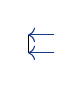
\begin{tikzpicture}[x=.35em,y=.65em,baseline=-.5ex]\draw (0,0)--(0,1);\draw[->,color=blue] (2.7,1)--(0,1);\draw[->,color=blue] (2.7,0)--(0,0);\end{tikzpicture}} \qquad \mathrm{Homadd}((a_i)_{i\hand{\in} I},(b_j)_{j\hand{\in} J}) = \hand{\{}(u_{ij})_{(i,j)\hand{\in} I\times J} \hand{\mid} u_{ij} \hand{\in} \]
% Hand-drawn continuation cue wraps the second formula row and points upward.
\[ 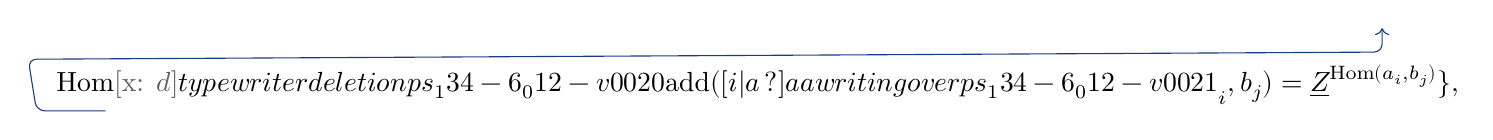
\begin{tikzpicture}[baseline=(continuation.base)]\node[inner sep=2pt] (continuation) {\ensuremath{\mathrm{Hom}\var{\xout{d}}{}{typewriter deletion}{ps_134-6_012-v0020}\mathrm{add}(\var{\over{\unsure{i|a}}{a}}{\hand{a}}{writing over}{ps_134-6_012-v0021}_i,b_j) = \underline{Z}^{\mathrm{Hom}(a_i,b_j)}\hand{\}} \hand{,}}};\draw[rounded corners=3pt,->,color=blue] ([xshift=2em]continuation.south west)--([xshift=-.5em]continuation.south west)--([xshift=-.8em]continuation.north west)--([xshift=-3em,yshift=.6ex]continuation.north east)--++(0,2ex);\end{tikzpicture} \]
while composition of maps is defined by the composition of matrices.
We thus get a new category Add(B) and a functor
\[ (4) \qquad B \hand{\longrightarrow} \mathrm{Add}(B) \ , \]

\margin{12}

% Visual collation: both supplied image halves inspected; see CHECK_DECISIONS_134_7_8.tsv.

%% END SOURCE ps_134-6_012
\ifnum\EditionMode=1
\psapparatusstart
\psentry{ps_134-6_012-v0001}{1}{typewriter deletion}{\xout{canonical}}{}{The typewriter strikes out this material; it leaves the corrected running text.}
\psentry{ps_134-6_012-v0002}{2}{typewriter deletion}{\xout{for any}}{}{The typewriter strikes out this material; it leaves the corrected running text.}
\psentry{ps_134-6_012-v0003}{3}{typewriter deletion}{\xout{category B}}{}{The typewriter strikes out this material; it leaves the corrected running text.}
\psentry{ps_134-6_012-v0004}{4}{typewriter overwriting}{\over[typed]{i}{b}}{b}{The superposed typed reading replaces the underlying reading.}
\psentry{ps_134-6_012-v0005}{5}{typewriter overwriting}{\over[typed]{b}{i}}{i}{The superposed typed reading replaces the underlying reading.}
\psentry{ps_134-6_012-v0006}{6}{writing over}{$\over{B}{B}$}{$\hand{B}$}{The superposed handwritten reading replaces the underlying reading.}
\psentry{ps_134-6_012-v0007}{7}{typewriter deletion}{\xout{fa}}{}{The typewriter strikes out this material; it leaves the corrected running text.}
\psentry{ps_134-6_012-v0008}{8}{insertion}{\inserted{of B}}{\hand{of B}}{The handwritten insertion is incorporated at its indicated position; insertion brackets leave the running text.}
\psentry{ps_134-6_012-v0009}{9}{typewriter overwriting}{$\over[typed]{a}{b}$}{$b$}{The superposed typed reading replaces the underlying reading.}
\psentry{ps_134-6_012-v0010}{10}{deletion}{\deleted{of B}}{}{The author cancels this material by hand; it leaves the corrected running text.}
\psentry{ps_134-6_012-v0011}{11}{typewriter overwriting}{$\over[typed]{1}{2}$}{$2$}{The superposed typed reading replaces the underlying reading.}
\psentry{ps_134-6_012-v0012}{12}{typewriter deletion}{\xout{when}}{}{The typewriter strikes out this material; it leaves the corrected running text.}
\psentry{ps_134-6_012-v0013}{13}{writing over}{\over{n}{n}}{\hand{n}}{The superposed handwritten reading replaces the underlying reading.}
\psentry{ps_134-6_012-v0014}{14}{writing over}{\over{s}{s}}{\hand{s}}{The superposed handwritten reading replaces the underlying reading.}
\psentry{ps_134-6_012-v0015}{15}{typewriter overwriting}{\over[typed]{h}{b}}{b}{The superposed typed reading replaces the underlying reading.}
\psentry{ps_134-6_012-v0016}{16}{typewriter overwriting}{\over[typed]{\unsure{u|v}}{y}}{y}{The superposed typed reading replaces the underlying reading.}
\psentry{ps_134-6_012-v0017}{17}{writing over}{\over{w}{w}}{\hand{w}}{The superposed handwritten reading replaces the underlying reading.}
\psentry{ps_134-6_012-v0018}{18}{writing over}{\over{a}{a}}{\hand{a}}{The superposed handwritten reading replaces the underlying reading.}
\psentry{ps_134-6_012-v0019}{19}{writing over}{\over{\unsure{y}}{y}}{\hand{y}}{The superposed handwritten reading replaces the underlying reading.}
\psentry{ps_134-6_012-v0020}{20}{typewriter deletion}{$\xout{d}$}{}{The typewriter strikes out this material; it leaves the corrected running text.}
\psentry{ps_134-6_012-v0021}{21}{writing over}{$\over{\unsure{i|a}}{a}$}{$\hand{a}$}{The superposed handwritten reading replaces the underlying reading.}
\psapparatusend
\fi
\pssource{ps_134-6_013}{134-6/13}{https://grothendieck.umontpellier.fr/web/viewer.html?file=../134-6.pdf\#page=14}
\psnumber{ps_134-6_013-v0001}{1}
\psnumber{ps_134-6_013-v0002}{2}
\psnumber{ps_134-6_013-v0003}{3}
\psnumber{ps_134-6_013-v0004}{4}
\psnumber{ps_134-6_013-v0005}{5}
\psnumber{ps_134-6_013-v0006}{6}
\psnumber{ps_134-6_013-v0007}{7}
\psnumber{ps_134-6_013-v0008}{8}
\psnumber{ps_134-6_013-v0009}{9}
\psnumber{ps_134-6_013-v0010}{10}
\psnumber{ps_134-6_013-v0011}{11}
\psnumber{ps_134-6_013-v0012}{12}
\psnumber{ps_134-6_013-v0013}{13}
\psnumber{ps_134-6_013-v0014}{14}
\psnumber{ps_134-6_013-v0015}{15}
%% BEGIN SOURCE ps_134-6_013
% Pursuing Stacks (cotes 134-2 to 134-8): archive cote 134-6, site page 13 (PDF page 14), typescript page 332.
% typescript. Draft compared: ps5.tex:1989-2057.
% AI-transcribed by Claude Opus 5.5 (claude-opus-5-5, adaptive thinking, effort high), Message Batches API, batch ps3 (msgbatch_01XdFmuVVBAcgc7EFxdtCqsj), 2026-11-12; reviewed against both supplied scan halves; see CHECK_DECISIONS.tsv.
\scanpage{134-6/13}
\mspage{332}

it is immediately checked that Add(B) is an additive category \var{\over[typed]{t}{a}}{a}{typewriter overwriting}{ps_134-6_013-v0001}hd that
the functor (4) has the 2-universal property for functors from B into
any additive category, stated in yesterday's notes (p.330).

\uline{R$\overset{\illegible{1}}{\underset{\illegible{1}}{e}}$mark}. The same construction essentially applies when considering the
universal problem of mapping B into any k-\uline{additive} category M \var{\deleted{\illegible{1}}}{}{deletion}{ps_134-6_013-v0002} (where
k is any \var{\inserted[typed]{commutative}}{commutative}{typed insertion}{ps_134-6_013-v0003} ring with unit), i.e. an additive category M endowed with a
ring homomorphism
\[ k \hand{\longrightarrow} \mathrm{End}(\mathrm{id}_M) , \]
replacing \var{\inserted[typed]{$\underline{Z}$ by k}}{$\underline{Z}$ by k}{typed insertion}{ps_134-6_013-v0004} in formulas (1) and (3) \var{\xout{$\underline{Z}$ by k}}{}{typewriter deletion}{ps_134-6_013-v0005}. The ``abelianization'' ques-%
tions \var{\over[typed]{d}{t}}{t}{typewriter overwriting}{ps_134-6_013-v0006}euched at in yesterday's notes still make a sense in terms of
``k-linearization'' - a notion much in the spirit of our introduction
of a general basic localizer $\underline{W}$ , as the very notion of k-linearization
will give rise to a corresponding basic localizer $\underline{W}_k$ ...

Let's come back to the case when $B=A^o$ , A being a small category,
and to our question about chain complexes
\[ L. \quad \text{in} \quad Ch.(Add(A^o)) \]
giving rise to a commutative diagram (20) (p.328), up to isomorphism.
\var{\over{a}{A}}{\hand{A}}{writing over}{ps_134-6_013-v0007} pair
\[ (L. , \hand{\lambda}) , \]
where L. is a chain complex as above, and \hand{$\lambda$} a compatibility isomor-%
phism for the square in (20), could be suggestively called an
\uline{abelianizator} for the small category A. The question of existence,
and uniqueness up to homotopy say, of an abelianizator for A seems
especially relevant when A is a test category say, and hence $A^\wedge$ mode-%
lizes homotopy types. In any case, in terms of an abelianizator we
get an additive functor
(5) \qquad $L\colon A^\wedge_{ab} \hand{\longrightarrow} Ch.(Ab)$ ,
and the question arises whether this is compatible with weak equivalen-%
ces and quasi-isomorphisms\hand{;} \var{\xout{-}}{}{typewriter deletion}{ps_134-6_013-v0008} maybe even,\var{\xout{t}}{}{typewriter deletion}{ps_134-6_013-v0009} if \var{\deleted{it}}{}{deletion}{ps_134-6_013-v0010}\var{\inserted{this}}{\hand{this}}{insertion}{ps_134-6_013-v0011} is not automatic, we
should insist it \var{\xout{he}}{}{typewriter deletion}{ps_134-6_013-v0012} holds when defining the notion of an abelianizator.
When this is OK, then by passing to localizations we deduce from (5)
a functor
(6) \qquad $\mathrm{H}\underset{\mathrm{o}}{\mathrm{o}}\mathrm{tab}_A \hand{\longrightarrow} \mathrm{Hotab}$ , \margin{\unsure{,}}
i.e. a functor (14) as looked for in yesterday's notes, giving rise
to \var{\xout{a}}{}{typewriter deletion}{ps_134-6_013-v0013}\var{\inserted[typed]{the}}{the}{typed insertion}{ps_134-6_013-v0014} commutative diagram (19) (p.328) - whereas commutativity of
diagrams of the type \var{\over{1}{(}}{\hand{(}}{writing over}{ps_134-6_013-v0015}15) (p. 326) looks less obvious.

\margin{13}

% Visual collation: both supplied image halves inspected; see CHECK_DECISIONS_134_7_8.tsv.

%% END SOURCE ps_134-6_013
\ifnum\EditionMode=1
\psapparatusstart
\psentry{ps_134-6_013-v0001}{1}{typewriter overwriting}{\over[typed]{t}{a}}{a}{The superposed typed reading replaces the underlying reading.}
\psentry{ps_134-6_013-v0002}{2}{deletion}{\deleted{\illegible{1}}}{}{The author cancels this material by hand; it leaves the corrected running text.}
\psentry{ps_134-6_013-v0003}{3}{typed insertion}{\inserted[typed]{commutative}}{commutative}{The typed insertion is incorporated at its indicated position; insertion brackets leave the running text.}
\psentry{ps_134-6_013-v0004}{4}{typed insertion}{\inserted[typed]{$\underline{Z}$ by k}}{$\underline{Z}$ by k}{The typed insertion is incorporated at its indicated position; insertion brackets leave the running text.}
\psentry{ps_134-6_013-v0005}{5}{typewriter deletion}{\xout{$\underline{Z}$ by k}}{}{The typewriter strikes out this material; it leaves the corrected running text.}
\psentry{ps_134-6_013-v0006}{6}{typewriter overwriting}{\over[typed]{d}{t}}{t}{The superposed typed reading replaces the underlying reading.}
\psentry{ps_134-6_013-v0007}{7}{writing over}{\over{a}{A}}{\hand{A}}{The superposed handwritten reading replaces the underlying reading.}
\psentry{ps_134-6_013-v0008}{8}{typewriter deletion}{\xout{-}}{}{The typewriter strikes out this material; it leaves the corrected running text.}
\psentry{ps_134-6_013-v0009}{9}{typewriter deletion}{\xout{t}}{}{The typewriter strikes out this material; it leaves the corrected running text.}
\psentry{ps_134-6_013-v0010}{10}{deletion}{\deleted{it}}{}{The author cancels this material by hand; it leaves the corrected running text.}
\psentry{ps_134-6_013-v0011}{11}{insertion}{\inserted{this}}{\hand{this}}{The handwritten insertion is incorporated at its indicated position; insertion brackets leave the running text.}
\psentry{ps_134-6_013-v0012}{12}{typewriter deletion}{\xout{he}}{}{The typewriter strikes out this material; it leaves the corrected running text.}
\psentry{ps_134-6_013-v0013}{13}{typewriter deletion}{\xout{a}}{}{The typewriter strikes out this material; it leaves the corrected running text.}
\psentry{ps_134-6_013-v0014}{14}{typed insertion}{\inserted[typed]{the}}{the}{The typed insertion is incorporated at its indicated position; insertion brackets leave the running text.}
\psentry{ps_134-6_013-v0015}{15}{writing over}{\over{1}{(}}{\hand{(}}{The superposed handwritten reading replaces the underlying reading.}
\psapparatusend
\fi
\pssource{ps_134-6_014}{134-6/14}{https://grothendieck.umontpellier.fr/web/viewer.html?file=../134-6.pdf\#page=15}
\psnumber{ps_134-6_014-v0001}{1}
\psnumber{ps_134-6_014-v0002}{2}
\psnumber{ps_134-6_014-v0003}{3}
\psnumber{ps_134-6_014-v0004}{4}
\psnumber{ps_134-6_014-v0005}{5}
\psnumber{ps_134-6_014-v0006}{6}
\psnumber{ps_134-6_014-v0007}{7}
\psnumber{ps_134-6_014-v0008}{8}
\psnumber{ps_134-6_014-v0009}{9}
\psnumber{ps_134-6_014-v0010}{10}
\psnumber{ps_134-6_014-v0011}{11}
\psnumber{ps_134-6_014-v0012}{12}
\psnumber{ps_134-6_014-v0013}{13}
\psnumber{ps_134-6_014-v0014}{14}
\psnumber{ps_134-6_014-v0015}{15}
%% BEGIN SOURCE ps_134-6_014
% Pursuing Stacks (cotes 134-2 to 134-8): archive cote 134-6, site page 14 (PDF page 15), typescript page 333.
% typescript. Draft compared: ps5.tex:2041-2123.
% AI-transcribed by Claude Opus 5.5 (claude-opus-5-5, adaptive thinking, effort high), Message Batches API, batch ps3 (msgbatch_01XdFmuVVBAcgc7EFxdtCqsj), 2026-11-12; reviewed against both supplied scan halves; see CHECK_DECISIONS.tsv.
\scanpage{134-6/14}
\mspage{333}

When A is a finite product of copies taken from among the three
standard test categories \hand{$\Delta$},\hand{$\square$} ,\hand{\tikz[baseline=-0.5ex,x=0.7ex,y=0.9ex]{\draw (0,0) ellipse (0.75 and 1);\draw (0.2,0.95) .. controls (-0.6,0.25) and (-0.6,-0.2) .. (0,-1);}} ,the standard chain complex structure
on multicomplexes does furnish us with a \uline{``canonical''} \uline{abelianizator}
for A, which we may denote by $L\overset{A}{.}$ (as we did yesterday for A =\hand{$\Delta$} ).
This ``standard'' abelianizator has some very remarkable extra features
which I would like to pin down, \var{\xout{and}}{}{typewriter deletion}{ps_134-6_014-v0001} which ha\var{\over[typed]{\unsure{s|e}}{d}}{d}{typewriter overwriting}{ps_134-6_014-v0002} caused our rather narrow
focus in the notes of two days ago (section 91).

a) T$\overset{\illegible{1}}{h}$ere is a ``dimension map''
\[ (7) \qquad \dim:\ \mathrm{Ob}\,A \hand{\longrightarrow} \underline{N} \quad . \]
It can be described (in the particular case above at any rate) in terms
of the intrinsic category structure of A, by associating to every a in
A the ordered set
\[ (8) \qquad i(a) \;=\; \text{set of subobjects of a in A} \hand{\underset{\unsure{,}}{\illegible{1}}} \]
(NB not to be confused with subobjects of a in A\^{}, namely sieves in
a). \var{\deleted{which}}{}{deletion}{ps_134-6_014-v0003}\var{\inserted{This}}{\hand{This}}{insertion}{ps_134-6_014-v0004} is an ordered set with \var{\inserted{a}}{\hand{a}}{insertion}{ps_134-6_014-v0005} largest object \var{\xout{a}}{}{typewriter deletion}{ps_134-6_014-v0006} (namely a itself),
and which turns out to be finite (in the particular case\var{\xout{s}}{}{typewriter deletion}{ps_134-6_014-v0007} considered),
hence of finite combinatorial dimension (equal to the dimension of the
geometrical realization $|i(a)|$ ), and we have
\[ (9) \qquad \dim\,(a) \;=\; \dim\ i(a) \quad . \]

b) The n.th component $L_n$ of $L\overset{A}{.} = L.$ is given by
\[ (\var{\over{\unsure{9}}{1}}{\hand{1}}{writing over}{ps_134-6_014-v0008}0) \qquad L_n \;=\; \hand{\displaystyle\bigoplus}_{\dim(a)=n} a \quad , \]
(where the direct sum of course is taken in Add($A^{o}$) as in (2) above\hand{,})
which makes a sense when we assume (as is the case in our example)
that the map (7) \var{\inserted[typed]{is ``finite'', i.e.\hand{,}}}{is ``finite'', i.e.\hand{,}}{typed insertion}{ps_134-6_014-v0009} \var{\deleted{\xout{is of finite}}}{}{deletion}{ps_134-6_014-v0010} has finite fibers. For instance, in
all \var{\xout{cases}}{}{typewriter deletion}{ps_134-6_014-v0011} our ``standard'' cases, there is just \uline{one} object of A which is
of dimension 0, \var{\xout{namely}}{}{typewriter deletion}{ps_134-6_014-v0012} and this is also the final object.

c) The differential operator
\[ \hand{(11)} \qquad d_n:\ L_n \hand{\longrightarrow} L_{n-1} \]
can be obtained in the following way. We have \var{\xout{t}}{}{typewriter deletion}{ps_134-6_014-v0013}only to describe $d_n$ on
each summand a of $L_n$ i.e. by (10) on each a \hand{in} \var{\deleted{\xout{$A\illegible{1}\quad a\quad\mathrm{Ob}A\quad\dim a$}}}{}{deletion}{ps_134-6_014-v0014}
\[ \var{\xout{\illegible{1}}}{}{typewriter deletion}{ps_134-6_014-v0015} \ (12) \qquad A_n = \hand{\{}\, a \hand{\in} \mathrm{Ob}\,A \hand{|} \dim a = n \hand{\}}. \]
In view of (3), this restriction $d_n$ \hand{$|$} a can be described as a linear
combination of elements in the disjoint sum of the sets
\[ \mathrm{Hom}(b,a) \quad , \quad \text{with}\ \ b \hand{\in} An\text{-}1 \quad \hand{(a \in A_n\ \text{fixed}).} \]

\margin{14}

% Visual collation: both supplied image halves inspected; see CHECK_DECISIONS_134_7_8.tsv.

%% END SOURCE ps_134-6_014
\ifnum\EditionMode=1
\psapparatusstart
\psentry{ps_134-6_014-v0001}{1}{typewriter deletion}{\xout{and}}{}{The typewriter strikes out this material; it leaves the corrected running text.}
\psentry{ps_134-6_014-v0002}{2}{typewriter overwriting}{\over[typed]{\unsure{s|e}}{d}}{d}{The superposed typed reading replaces the underlying reading.}
\psentry{ps_134-6_014-v0003}{3}{deletion}{\deleted{which}}{}{The author cancels this material by hand; it leaves the corrected running text.}
\psentry{ps_134-6_014-v0004}{4}{insertion}{\inserted{This}}{\hand{This}}{The handwritten insertion is incorporated at its indicated position; insertion brackets leave the running text.}
\psentry{ps_134-6_014-v0005}{5}{insertion}{\inserted{a}}{\hand{a}}{The handwritten insertion is incorporated at its indicated position; insertion brackets leave the running text.}
\psentry{ps_134-6_014-v0006}{6}{typewriter deletion}{\xout{a}}{}{The typewriter strikes out this material; it leaves the corrected running text.}
\psentry{ps_134-6_014-v0007}{7}{typewriter deletion}{\xout{s}}{}{The typewriter strikes out this material; it leaves the corrected running text.}
\psentry{ps_134-6_014-v0008}{8}{writing over}{$\over{\unsure{9}}{1}$}{$\hand{1}$}{The superposed handwritten reading replaces the underlying reading.}
\psentry{ps_134-6_014-v0009}{9}{typed insertion}{\inserted[typed]{is ``finite'', i.e.\hand{,}}}{is ``finite'', i.e.\hand{,}}{The typed insertion is incorporated at its indicated position; insertion brackets leave the running text.}
\psentry{ps_134-6_014-v0010}{10}{deletion}{\deleted{\xout{is of finite}}}{}{The author cancels this material by hand; it leaves the corrected running text.}
\psentry{ps_134-6_014-v0011}{11}{typewriter deletion}{\xout{cases}}{}{The typewriter strikes out this material; it leaves the corrected running text.}
\psentry{ps_134-6_014-v0012}{12}{typewriter deletion}{\xout{namely}}{}{The typewriter strikes out this material; it leaves the corrected running text.}
\psentry{ps_134-6_014-v0013}{13}{typewriter deletion}{\xout{t}}{}{The typewriter strikes out this material; it leaves the corrected running text.}
\psentry{ps_134-6_014-v0014}{14}{deletion}{\deleted{\xout{$A\illegible{1}\quad a\quad\mathrm{Ob}A\quad\dim a$}}}{}{The author cancels this material by hand; it leaves the corrected running text.}
\psentry{ps_134-6_014-v0015}{15}{typewriter deletion}{$\xout{\illegible{1}}$}{}{The typewriter strikes out this material; it leaves the corrected running text.}
\psapparatusend
\fi
\pssource{ps_134-6_015}{134-6/15}{https://grothendieck.umontpellier.fr/web/viewer.html?file=../134-6.pdf\#page=16}
\psnumber{ps_134-6_015-v0001}{1}
\psnumber{ps_134-6_015-v0002}{2}
\psnumber{ps_134-6_015-v0003}{3}
\psnumber{ps_134-6_015-v0004}{4}
\psnumber{ps_134-6_015-v0005}{5}
\psnumber{ps_134-6_015-v0006}{6}
\psnumber{ps_134-6_015-v0007}{7}
\psnumber{ps_134-6_015-v0008}{8}
\psnumber{ps_134-6_015-v0009}{9}
\psnumber{ps_134-6_015-v0010}{10}
\psnumber{ps_134-6_015-v0011}{11}
\psnumber{ps_134-6_015-v0012}{12}
\psnumber{ps_134-6_015-v0013}{13}
\psnumber{ps_134-6_015-v0014}{14}
\psnumber{ps_134-6_015-v0015}{15}
\psnumber{ps_134-6_015-v0016}{16}
\psnumber{ps_134-6_015-v0017}{17}
\psnumber{ps_134-6_015-v0018}{18}
%% BEGIN SOURCE ps_134-6_015
% Pursuing Stacks (cotes 134-2 to 134-8): archive cote 134-6, site page 15 (PDF page 16), typescript page 334.
% typescript. Draft compared: ps5.tex:2103-2184.
% AI-transcribed by Claude Opus 5.5 (claude-opus-5-5, adaptive thinking, effort high), Message Batches API, batch ps3 (msgbatch_01XdFmuVVBAcgc7EFxdtCqsj), 2026-11-12; reviewed against both supplied scan halves; see CHECK_DECISIONS.tsv.
\scanpage{134-6/15}
\mspage{334}

This being \var{\xout{so}}{}{typewriter deletion}{ps_134-6_015-v0001} clear,  the non-zero coefficients which occur in this
linear combination are all $\pm$ 1 ,  and moreover the maps which target a
\[ b \hand{\longrightarrow} a \qquad (b \quad A_{n-1}) \]
which o\var{\over[typed]{\unsure{r}}{c}}{c}{typewriter overwriting}{ps_134-6_015-v0002}cur with non-zero coefficient are exactly \uline{all monomorphisms}
from objects b in $A_{n-1}$ into a.  Thus,  the differential operators are
known,  when we know ,  for a\var{\over{ny}{ll}}{\hand{ll}}{writing over}{ps_134-6_015-v0003} monomorphism\var{\over{s}{s}}{\hand{s}}{writing over}{ps_134-6_015-v0004} in A
(13) \qquad $\hand{\partial}: b \hand{\to} a$ \quad , \quad with \quad dim a = dim b + 1
(the so-called ``\uline{boundary maps}''),  the corresponding coefficient\hand{s}
(14) \qquad $\hand{\varepsilon_{\partial} \in \{}\pm 1\hand{\}}$ .
Instinct tells us,  at this point,  that we may get into trouble,  when
trying to define (in a more or less general case)  boundary operations
in such a way,  because of the ambiguity in the definition of subobjects\hand{,}
namely, \var{\deleted{by the}}{}{deletion}{ps_134-6_015-v0005} \var{\inserted{because of possible}}{\hand{because of possible}}{insertion}{ps_134-6_015-v0006} \uline{existence of isomorphisms which may not be identities.}
But precisely,  in the standard cases we are \var{\xout{using}}{}{typewriter deletion}{ps_134-6_015-v0007} copying from,  \uline{\var{\over[typed]{t}{a}}{a}{typewriter overwriting}{ps_134-6_015-v0008}ny}
\uline{isomorphism is an identity}\hand{!}

d)  For describing the ``signatures'' (14),  in one of the ``standard''
cases,  we still need to remark that  for any a in A,  we have
(15) \qquad i(a)  is an n-cell\var{\xout{s}}{}{typewriter deletion}{ps_134-6_015-v0009},  with  n = dim (a) \quad ,
and the choice of the \var{\xout{signs}}{}{typewriter deletion}{ps_134-6_015-v0010} signatures will be determined by a choice
of orientations
(16) \qquad $\hand{\omega}_a$ an \uline{orientation} of the n-cell $\hand{|}i(a)\hand{|}$ \quad ,
(a notion which could be given a purely combinatorial definition,  \var{\over[typed]{h}{b}}{b}{typewriter overwriting}{ps_134-6_015-v0011}\var{\over[typed]{\unsure{u|v}}{y}}{y}{typewriter overwriting}{ps_134-6_015-v0012}
induction on the dimension of a given ord\var{\over[typed]{r}{e}}{e}{typewriter overwriting}{ps_134-6_015-v0013}\var{\over[typed]{e}{r}}{r}{typewriter overwriting}{ps_134-6_015-v0014}ed set whose geometrical
realization is a va\var{\over[typed]{t}{r}}{r}{typewriter overwriting}{ps_134-6_015-v0015}iety ...).  We the\hand{n} get the\unsure{\hand{n}|\var{\deleted{n}}{}{deletion}{ps_134-6_015-v0016}} ``\uline{Stokes rule}''
(17) \quad For a boundary map $\hand{\partial}: b \hand{\to} a$ \quad , $\hand{\varepsilon_{\partial}} = +1$  iff $\hand{\omega}_b$ is ``induced'' à
la Stokes by $\hand{\omega}_a$\hand{,} via the induced orientation on the boundary
of  i(a) \hand{(} which is the union of the images of all  i(b) 's ,
for all boundary operations with target a\hand{)}.

Whether or not we are in a ``standard'' case,  if A is any category,
such that for any object a of A,  the ordered set i(a)  of it's subob-%
jects in A  is finite,  and it's geometrical realization is an n-cell
( call n the ``dimension'' of a) ,  and if moreover for a given n,  the
set $A_n$ of objects with dimension n is finite,  and also (to be on the
safe side !)  \var{\deleted{we}}{}{deletion}{ps_134-6_015-v0017} assum\var{\over{e}{ing}}{\hand{ing}}{writing over}{ps_134-6_015-v0018} that all isomorphisms are identities,  then
for \uline{any} choice  of orientations (16),  giving rise to a system of

\margin{15}

% Visual collation: both supplied image halves inspected; see CHECK_DECISIONS_134_7_8.tsv.

%% END SOURCE ps_134-6_015
\ifnum\EditionMode=1
\psapparatusstart
\psentry{ps_134-6_015-v0001}{1}{typewriter deletion}{\xout{so}}{}{The typewriter strikes out this material; it leaves the corrected running text.}
\psentry{ps_134-6_015-v0002}{2}{typewriter overwriting}{\over[typed]{\unsure{r}}{c}}{c}{The superposed typed reading replaces the underlying reading.}
\psentry{ps_134-6_015-v0003}{3}{writing over}{\over{ny}{ll}}{\hand{ll}}{The superposed handwritten reading replaces the underlying reading.}
\psentry{ps_134-6_015-v0004}{4}{writing over}{\over{s}{s}}{\hand{s}}{The superposed handwritten reading replaces the underlying reading.}
\psentry{ps_134-6_015-v0005}{5}{deletion}{\deleted{by the}}{}{The author cancels this material by hand; it leaves the corrected running text.}
\psentry{ps_134-6_015-v0006}{6}{insertion}{\inserted{because of possible}}{\hand{because of possible}}{The handwritten insertion is incorporated at its indicated position; insertion brackets leave the running text.}
\psentry{ps_134-6_015-v0007}{7}{typewriter deletion}{\xout{using}}{}{The typewriter strikes out this material; it leaves the corrected running text.}
\psentry{ps_134-6_015-v0008}{8}{typewriter overwriting}{\over[typed]{t}{a}}{a}{The superposed typed reading replaces the underlying reading.}
\psentry{ps_134-6_015-v0009}{9}{typewriter deletion}{\xout{s}}{}{The typewriter strikes out this material; it leaves the corrected running text.}
\psentry{ps_134-6_015-v0010}{10}{typewriter deletion}{\xout{signs}}{}{The typewriter strikes out this material; it leaves the corrected running text.}
\psentry{ps_134-6_015-v0011}{11}{typewriter overwriting}{\over[typed]{h}{b}}{b}{The superposed typed reading replaces the underlying reading.}
\psentry{ps_134-6_015-v0012}{12}{typewriter overwriting}{\over[typed]{\unsure{u|v}}{y}}{y}{The superposed typed reading replaces the underlying reading.}
\psentry{ps_134-6_015-v0013}{13}{typewriter overwriting}{\over[typed]{r}{e}}{e}{The superposed typed reading replaces the underlying reading.}
\psentry{ps_134-6_015-v0014}{14}{typewriter overwriting}{\over[typed]{e}{r}}{r}{The superposed typed reading replaces the underlying reading.}
\psentry{ps_134-6_015-v0015}{15}{typewriter overwriting}{\over[typed]{t}{r}}{r}{The superposed typed reading replaces the underlying reading.}
\psentry{ps_134-6_015-v0016}{16}{deletion}{\deleted{n}}{}{The author cancels this material by hand; it leaves the corrected running text.}
\psentry{ps_134-6_015-v0017}{17}{deletion}{\deleted{we}}{}{The author cancels this material by hand; it leaves the corrected running text.}
\psentry{ps_134-6_015-v0018}{18}{writing over}{\over{e}{ing}}{\hand{ing}}{The superposed handwritten reading replaces the underlying reading.}
\psapparatusend
\fi
\pssource{ps_134-6_016}{134-6/16}{https://grothendieck.umontpellier.fr/web/viewer.html?file=../134-6.pdf\#page=17}
\psnumber{ps_134-6_016-v0001}{1}
\psnumber{ps_134-6_016-v0002}{2}
\psnumber{ps_134-6_016-v0003}{3}
\psnumber{ps_134-6_016-v0004}{4}
\psnumber{ps_134-6_016-v0005}{5}
\psnumber{ps_134-6_016-v0006}{6}
\psnumber{ps_134-6_016-v0007}{7}
\psnumber{ps_134-6_016-v0008}{8}
\psnumber{ps_134-6_016-v0009}{9}
\psnumber{ps_134-6_016-v0010}{10}
\psnumber{ps_134-6_016-v0011}{11}
\psnumber{ps_134-6_016-v0012}{12}
\psnumber{ps_134-6_016-v0013}{13}
\psnumber{ps_134-6_016-v0014}{14}
\psnumber{ps_134-6_016-v0015}{15}
\psnumber{ps_134-6_016-v0016}{16}
\psnumber{ps_134-6_016-v0017}{17}
\psnumber{ps_134-6_016-v0018}{18}
\psnumber{ps_134-6_016-v0019}{19}
\psnumber{ps_134-6_016-v0020}{20}
\psnumber{ps_134-6_016-v0021}{21}
\psnumber{ps_134-6_016-v0022}{22}
\psnumber{ps_134-6_016-v0023}{23}
\psnumber{ps_134-6_016-v0024}{24}
\psnumber{ps_134-6_016-v0025}{25}
\psnumber{ps_134-6_016-v0026}{26}
\psnumber{ps_134-6_016-v0027}{27}
\psnumber{ps_134-6_016-v0028}{28}
\psnumber{ps_134-6_016-v0029}{29}
\psnumber{ps_134-6_016-v0030}{30}
%% BEGIN SOURCE ps_134-6_016
% Pursuing Stacks (cotes 134-2 to 134-8): archive cote 134-6, site page 16 (PDF page 17), typescript page 335.
% typescript. Draft compared: ps5.tex:2169-2241.
% AI-transcribed by Claude Opus 5.5 (claude-opus-5-5, adaptive thinking, effort high), Message Batches API, batch ps3 (msgbatch_01XdFmuVVBAcgc7EFxdtCqsj), 2026-11-12; reviewed against both supplied scan halves; see CHECK_DECISIONS.tsv.
\scanpage{134-6/16}
\mspage{335}

signatures (13) by the ``Stokes rule'' (17), the corresponding operators
(11) do turn the family $(L_n)$ into a chain complex, na\var{\over[typed]{\unsure{e}}{m}}{m}{typewriter overwriting}{ps_134-6_016-v0001}\var{\over[typed]{\unsure{m}}{e}}{e}{typewriter overwriting}{ps_134-6_016-v0002}ly we have
the relations
\[ (18) \qquad d_{n-1}d_n = 0 \quad \hand{\unsure{,|.}} \]
\var{\over{\unsure{It}}{This}}{\hand{This}}{writing over}{ps_134-6_016-v0003} follows immediately from the well-\var{\over[typed]{\illegible{1}}{k}}{k}{typewriter overwriting}{ps_134-6_016-v0004}nown anticommutativity property
of \var{\xout{induction}}{}{typewriter deletion}{ps_134-6_016-v0005} (twofold) induction of orientation on boundaries.

Things are a little more delicate if we do'nt assume that isomor-%
phisms are identities, even if (by compens\unsure{q|a}tion) we \var{\inserted[typed]{should}}{should}{typed insertion}{ps_134-6_016-v0006} insist that two
distinct objects are never isomorphic. To define $d_{\hand{n}}$ , we then must
\uline{cho\var{\inserted[typed]{o}}{o}{typed insertion}{ps_134-6_016-v0007}se}, for any subobject \var{\over{b}{$\beta$}}{\hand{$\beta$}}{writing over}{ps_134-6_016-v0008} of dimension n-1 of \var{\xout{the}}{}{typewriter deletion}{ps_134-6_016-v0009} an object \var{\over{a}{$\unsure{a|\alpha}$}}{\hand{$\unsure{a|\alpha}$}}{writing over}{ps_134-6_016-v0010} of
dimension n, \var{\inserted[typed]{just \uline{one}}}{just \uline{one}}{typed insertion}{ps_134-6_016-v0011} \var{\xout{a}}{}{typewriter deletion}{ps_134-6_016-v0012} representative monomorphism (13) of \hand{$\beta$}. The coherence
condition then needed in order to get (18), is that \var{\xout{for}}{}{typewriter deletion}{ps_134-6_016-v0013} any \var{\xout{two such}}{}{typewriter deletion}{ps_134-6_016-v0014}
square diagram
% Hand-drawn arrows are marked blue; typed objects remain plain.
\[ (19) \qquad \diagram{\begin{tikzcd}[sep=small]
 \& \var{\over{\unsure{e|a}}{c}}{\hand{c}}{writing over}{ps_134-6_016-v0015} \ar[color=blue,dl] \ar[color=blue,dr] \& \\
 b \ar[color=blue,dr] \& \& b\hand{'} \ar[color=blue,dl] \\
 \& a \&
\end{tikzcd}} \]
made up with such restricted boundary maps, should commute -- a some-%
what delicate condition, presumably hard to insure, for the choices
involved for defining the ``strict'' boundary maps in A.

In one case as in the other, we are very close of course of the
set up envisioned in section 91 - it would'nt be hard even to \var{\xout{subordi\unsure{n}}}{}{typewriter deletion}{ps_134-6_016-v0016}
fit the case considered here into this set up, if we make the slight
extra assumption th\var{\over[typed]{e}{a}}{a}{typewriter overwriting}{ps_134-6_016-v0017}\var{\over[typed]{n}{t}}{t}{typewriter overwriting}{ps_134-6_016-v0018} any map in A factors into an ep\var{\xout{o}}{}{typewriter deletion}{ps_134-6_016-v0019}imorphism-with-%
section, followed by a monomorphism (which is true indeed in the
``standard'' cases), which will ensure that for varying a, i(a) is indeed
a functor with values in (Ord), as stated in loc. cit. But from the
point of view of construction of abelianizators, it would seem that
the e\var{\over[typed]{i}{x}}{x}{typewriter overwriting}{ps_134-6_016-v0020}\var{\over[typed]{x}{i}}{i}{typewriter overwriting}{ps_134-6_016-v0021}\var{\over[typed]{t}{s}}{s}{typewriter overwriting}{ps_134-6_016-v0022}\var{\over[typed]{s}{t}}{t}{typewriter overwriting}{ps_134-6_016-v0023}\var{\over[typed]{n}{e}}{e}{typewriter overwriting}{ps_134-6_016-v0024}\var{\over[typed]{e}{n}}{n}{typewriter overwriting}{ps_134-6_016-v0025}ce of \var{\over{a}{the}}{\hand{the}}{writing over}{ps_134-6_016-v0026} functor
\[ \hand{(20)} \qquad i: A \hand{\longrightarrow} (\mathrm{Ord}) \]
is irrelevant.

O\var{\over[typed]{r}{u}}{u}{typewriter overwriting}{ps_134-6_016-v0027}r main question now, of course, is about \uline{the chain complex L.}
\uline{being an abelianizator or not}. The question is interesting even in the
standard cases, by cho\var{\inserted{o}}{\hand{o}}{insertion}{ps_134-6_016-v0028}sing the orientations (16) in a way different
from the standard one. Are the corresponding chain\var{\xout{s}}{}{typewriter deletion}{ps_134-6_016-v0029} complexes in
Add($A^{\mathrm{o}}$) necessarily chain-homotopic ?

It just occurs to me that \var{\inserted{indeed,}}{\hand{indeed,}}{insertion}{ps_134-6_016-v0030} between the chain complexes

\margin{16}

% Visual collation: both supplied image halves inspected; see CHECK_DECISIONS_134_7_8.tsv.

%% END SOURCE ps_134-6_016
\ifnum\EditionMode=1
\psapparatusstart
\psentry{ps_134-6_016-v0001}{1}{typewriter overwriting}{\over[typed]{\unsure{e}}{m}}{m}{The superposed typed reading replaces the underlying reading.}
\psentry{ps_134-6_016-v0002}{2}{typewriter overwriting}{\over[typed]{\unsure{m}}{e}}{e}{The superposed typed reading replaces the underlying reading.}
\psentry{ps_134-6_016-v0003}{3}{writing over}{\over{\unsure{It}}{This}}{\hand{This}}{The superposed handwritten reading replaces the underlying reading.}
\psentry{ps_134-6_016-v0004}{4}{typewriter overwriting}{\over[typed]{\illegible{1}}{k}}{k}{The superposed typed reading replaces the underlying reading.}
\psentry{ps_134-6_016-v0005}{5}{typewriter deletion}{\xout{induction}}{}{The typewriter strikes out this material; it leaves the corrected running text.}
\psentry{ps_134-6_016-v0006}{6}{typed insertion}{\inserted[typed]{should}}{should}{The typed insertion is incorporated at its indicated position; insertion brackets leave the running text.}
\psentry{ps_134-6_016-v0007}{7}{typed insertion}{\inserted[typed]{o}}{o}{The typed insertion is incorporated at its indicated position; insertion brackets leave the running text.}
\psentry{ps_134-6_016-v0008}{8}{writing over}{\over{b}{$\beta$}}{\hand{$\beta$}}{The superposed handwritten reading replaces the underlying reading.}
\psentry{ps_134-6_016-v0009}{9}{typewriter deletion}{\xout{the}}{}{The typewriter strikes out this material; it leaves the corrected running text.}
\psentry{ps_134-6_016-v0010}{10}{writing over}{\over{a}{$\unsure{a|\alpha}$}}{\hand{$\unsure{a|\alpha}$}}{The superposed handwritten reading replaces the underlying reading.}
\psentry{ps_134-6_016-v0011}{11}{typed insertion}{\inserted[typed]{just \uline{one}}}{just \uline{one}}{The typed insertion is incorporated at its indicated position; insertion brackets leave the running text.}
\psentry{ps_134-6_016-v0012}{12}{typewriter deletion}{\xout{a}}{}{The typewriter strikes out this material; it leaves the corrected running text.}
\psentry{ps_134-6_016-v0013}{13}{typewriter deletion}{\xout{for}}{}{The typewriter strikes out this material; it leaves the corrected running text.}
\psentry{ps_134-6_016-v0014}{14}{typewriter deletion}{\xout{two such}}{}{The typewriter strikes out this material; it leaves the corrected running text.}
\psentry{ps_134-6_016-v0015}{15}{writing over}{$\over{\unsure{e|a}}{c}$}{$\hand{c}$}{The superposed handwritten reading replaces the underlying reading.}
\psentry{ps_134-6_016-v0016}{16}{typewriter deletion}{\xout{subordi\unsure{n}}}{}{The typewriter strikes out this material; it leaves the corrected running text.}
\psentry{ps_134-6_016-v0017}{17}{typewriter overwriting}{\over[typed]{e}{a}}{a}{The superposed typed reading replaces the underlying reading.}
\psentry{ps_134-6_016-v0018}{18}{typewriter overwriting}{\over[typed]{n}{t}}{t}{The superposed typed reading replaces the underlying reading.}
\psentry{ps_134-6_016-v0019}{19}{typewriter deletion}{\xout{o}}{}{The typewriter strikes out this material; it leaves the corrected running text.}
\psentry{ps_134-6_016-v0020}{20}{typewriter overwriting}{\over[typed]{i}{x}}{x}{The superposed typed reading replaces the underlying reading.}
\psentry{ps_134-6_016-v0021}{21}{typewriter overwriting}{\over[typed]{x}{i}}{i}{The superposed typed reading replaces the underlying reading.}
\psentry{ps_134-6_016-v0022}{22}{typewriter overwriting}{\over[typed]{t}{s}}{s}{The superposed typed reading replaces the underlying reading.}
\psentry{ps_134-6_016-v0023}{23}{typewriter overwriting}{\over[typed]{s}{t}}{t}{The superposed typed reading replaces the underlying reading.}
\psentry{ps_134-6_016-v0024}{24}{typewriter overwriting}{\over[typed]{n}{e}}{e}{The superposed typed reading replaces the underlying reading.}
\psentry{ps_134-6_016-v0025}{25}{typewriter overwriting}{\over[typed]{e}{n}}{n}{The superposed typed reading replaces the underlying reading.}
\psentry{ps_134-6_016-v0026}{26}{writing over}{\over{a}{the}}{\hand{the}}{The superposed handwritten reading replaces the underlying reading.}
\psentry{ps_134-6_016-v0027}{27}{typewriter overwriting}{\over[typed]{r}{u}}{u}{The superposed typed reading replaces the underlying reading.}
\psentry{ps_134-6_016-v0028}{28}{insertion}{\inserted{o}}{\hand{o}}{The handwritten insertion is incorporated at its indicated position; insertion brackets leave the running text.}
\psentry{ps_134-6_016-v0029}{29}{typewriter deletion}{\xout{s}}{}{The typewriter strikes out this material; it leaves the corrected running text.}
\psentry{ps_134-6_016-v0030}{30}{insertion}{\inserted{indeed,}}{\hand{indeed,}}{The handwritten insertion is incorporated at its indicated position; insertion brackets leave the running text.}
\psapparatusend
\fi
\pssource{ps_134-6_017}{134-6/17}{https://grothendieck.umontpellier.fr/web/viewer.html?file=../134-6.pdf\#page=18}
\psnumber{ps_134-6_017-v0001}{1}
\psnumber{ps_134-6_017-v0002}{2}
\psnumber{ps_134-6_017-v0003}{3}
\psnumber{ps_134-6_017-v0004}{4}
\psnumber{ps_134-6_017-v0005}{5}
\psnumber{ps_134-6_017-v0006}{6}
\psnumber{ps_134-6_017-v0007}{7}
\psnumber{ps_134-6_017-v0008}{8}
\psnumber{ps_134-6_017-v0009}{9}
\psnumber{ps_134-6_017-v0010}{10}
\psnumber{ps_134-6_017-v0011}{11}
\psnumber{ps_134-6_017-v0012}{12}
\psnumber{ps_134-6_017-v0013}{13}
\psnumber{ps_134-6_017-v0014}{14}
\psnumber{ps_134-6_017-v0015}{15}
\psnumber{ps_134-6_017-v0016}{16}
\psnumber{ps_134-6_017-v0017}{17}
\psnumber{ps_134-6_017-v0018}{18}
\psnumber{ps_134-6_017-v0019}{19}
\psnumber{ps_134-6_017-v0020}{20}
%% BEGIN SOURCE ps_134-6_017
% Pursuing Stacks (cotes 134-2 to 134-8): archive cote 134-6, site page 17 (PDF page 18), typescript page 336.
% typescript. Draft compared: ps5.tex:2221-2291.
% AI-transcribed by Claude Opus 5.5 (claude-opus-5-5, adaptive thinking, effort high), Message Batches API, batch ps3 (msgbatch_01XdFmuVVBAcgc7EFxdtCqsj), 2026-11-12; reviewed against both supplied scan halves; see CHECK_DECISIONS.tsv.
\scanpage{134-6/17}
\mspage{336}

(22) \[ L.^{\hand{\omega}}\var{\deleted{\hand{(\omega)}}}{}{deletion}{ps_134-6_017-v0001} = ((L_n)_{n\hand{\in}\underline{N}} \ , (d_n^{\hand{\omega}})_{n\hand{\in}\underline{N}} ) \]
associated to \var{\xout{the}}{}{typewriter deletion}{ps_134-6_017-v0002} all possible systems of orientations
(23) \[ \hand{\omega} = (\hand{\omega}_a)_{a\, \hand{\in}\, \var{\over[typed]{A}{O}}{O}{typewriter overwriting}{ps_134-6_017-v0003}b(A)} \]
of the various cells  i(a)  ,  there is a canonical \uline{transitive system}
of isomorphisms,  by defining the isomorphism
(24) \[ u_{\hand{\omega,\omega'}} : L. \hand{\xrightarrow{\sim}} L.\hand{'} \]
for two different choices \hand{$\omega, \omega'$} of systems of orientations,  by
\margin{\tikz[baseline=(m.base)]{\node[inner sep=2pt] (m) {$\varepsilon_a^{\omega,\omega'}$};\draw (m.center) ellipse (1.8em and 1.1em);}}
(25) \[ u_{\hand{\omega,\omega'}} \hand{\mid} a = \hand{\varepsilon}_a^{\hand{\omega,\omega'}} \mathrm{id}_a \ , \qquad \hand{\varepsilon}_a^{\hand{\omega,\omega'}} \hand{\in\{} \pm 1\hand{\}}\hand{,} \]
where  \uline{the sign}  \hand{$\varepsilon$}$_a^{\hand{\omega,\omega'}}$ is  \uline{equal to}\hand{+}1 \uline{or} -1,  \uline{according to whether}  \hand{$\omega$}$_a$  \uline{and}
\hand{$\omega$}$'_a$  \uline{are equal or not}.  It is immediate that  (24)  then is an isomor-%
phism\var{\deleted{\unsure{e|s}}}{}{deletion}{ps_134-6_017-v0004} componentwise,  respecting degrees,  and commu\var{\xout{ta}}{}{typewriter deletion}{ps_134-6_017-v0005}ting to the res-%
pective differ\var{\over[typed]{n}{e}}{e}{typewriter overwriting}{ps_134-6_017-v0006}\var{\over[typed]{e}{n}}{n}{typewriter overwriting}{ps_134-6_017-v0007}t\var{\over[typed]{a}{i}}{i}{typewriter overwriting}{ps_134-6_017-v0008}\var{\over[typed]{i}{a}}{a}{typewriter overwriting}{ps_134-6_017-v0009}l  operators.  Transitivity of the isomorphisms
(24) for a triple  (\hand{$\omega$} ,\hand{$\omega'$},\hand{$\omega''$})  is equally immediate.  This implies that
by this trans\var{\over[typed]{t}{i}}{i}{typewriter overwriting}{ps_134-6_017-v0010}\var{\over[typed]{i}{t}}{t}{typewriter overwriting}{ps_134-6_017-v0011}ive system of isomorphisms,  \uline{we may identify all the chai\hand{n}}
\uline{comple\var{\over[typed]{d}{x}}{x}{typewriter overwriting}{ps_134-6_017-v0012}es}  $L.^{\hand{\omega}}$  in Add(A$^{o}$) to a single chain complex,  canonically \var{\deleted{\xout{equiv}}}{}{deletion}{ps_134-6_017-v0013}
isomorphic to each $L.^{\hand{\omega}}$ ,  and which we may just designate by L. .  This
chain complex now is defined intrinsically in terms of the category
structure of A (up to canonical isomorphism),  in the ``safe'' case at
any rate when every isomorphism in A is an identity,  so that in the
constr\var{\over[typed]{a}{u}}{u}{typewriter overwriting}{ps_134-6_017-v0014}ction of $L.^{\hand{\omega}}$ there enters no other choice besides \hand{$\omega$}.  Otherwise\unsure{,}
as seen above (precedent page),  we must still suitably choose \var{\over[typed]{s}{t}}{t}{typewriter overwriting}{ps_134-6_017-v0015}\var{\over[typed]{e}{h}}{h}{typewriter overwriting}{ps_134-6_017-v0016}e so-%
called ``strict'' boundary operators  (13) ,  a\var{\over{h}{m}}{\hand{m}}{writing over}{ps_134-6_017-v0017}ong all monomorphisms
b \hand{$\hookrightarrow$} a  in A such that  dim a = dim b + 1 .

In the first case say (isomorphisms being identities),  all con-%
ditions considered for A are stable under finite products,  that's why
in terms of the three standard cases of \hand{$\Delta$}, \hand{$\square$} and \hand{\tikz[baseline=-0.5ex,x=0.7ex,y=0.9ex]{\draw (0,0) ellipse (0.75 and 1);\draw (0.2,0.95) .. controls (-0.6,0.25) and (-0.6,-0.2) .. (0,-1);}},  we could con-%
struct others by taking finite products.  The three standard test catego-%
ries \var{\xout{\unsure{ar}e}}{}{typewriter deletion}{ps_134-6_017-v0018} may be viewed as particularly ``economic'' or skillful ways of
``cutting out'' a suitable bunch of cellular decompositions\hand{,} and \var{\inserted{of}}{\hand{of}}{insertion}{ps_134-6_017-v0019} elimina-%
ting automorphisms (by total ordering of vertices and the like ...),
so as to insure\hand{:} a) that isomorphisms in A are identities ,  b)  the
canonical chain complex L.  in Add(A$^{o}$)  is an abelianizator,  and  c)
A moreover is a strict test category,  and even a contractor.  On the
other hand,  as all these conditions  (plus the condition (15) of course
about the i(a)' s  representing n-cells)  \var{\deleted{all these \xout{conditions are stabl\illegible{1}}}}{}{deletion}{ps_134-6_017-v0020}

\margin{17}

% Visual collation: both supplied image halves inspected; see CHECK_DECISIONS_134_7_8.tsv.

%% END SOURCE ps_134-6_017
\ifnum\EditionMode=1
\psapparatusstart
\psentry{ps_134-6_017-v0001}{1}{deletion}{$\deleted{\hand{(\omega)}}$}{}{The author cancels this material by hand; it leaves the corrected running text.}
\psentry{ps_134-6_017-v0002}{2}{typewriter deletion}{\xout{the}}{}{The typewriter strikes out this material; it leaves the corrected running text.}
\psentry{ps_134-6_017-v0003}{3}{typewriter overwriting}{$\over[typed]{A}{O}$}{$O$}{The superposed typed reading replaces the underlying reading.}
\psentry{ps_134-6_017-v0004}{4}{deletion}{\deleted{\unsure{e|s}}}{}{The author cancels this material by hand; it leaves the corrected running text.}
\psentry{ps_134-6_017-v0005}{5}{typewriter deletion}{\xout{ta}}{}{The typewriter strikes out this material; it leaves the corrected running text.}
\psentry{ps_134-6_017-v0006}{6}{typewriter overwriting}{\over[typed]{n}{e}}{e}{The superposed typed reading replaces the underlying reading.}
\psentry{ps_134-6_017-v0007}{7}{typewriter overwriting}{\over[typed]{e}{n}}{n}{The superposed typed reading replaces the underlying reading.}
\psentry{ps_134-6_017-v0008}{8}{typewriter overwriting}{\over[typed]{a}{i}}{i}{The superposed typed reading replaces the underlying reading.}
\psentry{ps_134-6_017-v0009}{9}{typewriter overwriting}{\over[typed]{i}{a}}{a}{The superposed typed reading replaces the underlying reading.}
\psentry{ps_134-6_017-v0010}{10}{typewriter overwriting}{\over[typed]{t}{i}}{i}{The superposed typed reading replaces the underlying reading.}
\psentry{ps_134-6_017-v0011}{11}{typewriter overwriting}{\over[typed]{i}{t}}{t}{The superposed typed reading replaces the underlying reading.}
\psentry{ps_134-6_017-v0012}{12}{typewriter overwriting}{\over[typed]{d}{x}}{x}{The superposed typed reading replaces the underlying reading.}
\psentry{ps_134-6_017-v0013}{13}{deletion}{\deleted{\xout{equiv}}}{}{The author cancels this material by hand; it leaves the corrected running text.}
\psentry{ps_134-6_017-v0014}{14}{typewriter overwriting}{\over[typed]{a}{u}}{u}{The superposed typed reading replaces the underlying reading.}
\psentry{ps_134-6_017-v0015}{15}{typewriter overwriting}{\over[typed]{s}{t}}{t}{The superposed typed reading replaces the underlying reading.}
\psentry{ps_134-6_017-v0016}{16}{typewriter overwriting}{\over[typed]{e}{h}}{h}{The superposed typed reading replaces the underlying reading.}
\psentry{ps_134-6_017-v0017}{17}{writing over}{\over{h}{m}}{\hand{m}}{The superposed handwritten reading replaces the underlying reading.}
\psentry{ps_134-6_017-v0018}{18}{typewriter deletion}{\xout{\unsure{ar}e}}{}{The typewriter strikes out this material; it leaves the corrected running text.}
\psentry{ps_134-6_017-v0019}{19}{insertion}{\inserted{of}}{\hand{of}}{The handwritten insertion is incorporated at its indicated position; insertion brackets leave the running text.}
\psentry{ps_134-6_017-v0020}{20}{deletion}{\deleted{all these \xout{conditions are stabl\illegible{1}}}}{}{The author cancels this material by hand; it leaves the corrected running text.}
\psapparatusend
\fi
\pssource{ps_134-6_018}{134-6/18}{https://grothendieck.umontpellier.fr/web/viewer.html?file=../134-6.pdf\#page=19}
\psnumber{ps_134-6_018-v0001}{1}
\psnumber{ps_134-6_018-v0002}{2}
\psnumber{ps_134-6_018-v0003}{3}
\psnumber{ps_134-6_018-v0004}{4}
\psnumber{ps_134-6_018-v0005}{5}
\psnumber{ps_134-6_018-v0006}{6}
\psnumber{ps_134-6_018-v0007}{7}
\psnumber{ps_134-6_018-v0008}{8}
\psnumber{ps_134-6_018-v0009}{9}
\psnumber{ps_134-6_018-v0010}{10}
\psnumber{ps_134-6_018-v0011}{11}
\psnumber{ps_134-6_018-v0012}{12}
\psnumber{ps_134-6_018-v0013}{13}
\psnumber{ps_134-6_018-v0014}{14}
\psnumber{ps_134-6_018-v0015}{15}
\psnumber{ps_134-6_018-v0016}{16}
\psnumber{ps_134-6_018-v0017}{17}
\psnumber{ps_134-6_018-v0018}{18}
%% BEGIN SOURCE ps_134-6_018
% Pursuing Stacks (cotes 134-2 to 134-8): archive cote 134-6, site page 18 (PDF page 19), typescript page 337.
% typescript. Draft compared: ps5.tex:2279-2334.
% AI-transcribed by Claude Opus 5.5 (claude-opus-5-5, adaptive thinking, effort high), Message Batches API, batch pilot (msgbatch_0189Nhf1xB615YWnztubtLfc), 2026-11-12; reviewed against both supplied scan halves; see CHECK_DECISIONS.tsv.
\scanpage{134-6/18}
\mspage{337}

\var{\deleted{properties}}{}{deletion}{ps_134-6_018-v0001} are stable under taking \var{\xout{pro binary}}{}{typewriter deletion}{ps_134-6_018-v0002} products (of finite non-%
empty families of categories $A_i$), hence in terms of the three standard
\var{\over[typed]{t}{c}}{c}{typewriter overwriting}{ps_134-6_018-v0003}ases, the possibility of satisfying them too by the ``multistandard''
test categories. I wonder if there are any other ways (up to equiva-%
lence). If we take categories such as $\hand{\widetilde{\Delta}}$ (non ordered simplices) we
still get contractors, but objects have non trivial automo\var{\xout{t}}{}{typewriter deletion}{ps_134-6_018-v0004}rphisms, and
if we take categories such as $\hand{\Delta}^{f}$ (ordered simplices without degenera-%
cy operations, only boundary maps) it is true that isomorphisms are
identities, but the category is no longer a test category \var{\xout{not even}}{}{typewriter deletion}{ps_134-6_018-v0005}\var{\inserted[typed]{but only}}{but only}{typed insertion}{ps_134-6_018-v0006} a
weak one.

If we do not insist on the rigidity assumption (isomorphisms are
identities), but on suitable choice of so called ``\uline{strict} boundary
operations'' within A , then it would seem after all that we do have
a lot more elbow freedom then it seemed, by the end of our reflections
on that matter two days ago (cf. p. 318), where the picture of the re-%
levant data and corresponding \var{\xout{structur}}{}{typewriter deletion}{ps_134-6_018-v0007} construction of chain complexes
was still a little confused. Let now A be the category called $A_o$ ih
loc. cit. We don't have to modify it in order to introduce orientati-%
ons of cells i(a) as extra structure and take account of this in defi-%
ning \var{\xout{new}}{}{typewriter deletion}{ps_134-6_018-v0008} a new notion of map\hand{s.} Therefore it is clear that A \uline{just as it}
\uline{i\var{\over[typed]{t}{s}}{s}{typewriter overwriting}{ps_134-6_018-v0009}, is a strict test category} (\var{\xout{but}}{}{typewriter deletion}{ps_134-6_018-v0010} presumably \uline{not} a contractor though).
T$\overset{\illegible{1}}{h}$ere is the problem of course of isomorphisms which are not identi-%
ties, and particularly of non trivial automorphisms - for instance
the object I (playing the part of the unit segment) has a non trivial
automorphism, the elimination of which does not look so trivial !
However, there \uline{is} a rather evident way of cutting out \uline{strict} bounda-%
ry maps, in a way as to satisfy the transitivity condition of p.335
- namely by taking boundary maps (13) $\hand{\partial}: b \hand{\to} a$ which a\var{\over[typed]{r}{r}}{r}{typewriter overwriting}{ps_134-6_018-v0011}e \uline{inclusions}
in the strict sense, namely the inclusion map of a\var{\xout{n}}{}{typewriter deletion}{ps_134-6_018-v0012} \uline{subset} of a , en-%
dowed with the induced order relation.

Thus there are many other \var{\xout{ways}}{}{typewriter deletion}{ps_134-6_018-v0013}\var{\inserted[typed]{cases}}{cases}{typed insertion}{ps_134-6_018-v0014} still than just multi-standard
test categories for getting a canonical chain complex $L.$ in Add($A^o$),
\var{\deleted{so that}}{}{deletion}{ps_134-6_018-v0015} \var{\inserted{and for whom now}}{\hand{and for whom now}}{insertion}{ps_134-6_018-v0016} the question makes sense as to whether $L.$ is an abelianiz\var{\over{\unsure{o|e}r}{ator}}{\hand{ator}}{writing over}{ps_134-6_018-v0017}.
In the construction above, we were careful to assume that the full
subcategory \var{\xout{a}}{}{typewriter deletion}{ps_134-6_018-v0018} A of (Ord), besides containing I , was stable under
finite products, so as to make sure it comes out as a test category.
T$\overset{\illegible{1}}{\underset{\illegible{1}}{h}}$e silly thing is that this condition is not satisfied by any one among
the standard test categories - thus it seems reasonable to try and

\margin{18}

% Visual collation: both supplied image halves inspected; see CHECK_DECISIONS_134_7_8.tsv.

%% END SOURCE ps_134-6_018
\ifnum\EditionMode=1
\psapparatusstart
\psentry{ps_134-6_018-v0001}{1}{deletion}{\deleted{properties}}{}{The author cancels this material by hand; it leaves the corrected running text.}
\psentry{ps_134-6_018-v0002}{2}{typewriter deletion}{\xout{pro binary}}{}{The typewriter strikes out this material; it leaves the corrected running text.}
\psentry{ps_134-6_018-v0003}{3}{typewriter overwriting}{\over[typed]{t}{c}}{c}{The superposed typed reading replaces the underlying reading.}
\psentry{ps_134-6_018-v0004}{4}{typewriter deletion}{\xout{t}}{}{The typewriter strikes out this material; it leaves the corrected running text.}
\psentry{ps_134-6_018-v0005}{5}{typewriter deletion}{\xout{not even}}{}{The typewriter strikes out this material; it leaves the corrected running text.}
\psentry{ps_134-6_018-v0006}{6}{typed insertion}{\inserted[typed]{but only}}{but only}{The typed insertion is incorporated at its indicated position; insertion brackets leave the running text.}
\psentry{ps_134-6_018-v0007}{7}{typewriter deletion}{\xout{structur}}{}{The typewriter strikes out this material; it leaves the corrected running text.}
\psentry{ps_134-6_018-v0008}{8}{typewriter deletion}{\xout{new}}{}{The typewriter strikes out this material; it leaves the corrected running text.}
\psentry{ps_134-6_018-v0009}{9}{typewriter overwriting}{\over[typed]{t}{s}}{s}{The superposed typed reading replaces the underlying reading.}
\psentry{ps_134-6_018-v0010}{10}{typewriter deletion}{\xout{but}}{}{The typewriter strikes out this material; it leaves the corrected running text.}
\psentry{ps_134-6_018-v0011}{11}{typewriter overwriting}{\over[typed]{r}{r}}{r}{The superposed typed reading replaces the underlying reading.}
\psentry{ps_134-6_018-v0012}{12}{typewriter deletion}{\xout{n}}{}{The typewriter strikes out this material; it leaves the corrected running text.}
\psentry{ps_134-6_018-v0013}{13}{typewriter deletion}{\xout{ways}}{}{The typewriter strikes out this material; it leaves the corrected running text.}
\psentry{ps_134-6_018-v0014}{14}{typed insertion}{\inserted[typed]{cases}}{cases}{The typed insertion is incorporated at its indicated position; insertion brackets leave the running text.}
\psentry{ps_134-6_018-v0015}{15}{deletion}{\deleted{so that}}{}{The author cancels this material by hand; it leaves the corrected running text.}
\psentry{ps_134-6_018-v0016}{16}{insertion}{\inserted{and for whom now}}{\hand{and for whom now}}{The handwritten insertion is incorporated at its indicated position; insertion brackets leave the running text.}
\psentry{ps_134-6_018-v0017}{17}{writing over}{\over{\unsure{o|e}r}{ator}}{\hand{ator}}{The superposed handwritten reading replaces the underlying reading.}
\psentry{ps_134-6_018-v0018}{18}{typewriter deletion}{\xout{a}}{}{The typewriter strikes out this material; it leaves the corrected running text.}
\psapparatusend
\fi
\pssource{ps_134-6_019}{134-6/19}{https://grothendieck.umontpellier.fr/web/viewer.html?file=../134-6.pdf\#page=20}
\psnumber{ps_134-6_019-v0001}{1}
\psnumber{ps_134-6_019-v0002}{2}
\psnumber{ps_134-6_019-v0003}{3}
\psnumber{ps_134-6_019-v0004}{4}
\psnumber{ps_134-6_019-v0005}{5}
\psnumber{ps_134-6_019-v0006}{6}
\psnumber{ps_134-6_019-v0007}{7}
\psnumber{ps_134-6_019-v0008}{8}
\psnumber{ps_134-6_019-v0009}{9}
\psnumber{ps_134-6_019-v0010}{10}
\psnumber{ps_134-6_019-v0011}{11}
\psnumber{ps_134-6_019-v0012}{12}
\psnumber{ps_134-6_019-v0013}{13}
\psnumber{ps_134-6_019-v0014}{14}
\psnumber{ps_134-6_019-v0015}{15}
\psnumber{ps_134-6_019-v0016}{16}
\psnumber{ps_134-6_019-v0017}{17}
\psnumber{ps_134-6_019-v0018}{18}
\psnumber{ps_134-6_019-v0019}{19}
\psnumber{ps_134-6_019-v0020}{20}
\psnumber{ps_134-6_019-v0021}{21}
\psnumber{ps_134-6_019-v0022}{22}
\psnumber{ps_134-6_019-v0023}{23}
%% BEGIN SOURCE ps_134-6_019
% Pursuing Stacks (cotes 134-2 to 134-8): archive cote 134-6, site page 19 (PDF page 20), typescript page 338.
% typescript. Draft compared: ps5.tex:2322-2388.
% AI-transcribed by Claude Opus 5.5 (claude-opus-5-5, adaptive thinking, effort high), Message Batches API, batch ps3 (msgbatch_01XdFmuVVBAcgc7EFxdtCqsj), 2026-11-12; reviewed against both supplied scan halves; see CHECK_DECISIONS.tsv.
\scanpage{134-6/19}
\mspage{338}
replace it by a suitable substitute,  such as the existence,  for any
two objects a and b in A,  of a cellular subdivision of $\hand{|}i(a)\hand{|}\times\hand{|}i(b)\hand{|}$ ,
made up with cells of the type $\hand{|}i(c)\hand{|}$,  and inducing on the latter the
given cellular structure of $\hand{|}i(c)\hand{|}$ .  The problem is now (besides get-%
ting or not an abelianizator $L.$ )  \uline{whether A is at any rate a weak test
category}  (in view of the example of $\hand{\Delta}^{f}$ ,  we can't expect \var{\inserted[typed]{now}}{now}{typed insertion}{ps_134-6_019-v0001} of course
\var{\xout{now}}{}{typewriter deletion}{ps_134-6_019-v0002} to get an actual test category).  Maybe I'll come back to this la-%
ter,  when writing down a proof for $\hand{\Delta}^{f}$  being a weak test category,  if
a more general result along these lines should come out alongside.

\uline{Remark\var{\over{s}{s}}{\hand{s}}{writing over}{ps_134-6_019-v0003}}.  \var{\deleted{1)}}{}{deletion}{ps_134-6_019-v0004}  I feel the canonical chain complex $L.$  in  $\mathrm{Add}(A^{o})$  con-%
structed in this section,  under suitable assumptions on the s\var{\over[typed]{e}{m}}{m}{typewriter overwriting}{ps_134-6_019-v0005}all cate-%
gory A,  merits a name of it's own.  We may call it the \uline{standard
abelianizator}  of A  -  but this is reasonable only if it turns out that
in al\var{\over{d}{l}}{\hand{l}}{writing over}{ps_134-6_019-v0006} cases when it can be constructed,  it is an abelianizator indeed.
Another convenient name may be the \uline{Dold-Puppe} \uline{\var{\over[typed]{O}{C}}{C}{typewriter overwriting}{ps_134-6_019-v0007}hain complex} ,  as \var{\xout{the}}{}{typewriter deletion}{ps_134-6_019-v0008}
in the three standard cases\hand{,} the standard Dold-Puppe construction of the
``normalization''  of an abelian complex \var{\inserted[typed]{(ss say)}}{(ss say)}{typed insertion}{ps_134-6_019-v0009} can be viewed as being performed
$\overset{\illegible{1}}{\text{\var{\over[typed]{o}{i}}{i}{typewriter overwriting}{ps_134-6_019-v0010}}}$n the ``universal'' case,  namely \var{\xout{\unsure{I|i|l}\illegible{1}}}{}{typewriter deletion}{ps_134-6_019-v0011}  $A^{o} \hand{\longrightarrow} \mathrm{Add}(A^{o})$,  and the correspon-%
ding ``full'' chain complex,  namely  $L.$  -  with this \var{\xout{slight}}{}{typewriter deletion}{ps_134-6_019-v0012} grain of
salt though that we have still to enlarge  $\mathrm{Add}(A^{o})$ slightly,  so as to
make it stable under taking direct summands corresponding to projectors.
But then it occurs to me that the name of Dold-Puppe chain complex is
much more suitable for the \uline{result of nor\var{\over[typed]{a}{m}}{m}{typewriter overwriting}{ps_134-6_019-v0013}\var{\over[typed]{m}{a}}{a}{typewriter overwriting}{ps_134-6_019-v0014}lization}  applied to $L.$  ,
\margin{\begin{tikzpicture}[x=.25em,y=1em,baseline={(0,3)}]\draw[->,rounded corners=2pt] (8,0)--(0,0)--(0,3);\end{tikzpicture}}which (if I got it right)  is the ``new'' complex discovered by Dold-Pup-%
pe,  together with the inverse construction,  whereas $L.$  had already \var{\inserted{been}}{\hand{been}}{insertion}{ps_134-6_019-v0015} \var{\deleted{be}}{}{deletion}{ps_134-6_019-v0016}
known for ages (even if not under it's u\var{\over[typed]{j}{n}}{n}{typewriter overwriting}{ps_134-6_019-v0017}iversal disguise ...).

\margin{\begin{tikzpicture}[x=.25em,y=1em,baseline={(0,3)}]\draw[->,rounded corners=2pt] (8,3)--(0,3)--(0,0);\end{tikzpicture}}\hand{94.} \var{\deleted{\hand{\unsure{2}.}}}{}{deletion}{ps_134-6_019-v0018}  In \var{\deleted{this}}{}{deletion}{ps_134-6_019-v0019}\var{\inserted{the last}}{\hand{the last}}{insertion}{ps_134-6_019-v0020} section,  as in the two preceding days,  our emphasis
\var{\xout{has been on}}{}{typewriter deletion}{ps_134-6_019-v0021} with abelianization of homotopy types has been to look at it
in terms of more or less arbitrary test categories and the corresponding
elementary modelizers,  are even in terms of arbitrary small categories.
This has caused as spinning a kind of dream for a while\hand{,} \var{\over{\unsure{t|w}ith}{with}}{\hand{with}}{writing over}{ps_134-6_019-v0022} the White-%
head and Dold Puppe theorems  and generalized bou\var{\inserted{n}}{\hand{n}}{insertion}{ps_134-6_019-v0023}dary maps as our main
thread.   Now this reminds me of a rather different line of thoughts
tied up with abelianization,  quite independently of playing around
with variable modelizers  -  a question which has been intriguing me
for a very long time now,  ever since  I  got acquainted a little with
the very notion of homotopy types,  and the corresponding homology and

\margin{19}

% Visual collation: both supplied image halves inspected; see CHECK_DECISIONS_134_7_8.tsv.

%% END SOURCE ps_134-6_019
\ifnum\EditionMode=1
\psapparatusstart
\psentry{ps_134-6_019-v0001}{1}{typed insertion}{\inserted[typed]{now}}{now}{The typed insertion is incorporated at its indicated position; insertion brackets leave the running text.}
\psentry{ps_134-6_019-v0002}{2}{typewriter deletion}{\xout{now}}{}{The typewriter strikes out this material; it leaves the corrected running text.}
\psentry{ps_134-6_019-v0003}{3}{writing over}{\over{s}{s}}{\hand{s}}{The superposed handwritten reading replaces the underlying reading.}
\psentry{ps_134-6_019-v0004}{4}{deletion}{\deleted{1)}}{}{The author cancels this material by hand; it leaves the corrected running text.}
\psentry{ps_134-6_019-v0005}{5}{typewriter overwriting}{\over[typed]{e}{m}}{m}{The superposed typed reading replaces the underlying reading.}
\psentry{ps_134-6_019-v0006}{6}{writing over}{\over{d}{l}}{\hand{l}}{The superposed handwritten reading replaces the underlying reading.}
\psentry{ps_134-6_019-v0007}{7}{typewriter overwriting}{\over[typed]{O}{C}}{C}{The superposed typed reading replaces the underlying reading.}
\psentry{ps_134-6_019-v0008}{8}{typewriter deletion}{\xout{the}}{}{The typewriter strikes out this material; it leaves the corrected running text.}
\psentry{ps_134-6_019-v0009}{9}{typed insertion}{\inserted[typed]{(ss say)}}{(ss say)}{The typed insertion is incorporated at its indicated position; insertion brackets leave the running text.}
\psentry{ps_134-6_019-v0010}{10}{typewriter overwriting}{\over[typed]{o}{i}}{i}{The superposed typed reading replaces the underlying reading.}
\psentry{ps_134-6_019-v0011}{11}{typewriter deletion}{\xout{\unsure{I|i|l}\illegible{1}}}{}{The typewriter strikes out this material; it leaves the corrected running text.}
\psentry{ps_134-6_019-v0012}{12}{typewriter deletion}{\xout{slight}}{}{The typewriter strikes out this material; it leaves the corrected running text.}
\psentry{ps_134-6_019-v0013}{13}{typewriter overwriting}{\over[typed]{a}{m}}{m}{The superposed typed reading replaces the underlying reading.}
\psentry{ps_134-6_019-v0014}{14}{typewriter overwriting}{\over[typed]{m}{a}}{a}{The superposed typed reading replaces the underlying reading.}
\psentry{ps_134-6_019-v0015}{15}{insertion}{\inserted{been}}{\hand{been}}{The handwritten insertion is incorporated at its indicated position; insertion brackets leave the running text.}
\psentry{ps_134-6_019-v0016}{16}{deletion}{\deleted{be}}{}{The author cancels this material by hand; it leaves the corrected running text.}
\psentry{ps_134-6_019-v0017}{17}{typewriter overwriting}{\over[typed]{j}{n}}{n}{The superposed typed reading replaces the underlying reading.}
\psentry{ps_134-6_019-v0018}{18}{deletion}{\deleted{\hand{\unsure{2}.}}}{}{The author cancels this material by hand; it leaves the corrected running text.}
\psentry{ps_134-6_019-v0019}{19}{deletion}{\deleted{this}}{}{The author cancels this material by hand; it leaves the corrected running text.}
\psentry{ps_134-6_019-v0020}{20}{insertion}{\inserted{the last}}{\hand{the last}}{The handwritten insertion is incorporated at its indicated position; insertion brackets leave the running text.}
\psentry{ps_134-6_019-v0021}{21}{typewriter deletion}{\xout{has been on}}{}{The typewriter strikes out this material; it leaves the corrected running text.}
\psentry{ps_134-6_019-v0022}{22}{writing over}{\over{\unsure{t|w}ith}{with}}{\hand{with}}{The superposed handwritten reading replaces the underlying reading.}
\psentry{ps_134-6_019-v0023}{23}{insertion}{\inserted{n}}{\hand{n}}{The handwritten insertion is incorporated at its indicated position; insertion brackets leave the running text.}
\psapparatusend
\fi
\pssource{ps_134-6_020}{134-6/20}{https://grothendieck.umontpellier.fr/web/viewer.html?file=../134-6.pdf\#page=21}
\psnumber{ps_134-6_020-v0001}{1}
\psnumber{ps_134-6_020-v0002}{2}
\psnumber{ps_134-6_020-v0003}{3}
\psnumber{ps_134-6_020-v0004}{4}
\psnumber{ps_134-6_020-v0005}{5}
\psnumber{ps_134-6_020-v0006}{6}
\psnumber{ps_134-6_020-v0007}{7}
\psnumber{ps_134-6_020-v0008}{8}
\psnumber{ps_134-6_020-v0009}{9}
\psnumber{ps_134-6_020-v0010}{10}
\psnumber{ps_134-6_020-v0011}{11}
%% BEGIN SOURCE ps_134-6_020
% Pursuing Stacks (cotes 134-2 to 134-8): archive cote 134-6, site page 20 (PDF page 21), typescript page 339.
% typescript. Draft compared: ps5.tex:2376-2437.
% AI-transcribed by Claude Opus 5.5 (claude-opus-5-5, adaptive thinking, effort high), Message Batches API, batch ps3 (msgbatch_01XdFmuVVBAcgc7EFxdtCqsj), 2026-11-12; reviewed against both supplied scan halves; see CHECK_DECISIONS.tsv.
\scanpage{134-6/20}
\mspage{339}

cohomology invariants.  This is the question \var{\over{\unsure{or|on}}{of}}{\hand{of}}{writing over}{ps_134-6_020-v0001} \uline{how far a homotopy
type can be expressed in terms of homology or cohomology invariants}
(or both together),  \uuline{plus} \uline{some relevant extra structure},  the most im-%
portant surely being cup-products in cohomology (or, dually, ``\var{\over[typed]{o}{i}}{i}{typewriter overwriting}{ps_134-6_020-v0002}nterior''
operation of cohomology on homology).  Once the notion of derived catego-%
ries of various kinds had become familiar,  in the early sixties,  the
question would appear as expressing\hand{,} or recovering\hand{,} a homotopy type,  name-%
ly an object in the (\var{\over[typed]{g}{h}}{h}{typewriter overwriting}{ps_134-6_020-v0003}ighly non abelian) ``derived category'' (Hot),  in
terms of it's abelianization in  Hotab $=$ D.(Ab),  \uline{endowed with suitable
extra structure} .  It was about clear that this extra structure had to
include,  as it's main non commutative item,  the fundamental group \var{\inserted{$\pi$}}{\hand{$\pi$}}{insertion}{ps_134-6_020-v0004},
so as to allow for description of homology and cohomology invariants
with twisted coefficients.  T$\overset{\illegible{1}}{h}$e most natural candidate for expressing
this would be the chain complex associated to the universal covering,
viewed as an object in the derived category
\[ \text{(26)} \qquad \mathrm{D.}\;(\;\underline{Z}\;(\hand{\pi})\;) \]
of chain complexes of modules over the group ring $\underline{Z}\hand{(\pi)}$.  Another impor-%
tant structural item,  giving rise to all cup-products with non twisted
coefficients,  is the diagonal map  for the abelianization
\[ \mathrm{L.}\quad\text{in}\quad \mathrm{Hotab} = \mathrm{D.(Ab)} \]
namely a map
\[ \text{(27)} \qquad \mathrm{L.} \hand{\longrightarrow} \mathrm{L.} \overset{L}{\otimes} \mathrm{L.} \qquad , \]
where $\overset{L}{\otimes}$ is the \hand{``}total\hand{''} left derived functor o\var{\over[typed]{r}{f}}{f}{typewriter overwriting}{ps_134-6_020-v0005} tensor product.  This
map is subjected to \var{\xout{a}}{}{typewriter deletion}{ps_134-6_020-v0006} suitable  conditions,  concerning mainly commuta-%
tivity and associativity.  In case of a non \var{\xout{simply}}{}{typewriter deletion}{ps_134-6_020-v0007} 1-connected space
i.e. $\hand{\pi} \hand{\neq} 1$ ,  it should'nt be hard combin\var{\over[typed]{g}{i}}{i}{typewriter overwriting}{ps_134-6_020-v0008}ng the two structural items
so as to get a structure embodying at any rate cup-products with arbitra-%
ry twisted coefficients.   One key question then in my mind,  which I
never really looked into,  was whether these two structures were enough
in order to reconstruct entirely (\var{\over[typed]{y}{u}}{u}{typewriter overwriting}{ps_134-6_020-v0009}p to canonical isomorphism) the
(pointed, 0-connected)  homotopy type  giving rise to it ,  and hence
also any other homotopy invariants,  such as ``operations'' on cohomology
and the like,  K-invariants etc.

\margin{\begin{tikzpicture}[x=.12em,y=.12em,baseline=-.5ex]\draw (0,0)--(4,0)--(4,3)--(8,3);\draw (4.4,0)--(4.4,3);\end{tikzpicture}}If I got it right,  it \var{\xout{is}}{}{typewriter deletion}{ps_134-6_020-v0010} has been
known now for quite a while that even for a 1-connected homotopy type,
so that the relevant structure reduces to (27),  \var{\inserted{that}}{\hand{that}}{insertion}{ps_134-6_020-v0011} this is \uline{not} quite
enough for recovering the homotopy type,  maybe not even the rational
homotopy type.  I believe I first got this from Sullivan,  namely that

\margin{20}

% Visual collation: both supplied image halves inspected; see CHECK_DECISIONS_134_7_8.tsv.

%% END SOURCE ps_134-6_020
\ifnum\EditionMode=1
\psapparatusstart
\psentry{ps_134-6_020-v0001}{1}{writing over}{\over{\unsure{or|on}}{of}}{\hand{of}}{The superposed handwritten reading replaces the underlying reading.}
\psentry{ps_134-6_020-v0002}{2}{typewriter overwriting}{\over[typed]{o}{i}}{i}{The superposed typed reading replaces the underlying reading.}
\psentry{ps_134-6_020-v0003}{3}{typewriter overwriting}{\over[typed]{g}{h}}{h}{The superposed typed reading replaces the underlying reading.}
\psentry{ps_134-6_020-v0004}{4}{insertion}{\inserted{$\pi$}}{\hand{$\pi$}}{The handwritten insertion is incorporated at its indicated position; insertion brackets leave the running text.}
\psentry{ps_134-6_020-v0005}{5}{typewriter overwriting}{\over[typed]{r}{f}}{f}{The superposed typed reading replaces the underlying reading.}
\psentry{ps_134-6_020-v0006}{6}{typewriter deletion}{\xout{a}}{}{The typewriter strikes out this material; it leaves the corrected running text.}
\psentry{ps_134-6_020-v0007}{7}{typewriter deletion}{\xout{simply}}{}{The typewriter strikes out this material; it leaves the corrected running text.}
\psentry{ps_134-6_020-v0008}{8}{typewriter overwriting}{\over[typed]{g}{i}}{i}{The superposed typed reading replaces the underlying reading.}
\psentry{ps_134-6_020-v0009}{9}{typewriter overwriting}{\over[typed]{y}{u}}{u}{The superposed typed reading replaces the underlying reading.}
\psentry{ps_134-6_020-v0010}{10}{typewriter deletion}{\xout{is}}{}{The typewriter strikes out this material; it leaves the corrected running text.}
\psentry{ps_134-6_020-v0011}{11}{insertion}{\inserted{that}}{\hand{that}}{The handwritten insertion is incorporated at its indicated position; insertion brackets leave the running text.}
\psapparatusend
\fi
\pssource{ps_134-6_021}{134-6/21}{https://grothendieck.umontpellier.fr/web/viewer.html?file=../134-6.pdf\#page=22}
\psnumber{ps_134-6_021-v0001}{1}
\psnumber{ps_134-6_021-v0002}{2}
\psnumber{ps_134-6_021-v0003}{3}
\psnumber{ps_134-6_021-v0004}{4}
\psnumber{ps_134-6_021-v0005}{5}
\psnumber{ps_134-6_021-v0006}{6}
\psnumber{ps_134-6_021-v0007}{7}
\psnumber{ps_134-6_021-v0008}{8}
\psnumber{ps_134-6_021-v0009}{9}
\psnumber{ps_134-6_021-v0010}{10}
\psnumber{ps_134-6_021-v0011}{11}
\psnumber{ps_134-6_021-v0012}{12}
\psnumber{ps_134-6_021-v0013}{13}
\psnumber{ps_134-6_021-v0014}{14}
\psnumber{ps_134-6_021-v0015}{15}
\psnumber{ps_134-6_021-v0016}{16}
\psnumber{ps_134-6_021-v0017}{17}
\psnumber{ps_134-6_021-v0018}{18}
\psnumber{ps_134-6_021-v0019}{19}
\psnumber{ps_134-6_021-v0020}{20}
\psnumber{ps_134-6_021-v0021}{21}
\psnumber{ps_134-6_021-v0022}{22}
\psnumber{ps_134-6_021-v0023}{23}
\psnumber{ps_134-6_021-v0024}{24}
\psnumber{ps_134-6_021-v0025}{25}
\psnumber{ps_134-6_021-v0026}{26}
\psnumber{ps_134-6_021-v0027}{27}
\psnumber{ps_134-6_021-v0028}{28}
\psnumber{ps_134-6_021-v0029}{29}
\psnumber{ps_134-6_021-v0030}{30}
\psnumber{ps_134-6_021-v0031}{31}
\psnumber{ps_134-6_021-v0032}{32}
\psnumber{ps_134-6_021-v0033}{33}
%% BEGIN SOURCE ps_134-6_021
% Pursuing Stacks (cotes 134-2 to 134-8): archive cote 134-6, site page 21 (PDF page 22), typescript page 340.
% typescript. Draft compared: ps5.tex:2423-2477.
% AI-transcribed by Claude Opus 5.5 (claude-opus-5-5, adaptive thinking, effort high), Message Batches API, batch ps3 (msgbatch_01XdFmuVVBAcgc7EFxdtCqsj), 2026-11-12; reviewed against both supplied scan halves; see CHECK_DECISIONS.tsv.
\scanpage{134-6/21}
\mspage{340}

what was \var{\over[typed]{\unsure{n}}{h}}{h}{typewriter overwriting}{ps_134-6_021-v0001}eeded for recovering a 1-connected rational homotopy ty\var{\over[typed]{e}{p}}{p}{typewriter overwriting}{ps_134-6_021-v0002}\var{\over[typed]{p}{e}}{e}{typewriter overwriting}{ps_134-6_021-v0003}
was not merely (27)  (where now L. is an object of  D.($\underline{Q}$) rather than \hand{of}
D.($\underline{Z}$) = D.(Ab)),  which reduces more or less \var{\xout{to the}}{}{typewriter deletion}{ps_134-6_021-v0004} (under suitable
finiteness assumption) to knowing the rational cohomology ring,  b\var{\over[typed]{y}{u}}{u}{typewriter overwriting}{ps_134-6_021-v0005}t
an anticommutative and associative \var{\inserted[typed]{differential graded}}{differential graded}{typed insertion}{ps_134-6_021-v0006} \uline{algebra}  over $\underline{Q}$ \var{\over{,}{(}}{\hand{(}}{writing over}{ps_134-6_021-v0007}giving rise to (27)\hand{\illegible{1}} \var{\inserted{by duality).}}{\hand{by duality).}}{insertion}{ps_134-6_021-v0008}
Thus 1-connected rational homotopy types are expressible as objects of
\var{\over[typed]{a}{t}}{t}{typewriter overwriting}{ps_134-6_021-v0009}he derived categor\var{\over{y}{y}}{\hand{y}}{writing over}{ps_134-6_021-v0010} defined in terms of such algebras,  and the \var{\inserted[typed]{obvious}}{obvious}{typed insertion}{ps_134-6_021-v0011} notion
of quasi-isomorphism for these.  To any space or ss set,  \var{\deleted{he}}{}{deletion}{ps_134-6_021-v0012}\var{\inserted{Sullivan}}{\hand{Sullivan}}{insertion}{ps_134-6_021-v0013} associates
a corresponding \uline{``De Rham complex''}  with rational coefficients,  in order
to get a functor from rational homotopy types to the\var{\xout{se}}{}{typewriter deletion}{ps_134-6_021-v0014} derived category
obtained from those algebras  -  and (if I remember it right)  this is
an equivalence of categories,  provided one restricts to 1-connected
homotopy types\hand{,} and correspondingly to 1-connected algebras.  Probably
somebody must have explained to me by then (it was in 1976 more or less)
why not every eligible differential algebra could be recovered (up to
isomorphism \var{\inserted[typed]{in the derived category}}{in the derived category}{typed insertion}{ps_134-6_021-v0015}) by the corresponding  cohomology \var{\xout{ring}}{}{typewriter deletion}{ps_134-6_021-v0016} algebra,  namely why
it was not necessarily isomorphic to the latter,  endowed with zero dif\var{\over[typed]{f}{-}}{-}{typewriter overwriting}{ps_134-6_021-v0017}%
ferential operator;  \var{\xout{What}}{}{typewriter deletion}{ps_134-6_021-v0018} I am affraid I forgot \var{\deleted{why}}{}{deletion}{ps_134-6_021-v0019}\var{\inserted{it since}}{\hand{it since}}{insertion}{ps_134-6_021-v0020} !  Also,  it was
well known by the informed people \var{\xout{(when told}}{}{typewriter deletion}{ps_134-6_021-v0021} (as I was told too) that
there were obstructions against expressing the multiplicative structure
in cohomology with (say) integer coefficients,  in terms of an anticom-%
mutative differentia\var{\over[typed]{b}{l}}{l}{typewriter overwriting}{ps_134-6_021-v0022} graded \var{\inserted{$\underline{Z}$-}}{\hand{$\underline{Z}$-}}{insertion}{ps_134-6_021-v0023}algebra\var{\over{,}{;}}{\hand{;}}{writing over}{ps_134-6_021-v0024}  so there was no hope,  I was
informed,  for defining something like a``De Rham complex with integer
coefficients'' for an arbitrary topological space.

All this \var{\xout{sounded}}{}{typewriter deletion}{ps_134-6_021-v0025} was very interesting indeed  -  still I found
it hard to believe that,  while succeeding in constructing De Rham \var{\xout{compl}}{}{typewriter deletion}{ps_134-6_021-v0026}
complexes with rational coefficients for arbitrary spaces,  by looking
at the algebraic De Rham complex on the enveloping affine space for
the various singular simplices af a space,  that the same could not be
a\var{\over[typed]{b}{c}}{c}{typewriter overwriting}{ps_134-6_021-v0027}hieved with integral coefficients.  Of course,  the basic Poincaré
lemma for algebraic differ\var{\over[typed]{n}{e}}{e}{typewriter overwriting}{ps_134-6_021-v0028}\var{\over[typed]{e}{n}}{n}{typewriter overwriting}{ps_134-6_021-v0029}tial forms was no longer true,  however
this remind\var{\over[typed]{\unsure{e}}{e}}{e}{typewriter overwriting}{ps_134-6_021-v0030}d  me strongly of a similar difficulty met with in algebraic
geometry,  and which is overcome by working with suitable ``divided
power structures''  -  as Poincaré's lemma becomes valid when replacing
usual polynomials (as coefficients for differential forms)  by \hand{``}polyno-%
mials \hand{\unsure{``}}with de\var{\over{v}{v}}{\hand{v}}{writing over}{ps_134-6_021-v0031}ided powers''.  Then I got quite excited and involved in
\var{\deleted{working out}}{}{deletion}{ps_134-6_021-v0032} a formalism of De Rham complex\var{\deleted{es}}{}{deletion}{ps_134-6_021-v0033} with divided powers  for

\margin{21}

% Visual collation: both supplied image halves inspected; see CHECK_DECISIONS_134_7_8.tsv.

%% END SOURCE ps_134-6_021
\ifnum\EditionMode=1
\psapparatusstart
\psentry{ps_134-6_021-v0001}{1}{typewriter overwriting}{\over[typed]{\unsure{n}}{h}}{h}{The superposed typed reading replaces the underlying reading.}
\psentry{ps_134-6_021-v0002}{2}{typewriter overwriting}{\over[typed]{e}{p}}{p}{The superposed typed reading replaces the underlying reading.}
\psentry{ps_134-6_021-v0003}{3}{typewriter overwriting}{\over[typed]{p}{e}}{e}{The superposed typed reading replaces the underlying reading.}
\psentry{ps_134-6_021-v0004}{4}{typewriter deletion}{\xout{to the}}{}{The typewriter strikes out this material; it leaves the corrected running text.}
\psentry{ps_134-6_021-v0005}{5}{typewriter overwriting}{\over[typed]{y}{u}}{u}{The superposed typed reading replaces the underlying reading.}
\psentry{ps_134-6_021-v0006}{6}{typed insertion}{\inserted[typed]{differential graded}}{differential graded}{The typed insertion is incorporated at its indicated position; insertion brackets leave the running text.}
\psentry{ps_134-6_021-v0007}{7}{writing over}{\over{,}{(}}{\hand{(}}{The superposed handwritten reading replaces the underlying reading.}
\psentry{ps_134-6_021-v0008}{8}{insertion}{\inserted{by duality).}}{\hand{by duality).}}{The handwritten insertion is incorporated at its indicated position; insertion brackets leave the running text.}
\psentry{ps_134-6_021-v0009}{9}{typewriter overwriting}{\over[typed]{a}{t}}{t}{The superposed typed reading replaces the underlying reading.}
\psentry{ps_134-6_021-v0010}{10}{writing over}{\over{y}{y}}{\hand{y}}{The superposed handwritten reading replaces the underlying reading.}
\psentry{ps_134-6_021-v0011}{11}{typed insertion}{\inserted[typed]{obvious}}{obvious}{The typed insertion is incorporated at its indicated position; insertion brackets leave the running text.}
\psentry{ps_134-6_021-v0012}{12}{deletion}{\deleted{he}}{}{The author cancels this material by hand; it leaves the corrected running text.}
\psentry{ps_134-6_021-v0013}{13}{insertion}{\inserted{Sullivan}}{\hand{Sullivan}}{The handwritten insertion is incorporated at its indicated position; insertion brackets leave the running text.}
\psentry{ps_134-6_021-v0014}{14}{typewriter deletion}{\xout{se}}{}{The typewriter strikes out this material; it leaves the corrected running text.}
\psentry{ps_134-6_021-v0015}{15}{typed insertion}{\inserted[typed]{in the derived category}}{in the derived category}{The typed insertion is incorporated at its indicated position; insertion brackets leave the running text.}
\psentry{ps_134-6_021-v0016}{16}{typewriter deletion}{\xout{ring}}{}{The typewriter strikes out this material; it leaves the corrected running text.}
\psentry{ps_134-6_021-v0017}{17}{typewriter overwriting}{\over[typed]{f}{-}}{-}{The superposed typed reading replaces the underlying reading.}
\psentry{ps_134-6_021-v0018}{18}{typewriter deletion}{\xout{What}}{}{The typewriter strikes out this material; it leaves the corrected running text.}
\psentry{ps_134-6_021-v0019}{19}{deletion}{\deleted{why}}{}{The author cancels this material by hand; it leaves the corrected running text.}
\psentry{ps_134-6_021-v0020}{20}{insertion}{\inserted{it since}}{\hand{it since}}{The handwritten insertion is incorporated at its indicated position; insertion brackets leave the running text.}
\psentry{ps_134-6_021-v0021}{21}{typewriter deletion}{\xout{(when told}}{}{The typewriter strikes out this material; it leaves the corrected running text.}
\psentry{ps_134-6_021-v0022}{22}{typewriter overwriting}{\over[typed]{b}{l}}{l}{The superposed typed reading replaces the underlying reading.}
\psentry{ps_134-6_021-v0023}{23}{insertion}{\inserted{$\underline{Z}$-}}{\hand{$\underline{Z}$-}}{The handwritten insertion is incorporated at its indicated position; insertion brackets leave the running text.}
\psentry{ps_134-6_021-v0024}{24}{writing over}{\over{,}{;}}{\hand{;}}{The superposed handwritten reading replaces the underlying reading.}
\psentry{ps_134-6_021-v0025}{25}{typewriter deletion}{\xout{sounded}}{}{The typewriter strikes out this material; it leaves the corrected running text.}
\psentry{ps_134-6_021-v0026}{26}{typewriter deletion}{\xout{compl}}{}{The typewriter strikes out this material; it leaves the corrected running text.}
\psentry{ps_134-6_021-v0027}{27}{typewriter overwriting}{\over[typed]{b}{c}}{c}{The superposed typed reading replaces the underlying reading.}
\psentry{ps_134-6_021-v0028}{28}{typewriter overwriting}{\over[typed]{n}{e}}{e}{The superposed typed reading replaces the underlying reading.}
\psentry{ps_134-6_021-v0029}{29}{typewriter overwriting}{\over[typed]{e}{n}}{n}{The superposed typed reading replaces the underlying reading.}
\psentry{ps_134-6_021-v0030}{30}{typewriter overwriting}{\over[typed]{\unsure{e}}{e}}{e}{The superposed typed reading replaces the underlying reading.}
\psentry{ps_134-6_021-v0031}{31}{writing over}{\over{v}{v}}{\hand{v}}{The superposed handwritten reading replaces the underlying reading.}
\psentry{ps_134-6_021-v0032}{32}{deletion}{\deleted{working out}}{}{The author cancels this material by hand; it leaves the corrected running text.}
\psentry{ps_134-6_021-v0033}{33}{deletion}{\deleted{es}}{}{The author cancels this material by hand; it leaves the corrected running text.}
\psapparatusend
\fi
\pssource{ps_134-6_022}{134-6/22}{https://grothendieck.umontpellier.fr/web/viewer.html?file=../134-6.pdf\#page=23}
\psnumber{ps_134-6_022-v0001}{1}
\psnumber{ps_134-6_022-v0002}{2}
\psnumber{ps_134-6_022-v0003}{3}
\psnumber{ps_134-6_022-v0004}{4}
\psnumber{ps_134-6_022-v0005}{5}
\psnumber{ps_134-6_022-v0006}{6}
\psnumber{ps_134-6_022-v0007}{7}
\psnumber{ps_134-6_022-v0008}{8}
\psnumber{ps_134-6_022-v0009}{9}
\psnumber{ps_134-6_022-v0010}{10}
\psnumber{ps_134-6_022-v0011}{11}
\psnumber{ps_134-6_022-v0012}{12}
\psnumber{ps_134-6_022-v0013}{13}
\psnumber{ps_134-6_022-v0014}{14}
\psnumber{ps_134-6_022-v0015}{15}
\psnumber{ps_134-6_022-v0016}{16}
\psnumber{ps_134-6_022-v0017}{17}
\psnumber{ps_134-6_022-v0018}{18}
\psnumber{ps_134-6_022-v0019}{19}
\psnumber{ps_134-6_022-v0020}{20}
\psnumber{ps_134-6_022-v0021}{21}
\psnumber{ps_134-6_022-v0022}{22}
\psnumber{ps_134-6_022-v0023}{23}
\psnumber{ps_134-6_022-v0024}{24}
\psnumber{ps_134-6_022-v0025}{25}
\psnumber{ps_134-6_022-v0026}{26}
\psnumber{ps_134-6_022-v0027}{27}
\psnumber{ps_134-6_022-v0028}{28}
\psnumber{ps_134-6_022-v0029}{29}
%% BEGIN SOURCE ps_134-6_022
% Pursuing Stacks (cotes 134-2 to 134-8): archive cote 134-6, site page 22 (PDF page 23), typescript page 341.
% typescript. Draft compared: ps5.tex:2466-2521.
% AI-transcribed by Claude Opus 5.5 (claude-opus-5-5, adaptive thinking, effort high), Message Batches API, batch ps3 (msgbatch_01XdFmuVVBAcgc7EFxdtCqsj), 2026-11-12; reviewed against both supplied scan halves; see CHECK_DECISIONS.tsv.
\scanpage{134-6/22}
\mspage{341}
arbitrary semisimplicial sets,  which took me a few weeks to work out,
and \var{\inserted{alongside}}{\hand{alongside}}{insertion}{ps_134-6_022-v0001} getting back into homotopy and cohomology formalism again.  I had
the feeling that this structure,  or the technically more adequate
dual \var{\xout{or}}{}{typewriter deletion}{ps_134-6_022-v0002} ``coalgebra'' structure,  might well turn out to be \var{\deleted{\illegible{4}}}{}{deletion}{ps_134-6_022-v0003}\var{\inserted[typed]{the}}{the}{typed insertion}{ps_134-6_022-v0004} more re-%
fined version of (27)  needed for recovering homotopy types - \var{\xout{or}}{}{typewriter deletion}{ps_134-6_022-v0005}
or at any rate 1-connected ones.  I gave a talk about the matter at
IHES while things were still hot in my mind  -  but it does'nt seem
it went really through.  \var{\xout{Maybe}}{}{typewriter deletion}{ps_134-6_022-v0006} It does'nt seem this structure (which was
worked out independently by someone else too,  I understand) \var{\deleted{got}}{}{deletion}{ps_134-6_022-v0007} \var{\inserted{has become}}{\hand{has become}}{insertion}{ps_134-6_022-v0008} a fami-%
liar notion to topologists.  Maybe one reason is that \var{\inserted[typed]{most}}{most}{typed insertion}{ps_134-6_022-v0009} topologists \var{\xout{never}}{}{typewriter deletion}{ps_134-6_022-v0010}
and homotopy theorists never really got acquainted with the formalism
of derived categories  -  and it seems that \var{\inserted{moreover,}}{\hand{moreover,}}{insertion}{ps_134-6_022-v0011} by the mid-sevent\var{\over[typed]{e}{i}}{i}{typewriter overwriting}{ps_134-6_022-v0012}e\var{\xout{\illegible{1}}}{}{typewriter deletion}{ps_134-6_022-v0013}s,  it
had \var{\inserted[typed]{even}}{even}{typed insertion}{ps_134-6_022-v0014} become altogether unfashionable and ``mal vu'' to make any mention of
them let alone work with them,  \var{\xout{even}}{}{typewriter deletion}{ps_134-6_022-v0015} also \var{\deleted{for}}{}{deletion}{ps_134-6_022-v0016} \var{\inserted{among}}{\hand{among}}{insertion}{ps_134-6_022-v0017} some of the people who
\var{\inserted[typed]{during some time}}{during some time}{typed insertion}{ps_134-6_022-v0018} had been helping \var{\xout{during some time}}{}{typewriter deletion}{ps_134-6_022-v0019} develop it.  \unsure{NOw|Now} one of the main
points I was making in that talk was a somewhat delicate property of
derived categories of abelian categories,  with respect to binomial
coefficients  -  too bad !

I have not heard since about any work done in th$\overset{\hand{\illegible{1}}}{\text{\var{\over[typed]{\unsure{e}}{i}}{i}{typewriter overwriting}{ps_134-6_022-v0020}\var{\over[typed]{e}{s}}{s}{typewriter overwriting}{ps_134-6_022-v0021}}}$ direction I
am reflecting about now (somewhat retrospectively)  -  namely recovering
homotopy types from their abelianization,  \uline{plus} extra structure.  For
all I know,  \uline{the}  relevant structure may well be the differential alge-%
bra \var{\xout{structure}}{}{typewriter deletion}{ps_134-6_022-v0022} with divided powers  structure embodied by the De Rham
complex (with a bigraduation however instead of just a graduation),  or
\var{\over[typed]{a}{i}}{i}{typewriter overwriting}{ps_134-6_022-v0023}t's coalgebra version  -  viewed as defining an object of a suitable
derived category.  (Of course,  when there is a fundamental group \hand{$\pi$}
around,  one will have to look at a slightly more complex structure
still,  involving operations of \hand{$\pi$},  by looking at the De Rham complex
of the universal covering.)   If it is just the matter of describing
homotopy types in terms of \var{\xout{still}}{}{typewriter deletion}{ps_134-6_022-v0024} other models than semisimplicial com-%
plexes,  it must be admitted that the new models are \var{\inserted[typed]{of}}{of}{typed insertion}{ps_134-6_022-v0025} uncomparably more
intricate description tha\var{\over{n}{n}}{\hand{n}}{writing over}{ps_134-6_022-v0026} the complexes\var{\over{.}{!}}{\hand{!}}{writing over}{ps_134-6_022-v0027}  There \uline{is} however one feature
of it which greatly struck me by that time,  and still seems to me quite
intriguing,  namely \uline{that this structure},  \uline{although definitely not}
\uline{``abelian'' any more}  (due to multiplication as well as to divided power
structure),  \uline{makes a sense over any commutative ground ring} (or even
scheme etc).  When this ring is $\underline{Q}$ ,  \var{\over[typed]{t}{t}}{t}{typewriter overwriting}{ps_134-6_022-v0028}\var{\over[typed]{h}{h}}{h}{typewriter overwriting}{ps_134-6_022-v0029}e ``models'' we get modelize
rational homotopy types,  which was the starting point of my reflecti-%

\margin{22}

% Visual collation: both supplied image halves inspected; see CHECK_DECISIONS_134_7_8.tsv.

%% END SOURCE ps_134-6_022
\ifnum\EditionMode=1
\psapparatusstart
\psentry{ps_134-6_022-v0001}{1}{insertion}{\inserted{alongside}}{\hand{alongside}}{The handwritten insertion is incorporated at its indicated position; insertion brackets leave the running text.}
\psentry{ps_134-6_022-v0002}{2}{typewriter deletion}{\xout{or}}{}{The typewriter strikes out this material; it leaves the corrected running text.}
\psentry{ps_134-6_022-v0003}{3}{deletion}{\deleted{\illegible{4}}}{}{The author cancels this material by hand; it leaves the corrected running text.}
\psentry{ps_134-6_022-v0004}{4}{typed insertion}{\inserted[typed]{the}}{the}{The typed insertion is incorporated at its indicated position; insertion brackets leave the running text.}
\psentry{ps_134-6_022-v0005}{5}{typewriter deletion}{\xout{or}}{}{The typewriter strikes out this material; it leaves the corrected running text.}
\psentry{ps_134-6_022-v0006}{6}{typewriter deletion}{\xout{Maybe}}{}{The typewriter strikes out this material; it leaves the corrected running text.}
\psentry{ps_134-6_022-v0007}{7}{deletion}{\deleted{got}}{}{The author cancels this material by hand; it leaves the corrected running text.}
\psentry{ps_134-6_022-v0008}{8}{insertion}{\inserted{has become}}{\hand{has become}}{The handwritten insertion is incorporated at its indicated position; insertion brackets leave the running text.}
\psentry{ps_134-6_022-v0009}{9}{typed insertion}{\inserted[typed]{most}}{most}{The typed insertion is incorporated at its indicated position; insertion brackets leave the running text.}
\psentry{ps_134-6_022-v0010}{10}{typewriter deletion}{\xout{never}}{}{The typewriter strikes out this material; it leaves the corrected running text.}
\psentry{ps_134-6_022-v0011}{11}{insertion}{\inserted{moreover,}}{\hand{moreover,}}{The handwritten insertion is incorporated at its indicated position; insertion brackets leave the running text.}
\psentry{ps_134-6_022-v0012}{12}{typewriter overwriting}{\over[typed]{e}{i}}{i}{The superposed typed reading replaces the underlying reading.}
\psentry{ps_134-6_022-v0013}{13}{typewriter deletion}{\xout{\illegible{1}}}{}{The typewriter strikes out this material; it leaves the corrected running text.}
\psentry{ps_134-6_022-v0014}{14}{typed insertion}{\inserted[typed]{even}}{even}{The typed insertion is incorporated at its indicated position; insertion brackets leave the running text.}
\psentry{ps_134-6_022-v0015}{15}{typewriter deletion}{\xout{even}}{}{The typewriter strikes out this material; it leaves the corrected running text.}
\psentry{ps_134-6_022-v0016}{16}{deletion}{\deleted{for}}{}{The author cancels this material by hand; it leaves the corrected running text.}
\psentry{ps_134-6_022-v0017}{17}{insertion}{\inserted{among}}{\hand{among}}{The handwritten insertion is incorporated at its indicated position; insertion brackets leave the running text.}
\psentry{ps_134-6_022-v0018}{18}{typed insertion}{\inserted[typed]{during some time}}{during some time}{The typed insertion is incorporated at its indicated position; insertion brackets leave the running text.}
\psentry{ps_134-6_022-v0019}{19}{typewriter deletion}{\xout{during some time}}{}{The typewriter strikes out this material; it leaves the corrected running text.}
\psentry{ps_134-6_022-v0020}{20}{typewriter overwriting}{\over[typed]{\unsure{e}}{i}}{i}{The superposed typed reading replaces the underlying reading.}
\psentry{ps_134-6_022-v0021}{21}{typewriter overwriting}{\over[typed]{e}{s}}{s}{The superposed typed reading replaces the underlying reading.}
\psentry{ps_134-6_022-v0022}{22}{typewriter deletion}{\xout{structure}}{}{The typewriter strikes out this material; it leaves the corrected running text.}
\psentry{ps_134-6_022-v0023}{23}{typewriter overwriting}{\over[typed]{a}{i}}{i}{The superposed typed reading replaces the underlying reading.}
\psentry{ps_134-6_022-v0024}{24}{typewriter deletion}{\xout{still}}{}{The typewriter strikes out this material; it leaves the corrected running text.}
\psentry{ps_134-6_022-v0025}{25}{typed insertion}{\inserted[typed]{of}}{of}{The typed insertion is incorporated at its indicated position; insertion brackets leave the running text.}
\psentry{ps_134-6_022-v0026}{26}{writing over}{\over{n}{n}}{\hand{n}}{The superposed handwritten reading replaces the underlying reading.}
\psentry{ps_134-6_022-v0027}{27}{writing over}{\over{.}{!}}{\hand{!}}{The superposed handwritten reading replaces the underlying reading.}
\psentry{ps_134-6_022-v0028}{28}{typewriter overwriting}{\over[typed]{t}{t}}{t}{The superposed typed reading replaces the underlying reading.}
\psentry{ps_134-6_022-v0029}{29}{typewriter overwriting}{\over[typed]{h}{h}}{h}{The superposed typed reading replaces the underlying reading.}
\psapparatusend
\fi
\pssource{ps_134-6_023}{134-6/23}{https://grothendieck.umontpellier.fr/web/viewer.html?file=../134-6.pdf\#page=24}
\psnumber{ps_134-6_023-v0001}{1}
\psnumber{ps_134-6_023-v0002}{2}
\psnumber{ps_134-6_023-v0003}{3}
\psnumber{ps_134-6_023-v0004}{4}
\psnumber{ps_134-6_023-v0005}{5}
\psnumber{ps_134-6_023-v0006}{6}
\psnumber{ps_134-6_023-v0007}{7}
\psnumber{ps_134-6_023-v0008}{8}
\psnumber{ps_134-6_023-v0009}{9}
\psnumber{ps_134-6_023-v0010}{10}
\psnumber{ps_134-6_023-v0011}{11}
\psnumber{ps_134-6_023-v0012}{12}
\psnumber{ps_134-6_023-v0013}{13}
\psnumber{ps_134-6_023-v0014}{14}
\psnumber{ps_134-6_023-v0015}{15}
\psnumber{ps_134-6_023-v0016}{16}
\psnumber{ps_134-6_023-v0017}{17}
\psnumber{ps_134-6_023-v0018}{18}
\psnumber{ps_134-6_023-v0019}{19}
\psnumber{ps_134-6_023-v0020}{20}
\psnumber{ps_134-6_023-v0021}{21}
\psnumber{ps_134-6_023-v0022}{22}
\psnumber{ps_134-6_023-v0023}{23}
\psnumber{ps_134-6_023-v0024}{24}
\psnumber{ps_134-6_023-v0025}{25}
\psnumber{ps_134-6_023-v0026}{26}
\psnumber{ps_134-6_023-v0027}{27}
\psnumber{ps_134-6_023-v0028}{28}
\psnumber{ps_134-6_023-v0029}{29}
\psnumber{ps_134-6_023-v0030}{30}
\psnumber{ps_134-6_023-v0031}{31}
\psnumber{ps_134-6_023-v0032}{32}
%% BEGIN SOURCE ps_134-6_023
% Pursuing Stacks (cotes 134-2 to 134-8): archive cote 134-6, site page 23 (PDF page 24), typescript page 342.
% typescript. Draft compared: ps5.tex:2510-2569.
% AI-transcribed by Claude Opus 5.5 (claude-opus-5-5, adaptive thinking, effort high), Message Batches API, batch ps3 (msgbatch_01XdFmuVVBAcgc7EFxdtCqsj), 2026-11-12; reviewed against both supplied scan halves; see CHECK_DECISIONS.tsv.
\scanpage{134-6/23}
\mspage{342}

ons about seven years ago.  Replacing $\underline{Q}$ by a more general ring,  this
suggests that \uline{there} \var{\xout{shoul}}{}{typewriter deletion}{ps_134-6_023-v0001} \uline{might exist a notion of \hand{``}homotopy types\hand{''} over}
\uline{any ground ring}  k  -  and a corresponding notion of ground ring exten-%
sion for homotopy types.  For abelianizations of homotopy types,  this
is particularly "obvious" ,  as  being just the functorial dependance
of the derived category  D.(k)  with respect to the ground ring k,
corresponding to ring extension in a chain complex.  For a \var{\xout{few}}{}{typewriter deletion}{ps_134-6_023-v0002} week or
two I played around with this idea,  which on the semisimplicial level
tied in with expressing homotopy types of some simple spaces (\var{\over{a\unsure{s}}{such as}}{\hand{such as}}{writing over}{ps_134-6_023-v0003}
standard K($\hand{\pi}$,n) spaces and fibrations between these) in terms of some
\var{\inserted[typed]{simple}}{simple}{typed insertion}{ps_134-6_023-v0004} \uline{semisimplicial} \uline{schemes} \var{\inserted[typed]{(affine and}}{(affine and}{typed insertion}{ps_134-6_023-v0005} of finite type over Spec ($\underline{Z}$ )),  by taking $\underline{Z}$-%
valued points of these\var{\over{,}{;}}{\hand{;}}{writing over}{ps_134-6_023-v0006} \var{\deleted{whereas}}{}{deletion}{ps_134-6_023-v0007} ring extension  $\underline{Z} \hand{\longrightarrow}$ k  was interpre-%
ted in the scheme-theoretic \uline{sense.}

\margin{\begin{tikzpicture}[x=.12em,y=.12em,baseline=-.5ex]\draw (0,0)--(4,0)--(4,3)--(8,3);\draw (4.4,0)--(4.4,3);\end{tikzpicture}}I did'nt go on very long,  as \var{\inserted{soon after}}{\hand{soon after}}{insertion}{ps_134-6_023-v0008} I was
\var{\deleted{then}}{}{deletion}{ps_134-6_023-v0009} taken by personal matters and never took up the matter later  -
and maybe it was an altogether unrealistic or silly attempt.  If I re-%
member it right,  the idea lurking wa\var{\over[typed]{a}{s}}{s}{typewriter overwriting}{ps_134-6_023-v0010} \var{\xout{that there}}{}{typewriter deletion}{ps_134-6_023-v0011} something of this
kind,  that \uline{there was a functor from} (H$\overset{\hand{\smile}}{o}$t) \var{\inserted{to}}{\hand{to}}{insertion}{ps_134-6_023-v0012} (if not an equivalence of
(Hot) with ...)  \var{\xout{to}}{}{typewriter deletion}{ps_134-6_023-v0013} \uline{a suitable derived category of} \var{\deleted{the}}{}{deletion}{ps_134-6_023-v0014}\var{\inserted{some}}{\hand{some}}{insertion}{ps_134-6_023-v0015} \uline{category of}
\uline{semisimplicial schemes  over} Spec($\underline{Z}$) ,  and that the base change intui-%
tion,  as suggested by the abelianized theory or by the subtler "divided
\var{\inserted{power}}{\hand{power}}{insertion}{ps_134-6_023-v0016} De Rham theory",  would reflect in naive base change  Z $\hand{\longrightarrow}$ k  for
\uline{schemes.}

\margin{\begin{tikzpicture}[x=.12em,y=.12em,baseline=-.5ex]\draw (0,0)--(4,0)--(4,3)--(8,3);\draw (4.4,0)--(4.4,3);\end{tikzpicture}}I was then looking mainly at 1-connected structures,  \var{\over[typed]{\unsure{t}}{b}}{b}{typewriter overwriting}{ps_134-6_023-v0017}ut there
was an idea too that nilpotent fundamental groups might fit into the
picture,  with the hope that such a group (under suitable restrictions\hand{,}
\var{\deleted{such as}}{}{deletion}{ps_134-6_023-v0018} finite presentation and torsion freeness say)  could be \var{\xout{expresse}}{}{typewriter deletion}{ps_134-6_023-v0019}
expressed in a canonical way in terms of an affine \var{\inserted{nilpotent}}{\hand{nilpotent}}{insertion}{ps_134-6_023-v0020} group scheme \var{\xout{over}}{}{typewriter deletion}{ps_134-6_023-v0021}
of finite type over Spec($\underline{Z}$),  by taking the integral points of the
latter.  It seems (if I remember right)  that this is not quite true\var{\xout{,}}{}{typewriter deletion}{ps_134-6_023-v0022}
though  -  that one could'nt hope for much better than getting a nilpo-%
tent algebraic group scheme \uline{over $\underline{Q}$}  -  and that one would re\var{\over{\unsure{v}}{c}}{\hand{c}}{writing over}{ps_134-6_023-v0023}\var{\over{o}{o}}{\hand{o}}{writing over}{ps_134-6_023-v0024}\var{\over{\unsure{c}}{v}}{\hand{v}}{writing over}{ps_134-6_023-v0025}er the
discrete group one started with only\hand{\textbackslash}"up to commensurability" . \hand{\illegible{1}} \var{\inserted{Possibly}}{\hand{Possibly}}{insertion}{ps_134-6_023-v0026}
\var{\deleted{thus getting possibly}}{}{deletion}{ps_134-6_023-v0027}\var{\inserted{there may be}}{\hand{there may be}}{insertion}{ps_134-6_023-v0028} \uline{an equivalence between} \var{\deleted{the}}{}{deletion}{ps_134-6_023-v0029} \uline{localization o\var{\over{f}{f}}{\hand{f}}{writing over}{ps_134-6_023-v0030} the}
\uline{category of nilpotent groups as above} (\uline{with respect to monomorphisms}
\uline{with image of finite index})  \uline{and} \var{\inserted[typed]{affine}}{affine}{typed insertion}{ps_134-6_023-v0031} \uline{nilpotent connected algebraic group}
\uline{schemes over $\underline{Q}$} ,  or equivalently,  group schemes w\var{\over{h}{h}}{\hand{h}}{writing over}{ps_134-6_023-v0032}ose underlying
scheme is isomorphic to standard affine space.

\margin{23}

% Visual collation: both supplied image halves inspected; see CHECK_DECISIONS_134_7_8.tsv.

%% END SOURCE ps_134-6_023
\ifnum\EditionMode=1
\psapparatusstart
\psentry{ps_134-6_023-v0001}{1}{typewriter deletion}{\xout{shoul}}{}{The typewriter strikes out this material; it leaves the corrected running text.}
\psentry{ps_134-6_023-v0002}{2}{typewriter deletion}{\xout{few}}{}{The typewriter strikes out this material; it leaves the corrected running text.}
\psentry{ps_134-6_023-v0003}{3}{writing over}{\over{a\unsure{s}}{such as}}{\hand{such as}}{The superposed handwritten reading replaces the underlying reading.}
\psentry{ps_134-6_023-v0004}{4}{typed insertion}{\inserted[typed]{simple}}{simple}{The typed insertion is incorporated at its indicated position; insertion brackets leave the running text.}
\psentry{ps_134-6_023-v0005}{5}{typed insertion}{\inserted[typed]{(affine and}}{(affine and}{The typed insertion is incorporated at its indicated position; insertion brackets leave the running text.}
\psentry{ps_134-6_023-v0006}{6}{writing over}{\over{,}{;}}{\hand{;}}{The superposed handwritten reading replaces the underlying reading.}
\psentry{ps_134-6_023-v0007}{7}{deletion}{\deleted{whereas}}{}{The author cancels this material by hand; it leaves the corrected running text.}
\psentry{ps_134-6_023-v0008}{8}{insertion}{\inserted{soon after}}{\hand{soon after}}{The handwritten insertion is incorporated at its indicated position; insertion brackets leave the running text.}
\psentry{ps_134-6_023-v0009}{9}{deletion}{\deleted{then}}{}{The author cancels this material by hand; it leaves the corrected running text.}
\psentry{ps_134-6_023-v0010}{10}{typewriter overwriting}{\over[typed]{a}{s}}{s}{The superposed typed reading replaces the underlying reading.}
\psentry{ps_134-6_023-v0011}{11}{typewriter deletion}{\xout{that there}}{}{The typewriter strikes out this material; it leaves the corrected running text.}
\psentry{ps_134-6_023-v0012}{12}{insertion}{\inserted{to}}{\hand{to}}{The handwritten insertion is incorporated at its indicated position; insertion brackets leave the running text.}
\psentry{ps_134-6_023-v0013}{13}{typewriter deletion}{\xout{to}}{}{The typewriter strikes out this material; it leaves the corrected running text.}
\psentry{ps_134-6_023-v0014}{14}{deletion}{\deleted{the}}{}{The author cancels this material by hand; it leaves the corrected running text.}
\psentry{ps_134-6_023-v0015}{15}{insertion}{\inserted{some}}{\hand{some}}{The handwritten insertion is incorporated at its indicated position; insertion brackets leave the running text.}
\psentry{ps_134-6_023-v0016}{16}{insertion}{\inserted{power}}{\hand{power}}{The handwritten insertion is incorporated at its indicated position; insertion brackets leave the running text.}
\psentry{ps_134-6_023-v0017}{17}{typewriter overwriting}{\over[typed]{\unsure{t}}{b}}{b}{The superposed typed reading replaces the underlying reading.}
\psentry{ps_134-6_023-v0018}{18}{deletion}{\deleted{such as}}{}{The author cancels this material by hand; it leaves the corrected running text.}
\psentry{ps_134-6_023-v0019}{19}{typewriter deletion}{\xout{expresse}}{}{The typewriter strikes out this material; it leaves the corrected running text.}
\psentry{ps_134-6_023-v0020}{20}{insertion}{\inserted{nilpotent}}{\hand{nilpotent}}{The handwritten insertion is incorporated at its indicated position; insertion brackets leave the running text.}
\psentry{ps_134-6_023-v0021}{21}{typewriter deletion}{\xout{over}}{}{The typewriter strikes out this material; it leaves the corrected running text.}
\psentry{ps_134-6_023-v0022}{22}{typewriter deletion}{\xout{,}}{}{The typewriter strikes out this material; it leaves the corrected running text.}
\psentry{ps_134-6_023-v0023}{23}{writing over}{\over{\unsure{v}}{c}}{\hand{c}}{The superposed handwritten reading replaces the underlying reading.}
\psentry{ps_134-6_023-v0024}{24}{writing over}{\over{o}{o}}{\hand{o}}{The superposed handwritten reading replaces the underlying reading.}
\psentry{ps_134-6_023-v0025}{25}{writing over}{\over{\unsure{c}}{v}}{\hand{v}}{The superposed handwritten reading replaces the underlying reading.}
\psentry{ps_134-6_023-v0026}{26}{insertion}{\inserted{Possibly}}{\hand{Possibly}}{The handwritten insertion is incorporated at its indicated position; insertion brackets leave the running text.}
\psentry{ps_134-6_023-v0027}{27}{deletion}{\deleted{thus getting possibly}}{}{The author cancels this material by hand; it leaves the corrected running text.}
\psentry{ps_134-6_023-v0028}{28}{insertion}{\inserted{there may be}}{\hand{there may be}}{The handwritten insertion is incorporated at its indicated position; insertion brackets leave the running text.}
\psentry{ps_134-6_023-v0029}{29}{deletion}{\deleted{the}}{}{The author cancels this material by hand; it leaves the corrected running text.}
\psentry{ps_134-6_023-v0030}{30}{writing over}{\over{f}{f}}{\hand{f}}{The superposed handwritten reading replaces the underlying reading.}
\psentry{ps_134-6_023-v0031}{31}{typed insertion}{\inserted[typed]{affine}}{affine}{The typed insertion is incorporated at its indicated position; insertion brackets leave the running text.}
\psentry{ps_134-6_023-v0032}{32}{writing over}{\over{h}{h}}{\hand{h}}{The superposed handwritten reading replaces the underlying reading.}
\psapparatusend
\fi
\pssource{ps_134-6_024}{134-6/24}{https://grothendieck.umontpellier.fr/web/viewer.html?file=../134-6.pdf\#page=25}
\psnumber{ps_134-6_024-v0001}{1}
\psnumber{ps_134-6_024-v0002}{2}
\psnumber{ps_134-6_024-v0003}{3}
\psnumber{ps_134-6_024-v0004}{4}
\psnumber{ps_134-6_024-v0005}{5}
\psnumber{ps_134-6_024-v0006}{6}
\psnumber{ps_134-6_024-v0007}{7}
\psnumber{ps_134-6_024-v0008}{8}
\psnumber{ps_134-6_024-v0009}{9}
\psnumber{ps_134-6_024-v0010}{10}
\psnumber{ps_134-6_024-v0011}{11}
\psnumber{ps_134-6_024-v0012}{12}
\psnumber{ps_134-6_024-v0013}{13}
\psnumber{ps_134-6_024-v0014}{14}
\psnumber{ps_134-6_024-v0015}{15}
\psnumber{ps_134-6_024-v0016}{16}
\psnumber{ps_134-6_024-v0017}{17}
\psnumber{ps_134-6_024-v0018}{18}
\psnumber{ps_134-6_024-v0019}{19}
\psnumber{ps_134-6_024-v0020}{20}
\psnumber{ps_134-6_024-v0021}{21}
\psnumber{ps_134-6_024-v0022}{22}
%% BEGIN SOURCE ps_134-6_024
% Pursuing Stacks (cotes 134-2 to 134-8): archive cote 134-6, site page 24 (PDF page 25), typescript page 343.
% typescript. Draft compared: ps5.tex:2552-2613.
% AI-transcribed by Claude Opus 5.5 (claude-opus-5-5, adaptive thinking, effort high), Message Batches API, batch ps3 (msgbatch_01XdFmuVVBAcgc7EFxdtCqsj), 2026-11-12; reviewed against both supplied scan halves; see CHECK_DECISIONS.tsv.
\scanpage{134-6/24}
7.7. \mspage{3\var{\over[typed]{\illegible{1}}{4}}{4}{typewriter overwriting}{ps_134-6_024-v0001}3}

95. After this cascade of ``afterthoughts'' on abelianization of homo-%
topy types, it is time now to resume \var{\over[typed]{a}{s}}{s}{typewriter overwriting}{ps_134-6_024-v0002}ome more technical work\hand{,} and get
through with this unending part IV, in accordance with the short range
working program I had come to four days ago (section 92, p. 320). I'll
take up the three topics stated there - namely contractors, induced
structures, and ``miscellaneous'' - in \var{\xout{the}}{}{typewriter deletion}{ps_134-6_024-v0003}\var{\inserted[typed]{that}}{that}{typed insertion}{ps_134-6_024-v0004} order, as reviewed previous-%
ly. Thus we'll start with contractors. I have in mind now mainly the
definition of contractors, and a few basic facts fol\var{\over[typed]{\unsure{b|h}}{l}}{l}{typewriter overwriting}{ps_134-6_024-v0005}owing easily from
what is \var{\xout{now}}{}{typewriter deletion}{ps_134-6_024-v0006}\var{\inserted[typed]{already}}{already}{typed insertion}{ps_134-6_024-v0007} known to us.

\var{\deleted{\xout{Proposition}\inserted[typed]{Definition} 1 . Let A be a category. We say A is a \uline{precontractor} if
there exists on A a contractibility structure (section 51, D) such
that all elements of A are contractible.}}{}{deletion}{ps_134-6_024-v0008}

\var{\xout{P}}{}{typewriter deletion}{ps_134-6_024-v0009} The first thought that comes to my mind is to define a contractor
as a category A such that the set \var{\xout{of}}{}{typewriter deletion}{ps_134-6_024-v0010} Ob(A) of all objects of A is a con-%
tractibility structure on A\hand{,} \var{\xout{(section 51, D)}}{}{typewriter deletion}{ps_134-6_024-v0011} \var{\over{\unsure{i|l}}{i}}{\hand{i}}{writing over}{ps_134-6_024-v0012}.e. that there exists
\var{\xout{such a struct}}{}{typewriter deletion}{ps_134-6_024-v0013} a contractibility structure on A for which every object in
A is contractible. The trouble with this definition is that it makes
the implicit assumption that A is stable under finite products - as the
notion of a contractibility structure was defined only in a category
satisfying this extra assumption (cf. section 51, D)). Now this assump-%
tion is \uline{not} satisfied by the three standard test categories, including
\hand{$\Delta$}, which surely we do want to consider as contractors ! The next
thought then, suggested by this reflexion, is to embed A into $A^{\wedge}$ to
supply the products \var{\over{w}{w}}{\hand{w}}{writing over}{ps_134-6_024-v0014}\var{\over{h}{h}}{\hand{h}}{writing over}{ps_134-6_024-v0015}ich may be lacking in A, and demand there exist
a contractibility structure on $A^{\wedge}$, such that the objects in A \var{\xout{are}}{}{typewriter deletion}{ps_134-6_024-v0016} be
contractible \var{\inserted{and moreover generate}}{\hand{and moreover generate}}{insertion}{ps_134-6_024-v0017}; or, what amounts to the same, that \var{\inserted[typed]{for}}{for}{typed insertion}{ps_134-6_024-v0018} the homotopy
interval structure on $A^{\wedge}$ defined by intervals coming from A as a gene-%
rating family, \var{\xout{be a contractibility structure admitting}}{}{typewriter deletion}{ps_134-6_024-v0019} the objects of
A are contractible (which implies that this structure ``is'' indeed a
contractibility structure). This condition (in the more general case
when A appears as \var{\over[typed]{\unsure{t}}{a}}{a}{typewriter overwriting}{ps_134-6_024-v0020} full subcategory of any larger category \hand{M} \var{\inserted{stable under finite products}}{\hand{stable under finite products}}{insertion}{ps_134-6_024-v0021}) has
been restated in wholly explicit terms as the ``\uline{basic assumption}''
(Bas 4) on a set of objects, in order that it generate a contractibi-%
lity structure (section 51, p.118). It is immediate that in the case
when A itself is stable under finite products in the ambiant category,
that this condition is intrinsic to A and just \var{\xout{was}}{}{typewriter deletion}{ps_134-6_024-v0022} amounts to the
first definition we had in mind.

\margin{24}

% Visual collation: both supplied image halves inspected; see CHECK_DECISIONS_134_7_8.tsv.

%% END SOURCE ps_134-6_024
\ifnum\EditionMode=1
\psapparatusstart
\psentry{ps_134-6_024-v0001}{1}{typewriter overwriting}{\over[typed]{\illegible{1}}{4}}{4}{The superposed typed reading replaces the underlying reading.}
\psentry{ps_134-6_024-v0002}{2}{typewriter overwriting}{\over[typed]{a}{s}}{s}{The superposed typed reading replaces the underlying reading.}
\psentry{ps_134-6_024-v0003}{3}{typewriter deletion}{\xout{the}}{}{The typewriter strikes out this material; it leaves the corrected running text.}
\psentry{ps_134-6_024-v0004}{4}{typed insertion}{\inserted[typed]{that}}{that}{The typed insertion is incorporated at its indicated position; insertion brackets leave the running text.}
\psentry{ps_134-6_024-v0005}{5}{typewriter overwriting}{\over[typed]{\unsure{b|h}}{l}}{l}{The superposed typed reading replaces the underlying reading.}
\psentry{ps_134-6_024-v0006}{6}{typewriter deletion}{\xout{now}}{}{The typewriter strikes out this material; it leaves the corrected running text.}
\psentry{ps_134-6_024-v0007}{7}{typed insertion}{\inserted[typed]{already}}{already}{The typed insertion is incorporated at its indicated position; insertion brackets leave the running text.}
\psentry{ps_134-6_024-v0008}{8}{deletion}{\deleted{\xout{Proposition}\inserted[typed]{Definition} 1 . Let A be a category. We say A is a \uline{precontractor} if
there exists on A a contractibility structure (section 51, D) such
that all elements of A are contractible.}}{}{The author cancels this material by hand; it leaves the corrected running text.}
\psentry{ps_134-6_024-v0009}{9}{typewriter deletion}{\xout{P}}{}{The typewriter strikes out this material; it leaves the corrected running text.}
\psentry{ps_134-6_024-v0010}{10}{typewriter deletion}{\xout{of}}{}{The typewriter strikes out this material; it leaves the corrected running text.}
\psentry{ps_134-6_024-v0011}{11}{typewriter deletion}{\xout{(section 51, D)}}{}{The typewriter strikes out this material; it leaves the corrected running text.}
\psentry{ps_134-6_024-v0012}{12}{writing over}{\over{\unsure{i|l}}{i}}{\hand{i}}{The superposed handwritten reading replaces the underlying reading.}
\psentry{ps_134-6_024-v0013}{13}{typewriter deletion}{\xout{such a struct}}{}{The typewriter strikes out this material; it leaves the corrected running text.}
\psentry{ps_134-6_024-v0014}{14}{writing over}{\over{w}{w}}{\hand{w}}{The superposed handwritten reading replaces the underlying reading.}
\psentry{ps_134-6_024-v0015}{15}{writing over}{\over{h}{h}}{\hand{h}}{The superposed handwritten reading replaces the underlying reading.}
\psentry{ps_134-6_024-v0016}{16}{typewriter deletion}{\xout{are}}{}{The typewriter strikes out this material; it leaves the corrected running text.}
\psentry{ps_134-6_024-v0017}{17}{insertion}{\inserted{and moreover generate}}{\hand{and moreover generate}}{The handwritten insertion is incorporated at its indicated position; insertion brackets leave the running text.}
\psentry{ps_134-6_024-v0018}{18}{typed insertion}{\inserted[typed]{for}}{for}{The typed insertion is incorporated at its indicated position; insertion brackets leave the running text.}
\psentry{ps_134-6_024-v0019}{19}{typewriter deletion}{\xout{be a contractibility structure admitting}}{}{The typewriter strikes out this material; it leaves the corrected running text.}
\psentry{ps_134-6_024-v0020}{20}{typewriter overwriting}{\over[typed]{\unsure{t}}{a}}{a}{The superposed typed reading replaces the underlying reading.}
\psentry{ps_134-6_024-v0021}{21}{insertion}{\inserted{stable under finite products}}{\hand{stable under finite products}}{The handwritten insertion is incorporated at its indicated position; insertion brackets leave the running text.}
\psentry{ps_134-6_024-v0022}{22}{typewriter deletion}{\xout{was}}{}{The typewriter strikes out this material; it leaves the corrected running text.}
\psapparatusend
\fi
\pssource{ps_134-6_025}{134-6/25}{https://grothendieck.umontpellier.fr/web/viewer.html?file=../134-6.pdf\#page=26}
\psnumber{ps_134-6_025-v0001}{1}
\psnumber{ps_134-6_025-v0002}{2}
\psnumber{ps_134-6_025-v0003}{3}
\psnumber{ps_134-6_025-v0004}{4}
\psnumber{ps_134-6_025-v0005}{5}
\psnumber{ps_134-6_025-v0006}{6}
\psnumber{ps_134-6_025-v0007}{7}
\psnumber{ps_134-6_025-v0008}{8}
\psnumber{ps_134-6_025-v0009}{9}
\psnumber{ps_134-6_025-v0010}{10}
\psnumber{ps_134-6_025-v0011}{11}
\psnumber{ps_134-6_025-v0012}{12}
%% BEGIN SOURCE ps_134-6_025
% Pursuing Stacks (cotes 134-2 to 134-8): archive cote 134-6, site page 25 (PDF page 26), typescript page 344.
% typescript. Draft compared: ps5.tex:2596-2667.
% AI-transcribed by Claude Opus 5.5 (claude-opus-5-5, adaptive thinking, effort high), Message Batches API, batch ps3 (msgbatch_01XdFmuVVBAcgc7EFxdtCqsj), 2026-11-12; reviewed against both supplied scan halves; see CHECK_DECISIONS.tsv.
\scanpage{134-6/25}
\mspage{344}

Still, \var{\over[typed]{\illegible{1}}{w}}{w}{typewriter overwriting}{ps_134-6_025-v0001}e will call a category A satisfying the condition (Bas 4)
with respect to the embedding
\[ (1) \qquad A \hand{\hookrightarrow} A^{\wedge} \]
a \uline{precontractor} , as we'll expect something more still from a contrac-%
tor, which \var{\xout{h\unsure{a}}}{}{typewriter deletion}{ps_134-6_025-v0002} will be automatically satisfied in the particular case
when A is stable under finite products. Roughly speaking we want \var{\over[typed]{a}{t}}{t}{typewriter overwriting}{ps_134-6_025-v0003}o
have a satisfactory relation between contractibility and asphericity
in $A^{\wedge}$ - we'll make this more precise below. For the time being, \var{\xout{let'}}{}{typewriter deletion}{ps_134-6_025-v0004}
let's dwell just a little more on the notion of a precontractor.

A second thought about contractors, coming alongside with the
first, is that for any full embedding of A into a larger category
\[ (2) \qquad f\colon A \hand{\longrightarrow} M \ , \qquad M \text{ stable under finite products ,} \]
f(A) should generate in M a contractibility structure. In the particu-%
lar case when A is stable under finite products (and hence the notion
of a precontractor\hand{,} already defined, coincides with the notion of a
contractor), this is indeed so provided A is \var{\deleted{indeed}}{}{deletion}{ps_134-6_025-v0005} a (pre)contractor,
and moreover f commutes to finite products. When A is just assumed to
be a \var{\xout{contractor}}{}{typewriter deletion}{ps_134-6_025-v0006} precontractor (without an assumption about stability of
A under products), we'll assume in compensation that M is stable under
small direct limits, which allows to \var{\over{b}{t}}{\hand{t}}{writing over}{ps_134-6_025-v0007}ake the canonical extension $f_{!}$
of f to $A^{\wedge}$ in a way commut\var{\xout{a}}{}{typewriter deletion}{ps_134-6_025-v0008}ing to \var{\xout{products}}{}{typewriter deletion}{ps_134-6_025-v0009} direct limits
\[ (3) \qquad f_{!} : A^{\wedge} \hand{\longrightarrow} M \ , \]
and we can now state: \uline{if} $f_{!}$ \uline{commutes to finite products} (cf. prop.1 ,
a) p. 281), \uline{the\var{\over[typed]{\unsure{r}}{n}}{n}{typewriter overwriting}{ps_134-6_025-v0010}\var{\xout{\unsure{e}}}{}{typewriter deletion}{ps_134-6_025-v0011}} f(A) \uline{generates a contractibility structure in} M.
This statement is true even without assuming that the functor f is ful-%
ly faithful (and follows immediately from the criterion (Bas 4) of
p. 118); however, in the particular case when f is fully faithful,
we have a handy criterion \var{\inserted[typed]{(prop.2, p.283)}}{(prop.2, p.283)}{typed insertion}{ps_134-6_025-v0012} for $f_{!}$ to commute to finite products, namely
that f(A) be a strictly generating subcategory of M, or equivalently,
that the functor
\[ \hand{(4)} \qquad f^{*}\colon M \hand{\to} A^{\wedge} \]
(right adjoint to $f_{!}$) be fully faithful. In this case, we may identi-%
fy M (up to equivalence) to a full subcategory of $A^{\wedge}$ containing A ,
and the fact that f(A) generates a contractibility structure in M
follows immediately directly (without having to rely on existence of
direct limits in M, nor even existence of $f_{!}$) . To sum up:

\margin{25}

% Visual collation: both supplied image halves inspected; see CHECK_DECISIONS_134_7_8.tsv.

%% END SOURCE ps_134-6_025
\ifnum\EditionMode=1
\psapparatusstart
\psentry{ps_134-6_025-v0001}{1}{typewriter overwriting}{\over[typed]{\illegible{1}}{w}}{w}{The superposed typed reading replaces the underlying reading.}
\psentry{ps_134-6_025-v0002}{2}{typewriter deletion}{\xout{h\unsure{a}}}{}{The typewriter strikes out this material; it leaves the corrected running text.}
\psentry{ps_134-6_025-v0003}{3}{typewriter overwriting}{\over[typed]{a}{t}}{t}{The superposed typed reading replaces the underlying reading.}
\psentry{ps_134-6_025-v0004}{4}{typewriter deletion}{\xout{let'}}{}{The typewriter strikes out this material; it leaves the corrected running text.}
\psentry{ps_134-6_025-v0005}{5}{deletion}{\deleted{indeed}}{}{The author cancels this material by hand; it leaves the corrected running text.}
\psentry{ps_134-6_025-v0006}{6}{typewriter deletion}{\xout{contractor}}{}{The typewriter strikes out this material; it leaves the corrected running text.}
\psentry{ps_134-6_025-v0007}{7}{writing over}{\over{b}{t}}{\hand{t}}{The superposed handwritten reading replaces the underlying reading.}
\psentry{ps_134-6_025-v0008}{8}{typewriter deletion}{\xout{a}}{}{The typewriter strikes out this material; it leaves the corrected running text.}
\psentry{ps_134-6_025-v0009}{9}{typewriter deletion}{\xout{products}}{}{The typewriter strikes out this material; it leaves the corrected running text.}
\psentry{ps_134-6_025-v0010}{10}{typewriter overwriting}{\over[typed]{\unsure{r}}{n}}{n}{The superposed typed reading replaces the underlying reading.}
\psentry{ps_134-6_025-v0011}{11}{typewriter deletion}{\xout{\unsure{e}}}{}{The typewriter strikes out this material; it leaves the corrected running text.}
\psentry{ps_134-6_025-v0012}{12}{typed insertion}{\inserted[typed]{(prop.2, p.283)}}{(prop.2, p.283)}{The typed insertion is incorporated at its indicated position; insertion brackets leave the running text.}
\psapparatusend
\fi
\pssource{ps_134-6_026}{134-6/26}{https://grothendieck.umontpellier.fr/web/viewer.html?file=../134-6.pdf\#page=27}
\psnumber{ps_134-6_026-v0001}{1}
\psnumber{ps_134-6_026-v0002}{2}
\psnumber{ps_134-6_026-v0003}{3}
\psnumber{ps_134-6_026-v0004}{4}
\psnumber{ps_134-6_026-v0005}{5}
\psnumber{ps_134-6_026-v0006}{6}
\psnumber{ps_134-6_026-v0007}{7}
\psnumber{ps_134-6_026-v0008}{8}
\psnumber{ps_134-6_026-v0009}{9}
\psnumber{ps_134-6_026-v0010}{10}
\psnumber{ps_134-6_026-v0011}{11}
\psnumber{ps_134-6_026-v0012}{12}
\psnumber{ps_134-6_026-v0013}{13}
\psnumber{ps_134-6_026-v0014}{14}
\psnumber{ps_134-6_026-v0015}{15}
\psnumber{ps_134-6_026-v0016}{16}
\psnumber{ps_134-6_026-v0017}{17}
\psnumber{ps_134-6_026-v0018}{18}
\psnumber{ps_134-6_026-v0019}{19}
\psnumber{ps_134-6_026-v0020}{20}
\psnumber{ps_134-6_026-v0021}{21}
\psnumber{ps_134-6_026-v0022}{22}
\psnumber{ps_134-6_026-v0023}{23}
\psnumber{ps_134-6_026-v0024}{24}
\psnumber{ps_134-6_026-v0025}{25}
\psnumber{ps_134-6_026-v0026}{26}
\psnumber{ps_134-6_026-v0027}{27}
\psnumber{ps_134-6_026-v0028}{28}
\psnumber{ps_134-6_026-v0029}{29}
\psnumber{ps_134-6_026-v0030}{30}
\psnumber{ps_134-6_026-v0031}{31}
\psnumber{ps_134-6_026-v0032}{32}
\psnumber{ps_134-6_026-v0033}{33}
%% BEGIN SOURCE ps_134-6_026
% Pursuing Stacks (cotes 134-2 to 134-8): archive cote 134-6, site page 26 (PDF page 27), typescript page 345.
% typescript. Draft compared: ps5.tex:2652-2740.
% AI-transcribed by Claude Opus 5.5 (claude-opus-5-5, adaptive thinking, effort high), Message Batches API, batch ps3 (msgbatch_01XdFmuVVBAcgc7EFxdtCqsj), 2026-11-12; reviewed against both supplied scan halves; see CHECK_DECISIONS.tsv.
\scanpage{134-6/26}
\mspage{345}
\uline{Proposition 1}. Let A be a small category, M a category stable under
finite products, $f\colon A\hand{\to} M$ a functor, we assume A is a \var{\xout{cont}}{}{typewriter deletion}{ps_134-6_026-v0001} \uline{precon-}%
\uline{tractor}. Then f(A) generates a contractibility structure in M in
each of the following three cases:

a) A stable under finite products, and f commutes to these.

b) T$\overset{\illegible{1}}{\underset{\illegible{1}}{\text{h}}}$ere exists a functor $f_{!}\colon A\hat{}\hand{\to} M$ extend\var{\xout{e}}{}{typewriter deletion}{ps_134-6_026-v0002}ing f, and commuting
to final object and binary products in $A\hat{}$ of objects in A.

c) The functor f is fully faithful and strictly generating.

Of course, the validity of \var{\inserted[typed]{the conclusion in either case}}{the conclusion in either case}{typed insertion}{ps_134-6_026-v0003} \var{\xout{either}}{}{typewriter deletion}{ps_134-6_026-v0004} b) or c), for fixed A and
variable M and f, \uline{caracteri\var{\over[typed]{\unsure{s}}{z}}{z}{typewriter overwriting}{ps_134-6_026-v0005}es} the property for A of being a precon-%
tractor, and the same for a) if we assume beforehand that A is stable
under finite products. Thus we may view the proposition 1 as the most
comprehensive statement of \var{\xout{what}}{}{typewriter deletion}{ps_134-6_026-v0006} the meaning of this property.

\uline{Proposition 2} Let A be a precontractor. Let $A\hat{}_{c}$ be the set of con-%
tractible \var{\xout{elements}}{}{typewriter deletion}{ps_134-6_026-v0007}\var{\inserted[typed]{objects}}{objects}{typed insertion}{ps_134-6_026-v0008} in $A\hat{}$ for \var{\inserted[typed]{\xout{\illegible{1}}}}{}{typed insertion}{ps_134-6_026-v0009}the contractibility structure \var{\xout{defined by}}{}{typewriter deletion}{ps_134-6_026-v0010}
\var{\over[typed]{A}{g}}{g}{typewriter overwriting}{ps_134-6_026-v0011}enerated by the subcategory A, $A\hat{}_{as}$ (resp. $A\hat{}_{totas}$ ) the set of
aspheric (resp. \var{\over{t}{l}}{\hand{l}}{writing over}{ps_134-6_026-v0012}o\var{\over{t}{c}}{\hand{c}}{writing over}{ps_134-6_026-v0013}ally aspheric \var{\inserted{-- cf. p. 250}}{\hand{-- cf. p. 250}}{insertion}{ps_134-6_026-v0014}) objects\var{\xout{\illegible{1}}}{}{typewriter deletion}{ps_134-6_026-v0015} of $A\hat{}$, h the homotopy struc-%
ture on $A\hat{}$ associated to the contractibil\var{\over[typed]{t}{i}}{i}{typewriter overwriting}{ps_134-6_026-v0016}ty struct\var{\over[typed]{\unsure{r}}{u}}{u}{typewriter overwriting}{ps_134-6_026-v0017}\var{\over[typed]{t}{r}}{r}{typewriter overwriting}{ps_134-6_026-v0018}e $A\hat{}_{c}$ i.e. genera-%
ted by the \var{\xout{homotopy}}{}{typewriter deletion}{ps_134-6_026-v0019} intervals in $A\hat{}$ coming from A. As usual, $\underline{W}_{A}$ de-%
notes the set of weak equivalences in $A\hat{}$ - it is understood here that
the basic localizer $\underline{W}\hand{\subset} F\var{\over{l}{l}}{\hand{l}}{writing over}{ps_134-6_026-v0020}(Cat)$ is $\underline{W}_{\infty}$ = usu\var{\xout{\illegible{1}}}{}{typewriter deletion}{ps_134-6_026-v0021}al weak equivalence.
The following conditions on A are equivalent:

(i) $A\hat{}$ is totally aspheric (i.e. \var{\over{O}{O}}{\hand{O}}{writing over}{ps_134-6_026-v0022}b $A\hand{\subset} A\hat{}_{\var{\over{t}{l}}{\hand{l}}{writing over}{ps_134-6_026-v0023}o\var{\over{t}{c}}{\hand{c}}{writing over}{ps_134-6_026-v0024}as}$).

(ii) The asphericity structure $A\hat{}_{as}$ on $A\hat{}$ is generated by the con-%
tractibility structure $A\hat{}_{c}$ .

(ii') $A\hat{}_{c}\hand{\subset} A\hat{}_{as}$ .

(ii") $A\hat{}_{c}\hand{\subset} A\hat{}_{\var{\over{t}{l}}{\hand{l}}{writing over}{ps_134-6_026-v0025}o\var{\over{t}{c}}{\hand{c}}{writing over}{ps_134-6_026-v0026}as}$ .

(iii) Any h-homotopism is in $\underline{W}_{A}$ (i.e. $\underline{W}_{A}$ is \hand{``}strictly \var{\xout{equivalent}}{}{typewriter deletion}{ps_134-6_026-v0027}\var{\inserted[typed]{compatib-}}{compatib-}{typed insertion}{ps_134-6_026-v0028}%
le\hand{''} with the homotopy structure h,\hand{(} cf. section 54\hand{), i.e. $h\leq h'=h_{\underline{W}_{A}}$)}.

(iv) The homotopy structure h is equal to the homotopy structure
\var{\xout{Proof immediate}}{}{typewriter deletion}{ps_134-6_026-v0029}
$h'=h_{W}$ associated to $W=\underline{W}_{A}$ \var{\xout{\illegible{1}}}{}{typewriter deletion}{ps_134-6_026-v0030}(cf. section 54).

\var{\deleted{\xout{Definition 1}}}{}{deletion}{ps_134-6_026-v0031}
\var{\deleted{\xout{Let A}}}{}{deletion}{ps_134-6_026-v0032}
\var{\deleted{\xout{Definition 1}}}{}{deletion}{ps_134-6_026-v0033}
Proof of proposition immediate from what is known to us, \hand{via}
\hand{(i)$\Rightarrow$(ii)$\Rightarrow$(ii')$\Leftrightarrow$(ii")$\Rightarrow$(i) and (ii)$\Rightarrow$(iv)$\Rightarrow$(iii)$\Rightarrow$(i).}

\margin{26}

% Visual collation: both supplied image halves inspected; see CHECK_DECISIONS_134_7_8.tsv.

%% END SOURCE ps_134-6_026
\ifnum\EditionMode=1
\psapparatusstart
\psentry{ps_134-6_026-v0001}{1}{typewriter deletion}{\xout{cont}}{}{The typewriter strikes out this material; it leaves the corrected running text.}
\psentry{ps_134-6_026-v0002}{2}{typewriter deletion}{\xout{e}}{}{The typewriter strikes out this material; it leaves the corrected running text.}
\psentry{ps_134-6_026-v0003}{3}{typed insertion}{\inserted[typed]{the conclusion in either case}}{the conclusion in either case}{The typed insertion is incorporated at its indicated position; insertion brackets leave the running text.}
\psentry{ps_134-6_026-v0004}{4}{typewriter deletion}{\xout{either}}{}{The typewriter strikes out this material; it leaves the corrected running text.}
\psentry{ps_134-6_026-v0005}{5}{typewriter overwriting}{\over[typed]{\unsure{s}}{z}}{z}{The superposed typed reading replaces the underlying reading.}
\psentry{ps_134-6_026-v0006}{6}{typewriter deletion}{\xout{what}}{}{The typewriter strikes out this material; it leaves the corrected running text.}
\psentry{ps_134-6_026-v0007}{7}{typewriter deletion}{\xout{elements}}{}{The typewriter strikes out this material; it leaves the corrected running text.}
\psentry{ps_134-6_026-v0008}{8}{typed insertion}{\inserted[typed]{objects}}{objects}{The typed insertion is incorporated at its indicated position; insertion brackets leave the running text.}
\psentry{ps_134-6_026-v0009}{9}{typed insertion}{\inserted[typed]{\xout{\illegible{1}}}}{}{The typed insertion is incorporated at its indicated position; insertion brackets leave the running text.}
\psentry{ps_134-6_026-v0010}{10}{typewriter deletion}{\xout{defined by}}{}{The typewriter strikes out this material; it leaves the corrected running text.}
\psentry{ps_134-6_026-v0011}{11}{typewriter overwriting}{\over[typed]{A}{g}}{g}{The superposed typed reading replaces the underlying reading.}
\psentry{ps_134-6_026-v0012}{12}{writing over}{\over{t}{l}}{\hand{l}}{The superposed handwritten reading replaces the underlying reading.}
\psentry{ps_134-6_026-v0013}{13}{writing over}{\over{t}{c}}{\hand{c}}{The superposed handwritten reading replaces the underlying reading.}
\psentry{ps_134-6_026-v0014}{14}{insertion}{\inserted{-- cf. p. 250}}{\hand{-- cf. p. 250}}{The handwritten insertion is incorporated at its indicated position; insertion brackets leave the running text.}
\psentry{ps_134-6_026-v0015}{15}{typewriter deletion}{\xout{\illegible{1}}}{}{The typewriter strikes out this material; it leaves the corrected running text.}
\psentry{ps_134-6_026-v0016}{16}{typewriter overwriting}{\over[typed]{t}{i}}{i}{The superposed typed reading replaces the underlying reading.}
\psentry{ps_134-6_026-v0017}{17}{typewriter overwriting}{\over[typed]{\unsure{r}}{u}}{u}{The superposed typed reading replaces the underlying reading.}
\psentry{ps_134-6_026-v0018}{18}{typewriter overwriting}{\over[typed]{t}{r}}{r}{The superposed typed reading replaces the underlying reading.}
\psentry{ps_134-6_026-v0019}{19}{typewriter deletion}{\xout{homotopy}}{}{The typewriter strikes out this material; it leaves the corrected running text.}
\psentry{ps_134-6_026-v0020}{20}{writing over}{$\over{l}{l}$}{$\hand{l}$}{The superposed handwritten reading replaces the underlying reading.}
\psentry{ps_134-6_026-v0021}{21}{typewriter deletion}{\xout{\illegible{1}}}{}{The typewriter strikes out this material; it leaves the corrected running text.}
\psentry{ps_134-6_026-v0022}{22}{writing over}{\over{O}{O}}{\hand{O}}{The superposed handwritten reading replaces the underlying reading.}
\psentry{ps_134-6_026-v0023}{23}{writing over}{$\over{t}{l}$}{$\hand{l}$}{The superposed handwritten reading replaces the underlying reading.}
\psentry{ps_134-6_026-v0024}{24}{writing over}{$\over{t}{c}$}{$\hand{c}$}{The superposed handwritten reading replaces the underlying reading.}
\psentry{ps_134-6_026-v0025}{25}{writing over}{$\over{t}{l}$}{$\hand{l}$}{The superposed handwritten reading replaces the underlying reading.}
\psentry{ps_134-6_026-v0026}{26}{writing over}{$\over{t}{c}$}{$\hand{c}$}{The superposed handwritten reading replaces the underlying reading.}
\psentry{ps_134-6_026-v0027}{27}{typewriter deletion}{\xout{equivalent}}{}{The typewriter strikes out this material; it leaves the corrected running text.}
\psentry{ps_134-6_026-v0028}{28}{typed insertion}{\inserted[typed]{compatib-}}{compatib-}{The typed insertion is incorporated at its indicated position; insertion brackets leave the running text.}
\psentry{ps_134-6_026-v0029}{29}{typewriter deletion}{\xout{Proof immediate}}{}{The typewriter strikes out this material; it leaves the corrected running text.}
\psentry{ps_134-6_026-v0030}{30}{typewriter deletion}{\xout{\illegible{1}}}{}{The typewriter strikes out this material; it leaves the corrected running text.}
\psentry{ps_134-6_026-v0031}{31}{deletion}{\deleted{\xout{Definition 1}}}{}{The author cancels this material by hand; it leaves the corrected running text.}
\psentry{ps_134-6_026-v0032}{32}{deletion}{\deleted{\xout{Let A}}}{}{The author cancels this material by hand; it leaves the corrected running text.}
\psentry{ps_134-6_026-v0033}{33}{deletion}{\deleted{\xout{Definition 1}}}{}{The author cancels this material by hand; it leaves the corrected running text.}
\psapparatusend
\fi
\pssource{ps_134-6_027}{134-6/27}{https://grothendieck.umontpellier.fr/web/viewer.html?file=../134-6.pdf\#page=28}
\psnumber{ps_134-6_027-v0001}{1}
\psnumber{ps_134-6_027-v0002}{2}
\psnumber{ps_134-6_027-v0003}{3}
\psnumber{ps_134-6_027-v0004}{4}
\psnumber{ps_134-6_027-v0005}{5}
%% BEGIN SOURCE ps_134-6_027
% Pursuing Stacks (cotes 134-2 to 134-8): archive cote 134-6, site page 27 (PDF page 28), typescript page 345 (struck version).
% typescript (struck-through version of p. 345). Draft compared: ps5.tex:2652-2740.
% AI-transcribed by Claude Opus 5.5 (claude-opus-5-5, adaptive thinking, effort high), Message Batches API, batch ps3 (msgbatch_01XdFmuVVBAcgc7EFxdtCqsj), 2026-11-12; reviewed against both supplied scan halves; see CHECK_DECISIONS.tsv.
\scanpage{134-6/27}
\var{\mspage{\deleted{345}}}{}{deletion}{ps_134-6_027-v0001}

\var{\deleted{\uline{Proposition 1}. Let A be a small category, f: A \unsure{\quad} M a functor. We}}{}{deletion}{ps_134-6_027-v0002}
\var{\deleted{assume that f is a precontractor, and that \inserted[typed]{f satisfies one of the} \xout{\illegible{4}}a}}{}{deletion}{ps_134-6_027-v0003}
\var{\deleted{\xout{functor $f_{!}$} following three conditions:}}{}{deletion}{ps_134-6_027-v0004}

\var{\deleted{a) A is stable under finite products, and f commutes to these}}{}{deletion}{ps_134-6_027-v0005}

% NOTE: the rest of the sheet carries no text on this side; only mirrored show-through from the back of the sheet is visible (Proposition 1 b), c), "Of course, the validity...", Proposition 2 (i)-(iv), "Proof of proposition immediate from what is known to us."). It is not transcribed.

\margin{27}

% Visual collation: both supplied image halves inspected; see CHECK_DECISIONS_134_7_8.tsv.

%% END SOURCE ps_134-6_027
\ifnum\EditionMode=1
\psapparatusstart
\psentry{ps_134-6_027-v0001}{1}{deletion}{\mspage{\deleted{345}}}{}{All material inside this wrapper is cancelled. Its original doubt and presentation remain in the diplomatic text and apparatus; no empty doubt mark or page label is inserted into the corrected running text.}
\psentry{ps_134-6_027-v0002}{2}{deletion}{\deleted{\uline{Proposition 1}. Let A be a small category, f: A \unsure{\quad} M a functor. We}}{}{The author cancels this material by hand; it leaves the corrected running text.}
\psentry{ps_134-6_027-v0003}{3}{deletion}{\deleted{assume that f is a precontractor, and that \inserted[typed]{f satisfies one of the} \xout{\illegible{4}}a}}{}{The author cancels this material by hand; it leaves the corrected running text.}
\psentry{ps_134-6_027-v0004}{4}{deletion}{\deleted{\xout{functor $f_{!}$} following three conditions:}}{}{The author cancels this material by hand; it leaves the corrected running text.}
\psentry{ps_134-6_027-v0005}{5}{deletion}{\deleted{a) A is stable under finite products, and f commutes to these}}{}{The author cancels this material by hand; it leaves the corrected running text.}
\psapparatusend
\fi
\pssource{ps_134-6_028}{134-6/28}{https://grothendieck.umontpellier.fr/web/viewer.html?file=../134-6.pdf\#page=29}
\psnumber{ps_134-6_028-v0001}{1}
\psnumber{ps_134-6_028-v0002}{2}
\psnumber{ps_134-6_028-v0003}{3}
\psnumber{ps_134-6_028-v0004}{4}
\psnumber{ps_134-6_028-v0005}{5}
\psnumber{ps_134-6_028-v0006}{6}
\psnumber{ps_134-6_028-v0007}{7}
\psnumber{ps_134-6_028-v0008}{8}
\psnumber{ps_134-6_028-v0009}{9}
\psnumber{ps_134-6_028-v0010}{10}
\psnumber{ps_134-6_028-v0011}{11}
\psnumber{ps_134-6_028-v0012}{12}
\psnumber{ps_134-6_028-v0013}{13}
\psnumber{ps_134-6_028-v0014}{14}
\psnumber{ps_134-6_028-v0015}{15}
\psnumber{ps_134-6_028-v0016}{16}
\psnumber{ps_134-6_028-v0017}{17}
\psnumber{ps_134-6_028-v0018}{18}
\psnumber{ps_134-6_028-v0019}{19}
\psnumber{ps_134-6_028-v0020}{20}
\psnumber{ps_134-6_028-v0021}{21}
\psnumber{ps_134-6_028-v0022}{22}
\psnumber{ps_134-6_028-v0023}{23}
\psnumber{ps_134-6_028-v0024}{24}
\psnumber{ps_134-6_028-v0025}{25}
%% BEGIN SOURCE ps_134-6_028
% Pursuing Stacks (cotes 134-2 to 134-8): archive cote 134-6, site page 28 (PDF page 29), typescript page 346.
% typescript. Draft compared: ps5.tex:2719-2790.
% AI-transcribed by Claude Opus 5.5 (claude-opus-5-5, adaptive thinking, effort high), Message Batches API, batch ps3 (msgbatch_01XdFmuVVBAcgc7EFxdtCqsj), 2026-11-12; reviewed against both supplied scan halves; see CHECK_DECISIONS.tsv.
\scanpage{134-6/28}
\mspage{346}

\uline{Definition} 1.  A small category A is called a \uline{contractor} if \var{\over[typed]{t}{i}}{i}{typewriter overwriting}{ps_134-6_028-v0001}t is a
precontractor, and if moreover it is totally aspheric or, equivalent-%
ly, satisfies one of the equivalent conditions (i) to (iv) of prop.2.

Equivalently, this also means that
\[ (5) \qquad \mathrm{Ob}\, A \hand{\subset} A^{\wedge}_{c} \hand{\cap} A^{\wedge}_{\var{\over{t}{\ell}}{\hand{\ell}}{writing over}{ps_134-6_028-v0002}o\var{\over{t}{c}}{\hand{c}}{writing over}{ps_134-6_028-v0003}as} \quad , \]
i.e. every object in A is contractible and \var{\over{t}{$\ell$}}{\hand{$\ell$}}{writing over}{ps_134-6_028-v0004}o\var{\over{t}{c}}{\hand{c}}{writing over}{ps_134-6_028-v0005}ally aspheric, where
the set $A^{\wedge}_{c}$ of ``contractible'' objects of $A^{\wedge}$ is defined in terms of the
homotopy interval structure h \var{\over[typed]{d}{g}}{g}{typewriter overwriting}{ps_134-6_028-v0006}enerated by all intervals in $A^{\wedge}$ co\var{\over[typed]{m}{m}}{m}{typewriter overwriting}{ps_134-6_028-v0007}ing
from objects in A. (This structure is not necessari\var{\over[typed]{b}{l}}{l}{typewriter overwriting}{ps_134-6_028-v0008}y a contractibili-%
ty structure, but it is when A is a precontractor namely \var{\over[typed]{A}{O}}{O}{typewriter overwriting}{ps_134-6_028-v0009}b $A \hand{\subset} A^{\wedge}_{c}$ .)

The most trivial example of a contractor is the final category
$\hand{\Delta}_{o}$ , and more generally, any category equivalent to it (NB a cate\var{\over[typed]{(}{-}}{-}{typewriter overwriting}{ps_134-6_028-v0010}%
gory equivalent to a precontractor resp. to a contractor is again a
precontractor resp. a contractor). Such a contractor will be called
\uline{trivial} . For a trivial contractor A, we get an equivalence
\[ A^{\wedge} \hand{\underline{\approx}} (\mathrm{Sets}) \qquad . \]

If
\[ (M,M_{c}) \]
is a contractibility structure, and $A \hand{\subset} \underset{\text{\var{\xout{\illegible{2}}}{}{typewriter deletion}{ps_134-6_028-v0011}}}{M}$ any \var{\xout{full}}{}{typewriter deletion}{ps_134-6_028-v0012} small full sub-%
category of M generating the contractibility structure, then A is a
precontractor, hence a contractor iff A is totally aspheric, which
will be the case if \var{\over{A}{A}}{\hand{A}}{writing over}{ps_134-6_028-v0013} is stable in M under binary products, a fortio-%
ri if it is stable under finite products i.e. contains moreover \var{\xout{the}}{}{typewriter deletion}{ps_134-6_028-v0014}
a final object of M. Thus, \uline{the contractibility structure of M can}
\uline{always be generated by a full subcategory A of M which is a contractor}.

Apart from these two examples, the most interesting examplesof
contractors are of course the three standard test categories $\hand{\Delta}$ ,$\hand{\square}$ and
$\hand{\tikz[baseline=-0.5ex,x=0.7ex,y=0.9ex]{\draw (0,0) ellipse (0.75 and 1);\draw (0.2,0.95) .. controls (-0.6,0.25) and (-0.6,-0.2) .. (0,-1);}}$, and also their \var{\xout{products}}{}{typewriter deletion}{ps_134-6_028-v0015} finite products. Note that the notion of
a precontractor or of a contractor is clearly stable under finite pro-%
ducts.

\uline{Proposition} 3. Let A be a \var{\xout{non}}{}{typewriter deletion}{ps_134-6_028-v0016}\var{\inserted[typed]{pre}}{pre}{typed insertion}{ps_134-6_028-v0017}contractor, assume A non trivial i.e.
non equivalent to the final category. Then A \var{\xout{is a strict test category}}{}{typewriter deletion}{ps_134-6_028-v0018}\var{\inserted[typed]{contains a separating}}{contains a separating}{typed insertion}{ps_134-6_028-v0019}
interval, and hence \var{\inserted{it}}{\hand{it}}{insertion}{ps_134-6_028-v0020} is a \var{\inserted{(strict)}}{\hand{(strict)}}{insertion}{ps_134-6_028-v0021} test category\hand{, if A is tot. asph. i.e. is a contractor.}
\var{\xout{As A$^{\wedge}$ is totally aspheric, we only have to show that A contains}}{}{typewriter deletion}{ps_134-6_028-v0022}
\var{\xout{a separating interval}}{}{typewriter deletion}{ps_134-6_028-v0023}
\uline{Proof}. As any object of A has a section (over $e_{A^{\wedge}}$) , it follows
immediately that any non-empty object of $A^{\wedge}$ has a section too, hence
\uline{any} \var{\inserted[typed]{\uline{non-empty}}}{\uline{non-empty}}{typed insertion}{ps_134-6_028-v0024} \uline{subobject of $e_{A^{\wedge}}$} \uline{is equal to} $e_{A^{\wedge}}$ . This i\var{\over{m}{m}}{\hand{m}}{writing over}{ps_134-6_028-v0025}plies that for any

\margin{28}

% Visual collation: both supplied image halves inspected; see CHECK_DECISIONS_134_7_8.tsv.

%% END SOURCE ps_134-6_028
\ifnum\EditionMode=1
\psapparatusstart
\psentry{ps_134-6_028-v0001}{1}{typewriter overwriting}{\over[typed]{t}{i}}{i}{The superposed typed reading replaces the underlying reading.}
\psentry{ps_134-6_028-v0002}{2}{writing over}{$\over{t}{\ell}$}{$\hand{\ell}$}{The superposed handwritten reading replaces the underlying reading.}
\psentry{ps_134-6_028-v0003}{3}{writing over}{$\over{t}{c}$}{$\hand{c}$}{The superposed handwritten reading replaces the underlying reading.}
\psentry{ps_134-6_028-v0004}{4}{writing over}{\over{t}{$\ell$}}{\hand{$\ell$}}{The superposed handwritten reading replaces the underlying reading.}
\psentry{ps_134-6_028-v0005}{5}{writing over}{\over{t}{c}}{\hand{c}}{The superposed handwritten reading replaces the underlying reading.}
\psentry{ps_134-6_028-v0006}{6}{typewriter overwriting}{\over[typed]{d}{g}}{g}{The superposed typed reading replaces the underlying reading.}
\psentry{ps_134-6_028-v0007}{7}{typewriter overwriting}{\over[typed]{m}{m}}{m}{The superposed typed reading replaces the underlying reading.}
\psentry{ps_134-6_028-v0008}{8}{typewriter overwriting}{\over[typed]{b}{l}}{l}{The superposed typed reading replaces the underlying reading.}
\psentry{ps_134-6_028-v0009}{9}{typewriter overwriting}{\over[typed]{A}{O}}{O}{The superposed typed reading replaces the underlying reading.}
\psentry{ps_134-6_028-v0010}{10}{typewriter overwriting}{\over[typed]{(}{-}}{-}{The superposed typed reading replaces the underlying reading.}
\psentry{ps_134-6_028-v0011}{11}{typewriter deletion}{\xout{\illegible{2}}}{}{The typewriter strikes out this material; it leaves the corrected running text.}
\psentry{ps_134-6_028-v0012}{12}{typewriter deletion}{\xout{full}}{}{The typewriter strikes out this material; it leaves the corrected running text.}
\psentry{ps_134-6_028-v0013}{13}{writing over}{\over{A}{A}}{\hand{A}}{The superposed handwritten reading replaces the underlying reading.}
\psentry{ps_134-6_028-v0014}{14}{typewriter deletion}{\xout{the}}{}{The typewriter strikes out this material; it leaves the corrected running text.}
\psentry{ps_134-6_028-v0015}{15}{typewriter deletion}{\xout{products}}{}{The typewriter strikes out this material; it leaves the corrected running text.}
\psentry{ps_134-6_028-v0016}{16}{typewriter deletion}{\xout{non}}{}{The typewriter strikes out this material; it leaves the corrected running text.}
\psentry{ps_134-6_028-v0017}{17}{typed insertion}{\inserted[typed]{pre}}{pre}{The typed insertion is incorporated at its indicated position; insertion brackets leave the running text.}
\psentry{ps_134-6_028-v0018}{18}{typewriter deletion}{\xout{is a strict test category}}{}{The typewriter strikes out this material; it leaves the corrected running text.}
\psentry{ps_134-6_028-v0019}{19}{typed insertion}{\inserted[typed]{contains a separating}}{contains a separating}{The typed insertion is incorporated at its indicated position; insertion brackets leave the running text.}
\psentry{ps_134-6_028-v0020}{20}{insertion}{\inserted{it}}{\hand{it}}{The handwritten insertion is incorporated at its indicated position; insertion brackets leave the running text.}
\psentry{ps_134-6_028-v0021}{21}{insertion}{\inserted{(strict)}}{\hand{(strict)}}{The handwritten insertion is incorporated at its indicated position; insertion brackets leave the running text.}
\psentry{ps_134-6_028-v0022}{22}{typewriter deletion}{\xout{As A$^{\wedge}$ is totally aspheric, we only have to show that A contains}}{}{The typewriter strikes out this material; it leaves the corrected running text.}
\psentry{ps_134-6_028-v0023}{23}{typewriter deletion}{\xout{a separating interval}}{}{The typewriter strikes out this material; it leaves the corrected running text.}
\psentry{ps_134-6_028-v0024}{24}{typed insertion}{\inserted[typed]{\uline{non-empty}}}{\uline{non-empty}}{The typed insertion is incorporated at its indicated position; insertion brackets leave the running text.}
\psentry{ps_134-6_028-v0025}{25}{writing over}{\over{m}{m}}{\hand{m}}{The superposed handwritten reading replaces the underlying reading.}
\psapparatusend
\fi
\pssource{ps_134-6_029}{134-6/29}{https://grothendieck.umontpellier.fr/web/viewer.html?file=../134-6.pdf\#page=30}
\psnumber{ps_134-6_029-v0001}{1}
\psnumber{ps_134-6_029-v0002}{2}
\psnumber{ps_134-6_029-v0003}{3}
\psnumber{ps_134-6_029-v0004}{4}
\psnumber{ps_134-6_029-v0005}{5}
\psnumber{ps_134-6_029-v0006}{6}
\psnumber{ps_134-6_029-v0007}{7}
\psnumber{ps_134-6_029-v0008}{8}
\psnumber{ps_134-6_029-v0009}{9}
\psnumber{ps_134-6_029-v0010}{10}
\psnumber{ps_134-6_029-v0011}{11}
\psnumber{ps_134-6_029-v0012}{12}
\psnumber{ps_134-6_029-v0013}{13}
%% BEGIN SOURCE ps_134-6_029
% Pursuing Stacks (cotes 134-2 to 134-8): archive cote 134-6, site page 29 (PDF page 30), typescript page 347.
% typescript. Draft compared: ps5.tex:2775-2827.
% AI-transcribed by Claude Opus 5.5 (claude-opus-5-5, adaptive thinking, effort high), Message Batches API, batch ps3 (msgbatch_01XdFmuVVBAcgc7EFxdtCqsj), 2026-11-12; reviewed against both supplied scan halves; see CHECK_DECISIONS.tsv.
\scanpage{134-6/29}
\mspage{347}

interval
\[ \underline{I} = (I,\hand{\delta}_0,\hand{\delta}_1) \]
in A\^{}, either \underline{I} is separating i.e. Ker$(\hand{\delta}_0,\hand{\delta}_1)$ is the empty object of
A\^{}, or $\hand{\delta}_0 = \hand{\delta}_1$ . If no interval coming from A was separating, this
then would just mean that any two sections (over $e_{A\hat{}}$) of an object
I of A are equal. By the definition of the homotopy structure in A\^{}
generated by these intervals, this would \var{\xout{mean}}{}{typewriter deletion}{ps_134-6_029-v0001}\var{\inserted[typed]{imply}}{imply}{typed insertion}{ps_134-6_029-v0002} that any homotopism in
A\^{} is an isomorphism, and hence that any contractible object for this
structure is isomorphic to \var{\over{\unsure{t|e}}{t}}{\hand{t}}{writing over}{ps_134-6_029-v0003}\var{\over{h}{h}}{\hand{h}}{writing over}{ps_134-6_029-v0004}e final object $e_{A\hat{}}$ . As by assump\var{\over[typed]{t}{t}}{t}{typewriter overwriting}{ps_134-6_029-v0005}\var{\over[typed]{i}{i}}{i}{typewriter overwriting}{ps_134-6_029-v0006}on on
A all objects of A are contractible, this wou\var{\over[typed]{b}{l}}{l}{typewriter overwriting}{ps_134-6_029-v0007}d mean that A is trivi-%
al, which is against our assumptions, qed.

\var{\xout{\uline{Corollary} 1. A non trivial contractor is a strict test category.}}{}{typewriter deletion}{ps_134-6_029-v0008}

\uline{Corollary} \var{\over{2}{1}}{\hand{1}}{writing over}{ps_134-6_029-v0009}. Let $(M,M_c)$ be a contractibility structure.

a) T\var{\over[typed]{h}{h}}{h}{typewriter overwriting}{ps_134-6_029-v0010}e following conditions are equivalent (and will be expressed
by saying that the given contracti\var{\over[typed]{i}{b}}{b}{typewriter overwriting}{ps_134-6_029-v0011}ility structure is \uline{trivial}):

(i) \var{\xout{Any homotopism is an}}{}{typewriter deletion}{ps_134-6_029-v0012}\var{\inserted[typed]{Two maps in M which are}}{Two maps in M which are}{typed insertion}{ps_134-6_029-v0013} homotopic are equal.

(ii) Any homotopism in M is an isomorphism.

(iii) Any homotopy interval in M is "trivial" i.e. any two homoto-%
pic sections of an object of M are equal.

(iv) Any contractible object of M is a final object i.e. $M_c$ is
just the set of all final objects of M.
\hand{(v) Any two sections of a contractible object are equal.}
% NOTE: the typed sheet ends here (the lower part of the page is blank backing paper); faint traces of a further typed line under (v) are cut off and not readable

\margin{29}

% Visual collation: both supplied image halves inspected; see CHECK_DECISIONS_134_7_8.tsv.

%% END SOURCE ps_134-6_029
\ifnum\EditionMode=1
\psapparatusstart
\psentry{ps_134-6_029-v0001}{1}{typewriter deletion}{\xout{mean}}{}{The typewriter strikes out this material; it leaves the corrected running text.}
\psentry{ps_134-6_029-v0002}{2}{typed insertion}{\inserted[typed]{imply}}{imply}{The typed insertion is incorporated at its indicated position; insertion brackets leave the running text.}
\psentry{ps_134-6_029-v0003}{3}{writing over}{\over{\unsure{t|e}}{t}}{\hand{t}}{The superposed handwritten reading replaces the underlying reading.}
\psentry{ps_134-6_029-v0004}{4}{writing over}{\over{h}{h}}{\hand{h}}{The superposed handwritten reading replaces the underlying reading.}
\psentry{ps_134-6_029-v0005}{5}{typewriter overwriting}{\over[typed]{t}{t}}{t}{The superposed typed reading replaces the underlying reading.}
\psentry{ps_134-6_029-v0006}{6}{typewriter overwriting}{\over[typed]{i}{i}}{i}{The superposed typed reading replaces the underlying reading.}
\psentry{ps_134-6_029-v0007}{7}{typewriter overwriting}{\over[typed]{b}{l}}{l}{The superposed typed reading replaces the underlying reading.}
\psentry{ps_134-6_029-v0008}{8}{typewriter deletion}{\xout{\uline{Corollary} 1. A non trivial contractor is a strict test category.}}{}{The typewriter strikes out this material; it leaves the corrected running text.}
\psentry{ps_134-6_029-v0009}{9}{writing over}{\over{2}{1}}{\hand{1}}{The superposed handwritten reading replaces the underlying reading.}
\psentry{ps_134-6_029-v0010}{10}{typewriter overwriting}{\over[typed]{h}{h}}{h}{The superposed typed reading replaces the underlying reading.}
\psentry{ps_134-6_029-v0011}{11}{typewriter overwriting}{\over[typed]{i}{b}}{b}{The superposed typed reading replaces the underlying reading.}
\psentry{ps_134-6_029-v0012}{12}{typewriter deletion}{\xout{Any homotopism is an}}{}{The typewriter strikes out this material; it leaves the corrected running text.}
\psentry{ps_134-6_029-v0013}{13}{typed insertion}{\inserted[typed]{Two maps in M which are}}{Two maps in M which are}{The typed insertion is incorporated at its indicated position; insertion brackets leave the running text.}
\psapparatusend
\fi
\pssource{ps_134-6_030}{134-6/30}{https://grothendieck.umontpellier.fr/web/viewer.html?file=../134-6.pdf\#page=31}
\psnumber{ps_134-6_030-v0001}{1}
\psnumber{ps_134-6_030-v0002}{2}
\psnumber{ps_134-6_030-v0003}{3}
\psnumber{ps_134-6_030-v0004}{4}
\psnumber{ps_134-6_030-v0005}{5}
\psnumber{ps_134-6_030-v0006}{6}
\psnumber{ps_134-6_030-v0007}{7}
\psnumber{ps_134-6_030-v0008}{8}
\psnumber{ps_134-6_030-v0009}{9}
\psnumber{ps_134-6_030-v0010}{10}
\psnumber{ps_134-6_030-v0011}{11}
\psnumber{ps_134-6_030-v0012}{12}
\psnumber{ps_134-6_030-v0013}{13}
\psnumber{ps_134-6_030-v0014}{14}
\psnumber{ps_134-6_030-v0015}{15}
\psnumber{ps_134-6_030-v0016}{16}
\psnumber{ps_134-6_030-v0017}{17}
\psnumber{ps_134-6_030-v0018}{18}
\psnumber{ps_134-6_030-v0019}{19}
\psnumber{ps_134-6_030-v0020}{20}
\psnumber{ps_134-6_030-v0021}{21}
\psnumber{ps_134-6_030-v0022}{22}
\psnumber{ps_134-6_030-v0023}{23}
\psnumber{ps_134-6_030-v0024}{24}
\psnumber{ps_134-6_030-v0025}{25}
%% BEGIN SOURCE ps_134-6_030
% Pursuing Stacks (cotes 134-2 to 134-8): archive cote 134-6, site page 30 (PDF page 31), typescript page 348.
% typescript. Draft compared: ps5.tex:2810-2882.
% AI-transcribed by Claude Opus 5.5 (claude-opus-5-5, adaptive thinking, effort high), Message Batches API, batch ps3 (msgbatch_01XdFmuVVBAcgc7EFxdtCqsj), 2026-11-12; reviewed against both supplied scan halves; see CHECK_DECISIONS.tsv.
\scanpage{134-6/30}
\mspage{348}

b)  Assume the contractibility structure $M_c$  non trivial,  i.e.
there exists an interval
\[ \underline{I} = (I,\hand{\delta}_0,\hand{\delta}_1) \quad \text{with} \quad I \hand{\in} M_c \ , \ \hand{\delta}_0 \neq \hand{\delta}_1 \ . \]
Then for any small category A and any functor
\[ i\colon A \hand{\longrightarrow} M \]
factoring through $M_c$ ,  the interval $i^*(\underline{I})$ in $A^\wedge$ is separating.  Hence
if  (for a given basic localizer $\underline{W}$) i is totally $\underline{W}$-aspheric (cf. theor\var{\over{em}{em}}{\hand{em}}{writing over}{ps_134-6_030-v0001}
1 cor. 1  p.252),  hence $i^*(I)$ is totally aspheric in $A^\wedge$, \var{\inserted{then}}{\hand{then}}{insertion}{ps_134-6_030-v0002} A is a \var{\inserted[typed]{$\underline{W}$-}}{$\underline{W}$-}{typed insertion}{ps_134-6_030-v0003}test
category.  In particular,  if A is totally $\underline{W}$-aspheric and i is
$M_a$-\var{\inserted[typed]{$\underline{W}$-aspheric}}{$\underline{W}$-aspheric}{typed insertion}{ps_134-6_030-v0004}\var{\xout{\unsure{aspheric}}}{}{typewriter deletion}{ps_134-6_030-v0005},  A is a \var{\inserted[typed]{strict $\underline{W}$-}}{strict $\underline{W}$-}{typed insertion}{ps_134-6_030-v0006}\var{\xout{local}}{}{typewriter deletion}{ps_134-6_030-v0007} test category.

\uline{Proof}   Part a) is a tautology in terms of section 51.  For part b),
to prove that $i^*(\underline{I})$ is separating,  we only have to check that for any
\var{\xout{in $M_c$}}{}{typewriter deletion}{ps_134-6_030-v0008}  a in A ,  the two compositions
% Hand-drawn arrows are marked blue; typed objects remain plain.
\diagram{\begin{tikzcd} a \arrow[color=blue,r] \& i^*(e_M) \hand{\simeq} e_{A^\wedge} \arrow[color=blue,r, shift left, "\hand{i^*(\delta_0),i^*(\delta_1)}"] \arrow[color=blue,r, shift right] \& i^*(I) \end{tikzcd}}
are distinct,  or what amounts to the same by the definition of $i^*$ ,
that the compositions
% Hand-drawn arrows are marked blue; typed objects remain plain.
\diagram{\begin{tikzcd} i_{\hand{\unsure{!|*}}}(a) \overset{\mathrm{def}}{=} x \arrow[color=blue,r] \& e_M \arrow[color=blue,r, shift left] \arrow[color=blue,r, shift right] \& I \end{tikzcd}}
are \var{\inserted[typed]{distinct}}{distinct}{typed insertion}{ps_134-6_030-v0009}\var{\xout{equal}}{}{typewriter deletion}{ps_134-6_030-v0010}.  As  x is in $M_c$ it has a sectio$\overset{\var{\xout{\unsure{e}}}{}{typewriter deletion}{ps_134-6_030-v0011}}{\text{n}}$ over $e_M$ ,  so it is enough
to check that the compositions with  $e_M \hand{\longrightarrow} x$  are distinct,  which just
means that  $\hand{\delta}_0 \neq \hand{\delta}_1$  , qed.

\uline{Remark\var{\over{s}{s}}{\hand{s}}{writing over}{ps_134-6_030-v0012}}\hand{.} \hand{1)} Part b) of the corollary replaces cor.3  \var{on\hand{/}page}{on page}{authorial spacing}{ps_134-6_030-v0013} 253,  which is
a little monster of incongruity (as I just discovered)  -  namely two
of the assumptions on $\underline{I}$  made there (namely that $\underline{I}$\var{\xout{r}}{}{typewriter deletion}{ps_134-6_030-v0014} be a multiplicative
interval,  and $I \hand{\in} \mathrm{Ob}\, C$) are useless if we assume just I contractible,
moreover the \var{\xout{assumptio}}{}{typewriter deletion}{ps_134-6_030-v0015} awkward separation assumption made there just
reduces by the \var{\inserted[typed]{trivial}}{trivial}{typed insertion}{ps_134-6_030-v0016} argument above to the assumption $\hand{\delta}_0 \neq \hand{\delta}_1$ !

\hand{2)} It should be noted that the \var{\xout{contractibility s}}{}{typewriter deletion}{ps_134-6_030-v0017} homotopy structure
on $A^\wedge$ envisioned in th.1 \var{\tikz[baseline=(ocue.base)]{\node[inner sep=0pt] (ocue) {o};\draw[color=blue] ([xshift=.3ex,yshift=.8ex]ocue.north) .. controls ([xshift=-.5ex]ocue.west) and ([xshift=-.2ex]ocue.south west) .. ([xshift=.2ex,yshift=-.2ex]ocue.south);}f}{of}{nonlexical marks}{ps_134-6_030-v0018} section 79 (p.252)  is \uline{not} \var{\deleted{thex}}{}{deletion}{ps_134-6_030-v0019} defined
as in the present section,  in terms of intervals in $A^\wedge$ coming from A
(call this structure h),  \uline{but as} \var{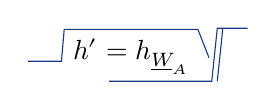
\begin{tikzpicture}[baseline=(fcue.base)]\node[inner sep=1pt] (fcue) {\ensuremath{h' = h_{\underline{W}_A}}};\draw[color=blue] ([xshift=-1.5em,yshift=-.4ex]fcue.west)--([xshift=-.3em,yshift=-.4ex]fcue.west)--([xshift=-.2em,yshift=.5ex]fcue.north west)--([xshift=.2em,yshift=.5ex]fcue.north east)--([xshift=.6em,yshift=-.1ex]fcue.east);\draw[color=blue] ([xshift=-.8em,yshift=-.3ex]fcue.south)--([xshift=.7em,yshift=-.3ex]fcue.south east)--([xshift=.9em,yshift=.6ex]fcue.north east)--([xshift=2em,yshift=.6ex]fcue.north east);\draw[color=blue] ([xshift=.9em,yshift=-.3ex]fcue.south east)--([xshift=1.1em,yshift=.6ex]fcue.north east);\end{tikzpicture}}{\[ h' = h_{\underline{W}_A} \]}{authorial display instruction}{ps_134-6_030-v0020} defined in terms of inter-% 
\margin{\tikz[baseline=(m.base)]{\node[inner sep=2pt] (m) {\shortstack{formule\\\`a la ligne}};\draw (m.center) ellipse (2.7em and 1.7em);}}
vals in $A^\wedge_{\mathrm{locas}}$\var{\deleted{\illegible{1}}}{}{deletion}{ps_134-6_030-v0021} ; \var{\inserted{this}}{\hand{this}}{insertion}{ps_134-6_030-v0022} \var{\deleted{which}}{}{deletion}{ps_134-6_030-v0023} depends a priori on the choice of $\underline{W}$ ,  as it
has to because th.1  gives a criterion for the functor i to be $M_a$-$\underline{W}$-%
aspheric which does depend on $\underline{W}$ . (\var{\over{i}{I}}{\hand{I}}{writing over}{ps_134-6_030-v0024}t surely wont be the same if we take
$\underline{W} = \underline{W}_\infty$  =  usual \var{\inserted[typed]{weak}}{weak}{typed insertion}{ps_134-6_030-v0025} equivalence,  or $\underline{W} = F\mathord{\rlap{\text{/}}l}(\mathrm{Cat})$  hence $\underline{W}_A = F\mathord{\rlap{\text{/}}l}(A)$  and

\margin{30}

% Visual collation: both supplied image halves inspected; see CHECK_DECISIONS_134_7_8.tsv.

%% END SOURCE ps_134-6_030
\ifnum\EditionMode=1
\psapparatusstart
\psentry{ps_134-6_030-v0001}{1}{writing over}{\over{em}{em}}{\hand{em}}{The superposed handwritten reading replaces the underlying reading.}
\psentry{ps_134-6_030-v0002}{2}{insertion}{\inserted{then}}{\hand{then}}{The handwritten insertion is incorporated at its indicated position; insertion brackets leave the running text.}
\psentry{ps_134-6_030-v0003}{3}{typed insertion}{\inserted[typed]{$\underline{W}$-}}{$\underline{W}$-}{The typed insertion is incorporated at its indicated position; insertion brackets leave the running text.}
\psentry{ps_134-6_030-v0004}{4}{typed insertion}{\inserted[typed]{$\underline{W}$-aspheric}}{$\underline{W}$-aspheric}{The typed insertion is incorporated at its indicated position; insertion brackets leave the running text.}
\psentry{ps_134-6_030-v0005}{5}{typewriter deletion}{\xout{\unsure{aspheric}}}{}{The typewriter strikes out this material; it leaves the corrected running text.}
\psentry{ps_134-6_030-v0006}{6}{typed insertion}{\inserted[typed]{strict $\underline{W}$-}}{strict $\underline{W}$-}{The typed insertion is incorporated at its indicated position; insertion brackets leave the running text.}
\psentry{ps_134-6_030-v0007}{7}{typewriter deletion}{\xout{local}}{}{The typewriter strikes out this material; it leaves the corrected running text.}
\psentry{ps_134-6_030-v0008}{8}{typewriter deletion}{\xout{in $M_c$}}{}{The typewriter strikes out this material; it leaves the corrected running text.}
\psentry{ps_134-6_030-v0009}{9}{typed insertion}{\inserted[typed]{distinct}}{distinct}{The typed insertion is incorporated at its indicated position; insertion brackets leave the running text.}
\psentry{ps_134-6_030-v0010}{10}{typewriter deletion}{\xout{equal}}{}{The typewriter strikes out this material; it leaves the corrected running text.}
\psentry{ps_134-6_030-v0011}{11}{typewriter deletion}{$\xout{\unsure{e}}$}{}{The typewriter strikes out this material; it leaves the corrected running text.}
\psentry{ps_134-6_030-v0012}{12}{writing over}{\over{s}{s}}{\hand{s}}{The superposed handwritten reading replaces the underlying reading.}
\psentry{ps_134-6_030-v0013}{13}{authorial spacing}{on\hand{/}page}{on page}{The pen divider separates the crowded words on and page. Preserve the stroke diplomatically and apply the visible spacing instruction in the reading.}
\psentry{ps_134-6_030-v0014}{14}{typewriter deletion}{\xout{r}}{}{The typewriter strikes out this material; it leaves the corrected running text.}
\psentry{ps_134-6_030-v0015}{15}{typewriter deletion}{\xout{assumptio}}{}{The typewriter strikes out this material; it leaves the corrected running text.}
\psentry{ps_134-6_030-v0016}{16}{typed insertion}{\inserted[typed]{trivial}}{trivial}{The typed insertion is incorporated at its indicated position; insertion brackets leave the running text.}
\psentry{ps_134-6_030-v0017}{17}{typewriter deletion}{\xout{contractibility s}}{}{The typewriter strikes out this material; it leaves the corrected running text.}
\psentry{ps_134-6_030-v0018}{18}{nonlexical marks}{\tikz[baseline=(ocue.base)]{\node[inner sep=0pt] (ocue) {o};\draw[color=blue] ([xshift=.3ex,yshift=.8ex]ocue.north) .. controls ([xshift=-.5ex]ocue.west) and ([xshift=-.2ex]ocue.south west) .. ([xshift=.2ex,yshift=-.2ex]ocue.south);}f}{of}{The source word of is clearly typed beneath an uninterpreted curved pen stroke. Omit only that graphic from the reading while preserving it diplomatically.}
\psentry{ps_134-6_030-v0019}{19}{deletion}{\deleted{thex}}{}{The author cancels this material by hand; it leaves the corrected running text.}
\psentry{ps_134-6_030-v0020}{20}{authorial display instruction}{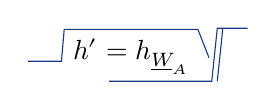
\begin{tikzpicture}[baseline=(fcue.base)]\node[inner sep=1pt] (fcue) {\ensuremath{h' = h_{\underline{W}_A}}};\draw[color=blue] ([xshift=-1.5em,yshift=-.4ex]fcue.west)--([xshift=-.3em,yshift=-.4ex]fcue.west)--([xshift=-.2em,yshift=.5ex]fcue.north west)--([xshift=.2em,yshift=.5ex]fcue.north east)--([xshift=.6em,yshift=-.1ex]fcue.east);\draw[color=blue] ([xshift=-.8em,yshift=-.3ex]fcue.south)--([xshift=.7em,yshift=-.3ex]fcue.south east)--([xshift=.9em,yshift=.6ex]fcue.north east)--([xshift=2em,yshift=.6ex]fcue.north east);\draw[color=blue] ([xshift=.9em,yshift=-.3ex]fcue.south east)--([xshift=1.1em,yshift=.6ex]fcue.north east);\end{tikzpicture}}{\[ h' = h_{\underline{W}_A} \]}{The circled formule a la ligne and bracketed formula request a separate displayed line. Preserve the original inline layout and marks diplomatically,then apply the requested display in the reading.}
\psentry{ps_134-6_030-v0021}{21}{deletion}{\deleted{\illegible{1}}}{}{The author cancels this material by hand; it leaves the corrected running text.}
\psentry{ps_134-6_030-v0022}{22}{insertion}{\inserted{this}}{\hand{this}}{The handwritten insertion is incorporated at its indicated position; insertion brackets leave the running text.}
\psentry{ps_134-6_030-v0023}{23}{deletion}{\deleted{which}}{}{The author cancels this material by hand; it leaves the corrected running text.}
\psentry{ps_134-6_030-v0024}{24}{writing over}{\over{i}{I}}{\hand{I}}{The superposed handwritten reading replaces the underlying reading.}
\psentry{ps_134-6_030-v0025}{25}{typed insertion}{\inserted[typed]{weak}}{weak}{The typed insertion is incorporated at its indicated position; insertion brackets leave the running text.}
\psapparatusend
\fi
\pssource{ps_134-6_031}{134-6/31}{https://grothendieck.umontpellier.fr/web/viewer.html?file=../134-6.pdf\#page=32}
\psnumber{ps_134-6_031-v0001}{1}
\psnumber{ps_134-6_031-v0002}{2}
\psnumber{ps_134-6_031-v0003}{3}
\psnumber{ps_134-6_031-v0004}{4}
\psnumber{ps_134-6_031-v0005}{5}
\psnumber{ps_134-6_031-v0006}{6}
\psnumber{ps_134-6_031-v0007}{7}
\psnumber{ps_134-6_031-v0008}{8}
\psnumber{ps_134-6_031-v0009}{9}
\psnumber{ps_134-6_031-v0010}{10}
\psnumber{ps_134-6_031-v0011}{11}
\psnumber{ps_134-6_031-v0012}{12}
\psnumber{ps_134-6_031-v0013}{13}
\psnumber{ps_134-6_031-v0014}{14}
\psnumber{ps_134-6_031-v0015}{15}
\psnumber{ps_134-6_031-v0016}{16}
\psnumber{ps_134-6_031-v0017}{17}
\psnumber{ps_134-6_031-v0018}{18}
\psnumber{ps_134-6_031-v0019}{19}
\psnumber{ps_134-6_031-v0020}{20}
\psnumber{ps_134-6_031-v0021}{21}
\psnumber{ps_134-6_031-v0022}{22}
\psnumber{ps_134-6_031-v0023}{23}
\psnumber{ps_134-6_031-v0024}{24}
\psnumber{ps_134-6_031-v0025}{25}
\psnumber{ps_134-6_031-v0026}{26}
\psnumber{ps_134-6_031-v0027}{27}
\psnumber{ps_134-6_031-v0028}{28}
\psnumber{ps_134-6_031-v0029}{29}
\psnumber{ps_134-6_031-v0030}{30}
\psnumber{ps_134-6_031-v0031}{31}
\psnumber{ps_134-6_031-v0032}{32}
\psnumber{ps_134-6_031-v0033}{33}
%% BEGIN SOURCE ps_134-6_031
% Pursuing Stacks (cotes 134-2 to 134-8): archive cote 134-6, site page 31 (PDF page 32), typescript page 349.
% typescript. Draft compared: ps5.tex:2869-2916.
% AI-transcribed by Claude Opus 5.5 (claude-opus-5-5, adaptive thinking, effort high), Message Batches API, batch ps3 (msgbatch_01XdFmuVVBAcgc7EFxdtCqsj), 2026-11-12; reviewed against both supplied scan halves; see CHECK_DECISIONS.tsv.
\scanpage{134-6/31}
\mspage{349}

the co\var{\over[typed]{j}{n}}{n}{typewriter overwriting}{ps_134-6_031-v0001}dition that i be $M_a$-$\underline{W}$-aspheric is always satisfied !\hand{)} However,
\var{\xout{when we}}{}{typewriter deletion}{ps_134-6_031-v0002}\var{\inserted[typed]{let's}}{let's}{typed insertion}{ps_134-6_031-v0003} assume A to be totally $\underline{W}$-aspheric and every object of A has a
section(over the final object $e_{A^{\wedge}}$ of $A^{\wedge}$ ) \var{\over{o}{o}}{\hand{o}}{writing over}{ps_134-6_031-v0004}\var{\over{r}{r}}{\hand{r}}{writing over}{ps_134-6_031-v0005}, what amounts to the
same, every``non-empty\var{''\hand{/}object}{'' object}{authorial spacing}{ps_134-6_031-v0006} of $A^{\wedge}$ has a section - \var{\xout{these conditions}}{}{typewriter deletion}{ps_134-6_031-v0007}
\var{\xout{in fact}}{}{typewriter deletion}{ps_134-6_031-v0008} we'll say in this case A is ``\uline{strictly} \var{\xout{$\underline{W}$ asph}}{}{typewriter deletion}{ps_134-6_031-v0009} \uline{totally $\underline{W}$-aspheric}\hand{''}
(compare section 60, p.149 , in the particular case $\underline{W} = \underline{W}_{\infty}$ , and
with $A^{\wedge}$ replaced by an arbitrary topos). Let's assume moreover that
$\underline{W}$ satisfies Loc 4) . In this case, the homotopy structure $h' = h_{\underline{W}_A}$
does not depend on the choice of $\underline{W}$ , namely it is the so-called
``canonical'' homotopy structure'' \var{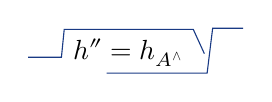
\begin{tikzpicture}[baseline=(fcue.base)]\node[inner sep=1pt] (fcue) {\ensuremath{h'' = h_{A^{\wedge}}}};\draw[color=blue] ([xshift=-1.5em,yshift=-.4ex]fcue.west)--([xshift=-.3em,yshift=-.4ex]fcue.west)--([xshift=-.2em,yshift=.5ex]fcue.north west)--([xshift=.2em,yshift=.5ex]fcue.north east)--([xshift=.6em,yshift=-.1ex]fcue.east);\draw[color=blue] ([xshift=-.8em,yshift=-.3ex]fcue.south)--([xshift=.7em,yshift=-.3ex]fcue.south east)--([xshift=.9em,yshift=.6ex]fcue.north east)--([xshift=2em,yshift=.6ex]fcue.north east);\end{tikzpicture}}{\[ h'' = h_{A^{\wedge}} \]}{probable authorial display instruction}{ps_134-6_031-v0010} of the \var{\inserted[typed]{strictly}}{strictly}{typed insertion}{ps_134-6_031-v0011} (totally 0-connected)
categ\var{\over[typed]{b}{o}}{o}{typewriter overwriting}{ps_134-6_031-v0012}ry $A^{\wedge}$ (cf. section 57), which in the special \var{\over[typed]{\illegible{1}}{c}}{c}{typewriter overwriting}{ps_134-6_031-v0013}\var{\over[typed]{i}{a}}{a}{typewriter overwriting}{ps_134-6_031-v0014}se of a category
$A^{\wedge}$ can also be defined as the homotopy structure $h_{\underline{W}_o\hand{A}}$ associated to
$\underline{W}_o\hand{A}$, where $\underline{W}_o$ is the coar\var{\over[typed]{\illegible{1}}{s}}{s}{typewriter overwriting}{ps_134-6_031-v0015}est \var{\over[typed]{v}{b}}{b}{typewriter overwriting}{ps_134-6_031-v0016}asic localizer satisfying Loc 4) i.e.
\[ \underline{W}_o = \hand{\{} f \hand{\in} \mathrm{Fl}(\mathrm{Cat}) \hand{|} \hand{\pi}_o(f) \text{ bijective}\hand{\}} \quad . \]
T\var{\over[typed]{h}{h}}{h}{typewriter overwriting}{ps_134-6_031-v0017}e proof of this fact \var{\xout{is essentially the same as}}{}{typewriter deletion}{ps_134-6_031-v0018} $h' = h''$ i.e.
\[ h_{\underline{W}_A} = h_{A^{\wedge}} \quad ( = h_{\underline{W}_o} ) \]
is essentially the \var{\over[typed]{\illegible{1}}{s}}{s}{typewriter overwriting}{ps_134-6_031-v0019}ame as for the s\var{\over[typed]{\illegible{1}}{m}}{m}{typewriter overwriting}{ps_134-6_031-v0020}iliar prop. (section 60, p.149),
The condition L\var{\over[typed]{o}{o}}{o}{typewriter overwriting}{ps_134-6_031-v0021}c 4) on $\underline{W}$ i.e. $\underline{W} \hand{\subset} \underline{W}_o$ clearly implies
\[ h_{\underline{W}_A} \hand{\subset} h_{\underline{W}_o\hand{A}} \quad , \]
and to get the opposite inequality, for which we'll use the assumption
on A , we only have to prove that for any 0-connected object X of $A^{\wedge}$,
any two sections are $(h'=h_{\underline{W}_A}$ )-homotopic, a fortiori ( as $h \hand{\leq} h'$
by the assumption of total $\underline{W}$-asphericity of A) it is enough to prove
they are h-homotopic. Now this \var{\deleted{follows from the following easy result}}{}{deletion}{ps_134-6_031-v0022}
\var{\deleted{applied to \quad $= A^{\wedge}$ (and which implies equally the proposition of secti-}}{}{deletion}{ps_134-6_031-v0023}%
\var{\deleted{on 60 cited above).}}{}{deletion}{ps_134-6_031-v0024} \var{\inserted{\deleted{is stated} follows from lemma 2 p.268, applied
to $\mathcal{C} = A^{\wedge}$, $C = A$.}}{\hand{ follows from lemma 2 p.268, applied
to $\mathcal{C} = A^{\wedge}$, $C = A$.}}{insertion}{ps_134-6_031-v0025}

\var{\deleted{\uline{Proposition} 4. Let \quad be a topos, A a full generating subcategory}}{}{deletion}{ps_134-6_031-v0026}
\var{\deleted{of \quad , made up with 0-connected objects. We assume \quad totally 0-}}{}{deletion}{ps_134-6_031-v0027}
\var{\deleted{connected or (what amounts to the same) that the product of any two}}{}{deletion}{ps_134-6_031-v0028}
\var{\deleted{objects in A is 0-connected, and moreover that any``non-empty'' object}}{}{deletion}{ps_134-6_031-v0029}
\var{\deleted{of \quad has a section (again it is enough to check this for the objects}}{}{deletion}{ps_134-6_031-v0030}
\var{\deleted{in A). Then the canonical homotopy structure h of \quad (defined in}}{}{deletion}{ps_134-6_031-v0031}
\var{\deleted{terms of intervals which are 0-connected as a generating family of}}{}{deletion}{ps_134-6_031-v0032}
\var{\deleted{homotopy intervals) is equal to the homotopy structure \inserted{$h$} generated}}{}{deletion}{ps_134-6_031-v0033}

\margin{31}

% Visual collation: both supplied image halves inspected; see CHECK_DECISIONS_134_7_8.tsv.

%% END SOURCE ps_134-6_031
\ifnum\EditionMode=1
\psapparatusstart
\psentry{ps_134-6_031-v0001}{1}{typewriter overwriting}{\over[typed]{j}{n}}{n}{The superposed typed reading replaces the underlying reading.}
\psentry{ps_134-6_031-v0002}{2}{typewriter deletion}{\xout{when we}}{}{The typewriter strikes out this material; it leaves the corrected running text.}
\psentry{ps_134-6_031-v0003}{3}{typed insertion}{\inserted[typed]{let's}}{let's}{The typed insertion is incorporated at its indicated position; insertion brackets leave the running text.}
\psentry{ps_134-6_031-v0004}{4}{writing over}{\over{o}{o}}{\hand{o}}{The superposed handwritten reading replaces the underlying reading.}
\psentry{ps_134-6_031-v0005}{5}{writing over}{\over{r}{r}}{\hand{r}}{The superposed handwritten reading replaces the underlying reading.}
\psentry{ps_134-6_031-v0006}{6}{authorial spacing}{''\hand{/}object}{'' object}{The pen divider separates the closing quotation marks from object.}
\psentry{ps_134-6_031-v0007}{7}{typewriter deletion}{\xout{these conditions}}{}{The typewriter strikes out this material; it leaves the corrected running text.}
\psentry{ps_134-6_031-v0008}{8}{typewriter deletion}{\xout{in fact}}{}{The typewriter strikes out this material; it leaves the corrected running text.}
\psentry{ps_134-6_031-v0009}{9}{typewriter deletion}{\xout{$\underline{W}$ asph}}{}{The typewriter strikes out this material; it leaves the corrected running text.}
\psentry{ps_134-6_031-v0010}{10}{probable authorial display instruction}{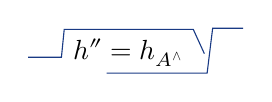
\begin{tikzpicture}[baseline=(fcue.base)]\node[inner sep=1pt] (fcue) {\ensuremath{h'' = h_{A^{\wedge}}}};\draw[color=blue] ([xshift=-1.5em,yshift=-.4ex]fcue.west)--([xshift=-.3em,yshift=-.4ex]fcue.west)--([xshift=-.2em,yshift=.5ex]fcue.north west)--([xshift=.2em,yshift=.5ex]fcue.north east)--([xshift=.6em,yshift=-.1ex]fcue.east);\draw[color=blue] ([xshift=-.8em,yshift=-.3ex]fcue.south)--([xshift=.7em,yshift=-.3ex]fcue.south east)--([xshift=.9em,yshift=.6ex]fcue.north east)--([xshift=2em,yshift=.6ex]fcue.north east);\end{tikzpicture}}{\[ h'' = h_{A^{\wedge}} \]}{The stepped brackets match the preceding page cue explicitly labelled formule a la ligne;the display interpretation is a recorded contextual inference.}
\psentry{ps_134-6_031-v0011}{11}{typed insertion}{\inserted[typed]{strictly}}{strictly}{The typed insertion is incorporated at its indicated position; insertion brackets leave the running text.}
\psentry{ps_134-6_031-v0012}{12}{typewriter overwriting}{\over[typed]{b}{o}}{o}{The superposed typed reading replaces the underlying reading.}
\psentry{ps_134-6_031-v0013}{13}{typewriter overwriting}{\over[typed]{\illegible{1}}{c}}{c}{The superposed typed reading replaces the underlying reading.}
\psentry{ps_134-6_031-v0014}{14}{typewriter overwriting}{\over[typed]{i}{a}}{a}{The superposed typed reading replaces the underlying reading.}
\psentry{ps_134-6_031-v0015}{15}{typewriter overwriting}{\over[typed]{\illegible{1}}{s}}{s}{The superposed typed reading replaces the underlying reading.}
\psentry{ps_134-6_031-v0016}{16}{typewriter overwriting}{\over[typed]{v}{b}}{b}{The superposed typed reading replaces the underlying reading.}
\psentry{ps_134-6_031-v0017}{17}{typewriter overwriting}{\over[typed]{h}{h}}{h}{The superposed typed reading replaces the underlying reading.}
\psentry{ps_134-6_031-v0018}{18}{typewriter deletion}{\xout{is essentially the same as}}{}{The typewriter strikes out this material; it leaves the corrected running text.}
\psentry{ps_134-6_031-v0019}{19}{typewriter overwriting}{\over[typed]{\illegible{1}}{s}}{s}{The superposed typed reading replaces the underlying reading.}
\psentry{ps_134-6_031-v0020}{20}{typewriter overwriting}{\over[typed]{\illegible{1}}{m}}{m}{The superposed typed reading replaces the underlying reading.}
\psentry{ps_134-6_031-v0021}{21}{typewriter overwriting}{\over[typed]{o}{o}}{o}{The superposed typed reading replaces the underlying reading.}
\psentry{ps_134-6_031-v0022}{22}{deletion}{\deleted{follows from the following easy result}}{}{The author cancels this material by hand; it leaves the corrected running text.}
\psentry{ps_134-6_031-v0023}{23}{deletion}{\deleted{applied to \quad $= A^{\wedge}$ (and which implies equally the proposition of secti-}}{}{The author cancels this material by hand; it leaves the corrected running text.}
\psentry{ps_134-6_031-v0024}{24}{deletion}{\deleted{on 60 cited above).}}{}{The author cancels this material by hand; it leaves the corrected running text.}
\psentry{ps_134-6_031-v0025}{25}{insertion}{\inserted{\deleted{is stated} follows from lemma 2 p.268, applied
to $\mathcal{C} = A^{\wedge}$, $C = A$.}}{\hand{ follows from lemma 2 p.268, applied
to $\mathcal{C} = A^{\wedge}$, $C = A$.}}{The handwritten insertion is incorporated at its indicated position; insertion brackets leave the running text.}
\psentry{ps_134-6_031-v0026}{26}{deletion}{\deleted{\uline{Proposition} 4. Let \quad be a topos, A a full generating subcategory}}{}{The author cancels this material by hand; it leaves the corrected running text.}
\psentry{ps_134-6_031-v0027}{27}{deletion}{\deleted{of \quad , made up with 0-connected objects. We assume \quad totally 0-}}{}{The author cancels this material by hand; it leaves the corrected running text.}
\psentry{ps_134-6_031-v0028}{28}{deletion}{\deleted{connected or (what amounts to the same) that the product of any two}}{}{The author cancels this material by hand; it leaves the corrected running text.}
\psentry{ps_134-6_031-v0029}{29}{deletion}{\deleted{objects in A is 0-connected, and moreover that any``non-empty'' object}}{}{The author cancels this material by hand; it leaves the corrected running text.}
\psentry{ps_134-6_031-v0030}{30}{deletion}{\deleted{of \quad has a section (again it is enough to check this for the objects}}{}{The author cancels this material by hand; it leaves the corrected running text.}
\psentry{ps_134-6_031-v0031}{31}{deletion}{\deleted{in A). Then the canonical homotopy structure h of \quad (defined in}}{}{The author cancels this material by hand; it leaves the corrected running text.}
\psentry{ps_134-6_031-v0032}{32}{deletion}{\deleted{terms of intervals which are 0-connected as a generating family of}}{}{The author cancels this material by hand; it leaves the corrected running text.}
\psentry{ps_134-6_031-v0033}{33}{deletion}{\deleted{homotopy intervals) is equal to the homotopy structure \inserted{$h$} generated}}{}{The author cancels this material by hand; it leaves the corrected running text.}
\psapparatusend
\fi
\pssource{ps_134-6_032}{134-6/32}{https://grothendieck.umontpellier.fr/web/viewer.html?file=../134-6.pdf\#page=33}
\psnumber{ps_134-6_032-v0001}{1}
\psnumber{ps_134-6_032-v0002}{2}
\psnumber{ps_134-6_032-v0003}{3}
\psnumber{ps_134-6_032-v0004}{4}
\psnumber{ps_134-6_032-v0005}{5}
\psnumber{ps_134-6_032-v0006}{6}
\psnumber{ps_134-6_032-v0007}{7}
\psnumber{ps_134-6_032-v0008}{8}
\psnumber{ps_134-6_032-v0009}{9}
\psnumber{ps_134-6_032-v0010}{10}
\psnumber{ps_134-6_032-v0011}{11}
\psnumber{ps_134-6_032-v0012}{12}
\psnumber{ps_134-6_032-v0013}{13}
\psnumber{ps_134-6_032-v0014}{14}
\psnumber{ps_134-6_032-v0015}{15}
%% BEGIN SOURCE ps_134-6_032
% Pursuing Stacks (cotes 134-2 to 134-8): archive cote 134-6, site page 32 (PDF page 33), typescript page 350.
% typescript. Draft compared: ps5.tex:2901-2973.
% AI-transcribed by Claude Opus 5.5 (claude-opus-5-5, adaptive thinking, effort high), Message Batches API, batch ps3 (msgbatch_01XdFmuVVBAcgc7EFxdtCqsj), 2026-11-12; reviewed against both supplied scan halves; see CHECK_DECISIONS.tsv.
\scanpage{134-6/32}
\mspage{350}

\var{\xout{We now can prove the foll}}{}{typewriter deletion}{ps_134-6_032-v0001}
The preceding reflections thus prove the following afterthought to
theorem 1 of section 79 :

\var{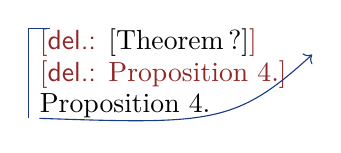
\begin{tikzpicture}[baseline=(ph.base)]\node[inner sep=0pt] (ph) {\deleted{\uline{Proposition} 4.}};\node[anchor=south west,inner sep=0pt] (pt) at ([yshift=.3ex]ph.north west) {\deleted{\hand{\unsure{Theorem}}}};\node[anchor=north west,inner sep=0pt] (pb) at ([yshift=-.3ex]ph.south west) {\hand{Proposition 4.}};\draw[color=blue] ([xshift=-.4em]pb.south west)--([xshift=-.4em]pt.north west)--([xshift=.4em]pt.north west);\draw[color=blue,->] (pb.south west) .. controls ([yshift=-.5ex]pb.south east) and ([xshift=.9em,yshift=-.5ex]pb.south east) .. ([xshift=.9em,yshift=.5ex]ph.north east);\end{tikzpicture}}{\hand{Proposition 4.}}{heading revision}{ps_134-6_032-v0002} Let $(M,M_c)$ be a contractibility structure, $A$ a small
category, $i\colon A\hand{\longrightarrow} M$ a functor factoring through $M_c$ . \var{\xout{We assume}}{}{typewriter deletion}{ps_134-6_032-v0003} Let
moreover $\underline{W}$ be a basic localizer satisfying L\var{\tikz[baseline=(lo.base)]{\node[inner sep=0pt] (lo) {o};\draw ([xshift=-.4ex,yshift=.7ex]lo.north) .. controls ([yshift=-.1ex]lo.north) .. ([xshift=.4ex,yshift=.7ex]lo.north);\draw ([xshift=-.4ex,yshift=-.8ex]lo.south) .. controls ([yshift=.2ex]lo.south) .. ([xshift=.4ex,yshift=-.8ex]lo.south);}}{o}{nonlexical marks}{ps_134-6_032-v0004}c 4) . We assume $A$
\var{\xout{totally W}}{}{typewriter deletion}{ps_134-6_032-v0005} \uline{strictly totally $\underline{W}$-aspheric}, i.e. totally $\underline{W}$-aspheric and
moreover any object of $A$ has a section (over $e_{A^\wedge}$) .

a) The homotopy structure $h_{\underline{W}_A}$ on $A^\wedge$ is equal to the canonical
homotopy structure $h_{A^\wedge}$ defined by 0-connected intervals, and equal
also to the homotopy structure $h$ defined by intervals coming from $A$ :
\[ (6) \qquad h = h_{\underline{W}_A} = h_{A^\wedge} \ . \]
In what follows, we assume $A^\wedge$ endowed with this homotopy structure,
and denote by $A^\wedge_c$ the set of all contractible objects in $A^\wedge$. We equal-%
ly endow $A^\wedge$ with it's canonical $\underline{W}$-asphericity structure , and $M$ with
the $\underline{W}$-asphericity structure associated to it's contractibility struc-%
ture $M_c$ . With these conventions:

b) T\var{\over[typed]{h}{h}}{h}{typewriter overwriting}{ps_134-6_032-v0006}e following conditions on $i$ are equivalent, where
\[ i^* : M \hand{\longrightarrow} A^\wedge \]
is the functor defined as usual in terms of $i$:

(i) $i^*$ is compatible with the homotopy structures (cf. criteria on
pages 251-252), which can be expressed also by
\[ i^*(M_c) \hand{\subset} A^\wedge_c \]
(a condition undependent from $\underline{W}$\hand{,} in view of a)).

(ii) $i$ is $\underline{W}$-aspheric , i.e.
\[ \var{\xout{\illegible{1}}}{}{typewriter deletion}{ps_134-6_032-v0007}M_{\underline{W}} \var{\over{\illegible{1}}{\subset}}{\hand{\subset}}{writing over}{ps_134-6_032-v0008}\hand{(i^*)^{-1}}\hand{(}A^\wedge_{\underline{W}}) \ , \]
(where $M_{\underline{W}}$ and $A^\wedge_{\underline{W}}$ are the sets of \var{\inserted{$\underline{W}$-}}{\hand{$\underline{W}$-}}{insertion}{ps_134-6_032-v0009} aspheric objects in $M$ and \var{\inserted[typed]{in $A^\wedge$).}}{in $A^\wedge$).}{typed insertion}{ps_134-6_032-v0010}

(iii) (F\var{\over[typed]{o}{o}}{o}{typewriter overwriting}{ps_134-6_032-v0011}r a given full subcategory \var{\inserted{$C$}}{\hand{$C$}}{insertion}{ps_134-6_032-v0012} of $M$ generating the contracti-%
bility structure $M_c$):
\[ i^*(C) \hand{\subset} A^\wedge_{\underline{W}_o} = \text{set of 0-connected objects of } \var{\inserted[typed]{A^\wedge.}}{A^\wedge.}{typed insertion}{ps_134-6_032-v0013} \]

c) Assume these conditions hold, and moreover that the contrac-%
tibility structure \var{\xout{$\unsure{M_c}$}}{}{typewriter deletion}{ps_134-6_032-v0014}\hand{of} $M$ is non trivial. T\var{\over[typed]{h}{h}}{h}{typewriter overwriting}{ps_134-6_032-v0015}en $A$ is a strict $\underline{W}$-test
category.

\margin{32}

% Visual collation: both supplied image halves inspected; see CHECK_DECISIONS_134_7_8.tsv.

%% END SOURCE ps_134-6_032
\ifnum\EditionMode=1
\psapparatusstart
\psentry{ps_134-6_032-v0001}{1}{typewriter deletion}{\xout{We now can prove the foll}}{}{The typewriter strikes out this material; it leaves the corrected running text.}
\psentry{ps_134-6_032-v0002}{2}{heading revision}{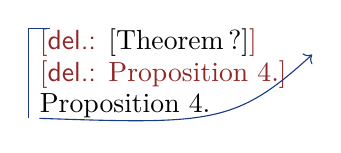
\begin{tikzpicture}[baseline=(ph.base)]\node[inner sep=0pt] (ph) {\deleted{\uline{Proposition} 4.}};\node[anchor=south west,inner sep=0pt] (pt) at ([yshift=.3ex]ph.north west) {\deleted{\hand{\unsure{Theorem}}}};\node[anchor=north west,inner sep=0pt] (pb) at ([yshift=-.3ex]ph.south west) {\hand{Proposition 4.}};\draw[color=blue] ([xshift=-.4em]pb.south west)--([xshift=-.4em]pt.north west)--([xshift=.4em]pt.north west);\draw[color=blue,->] (pb.south west) .. controls ([yshift=-.5ex]pb.south east) and ([xshift=.9em,yshift=-.5ex]pb.south east) .. ([xshift=.9em,yshift=.5ex]ph.north east);\end{tikzpicture}}{\hand{Proposition 4.}}{The lower handwritten heading replaces the cancelled typed heading and the cancelled tentative upper word. The reading applies that visible replacement and omits its placement strokes.}
\psentry{ps_134-6_032-v0003}{3}{typewriter deletion}{\xout{We assume}}{}{The typewriter strikes out this material; it leaves the corrected running text.}
\psentry{ps_134-6_032-v0004}{4}{nonlexical marks}{\tikz[baseline=(lo.base)]{\node[inner sep=0pt] (lo) {o};\draw ([xshift=-.4ex,yshift=.7ex]lo.north) .. controls ([yshift=-.1ex]lo.north) .. ([xshift=.4ex,yshift=.7ex]lo.north);\draw ([xshift=-.4ex,yshift=-.8ex]lo.south) .. controls ([yshift=.2ex]lo.south) .. ([xshift=.4ex,yshift=-.8ex]lo.south);}}{o}{The live o is clear;the unassigned upper/lower arcs have no secure additional lexical reading.}
\psentry{ps_134-6_032-v0005}{5}{typewriter deletion}{\xout{totally W}}{}{The typewriter strikes out this material; it leaves the corrected running text.}
\psentry{ps_134-6_032-v0006}{6}{typewriter overwriting}{\over[typed]{h}{h}}{h}{The superposed typed reading replaces the underlying reading.}
\psentry{ps_134-6_032-v0007}{7}{typewriter deletion}{$\xout{\illegible{1}}$}{}{The typewriter strikes out this material; it leaves the corrected running text.}
\psentry{ps_134-6_032-v0008}{8}{writing over}{$\over{\illegible{1}}{\subset}$}{$\hand{\subset}$}{The superposed handwritten reading replaces the underlying reading.}
\psentry{ps_134-6_032-v0009}{9}{insertion}{\inserted{$\underline{W}$-}}{\hand{$\underline{W}$-}}{The handwritten insertion is incorporated at its indicated position; insertion brackets leave the running text.}
\psentry{ps_134-6_032-v0010}{10}{typed insertion}{\inserted[typed]{in $A^\wedge$).}}{in $A^\wedge$).}{The typed insertion is incorporated at its indicated position; insertion brackets leave the running text.}
\psentry{ps_134-6_032-v0011}{11}{typewriter overwriting}{\over[typed]{o}{o}}{o}{The superposed typed reading replaces the underlying reading.}
\psentry{ps_134-6_032-v0012}{12}{insertion}{\inserted{$C$}}{\hand{$C$}}{The handwritten insertion is incorporated at its indicated position; insertion brackets leave the running text.}
\psentry{ps_134-6_032-v0013}{13}{typed insertion}{$\inserted[typed]{A^\wedge.}$}{$A^\wedge.$}{The typed insertion is incorporated at its indicated position; insertion brackets leave the running text.}
\psentry{ps_134-6_032-v0014}{14}{typewriter deletion}{\xout{$\unsure{M_c}$}}{}{The typewriter strikes out this material; it leaves the corrected running text.}
\psentry{ps_134-6_032-v0015}{15}{typewriter overwriting}{\over[typed]{h}{h}}{h}{The superposed typed reading replaces the underlying reading.}
\psapparatusend
\fi
\pssource{ps_134-6_033}{134-6/33}{https://grothendieck.umontpellier.fr/web/viewer.html?file=../134-6.pdf\#page=34}
\psnumber{ps_134-6_033-v0001}{1}
\psnumber{ps_134-6_033-v0002}{2}
\psnumber{ps_134-6_033-v0003}{3}
\psnumber{ps_134-6_033-v0004}{4}
\psnumber{ps_134-6_033-v0005}{5}
\psnumber{ps_134-6_033-v0006}{6}
\psnumber{ps_134-6_033-v0007}{7}
\psnumber{ps_134-6_033-v0008}{8}
\psnumber{ps_134-6_033-v0009}{9}
\psnumber{ps_134-6_033-v0010}{10}
\psnumber{ps_134-6_033-v0011}{11}
\psnumber{ps_134-6_033-v0012}{12}
\psnumber{ps_134-6_033-v0013}{13}
\psnumber{ps_134-6_033-v0014}{14}
\psnumber{ps_134-6_033-v0015}{15}
\psnumber{ps_134-6_033-v0016}{16}
\psnumber{ps_134-6_033-v0017}{17}
\psnumber{ps_134-6_033-v0018}{18}
\psnumber{ps_134-6_033-v0019}{19}
%% BEGIN SOURCE ps_134-6_033
% Pursuing Stacks (cotes 134-2 to 134-8): archive cote 134-6, site page 33 (PDF page 34), typescript page 351.
% typescript. Draft compared: ps5.tex:2956-3029.
% AI-transcribed by Claude Opus 5.5 (claude-opus-5-5, adaptive thinking, effort high), Message Batches API, batch ps3 (msgbatch_01XdFmuVVBAcgc7EFxdtCqsj), 2026-11-12; reviewed against both supplied scan halves; see CHECK_DECISIONS.tsv.
\scanpage{134-6/33}
\mspage{351}

Proof. Part a) has been proved in remark 2 above, and in view of
th. 1 \var{\xout{p.252 cor.1}}{}{typewriter deletion}{ps_134-6_033-v0001} p.252 , the equivalence of (i) and (ii) is clear,
hence also the equivalence with (iii) by applying loc. cit. to $\underline{W}_o$
instead of $\underline{W}$ . Part c) now follows from prop.3 cor. 1 b).

\uline{Corollary}. Under the conditions of c) above, if $M_c$ is \var{\inserted[typed]{$\underline{W}$-}}{$\underline{W}$-}{typed insertion}{ps_134-6_033-v0002}modelizing,
then i is a $\underline{W}$-test functor, and induces an \uline{equivalence}
\[ \mathrm{Hot}_{M,\underline{W}} \overset{\hand{def}}{=} \underline{W}_M^{\ -1} M \ \hand{\xrightarrow{\approx}}\var{\xout{\illegible{2}}}{}{typewriter deletion}{ps_134-6_033-v0003}\ \mathrm{Hot}_{A,\underline{W}} \overset{\hand{def}}{=} \underline{W}_A^{\ -1}A\hat{\ } . \]

8.7.

96. Yesterday's notes have proceeded very falteringly, to my sur-%
prise, while everything seemed ready for smooth \var{\xout{exposition}}{}{typewriter deletion}{ps_134-6_033-v0004}\var{\inserted[typed]{sailing}}{sailing}{typed insertion}{ps_134-6_033-v0005}. A number
of times,\var{\xout{I}}{}{typewriter deletion}{ps_134-6_033-v0006} after going on for a page or two``following my nose'' (as
they say in German), or for half a page, it turned out it just was'%
nt right that way and I would \var{\xout{put}}{}{typewriter deletion}{ps_134-6_033-v0007} feel quite stupid and put the silly
pages away as scratchpaper and \var{\xout{do it}}{}{typewriter deletion}{ps_134-6_033-v0008} have another start. THere would'%
nt have been any point dragging the poor reader (if there is still one
left ...) along on my stumbling path, where it was a matter merely of
getting some technical adjustments right. Maybe it is just that atten-%
tion was distracted, perhaps precisely through this (partly mistaken,
and anyhow not too inspiring) feeling that everything was kind of
cooked already, and what was left to do was just swallow ! What came
out in the process was that finally things were not so clear yet in my
mind as I \var{\xout{expected}}{}{typewriter deletion}{ps_134-6_033-v0009} thought they were. It is a frequent experience
that whenever one wants to go ahead too quic\var{\over[typed]{\illegible{1}}{k}}{k}{typewriter overwriting}{ps_134-6_033-v0010}ly, one finds oneself
dispersing stupidly a hell of a lot of energy ...

T\var{\over[typed]{h}{h}}{h}{typewriter overwriting}{ps_134-6_033-v0011}ere occured to me some unadequacies with terminology. O\var{\over[typed]{n}{n}}{n}{typewriter overwriting}{ps_134-6_033-v0012}e is
about the property of certain categories (contractors or precontractors
for instance) that every object of A has a section (over $e_{A\hat{\ }}$ ), which
can be viewed also as a property of the topos $A\hat{\ }=\hand{\mathcal{A}}$, namely that any
``non empty'' object of the topos has a section. This is immediately
seen \var{\xout{as being equivalent}}{}{typewriter deletion}{ps_134-6_033-v0013} (for any given topos \hand{$\mathcal{A}$}) \var{\xout{to}}{}{typewriter deletion}{ps_134-6_033-v0014}\var{\inserted[typed]{to imply}}{to imply}{typed insertion}{ps_134-6_033-v0015} the property that
the final object $e_{\hand{\mathcal{A}}}$ has only the two trivial subobjects, the ``empty''
and the ``full'' one - or equivalently, that any subtopos of the
topos is either the e\var{\over[typed]{p}{m}}{m}{typewriter overwriting}{ps_134-6_033-v0016}pty or the full one, \var{\xout{\unsure{This is}}}{}{typewriter deletion}{ps_134-6_033-v0017}\var{\inserted[typed]{- a property, too ,}}{- a property, too ,}{typed insertion}{ps_134-6_033-v0018} of obvious
geometric significance . In case of a topos of the type A\^{}, one im-%
mediately sees the two properties are equivalent - but this is not \var{\xout{tr}}{}{typewriter deletion}{ps_134-6_033-v0019}

\margin{33}

% Visual collation: both supplied image halves inspected; see CHECK_DECISIONS_134_7_8.tsv.

%% END SOURCE ps_134-6_033
\ifnum\EditionMode=1
\psapparatusstart
\psentry{ps_134-6_033-v0001}{1}{typewriter deletion}{\xout{p.252 cor.1}}{}{The typewriter strikes out this material; it leaves the corrected running text.}
\psentry{ps_134-6_033-v0002}{2}{typed insertion}{\inserted[typed]{$\underline{W}$-}}{$\underline{W}$-}{The typed insertion is incorporated at its indicated position; insertion brackets leave the running text.}
\psentry{ps_134-6_033-v0003}{3}{typewriter deletion}{$\xout{\illegible{2}}$}{}{The typewriter strikes out this material; it leaves the corrected running text.}
\psentry{ps_134-6_033-v0004}{4}{typewriter deletion}{\xout{exposition}}{}{The typewriter strikes out this material; it leaves the corrected running text.}
\psentry{ps_134-6_033-v0005}{5}{typed insertion}{\inserted[typed]{sailing}}{sailing}{The typed insertion is incorporated at its indicated position; insertion brackets leave the running text.}
\psentry{ps_134-6_033-v0006}{6}{typewriter deletion}{\xout{I}}{}{The typewriter strikes out this material; it leaves the corrected running text.}
\psentry{ps_134-6_033-v0007}{7}{typewriter deletion}{\xout{put}}{}{The typewriter strikes out this material; it leaves the corrected running text.}
\psentry{ps_134-6_033-v0008}{8}{typewriter deletion}{\xout{do it}}{}{The typewriter strikes out this material; it leaves the corrected running text.}
\psentry{ps_134-6_033-v0009}{9}{typewriter deletion}{\xout{expected}}{}{The typewriter strikes out this material; it leaves the corrected running text.}
\psentry{ps_134-6_033-v0010}{10}{typewriter overwriting}{\over[typed]{\illegible{1}}{k}}{k}{The superposed typed reading replaces the underlying reading.}
\psentry{ps_134-6_033-v0011}{11}{typewriter overwriting}{\over[typed]{h}{h}}{h}{The superposed typed reading replaces the underlying reading.}
\psentry{ps_134-6_033-v0012}{12}{typewriter overwriting}{\over[typed]{n}{n}}{n}{The superposed typed reading replaces the underlying reading.}
\psentry{ps_134-6_033-v0013}{13}{typewriter deletion}{\xout{as being equivalent}}{}{The typewriter strikes out this material; it leaves the corrected running text.}
\psentry{ps_134-6_033-v0014}{14}{typewriter deletion}{\xout{to}}{}{The typewriter strikes out this material; it leaves the corrected running text.}
\psentry{ps_134-6_033-v0015}{15}{typed insertion}{\inserted[typed]{to imply}}{to imply}{The typed insertion is incorporated at its indicated position; insertion brackets leave the running text.}
\psentry{ps_134-6_033-v0016}{16}{typewriter overwriting}{\over[typed]{p}{m}}{m}{The superposed typed reading replaces the underlying reading.}
\psentry{ps_134-6_033-v0017}{17}{typewriter deletion}{\xout{\unsure{This is}}}{}{The typewriter strikes out this material; it leaves the corrected running text.}
\psentry{ps_134-6_033-v0018}{18}{typed insertion}{\inserted[typed]{- a property, too ,}}{- a property, too ,}{The typed insertion is incorporated at its indicated position; insertion brackets leave the running text.}
\psentry{ps_134-6_033-v0019}{19}{typewriter deletion}{\xout{tr}}{}{The typewriter strikes out this material; it leaves the corrected running text.}
\psapparatusend
\fi
\pssource{ps_134-6_034}{134-6/34}{https://grothendieck.umontpellier.fr/web/viewer.html?file=../134-6.pdf\#page=35}
\psnumber{ps_134-6_034-v0001}{1}
\psnumber{ps_134-6_034-v0002}{2}
\psnumber{ps_134-6_034-v0003}{3}
\psnumber{ps_134-6_034-v0004}{4}
\psnumber{ps_134-6_034-v0005}{5}
\psnumber{ps_134-6_034-v0006}{6}
\psnumber{ps_134-6_034-v0007}{7}
\psnumber{ps_134-6_034-v0008}{8}
\psnumber{ps_134-6_034-v0009}{9}
\psnumber{ps_134-6_034-v0010}{10}
\psnumber{ps_134-6_034-v0011}{11}
\psnumber{ps_134-6_034-v0012}{12}
\psnumber{ps_134-6_034-v0013}{13}
\psnumber{ps_134-6_034-v0014}{14}
\psnumber{ps_134-6_034-v0015}{15}
\psnumber{ps_134-6_034-v0016}{16}
\psnumber{ps_134-6_034-v0017}{17}
\psnumber{ps_134-6_034-v0018}{18}
\psnumber{ps_134-6_034-v0019}{19}
\psnumber{ps_134-6_034-v0020}{20}
\psnumber{ps_134-6_034-v0021}{21}
\psnumber{ps_134-6_034-v0022}{22}
\psnumber{ps_134-6_034-v0023}{23}
\psnumber{ps_134-6_034-v0024}{24}
%% BEGIN SOURCE ps_134-6_034
% Pursuing Stacks (cotes 134-2 to 134-8): archive cote 134-6, site page 34 (PDF page 35), typescript page 352.
% typescript. Draft compared: ps5.tex:3017-3072.
% AI-transcribed by Claude Opus 5.5 (claude-opus-5-5, adaptive thinking, effort high), Message Batches API, batch ps3 (msgbatch_01XdFmuVVBAcgc7EFxdtCqsj), 2026-11-12; reviewed against both supplied scan halves; see CHECK_DECISIONS.tsv.
\scanpage{134-6/34}
\mspage{352}

true for an arbitrary topos:  for instance the classifying topos $B_G$
of a discrete group $G$ has the second property, but \var{\inserted{visibly}}{\hand{visibly}}{insertion}{ps_134-6_034-v0001} not the first
\var{\deleted{visibly}}{}{deletion}{ps_134-6_034-v0002} unless $G$ is the unit group. (I recall that the category of
sheaves on $B_G$ is the category  (G-sets)  of sets on which $G$ operates.)
I feel both properties for a topos merit a name.\var{\xout{\illegible{2}}}{}{typewriter deletion}{ps_134-6_034-v0003}  \var{\over[typed]{\illegible{1}}{T}}{T}{typewriter overwriting}{ps_134-6_034-v0004}he first \var{\xout{can be}}{}{typewriter deletion}{ps_134-6_034-v0005}
\var{\inserted[typed]{(every sheaf has a section) can be}}{(every sheaf has a section) can be}{typed insertion}{ps_134-6_034-v0006}
viewed as the strongest conceivable (I would think) \var{\inserted[typed]{global}}{global}{typed insertion}{ps_134-6_034-v0007} asphericity proper-%
ty for a topos,  as far as $H^1$ goes at any rate,  as the $H^1$ of $X$  wi th
coefficients in \uline{any} group object will be zero.  (But I confess I did'%
\margin{$<$}nt try and look if any precontractor,  say,  is asphe\var{\over[typed]{t}{r}}{r}{typewriter overwriting}{ps_134-6_034-v0008}ic ...) T\var{\over[typed]{h}{h}}{h}{typewriter overwriting}{ps_134-6_034-v0009}e
second property (every subtopos is \var{\deleted{one of the}}{}{deletion}{ps_134-6_034-v0010} trivial \var{\deleted{two}}{}{deletion}{ps_134-6_034-v0011}) comes with
a \var{\xout{some}}{}{typewriter deletion}{ps_134-6_034-v0012} rather different flavor, it suggest the image of just one
``point''  -  and as a matter of fact,  the etale topos of a scheme, say,
has this property iff it is reduced to a point.  Such a topos may be
called ``punctual'' (not to be confused though with some other meanings
suggested by this word,  such as being equivalent to the topos defined
by a one-point topological space,  namely \hand{$\mathcal{A}$} being equivalent to (Sets)\hand{)}
or ``atomic'' (which has rather unpleasant connotations though nowadays!\hand{),}
or maybe ``vertical'' (this image is suggested by the $B_G$ above) -  the
``base'' i.e. the final object of \hand{$\mathcal{A}$}  being very ``small'' (in terms of
harbouring \var{\over[typed]{a}{s}}{s}{typewriter overwriting}{ps_134-6_034-v0013}ubobjects),  so the inner structure is expressed like a
kind of tower,  related (in the case of $B_G$)  to the ``Galois tower''
of subgroups of $G$ ...  T\var{\over[typed]{h}{h}}{h}{typewriter overwriting}{ps_134-6_034-v0014}e corresponding notion of a ``horizontal''
topos is visibly the one when \hand{$\mathcal{A}$}  admits \var{\over[typed]{a}{t}}{t}{typewriter overwriting}{ps_134-6_034-v0015}he subobjects of the final
object as a generating family.  I\var{\over{n}{n}}{\hand{n}}{writing over}{ps_134-6_034-v0016} terms of these definitions,  A topos
is horizontal and vertical, iff it is either the``empty''or the ``final''
\hand{(}or ``one point''\hand{)}topos. \var{\over[typed]{\illegible{1}}{T}}{T}{typewriter overwriting}{ps_134-6_034-v0017}his brings to mind that in the notion of verti-%
\var{\over{\illegible{1}}{c}}{\hand{c}}{writing over}{ps_134-6_034-v0018}ality,  we should exclude the``empty''topos (which formally satisfies
the condition -  every sheaf has a section).  This brings to my atten-%
tion toothat I certainly do not want to consider \var{\xout{the}}{}{typewriter deletion}{ps_134-6_034-v0019}\var{\inserted[typed]{an}}{an}{typed insertion}{ps_134-6_034-v0020} empty category
A  (defining \var{\xout{An}}{}{typewriter deletion}{ps_134-6_034-v0021} the ``empty'' topos $A^{\overset{\wedge}{\var{\xout{\illegible{1}}}{}{typewriter deletion}{ps_134-6_034-v0022}}}$ )  as a precontractor,  although
formally (in terms of yesterday's definition) it is.  Thus I guess I'%
ll introduce the following

\uline{Definition}   A topos is called \uline{vertical} if it is not an ``empty'' topos
(i.e. the category of sheaves on it is not equivalent to  the final
category \hand{$\Delta$}$_{\mathrm{o}}$ ),  and if moreover any \var{\xout{subobject of the}}{}{typewriter deletion}{ps_134-6_034-v0023} open subtopos
is either the ``empty'' or the ``full'' one (hence the same for any sub-%
topos,  whether open or not).  A \var{\xout{category}}{}{typewriter deletion}{ps_134-6_034-v0024} small category A is called
vertical,  if the associated topos (with category of sheaves A\^{}) is,

\margin{34}

% Visual collation: both supplied image halves inspected; see CHECK_DECISIONS_134_7_8.tsv.

%% END SOURCE ps_134-6_034
\ifnum\EditionMode=1
\psapparatusstart
\psentry{ps_134-6_034-v0001}{1}{insertion}{\inserted{visibly}}{\hand{visibly}}{The handwritten insertion is incorporated at its indicated position; insertion brackets leave the running text.}
\psentry{ps_134-6_034-v0002}{2}{deletion}{\deleted{visibly}}{}{The author cancels this material by hand; it leaves the corrected running text.}
\psentry{ps_134-6_034-v0003}{3}{typewriter deletion}{\xout{\illegible{2}}}{}{The typewriter strikes out this material; it leaves the corrected running text.}
\psentry{ps_134-6_034-v0004}{4}{typewriter overwriting}{\over[typed]{\illegible{1}}{T}}{T}{The superposed typed reading replaces the underlying reading.}
\psentry{ps_134-6_034-v0005}{5}{typewriter deletion}{\xout{can be}}{}{The typewriter strikes out this material; it leaves the corrected running text.}
\psentry{ps_134-6_034-v0006}{6}{typed insertion}{\inserted[typed]{(every sheaf has a section) can be}}{(every sheaf has a section) can be}{The typed insertion is incorporated at its indicated position; insertion brackets leave the running text.}
\psentry{ps_134-6_034-v0007}{7}{typed insertion}{\inserted[typed]{global}}{global}{The typed insertion is incorporated at its indicated position; insertion brackets leave the running text.}
\psentry{ps_134-6_034-v0008}{8}{typewriter overwriting}{\over[typed]{t}{r}}{r}{The superposed typed reading replaces the underlying reading.}
\psentry{ps_134-6_034-v0009}{9}{typewriter overwriting}{\over[typed]{h}{h}}{h}{The superposed typed reading replaces the underlying reading.}
\psentry{ps_134-6_034-v0010}{10}{deletion}{\deleted{one of the}}{}{The author cancels this material by hand; it leaves the corrected running text.}
\psentry{ps_134-6_034-v0011}{11}{deletion}{\deleted{two}}{}{The author cancels this material by hand; it leaves the corrected running text.}
\psentry{ps_134-6_034-v0012}{12}{typewriter deletion}{\xout{some}}{}{The typewriter strikes out this material; it leaves the corrected running text.}
\psentry{ps_134-6_034-v0013}{13}{typewriter overwriting}{\over[typed]{a}{s}}{s}{The superposed typed reading replaces the underlying reading.}
\psentry{ps_134-6_034-v0014}{14}{typewriter overwriting}{\over[typed]{h}{h}}{h}{The superposed typed reading replaces the underlying reading.}
\psentry{ps_134-6_034-v0015}{15}{typewriter overwriting}{\over[typed]{a}{t}}{t}{The superposed typed reading replaces the underlying reading.}
\psentry{ps_134-6_034-v0016}{16}{writing over}{\over{n}{n}}{\hand{n}}{The superposed handwritten reading replaces the underlying reading.}
\psentry{ps_134-6_034-v0017}{17}{typewriter overwriting}{\over[typed]{\illegible{1}}{T}}{T}{The superposed typed reading replaces the underlying reading.}
\psentry{ps_134-6_034-v0018}{18}{writing over}{\over{\illegible{1}}{c}}{\hand{c}}{The superposed handwritten reading replaces the underlying reading.}
\psentry{ps_134-6_034-v0019}{19}{typewriter deletion}{\xout{the}}{}{The typewriter strikes out this material; it leaves the corrected running text.}
\psentry{ps_134-6_034-v0020}{20}{typed insertion}{\inserted[typed]{an}}{an}{The typed insertion is incorporated at its indicated position; insertion brackets leave the running text.}
\psentry{ps_134-6_034-v0021}{21}{typewriter deletion}{\xout{An}}{}{The typewriter strikes out this material; it leaves the corrected running text.}
\psentry{ps_134-6_034-v0022}{22}{typewriter deletion}{$\xout{\illegible{1}}$}{}{The typewriter strikes out this material; it leaves the corrected running text.}
\psentry{ps_134-6_034-v0023}{23}{typewriter deletion}{\xout{subobject of the}}{}{The typewriter strikes out this material; it leaves the corrected running text.}
\psentry{ps_134-6_034-v0024}{24}{typewriter deletion}{\xout{category}}{}{The typewriter strikes out this material; it leaves the corrected running text.}
\psapparatusend
\fi
\pssource{ps_134-6_035}{134-6/35}{https://grothendieck.umontpellier.fr/web/viewer.html?file=../134-6.pdf\#page=36}
\psnumber{ps_134-6_035-v0001}{1}
\psnumber{ps_134-6_035-v0002}{2}
\psnumber{ps_134-6_035-v0003}{3}
\psnumber{ps_134-6_035-v0004}{4}
\psnumber{ps_134-6_035-v0005}{5}
\psnumber{ps_134-6_035-v0006}{6}
\psnumber{ps_134-6_035-v0007}{7}
\psnumber{ps_134-6_035-v0008}{8}
\psnumber{ps_134-6_035-v0009}{9}
\psnumber{ps_134-6_035-v0010}{10}
\psnumber{ps_134-6_035-v0011}{11}
\psnumber{ps_134-6_035-v0012}{12}
\psnumber{ps_134-6_035-v0013}{13}
\psnumber{ps_134-6_035-v0014}{14}
\psnumber{ps_134-6_035-v0015}{15}
\psnumber{ps_134-6_035-v0016}{16}
\psnumber{ps_134-6_035-v0017}{17}
\psnumber{ps_134-6_035-v0018}{18}
\psnumber{ps_134-6_035-v0019}{19}
\psnumber{ps_134-6_035-v0020}{20}
\psnumber{ps_134-6_035-v0021}{21}
%% BEGIN SOURCE ps_134-6_035
% Pursuing Stacks (cotes 134-2 to 134-8): archive cote 134-6, site page 35 (PDF page 36), typescript page 353.
% typescript. Draft compared: ps5.tex:3058-3118.
% AI-transcribed by Claude Opus 5.5 (claude-opus-5-5, adaptive thinking, effort high), Message Batches API, batch ps3 (msgbatch_01XdFmuVVBAcgc7EFxdtCqsj), 2026-11-12; reviewed against both supplied scan halves; see CHECK_DECISIONS.tsv.
\scanpage{134-6/35}
\mspage{353}
or equivalently,  if A is non empty and any object of A has a section
(over $e_{A^\wedge}$ ).  A topos is called \uline{horizontal} if the family of all subob-%
jects of the final object in the category of sheaves \hand{$\mathcal{A}$} is generating.

For instance,  the topos associated to a topological space is hori-%
zontal -  in particular,  an ``empty'' topos is horizontal.  A topos is
both horizontal and vertical iff it is a (2-)final topos,  i.e. equiva-%
lent to the topos defined by a one-point topological space  (i.e. the
category of sheaves is equivalent to (Sets)).

The pro\var{\over[typed]{e}{p}}{p}{typewriter overwriting}{ps_134-6_035-v0001}\var{\over[typed]{p}{e}}{e}{typewriter overwriting}{ps_134-6_035-v0002}rty of verticality, I feel,  is of interest in it's own
right,  as exemplified notably by lemma 2 p.268 (which we used yester-%
day),  and the related proposition of section 60 (p.149).  It does not
seem at all subordinated to notions such as \var{\inserted[typed]{total}}{total}{typed insertion}{ps_134-6_035-v0003} asphericity or total
0-connectedness,  and goes in an entirely different direction  - thus
the terminology  ``\uline{strictly} totally aspheric (or totally 0-connected'') ,
which I still used yesterday (hesitatingly\hand{,} I should say),  is definite-%
ly inadequate.  I would rather say  ``totally aspheric (or totally 0-%
connected\var{\over{)}{)}}{\hand{)}}{writing over}{ps_134-6_035-v0004} \uline{and} vertical '' .

\var{\xout{This reminds me of the}}{}{typewriter deletion}{ps_134-6_035-v0005}  Another point is about the termihology
of \uline{totally aspheric} and \uline{locally aspheric} objects in a category $A^\wedge$
(with respect to a given basic localizer $\underline{W}$),  introduced in section
79 (p.250),  and still used yesterday.  This terminology does not seem
unadequate by itself,  I introduced it because it struck me as sugges-%
tive (and the notions it refers to do deserve a name,  in order to be
at ease).  The trouble here is that \var{\xout{they}}{}{typewriter deletion}{ps_134-6_035-v0006}\var{\inserted[typed]{it}}{it}{typed insertion}{ps_134-6_035-v0007} conflicts with another possible
meaning,  in accord\var{\over[typed]{i}{a}}{a}{typewriter overwriting}{ps_134-6_035-v0008}n\var{\over[typed]{g}{c}}{c}{typewriter overwriting}{ps_134-6_035-v0009}e with the principle insisted upon forcefully
in the reflections of section 66  -  namely that for objects or arrows
in (Cat) \hand{,} or \var{\over{\unsure{wit}}{wit}}{\hand{wit}}{writing over}{ps_134-6_035-v0010}hin a category $A^\wedge$,  the terminology used for naming
properties for these should be \var{\xout{such, that}}{}{typewriter deletion}{ps_134-6_035-v0011} in accordance with the
terminology used for the corresponding topoi or maps of topoi.  Now
\var{\xout{for}}{}{typewriter deletion}{ps_134-6_035-v0012} we do ha\var{\over[typed]{t}{v}}{v}{typewriter overwriting}{ps_134-6_035-v0013}e already the notions of \var{\inserted[typed]{a}}{a}{typed insertion}{ps_134-6_035-v0014} locally aspheric and totally as-%
pheric topos,  which therefore should imply automatically the meaning
of these notions for an object of (Cat)  (which was done satisfactorily
months ago)\hand{,} or for an object of a category $A^\wedge$ .  But in the latter
case, there is definitely conflict with the \var{\xout{use of}}{}{typewriter deletion}{ps_134-6_035-v0015} terminology introdu-%
ced on p. 252.  This conflict has not manifested itself yet in any
\var{\over{\illegible{1}}{\unsure{C|c}}}{\hand{\unsure{C|c}}}{writing over}{ps_134-6_035-v0016}\var{\over{o}{o}}{\hand{o}}{writing over}{ps_134-6_035-v0017}\var{\over{a}{n}}{\hand{n}}{writing over}{ps_134-6_035-v0018}crete situation,  while the \var{\xout{improper}}{}{typewriter deletion}{ps_134-6_035-v0019}\var{\inserted[typed]{unorthodox}}{unorthodox}{typed insertion}{ps_134-6_035-v0020} terminology  has been used
quite satisfactorily a number of times.  T$\overset{\hand{\illegible{1}}}{\text{\var{\over{h}{h}}{\hand{h}}{writing over}{ps_134-6_035-v0021}}}$erefore,  I would like to
keep it,  as long as I am not forced otherwise.

\begin{center}\hand{\shortstack{x\qquad x\\x}}\end{center}

\margin{35}

% Visual collation: both supplied image halves inspected; see CHECK_DECISIONS_134_7_8.tsv.

%% END SOURCE ps_134-6_035
\ifnum\EditionMode=1
\psapparatusstart
\psentry{ps_134-6_035-v0001}{1}{typewriter overwriting}{\over[typed]{e}{p}}{p}{The superposed typed reading replaces the underlying reading.}
\psentry{ps_134-6_035-v0002}{2}{typewriter overwriting}{\over[typed]{p}{e}}{e}{The superposed typed reading replaces the underlying reading.}
\psentry{ps_134-6_035-v0003}{3}{typed insertion}{\inserted[typed]{total}}{total}{The typed insertion is incorporated at its indicated position; insertion brackets leave the running text.}
\psentry{ps_134-6_035-v0004}{4}{writing over}{\over{)}{)}}{\hand{)}}{The superposed handwritten reading replaces the underlying reading.}
\psentry{ps_134-6_035-v0005}{5}{typewriter deletion}{\xout{This reminds me of the}}{}{The typewriter strikes out this material; it leaves the corrected running text.}
\psentry{ps_134-6_035-v0006}{6}{typewriter deletion}{\xout{they}}{}{The typewriter strikes out this material; it leaves the corrected running text.}
\psentry{ps_134-6_035-v0007}{7}{typed insertion}{\inserted[typed]{it}}{it}{The typed insertion is incorporated at its indicated position; insertion brackets leave the running text.}
\psentry{ps_134-6_035-v0008}{8}{typewriter overwriting}{\over[typed]{i}{a}}{a}{The superposed typed reading replaces the underlying reading.}
\psentry{ps_134-6_035-v0009}{9}{typewriter overwriting}{\over[typed]{g}{c}}{c}{The superposed typed reading replaces the underlying reading.}
\psentry{ps_134-6_035-v0010}{10}{writing over}{\over{\unsure{wit}}{wit}}{\hand{wit}}{The superposed handwritten reading replaces the underlying reading.}
\psentry{ps_134-6_035-v0011}{11}{typewriter deletion}{\xout{such, that}}{}{The typewriter strikes out this material; it leaves the corrected running text.}
\psentry{ps_134-6_035-v0012}{12}{typewriter deletion}{\xout{for}}{}{The typewriter strikes out this material; it leaves the corrected running text.}
\psentry{ps_134-6_035-v0013}{13}{typewriter overwriting}{\over[typed]{t}{v}}{v}{The superposed typed reading replaces the underlying reading.}
\psentry{ps_134-6_035-v0014}{14}{typed insertion}{\inserted[typed]{a}}{a}{The typed insertion is incorporated at its indicated position; insertion brackets leave the running text.}
\psentry{ps_134-6_035-v0015}{15}{typewriter deletion}{\xout{use of}}{}{The typewriter strikes out this material; it leaves the corrected running text.}
\psentry{ps_134-6_035-v0016}{16}{writing over}{\over{\illegible{1}}{\unsure{C|c}}}{\hand{\unsure{C|c}}}{The superposed handwritten reading replaces the underlying reading.}
\psentry{ps_134-6_035-v0017}{17}{writing over}{\over{o}{o}}{\hand{o}}{The superposed handwritten reading replaces the underlying reading.}
\psentry{ps_134-6_035-v0018}{18}{writing over}{\over{a}{n}}{\hand{n}}{The superposed handwritten reading replaces the underlying reading.}
\psentry{ps_134-6_035-v0019}{19}{typewriter deletion}{\xout{improper}}{}{The typewriter strikes out this material; it leaves the corrected running text.}
\psentry{ps_134-6_035-v0020}{20}{typed insertion}{\inserted[typed]{unorthodox}}{unorthodox}{The typed insertion is incorporated at its indicated position; insertion brackets leave the running text.}
\psentry{ps_134-6_035-v0021}{21}{writing over}{\over{h}{h}}{\hand{h}}{The superposed handwritten reading replaces the underlying reading.}
\psapparatusend
\fi
\pssource{ps_134-6_036}{134-6/36}{https://grothendieck.umontpellier.fr/web/viewer.html?file=../134-6.pdf\#page=37}
\psnumber{ps_134-6_036-v0001}{1}
\psnumber{ps_134-6_036-v0002}{2}
\psnumber{ps_134-6_036-v0003}{3}
\psnumber{ps_134-6_036-v0004}{4}
\psnumber{ps_134-6_036-v0005}{5}
\psnumber{ps_134-6_036-v0006}{6}
\psnumber{ps_134-6_036-v0007}{7}
\psnumber{ps_134-6_036-v0008}{8}
\psnumber{ps_134-6_036-v0009}{9}
\psnumber{ps_134-6_036-v0010}{10}
\psnumber{ps_134-6_036-v0011}{11}
\psnumber{ps_134-6_036-v0012}{12}
\psnumber{ps_134-6_036-v0013}{13}
\psnumber{ps_134-6_036-v0014}{14}
\psnumber{ps_134-6_036-v0015}{15}
\psnumber{ps_134-6_036-v0016}{16}
\psnumber{ps_134-6_036-v0017}{17}
\psnumber{ps_134-6_036-v0018}{18}
\psnumber{ps_134-6_036-v0019}{19}
\psnumber{ps_134-6_036-v0020}{20}
\psnumber{ps_134-6_036-v0021}{21}
\psnumber{ps_134-6_036-v0022}{22}
\psnumber{ps_134-6_036-v0023}{23}
\psnumber{ps_134-6_036-v0024}{24}
\psnumber{ps_134-6_036-v0025}{25}
\psnumber{ps_134-6_036-v0026}{26}
%% BEGIN SOURCE ps_134-6_036
% Pursuing Stacks (cotes 134-2 to 134-8): archive cote 134-6, site page 36 (PDF page 37), typescript page 354.
% typescript. Draft compared: ps5.tex:3102-3166.
% AI-transcribed by Claude Opus 5.5 (claude-opus-5-5, adaptive thinking, effort high), Message Batches API, batch ps3 (msgbatch_01XdFmuVVBAcgc7EFxdtCqsj), 2026-11-12; reviewed against both supplied scan halves; see CHECK_DECISIONS.tsv.
\scanpage{134-6/36}
\mspage{35\var{\over{3}{4}}{\hand{4}}{writing over}{ps_134-6_036-v0001}}

We w\var{\over[typed]{r}{e}}{e}{typewriter overwriting}{ps_134-6_036-v0002}\var{\over[typed]{e}{r}}{r}{typewriter overwriting}{ps_134-6_036-v0003}e faced yesterday with three different homotopy structures
$h,h',h''$ on a category $A\hat{}$, for a given small category $A$, which make
a sense for any $A$, and which in case $A$ is a contractor all coincide.
T\var{\over[typed]{h}{h}}{h}{typewriter overwriting}{ps_134-6_036-v0004}e exact relationship between these structures in more general cases
has remained somewhat confused, and in order to dispell the \unsure{fesulting|resulting}
feeling of uneasiness, I took finally the trouble \var{\inserted{today}}{\hand{today}}{insertion}{ps_134-6_036-v0005} to write it out with
some care. One of these structures, $h'$, depend\hand{s} on the choice of a
basic localizer $\underline{W}$ , whereas the two others do'nt... \var{\xout{\unsure{Let us}}}{}{typewriter deletion}{ps_134-6_036-v0006}

12.7.

97. I was interrupted in my notes by visiting friends arriving in
close succession - then since yesterday I have been busy mainly with
letter writing. Now I am ready to take up the thread where I left it
- namely some afterthoughts to the reflections of section 95 on con-%
tractors.

First an afterthought to the afterthoughts ! I had introduced
the name ``\uline{vertical} topos'' for a topos admitting only the two trivial
open subtopo$\overset{\hand{\bullet}}{\text{\i}}$ (page 352), whereas the stronger property that every
``non-empty'' sheaf has a section remained unnamed (which is no real
drawback as long as we are restricting to \var{topo$\overset{\hand{\bullet}}{\text{\i}}$\hand{/}of}{topo$\overset{\hand{\bullet}}{\text{\i}}$ of}{authorial spacing}{ps_134-6_036-v0007} the type $A\hat{}$ , where
\var{\inserted{indeed}}{\hand{indeed}}{insertion}{ps_134-6_036-v0008} the two notions coïncide). Now the latter property can be viewed as
the combination of two others, one being verticality, and the other
the property that every sheaf $F$ \uline{such that} $F \hand{\to} e$ \uline{be epimorphic},
should admit a section. It is this la\var{\over{t}{s}}{\hand{s}}{writing over}{ps_134-6_036-v0009}\var{\over{t}{t}}{\hand{t}}{writing over}{ps_134-6_036-v0010}\var{\deleted{er}}{}{deletion}{ps_134-6_036-v0011} property which does merit
to `` be v\var{\over[typed]{e}{i}}{i}{typewriter overwriting}{ps_134-6_036-v0012}\var{\over[typed]{i}{e}}{e}{typewriter overwriting}{ps_134-6_036-v0013}wed as the strongest conveivable asphericity \var{\inserted{property}}{\hand{property}}{insertion}{ps_134-6_036-v0014} for a topos '',
as I commented on it last friday (p.352). After I had written this
down as a kind of selfevidence, \var{\xout{I had}}{}{typewriter deletion}{ps_134-6_036-v0015} a doubt turned up though and I
qualified the comment by adding ``as far as $H^1$ goes at any rate, as
the $H^1$ with \var{\xout{values}}{}{typewriter deletion}{ps_134-6_036-v0016} \var{\inserted[typed]{coefficients}}{coefficients}{typed insertion}{ps_134-6_036-v0017} in \uline{any} group object will be zero'' . I did'nt pau\var{\xout{s}}{}{typewriter deletion}{ps_134-6_036-v0018}%
se then to see if the doubt was founded - quite evidently it is'nt\hand{,}
\var{\inserted{except for $H^0$,}}{\hand{except for $H^0$,}}{insertion}{ps_134-6_036-v0019} as it is clear by the usual shift argument, using embedding of \var{\xout{abelia}}{}{typewriter deletion}{ps_134-6_036-v0020}
an abelian sheaf into an injective one, that if \var{\xout{the $H^{\over[typed]{1}{1}}$}}{}{typewriter deletion}{ps_134-6_036-v0021} for given
$k$ (here $k=1$) $H^k(X,F) = 0$ for any abelian sheaf $F$, then the same
holds for $H^n$ with any $n \hand{\geqslant} k$ - i.e. the \var{\inserted[typed]{global}}{global}{typed insertion}{ps_134-6_036-v0022} cohomological dimension of $X$
is $\hand{<} k$ . This implies that \var{\xout{if}}{}{typewriter deletion}{ps_134-6_036-v0023} any small vertical category (a forti-%
ori any \var{\xout{contr}}{}{typewriter deletion}{ps_134-6_036-v0024} \uline{precontractor}) is aspheric\var{\inserted{, provided it is 0-connected}}{\hand{, provided it is 0-connected}}{insertion}{ps_134-6_036-v0025}, indeed its cohomology in-%
\margin{\tikz[baseline=(zc.base)]{\node[inner sep=2pt] (zc) {0-connected};\draw (zc.center) ellipse (3.5em and 1.2em);}}
vari\var{\over{ants}{ants}}{\hand{ants}}{writing over}{ps_134-6_036-v0026} with values in \uline{any} sheaf of coefficients (not necessarily
commutative as far as $H^1$ goes) are trivial.

\margin{36}

% Visual collation: both supplied image halves inspected; see CHECK_DECISIONS_134_7_8.tsv.

%% END SOURCE ps_134-6_036
\ifnum\EditionMode=1
\psapparatusstart
\psentry{ps_134-6_036-v0001}{1}{writing over}{\over{3}{4}}{\hand{4}}{The superposed handwritten reading replaces the underlying reading.}
\psentry{ps_134-6_036-v0002}{2}{typewriter overwriting}{\over[typed]{r}{e}}{e}{The superposed typed reading replaces the underlying reading.}
\psentry{ps_134-6_036-v0003}{3}{typewriter overwriting}{\over[typed]{e}{r}}{r}{The superposed typed reading replaces the underlying reading.}
\psentry{ps_134-6_036-v0004}{4}{typewriter overwriting}{\over[typed]{h}{h}}{h}{The superposed typed reading replaces the underlying reading.}
\psentry{ps_134-6_036-v0005}{5}{insertion}{\inserted{today}}{\hand{today}}{The handwritten insertion is incorporated at its indicated position; insertion brackets leave the running text.}
\psentry{ps_134-6_036-v0006}{6}{typewriter deletion}{\xout{\unsure{Let us}}}{}{The typewriter strikes out this material; it leaves the corrected running text.}
\psentry{ps_134-6_036-v0007}{7}{authorial spacing}{topo$\overset{\hand{\bullet}}{\text{\i}}$\hand{/}of}{topo$\overset{\hand{\bullet}}{\text{\i}}$ of}{The pen divider explicitly separates topoi and of.}
\psentry{ps_134-6_036-v0008}{8}{insertion}{\inserted{indeed}}{\hand{indeed}}{The handwritten insertion is incorporated at its indicated position; insertion brackets leave the running text.}
\psentry{ps_134-6_036-v0009}{9}{writing over}{\over{t}{s}}{\hand{s}}{The superposed handwritten reading replaces the underlying reading.}
\psentry{ps_134-6_036-v0010}{10}{writing over}{\over{t}{t}}{\hand{t}}{The superposed handwritten reading replaces the underlying reading.}
\psentry{ps_134-6_036-v0011}{11}{deletion}{\deleted{er}}{}{The author cancels this material by hand; it leaves the corrected running text.}
\psentry{ps_134-6_036-v0012}{12}{typewriter overwriting}{\over[typed]{e}{i}}{i}{The superposed typed reading replaces the underlying reading.}
\psentry{ps_134-6_036-v0013}{13}{typewriter overwriting}{\over[typed]{i}{e}}{e}{The superposed typed reading replaces the underlying reading.}
\psentry{ps_134-6_036-v0014}{14}{insertion}{\inserted{property}}{\hand{property}}{The handwritten insertion is incorporated at its indicated position; insertion brackets leave the running text.}
\psentry{ps_134-6_036-v0015}{15}{typewriter deletion}{\xout{I had}}{}{The typewriter strikes out this material; it leaves the corrected running text.}
\psentry{ps_134-6_036-v0016}{16}{typewriter deletion}{\xout{values}}{}{The typewriter strikes out this material; it leaves the corrected running text.}
\psentry{ps_134-6_036-v0017}{17}{typed insertion}{\inserted[typed]{coefficients}}{coefficients}{The typed insertion is incorporated at its indicated position; insertion brackets leave the running text.}
\psentry{ps_134-6_036-v0018}{18}{typewriter deletion}{\xout{s}}{}{The typewriter strikes out this material; it leaves the corrected running text.}
\psentry{ps_134-6_036-v0019}{19}{insertion}{\inserted{except for $H^0$,}}{\hand{except for $H^0$,}}{The handwritten insertion is incorporated at its indicated position; insertion brackets leave the running text.}
\psentry{ps_134-6_036-v0020}{20}{typewriter deletion}{\xout{abelia}}{}{The typewriter strikes out this material; it leaves the corrected running text.}
\psentry{ps_134-6_036-v0021}{21}{typewriter deletion}{\xout{the $H^{\over[typed]{1}{1}}$}}{}{The typewriter strikes out this material; it leaves the corrected running text.}
\psentry{ps_134-6_036-v0022}{22}{typed insertion}{\inserted[typed]{global}}{global}{The typed insertion is incorporated at its indicated position; insertion brackets leave the running text.}
\psentry{ps_134-6_036-v0023}{23}{typewriter deletion}{\xout{if}}{}{The typewriter strikes out this material; it leaves the corrected running text.}
\psentry{ps_134-6_036-v0024}{24}{typewriter deletion}{\xout{contr}}{}{The typewriter strikes out this material; it leaves the corrected running text.}
\psentry{ps_134-6_036-v0025}{25}{insertion}{\inserted{, provided it is 0-connected}}{\hand{, provided it is 0-connected}}{The handwritten insertion is incorporated at its indicated position; insertion brackets leave the running text.}
\psentry{ps_134-6_036-v0026}{26}{writing over}{\over{ants}{ants}}{\hand{ants}}{The superposed handwritten reading replaces the underlying reading.}
\psapparatusend
\fi
\pssource{ps_134-6_037}{134-6/37}{https://grothendieck.umontpellier.fr/web/viewer.html?file=../134-6.pdf\#page=38}
\psnumber{ps_134-6_037-v0001}{1}
\psnumber{ps_134-6_037-v0002}{2}
\psnumber{ps_134-6_037-v0003}{3}
\psnumber{ps_134-6_037-v0004}{4}
\psnumber{ps_134-6_037-v0005}{5}
\psnumber{ps_134-6_037-v0006}{6}
\psnumber{ps_134-6_037-v0007}{7}
\psnumber{ps_134-6_037-v0008}{8}
\psnumber{ps_134-6_037-v0009}{9}
\psnumber{ps_134-6_037-v0010}{10}
\psnumber{ps_134-6_037-v0011}{11}
\psnumber{ps_134-6_037-v0012}{12}
\psnumber{ps_134-6_037-v0013}{13}
\psnumber{ps_134-6_037-v0014}{14}
\psnumber{ps_134-6_037-v0015}{15}
\psnumber{ps_134-6_037-v0016}{16}
\psnumber{ps_134-6_037-v0017}{17}
\psnumber{ps_134-6_037-v0018}{18}
\psnumber{ps_134-6_037-v0019}{19}
\psnumber{ps_134-6_037-v0020}{20}
\psnumber{ps_134-6_037-v0021}{21}
\psnumber{ps_134-6_037-v0022}{22}
\psnumber{ps_134-6_037-v0023}{23}
\psnumber{ps_134-6_037-v0024}{24}
\psnumber{ps_134-6_037-v0025}{25}
%% BEGIN SOURCE ps_134-6_037
% Pursuing Stacks (cotes 134-2 to 134-8): archive cote 134-6, site page 37 (PDF page 38), typescript page 355.
% typescript. Draft compared: ps5.tex:3153-3221.
% AI-transcribed by Claude Opus 5.5 (claude-opus-5-5, adaptive thinking, effort high), Message Batches API, batch ps3 (msgbatch_01XdFmuVVBAcgc7EFxdtCqsj), 2026-11-12; reviewed against both supplied scan halves; see CHECK_DECISIONS.tsv.
\scanpage{134-6/37}
\mspage{355}

The propert\var{\over[typed]{\illegible{1}}{y}}{y}{typewriter overwriting}{ps_134-6_037-v0001} \var{\xout{that}}{}{typewriter deletion}{ps_134-6_037-v0002} for a topos X, with category of sheaves \hand{$\mathcal{A}$}, that
any object F in \hand{$\mathcal{A}$} \var{\xout{such that}}{}{typewriter deletion}{ps_134-6_037-v0003} covering the final`ob\var{\over[typed]{h}{j}}{j}{typewriter overwriting}{ps_134-6_037-v0004}ect e\hand{$_{\mathcal{A}}$} \var{\inserted{should}}{\hand{should}}{insertion}{ps_134-6_037-v0005} ha\var{\over{s}{ve}}{\hand{ve}}{writing over}{ps_134-6_037-v0006} a section,
can be expressed by saying that the latter is a \uline{projective} object in
the category \hand{$\mathcal{A}$}. Following the principle to use the same names for
properties of a topos, and corresponding properties of the final
sheaf on it, we may call a topos with the above property a \uline{projective}
\uline{topos}. Thus the``non-empty'' topo$\overset{\hand{\illegible{1}}}{\text{\i}}$ such that every ``non-empty'' sheaf \var{\xout{\illegible{2}}}{}{typewriter deletion}{ps_134-6_037-v0007}
has a section, are exactly the topo\"{\i} which are both vertical and projec%
-tive.

\begin{center}\shortstack{*\qquad *\\{}*}\end{center}

Here is the promised ``exact relationship'' between the three
standard homotopy structures h,h',h'' on A\^{}, where A is any small cate-%
gory (cf. end of section 96, p. 354) :

% Hand-drawn arrows are marked blue; typed objects remain plain.
\diagram{\begin{tikzpicture}[x=1cm,y=1cm]
\node (h0) at (0,0) {\ensuremath{h}};
\node (h1) at (3.3,0) {\ensuremath{h'}};
\node (h2) at (6.6,0) {\ensuremath{h''}};
\node (h3) at (9.9,0) {\ensuremath{h}};
\node at (1.65,0) {\ensuremath{\hand{\leq}}};
\node at (4.95,0) {\ensuremath{\hand{\leq}}};
\node at (8.25,0) {\ensuremath{\hand{\leq}}};
\node[inner sep=2pt] (c1) at (1.65,.65) {\ensuremath{\scriptstyle(A\ \text{tot.}\ \underline{W}\text{-asph.})}};
\node at (4.95,.65) {\ensuremath{\scriptstyle(\underline{W}\hand{\subset}\underline{W}_o)}};
\node at (8.25,.45) {\ensuremath{\scriptstyle\var{\xout{(A\ \text{vertical})}}{}{typewriter deletion}{ps_134-6_037-v0008}}};
\node at (8.25,.95) {\var{\inserted[typed]{\ensuremath{(A\ \text{vertical})}}}{\ensuremath{(A\ \text{vertical})}}{typed insertion}{ps_134-6_037-v0009}};
\node at (-.4,.65) {\var{\xout{\illegible{1}}}{}{typewriter deletion}{ps_134-6_037-v0010}};
\node at (-1.2,-.35) {\ensuremath{(\hand{*})}};
\node[rotate=90] at (0,-.45) {\ensuremath{\hand{=}}};
\node[rotate=90] at (3.3,-.45) {\ensuremath{\hand{=}}};
\node[rotate=90] at (6.6,-.45) {\ensuremath{\hand{=}}};
\node at (0,-.95) {\ensuremath{h_{A\hat{}\var{\deleted{\illegible{1}}}{}{deletion}{ps_134-6_037-v0011}\hand{,}A}}};
\node at (3.3,-.95) {\ensuremath{h_{\underline{W}_A}}};
\node at (6.6,-.95) {\ensuremath{h_{\underline{W}_{oA}}=h_{A\hat{}}}};
\node at (9.9,-.95) {\ensuremath{,}};
\node[inner sep=3pt] (ec) at (-2,1.05) {\hand{\'ecarter}};
\draw[color=blue] (ec.center) ellipse (1.05cm and .48cm);
\draw[color=blue] ([xshift=1.05cm]ec.center) .. controls (0,1.25) and (.05,1.32) .. ([xshift=-.1cm,yshift=.1cm]c1.north west);
\draw[color=blue] ([xshift=-.08cm]c1.south west)--([xshift=-.08cm]c1.north west);
\draw[color=blue] ([xshift=.08cm]c1.south east)--([xshift=.08cm]c1.north east);
\draw[color=blue] ([xshift=-.08cm]c1.north west) .. controls ([yshift=.35cm]c1.north) .. ([xshift=.08cm]c1.north east);
\end{tikzpicture}}

where \uline{W} is a given basic localizer. Above each one of the three \var{\inserted[typed]{conditional}}{conditional}{typed insertion}{ps_134-6_037-v0012} ine-%
qualities between homotopy structures h,h',h'' I wrote the natural \var{\xout{assu}}{}{typewriter deletion}{ps_134-6_037-v0013}
assumption \var{\inserted[typed]{on A or \uline{W}}}{on A or \uline{W}}{typed insertion}{ps_134-6_037-v0014} validating it , and \var{\xout{underneath of}}{}{typewriter deletion}{ps_134-6_037-v0015} in the diagram I have
recalled the definition of the three homotopy structures. A propos
the descr\var{\over[typed]{n}{i}}{i}{typewriter overwriting}{ps_134-6_037-v0016}ption $h = h_{A\hat{},A}$ , the notation used here is $h_{M,A}$ when
M is a category stable under finite products and A a full subcategory,
for designating the homotopy structure on M generated by intervals in
M coming from A. A propos $h'' = h_{A\hat{}}$ , I recall the notation $h_M$ for
designating the canonical homotopy structure on a category M satisfying
suitable conditions (section 57). Also I recall
\[ \underline{W}_o = \hand{\{} f\hand{\in}\mathrm{Fl}(\mathrm{Cat}) \hand{|} \hand{\pi}_o(f) \text{ bijective}\hand{\}} \ . \]
The diagram implies that if $\underline{W}\hand{\subset}\underline{W}_o$ i.e. \uline{W} satisfies Loc 4), and if
moreover A is vertical and \var{\xout{totally $\underline{W}$ non empty (hence}}{}{typewriter deletion}{ps_134-6_037-v0017} tota\var{\over{\illegible{1}}{l}}{\hand{l}}{writing over}{ps_134-6_037-v0018}\var{\over{l}{l}}{\hand{l}}{writing over}{ps_134-6_037-v0019}y $\underline{W}_{\var{\xout{oo}}{}{typewriter deletion}{ps_134-6_037-v0020}}$-as-%
pheric, \var{\inserted[typed]{then all three homotopy structures coincide. Also, taking}}{then all three homotopy structures coincide. Also, taking}{typed insertion}{ps_134-6_037-v0021} \var{\deleted{\xout{by what we just saw, and a fortiori $\underline{W}$-aspheric. If we admit her\unsure{e}}}}{}{deletion}{ps_134-6_037-v0022}
\var{\deleted{\xout{that necessarily \unsure{$\underline{W}$ $\underline{W}_{oo}$}}}}{}{deletion}{ps_134-6_037-v0023} $\underline{W} = \underline{W}_o$ , we see that h=h'' if A is verti-%
cal and totally 0-connected, w\var{\over{h}{h}}{\hand{h}}{writing over}{ps_134-6_037-v0024}\unsure{t|i}ch is \var{\over{\unsure{a}}{l}}{\hand{l}}{writing over}{ps_134-6_037-v0025}emma 2 of p.268 for A\^{}, A .

From (1) it follows of course that if A is a contractor, then
(for any \uline{W} satisfying Loc 4)) the three homotopy structures h,h',h''
on A\^{} coincide. In case the contractor A is not trivial, hence A is

\margin{37.}

% Visual collation: both supplied image halves inspected; see CHECK_DECISIONS_134_7_8.tsv.

%% END SOURCE ps_134-6_037
\ifnum\EditionMode=1
\psapparatusstart
\psentry{ps_134-6_037-v0001}{1}{typewriter overwriting}{\over[typed]{\illegible{1}}{y}}{y}{The superposed typed reading replaces the underlying reading.}
\psentry{ps_134-6_037-v0002}{2}{typewriter deletion}{\xout{that}}{}{The typewriter strikes out this material; it leaves the corrected running text.}
\psentry{ps_134-6_037-v0003}{3}{typewriter deletion}{\xout{such that}}{}{The typewriter strikes out this material; it leaves the corrected running text.}
\psentry{ps_134-6_037-v0004}{4}{typewriter overwriting}{\over[typed]{h}{j}}{j}{The superposed typed reading replaces the underlying reading.}
\psentry{ps_134-6_037-v0005}{5}{insertion}{\inserted{should}}{\hand{should}}{The handwritten insertion is incorporated at its indicated position; insertion brackets leave the running text.}
\psentry{ps_134-6_037-v0006}{6}{writing over}{\over{s}{ve}}{\hand{ve}}{The superposed handwritten reading replaces the underlying reading.}
\psentry{ps_134-6_037-v0007}{7}{typewriter deletion}{\xout{\illegible{2}}}{}{The typewriter strikes out this material; it leaves the corrected running text.}
\psentry{ps_134-6_037-v0008}{8}{typewriter deletion}{\xout{(A\ \text{vertical})}}{}{The typewriter strikes out this material; it leaves the corrected running text.}
\psentry{ps_134-6_037-v0009}{9}{typed insertion}{\inserted[typed]{\ensuremath{(A\ \text{vertical})}}}{\ensuremath{(A\ \text{vertical})}}{The typed insertion is incorporated at its indicated position; insertion brackets leave the running text.}
\psentry{ps_134-6_037-v0010}{10}{typewriter deletion}{\xout{\illegible{1}}}{}{The typewriter strikes out this material; it leaves the corrected running text.}
\psentry{ps_134-6_037-v0011}{11}{deletion}{\deleted{\illegible{1}}}{}{The author cancels this material by hand; it leaves the corrected running text.}
\psentry{ps_134-6_037-v0012}{12}{typed insertion}{\inserted[typed]{conditional}}{conditional}{The typed insertion is incorporated at its indicated position; insertion brackets leave the running text.}
\psentry{ps_134-6_037-v0013}{13}{typewriter deletion}{\xout{assu}}{}{The typewriter strikes out this material; it leaves the corrected running text.}
\psentry{ps_134-6_037-v0014}{14}{typed insertion}{\inserted[typed]{on A or \uline{W}}}{on A or \uline{W}}{The typed insertion is incorporated at its indicated position; insertion brackets leave the running text.}
\psentry{ps_134-6_037-v0015}{15}{typewriter deletion}{\xout{underneath of}}{}{The typewriter strikes out this material; it leaves the corrected running text.}
\psentry{ps_134-6_037-v0016}{16}{typewriter overwriting}{\over[typed]{n}{i}}{i}{The superposed typed reading replaces the underlying reading.}
\psentry{ps_134-6_037-v0017}{17}{typewriter deletion}{\xout{totally $\underline{W}$ non empty (hence}}{}{The typewriter strikes out this material; it leaves the corrected running text.}
\psentry{ps_134-6_037-v0018}{18}{writing over}{\over{\illegible{1}}{l}}{\hand{l}}{The superposed handwritten reading replaces the underlying reading.}
\psentry{ps_134-6_037-v0019}{19}{writing over}{\over{l}{l}}{\hand{l}}{The superposed handwritten reading replaces the underlying reading.}
\psentry{ps_134-6_037-v0020}{20}{typewriter deletion}{$\xout{oo}$}{}{The typewriter strikes out this material; it leaves the corrected running text.}
\psentry{ps_134-6_037-v0021}{21}{typed insertion}{\inserted[typed]{then all three homotopy structures coincide. Also, taking}}{then all three homotopy structures coincide. Also, taking}{The typed insertion is incorporated at its indicated position; insertion brackets leave the running text.}
\psentry{ps_134-6_037-v0022}{22}{deletion}{\deleted{\xout{by what we just saw, and a fortiori $\underline{W}$-aspheric. If we admit her\unsure{e}}}}{}{The author cancels this material by hand; it leaves the corrected running text.}
\psentry{ps_134-6_037-v0023}{23}{deletion}{\deleted{\xout{that necessarily \unsure{$\underline{W}$ $\underline{W}_{oo}$}}}}{}{The author cancels this material by hand; it leaves the corrected running text.}
\psentry{ps_134-6_037-v0024}{24}{writing over}{\over{h}{h}}{\hand{h}}{The superposed handwritten reading replaces the underlying reading.}
\psentry{ps_134-6_037-v0025}{25}{writing over}{\over{\unsure{a}}{l}}{\hand{l}}{The superposed handwritten reading replaces the underlying reading.}
\psapparatusend
\fi
\pssource{ps_134-6_038}{134-6/38}{https://grothendieck.umontpellier.fr/web/viewer.html?file=../134-6.pdf\#page=39}
\psnumber{ps_134-6_038-v0001}{1}
\psnumber{ps_134-6_038-v0002}{2}
\psnumber{ps_134-6_038-v0003}{3}
\psnumber{ps_134-6_038-v0004}{4}
\psnumber{ps_134-6_038-v0005}{5}
\psnumber{ps_134-6_038-v0006}{6}
\psnumber{ps_134-6_038-v0007}{7}
\psnumber{ps_134-6_038-v0008}{8}
\psnumber{ps_134-6_038-v0009}{9}
\psnumber{ps_134-6_038-v0010}{10}
\psnumber{ps_134-6_038-v0011}{11}
\psnumber{ps_134-6_038-v0012}{12}
\psnumber{ps_134-6_038-v0013}{13}
\psnumber{ps_134-6_038-v0014}{14}
\psnumber{ps_134-6_038-v0015}{15}
\psnumber{ps_134-6_038-v0016}{16}
\psnumber{ps_134-6_038-v0017}{17}
\psnumber{ps_134-6_038-v0018}{18}
\psnumber{ps_134-6_038-v0019}{19}
\psnumber{ps_134-6_038-v0020}{20}
\psnumber{ps_134-6_038-v0021}{21}
\psnumber{ps_134-6_038-v0022}{22}
\psnumber{ps_134-6_038-v0023}{23}
\psnumber{ps_134-6_038-v0024}{24}
%% BEGIN SOURCE ps_134-6_038
% Pursuing Stacks (cotes 134-2 to 134-8): archive cote 134-6, site page 38 (PDF page 39), typescript page 356.
% typescript. Draft compared: ps5.tex:3207-3289.
% AI-transcribed by Claude Opus 5.5 (claude-opus-5-5, adaptive thinking, effort high), Message Batches API, batch ps3 (msgbatch_01XdFmuVVBAcgc7EFxdtCqsj), 2026-11-12; reviewed against both supplied scan halves; see CHECK_DECISIONS.tsv.
\scanpage{134-6/38}
\mspage{356}

a strict test category and $A^\wedge$ is $\underline{W}$-modelizing,  it follows that $A^\wedge$ is
even a \uline{canonical modelizer} (with respect to $\underline{W}$ ), \var{\tikz[baseline=-.2ex]{\draw (0,.6ex)--(.35ex,.3ex);}}{}{nonlexical marks}{ps_134-6_038-v0001} i.e.  defined in
terms of the $\underline{W}$-asphericity structure associated to the ``canonical''
homotopy structure $h'' = h_{A^\wedge}$ on $A^\wedge$ (cf. prop.2  (ii)  p. 345).  This
for the time being,  together with the modelizers (Cat) and (Spaces),
are the main examples we got of canonical modelizers.  Presumably
stacks should give another sizeable bunch of canonical modelizers,
not of the type $A^\wedge$.

\begin{center}\shortstack{*\qquad *\\{}*}\end{center}

We still have to say a word about morphisms \var{\inserted[typed]{between}}{between}{typed insertion}{ps_134-6_038-v0002} \var{\xout{of}}{}{typewriter deletion}{ps_134-6_038-v0003} contractors $A,B$ .
T\var{\over[typed]{h}{h}}{h}{typewriter overwriting}{ps_134-6_038-v0004}e first thing that comes to my mind is that this should be a functor
\hand{(0)} \[ f\colon A \hand{\longrightarrow} B \]
such that the corresponding functor
\hand{(1)} \[ f^*\colon B^\wedge \hand{\longrightarrow} A^\wedge \]
should be compatible with the homotopy structures,  which can be
expressed\hand{,} as we know\hand{,} in manifold ways,  the most natural one here
being the following two
(2) \[ f^*(\var{\over{A}{B}}{\hand{B}}{writing over}{ps_134-6_038-v0005}) \hand{\subset} \var{\over{B}{A}}{\hand{A}}{writing over}{ps_134-6_038-v0006}^\wedge_c \]
or
(3) \[ f^*(\var{\over{A}{B}}{\hand{B}}{writing over}{ps_134-6_038-v0007}^\wedge_c) \hand{\subset} \var{\over{B}{A}}{\hand{A}}{writing over}{ps_134-6_038-v0008}^\wedge_c \quad , \]
which are both implie\var{\over[typed]{e}{d}}{d}{typewriter overwriting}{ps_134-6_038-v0009} by the apparently weaker one
(4) \[ f^*(\var{\over{A}{B}}{\hand{B}}{writing over}{ps_134-6_038-v0010}) \hand{\subset} \var{\over{B}{A}}{\hand{A}}{writing over}{ps_134-6_038-v0011}^\wedge_{\underline{W}_0} \overset{\text{def}}{=} \text{ set of 0-connected objects of } A^\wedge, \]
and equivalently still,  \var{\over{t}{a}}{\hand{a}}{writing over}{ps_134-6_038-v0012}\var{\over{\unsure{o}}{s}}{\hand{s}}{writing over}{ps_134-6_038-v0013} $\var{\over{B}{A}}{\hand{A}}{writing over}{ps_134-6_038-v0014}^\wedge_c \hand{\subset} \var{\over{B}{A}}{\hand{A}}{writing over}{ps_134-6_038-v0015}^\wedge_{\underline{W}} \hand{\subset} A^\wedge_{\underline{W}_0}$   (where $\underline{W}$  is a basic loca%
% NOTE: the right edge of the scan cuts the line after "loca"; a hyphen there would be hidden
$\underset{\var{\xout{\illegible{3}}}{}{typewriter deletion}{ps_134-6_038-v0016}}{\text{lis}}$er satisfying L\var{\tikz[baseline=(lo.base)]{\node[inner sep=0pt] (lo) {o};\draw ([xshift=-.4ex,yshift=.7ex]lo.north) .. controls ([yshift=-.1ex]lo.north) .. ([xshift=.4ex,yshift=.7ex]lo.north);\draw ([xshift=-.15ex,yshift=-.55ex]lo.south)--([xshift=.12ex,yshift=-.45ex]lo.south);}}{o}{nonlexical marks}{ps_134-6_038-v0017}c 4)),  to the condition
(5) \[ f^*(B) \hand{\subset} A^\wedge_{\underline{W}} \quad (\overset{\text{def}}{=} \text{ \var{\over{\illegible{1}}{s}}{\hand{s}}{writing over}{ps_134-6_038-v0018}et of } \underline{W}\text{-aspheric objects of } A^\wedge) \ . \]
Thus the condition for $f$ to be a ``morphism of contractors'' just boils
down to \var{\inserted[typed]{the long familiar}}{the long familiar}{typed insertion}{ps_134-6_038-v0019} $\underline{W}$-\uline{asphericity} of $f$,  and implies the following \var{\inserted[typed]{relation}}{relation}{typed insertion}{ps_134-6_038-v0020} \var{\xout{condition}}{}{typewriter deletion}{ps_134-6_038-v0021},  ap-%
parently stronger than (5):
(5') \[ B^\wedge_{\underline{W}} = (f^*)^{-1}(A^\wedge_{\underline{W}}) \ . \]
This comes almost as a surprise (after \var{\inserted[typed]{a}}{a}{typed insertion}{ps_134-6_038-v0022} four day's  interruptio\var{\over[typed]{g}{n}}{n}{typewriter overwriting}{ps_134-6_038-v0023} in con-%
tact with the stuff\hand{!}) - but it occurs \var{\inserted[typed]{to me now}}{to me now}{typed insertion}{ps_134-6_038-v0024} that we got already a more general
statement with prop.4 of section 95 (p.350),  which includes the situa-%

\margin{38}

% Visual collation: both supplied image halves inspected; see CHECK_DECISIONS_134_7_8.tsv.

%% END SOURCE ps_134-6_038
\ifnum\EditionMode=1
\psapparatusstart
\psentry{ps_134-6_038-v0001}{1}{nonlexical marks}{\tikz[baseline=-.2ex]{\draw (0,.6ex)--(.35ex,.3ex);}}{}{The small slanted mark has no secure lexical role and remains in the diplomatic graphic.}
\psentry{ps_134-6_038-v0002}{2}{typed insertion}{\inserted[typed]{between}}{between}{The typed insertion is incorporated at its indicated position; insertion brackets leave the running text.}
\psentry{ps_134-6_038-v0003}{3}{typewriter deletion}{\xout{of}}{}{The typewriter strikes out this material; it leaves the corrected running text.}
\psentry{ps_134-6_038-v0004}{4}{typewriter overwriting}{\over[typed]{h}{h}}{h}{The superposed typed reading replaces the underlying reading.}
\psentry{ps_134-6_038-v0005}{5}{writing over}{$\over{A}{B}$}{$\hand{B}$}{The superposed handwritten reading replaces the underlying reading.}
\psentry{ps_134-6_038-v0006}{6}{writing over}{$\over{B}{A}$}{$\hand{A}$}{The superposed handwritten reading replaces the underlying reading.}
\psentry{ps_134-6_038-v0007}{7}{writing over}{$\over{A}{B}$}{$\hand{B}$}{The superposed handwritten reading replaces the underlying reading.}
\psentry{ps_134-6_038-v0008}{8}{writing over}{$\over{B}{A}$}{$\hand{A}$}{The superposed handwritten reading replaces the underlying reading.}
\psentry{ps_134-6_038-v0009}{9}{typewriter overwriting}{\over[typed]{e}{d}}{d}{The superposed typed reading replaces the underlying reading.}
\psentry{ps_134-6_038-v0010}{10}{writing over}{$\over{A}{B}$}{$\hand{B}$}{The superposed handwritten reading replaces the underlying reading.}
\psentry{ps_134-6_038-v0011}{11}{writing over}{$\over{B}{A}$}{$\hand{A}$}{The superposed handwritten reading replaces the underlying reading.}
\psentry{ps_134-6_038-v0012}{12}{writing over}{\over{t}{a}}{\hand{a}}{The superposed handwritten reading replaces the underlying reading.}
\psentry{ps_134-6_038-v0013}{13}{writing over}{\over{\unsure{o}}{s}}{\hand{s}}{The superposed handwritten reading replaces the underlying reading.}
\psentry{ps_134-6_038-v0014}{14}{writing over}{$\over{B}{A}$}{$\hand{A}$}{The superposed handwritten reading replaces the underlying reading.}
\psentry{ps_134-6_038-v0015}{15}{writing over}{$\over{B}{A}$}{$\hand{A}$}{The superposed handwritten reading replaces the underlying reading.}
\psentry{ps_134-6_038-v0016}{16}{typewriter deletion}{$\xout{\illegible{3}}$}{}{The typewriter strikes out this material; it leaves the corrected running text.}
\psentry{ps_134-6_038-v0017}{17}{nonlexical marks}{\tikz[baseline=(lo.base)]{\node[inner sep=0pt] (lo) {o};\draw ([xshift=-.4ex,yshift=.7ex]lo.north) .. controls ([yshift=-.1ex]lo.north) .. ([xshift=.4ex,yshift=.7ex]lo.north);\draw ([xshift=-.15ex,yshift=-.55ex]lo.south)--([xshift=.12ex,yshift=-.45ex]lo.south);}}{o}{The upper curve and lower tick do not establish additional lexical content.}
\psentry{ps_134-6_038-v0018}{18}{writing over}{\over{\illegible{1}}{s}}{\hand{s}}{The superposed handwritten reading replaces the underlying reading.}
\psentry{ps_134-6_038-v0019}{19}{typed insertion}{\inserted[typed]{the long familiar}}{the long familiar}{The typed insertion is incorporated at its indicated position; insertion brackets leave the running text.}
\psentry{ps_134-6_038-v0020}{20}{typed insertion}{\inserted[typed]{relation}}{relation}{The typed insertion is incorporated at its indicated position; insertion brackets leave the running text.}
\psentry{ps_134-6_038-v0021}{21}{typewriter deletion}{\xout{condition}}{}{The typewriter strikes out this material; it leaves the corrected running text.}
\psentry{ps_134-6_038-v0022}{22}{typed insertion}{\inserted[typed]{a}}{a}{The typed insertion is incorporated at its indicated position; insertion brackets leave the running text.}
\psentry{ps_134-6_038-v0023}{23}{typewriter overwriting}{\over[typed]{g}{n}}{n}{The superposed typed reading replaces the underlying reading.}
\psentry{ps_134-6_038-v0024}{24}{typed insertion}{\inserted[typed]{to me now}}{to me now}{The typed insertion is incorporated at its indicated position; insertion brackets leave the running text.}
\psapparatusend
\fi
\pssource{ps_134-6_039}{134-6/39}{https://grothendieck.umontpellier.fr/web/viewer.html?file=../134-6.pdf\#page=40}
\psnumber{ps_134-6_039-v0001}{1}
\psnumber{ps_134-6_039-v0002}{2}
\psnumber{ps_134-6_039-v0003}{3}
\psnumber{ps_134-6_039-v0004}{4}
\psnumber{ps_134-6_039-v0005}{5}
\psnumber{ps_134-6_039-v0006}{6}
\psnumber{ps_134-6_039-v0007}{7}
\psnumber{ps_134-6_039-v0008}{8}
\psnumber{ps_134-6_039-v0009}{9}
\psnumber{ps_134-6_039-v0010}{10}
\psnumber{ps_134-6_039-v0011}{11}
\psnumber{ps_134-6_039-v0012}{12}
%% BEGIN SOURCE ps_134-6_039
% Pursuing Stacks (cotes 134-2 to 134-8): archive cote 134-6, site page 39 (PDF page 40), typescript page 357.
% typescript. Draft compared: ps5.tex:3268-3343.
% AI-transcribed by Claude Opus 5.5 (claude-opus-5-5, adaptive thinking, effort high), Message Batches API, batch ps3 (msgbatch_01XdFmuVVBAcgc7EFxdtCqsj), 2026-11-12; reviewed against both supplied scan halves; see CHECK_DECISIONS.tsv.
\scanpage{134-6/39}
\mspage{357}

tion when instead of $f\colon A \hand{\to} B$ , we got a functor
\[ (6) \qquad f : A \hand{\longrightarrow} B^{\wedge} \quad , \quad \text{factoring through } B^{\wedge}_{c} \var{\deleted{\unsure{;}}}{}{deletion}{ps_134-6_039-v0001} \]
\var{\xout{or equival}}{}{typewriter deletion}{ps_134-6_039-v0002} (which need not factor through B), or equivalently a func-%
tor
\[ (7) \qquad f_{!} : A^{\wedge} \hand{\longrightarrow} B^{\wedge} \]
commuting with small direct limits, or equivalently still, a functor
$f^{*}$ in opposite direction, commuting with small inverse limits, but
in the last two cases with the extra condition that $f_{!}(A) \hand{\subset} B^{\wedge}_{c}$ . We
may want to extend the notion of morphism of contractors to include
this situation, hence expressed by the two \var{\inserted{following}}{\hand{following}}{insertion}{ps_134-6_039-v0003} conditions on a functor
f (6) o\var{\over[typed]{f}{r}}{r}{typewriter overwriting}{ps_134-6_039-v0004} $f_{!}$ (7) \var{\deleted{\illegible{1}}}{}{deletion}{ps_134-6_039-v0005}, or on the pair $(f_{!},f^{*})$ of adjoint functors:
\[ (8) \qquad \hand{\Biggl\{}\begin{aligned} f_{!}(A) \hand{\subset} B^{\wedge}_{c} \\ f^{*}(B) \hand{\subset} A^{\wedge}_{c} \qquad . \end{aligned} \]
However, in order for this notion to be stable under composition,
we should strengthen the first of the relations (8) into
\[ (9) \qquad f_{!}(A^{\wedge}_{c}) \hand{\subset} B^{\wedge}_{c} \quad , \]
which follows automatically whenever $f_{!}$ commutes to finite products
(cf. section 8\var{\over{9}{5}}{\hand{5}}{writing over}{ps_134-6_039-v0006}), but may not follow from (8) in general, even in
the case when f factors through B i.e. in the case we start with a
functor (0) $f\colon A \hand{\longrightarrow} B$. Thus we get \uline{two} plausible notions of \var{\inserted[typed]{a}}{a}{typed insertion}{ps_134-6_039-v0007} morphism
of contractors, neither of which implies the other, and I feel unable
t\var{\over[typed]{l}{o}}{o}{typewriter overwriting}{ps_134-6_039-v0008} predict which one will prove the more useful. As far as termi\var{\over[typed]{g}{n}}{n}{typewriter overwriting}{ps_134-6_039-v0009}ology
goes, it seems reasonable to reserve the name ``morphism of contractor\hand{s''}
to the first notion, as the second is adequately characterized as a
\uline{bimorphism} between the contractibility structures $(A^{\wedge},A^{\wedge}_{c})$ and $(B^{\wedge},B^{\hand{\wedge}}_{c})$
defined by the contractors A and B\var{\deleted{\illegible{1}}}{}{deletion}{ps_134-6_039-v0010} (cf. section 86).

16.7.

98. Next point on my provisional program is induced structures
(asphericity o\var{\over{f}{r}}{\hand{r}}{writing over}{ps_134-6_039-v0011} contractibility structures) on a category $M_{/a}$ , when
one is given on M - but finally I decided to skip this, \var{\over[typed]{p}{a}}{a}{typewriter overwriting}{ps_134-6_039-v0012}s there was
no urgent need for clarifying this and I am not writing a treatise,
thanks Gods ! I felt more interested writing down the proof that the
category $\hand{\Delta}^{f}$ of standard ordered simplices without degeneracies is a
weak test category, as announced months ago,in section 43. It then

\margin{39}

% Visual collation: both supplied image halves inspected; see CHECK_DECISIONS_134_7_8.tsv.

%% END SOURCE ps_134-6_039
\ifnum\EditionMode=1
\psapparatusstart
\psentry{ps_134-6_039-v0001}{1}{deletion}{$\deleted{\unsure{;}}$}{}{The author cancels this material by hand; it leaves the corrected running text.}
\psentry{ps_134-6_039-v0002}{2}{typewriter deletion}{\xout{or equival}}{}{The typewriter strikes out this material; it leaves the corrected running text.}
\psentry{ps_134-6_039-v0003}{3}{insertion}{\inserted{following}}{\hand{following}}{The handwritten insertion is incorporated at its indicated position; insertion brackets leave the running text.}
\psentry{ps_134-6_039-v0004}{4}{typewriter overwriting}{\over[typed]{f}{r}}{r}{The superposed typed reading replaces the underlying reading.}
\psentry{ps_134-6_039-v0005}{5}{deletion}{\deleted{\illegible{1}}}{}{The author cancels this material by hand; it leaves the corrected running text.}
\psentry{ps_134-6_039-v0006}{6}{writing over}{\over{9}{5}}{\hand{5}}{The superposed handwritten reading replaces the underlying reading.}
\psentry{ps_134-6_039-v0007}{7}{typed insertion}{\inserted[typed]{a}}{a}{The typed insertion is incorporated at its indicated position; insertion brackets leave the running text.}
\psentry{ps_134-6_039-v0008}{8}{typewriter overwriting}{\over[typed]{l}{o}}{o}{The superposed typed reading replaces the underlying reading.}
\psentry{ps_134-6_039-v0009}{9}{typewriter overwriting}{\over[typed]{g}{n}}{n}{The superposed typed reading replaces the underlying reading.}
\psentry{ps_134-6_039-v0010}{10}{deletion}{\deleted{\illegible{1}}}{}{The author cancels this material by hand; it leaves the corrected running text.}
\psentry{ps_134-6_039-v0011}{11}{writing over}{\over{f}{r}}{\hand{r}}{The superposed handwritten reading replaces the underlying reading.}
\psentry{ps_134-6_039-v0012}{12}{typewriter overwriting}{\over[typed]{p}{a}}{a}{The superposed typed reading replaces the underlying reading.}
\psapparatusend
\fi
\pssource{ps_134-6_040}{134-6/40}{https://grothendieck.umontpellier.fr/web/viewer.html?file=../134-6.pdf\#page=41}
\psnumber{ps_134-6_040-v0001}{1}
\psnumber{ps_134-6_040-v0002}{2}
\psnumber{ps_134-6_040-v0003}{3}
\psnumber{ps_134-6_040-v0004}{4}
\psnumber{ps_134-6_040-v0005}{5}
\psnumber{ps_134-6_040-v0006}{6}
\psnumber{ps_134-6_040-v0007}{7}
\psnumber{ps_134-6_040-v0008}{8}
\psnumber{ps_134-6_040-v0009}{9}
\psnumber{ps_134-6_040-v0010}{10}
\psnumber{ps_134-6_040-v0011}{11}
\psnumber{ps_134-6_040-v0012}{12}
\psnumber{ps_134-6_040-v0013}{13}
\psnumber{ps_134-6_040-v0014}{14}
\psnumber{ps_134-6_040-v0015}{15}
\psnumber{ps_134-6_040-v0016}{16}
\psnumber{ps_134-6_040-v0017}{17}
%% BEGIN SOURCE ps_134-6_040
% Pursuing Stacks (cotes 134-2 to 134-8): archive cote 134-6, site page 40 (PDF page 41), typescript page 358.
% typescript. Draft compared: ps5.tex:3331-3394.
% AI-transcribed by Claude Opus 5.5 (claude-opus-5-5, adaptive thinking, effort high), Message Batches API, batch ps3 (msgbatch_01XdFmuVVBAcgc7EFxdtCqsj), 2026-11-12; reviewed against both supplied scan halves; see CHECK_DECISIONS.tsv.
\scanpage{134-6/40}
\mspage{358}
seemed to come out rather simply,  but I did'nt keep notes of the
proof I thought I found,  which caused me spending \var{\inserted{now}}{\hand{now}}{insertion}{ps_134-6_040-v0001} a day or two fee-%
ling a little stupid\hand{,} \var{\xout{while}}{}{typewriter deletion}{ps_134-6_040-v0002}\var{\inserted[typed]{as}}{as}{typed insertion}{ps_134-6_040-v0003} the stuff was resisting while I felt it
should'nt !  It did come out in the end I guess -  and still I feel a
little stupid, with the impression of having bypassed definitely some
very simple argument which had presented itself as a matter of evidence
by the end of march.  On the other hand,  I was led to reflect on some
other noteworthy features of the situation,  so I do'nt feel I altoge-%
ther have been loosing my time.

There are four main variants of categories of standard simplices,
inserting into a diagram
\[
(1)\qquad
% Hand-drawn arrows are marked blue; typed objects remain plain.
\diagram{\begin{tikzcd}
\ensuremath{\hand{\Delta}} \arrow[color=blue,r, "\hand{\beta}"] \& \ensuremath{\hand{\widetilde{\Delta}}} \\
\ensuremath{\hand{\Delta^{f}}} \arrow[color=blue,u, "\hand{\alpha}"] \arrow[color=blue,r, "\hand{\beta f}"'] \& \ensuremath{\hand{\widetilde{\Delta}^{f}}} \arrow[color=blue,u, "\hand{\widetilde{\alpha}}"']
\end{tikzcd}}
\quad ,
\]
where \hand{$\widetilde{\Delta}$} denotes the category of non-ordered standard simplices \quad $_{n}$ ,
and where the exponent f in \hand{$\Delta$}$^{f}$ and \hand{$\widetilde{\Delta}$}$^{f}$  denotes restriction to maps
which are injective,  namely compositions of boundary maps (plus sym-%
metries in the non-ordered case).  I recall that \hand{$\Delta$} and \hand{$\widetilde{\Delta}$} are contrac-%
tors,  whereas \hand{$\Delta$}$^{f}$ and \hand{$\widetilde{\Delta}$}$^{f}$ are not even test categories.  We'll see
however that \hand{$\Delta$}$^{f}$ is a \uline{weak} test category,  and presumably the same kind
of argument should apply to prove that \hand{$\widetilde{\Delta}$}$^{f}$ is a weak test category too.
On the other hand,  from the point of view of the modelizing story,
the main \var{\inserted[typed]{common}}{common}{typed insertion}{ps_134-6_040-v0004} property of the four functors in (1) should be \var{\xout{their}}{}{typewriter deletion}{ps_134-6_040-v0005} aspheri-%
city.  H\var{\tikz[baseline=(hv.base)]{\node[inner sep=0pt] (hv) {\unsure{n}};\node[inner sep=0pt] at (hv.center) {o};\draw ([xshift=-.45ex,yshift=.8ex]hv.north) .. controls ([yshift=-.1ex]hv.north) .. ([xshift=.45ex,yshift=.8ex]hv.north);}}{o}{overprint with nonlexical marks}{ps_134-6_040-v0006}wever,  I checked this for \hand{$\alpha$} and \hand{$\beta$} only,  as \var{\xout{I was}}{}{typewriter deletion}{ps_134-6_040-v0007} this was
all I needed for getting the desired result on \hand{$\Delta$}$^{f}$ .  As a matter of
fact, \hand{$\beta$} is even better than being aspheric,  it is a \uline{morphism of} \var{\xout{contra}}{}{typewriter deletion}{ps_134-6_040-v0008}
\uline{contractors}\var{\over{\unsure{,}}{;}}{\hand{;}}{writing over}{ps_134-6_040-v0009}  more precisely still,  for any object  E  in \hand{$\widetilde{\Delta}$},  namely
essentially a finite non-empty set,  cho\var{\inserted[typed]{o}}{o}{typed insertion}{ps_134-6_040-v0010}sing one point a in E,  one
easily constructs an elemen\var{\over[typed]{t}{t}}{t}{typewriter overwriting}{ps_134-6_040-v0011}ary homotopy for \hand{$\beta$}$^{*}$(E)  from the identity
map to the constant map defined by \hand{$\beta$}$^{*}$(a).  I do not know on the other
hand \var{\over{\illegible{1}}{w}}{\hand{w}}{writing over}{ps_134-6_040-v0012}\var{\over{h}{h}}{\hand{h}}{writing over}{ps_134-6_040-v0013}ether \hand{$\beta$} defines a bimorphism \var{\xout{btewn}}{}{typewriter deletion}{ps_134-6_040-v0014} between the canonical con-%
tractibility structures on \hand{$\Delta$}$^{\hand{\wedge}}$ and \hand{$\widetilde{\Delta}$}$^{\hand{\wedge}}$,  namely whether \hand{$\beta$}$_{\hand{!}}$  transforms
contractible elements into contractible ones\var{\deleted{\xout{\unsure{(}}}}{}{deletion}{ps_134-6_040-v0015} (which would be clear \var{\xout{how}}{}{typewriter deletion}{ps_134-6_040-v0016}%
\var{\xout{ever}}{}{typewriter deletion}{ps_134-6_040-v0017} if we knew that \hand{$\beta$}$_{\hand{!}}$ commutes to finite products).

We'll come back upon a proof of asphericity of \hand{$\alpha$} ,  and show at
once how this implies that \hand{$\Delta$}$^{f}$  is a weak test category,  or equivalent-%
ly,  that the canonical functor

\margin{40}

% Visual collation: both supplied image halves inspected; see CHECK_DECISIONS_134_7_8.tsv.

%% END SOURCE ps_134-6_040
\ifnum\EditionMode=1
\psapparatusstart
\psentry{ps_134-6_040-v0001}{1}{insertion}{\inserted{now}}{\hand{now}}{The handwritten insertion is incorporated at its indicated position; insertion brackets leave the running text.}
\psentry{ps_134-6_040-v0002}{2}{typewriter deletion}{\xout{while}}{}{The typewriter strikes out this material; it leaves the corrected running text.}
\psentry{ps_134-6_040-v0003}{3}{typed insertion}{\inserted[typed]{as}}{as}{The typed insertion is incorporated at its indicated position; insertion brackets leave the running text.}
\psentry{ps_134-6_040-v0004}{4}{typed insertion}{\inserted[typed]{common}}{common}{The typed insertion is incorporated at its indicated position; insertion brackets leave the running text.}
\psentry{ps_134-6_040-v0005}{5}{typewriter deletion}{\xout{their}}{}{The typewriter strikes out this material; it leaves the corrected running text.}
\psentry{ps_134-6_040-v0006}{6}{overprint with nonlexical marks}{\tikz[baseline=(hv.base)]{\node[inner sep=0pt] (hv) {\unsure{n}};\node[inner sep=0pt] at (hv.center) {o};\draw ([xshift=-.45ex,yshift=.8ex]hv.north) .. controls ([yshift=-.1ex]hv.north) .. ([xshift=.45ex,yshift=.8ex]hv.north);}}{o}{The live lower oval is o. The older n-like impression and detached cup are preserved in the diplomatic graphic without a firm provenance assignment.}
\psentry{ps_134-6_040-v0007}{7}{typewriter deletion}{\xout{I was}}{}{The typewriter strikes out this material; it leaves the corrected running text.}
\psentry{ps_134-6_040-v0008}{8}{typewriter deletion}{\xout{contra}}{}{The typewriter strikes out this material; it leaves the corrected running text.}
\psentry{ps_134-6_040-v0009}{9}{writing over}{\over{\unsure{,}}{;}}{\hand{;}}{The superposed handwritten reading replaces the underlying reading.}
\psentry{ps_134-6_040-v0010}{10}{typed insertion}{\inserted[typed]{o}}{o}{The typed insertion is incorporated at its indicated position; insertion brackets leave the running text.}
\psentry{ps_134-6_040-v0011}{11}{typewriter overwriting}{\over[typed]{t}{t}}{t}{The superposed typed reading replaces the underlying reading.}
\psentry{ps_134-6_040-v0012}{12}{writing over}{\over{\illegible{1}}{w}}{\hand{w}}{The superposed handwritten reading replaces the underlying reading.}
\psentry{ps_134-6_040-v0013}{13}{writing over}{\over{h}{h}}{\hand{h}}{The superposed handwritten reading replaces the underlying reading.}
\psentry{ps_134-6_040-v0014}{14}{typewriter deletion}{\xout{btewn}}{}{The typewriter strikes out this material; it leaves the corrected running text.}
\psentry{ps_134-6_040-v0015}{15}{deletion}{\deleted{\xout{\unsure{(}}}}{}{The author cancels this material by hand; it leaves the corrected running text.}
\psentry{ps_134-6_040-v0016}{16}{typewriter deletion}{\xout{how}}{}{The typewriter strikes out this material; it leaves the corrected running text.}
\psentry{ps_134-6_040-v0017}{17}{typewriter deletion}{\xout{ever}}{}{The typewriter strikes out this material; it leaves the corrected running text.}
\psapparatusend
\fi
\pssource{ps_134-6_081}{134-6/81}{https://grothendieck.umontpellier.fr/web/viewer.html?file=../134-6.pdf\#page=82}
\psnumber{ps_134-6_081-v0001}{1}
\psnumber{ps_134-6_081-v0002}{2}
\psnumber{ps_134-6_081-v0003}{3}
\psnumber{ps_134-6_081-v0004}{4}
\psnumber{ps_134-6_081-v0005}{5}
\psnumber{ps_134-6_081-v0006}{6}
\psnumber{ps_134-6_081-v0007}{7}
\psnumber{ps_134-6_081-v0008}{8}
\psnumber{ps_134-6_081-v0009}{9}
\psnumber{ps_134-6_081-v0010}{10}
\psnumber{ps_134-6_081-v0011}{11}
\psnumber{ps_134-6_081-v0012}{12}
\psnumber{ps_134-6_081-v0013}{13}
\psnumber{ps_134-6_081-v0014}{14}
%% BEGIN SOURCE ps_134-6_081
% Pursuing Stacks (cotes 134-2 to 134-8): archive cote 134-6, site page 81 (PDF page 82), typescript page 399.
% typescript. Draft compared: ps5.tex:5584-5671.
% AI-transcribed by Claude Opus 5.5 (claude-opus-5-5, adaptive thinking, effort high), Message Batches API, batch ps3 (msgbatch_01XdFmuVVBAcgc7EFxdtCqsj), 2026-11-12; reviewed against both supplied scan halves; see CHECK_DECISIONS.tsv.
\scanpage{134-6/81}
\mspage{399}

(49) \qquad $B^{\wedge}_{ab} \hand{\xrightarrow{\approx}} \underline{Hom}_{\hand{!}}(A^{\wedge}_{ab} , (Ab))$ ,

which should be viewed as the "abelian" analogon of the equivalence (41) \var{\xout{\unsure{al}}}{}{typewriter deletion}{ps_134-6_081-v0001}
above (corresponding to the case \hand{$\mathcal{M}$}= (Sets) ). This equivalence again
may be viewed as described (in analogy to (42)) by a canonical pairing

(50) \qquad $A^{\wedge}_{ab} \text{ x } B^{\wedge}_{ab} \hand{\longrightarrow} (Ab)$ ,

which commutes to small direct limits in each variable i.e. can be viewed
as an object in the category of"abelian bi-cosheaves"

(*) \qquad $\underline{Hom}_{\hand{!!}}(A^{\wedge}_{ab},B^{\wedge}_{ab}; (Ab))$ ,

and gives rise simultaneously to the equivalence (49), and to the symme-%
tric equivalence

(49') \qquad $A^{\wedge}_{ab} \hand{\xrightarrow{\approx}} \underline{Hom}_{\hand{!}}(B^{\wedge}_{ab}, (Ab) )$

of the category of abelian sheaves on $A^{\wedge}$\var{\hand{\tikz[x=.22em,y=.55em,baseline=-.2ex]{\draw (0,-.5)--(1,1.4);}}}{ }{placement}{ps_134-6_081-v0002}with the category of abelian
cosheaves on $B^{\wedge}$ (which is just (49) with A replaced by B, up to c anoni-%
cal isomorphism at any rate).

Using the equivalence

\var{\hand{(51)} \qquad $\underline{Hom}_{\hand{!!}}(A^{\wedge}_{ab},B^{\wedge}_{ab} ; \underset{\hand{\smile}}{(Ab)}) \hand{\xrightarrow{\approx}} \underline{Hom}(A\text{x}B, \underset{\hand{\smile}}{(Ab)})$}{\hand{(51)} \qquad $\underline{Hom}_{\hand{!!}}(A^{\wedge}_{ab},B^{\wedge}_{ab} ; (Ab)) \hand{\xrightarrow{\approx}} \underline{Hom}(A\text{x}B, (Ab))$}{placement}{ps_134-6_081-v0003}

(which is a particular \var{c\(\underset{\unsure{-}}{\text{a}}\)se}{case}{placement}{ps_134-6_081-v0004} of the evident abelian analogon of the equi-%
valence (44)), we see that the pairing (50) is described, up to canoni-%
cal isomorphism, by it's \var{\xout{restriction\illegible{1}}}{}{typewriter deletion}{ps_134-6_081-v0005} composition with
\[(a,b)\hand{\rightarrow}(Wh_{A^{\wedge}}(a), Wh_{B^{\wedge}}(b)) : A\text{x}B \hand{\longrightarrow} \var{\deleted{(}}{}{deletion}{ps_134-6_081-v0006}A^{\wedge}_{ab} \text{ x } B^{\wedge}_{ab} \quad ,\]
and the latter, as is readily ch\var{\over{\illegible{3}}{eck}}{\hand{eck}}{writing over}{ps_134-6_081-v0007}ed, is given by

(5\var{\over{1}{2}}{\hand{2}}{writing over}{ps_134-6_081-v0008}) \qquad $Wh_A(a) *_{\underline{Z}} Wh_B(b^o) \hand{\simeq} \underline{Z}^{(Hom(b,a))}$ \qquad for a,b in A ,

where we have written $Wh_A$ instead of $Wh_{A^{\wedge}}$ for brevity and accordingly for
B , and where the pairing (50) is denot ed by the symbol $*_{\underline{Z}}$ , in analo-%
gy with the notation $*$ in (43), the index $\underline{Z}$ being added in order to
avoid confusi on with the non-abelian case (43) (and the index being drop\unsure{-}%
ped when no such confusion is to be feared). T\var{\over{h}{\unsure{h}}}{\hand{\unsure{h}}}{writing over}{ps_134-6_081-v0009}e formula (5\var{\over{1}{2}}{\hand{2}}{writing over}{ps_134-6_081-v0010}) can be
written, with different notations

(5\var{\over{1}{2}}{\hand{2}}{writing over}{ps_134-6_081-v0011}')\var{\xout{is}}{}{typewriter deletion}{ps_134-6_081-v0012} \qquad $\underline{Z}^{(a)} *_{\underline{Z}} \underline{Z}^{(b^o)} \hand{\simeq} \underline{Z}^{(Hom(b,a))}$ \qquad for a,b in A .

Comparing with the similar formula (45), this suggests the generalization

(5\var{\over{2}{3}}{\hand{3}}{writing over}{ps_134-6_081-v0013}) \qquad $Wh_A(F) *_{\underline{Z}} Wh_B(G) \hand{\simeq} \underline{Z}^{(F*G)}$ \qquad ,

or with the exponential notation

(5\var{\over{2}{3}}{\hand{3}}{writing over}{ps_134-6_081-v0014}') \qquad $\underline{Z}^{(F)} *_{\underline{Z}} \underline{Z}^{(G)} \hand{\simeq} \underline{Z}^{\hand{(}F*G)}$ \qquad ,

\margin{81}

%% END SOURCE ps_134-6_081
\ifnum\EditionMode=1
\psapparatusstart
\psentry{ps_134-6_081-v0001}{1}{typewriter deletion}{\xout{\unsure{al}}}{}{The typewriter strikes out this material; it leaves the corrected running text.}
\psentry{ps_134-6_081-v0002}{2}{placement}{\hand{\tikz[x=.22em,y=.55em,baseline=-.2ex]{\draw (0,-.5)--(1,1.4);}}}{ }{The long pen stroke separates the adjacent words; retain a normal word space in the reading.}
\psentry{ps_134-6_081-v0003}{3}{placement}{\hand{(51)} \qquad $\underline{Hom}_{\hand{!!}}(A^{\wedge}_{ab},B^{\wedge}_{ab} ; \underset{\hand{\smile}}{(Ab)}) \hand{\xrightarrow{\approx}} \underline{Hom}(A\text{x}B, \underset{\hand{\smile}}{(Ab)})$}{\hand{(51)} \qquad $\underline{Hom}_{\hand{!!}}(A^{\wedge}_{ab},B^{\wedge}_{ab} ; (Ab)) \hand{\xrightarrow{\approx}} \underline{Hom}(A\text{x}B, (Ab))$}{The two shallow undercurves lie below the typed Ab arguments; the reading retains the arguments without the placement marks.}
\psentry{ps_134-6_081-v0004}{4}{placement}{c\(\underset{\unsure{-}}{\text{a}}\)se}{case}{The small mark beneath a has no established lexical function; preserve it diplomatically and read case.}
\psentry{ps_134-6_081-v0005}{5}{typewriter deletion}{\xout{restriction\illegible{1}}}{}{The typewriter strikes out this material; it leaves the corrected running text.}
\psentry{ps_134-6_081-v0006}{6}{deletion}{$\deleted{(}$}{}{The author cancels this material by hand; it leaves the corrected running text.}
\psentry{ps_134-6_081-v0007}{7}{writing over}{\over{\illegible{3}}{eck}}{\hand{eck}}{The superposed handwritten reading replaces the underlying reading.}
\psentry{ps_134-6_081-v0008}{8}{writing over}{\over{1}{2}}{\hand{2}}{The superposed handwritten reading replaces the underlying reading.}
\psentry{ps_134-6_081-v0009}{9}{writing over}{\over{h}{\unsure{h}}}{\hand{\unsure{h}}}{The superposed handwritten reading replaces the underlying reading.}
\psentry{ps_134-6_081-v0010}{10}{writing over}{\over{1}{2}}{\hand{2}}{The superposed handwritten reading replaces the underlying reading.}
\psentry{ps_134-6_081-v0011}{11}{writing over}{\over{1}{2}}{\hand{2}}{The superposed handwritten reading replaces the underlying reading.}
\psentry{ps_134-6_081-v0012}{12}{typewriter deletion}{\xout{is}}{}{The typewriter strikes out this material; it leaves the corrected running text.}
\psentry{ps_134-6_081-v0013}{13}{writing over}{\over{2}{3}}{\hand{3}}{The superposed handwritten reading replaces the underlying reading.}
\psentry{ps_134-6_081-v0014}{14}{writing over}{\over{2}{3}}{\hand{3}}{The superposed handwritten reading replaces the underlying reading.}
\psapparatusend
\fi
\pssource{ps_134-6_082}{134-6/82}{https://grothendieck.umontpellier.fr/web/viewer.html?file=../134-6.pdf\#page=83}
\psnumber{ps_134-6_082-v0001}{1}
\psnumber{ps_134-6_082-v0002}{2}
\psnumber{ps_134-6_082-v0003}{3}
\psnumber{ps_134-6_082-v0004}{4}
\psnumber{ps_134-6_082-v0005}{5}
\psnumber{ps_134-6_082-v0006}{6}
\psnumber{ps_134-6_082-v0007}{7}
\psnumber{ps_134-6_082-v0008}{8}
\psnumber{ps_134-6_082-v0009}{9}
\psnumber{ps_134-6_082-v0010}{10}
\psnumber{ps_134-6_082-v0011}{11}
\psnumber{ps_134-6_082-v0012}{12}
\psnumber{ps_134-6_082-v0013}{13}
\psnumber{ps_134-6_082-v0014}{14}
\psnumber{ps_134-6_082-v0015}{15}
\psnumber{ps_134-6_082-v0016}{16}
\psnumber{ps_134-6_082-v0017}{17}
\psnumber{ps_134-6_082-v0018}{18}
\psnumber{ps_134-6_082-v0019}{19}
\psnumber{ps_134-6_082-v0020}{20}
\psnumber{ps_134-6_082-v0021}{21}
\psnumber{ps_134-6_082-v0022}{22}
\psnumber{ps_134-6_082-v0023}{23}
\psnumber{ps_134-6_082-v0024}{24}
\psnumber{ps_134-6_082-v0025}{25}
\psnumber{ps_134-6_082-v0026}{26}
\psnumber{ps_134-6_082-v0027}{27}
\psnumber{ps_134-6_082-v0028}{28}
\psnumber{ps_134-6_082-v0029}{29}
\psnumber{ps_134-6_082-v0030}{30}
\psnumber{ps_134-6_082-v0031}{31}
\psnumber{ps_134-6_082-v0032}{32}
\psnumber{ps_134-6_082-v0033}{33}
\psnumber{ps_134-6_082-v0034}{34}
\psnumber{ps_134-6_082-v0035}{35}
\psnumber{ps_134-6_082-v0036}{36}
%% BEGIN SOURCE ps_134-6_082
% Pursuing Stacks (cotes 134-2 to 134-8): archive cote 134-6, site page 82 (PDF page 83), typescript page 400.
% typescript. Draft compared: ps5.tex:5649-5716.
% AI-transcribed by Claude Opus 5.5 (claude-opus-5-5, adaptive thinking, effort high), Message Batches API, batch ps3 (msgbatch_01XdFmuVVBAcgc7EFxdtCqsj), 2026-11-12; reviewed against both supplied scan halves; see CHECK_DECISIONS.tsv.
\scanpage{134-6/82}
\mspage{400}

valid for  F in A\^{} and G in B\^{} .  As \var{\inserted[typed]{both members}}{both members}{typed insertion}{ps_134-6_082-v0001} \var{\xout{the left hand side}}{}{typewriter deletion}{ps_134-6_082-v0002} of (53) commute\var{\xout{s}}{}{typewriter deletion}{ps_134-6_082-v0003}
with small direct limits in each variable,  \var{\xout{by (}}{}{typewriter deletion}{ps_134-6_082-v0004} the formula (53) follows
from the particular case (52)\hand{,} in view of the equivalence of categories (51)

\hand{\uline{\textcolor{black}{Remarks}}}. \hand{1)} In order to appreciate the significance of the pairing (50),
we may forget altogether about the non-additive categories \var{A\^{}\hand{\tikz[x=.22em,y=.55em,baseline=-.2ex]{\draw (0,-.5)--(1,1.4);}}and}{A\^{} and}{placement}{ps_134-6_082-v0005} B\^{},  and
view (50) as a remarkable ``duality'' relationship between two additive $\underline{U}$-%
categories,  stable under small direct limits,  say \hand{$\mathcal{P}$} and \hand{$\mathcal{Q}$},  endowed
with a``pairing''
\[ \hand{\mathcal{P}}\mathrm{x}\hand{\mathcal{Q}} \hand{\longrightarrow} (Ab) \quad \text{in } \underline{\mathrm{Hom}}_{\hand{!!}}(\hand{\mathcal{P}}\var{\over{\illegible{1}}{;}}{\hand{;}}{writing over}{ps_134-6_082-v0006}\hand{\mathcal{Q}}; (Ab)) , \]
giving rise to two functors which are \hand{\uline{\textcolor{black}{equivalences}}}
\[ \hand{\mathcal{Q}}\hand{\xrightarrow{\approx}}\underline{\mathrm{Hom}}_{\hand{!}}(\hand{\mathcal{P}}, (Ab)) \quad , \quad \hand{\mathcal{P}}\hand{\xrightarrow{\approx}}\underline{\mathrm{Hom}}_{\hand{!}}(\hand{\mathcal{Q}}, (Ab)) \quad , \]
identifiying each of \hand{$\mathcal{P}$}, \hand{$\mathcal{Q}$} to the category of ``abelian cosheaves'' on the
other.  In the particular case (50),  \hand{$\mathcal{P}$} $= A^{\wedge}_{ab}$ \var{\xout{and}}{}{typewriter deletion}{ps_134-6_082-v0007} and \hand{$\mathcal{Q}$} $= B^{\wedge}_{ab}$  with $B=A^{o}$,
\var{\xout{the}}{}{typewriter deletion}{ps_134-6_082-v0008} \var{\inserted[typed]{each of these}}{each of these}{typed insertion}{ps_134-6_082-v0009} additive categories \var{\inserted[typed]{is even an}}{is even an}{typed insertion}{ps_134-6_082-v0010} \var{\xout{are even an}}{}{typewriter deletion}{ps_134-6_082-v0011} ``abelian topo\var{\over[typed]{\illegible{1}}{s}}{s}{typewriter overwriting}{ps_134-6_082-v0012}'' by which I mean \var{\xout{that}}{}{typewriter deletion}{ps_134-6_082-v0013}
\var{\inserted[typed]{an}}{an}{typed insertion}{ps_134-6_082-v0014} \var{\xout{they are}}{}{typewriter deletion}{ps_134-6_082-v0015} abelian categor\var{\over{y}{y}}{\hand{y}}{writing over}{ps_134-6_082-v0016} \var{\inserted{$\mathcal{P}$}}{\hand{$\mathcal{P}$}}{insertion}{ps_134-6_082-v0017}\var{\xout{\illegible{2} with}}{}{typewriter deletion}{ps_134-6_082-v0018} stable under small \var{\inserted[typed]{filtering}}{filtering}{typed insertion}{ps_134-6_082-v0019} direct limits\hand{,} \var{\inserted{with}}{\hand{with}}{insertion}{ps_134-6_082-v0020} \var{\deleted{and}}{}{deletion}{ps_134-6_082-v0021} the
latter being \hand{\uline{\textcolor{black}{exact}}} ,  and moreover \var{\inserted{$\mathcal{P}$}}{\hand{$\mathcal{P}$}}{insertion}{ps_134-6_082-v0022} admitting a small generating subcatego-%
ry.(\var{\over[typed]{t}{T}}{T}{typewriter overwriting}{ps_134-6_082-v0023}hese categories are sometimes\hand{,} \var{\inserted[typed]{called}}{called}{typed insertion}{ps_134-6_082-v0024} somewhat misleadingly,  \var{\xout{called}}{}{typewriter deletion}{ps_134-6_082-v0025}
``Grothendieck categories''\var{\deleted{\xout{\unsure{)}\illegible{1}}}}{}{deletion}{ps_134-6_082-v0026} .  Of course,  an ``abelian topos'' is by no
means a \var{\xout{topos}}{}{typewriter deletion}{ps_134-6_082-v0027} category which is a topos,  besides being abelian ! ).  \var{\xout{Ther}}{}{typewriter deletion}{ps_134-6_082-v0028}
There are \var{\over{man\unsure{e}}{many}}{\hand{many}}{writing over}{ps_134-6_082-v0029} other examples of dual pairs of abelian topoi.  One evident
generalisation is by \var{\xout{replacing in (50)}}{}{typewriter deletion}{ps_134-6_082-v0030}  taking
\[ \hand{\mathcal{P}} = A^{\wedge}_{k} \ , \quad \hand{\mathcal{Q}} = B^{\wedge}_{k} \quad , \quad \text{where again } B=A^{o} , \]
where k is any commutative ring,  and  $\var{A^{\wedge}_{k} \overset{def}{=} A^{\wedge}_{(k\text{-}M\overset{\hand{\illegible{1}}}{\underset{\unsure{\frown}}{o}}d)}}{A^{\wedge}_{k} \overset{def}{=} A^{\wedge}_{(k\text{-}Mod)}}{placement}{ps_134-6_082-v0031}$  is the category
of presheaves of k-modules on A,  or equivalently,  of objects in A\^{} endow-%
-ed with a structure of a k-module  -  and accordingly for the notation
$B^{\wedge}_{k}$ .  Indeed,  the generalities B) and C)  in yesterday\hand{'}s notes about
abelian sheaves and cosheaves,  as well as today\hand{'s}, could be developped
replacing throughout abelian group objects and additive categories by
k-module objects and k-linear categories.  In case k is not supposed commu-%
tative,  one still should get a duality pairing
\[ A^{\wedge}_{k^{\hand{o}}} \mathrm{x} B^{\wedge}_{k\var{\deleted{\unsure{o}}}{}{deletion}{ps_134-6_082-v0032}} \hand{\longrightarrow} (Ab) \quad , \]
where $k^{o}$ denotes the ring opposite to k  (i.e.  \var{\xout{between}}{}{typewriter deletion}{ps_134-6_082-v0033} a duality pairing
between presheaves o\var{\over{f}{n}}{\hand{n}}{writing over}{ps_134-6_082-v0034} A of \var{\over{left}{right}}{\hand{right}}{writing over}{ps_134-6_082-v0035} k-modules\hand{,} and copresheaves on A of \var{\over{right}{left}}{\hand{left}}{writing over}{ps_134-6_082-v0036}
k-modules),  given in terms of  $*_{\underline{Z}}$  in (50)  by the formula

\margin{82}

%% END SOURCE ps_134-6_082
\ifnum\EditionMode=1
\psapparatusstart
\psentry{ps_134-6_082-v0001}{1}{typed insertion}{\inserted[typed]{both members}}{both members}{The typed insertion is incorporated at its indicated position; insertion brackets leave the running text.}
\psentry{ps_134-6_082-v0002}{2}{typewriter deletion}{\xout{the left hand side}}{}{The typewriter strikes out this material; it leaves the corrected running text.}
\psentry{ps_134-6_082-v0003}{3}{typewriter deletion}{\xout{s}}{}{The typewriter strikes out this material; it leaves the corrected running text.}
\psentry{ps_134-6_082-v0004}{4}{typewriter deletion}{\xout{by (}}{}{The typewriter strikes out this material; it leaves the corrected running text.}
\psentry{ps_134-6_082-v0005}{5}{placement}{A\^{}\hand{\tikz[x=.22em,y=.55em,baseline=-.2ex]{\draw (0,-.5)--(1,1.4);}}and}{A\^{} and}{The long stroke separates A-hat and and; retain normal spacing in the reading.}
\psentry{ps_134-6_082-v0006}{6}{writing over}{$\over{\illegible{1}}{;}$}{$\hand{;}$}{The superposed handwritten reading replaces the underlying reading.}
\psentry{ps_134-6_082-v0007}{7}{typewriter deletion}{\xout{and}}{}{The typewriter strikes out this material; it leaves the corrected running text.}
\psentry{ps_134-6_082-v0008}{8}{typewriter deletion}{\xout{the}}{}{The typewriter strikes out this material; it leaves the corrected running text.}
\psentry{ps_134-6_082-v0009}{9}{typed insertion}{\inserted[typed]{each of these}}{each of these}{The typed insertion is incorporated at its indicated position; insertion brackets leave the running text.}
\psentry{ps_134-6_082-v0010}{10}{typed insertion}{\inserted[typed]{is even an}}{is even an}{The typed insertion is incorporated at its indicated position; insertion brackets leave the running text.}
\psentry{ps_134-6_082-v0011}{11}{typewriter deletion}{\xout{are even an}}{}{The typewriter strikes out this material; it leaves the corrected running text.}
\psentry{ps_134-6_082-v0012}{12}{typewriter overwriting}{\over[typed]{\illegible{1}}{s}}{s}{The superposed typed reading replaces the underlying reading.}
\psentry{ps_134-6_082-v0013}{13}{typewriter deletion}{\xout{that}}{}{The typewriter strikes out this material; it leaves the corrected running text.}
\psentry{ps_134-6_082-v0014}{14}{typed insertion}{\inserted[typed]{an}}{an}{The typed insertion is incorporated at its indicated position; insertion brackets leave the running text.}
\psentry{ps_134-6_082-v0015}{15}{typewriter deletion}{\xout{they are}}{}{The typewriter strikes out this material; it leaves the corrected running text.}
\psentry{ps_134-6_082-v0016}{16}{writing over}{\over{y}{y}}{\hand{y}}{The superposed handwritten reading replaces the underlying reading.}
\psentry{ps_134-6_082-v0017}{17}{insertion}{\inserted{$\mathcal{P}$}}{\hand{$\mathcal{P}$}}{The handwritten insertion is incorporated at its indicated position; insertion brackets leave the running text.}
\psentry{ps_134-6_082-v0018}{18}{typewriter deletion}{\xout{\illegible{2} with}}{}{The typewriter strikes out this material; it leaves the corrected running text.}
\psentry{ps_134-6_082-v0019}{19}{typed insertion}{\inserted[typed]{filtering}}{filtering}{The typed insertion is incorporated at its indicated position; insertion brackets leave the running text.}
\psentry{ps_134-6_082-v0020}{20}{insertion}{\inserted{with}}{\hand{with}}{The handwritten insertion is incorporated at its indicated position; insertion brackets leave the running text.}
\psentry{ps_134-6_082-v0021}{21}{deletion}{\deleted{and}}{}{The author cancels this material by hand; it leaves the corrected running text.}
\psentry{ps_134-6_082-v0022}{22}{insertion}{\inserted{$\mathcal{P}$}}{\hand{$\mathcal{P}$}}{The handwritten insertion is incorporated at its indicated position; insertion brackets leave the running text.}
\psentry{ps_134-6_082-v0023}{23}{typewriter overwriting}{\over[typed]{t}{T}}{T}{The superposed typed reading replaces the underlying reading.}
\psentry{ps_134-6_082-v0024}{24}{typed insertion}{\inserted[typed]{called}}{called}{The typed insertion is incorporated at its indicated position; insertion brackets leave the running text.}
\psentry{ps_134-6_082-v0025}{25}{typewriter deletion}{\xout{called}}{}{The typewriter strikes out this material; it leaves the corrected running text.}
\psentry{ps_134-6_082-v0026}{26}{deletion}{\deleted{\xout{\unsure{)}\illegible{1}}}}{}{The author cancels this material by hand; it leaves the corrected running text.}
\psentry{ps_134-6_082-v0027}{27}{typewriter deletion}{\xout{topos}}{}{The typewriter strikes out this material; it leaves the corrected running text.}
\psentry{ps_134-6_082-v0028}{28}{typewriter deletion}{\xout{Ther}}{}{The typewriter strikes out this material; it leaves the corrected running text.}
\psentry{ps_134-6_082-v0029}{29}{writing over}{\over{man\unsure{e}}{many}}{\hand{many}}{The superposed handwritten reading replaces the underlying reading.}
\psentry{ps_134-6_082-v0030}{30}{typewriter deletion}{\xout{replacing in (50)}}{}{The typewriter strikes out this material; it leaves the corrected running text.}
\psentry{ps_134-6_082-v0031}{31}{placement}{$A^{\wedge}_{k} \overset{def}{=} A^{\wedge}_{(k\text{-}M\overset{\hand{\illegible{1}}}{\underset{\unsure{\frown}}{o}}d)}$}{$A^{\wedge}_{k} \overset{def}{=} A^{\wedge}_{(k\text{-}Mod)}$}{Uninterpreted marks lie above and below the typed o of Mod; retain them diplomatically without changing the reading of the category name.}
\psentry{ps_134-6_082-v0032}{32}{deletion}{$\deleted{\unsure{o}}$}{}{The author cancels this material by hand; it leaves the corrected running text.}
\psentry{ps_134-6_082-v0033}{33}{typewriter deletion}{$\xout{between}$}{}{The typewriter strikes out this material; it leaves the corrected running text.}
\psentry{ps_134-6_082-v0034}{34}{writing over}{$\over{f}{n}$}{$\hand{n}$}{The superposed handwritten reading replaces the underlying reading.}
\psentry{ps_134-6_082-v0035}{35}{writing over}{$\over{left}{right}$}{$\hand{right}$}{The superposed handwritten reading replaces the underlying reading.}
\psentry{ps_134-6_082-v0036}{36}{writing over}{$\over{right}{left}$}{$\hand{left}$}{The superposed handwritten reading replaces the underlying reading.}
\psapparatusend
\fi
\pssource{ps_134-6_083}{134-6/83}{https://grothendieck.umontpellier.fr/web/viewer.html?file=../134-6.pdf\#page=84}
\psnumber{ps_134-6_083-v0001}{1}
\psnumber{ps_134-6_083-v0002}{2}
\psnumber{ps_134-6_083-v0003}{3}
\psnumber{ps_134-6_083-v0004}{4}
\psnumber{ps_134-6_083-v0005}{5}
\psnumber{ps_134-6_083-v0006}{6}
\psnumber{ps_134-6_083-v0007}{7}
\psnumber{ps_134-6_083-v0008}{8}
\psnumber{ps_134-6_083-v0009}{9}
\psnumber{ps_134-6_083-v0010}{10}
\psnumber{ps_134-6_083-v0011}{11}
\psnumber{ps_134-6_083-v0012}{12}
\psnumber{ps_134-6_083-v0013}{13}
\psnumber{ps_134-6_083-v0014}{14}
\psnumber{ps_134-6_083-v0015}{15}
\psnumber{ps_134-6_083-v0016}{16}
\psnumber{ps_134-6_083-v0017}{17}
\psnumber{ps_134-6_083-v0018}{18}
\psnumber{ps_134-6_083-v0019}{19}
\psnumber{ps_134-6_083-v0020}{20}
\psnumber{ps_134-6_083-v0021}{21}
\psnumber{ps_134-6_083-v0022}{22}
\psnumber{ps_134-6_083-v0023}{23}
\psnumber{ps_134-6_083-v0024}{24}
\psnumber{ps_134-6_083-v0025}{25}
%% BEGIN SOURCE ps_134-6_083
% Pursuing Stacks (cotes 134-2 to 134-8): archive cote 134-6, site page 83 (PDF page 84), typescript page 401.
% typescript. Draft compared: ps5.tex:5701-5766.
% AI-transcribed by Claude Opus 5.5 (claude-opus-5-5, adaptive thinking, effort high), Message Batches API, batch ps3 (msgbatch_01XdFmuVVBAcgc7EFxdtCqsj), 2026-11-12; reviewed against both supplied scan halves; see CHECK_DECISIONS.tsv.
\scanpage{134-6/83}
\mspage{401}
\[M *_{k} N = (M *_{\underline{Z}} N)^{\hand{\natural}} ,\]
where in the right hand side $P = M *_{\underline{Z}} N$ is viewed as a bi-\var{\over{\unsure{k}}{k}}{\hand{k}}{writing over}{ps_134-6_083-v0001}-module
via the right and left k-module structures on M and N respectively and
bifunctoriality of $*_{\underline{Z}}$ , and where for any \var{\deleted{such}}{}{deletion}{ps_134-6_083-v0002} bimodule P, we write
\[P^{\hand{\natural}} \overset{\hand{def}}{=} P/ \text{ sub-$\underline{Z}$-module generated by elements of the}\]
\[\text{type } s.x - x.s \text{ for x in P and s in k} \quad .\]
\var{\deleted{(}}{}{deletion}{ps_134-6_083-v0003}I confess I did'nt do the c\var{\over[typed]{k}{h}}{h}{typewriter overwriting}{ps_134-6_083-v0004}ecking that this does give rise indeed to a
duality pairing as desired\var{\deleted{)}}{}{deletion}{ps_134-6_083-v0005} When A=B= final category, then the \var{\xout{duality}}{}{typewriter deletion}{ps_134-6_083-v0006}
pairi\var{\over{\illegible{2}}{ng}}{\hand{ng}}{writing over}{ps_134-6_083-v0007}\var{\xout{\illegible{1}}}{}{typewriter deletion}{ps_134-6_083-v0008} above is just the pairing given by usual tensor product
\var{\xout{The common feature in all these examples of duality pairings between}}{}{typewriter deletion}{ps_134-6_083-v0009}
\var{\xout{abelian topoi , , is that (and hence ) admits a}}{}{typewriter deletion}{ps_134-6_083-v0010}
\[(M,N)\hand{\mapsto} M\otimes_{k}N \qquad \var{\deleted{\unsure{pred|prod}}}{}{deletion}{ps_134-6_083-v0011}\]
between right and left k-modules, which is immediately checked to be
dualizing indeed. More generally, posing
\[\hand{\mathcal{P}}= (k^{o}\text{-Mod}) \quad , \quad \hand{\mathcal{Q}}= (k\text{-Mod}) \quad ,\]
it is immediately checked that for any additive category \hand{$\mathcal{M}$} stable under
\var{\inserted[typed]{small}}{small}{typed insertion}{ps_134-6_083-v0012} direct limits, we get a canonical equivalence
\[\underline{\text{Hom}}_{\hand{!}}(\hand{\mathcal{P}},\hand{\mathcal{M}}) \hand{\xrightarrow{\approx}} (k\text{-}\hand{\mathcal{M}}) \quad , \quad F \hand{\mapsto} F(k_{d}) \quad ,\]
where (k-\hand{$\mathcal{M}$}) denotes the category of objects \var{\inserted[typed]{L}}{L}{typed insertion}{ps_134-6_083-v0013} of \hand{$\mathcal{M}$} endowed with a
\var{\xout{ka}}{}{typewriter deletion}{ps_134-6_083-v0014}structure \var{\xout{i\illegible{3}}}{}{typewriter deletion}{ps_134-6_083-v0015} of a ``left k-module in \hand{$\mathcal{M}$}'' i.e. a ring homomorphism
$k\hand{\to} \text{End}_{\hand{\mathcal{M}}}(L)$ , $k_{d}$ denotes k viewed as a right k-module, and $F(k_{d})$ is \var{\xout{views}}{}{typewriter deletion}{ps_134-6_083-v0016}
viewed as an object of (k-\hand{$\mathcal{M}$}) via the operations o\var{\over{n}{f}}{\hand{f}}{writing over}{ps_134-6_083-v0017} k on it comming from
left multiplication of k upon $k_{d}$ \var{\over{\unsure{,}}{.}}{\hand{.}}{writing over}{ps_134-6_083-v0018} \var{\over{a}{A}}{\hand{A}}{writing over}{ps_134-6_083-v0019} quasi-inverse equivalence \var{\deleted{being}}{}{deletion}{ps_134-6_083-v0020} \var{\inserted{is}}{\hand{is}}{insertion}{ps_134-6_083-v0021}
obtained by associating to an object L in (k-\hand{$\mathcal{M}$}) the functor
\[M \hand{\longmapsto} M\otimes_{k}L \quad : \quad (k^{o}\text{-Mod})\hand{\to} \hand{\mathcal{M}.}\]
Dually, we get an equivalence (if \hand{$\mathcal{N}$} stable under small inv. limits)
\[\underline{\text{Hom}}^{\hand{!}}_{\var{\deleted{\hand{!}}}{}{deletion}{ps_134-6_083-v0022}}(\hand{\mathcal{Q}},\hand{\mathcal{N}}) \hand{\xrightarrow{\approx}} (k\text{-}\hand{\mathcal{N}}) \quad , \quad F \hand{\longmapsto} F(k_{s}) \quad ,\]
where $k_{s}$ denotes k viewed as a left k-module, so that the \hand{\uline{\textcolor{black}{contravariant}}}
functor \var{\inserted[typed]{F}}{F}{typed insertion}{ps_134-6_083-v0023} transforms the endomorphisms of $k_{s}$ (obtained by \hand{\uline{\textcolor{black}{right}}} operation
of k on $k_{s}$ via right multiplication) into a \hand{\uline{\textcolor{black}{left}}} operation of k on $F(k_{s})$;
the quasi-inverse is given by the familiar $\text{Hom}_{k}$ operation , it \var{\xout{trans\illegible{1}}}{}{typewriter deletion}{ps_134-6_083-v0024}
associates to the left k-module L in \hand{$\mathcal{M}$} the functor
\[M \hand{\longmapsto} \text{Hom}_{k}(M,L) \;:\; (k\text{-Mod}) \hand{\longrightarrow} \hand{\mathcal{N}}\]
\var{\xout{defined}}{}{typewriter deletion}{ps_134-6_083-v0025} Comparing the two pairs of equivalences, we get \hand{the equivalence}
\margin{83}

%% END SOURCE ps_134-6_083
\ifnum\EditionMode=1
\psapparatusstart
\psentry{ps_134-6_083-v0001}{1}{writing over}{\over{\unsure{k}}{k}}{\hand{k}}{The superposed handwritten reading replaces the underlying reading.}
\psentry{ps_134-6_083-v0002}{2}{deletion}{\deleted{such}}{}{The author cancels this material by hand; it leaves the corrected running text.}
\psentry{ps_134-6_083-v0003}{3}{deletion}{\deleted{(}}{}{The author cancels this material by hand; it leaves the corrected running text.}
\psentry{ps_134-6_083-v0004}{4}{typewriter overwriting}{\over[typed]{k}{h}}{h}{The superposed typed reading replaces the underlying reading.}
\psentry{ps_134-6_083-v0005}{5}{deletion}{\deleted{)}}{}{The author cancels this material by hand; it leaves the corrected running text.}
\psentry{ps_134-6_083-v0006}{6}{typewriter deletion}{\xout{duality}}{}{The typewriter strikes out this material; it leaves the corrected running text.}
\psentry{ps_134-6_083-v0007}{7}{writing over}{\over{\illegible{2}}{ng}}{\hand{ng}}{The superposed handwritten reading replaces the underlying reading.}
\psentry{ps_134-6_083-v0008}{8}{typewriter deletion}{\xout{\illegible{1}}}{}{The typewriter strikes out this material; it leaves the corrected running text.}
\psentry{ps_134-6_083-v0009}{9}{typewriter deletion}{\xout{The common feature in all these examples of duality pairings between}}{}{The typewriter strikes out this material; it leaves the corrected running text.}
\psentry{ps_134-6_083-v0010}{10}{typewriter deletion}{\xout{abelian topoi , , is that (and hence ) admits a}}{}{The typewriter strikes out this material; it leaves the corrected running text.}
\psentry{ps_134-6_083-v0011}{11}{deletion}{$\deleted{\unsure{pred|prod}}$}{}{The author cancels this material by hand; it leaves the corrected running text.}
\psentry{ps_134-6_083-v0012}{12}{typed insertion}{\inserted[typed]{small}}{small}{The typed insertion is incorporated at its indicated position; insertion brackets leave the running text.}
\psentry{ps_134-6_083-v0013}{13}{typed insertion}{\inserted[typed]{L}}{L}{The typed insertion is incorporated at its indicated position; insertion brackets leave the running text.}
\psentry{ps_134-6_083-v0014}{14}{typewriter deletion}{\xout{ka}}{}{The typewriter strikes out this material; it leaves the corrected running text.}
\psentry{ps_134-6_083-v0015}{15}{typewriter deletion}{\xout{i\illegible{3}}}{}{The typewriter strikes out this material; it leaves the corrected running text.}
\psentry{ps_134-6_083-v0016}{16}{typewriter deletion}{\xout{views}}{}{The typewriter strikes out this material; it leaves the corrected running text.}
\psentry{ps_134-6_083-v0017}{17}{writing over}{\over{n}{f}}{\hand{f}}{The superposed handwritten reading replaces the underlying reading.}
\psentry{ps_134-6_083-v0018}{18}{writing over}{\over{\unsure{,}}{.}}{\hand{.}}{The superposed handwritten reading replaces the underlying reading.}
\psentry{ps_134-6_083-v0019}{19}{writing over}{\over{a}{A}}{\hand{A}}{The superposed handwritten reading replaces the underlying reading.}
\psentry{ps_134-6_083-v0020}{20}{deletion}{\deleted{being}}{}{The author cancels this material by hand; it leaves the corrected running text.}
\psentry{ps_134-6_083-v0021}{21}{insertion}{\inserted{is}}{\hand{is}}{The handwritten insertion is incorporated at its indicated position; insertion brackets leave the running text.}
\psentry{ps_134-6_083-v0022}{22}{deletion}{$\deleted{\hand{!}}$}{}{The author cancels this material by hand; it leaves the corrected running text.}
\psentry{ps_134-6_083-v0023}{23}{typed insertion}{\inserted[typed]{F}}{F}{The typed insertion is incorporated at its indicated position; insertion brackets leave the running text.}
\psentry{ps_134-6_083-v0024}{24}{typewriter deletion}{\xout{trans\illegible{1}}}{}{The typewriter strikes out this material; it leaves the corrected running text.}
\psentry{ps_134-6_083-v0025}{25}{typewriter deletion}{\xout{defined}}{}{The typewriter strikes out this material; it leaves the corrected running text.}
\psapparatusend
\fi
\pssource{ps_134-6_084}{134-6/84}{https://grothendieck.umontpellier.fr/web/viewer.html?file=../134-6.pdf\#page=85}
\psnumber{ps_134-6_084-v0001}{1}
\psnumber{ps_134-6_084-v0002}{2}
\psnumber{ps_134-6_084-v0003}{3}
\psnumber{ps_134-6_084-v0004}{4}
\psnumber{ps_134-6_084-v0005}{5}
\psnumber{ps_134-6_084-v0006}{6}
\psnumber{ps_134-6_084-v0007}{7}
\psnumber{ps_134-6_084-v0008}{8}
\psnumber{ps_134-6_084-v0009}{9}
\psnumber{ps_134-6_084-v0010}{10}
\psnumber{ps_134-6_084-v0011}{11}
\psnumber{ps_134-6_084-v0012}{12}
\psnumber{ps_134-6_084-v0013}{13}
\psnumber{ps_134-6_084-v0014}{14}
\psnumber{ps_134-6_084-v0015}{15}
\psnumber{ps_134-6_084-v0016}{16}
\psnumber{ps_134-6_084-v0017}{17}
\psnumber{ps_134-6_084-v0018}{18}
\psnumber{ps_134-6_084-v0019}{19}
\psnumber{ps_134-6_084-v0020}{20}
\psnumber{ps_134-6_084-v0021}{21}
\psnumber{ps_134-6_084-v0022}{22}
\psnumber{ps_134-6_084-v0023}{23}
%% BEGIN SOURCE ps_134-6_084
% Pursuing Stacks (cotes 134-2 to 134-8): archive cote 134-6, site page 84 (PDF page 85), typescript page 402.
% typescript. Draft compared: ps5.tex:5746-5818.
% AI-transcribed by Claude Opus 5.5 (claude-opus-5-5, adaptive thinking, effort high), Message Batches API, batch ps3 (msgbatch_01XdFmuVVBAcgc7EFxdtCqsj), 2026-11-12; reviewed against both supplied scan halves; see CHECK_DECISIONS.tsv.
\scanpage{134-6/84}
\mspage{402}

(*) \qquad $\underline{\mathrm{Hom}}_{\hand{!}}(\hand{\mathcal{P}},\hand{\mathcal{M}})\ \hand{\approxeq}\ \underline{\mathrm{Hom}}^{\hand{!}}(\hand{\mathcal{Q}}^{o},\hand{\mathcal{M}})$ \qquad ,

valid when \var{\xout{both}}{}{typewriter deletion}{ps_134-6_084-v0001} \hand{$\mathcal{M}$} is stable under both (small) direct and inverse limits,
and which should be viewed as an abelian \var{\over[typed]{q}{a}}{a}{typewriter overwriting}{ps_134-6_084-v0002}nalogon of the equivalence (39).

\hand{2)} It is well known that an abelian topos \hand{$\mathcal{P}$} is equivalent to a catego-%
ry (k-Mod), for suitable ring k (not necessarily commut\var{\over[typed]{q}{a}}{a}{typewriter overwriting}{ps_134-6_084-v0003}tive) iff it \var{\xout{admi}}{}{typewriter deletion}{ps_134-6_084-v0004}
admits an object L which is\hand{:} a) generating\hand{,} and b) ``\hand{\uline{\textcolor{black}{ultraprojective}}}'',
i.e. the functor $X\hand{\mapsto} \mathrm{Hom}(L,X)$ commutes to small direct \var{\inserted[typed]{limits}}{limits}{typed insertion}{ps_134-6_084-v0005} \var{\xout{sums}}{}{typewriter deletion}{ps_134-6_084-v0006}. The condi-%
tion b) (for an object of an \hand{\uline{\textcolor{black}{abelian}}} category stable under small direct
limits or equivalently, under small direct sums) is equivalent with L
being: b$_1$) projective, and b$_2$) of``\hand{\uline{\textcolor{black}{finite presentation}}}'' , i.e. the
functor $X\hand{\mapsto} \mathrm{Hom}(L,X)$ commutes with \var{\inserted[typed]{small}}{small}{typed insertion}{ps_134-6_084-v0007} filtering direct limits. This obser-%
vation suggests one common feature of all the \var{\inserted[typed]{examples of abelian}}{examples of abelian}{typed insertion}{ps_134-6_084-v0008} duality pairings considered
so far, namely that the abelian topoi under consideration in the pairing
\hand{\uline{\textcolor{black}{ha\var{\over[typed]{d}{v}}{v}{typewriter overwriting}{ps_134-6_084-v0009}e\var{\xout{\unsure{s}}}{}{typewriter deletion}{ps_134-6_084-v0010} a small set of ultraprojective generators}}}. I do'nt know if a struc-%
ture theory of such categories\hand{,}\hand{(}\var{\over{\unsure{wh}}{wh}}{\hand{wh}}{writing over}{ps_134-6_084-v0011}ic\var{\over{h}{h}}{\hand{h}}{writing over}{ps_134-6_084-v0012} are the abelian analogs \var{\xout{of}}{}{typewriter deletion}{ps_134-6_084-v0013} for topoi
equivalent to topoi of the special type A\^{}\hand{,} \var{\deleted{(}}{}{deletion}{ps_134-6_084-v0014}with A in (Cat)) has been
worked out\var{\xout{,}}{}{typewriter deletion}{ps_134-6_084-v0015} yet. I did'nt do it at any rate - but the natural thing to
expect is that these abelian topoi \hand{$\mathcal{P}$} (which we may call ``\hand{\uline{\textcolor{black}{algebraic}}}'' ones,
just as \var{\inserted[typed]{an}}{an}{typed insertion}{ps_134-6_084-v0016} ordinary topo\var{\over[typed]{\illegible{1}}{s}}{s}{typewriter overwriting}{ps_134-6_084-v0017} equivalent to one of the type A\^{} may be called
``algebraic'', which e qually means that the \var{\inserted{set of}}{\hand{set of}}{insertion}{ps_134-6_084-v0018} ultraprojective objects in it
\var{\deleted{are}}{}{deletion}{ps_134-6_084-v0019} \var{\inserted{is}}{\hand{is}}{insertion}{ps_134-6_084-v0020} generating ...) are exactly those equivalent to a category of the type
\[ \var{\deleted{\xout{\underline{\mathrm{Hom}}_{\hand{!}}(P,(Ab))}}}{}{deletion}{ps_134-6_084-v0021}\ \ \underline{\mathrm{Hom\ add}}\ (P^{\hand{o}}, (Ab)) \quad , \]
\margin{\uline{Hom} $\mathbb{Z}$}
where P is any \hand{\uline{\textcolor{black}{small}}} \hand{\uline{\textcolor{black}{additive}}} category, and where \uline{Hom add} denotes
the category of additive functors from one additive category to another.
Instead of assuming P small, we may as well take P merely``essentially
small'' i.e. equivalent to a small category, with the benefit that for
a given \hand{$\mathcal{P}$} , there is a canonical choice of an\var{\xout{\illegible{1}}}{}{typewriter deletion}{ps_134-6_084-v0022} additive category P
together with an equivalence
\[ \hand{\mathcal{P}}\ \hand{\xrightarrow{\approx}}\ \underline{\mathrm{Hom\ add}}\ (P^{\hand{o}}, (Ab)) \ , \]
namely by taking
\[ P = \text{full subcategory of } \hand{\mathcal{P}} \text{ made up with all ultraprojective}\var{\xout{s}}{}{typewriter deletion}{ps_134-6_084-v0023} \]
\[ \text{objects in } \hand{\mathcal{P}}. \]

As we saw earlier, in case $\hand{\mathcal{P}} = A^{\wedge}_{ab}$ , P is nothing but the abelian
Karoubi envelope of the category A, namely the Karoubi envelope of
the additive envelope Add(A) (cf sections 93 and 99). Another choice
for P in this case would be just Add(A) itself, whose objects are more
amenable to computations.

\margin{84}

%% END SOURCE ps_134-6_084
\ifnum\EditionMode=1
\psapparatusstart
\psentry{ps_134-6_084-v0001}{1}{typewriter deletion}{\xout{both}}{}{The typewriter strikes out this material; it leaves the corrected running text.}
\psentry{ps_134-6_084-v0002}{2}{typewriter overwriting}{\over[typed]{q}{a}}{a}{The superposed typed reading replaces the underlying reading.}
\psentry{ps_134-6_084-v0003}{3}{typewriter overwriting}{\over[typed]{q}{a}}{a}{The superposed typed reading replaces the underlying reading.}
\psentry{ps_134-6_084-v0004}{4}{typewriter deletion}{\xout{admi}}{}{The typewriter strikes out this material; it leaves the corrected running text.}
\psentry{ps_134-6_084-v0005}{5}{typed insertion}{\inserted[typed]{limits}}{limits}{The typed insertion is incorporated at its indicated position; insertion brackets leave the running text.}
\psentry{ps_134-6_084-v0006}{6}{typewriter deletion}{\xout{sums}}{}{The typewriter strikes out this material; it leaves the corrected running text.}
\psentry{ps_134-6_084-v0007}{7}{typed insertion}{\inserted[typed]{small}}{small}{The typed insertion is incorporated at its indicated position; insertion brackets leave the running text.}
\psentry{ps_134-6_084-v0008}{8}{typed insertion}{\inserted[typed]{examples of abelian}}{examples of abelian}{The typed insertion is incorporated at its indicated position; insertion brackets leave the running text.}
\psentry{ps_134-6_084-v0009}{9}{typewriter overwriting}{\over[typed]{d}{v}}{v}{The superposed typed reading replaces the underlying reading.}
\psentry{ps_134-6_084-v0010}{10}{typewriter deletion}{\xout{\unsure{s}}}{}{The typewriter strikes out this material; it leaves the corrected running text.}
\psentry{ps_134-6_084-v0011}{11}{writing over}{\over{\unsure{wh}}{wh}}{\hand{wh}}{The superposed handwritten reading replaces the underlying reading.}
\psentry{ps_134-6_084-v0012}{12}{writing over}{\over{h}{h}}{\hand{h}}{The superposed handwritten reading replaces the underlying reading.}
\psentry{ps_134-6_084-v0013}{13}{typewriter deletion}{\xout{of}}{}{The typewriter strikes out this material; it leaves the corrected running text.}
\psentry{ps_134-6_084-v0014}{14}{deletion}{\deleted{(}}{}{The author cancels this material by hand; it leaves the corrected running text.}
\psentry{ps_134-6_084-v0015}{15}{typewriter deletion}{\xout{,}}{}{The typewriter strikes out this material; it leaves the corrected running text.}
\psentry{ps_134-6_084-v0016}{16}{typed insertion}{\inserted[typed]{an}}{an}{The typed insertion is incorporated at its indicated position; insertion brackets leave the running text.}
\psentry{ps_134-6_084-v0017}{17}{typewriter overwriting}{\over[typed]{\illegible{1}}{s}}{s}{The superposed typed reading replaces the underlying reading.}
\psentry{ps_134-6_084-v0018}{18}{insertion}{\inserted{set of}}{\hand{set of}}{The handwritten insertion is incorporated at its indicated position; insertion brackets leave the running text.}
\psentry{ps_134-6_084-v0019}{19}{deletion}{\deleted{are}}{}{The author cancels this material by hand; it leaves the corrected running text.}
\psentry{ps_134-6_084-v0020}{20}{insertion}{\inserted{is}}{\hand{is}}{The handwritten insertion is incorporated at its indicated position; insertion brackets leave the running text.}
\psentry{ps_134-6_084-v0021}{21}{deletion}{$\deleted{\xout{\underline{\mathrm{Hom}}_{\hand{!}}(P,(Ab))}}$}{}{The author cancels this material by hand; it leaves the corrected running text.}
\psentry{ps_134-6_084-v0022}{22}{typewriter deletion}{\xout{\illegible{1}}}{}{The typewriter strikes out this material; it leaves the corrected running text.}
\psentry{ps_134-6_084-v0023}{23}{typewriter deletion}{$\xout{s}$}{}{The typewriter strikes out this material; it leaves the corrected running text.}
\psapparatusend
\fi
\pssource{ps_134-6_085}{134-6/85}{https://grothendieck.umontpellier.fr/web/viewer.html?file=../134-6.pdf\#page=86}
\psnumber{ps_134-6_085-v0001}{1}
\psnumber{ps_134-6_085-v0002}{2}
\psnumber{ps_134-6_085-v0003}{3}
\psnumber{ps_134-6_085-v0004}{4}
\psnumber{ps_134-6_085-v0005}{5}
\psnumber{ps_134-6_085-v0006}{6}
\psnumber{ps_134-6_085-v0007}{7}
\psnumber{ps_134-6_085-v0008}{8}
\psnumber{ps_134-6_085-v0009}{9}
\psnumber{ps_134-6_085-v0010}{10}
\psnumber{ps_134-6_085-v0011}{11}
\psnumber{ps_134-6_085-v0012}{12}
\psnumber{ps_134-6_085-v0013}{13}
\psnumber{ps_134-6_085-v0014}{14}
\psnumber{ps_134-6_085-v0015}{15}
\psnumber{ps_134-6_085-v0016}{16}
\psnumber{ps_134-6_085-v0017}{17}
\psnumber{ps_134-6_085-v0018}{18}
\psnumber{ps_134-6_085-v0019}{19}
\psnumber{ps_134-6_085-v0020}{20}
\psnumber{ps_134-6_085-v0021}{21}
\psnumber{ps_134-6_085-v0022}{22}
\psnumber{ps_134-6_085-v0023}{23}
%% BEGIN SOURCE ps_134-6_085
% Pursuing Stacks (cotes 134-2 to 134-8): archive cote 134-6, site page 85 (PDF page 86), typescript page 403.
% typescript. Draft compared: ps5.tex:5801-5864.
% AI-transcribed by Claude Opus 5.5 (claude-opus-5-5, adaptive thinking, effort high), Message Batches API, batch ps3 (msgbatch_01XdFmuVVBAcgc7EFxdtCqsj), 2026-11-12; reviewed against both supplied scan halves; see CHECK_DECISIONS.tsv.
\scanpage{134-6/85}
\mspage{403}

Associating to any small category P the algebraic abelian topos
\uline{Homadd}($P^{\hand{o}}$,~(Ab)), should be viewed of course as the abelian \unsure{analogon|analggon} of
$A \hand{\mapsto} A^{\wedge}$, associating to a small category A the corresponding algebraic
topos . It merits a notation of it's own, s a y
\[ P^{\&} \overset{\mathrm{def}}{=} \uline{Homadd}\ (P^{o}, (Ab)) \ , \]
and as \var{\xout{the}}{}{typewriter deletion}{ps_134-6_085-v0001} in the non additive case, we get a canonical inclusion functor
\[ \hand{\varepsilon}_{P} \ : \ P \hand{\longrightarrow} P^{\&} \]
which is additive\hand{.} \var{\xout{Moreover}}{}{typewriter deletion}{ps_134-6_085-v0002} \hand{(}\var{\over{i}{I}}{\hand{I}}{writing over}{ps_134-6_085-v0003}t's composition with the canonical functor $P^{\&}\hand{\to} P^{\hand{\wedge}}$ is
\var{\xout{being}}{}{typewriter deletion}{ps_134-6_085-v0004} the canonical inclusion previously denoted by $\hand{\varepsilon}_{P}$ too from P to $P^{\wedge}$.\hand{)}\hand{.}
Next thing we'll expect, in analogy to prop.3 , is that \var{\xout{the}}{}{typewriter deletion}{ps_134-6_085-v0005} for any
additive category \hand{$\mathcal{M}$} stable under small direct limits, the following
canonical functor is an equivalence of categories:
\margin{(**)}
\[ \uline{Hom}_{\hand{!}}(P^{\&}, \hand{\mathcal{M}}) \hand{\xrightarrow{\approx}} \uline{Homadd}(P, \hand{\mathcal{M}}) \ , \quad F \hand{\longmapsto} F \circ \hand{\varepsilon}_{P} \ . \]
\var{T\(\underset{\hand{h}}{\text{\unsure{h}}}\)e}{The}{placement}{ps_134-6_085-v0006} proof, via construction of a quasi-inverse functor, should be about
the same as for prop.3, which should go through once we get the abelian
analagon of the well-known fact in $\var{\over{A}{A}}{\hand{A}}{writing over}{ps_134-6_085-v0007}^{\hand{\wedge}}$ , that any object \var{\inserted[typed]{F}}{F}{typed insertion}{ps_134-6_085-v0008} in $\var{\over{A}{A}}{\hand{A}}{writing over}{ps_134-6_085-v0009}^{\hand{\wedge}}$ can be
recovered as direct limit in $\var{\over{A}{A}}{\hand{A}}{writing over}{ps_134-6_085-v0010}^{\hand{\wedge}}$\var{\xout{\illegible{1}}}{}{typewriter deletion}{ps_134-6_085-v0011} of objects of $\var{\over{A}{A}}{\hand{A}}{writing over}{ps_134-6_085-v0012}$, according to $\var{\over{A}{A}}{\hand{A}}{writing over}{ps_134-6_085-v0013}_{/F}$ as
an indexing category - which makes us expect that we get \hand{too} :
\[ F \hand{\xleftarrow{\sim}} \underset{a \text{ in } P^{\&}_{/F}}{\underset{\var{\deleted{P}}{}{deletion}{ps_134-6_085-v0014}}{\underset{\hand{\longrightarrow}}{\mathrm{lim}}}} a \qquad (\text{direct limit in } P^{\&}) \ . \]
\var{\inserted{From (**),}}{\hand{From (**),}}{insertion}{ps_134-6_085-v0015}
We \var{\deleted{then}}{}{deletion}{ps_134-6_085-v0016} get as in cor.1, passing to the dual categories, the dual equi-%
valence
\[ \uline{Hom}^{\hand{!}}(P^{\& o} \ , \hand{\mathcal{N}}) \hand{\xrightarrow{\approx}} \uline{Homadd}(P^{o}, \hand{\mathcal{N}}) \ , \]
valid if \hand{$\mathcal{N}$} is an a\var{\over{dd}{dd}}{\hand{dd}}{writing over}{ps_134-6_085-v0017}itive category stable under small inverse limits,
\var{\deleted{and}}{}{deletion}{ps_134-6_085-v0018} \var{\over{h}{H}}{\hand{H}}{writing over}{ps_134-6_085-v0019}ence, if \hand{$\mathcal{M}$} is \var{\inserted[typed]{additive and}}{additive and}{typed insertion}{ps_134-6_085-v0020} stable under both types of limits, the equivalen\unsure{ce}
\margin{(***)}
\[ \uline{Hom}_{\hand{!}}(P^{\&}, \hand{\mathcal{M}}) \hand{\approxeq} \uline{Hom}^{\hand{!}}(Q^{\& o}, \hand{\mathcal{M}}) \ , \quad \text{with } Q{=}P^{o} \ , \]
between abelian cosheaves on $P^{\&}$ and abelian sheaves in $Q^{\&}$ , with values
in the same \var{\xout{category}}{}{typewriter deletion}{ps_134-6_085-v0021} additive category (in analogy to (39)). In the
particular case \hand{$\mathcal{M}$}= (Ab), this then gives rise to the equivalence
\[ Q^{\&} \hand{\approxeq} \uline{Hom}_{\hand{!}}(P^{\&}, (Ab)) \]
and to the corresponding pairing
\[ P^{\&} \ x \ Q^{\&} \hand{\longrightarrow} (Ab) \]
which is a duality, namely induces an equivalence between each \var{\deleted{category}}{}{deletion}{ps_134-6_085-v0022} \var{\inserted{abelian topos}}{\hand{abelian topos}}{insertion}{ps_134-6_085-v0023}

\margin{85}

%% END SOURCE ps_134-6_085
\ifnum\EditionMode=1
\psapparatusstart
\psentry{ps_134-6_085-v0001}{1}{typewriter deletion}{\xout{the}}{}{The typewriter strikes out this material; it leaves the corrected running text.}
\psentry{ps_134-6_085-v0002}{2}{typewriter deletion}{\xout{Moreover}}{}{The typewriter strikes out this material; it leaves the corrected running text.}
\psentry{ps_134-6_085-v0003}{3}{writing over}{\over{i}{I}}{\hand{I}}{The superposed handwritten reading replaces the underlying reading.}
\psentry{ps_134-6_085-v0004}{4}{typewriter deletion}{\xout{being}}{}{The typewriter strikes out this material; it leaves the corrected running text.}
\psentry{ps_134-6_085-v0005}{5}{typewriter deletion}{\xout{the}}{}{The typewriter strikes out this material; it leaves the corrected running text.}
\psentry{ps_134-6_085-v0006}{6}{placement}{T\(\underset{\hand{h}}{\text{\unsure{h}}}\)e}{The}{The low pen h and faint older impression occupy the same letter position; read The once while retaining both layers diplomatically.}
\psentry{ps_134-6_085-v0007}{7}{writing over}{$\over{A}{A}$}{$\hand{A}$}{The superposed handwritten reading replaces the underlying reading.}
\psentry{ps_134-6_085-v0008}{8}{typed insertion}{\inserted[typed]{F}}{F}{The typed insertion is incorporated at its indicated position; insertion brackets leave the running text.}
\psentry{ps_134-6_085-v0009}{9}{writing over}{$\over{A}{A}$}{$\hand{A}$}{The superposed handwritten reading replaces the underlying reading.}
\psentry{ps_134-6_085-v0010}{10}{writing over}{$\over{A}{A}$}{$\hand{A}$}{The superposed handwritten reading replaces the underlying reading.}
\psentry{ps_134-6_085-v0011}{11}{typewriter deletion}{\xout{\illegible{1}}}{}{The typewriter strikes out this material; it leaves the corrected running text.}
\psentry{ps_134-6_085-v0012}{12}{writing over}{$\over{A}{A}$}{$\hand{A}$}{The superposed handwritten reading replaces the underlying reading.}
\psentry{ps_134-6_085-v0013}{13}{writing over}{$\over{A}{A}$}{$\hand{A}$}{The superposed handwritten reading replaces the underlying reading.}
\psentry{ps_134-6_085-v0014}{14}{deletion}{$\deleted{P}$}{}{The author cancels this material by hand; it leaves the corrected running text.}
\psentry{ps_134-6_085-v0015}{15}{insertion}{\inserted{From (**),}}{\hand{From (**),}}{The handwritten insertion is incorporated at its indicated position; insertion brackets leave the running text.}
\psentry{ps_134-6_085-v0016}{16}{deletion}{\deleted{then}}{}{The author cancels this material by hand; it leaves the corrected running text.}
\psentry{ps_134-6_085-v0017}{17}{writing over}{\over{dd}{dd}}{\hand{dd}}{The superposed handwritten reading replaces the underlying reading.}
\psentry{ps_134-6_085-v0018}{18}{deletion}{\deleted{and}}{}{The author cancels this material by hand; it leaves the corrected running text.}
\psentry{ps_134-6_085-v0019}{19}{writing over}{\over{h}{H}}{\hand{H}}{The superposed handwritten reading replaces the underlying reading.}
\psentry{ps_134-6_085-v0020}{20}{typed insertion}{\inserted[typed]{additive and}}{additive and}{The typed insertion is incorporated at its indicated position; insertion brackets leave the running text.}
\psentry{ps_134-6_085-v0021}{21}{typewriter deletion}{\xout{category}}{}{The typewriter strikes out this material; it leaves the corrected running text.}
\psentry{ps_134-6_085-v0022}{22}{deletion}{\deleted{category}}{}{The author cancels this material by hand; it leaves the corrected running text.}
\psentry{ps_134-6_085-v0023}{23}{insertion}{\inserted{abelian topos}}{\hand{abelian topos}}{The handwritten insertion is incorporated at its indicated position; insertion brackets leave the running text.}
\psapparatusend
\fi
\pssource{ps_134-6_086}{134-6/86}{https://grothendieck.umontpellier.fr/web/viewer.html?file=../134-6.pdf\#page=87}
\psnumber{ps_134-6_086-v0001}{1}
\psnumber{ps_134-6_086-v0002}{2}
\psnumber{ps_134-6_086-v0003}{3}
\psnumber{ps_134-6_086-v0004}{4}
\psnumber{ps_134-6_086-v0005}{5}
\psnumber{ps_134-6_086-v0006}{6}
\psnumber{ps_134-6_086-v0007}{7}
\psnumber{ps_134-6_086-v0008}{8}
\psnumber{ps_134-6_086-v0009}{9}
\psnumber{ps_134-6_086-v0010}{10}
\psnumber{ps_134-6_086-v0011}{11}
\psnumber{ps_134-6_086-v0012}{12}
\psnumber{ps_134-6_086-v0013}{13}
\psnumber{ps_134-6_086-v0014}{14}
\psnumber{ps_134-6_086-v0015}{15}
\psnumber{ps_134-6_086-v0016}{16}
%% BEGIN SOURCE ps_134-6_086
% Pursuing Stacks (cotes 134-2 to 134-8): archive cote 134-6, site page 86 (PDF page 87), typescript page 404.
% typescript. Draft compared: ps5.tex:5849-5911.
% AI-transcribed by Claude Opus 5.5 (claude-opus-5-5, adaptive thinking, effort high), Message Batches API, batch ps3 (msgbatch_01XdFmuVVBAcgc7EFxdtCqsj), 2026-11-12; reviewed against both supplied scan halves; see CHECK_DECISIONS.tsv.
\scanpage{134-6/86}
\mspage{404}

$P^{\&}$, $Q^{\&}$ and the category of abelian cosheaves on the other.

We may call an abelian topos ``\hand{\uline{\textcolor{black}{reflexi\var{\over[typed]{u}{v}}{v}{typewriter overwriting}{ps_134-6_086-v0001}e}}}'' if it can be inserted in a
pair ($\hand{\mathcal{P}}$,$\hand{\mathcal{Q}}$) of dually paired \var{\xout{topoi}}{}{typewriter deletion}{ps_134-6_086-v0002} abelian topoi -- where $\hand{\mathcal{Q}}$, or the
``dual'' of $\hand{\mathcal{P}}$, is defined up to equivalence in terms of $\hand{\mathcal{P}}$ as $\underline{\text{Hom}}_{\hand{!}}(\hand{\mathcal{P}},(\text{Ab}))$\hand{,}
the category of cosheaves on $\hand{\mathcal{P}}$ with values in (Ab). Thus, it seems that
a sufficient condition \var{\xout{\illegible{1}}}{}{typewriter deletion}{ps_134-6_086-v0003} for reflexivity is ``algebraicity'' of $\hand{\mathcal{P}}$, namely
the existence of a small generating family \var{\xout{of}}{}{typewriter deletion}{ps_134-6_086-v0004} made up with ultrapro\var{\over{h}{j}}{\hand{j}}{writing over}{ps_134-6_086-v0005}ective
objects. (NB In the non abelian case, it is well known that a topos
$\hand{\mathcal{A}}$ is ``algebraic'' i.e. equivalent to a topos $A^{\wedge}$\hand{,} iff it admits such a
generating family -- and as we saw in 1º), as a consequence of (39)
for $\hand{\mathcal{M}}$= (Sets), such a topos is indeed ``reflexive'' .) I would'nt be
too surprised if this \var{\xout{necessary}}{}{typewriter deletion}{ps_134-6_086-v0006} \var{\inserted[typed]{sufficient}}{sufficient}{typed insertion}{ps_134-6_086-v0007} condition for reflexivity turned out to
be necessary too, at any rate if we want a property stronger still than
reflexivity, namely validity of a duality equivalence (\var{\over{**}{**}}{\hand{**}}{writing over}{ps_134-6_086-v0008}\hand{*}\var{\over{)}{)}}{\hand{)}}{writing over}{ps_134-6_086-v0009} for sheaves
and cosheaves with values in an arbitrary additive $\underline{U}$-category stable under
small direct and inverse limits, satisfying (for varying $\hand{\mathcal{M}}$) suitable
compatibility assumptions.

\hand{3)} With respect to this duality equivalence (**\hand{*}\var{\over{)}{)}}{\hand{)}}{writing over}{ps_134-6_086-v0010}\hand{,} I am a little unhappy
still, as I do not see how to get (for a general dual pair $\hand{\mathcal{P}}$, $\hand{\mathcal{Q}}$ of
abelian topoi) a functor in one direction or the other between the two
categories
\[ \underline{\text{Hom}}_{\hand{!}}(\hand{\mathcal{P}},\hand{\mathcal{M}}) \quad , \quad \underline{\text{Hom}}^{\hand{!}}(\hand{\mathcal{Q}}^{o},\hand{\mathcal{M}}) \quad , \]
in terms of just the duality pairing. The same perplexity holds in the
non abelian case. This is one of the reasons which make me feel that I
hav'nt yet a thorough understanding of the duality formalism I am develop-%
ping here, except in the ``algebraic'' case (granting \var{\inserted{for the latter,}}{\hand{for the latter,}}{insertion}{ps_134-6_086-v0011} that the tentative
theory just outlined for algebraic \hand{\uline{\textcolor{black}{abelian}}} topoi is indeed correct).

\hand{4)} To finish with these comments on the (pre-homological) duality for-%
malism for algebraic topoi and algebraic abelian topoi, I still would
like to add that the category $\hand{\mathcal{E}}$(A) (union of $A^{\wedge}$ and $B^{\wedge o}$, \var{\xout{\illegible{3}}}{}{typewriter deletion}{ps_134-6_086-v0012} \var{\inserted[typed]{with}}{with}{typed insertion}{ps_134-6_086-v0013} $B=A^{o}$ )
introduced in 1º) (cf. remark on page \hand{398}) admits also an abelian
analogon. In the non abelian case still, the simplest way to construct
the category $\hand{\mathcal{E}}$(A ), is via an equivalent category canonically embedded
in the category $\underline{\text{Hom}}(B^{\wedge}, (\text{Sets}))$ as a strictly full subcategory
(``strict'' referring to the fact that \var{\xout{an object}}{}{typewriter deletion}{ps_134-6_086-v0014} with any object it contai\var{\over{\illegible{1}}{n}}{\hand{n}}{writing over}{ps_134-6_086-v0015}\hand{\unsure{s}}
all isomorphic ones), namely the union $\hand{\overline{\mathcal{E}}(A)}$ of the \var{\inserted{(strictly full)}}{\hand{(strictly full)}}{insertion}{ps_134-6_086-v0016} subcategories

\margin{86}

%% END SOURCE ps_134-6_086
\ifnum\EditionMode=1
\psapparatusstart
\psentry{ps_134-6_086-v0001}{1}{typewriter overwriting}{\over[typed]{u}{v}}{v}{The superposed typed reading replaces the underlying reading.}
\psentry{ps_134-6_086-v0002}{2}{typewriter deletion}{\xout{topoi}}{}{The typewriter strikes out this material; it leaves the corrected running text.}
\psentry{ps_134-6_086-v0003}{3}{typewriter deletion}{\xout{\illegible{1}}}{}{The typewriter strikes out this material; it leaves the corrected running text.}
\psentry{ps_134-6_086-v0004}{4}{typewriter deletion}{\xout{of}}{}{The typewriter strikes out this material; it leaves the corrected running text.}
\psentry{ps_134-6_086-v0005}{5}{writing over}{\over{h}{j}}{\hand{j}}{The superposed handwritten reading replaces the underlying reading.}
\psentry{ps_134-6_086-v0006}{6}{typewriter deletion}{\xout{necessary}}{}{The typewriter strikes out this material; it leaves the corrected running text.}
\psentry{ps_134-6_086-v0007}{7}{typed insertion}{\inserted[typed]{sufficient}}{sufficient}{The typed insertion is incorporated at its indicated position; insertion brackets leave the running text.}
\psentry{ps_134-6_086-v0008}{8}{writing over}{\over{**}{**}}{\hand{**}}{The superposed handwritten reading replaces the underlying reading.}
\psentry{ps_134-6_086-v0009}{9}{writing over}{\over{)}{)}}{\hand{)}}{The superposed handwritten reading replaces the underlying reading.}
\psentry{ps_134-6_086-v0010}{10}{writing over}{\over{)}{)}}{\hand{)}}{The superposed handwritten reading replaces the underlying reading.}
\psentry{ps_134-6_086-v0011}{11}{insertion}{\inserted{for the latter,}}{\hand{for the latter,}}{The handwritten insertion is incorporated at its indicated position; insertion brackets leave the running text.}
\psentry{ps_134-6_086-v0012}{12}{typewriter deletion}{\xout{\illegible{3}}}{}{The typewriter strikes out this material; it leaves the corrected running text.}
\psentry{ps_134-6_086-v0013}{13}{typed insertion}{\inserted[typed]{with}}{with}{The typed insertion is incorporated at its indicated position; insertion brackets leave the running text.}
\psentry{ps_134-6_086-v0014}{14}{typewriter deletion}{\xout{an object}}{}{The typewriter strikes out this material; it leaves the corrected running text.}
\psentry{ps_134-6_086-v0015}{15}{writing over}{\over{\illegible{1}}{n}}{\hand{n}}{The superposed handwritten reading replaces the underlying reading.}
\psentry{ps_134-6_086-v0016}{16}{insertion}{\inserted{(strictly full)}}{\hand{(strictly full)}}{The handwritten insertion is incorporated at its indicated position; insertion brackets leave the running text.}
\psapparatusend
\fi
\pssource{ps_134-6_087}{134-6/87}{https://grothendieck.umontpellier.fr/web/viewer.html?file=../134-6.pdf\#page=88}
\psnumber{ps_134-6_087-v0001}{1}
\psnumber{ps_134-6_087-v0002}{2}
\psnumber{ps_134-6_087-v0003}{3}
\psnumber{ps_134-6_087-v0004}{4}
\psnumber{ps_134-6_087-v0005}{5}
\psnumber{ps_134-6_087-v0006}{6}
\psnumber{ps_134-6_087-v0007}{7}
\psnumber{ps_134-6_087-v0008}{8}
\psnumber{ps_134-6_087-v0009}{9}
\psnumber{ps_134-6_087-v0010}{10}
\psnumber{ps_134-6_087-v0011}{11}
\psnumber{ps_134-6_087-v0012}{12}
\psnumber{ps_134-6_087-v0013}{13}
\psnumber{ps_134-6_087-v0014}{14}
\psnumber{ps_134-6_087-v0015}{15}
\psnumber{ps_134-6_087-v0016}{16}
\psnumber{ps_134-6_087-v0017}{17}
\psnumber{ps_134-6_087-v0018}{18}
\psnumber{ps_134-6_087-v0019}{19}
%% BEGIN SOURCE ps_134-6_087
% Pursuing Stacks (cotes 134-2 to 134-8): archive cote 134-6, site page 87 (PDF page 88), typescript page 405.
% typescript. Draft compared: ps5.tex:5899-5968.
% AI-transcribed by Claude Opus 5.5 (claude-opus-5-5, adaptive thinking, effort high), Message Batches API, batch ps3 (msgbatch_01XdFmuVVBAcgc7EFxdtCqsj), 2026-11-12; reviewed against both supplied scan halves; see CHECK_DECISIONS.tsv.
\scanpage{134-6/87}
\mspage{405}
\margin{i.e. the functors which commute to either type of small limits}
\uline{Hom}$_{\hand{!}}$(B$^\wedge$, (Sets)) (equivalent to A$^\wedge$) and \var{\deleted{of}}{}{deletion}{ps_134-6_087-v0001} the subcategory of represe\var{\over[typed]{\illegible{1}}{n}}{n}{typewriter overwriting}{ps_134-6_087-v0002}tab-%
le functors (equivalent to B$^{\wedge o}$ )\var{\over{,}{.}}{\hand{.}}{writing over}{ps_134-6_087-v0003} \var{\over{t}{T}}{\hand{T}}{writing over}{ps_134-6_087-v0004}he intersection of these two catego-%
ries contains of course A ( embedded in \uline{Hom}(B$^\wedge$, (Sets)) by associating
to a in A the functor $\var{\over{F}{G}}{\hand{G}}{writing over}{ps_134-6_087-v0005}\hand{\mapsto}\var{\over{F}{G}}{\hand{G}}{writing over}{ps_134-6_087-v0006}(a)$ from B$^\wedge$ = \var{\xout{in}}{}{typewriter deletion}{ps_134-6_087-v0007} \uline{Hom}(A, (Sets)) to (Sets)),
but in general need\var{\deleted{s}}{}{deletion}{ps_134-6_087-v0008} not be quite equivalent to A -- it turns out to be
the "Karoubi envelope" of \var{\over{A}{A}}{\hand{A}}{writing over}{ps_134-6_087-v0009}, obtained by adjoining to A formally images
(or equivalently, coimages) of projectors\var{\deleted{\illegible{1}}}{}{deletion}{ps_134-6_087-v0010} in A. \var{T\(\underset{\hand{h}}{\text{h}}\)e}{The}{placement}{ps_134-6_087-v0011} more immediate in-%
terpretation of this intersection, is that it is equivalent to the
dual category of the category of ultraprojective objects in B$^\wedge$ (and the
latter can be viewed as Kar(B), but formation of the Karoubi envelope
up to equivalence commutes to \var{\deleted{for}}{}{deletion}{ps_134-6_087-v0012} taking dual categories\var{\over{\illegible{1}}{!}}{\hand{!}}{writing over}{ps_134-6_087-v0013}\hand{..)}. All these
constructions immediately extend to the abelian set-up, starting with
a small \hand{\uline{\textcolor{black}{additive}}} category P, instead of A.

After this endless procession of remarks, which are really digres-%
sions for what we're after (namely abelianization and duality in the
context of small categories as homotopy models), it is time to resume
our main line of thought in this subsection, namely lookihg at interes-%
ting particular cases for the general duality relation (39).

\hand{\uline{\textcolor{black}{Case}}} 3$^{\underline{o}}$). This is the case when \hand{$\mathcal{M}$} is an \hand{\uline{\textcolor{black}{additive}}} category,
stable under both types of small limits. If we assume moreover that
\hand{$\mathcal{M}$} \var{\xout{is\illegible{2}}}{}{typewriter deletion}{ps_134-6_087-v0014} and \hand{$\mathcal{M}$}$^{o}$ are both pseudotop\var{\over[typed]{i}{o}}{o}{typewriter overwriting}{ps_134-6_087-v0015}i , using the equivalences (12)
and (13) (p.387)\hand{,} (39) may be interpreted as an equivalence
\[ (54) \qquad \underline{Hom}_{\hand{!}}(A^{\wedge}_{ab}\, ,\hand{\mathcal{M}}\,) \hand{\approxeq} \underline{Hom}^{\hand{!}}(B^{\wedge}_{ab}\, ,\hand{\mathcal{M}}) \quad , \]
interpreting \var{\xout{abelian cos\illegible{1}}}{}{typewriter deletion}{ps_134-6_087-v0016} \hand{$\mathcal{M}$}-valued cosheaves on the abelian topos A$^\wedge_{ab}$
in terms of \var{\xout{abelian}}{}{typewriter deletion}{ps_134-6_087-v0017} \hand{$\mathcal{M}$}-valued sheaves on the dual abelian topos B$^\wedge_{ab}$ ,
as anticipated in a more general situation in the remark above (cf. for-%
mula (\var{\over{**}{**}}{\hand{**}}{writing over}{ps_134-6_087-v0018}\hand{*}\var{\over{)}{)}}{\hand{)}}{writing over}{ps_134-6_087-v0019} on page 403). There however the assumption that \hand{$\mathcal{M}$} and/or \hand{$\mathcal{M}$}$^{o}$
should be pseudotopoi did'nt seem to come in at all, so we expect this
condition to be irrelevant indeed. This will of course follow, if the
same holds for (12) (hence by duality for (13)), namely that the
canonical functor
\[ (55) \qquad \underline{Hom}_{\hand{!}}(A^{\wedge}_{ab}\, ,\hand{\mathcal{M}}\,) \hand{\xrightarrow{\approx}} \underline{Hom}_{\hand{!}}(A^{\wedge},\hand{\mathcal{M}}\,) \ , \quad F\hand{\mapsto} F\circ Wh_{A} \quad , \]
is an equivalence, under the only assumption that the additive category
\hand{$\mathcal{M}$} is stable under small direct limits (without assuming that \hand{$\mathcal{M}$} be a
pseudocotopos). The line of thought of the remark 2 above suggests
a way for proving this , via an equivalence

\margin{87}

%% END SOURCE ps_134-6_087
\ifnum\EditionMode=1
\psapparatusstart
\psentry{ps_134-6_087-v0001}{1}{deletion}{\deleted{of}}{}{The author cancels this material by hand; it leaves the corrected running text.}
\psentry{ps_134-6_087-v0002}{2}{typewriter overwriting}{\over[typed]{\illegible{1}}{n}}{n}{The superposed typed reading replaces the underlying reading.}
\psentry{ps_134-6_087-v0003}{3}{writing over}{\over{,}{.}}{\hand{.}}{The superposed handwritten reading replaces the underlying reading.}
\psentry{ps_134-6_087-v0004}{4}{writing over}{\over{t}{T}}{\hand{T}}{The superposed handwritten reading replaces the underlying reading.}
\psentry{ps_134-6_087-v0005}{5}{writing over}{$\over{F}{G}$}{$\hand{G}$}{The superposed handwritten reading replaces the underlying reading.}
\psentry{ps_134-6_087-v0006}{6}{writing over}{$\over{F}{G}$}{$\hand{G}$}{The superposed handwritten reading replaces the underlying reading.}
\psentry{ps_134-6_087-v0007}{7}{typewriter deletion}{\xout{in}}{}{The typewriter strikes out this material; it leaves the corrected running text.}
\psentry{ps_134-6_087-v0008}{8}{deletion}{\deleted{s}}{}{The author cancels this material by hand; it leaves the corrected running text.}
\psentry{ps_134-6_087-v0009}{9}{writing over}{\over{A}{A}}{\hand{A}}{The superposed handwritten reading replaces the underlying reading.}
\psentry{ps_134-6_087-v0010}{10}{deletion}{\deleted{\illegible{1}}}{}{The author cancels this material by hand; it leaves the corrected running text.}
\psentry{ps_134-6_087-v0011}{11}{placement}{T\(\underset{\hand{h}}{\text{h}}\)e}{The}{The pen h repeats the typed h below its baseline position; read The once.}
\psentry{ps_134-6_087-v0012}{12}{deletion}{\deleted{for}}{}{The author cancels this material by hand; it leaves the corrected running text.}
\psentry{ps_134-6_087-v0013}{13}{writing over}{\over{\illegible{1}}{!}}{\hand{!}}{The superposed handwritten reading replaces the underlying reading.}
\psentry{ps_134-6_087-v0014}{14}{typewriter deletion}{\xout{is\illegible{2}}}{}{The typewriter strikes out this material; it leaves the corrected running text.}
\psentry{ps_134-6_087-v0015}{15}{typewriter overwriting}{\over[typed]{i}{o}}{o}{The superposed typed reading replaces the underlying reading.}
\psentry{ps_134-6_087-v0016}{16}{typewriter deletion}{\xout{abelian cos\illegible{1}}}{}{The typewriter strikes out this material; it leaves the corrected running text.}
\psentry{ps_134-6_087-v0017}{17}{typewriter deletion}{\xout{abelian}}{}{The typewriter strikes out this material; it leaves the corrected running text.}
\psentry{ps_134-6_087-v0018}{18}{writing over}{\over{**}{**}}{\hand{**}}{The superposed handwritten reading replaces the underlying reading.}
\psentry{ps_134-6_087-v0019}{19}{writing over}{\over{)}{)}}{\hand{)}}{The superposed handwritten reading replaces the underlying reading.}
\psapparatusend
\fi
\pssource{ps_134-6_088}{134-6/88}{https://grothendieck.umontpellier.fr/web/viewer.html?file=../134-6.pdf\#page=89}
\psnumber{ps_134-6_088-v0001}{1}
\psnumber{ps_134-6_088-v0002}{2}
\psnumber{ps_134-6_088-v0003}{3}
\psnumber{ps_134-6_088-v0004}{4}
\psnumber{ps_134-6_088-v0005}{5}
\psnumber{ps_134-6_088-v0006}{6}
\psnumber{ps_134-6_088-v0007}{7}
\psnumber{ps_134-6_088-v0008}{8}
\psnumber{ps_134-6_088-v0009}{9}
\psnumber{ps_134-6_088-v0010}{10}
\psnumber{ps_134-6_088-v0011}{11}
\psnumber{ps_134-6_088-v0012}{12}
\psnumber{ps_134-6_088-v0013}{13}
\psnumber{ps_134-6_088-v0014}{14}
\psnumber{ps_134-6_088-v0015}{15}
\psnumber{ps_134-6_088-v0016}{16}
\psnumber{ps_134-6_088-v0017}{17}
%% BEGIN SOURCE ps_134-6_088
% Pursuing Stacks (cotes 134-2 to 134-8): archive cote 134-6, site page 88 (PDF page 89), typescript page 406.
% typescript. Draft compared: ps5.tex:5946-6016.
% AI-transcribed by Claude Opus 5.5 (claude-opus-5-5, adaptive thinking, effort high), Message Batches API, batch ps3 (msgbatch_01XdFmuVVBAcgc7EFxdtCqsj), 2026-11-12; reviewed against both supplied scan halves; see CHECK_DECISIONS.tsv.
\scanpage{134-6/88}
\mspage{406}

(56) \qquad $\underline{Hom}_{\hand{!}}(A^{\wedge}_{ab}\ ,\hand{\mathcal{M}})\hand{\xrightarrow{\approx}}\underline{Homadd}(Add(A),\hand{\mathcal{M}})\quad ,\quad F\hand{\mapsto} F\circ j_A\ ,$

where
\[ j_A\ :\ \var{\xout{Add\illegible{1}A\illegible{1}}}{}{typewriter deletion}{ps_134-6_088-v0001}\quad Add(A)\hand{\longrightarrow}\ A^{\wedge}_{ab} \]
is the canonical inclusion func\var{\over[typed]{t}{t}}{t}{typewriter overwriting}{ps_134-6_088-v0002}or (cf. section 97). This, and the
dual equivalence \var{\inserted{(deduced from (56), taking $\mathcal{N}=\mathcal{M}^o$)}}{\hand{(deduced from (56), taking $\mathcal{N}=\mathcal{M}^o$)}}{insertion}{ps_134-6_088-v0003}

(57) \qquad $\underline{Hom}^{\hand{!}}(A^{\wedge\ o}_{ab}\ ,\hand{\mathcal{N}})\hand{\xrightarrow{\approx}}\underline{Homadd}(Add(A)^o\ ,\hand{\mathcal{N}}\ )\hand{,}$

valid for any additive category stable under small inverse limits\hand{,} \var{\deleted{deduced
from (56)}}{}{deletion}{ps_134-6_088-v0004}\hand{,} will immediately imply an equivalence (54) by a direct argu-%
ment\hand{,} \var{\deleted{\xout{without having to pass}}}{}{deletion}{ps_134-6_088-v0005} as in the remark above, without passing
\var{\deleted{by}}{}{deletion}{ps_134-6_088-v0006} \var{\inserted[typed]{through}}{through}{typed insertion}{ps_134-6_088-v0007} the non abelian case (39). At any rate, (56) implies that (55) is an
equivalence, as is seen by looking at the \var{\over[typed]{d}{c}}{c}{typewriter overwriting}{ps_134-6_088-v0008}\var{\over{i}{o}}{\hand{o}}{writing over}{ps_134-6_088-v0009}mmutative diagram

\margin{(58)}
\diagram{
% Hand-drawn arrows are marked blue; typed objects remain plain.
\begin{tikzcd}[column sep=small]
 \& \underline{Hom}_{\hand{!}}(A^{\wedge},\hand{\mathcal{M}}) \arrow[dr,color=blue] \& \\
\underline{Hom}_{\hand{!}}(A^{\wedge}_{ab},\hand{\mathcal{M}}) \arrow[ur,color=blue] \arrow[dr,color=blue] \& \& \underline{Hom}(A,\hand{\mathcal{M}}) \\
 \& \var{\over{\underline{Hom}}{\underline{Homadd}}}{\hand{\underline{Homadd}}}{writing over}{ps_134-6_088-v0010}(Add(A),\hand{\mathcal{M}}) \arrow[ur,color=blue] \&
\end{tikzcd}
}
\quad ,

where the two right hand arrows are equivalences, which implies that
one of the two left hand arrows is an equivalence iff the other is.

Thus for getting (54) and (55) without extraneous assumptions on \hand{$\mathcal{M}$},
we are left with proving (56). Now, writing
\[ \hand{\mathcal{P}}= A^{\wedge}_{ab}\ ,\quad P = Add(A)\quad , \]
we do have indeed an equivalence
\[ \hand{\mathcal{P}\approxeq} P^{\&} \overset{def}{=} \underline{Homadd}(P^o,(Ab))\quad , \]
as seen from (57) taking \hand{$\mathcal{N}$}= (Ab) (which satisfies the extra assumptions)\hand{.}
So we may as well prove (56) in the more general case when P is any small
additive category and \hand{$\mathcal{P}$} is defined as $P^{\&}$ , namely \var{\inserted{prove}}{\hand{prove}}{insertion}{ps_134-6_088-v0011} the equivalence (**)
of page 403 above, as I don't expect the particular case at hand here to
be any simpler. \var{T\(\overset{\unsure{h}}{\text{h}}\)e}{The}{placement}{ps_134-6_088-v0012} suggestion\var{\deleted{\unsure{s}\illegible{2}}}{}{deletion}{ps_134-6_088-v0013} \var{\inserted[typed]{for a}}{for a}{typed insertion}{ps_134-6_088-v0014} proof given \var{\deleted{t}}{}{deletion}{ps_134-6_088-v0015}here seem\hand{s} convincing, I
guess I should check it works \var{\deleted{in}}{}{deletion}{ps_134-6_088-v0016} \var{\inserted{during}}{\hand{during}}{insertion}{ps_134-6_088-v0017} some in-between scratchwork ...

\margin{88}

%% END SOURCE ps_134-6_088
\ifnum\EditionMode=1
\psapparatusstart
\psentry{ps_134-6_088-v0001}{1}{typewriter deletion}{$\xout{Add\illegible{1}A\illegible{1}}$}{}{The typewriter strikes out this material; it leaves the corrected running text.}
\psentry{ps_134-6_088-v0002}{2}{typewriter overwriting}{\over[typed]{t}{t}}{t}{The superposed typed reading replaces the underlying reading.}
\psentry{ps_134-6_088-v0003}{3}{insertion}{\inserted{(deduced from (56), taking $\mathcal{N}=\mathcal{M}^o$)}}{\hand{(deduced from (56), taking $\mathcal{N}=\mathcal{M}^o$)}}{The handwritten insertion is incorporated at its indicated position; insertion brackets leave the running text.}
\psentry{ps_134-6_088-v0004}{4}{deletion}{\deleted{deduced
from (56)}}{}{The author cancels this material by hand; it leaves the corrected running text.}
\psentry{ps_134-6_088-v0005}{5}{deletion}{\deleted{\xout{without having to pass}}}{}{The author cancels this material by hand; it leaves the corrected running text.}
\psentry{ps_134-6_088-v0006}{6}{deletion}{\deleted{by}}{}{The author cancels this material by hand; it leaves the corrected running text.}
\psentry{ps_134-6_088-v0007}{7}{typed insertion}{\inserted[typed]{through}}{through}{The typed insertion is incorporated at its indicated position; insertion brackets leave the running text.}
\psentry{ps_134-6_088-v0008}{8}{typewriter overwriting}{\over[typed]{d}{c}}{c}{The superposed typed reading replaces the underlying reading.}
\psentry{ps_134-6_088-v0009}{9}{writing over}{\over{i}{o}}{\hand{o}}{The superposed handwritten reading replaces the underlying reading.}
\psentry{ps_134-6_088-v0010}{10}{writing over}{$\over{\underline{Hom}}{\underline{Homadd}}$}{$\hand{\underline{Homadd}}$}{The superposed handwritten reading replaces the underlying reading.}
\psentry{ps_134-6_088-v0011}{11}{insertion}{\inserted{prove}}{\hand{prove}}{The handwritten insertion is incorporated at its indicated position; insertion brackets leave the running text.}
\psentry{ps_134-6_088-v0012}{12}{placement}{T\(\overset{\unsure{h}}{\text{h}}\)e}{The}{The pale upper impression is distinct from the legible baseline h; read The once while retaining the uncertain extra impression diplomatically.}
\psentry{ps_134-6_088-v0013}{13}{deletion}{\deleted{\unsure{s}\illegible{2}}}{}{The author cancels this material by hand; it leaves the corrected running text.}
\psentry{ps_134-6_088-v0014}{14}{typed insertion}{\inserted[typed]{for a}}{for a}{The typed insertion is incorporated at its indicated position; insertion brackets leave the running text.}
\psentry{ps_134-6_088-v0015}{15}{deletion}{\deleted{t}}{}{The author cancels this material by hand; it leaves the corrected running text.}
\psentry{ps_134-6_088-v0016}{16}{deletion}{\deleted{in}}{}{The author cancels this material by hand; it leaves the corrected running text.}
\psentry{ps_134-6_088-v0017}{17}{insertion}{\inserted{during}}{\hand{during}}{The handwritten insertion is incorporated at its indicated position; insertion brackets leave the running text.}
\psapparatusend
\fi
\pssource{ps_134-6_089}{134-6/89}{https://grothendieck.umontpellier.fr/web/viewer.html?file=../134-6.pdf\#page=90}
\psnumber{ps_134-6_089-v0001}{1}
\psnumber{ps_134-6_089-v0002}{2}
\psnumber{ps_134-6_089-v0003}{3}
\psnumber{ps_134-6_089-v0004}{4}
\psnumber{ps_134-6_089-v0005}{5}
\psnumber{ps_134-6_089-v0006}{6}
\psnumber{ps_134-6_089-v0007}{7}
\psnumber{ps_134-6_089-v0008}{8}
\psnumber{ps_134-6_089-v0009}{9}
\psnumber{ps_134-6_089-v0010}{10}
\psnumber{ps_134-6_089-v0011}{11}
\psnumber{ps_134-6_089-v0012}{12}
\psnumber{ps_134-6_089-v0013}{13}
\psnumber{ps_134-6_089-v0014}{14}
\psnumber{ps_134-6_089-v0015}{15}
\psnumber{ps_134-6_089-v0016}{16}
\psnumber{ps_134-6_089-v0017}{17}
\psnumber{ps_134-6_089-v0018}{18}
\psnumber{ps_134-6_089-v0019}{19}
\psnumber{ps_134-6_089-v0020}{20}
%% BEGIN SOURCE ps_134-6_089
% Pursuing Stacks (cotes 134-2 to 134-8): archive cote 134-6, site page 89 (PDF page 90), typescript page 407.
% typescript. Draft compared: ps5.tex:5999-6080.
% AI-transcribed by Claude Opus 5.5 (claude-opus-5-5, adaptive thinking, effort high), Message Batches API, batch ps3 (msgbatch_01XdFmuVVBAcgc7EFxdtCqsj), 2026-11-12; reviewed against both supplied scan halves; see CHECK_DECISIONS.tsv.
\scanpage{134-6/89}
\mspage{407}

\var{\over{14}{14}}{\hand{14}}{writing over}{ps_134-6_089-v0001}.8\var{\over{.}{.}}{\hand{.}}{writing over}{ps_134-6_089-v0002}\hand{ and 15.8.}

106. \hand{E) \uline{A formulaire around the basic operations} $*$ \uline{and} Hom.}

I would like to dwell a little more still on the duality formalism
weaving around formula (39) (p.395), stating that for two \var{\inserted[typed]{given}}{given}{typed insertion}{ps_134-6_089-v0003} small categorie
% NOTE: right edge of the scan cuts the end of this line after "categorie"
A and B dual to each other
\[ B=A^{o} \ , \ A=B^{o} \quad , \]
and any \underline{U}-category \hand{$\mathcal{M}$} stable under both types of small limits, \hand{$\mathcal{M}$}-valued
\hand{\uline{\textcolor{black}{cosheaves}}} on A\^{} \var{\over{\unsure{m}}{m}}{\hand{m}}{writing over}{ps_134-6_089-v0004}a\var{\over{n}{y}}{\hand{y}}{writing over}{ps_134-6_089-v0005} be interpreted as \hand{$\mathcal{M}$}-valued \hand{\uline{\textcolor{black}{sheaves}}} on the dual topos
B\^{}. This identification preserves variance (i.e. (39) is an \hand{\uline{\textcolor{black}{equivalence}}}
of categories, not an antiequivalence :
\[ (59) \qquad A^{\wedge\hand{\mathcal{M}}} = \underline{\mathrm{Hom}}_{\hand{!}}(A^{\wedge},\hand{\mathcal{M}}) \hand{\xrightarrow{\approx}} \underline{\mathrm{Hom}}^{\hand{!}}(B^{\overset{\var{\deleted{\illegible{1}}}{}{deletion}{ps_134-6_089-v0006}}{\hand{\wedge}}\hand{o}},\hand{\mathcal{M}}) \ = B^{\wedge}_{\hand{\mathcal{M}}} \qquad ). \]
It should not be confused with the tautological interpretation of
\hand{$\mathcal{M}$}-valued cosheaves on A\^{} as \hand{$\mathcal{M}$}$^{o}$-valued sheaves on the \hand{\uline{\textcolor{black}{same}}} topos, \var{\xout{corres\unsure{-}}}{}{typewriter deletion}{ps_134-6_089-v0007} \var{\inserted{an iden-}
\deleted{\xout{ponding}}\inserted{tification}}{an identification}{placement}{ps_134-6_089-v0008} \hand{\uline{\textcolor{black}{reversing}}} \hand{\uline{\textcolor{black}{variance}}}, as expressed by the canonical \var{\inserted[typed]{\xout{anti}}}{}{typed insertion}{ps_134-6_089-v0009} \var{\xout{isomorphism}}{}{typewriter deletion}{ps_134-6_089-v0010}
antiequivalence between the corresponding categories -- an antiisomor\var{\xout{phis}}{}{typewriter deletion}{ps_134-6_089-v0011}
phism even (reflecting it's tautological nature):
\margin{$\hat{A}_{\mathcal{M}^{o}}$}
\[ (60) \qquad \underline{\mathrm{Hom}}_{\hand{!}}(A^{\wedge},\hand{\mathcal{M}})^{o} \hand{\xrightarrow{\sim}} \underline{\mathrm{Hom}}^{\hand{!}}(A^{\wedge o},\hand{\mathcal{M}}^{o}) \qquad \text{i.e.} \quad (A^{\wedge\hand{\mathcal{M}}})^{o} \hand{\xrightarrow{\approx}} \var{\deleted{\illegible{1}}}{}{deletion}{ps_134-6_089-v0012} \hand{\hat{A}_{\mathcal{M}^{o}}}. \]
In the latter formula, the basic topos A\^{} remains the same in both sides,
it is the category of values which changes from \hand{$\mathcal{M}$} to the dual one \hand{$\mathcal{M}$}$^{o}$ ,
whereas in formula (59) = (39), it is the opposite. In terms of the tau-%
tological formula (60) (a particular case of formula (6) p.385), the
not-so-tautological formula rel\var{\over{a}{y}}{\hand{y}}{writing over}{ps_134-6_089-v0013}ing cosheaves and sheaves can be reformu-%
lated as a formula in terms of sheaves only (due to our preference for
sheaves rather than cosheaves ...):
\[ \var{(61) \qquad \underline{\mathrm{Hom}}^{\hand{!}}(A^{\wedge},\hand{\mathcal{M}})^{o} \hand{\approxeq} \underline{\mathrm{Hom}}^{\hand{!}}(B^{\wedge},\hand{\mathcal{M}}^{o}) \qquad \text{i.e.} \quad (A^{\wedge}_{\hand{\mathcal{M}}})^{o} \hand{\approxeq} \underset{\hand{\tikz[x=1em,y=.5em,baseline=0]{\draw (0,1) .. controls (.4,1) and (.3,0) .. (.5,0) -- (3,0) .. controls (3.4,0) and (3.4,1) .. (3.4,1) -- (4.2,1.4);}}}{\deleted{(}B^{\wedge}\deleted{\illegible{1}}{}_{\hand{\mathcal{M}}^{o}}} \ ,}{(61) \qquad \underline{\mathrm{Hom}}^{\hand{!}}(A^{\wedge},\hand{\mathcal{M}})^{o} \hand{\approxeq} \underline{\mathrm{Hom}}^{\hand{!}}(B^{\wedge},\hand{\mathcal{M}}^{o}) \qquad \text{i.e.} \quad (A^{\wedge}_{\hand{\mathcal{M}}})^{o} \hand{\approxeq} B^{\wedge}{}_{\hand{\mathcal{M}}^{o}} \ ,}{placement}{ps_134-6_089-v0014} \]
namely \var{\inserted[typed]{\hand{$\mathcal{M}$}-valued}}{\hand{$\mathcal{M}$}-valued}{typed insertion}{ps_134-6_089-v0015} sheaves on the topos A\^{} can be interpreted as sheaves on the dual
topos with values in the dual category \hand{$\mathcal{M}$}$^{o}$ , this interpretation \hand{\uline{\textcolor{black}{rever-}}}%
\hand{\uline{\textcolor{black}{sing}}} \hand{\uline{\textcolor{black}{variances}}}. In the homology and cohomology formalism which is to
follow, due to \var{\xout{my}}{}{typewriter deletion}{ps_134-6_089-v0016} habits of long standing, I prefer systematically to
take as coefficients \hand{\uline{\textcolor{black}{sheaves}}} rather than cosheaves -- hence \var{\xout{interpret\illegible{1}}}{}{typewriter deletion}{ps_134-6_089-v0017}
rule out cosheaves in favor \var{o\(\underset{\hand{\illegible{1}}}{\text{f}}\)}{of}{placement}{ps_134-6_089-v0018} sheaves via (60). From this point of view,
the relevant basic duality statement is (61) rather than (59).

\var{\over[typed]{D}{O}}{O}{typewriter overwriting}{ps_134-6_089-v0019}n the \hand{\uline{\textcolor{black}{cosheaves}}} side, yesterday's diagram (58) of equivalences
gives a fourfold description of cosheaves on the topos A\^{} with values in
an \hand{\uline{\textcolor{black}{abelian}}} category \hand{$\mathcal{M}$} stable under small direct limits. We could still
enlarge this diagram, by \var{\xout{adding}}{}{typewriter deletion}{ps_134-6_089-v0020} including in it a fifth category equiva-%

\margin{89}

%% END SOURCE ps_134-6_089
\ifnum\EditionMode=1
\psapparatusstart
\psentry{ps_134-6_089-v0001}{1}{writing over}{\over{14}{14}}{\hand{14}}{The superposed handwritten reading replaces the underlying reading.}
\psentry{ps_134-6_089-v0002}{2}{writing over}{\over{.}{.}}{\hand{.}}{The superposed handwritten reading replaces the underlying reading.}
\psentry{ps_134-6_089-v0003}{3}{typed insertion}{\inserted[typed]{given}}{given}{The typed insertion is incorporated at its indicated position; insertion brackets leave the running text.}
\psentry{ps_134-6_089-v0004}{4}{writing over}{\over{\unsure{m}}{m}}{\hand{m}}{The superposed handwritten reading replaces the underlying reading.}
\psentry{ps_134-6_089-v0005}{5}{writing over}{\over{n}{y}}{\hand{y}}{The superposed handwritten reading replaces the underlying reading.}
\psentry{ps_134-6_089-v0006}{6}{deletion}{$\deleted{\illegible{1}}$}{}{The author cancels this material by hand; it leaves the corrected running text.}
\psentry{ps_134-6_089-v0007}{7}{typewriter deletion}{\xout{corres\unsure{-}}}{}{The typewriter strikes out this material; it leaves the corrected running text.}
\psentry{ps_134-6_089-v0008}{8}{placement}{\inserted{an iden-}
\deleted{\xout{ponding}}\inserted{tification}}{an identification}{The author's replacement spans the typescript line break, with a line-end hyphen after iden; join the word in the reading while preserving the split insertions and canceled older continuation diplomatically.}
\psentry{ps_134-6_089-v0009}{9}{typed insertion}{\inserted[typed]{\xout{anti}}}{}{The typed insertion is incorporated at its indicated position; insertion brackets leave the running text.}
\psentry{ps_134-6_089-v0010}{10}{typewriter deletion}{\xout{isomorphism}}{}{The typewriter strikes out this material; it leaves the corrected running text.}
\psentry{ps_134-6_089-v0011}{11}{typewriter deletion}{\xout{phis}}{}{The typewriter strikes out this material; it leaves the corrected running text.}
\psentry{ps_134-6_089-v0012}{12}{deletion}{$\deleted{\illegible{1}}$}{}{The author cancels this material by hand; it leaves the corrected running text.}
\psentry{ps_134-6_089-v0013}{13}{writing over}{\over{a}{y}}{\hand{y}}{The superposed handwritten reading replaces the underlying reading.}
\psentry{ps_134-6_089-v0014}{14}{placement}{$(61) \qquad \underline{\mathrm{Hom}}^{\hand{!}}(A^{\wedge},\hand{\mathcal{M}})^{o} \hand{\approxeq} \underline{\mathrm{Hom}}^{\hand{!}}(B^{\wedge},\hand{\mathcal{M}}^{o}) \qquad \text{i.e.} \quad (A^{\wedge}_{\hand{\mathcal{M}}})^{o} \hand{\approxeq} \underset{\hand{\tikz[x=1em,y=.5em,baseline=0]{\draw (0,1) .. controls (.4,1) and (.3,0) .. (.5,0) -- (3,0) .. controls (3.4,0) and (3.4,1) .. (3.4,1) -- (4.2,1.4);}}}{\deleted{(}B^{\wedge}\deleted{\illegible{1}}{}_{\hand{\mathcal{M}}^{o}}} \ ,$}{$(61) \qquad \underline{\mathrm{Hom}}^{\hand{!}}(A^{\wedge},\hand{\mathcal{M}})^{o} \hand{\approxeq} \underline{\mathrm{Hom}}^{\hand{!}}(B^{\wedge},\hand{\mathcal{M}}^{o}) \qquad \text{i.e.} \quad (A^{\wedge}_{\hand{\mathcal{M}}})^{o} \hand{\approxeq} B^{\wedge}{}_{\hand{\mathcal{M}}^{o}} \ ,$}{The pencil bracket is a nonlexical mark beneath the formula; preserve the complete mathematical expression in the reading without that graphic.}
\psentry{ps_134-6_089-v0015}{15}{typed insertion}{\inserted[typed]{\hand{$\mathcal{M}$}-valued}}{\hand{$\mathcal{M}$}-valued}{The typed insertion is incorporated at its indicated position; insertion brackets leave the running text.}
\psentry{ps_134-6_089-v0016}{16}{typewriter deletion}{\xout{my}}{}{The typewriter strikes out this material; it leaves the corrected running text.}
\psentry{ps_134-6_089-v0017}{17}{typewriter deletion}{\xout{interpret\illegible{1}}}{}{The typewriter strikes out this material; it leaves the corrected running text.}
\psentry{ps_134-6_089-v0018}{18}{placement}{o\(\underset{\hand{\illegible{1}}}{\text{f}}\)}{of}{The small unresolved mark lies below f and does not replace the word of.}
\psentry{ps_134-6_089-v0019}{19}{typewriter overwriting}{\over[typed]{D}{O}}{O}{The superposed typed reading replaces the underlying reading.}
\psentry{ps_134-6_089-v0020}{20}{typewriter deletion}{\xout{adding}}{}{The typewriter strikes out this material; it leaves the corrected running text.}
\psapparatusend
\fi
\pssource{ps_134-6_090}{134-6/90}{https://grothendieck.umontpellier.fr/web/viewer.html?file=../134-6.pdf\#page=91}
\psnumber{ps_134-6_090-v0001}{1}
\psnumber{ps_134-6_090-v0002}{2}
\psnumber{ps_134-6_090-v0003}{3}
\psnumber{ps_134-6_090-v0004}{4}
\psnumber{ps_134-6_090-v0005}{5}
\psnumber{ps_134-6_090-v0006}{6}
\psnumber{ps_134-6_090-v0007}{7}
\psnumber{ps_134-6_090-v0008}{8}
\psnumber{ps_134-6_090-v0009}{9}
\psnumber{ps_134-6_090-v0010}{10}
\psnumber{ps_134-6_090-v0011}{11}
%% BEGIN SOURCE ps_134-6_090
% Pursuing Stacks (cotes 134-2 to 134-8): archive cote 134-6, site page 90 (PDF page 91), typescript page 408.
% typescript. Draft compared: ps5.tex:6066-6142.
% AI-transcribed by Claude Opus 5.5 (claude-opus-5-5, adaptive thinking, effort high), Message Batches API, batch ps3 (msgbatch_01XdFmuVVBAcgc7EFxdtCqsj), 2026-11-12; reviewed against both supplied scan halves; see CHECK_DECISIONS.tsv.
\scanpage{134-6/90}
\mspage{408}

lent to the four others,  namely \var{\xout{\uline{Homaddinf(A}}}{}{typewriter deletion}{ps_134-6_090-v0001}
\[ \underline{\text{Homaddinf}}(\text{Addinf}(A),\hand{\mathcal{M}}) \quad , \]
the category of infinitely additive functors from the infinitely additive
envelope of A into \hand{$\mathcal{M}$} (cf.  section 99 p.366 for description of the cate-%
gory Addinf(A)).  Rather than writing down the larger diagram here,  I'll
write down the dual enlarged one\hand{,} for the \var{\xout{topos}}{}{typewriter deletion}{ps_134-6_090-v0002} dual topos B\^{} and \var{\inserted{for}}{\hand{for}}{insertion}{ps_134-6_090-v0003} various
expressions of the category of \hand{\uline{\textcolor{black}{sheaves}}} on this topos,  with values in a
category \hand{$\mathcal{N}$} stable this time under small inverse limits:
\diagram{
(62)\quad
% Hand-drawn arrows are marked blue; typed objects remain plain.
\begin{tikzcd}[column sep=small]
 \& \underline{\text{Hom}}^{\hand{!}}(B^{\wedge o},\hand{\mathcal{N}}) \arrow[dr,color=blue,"\hand{\approx}"] \& \\
\underline{\text{Hom}}^{\hand{!}}(B^{\wedge}_{ab}{}^{o},\hand{\mathcal{N}}) \arrow[ur,color=blue,"\hand{\approx}"] \arrow[d,color=blue,"\hand{\approx}"'] \& \& \underline{\text{Hom}}(B^{o},\hand{\mathcal{N}}) \\
\underline{\text{Hommultinf}}(\text{Addin}(B)^{o},\hand{\mathcal{N}}) \arrow[r,color=blue,"\hand{\approx}"] \& \underline{\text{Homadd}}(\text{Add}(B)^{o},\hand{\mathcal{N}}) \arrow[ur,color=blue,"\hand{\approx}"] \&
\end{tikzcd}
\quad ,
}

\var{\over[typed]{w}{W}}{W}{typewriter overwriting}{ps_134-6_090-v0004}here \uline{Hommultinf}  denotes the category of``infinitely multiplicative''
functors from one additive category stable under infinite products to
an\var{\over{\unsure{oh}}{ot}}{\hand{ot}}{writing over}{ps_134-6_090-v0005}her.  Recalling for the extreme right term of (62) that B$^{o}$=A,  we see
that this term is \hand{\uline{\textcolor{black}{identic}}} to the corresponding term in the diagram (even
the enlarged one) (58)  -  hence,  if \hand{$\mathcal{M}$} is stable under both types of
limits,  the t\var{\over[typed]{\illegible{1}}{e}}{e}{typewriter overwriting}{ps_134-6_090-v0006}n categories occuring \var{\inserted[typed]{altogether}}{altogether}{typed insertion}{ps_134-6_090-v0007} in the two diagrams are mutually
equivalent (as a matter of fact,  there are nine only which are mutually
different).  It may be noted that there is still another pair of corres-%
ponding terms in the two diagrams for which the equivalence between them
may be viewed as tautological,  namely
\[ \underline{\text{Homadd}}(\text{Add}(A),\hand{\mathcal{M}}) \hand{\approxeq} \underline{\text{Homadd}}(\text{Add}(B)^{o},\hand{\mathcal{M}}) \quad , \]
due to the tautological equivalence of categories
\[ \text{Add}(B)^{o} \hand{\approxeq} \text{Add}(B^{o}) \;=\; \text{Add}(A) \qquad . \]

As emphasize\var{\over[typed]{\unsure{e}}{d}}{d}{typewriter overwriting}{ps_134-6_090-v0008} in yesterday\hand{'}s notes,  the \var{\over[typed]{\illegible{1}}{c}}{c}{typewriter overwriting}{ps_134-6_090-v0009}\var{\over{\illegible{1}}{a}}{\hand{a}}{writing over}{ps_134-6_090-v0010}nonical pairing (deduced
from (59)  by taking \hand{$\mathcal{M}$}= (Ab))
\[ (63)\qquad A^{\wedge}_{ab} \text{ x } B^{\wedge}_{ab} \hand{\longrightarrow} (\text{Ab}) \quad , \qquad (F,G) \hand{\longmapsto} F *_{\underline{Z}} G \hand{,} \]
deserves special attention,  giving rise to an equivalence between each
of the mutually dual \var{\inserted[typed]{abelian}}{abelian}{typed insertion}{ps_134-6_090-v0011} topoi A$^{\wedge}_{ab}$ , B$^{\wedge}_{ab}$  with the category of abelian coshea-%
ves on the other
\[ (64)\qquad B^{\wedge}_{ab} \hand{\xrightarrow{\approx}} \underline{\text{Hom}}_{\hand{!}}(A^{\wedge}_{ab},(\text{Ab})) \quad , \quad A^{\wedge}_{ab} \hand{\xrightarrow{\approx}} \underline{\text{Hom}}_{\hand{!}}(B^{\wedge}_{ab},(\text{Ab})) \]
(cf (49) and (49\hand{'})  page 399).  It should be kept in mind that besides
this duality pairing between two abelian topoi,  there is important extra

\margin{90}

%% END SOURCE ps_134-6_090
\ifnum\EditionMode=1
\psapparatusstart
\psentry{ps_134-6_090-v0001}{1}{typewriter deletion}{\xout{\uline{Homaddinf(A}}}{}{The typewriter strikes out this material; it leaves the corrected running text.}
\psentry{ps_134-6_090-v0002}{2}{typewriter deletion}{\xout{topos}}{}{The typewriter strikes out this material; it leaves the corrected running text.}
\psentry{ps_134-6_090-v0003}{3}{insertion}{\inserted{for}}{\hand{for}}{The handwritten insertion is incorporated at its indicated position; insertion brackets leave the running text.}
\psentry{ps_134-6_090-v0004}{4}{typewriter overwriting}{\over[typed]{w}{W}}{W}{The superposed typed reading replaces the underlying reading.}
\psentry{ps_134-6_090-v0005}{5}{writing over}{\over{\unsure{oh}}{ot}}{\hand{ot}}{The superposed handwritten reading replaces the underlying reading.}
\psentry{ps_134-6_090-v0006}{6}{typewriter overwriting}{\over[typed]{\illegible{1}}{e}}{e}{The superposed typed reading replaces the underlying reading.}
\psentry{ps_134-6_090-v0007}{7}{typed insertion}{\inserted[typed]{altogether}}{altogether}{The typed insertion is incorporated at its indicated position; insertion brackets leave the running text.}
\psentry{ps_134-6_090-v0008}{8}{typewriter overwriting}{\over[typed]{\unsure{e}}{d}}{d}{The superposed typed reading replaces the underlying reading.}
\psentry{ps_134-6_090-v0009}{9}{typewriter overwriting}{\over[typed]{\illegible{1}}{c}}{c}{The superposed typed reading replaces the underlying reading.}
\psentry{ps_134-6_090-v0010}{10}{writing over}{\over{\illegible{1}}{a}}{\hand{a}}{The superposed handwritten reading replaces the underlying reading.}
\psentry{ps_134-6_090-v0011}{11}{typed insertion}{\inserted[typed]{abelian}}{abelian}{The typed insertion is incorporated at its indicated position; insertion brackets leave the running text.}
\psapparatusend
\fi
\pssource{ps_134-6_091}{134-6/91}{https://grothendieck.umontpellier.fr/web/viewer.html?file=../134-6.pdf\#page=92}
\psnumber{ps_134-6_091-v0001}{1}
\psnumber{ps_134-6_091-v0002}{2}
\psnumber{ps_134-6_091-v0003}{3}
\psnumber{ps_134-6_091-v0004}{4}
\psnumber{ps_134-6_091-v0005}{5}
\psnumber{ps_134-6_091-v0006}{6}
\psnumber{ps_134-6_091-v0007}{7}
\psnumber{ps_134-6_091-v0008}{8}
\psnumber{ps_134-6_091-v0009}{9}
\psnumber{ps_134-6_091-v0010}{10}
\psnumber{ps_134-6_091-v0011}{11}
\psnumber{ps_134-6_091-v0012}{12}
\psnumber{ps_134-6_091-v0013}{13}
\psnumber{ps_134-6_091-v0014}{14}
\psnumber{ps_134-6_091-v0015}{15}
\psnumber{ps_134-6_091-v0016}{16}
\psnumber{ps_134-6_091-v0017}{17}
\psnumber{ps_134-6_091-v0018}{18}
\psnumber{ps_134-6_091-v0019}{19}
\psnumber{ps_134-6_091-v0020}{20}
\psnumber{ps_134-6_091-v0021}{21}
\psnumber{ps_134-6_091-v0022}{22}
%% BEGIN SOURCE ps_134-6_091
% Pursuing Stacks (cotes 134-2 to 134-8): archive cote 134-6, site page 91 (PDF page 92), typescript page 409.
% typescript. Draft compared: ps5.tex:6127-6194.
% AI-transcribed by Claude Opus 5.5 (claude-opus-5-5, adaptive thinking, effort high), Message Batches API, batch ps3 (msgbatch_01XdFmuVVBAcgc7EFxdtCqsj), 2026-11-12; reviewed against both supplied scan halves; see CHECK_DECISIONS.tsv.
\scanpage{134-6/91}
\mspage{409}

structure in this abelianized duality context,  embodied by the \hand{\uline{\textcolor{black}{tensor}}}
\hand{\uline{\textcolor{black}{product structures}}} on both abelian topoi $A^{\wedge}_{ab}$ and $B^{\wedge}_{ab}$ ,  as contemplated
in section 104 C) ,  in a somewhat more general context.  Corresponding to
this extra structure on $A^{\wedge}_{ab}$ say,  we \var{\xout{have\illegible{1}}}{}{typewriter deletion}{ps_134-6_091-v0001} saw that \var{\deleted{\xout{$A^{\wedge}_{ab}$\illegible{3}}}}{}{deletion}{ps_134-6_091-v0002} this category
of abelian sheaves ``operates'' \var{\inserted[typed]{covariantly}}{covariantly}{typed insertion}{ps_134-6_091-v0003} (by an operation denoted by \hand{$\mathbin{\tikz[baseline=-.5ex]{\node[circle,draw,inner sep=.04em] {\ensuremath{\textcolor{black}{*}}};}}$}$_{\underline{Z}}$ or simply
\hand{$\mathbin{\tikz[baseline=-.5ex]{\node[circle,draw,inner sep=.04em] {\ensuremath{\textcolor{black}{*}}};}}$} )  on any category of \hand{$\mathcal{M}$}-valued cosheaves on $A^{\wedge}_{ab}$ ,  and contravariantly
(by an operation  denoted by $\underline{\mathrm{Hom}}_{\underline{Z}}$ or simply \uline{Hom} , if no confusion may
arise)  on any category of \hand{$\mathcal{N}$}-valued  sheaves on $A^{\wedge}_{ab}$ ,  where \hand{$\mathcal{M},\mathcal{N}$} are
additive categories, stable under small direct resp. inverse limits.  The
Latter operation (cf.  page 392)
\[ (65)\qquad (\var{\over{F}{L}}{\hand{L}}{writing over}{ps_134-6_091-v0004},K)\hand{\mapsto}\underline{\mathrm{Hom}}_{\underline{Z}}(\var{\over{F}{L}}{\hand{L}}{writing over}{ps_134-6_091-v0005},K) \ :\ A^{\wedge\,o}_{ab}\ \mathrm{x}\ A^{\wedge}_{\hand{\mathcal{N}}} \hand{\longrightarrow} A^{\wedge}_{\hand{\mathcal{N}}} \quad , \]
involving sheaves,  will be \var{\xout{kept}}{}{typewriter deletion}{ps_134-6_091-v0006} used in the sequel ``tel quel'' ,  it's defi% NOTE: the right edge of the scan cuts this line; a hyphen after "defi" is not visible
\margin{$\times$} nition is of a \var{tau\(\underset{\hand{\tikz[x=.5em,y=.25em,baseline=0]{\draw (0,0) .. controls (1,.3) and (1,.3) .. (2,0) .. controls (3,-.3) and (3,-.3) .. (4,0) .. controls (5,.3) and (5,.3) .. (6,0);}}}{\text{tological}}\)}{tautological}{placement}{ps_134-6_091-v0007} character,  independant of duality.  As for
the former operation involving cosheaves, we may view it via \var{\xout{(59)}}{}{typewriter deletion}{ps_134-6_091-v0008} the
duality relation (59) as an operation of $A^{\wedge}_{ab}$ on \hand{$\mathcal{M}$}-valued \hand{\uline{\textcolor{black}{sheaves}}} on the
dual abelian topos $B^{\wedge}_{ab}$ ,  and this operation will be denoted by the same
symbol \hand{$\mathbin{\tikz[baseline=-.5ex]{\node[circle,draw,inner sep=.04em] {\ensuremath{\textcolor{black}{*}}};}}_{\underline{Z}}$} :
\margin{\tikz[baseline=(p.base)]{\node[inner sep=2pt] (p) {$L,M'$};\draw (p.center) ellipse (1.8em and .9em);}}
\[ (66)\qquad (\var{\over{E}{L}}{\hand{L}}{writing over}{ps_134-6_091-v0009},\var{\over{\illegible{1}}{M'}}{\hand{M'}}{writing over}{ps_134-6_091-v0010})\hand{\longrightarrow} \var{\over{E}{L}}{\hand{L}}{writing over}{ps_134-6_091-v0011}\hand{\mathbin{\tikz[baseline=-.5ex]{\node[circle,draw,inner sep=.04em] {\ensuremath{\textcolor{black}{*}}};}}_{\underline{Z}}}\var{\over{\illegible{1}}{M'}}{\hand{M'}}{writing over}{ps_134-6_091-v0012} \ :\ A^{\wedge}_{ab}\ \mathrm{x}\ B^{\wedge}_{\hand{\mathcal{M}}} \hand{\longrightarrow} B^{\wedge}_{\hand{\mathcal{M}}} . \]
Replacing A by B in (66),  we get an operation of $B^{\wedge}_{ab}$  upon $A^{\wedge}_{\hand{\mathcal{M}}}$ ,  \var{\xout{which}}{}{typewriter deletion}{ps_134-6_091-v0013}
\[ (67)\qquad (M,L')\hand{\longrightarrow} M\hand{\mathbin{\tikz[baseline=-.5ex]{\node[circle,draw,inner sep=.04em] {\ensuremath{\textcolor{black}{*}}};}}_{\underline{Z}}}L' \ :\ A^{\wedge}_{\hand{\mathcal{M}}}\ \mathrm{x}\ B^{\wedge}_{\var{\xout{\illegible{1}}}{}{typewriter deletion}{ps_134-6_091-v0014}ab} \hand{\longrightarrow} A^{\wedge} \quad . \]
Whenever convenient, we'll allow ourselves to write L' \hand{$\mathbin{\tikz[baseline=-.5ex]{\node[circle,draw,inner sep=.04em] {\ensuremath{\textcolor{black}{*}}};}}$} M  instead of
M \hand{$\mathbin{\tikz[baseline=-.5ex]{\node[circle,draw,inner sep=.04em] {\ensuremath{\textcolor{black}{*}}};}}$} L' (which does'nt seem to lead to any trouble),  and will henceforth
(unless special need should arise) drop the subscripts $\underline{Z}$ .

Thus,  for a given category  $A^{\wedge}$  of \hand{$\mathcal{M}$}-valued sheaves on $A^{\wedge}_{ab}$ ,  there
is a twofold operation on this category,  namely  $A^{\wedge}_{ab}$ itself operates
(the operation defined by L in $A^{\wedge}_{ab}$ depending contravariantly on L) as
well as the dual abelian topos $B^{\wedge}_{ab}$ (the operation defined by L' in $B^{\wedge}_{ab}$
depending covariantly on L'), \hand{$\mathcal{M}$} being any \var{\xout{abelian}}{}{typewriter deletion}{ps_134-6_091-v0015} additive category
stable under small \var{\xout{direct}}{}{typewriter deletion}{ps_134-6_091-v0016} \var{\inserted[typed]{inverse}}{inverse}{typed insertion}{ps_134-6_091-v0017} and \var{\xout{inverse}}{}{typewriter deletion}{ps_134-6_091-v0018} \var{\inserted[typed]{direct}}{direct}{typed insertion}{ps_134-6_091-v0019} limits (in order to insure existence
of both types of operations).  I would like to dwell a little more on this
twofold structure,  as I do'nt feel to have understood it thoroughly yet.
It is this second \var{\xout{structure}}{}{typewriter deletion}{ps_134-6_091-v0020} \var{\inserted[typed]{operation}}{operation}{typed insertion}{ps_134-6_091-v0021} mainly which \var{\xout{isnt}}{}{typewriter deletion}{ps_134-6_091-v0022} has'nt become really fami-%
liar yet,  still less it's relationship to the first\hand{,} more familiar

\margin{91}

%% END SOURCE ps_134-6_091
\ifnum\EditionMode=1
\psapparatusstart
\psentry{ps_134-6_091-v0001}{1}{typewriter deletion}{\xout{have\illegible{1}}}{}{The typewriter strikes out this material; it leaves the corrected running text.}
\psentry{ps_134-6_091-v0002}{2}{deletion}{\deleted{\xout{$A^{\wedge}_{ab}$\illegible{3}}}}{}{The author cancels this material by hand; it leaves the corrected running text.}
\psentry{ps_134-6_091-v0003}{3}{typed insertion}{\inserted[typed]{covariantly}}{covariantly}{The typed insertion is incorporated at its indicated position; insertion brackets leave the running text.}
\psentry{ps_134-6_091-v0004}{4}{writing over}{$\over{F}{L}$}{$\hand{L}$}{The superposed handwritten reading replaces the underlying reading.}
\psentry{ps_134-6_091-v0005}{5}{writing over}{$\over{F}{L}$}{$\hand{L}$}{The superposed handwritten reading replaces the underlying reading.}
\psentry{ps_134-6_091-v0006}{6}{typewriter deletion}{\xout{kept}}{}{The typewriter strikes out this material; it leaves the corrected running text.}
\psentry{ps_134-6_091-v0007}{7}{placement}{tau\(\underset{\hand{\tikz[x=.5em,y=.25em,baseline=0]{\draw (0,0) .. controls (1,.3) and (1,.3) .. (2,0) .. controls (3,-.3) and (3,-.3) .. (4,0) .. controls (5,.3) and (5,.3) .. (6,0);}}}{\text{tological}}\)}{tautological}{The faint wavy pencil stroke lies beneath part of the word without a determined lexical function; preserve the word in reading.}
\psentry{ps_134-6_091-v0008}{8}{typewriter deletion}{\xout{(59)}}{}{The typewriter strikes out this material; it leaves the corrected running text.}
\psentry{ps_134-6_091-v0009}{9}{writing over}{$\over{E}{L}$}{$\hand{L}$}{The superposed handwritten reading replaces the underlying reading.}
\psentry{ps_134-6_091-v0010}{10}{writing over}{$\over{\illegible{1}}{M'}$}{$\hand{M'}$}{The superposed handwritten reading replaces the underlying reading.}
\psentry{ps_134-6_091-v0011}{11}{writing over}{$\over{E}{L}$}{$\hand{L}$}{The superposed handwritten reading replaces the underlying reading.}
\psentry{ps_134-6_091-v0012}{12}{writing over}{$\over{\illegible{1}}{M'}$}{$\hand{M'}$}{The superposed handwritten reading replaces the underlying reading.}
\psentry{ps_134-6_091-v0013}{13}{typewriter deletion}{\xout{which}}{}{The typewriter strikes out this material; it leaves the corrected running text.}
\psentry{ps_134-6_091-v0014}{14}{typewriter deletion}{$\xout{\illegible{1}}$}{}{The typewriter strikes out this material; it leaves the corrected running text.}
\psentry{ps_134-6_091-v0015}{15}{typewriter deletion}{\xout{abelian}}{}{The typewriter strikes out this material; it leaves the corrected running text.}
\psentry{ps_134-6_091-v0016}{16}{typewriter deletion}{\xout{direct}}{}{The typewriter strikes out this material; it leaves the corrected running text.}
\psentry{ps_134-6_091-v0017}{17}{typed insertion}{\inserted[typed]{inverse}}{inverse}{The typed insertion is incorporated at its indicated position; insertion brackets leave the running text.}
\psentry{ps_134-6_091-v0018}{18}{typewriter deletion}{\xout{inverse}}{}{The typewriter strikes out this material; it leaves the corrected running text.}
\psentry{ps_134-6_091-v0019}{19}{typed insertion}{\inserted[typed]{direct}}{direct}{The typed insertion is incorporated at its indicated position; insertion brackets leave the running text.}
\psentry{ps_134-6_091-v0020}{20}{typewriter deletion}{\xout{structure}}{}{The typewriter strikes out this material; it leaves the corrected running text.}
\psentry{ps_134-6_091-v0021}{21}{typed insertion}{\inserted[typed]{operation}}{operation}{The typed insertion is incorporated at its indicated position; insertion brackets leave the running text.}
\psentry{ps_134-6_091-v0022}{22}{typewriter deletion}{\xout{isnt}}{}{The typewriter strikes out this material; it leaves the corrected running text.}
\psapparatusend
\fi
\pssource{ps_134-6_092}{134-6/92}{https://grothendieck.umontpellier.fr/web/viewer.html?file=../134-6.pdf\#page=93}
\psnumber{ps_134-6_092-v0001}{1}
\psnumber{ps_134-6_092-v0002}{2}
\psnumber{ps_134-6_092-v0003}{3}
\psnumber{ps_134-6_092-v0004}{4}
\psnumber{ps_134-6_092-v0005}{5}
\psnumber{ps_134-6_092-v0006}{6}
\psnumber{ps_134-6_092-v0007}{7}
\psnumber{ps_134-6_092-v0008}{8}
\psnumber{ps_134-6_092-v0009}{9}
\psnumber{ps_134-6_092-v0010}{10}
\psnumber{ps_134-6_092-v0011}{11}
\psnumber{ps_134-6_092-v0012}{12}
\psnumber{ps_134-6_092-v0013}{13}
\psnumber{ps_134-6_092-v0014}{14}
\psnumber{ps_134-6_092-v0015}{15}
\psnumber{ps_134-6_092-v0016}{16}
%% BEGIN SOURCE ps_134-6_092
% Pursuing Stacks (cotes 134-2 to 134-8): archive cote 134-6, site page 92 (PDF page 93), typescript page 410.
% typescript. Draft compared: ps5.tex:6183-6237.
% AI-transcribed by Claude Opus 5.5 (claude-opus-5-5, adaptive thinking, effort high), Message Batches API, batch ps3 (msgbatch_01XdFmuVVBAcgc7EFxdtCqsj), 2026-11-12; reviewed against both supplied scan halves; see CHECK_DECISIONS.tsv.
\scanpage{134-6/92}
\mspage{410}

operation is it understood.  I'll have to play around a little more with
it for being really at ease.  It's worth the while,  as \var{\deleted{\xout{(65)}}}{}{deletion}{ps_134-6_092-v0001} the \uline{Hom}
and corresponding Hom  operation is the key operation for expressing
cohomology \var{\inserted[typed]{of $A^\wedge$}}{of $A^\wedge$}{typed insertion}{ps_134-6_092-v0002} (with coefficients in K),  whereas the \hand{$\mathbin{\tikz[baseline=-.5ex]{\node[circle,draw,inner sep=.04em] {\ensuremath{\textcolor{black}{*}}};}}$} and corresponding
$*$  operation is the key for expressing homology \var{\inserted[typed]{of $A^\wedge$}}{of $A^\wedge$}{typed insertion}{ps_134-6_092-v0003} (with coefficients in M ,
where K and M are the sheaves occuring in (65) and (67) respectively).

A typical special case is the one when A is the final category,
hence B=A and\newline
$A^\wedge_{\hand{\mathcal{M}}}\hand{\simeq \mathcal{M}}\var{\deleted{\illegible{1}}}{}{deletion}{ps_134-6_092-v0004}$, in which case (65) and (67) are the two familiar
exterior operations of (Ab) on any additive category stable under the
two types of small limits
\[ (L,\ X)\hand{\mapsto}\var{\deleted{\xout{\illegible{1}_{\underline{Z}}}}}{}{deletion}{ps_134-6_092-v0005}\ \underline{\mathrm{Hom}}_{\underline{Z}}(L,X) \quad : \quad (Ab)^{o}\ \mathrm{x}\ \hand{\mathcal{M}}\hand{\to}\ \hand{\mathcal{M}}, \]
and
\[ (X,L)\hand{\mapsto} X\otimes_{\underline{Z}}L \quad : \quad (Ab)\ \mathrm{x}\ \hand{\mathcal{M}}\hand{\to}\hand{\mathcal{M}}, \]
each one of these two operations being deducible from the other by the
usual device of replacing \hand{$\mathcal{M}$} by the dual category \hand{$\mathcal{M}$}$^{o}$ .  When \hand{$\mathcal{M}$}= (Ab) ,
these are just the usual inter\unsure{b|h|n}al  Hom = \uline{Hom}  and tensor product opera-%
tions.  This very particular case shows at once that we should'nt expect
in general the operations  $\underline{\mathrm{Hom}}_{\underline{Z}}(L,-)$ of $A^\wedge_{ab}$  and  $-*L'$  of $B^\wedge_{ab}$  upon
$A^\wedge_{\hand{\mathcal{M}}}$  to commute up to isomorphism  -  we should'nt expect,  for a given
L \var{\inserted[typed]{in $A^\wedge_{ab}$}}{in $A^\wedge_{ab}$}{typed insertion}{ps_134-6_092-v0006} or a given L' in $B^\wedge_{ab}$ the commutation relation to hold,  except when
this object is ``projective of finite presentation''  i.e. is a direct fac-%
tor of an object of Add(A)  resp. \var{\inserted{of}}{\hand{of}}{insertion}{ps_134-6_092-v0007} Add(B) \hand{$\approxeq$} Add(A)$^{o}$ .  Another fact beco-%
ming evident by this particu\unsure{b|l}ar case,  is that whereas it is true that
in the equivalence (64)
\[ B^\wedge_{ab}\ \hand{\approxeq}\ \underline{\mathrm{Hom}}_{\hand{!}}(A^\wedge_{ab},\ (Ab)) \]
\var{\inserted[typed]{a}}{a}{typed insertion}{ps_134-6_092-v0008} projective object \var{\inserted[typed]{L'}}{L'}{typed insertion}{ps_134-6_092-v0009}\var{\xout{s}}{}{typewriter deletion}{ps_134-6_092-v0010} in $B^\wedge_{ab}$ gives rise to \var{\inserted[typed]{a}}{a}{typed insertion}{ps_134-6_092-v0011} functor\var{\xout{s}}{}{typewriter deletion}{ps_134-6_092-v0012}  $A^\wedge_{ab}\hand{\longrightarrow}$ (Ab) which is
\hand{\uline{\textcolor{black}{exact}}} (besides commuting to \var{\deleted{any}}{}{deletion}{ps_134-6_092-v0013} small direct limits)  -  and even to a
functor commuting to small inverse limits if L is ultraprojective i.e.
projective and of finite presentation -  the converse to this (as con-%
templated on page 381) does \hand{\uline{\textcolor{black}{not}}} hold true.  Indeed,  in the particular
case A =\hand{$\Delta$}$_{o}$ ,  when L' is just an \var{\xout{abelian group}}{}{typewriter deletion}{ps_134-6_092-v0014} object in (Ab),  the
exactness property e\var{\over{n}{n}}{\hand{n}}{writing over}{ps_134-6_092-v0015}visioned i.e. exactness of the functor  $M\hand{\mapsto}\var{\over{M}{M}}{\hand{M}}{writing over}{ps_134-6_092-v0016}\otimes_{\underline{Z}}L'$
from (Ab) to itself,  only means that L' is a \hand{\uline{\textcolor{black}{flat}}}  $\underline{Z}$-module (i.e.
torsion-free),  which does \hand{\uline{\textcolor{black}{not}}} imply that it is projective (i.e. free).

\margin{92}

%% END SOURCE ps_134-6_092
\ifnum\EditionMode=1
\psapparatusstart
\psentry{ps_134-6_092-v0001}{1}{deletion}{\deleted{\xout{(65)}}}{}{The author cancels this material by hand; it leaves the corrected running text.}
\psentry{ps_134-6_092-v0002}{2}{typed insertion}{\inserted[typed]{of $A^\wedge$}}{of $A^\wedge$}{The typed insertion is incorporated at its indicated position; insertion brackets leave the running text.}
\psentry{ps_134-6_092-v0003}{3}{typed insertion}{\inserted[typed]{of $A^\wedge$}}{of $A^\wedge$}{The typed insertion is incorporated at its indicated position; insertion brackets leave the running text.}
\psentry{ps_134-6_092-v0004}{4}{deletion}{$\deleted{\illegible{1}}$}{}{The author cancels this material by hand; it leaves the corrected running text.}
\psentry{ps_134-6_092-v0005}{5}{deletion}{$\deleted{\xout{\illegible{1}_{\underline{Z}}}}$}{}{The author cancels this material by hand; it leaves the corrected running text.}
\psentry{ps_134-6_092-v0006}{6}{typed insertion}{\inserted[typed]{in $A^\wedge_{ab}$}}{in $A^\wedge_{ab}$}{The typed insertion is incorporated at its indicated position; insertion brackets leave the running text.}
\psentry{ps_134-6_092-v0007}{7}{insertion}{\inserted{of}}{\hand{of}}{The handwritten insertion is incorporated at its indicated position; insertion brackets leave the running text.}
\psentry{ps_134-6_092-v0008}{8}{typed insertion}{\inserted[typed]{a}}{a}{The typed insertion is incorporated at its indicated position; insertion brackets leave the running text.}
\psentry{ps_134-6_092-v0009}{9}{typed insertion}{\inserted[typed]{L'}}{L'}{The typed insertion is incorporated at its indicated position; insertion brackets leave the running text.}
\psentry{ps_134-6_092-v0010}{10}{typewriter deletion}{\xout{s}}{}{The typewriter strikes out this material; it leaves the corrected running text.}
\psentry{ps_134-6_092-v0011}{11}{typed insertion}{\inserted[typed]{a}}{a}{The typed insertion is incorporated at its indicated position; insertion brackets leave the running text.}
\psentry{ps_134-6_092-v0012}{12}{typewriter deletion}{\xout{s}}{}{The typewriter strikes out this material; it leaves the corrected running text.}
\psentry{ps_134-6_092-v0013}{13}{deletion}{\deleted{any}}{}{The author cancels this material by hand; it leaves the corrected running text.}
\psentry{ps_134-6_092-v0014}{14}{typewriter deletion}{\xout{abelian group}}{}{The typewriter strikes out this material; it leaves the corrected running text.}
\psentry{ps_134-6_092-v0015}{15}{writing over}{\over{n}{n}}{\hand{n}}{The superposed handwritten reading replaces the underlying reading.}
\psentry{ps_134-6_092-v0016}{16}{writing over}{$\over{M}{M}$}{$\hand{M}$}{The superposed handwritten reading replaces the underlying reading.}
\psapparatusend
\fi
\pssource{ps_134-6_093}{134-6/93}{https://grothendieck.umontpellier.fr/web/viewer.html?file=../134-6.pdf\#page=94}
\psnumber{ps_134-6_093-v0001}{1}
\psnumber{ps_134-6_093-v0002}{2}
\psnumber{ps_134-6_093-v0003}{3}
\psnumber{ps_134-6_093-v0004}{4}
\psnumber{ps_134-6_093-v0005}{5}
\psnumber{ps_134-6_093-v0006}{6}
\psnumber{ps_134-6_093-v0007}{7}
\psnumber{ps_134-6_093-v0008}{8}
\psnumber{ps_134-6_093-v0009}{9}
\psnumber{ps_134-6_093-v0010}{10}
\psnumber{ps_134-6_093-v0011}{11}
\psnumber{ps_134-6_093-v0012}{12}
\psnumber{ps_134-6_093-v0013}{13}
\psnumber{ps_134-6_093-v0014}{14}
%% BEGIN SOURCE ps_134-6_093
% Pursuing Stacks (cotes 134-2 to 134-8): archive cote 134-6, site page 93 (PDF page 94), typescript page 411.
% typescript. Draft compared: ps5.tex:6224-6299.
% AI-transcribed by Claude Opus 5.5 (claude-opus-5-5, adaptive thinking, effort high), Message Batches API, batch ps3 (msgbatch_01XdFmuVVBAcgc7EFxdtCqsj), 2026-11-12; reviewed against both supplied scan halves; see CHECK_DECISIONS.tsv.
\scanpage{134-6/93}
\mspage{411}

The feeling I had earlier today,  that the \var{\inserted[typed]{familiar looking}}{familiar looking}{typed insertion}{ps_134-6_093-v0001} operation (65)
\uline{Hom}(L,K)  of abelian sheaves on A\^{} upon \hand{$\mathcal{M}$}-valued ones (\hand{$\mathcal{M}$} an additive
category stable under small \var{\xout{di\illegible{2}}}{}{typewriter deletion}{ps_134-6_093-v0002} inverse limits) was well understood,
whereas the less familiar one  M $*$ L'  in (67) was not,  turns out to be
mistaken.  In computational terms,  and writing F for K in (65) and M in
(67),  the three basic data
\[ F \text{ in } A^{\wedge}_{\hand{\mathcal{M}}} , \quad L \text{ in } A^{\wedge}_{ab} , \quad L' \text{ in } B^{\wedge}_{ab} \]
should surely be interpreted as just functors
\[ (68) \qquad F\colon A^{o} \hand{\rightarrow} \hand{\mathcal{M}} , \quad L : A^{o} \hand{\longrightarrow} (Ab) , \quad L' : B^{o}{=}A \hand{\longrightarrow} (Ab) \qquad , \]
and the \var{\xout{qu\illegible{2}}}{}{typewriter deletion}{ps_134-6_093-v0003} practical question of ``co\var{\over{\illegible{1}}{mpu}}{\hand{mpu}}{writing over}{ps_134-6_093-v0004}ting''  \uline{Hom}(L,F) or  F \hand{$\mathbin{\tikz[baseline=-.5ex]{\node[circle,draw,inner sep=.04em] {\ensuremath{\textcolor{black}{*}}};}}$} L' \var{\deleted{\illegible{1}}}{}{deletion}{ps_134-6_093-v0005} thus
amounts to describ\var{\over{e}{ing}}{\hand{ing}}{writing over}{ps_134-6_093-v0006}, directly in terms of these data,  the corresponding
object in $A^{\wedge}_{\hand{\mathcal{M}}}$  as again a functor
\[ \uline{Hom}(L,F) \text{ or } F \hand{\mathbin{\tikz[baseline=-.5ex]{\node[circle,draw,inner sep=.04em] {\ensuremath{\textcolor{black}{*}}};}}} L' : \ A^{o} \hand{\longrightarrow} \hand{\mathcal{M}} \quad . \]
It would seem that neither of the two can be expressed in simplistic compu-%
tational terms,  via the data (68).  I feel I have to come to terms with
this fact and get at close as I can to an explicit expression of both. The
point I want to make first,  is that this question of expressing \uline{Hom}(L,F),
or of expressing the operation F \hand{$\mathbin{\tikz[baseline=-.5ex]{\node[circle,draw,inner sep=.04em] {\ensuremath{\textcolor{black}{*}}};}}$} L' ,  is essentially the same,  via
replacement of \hand{$\mathcal{M}$} by \hand{$\mathcal{M}$}$^{o}$ ,  and mere interchange of A and B.  More accurat
% NOTE: the right edge of the scan cuts the end of this line after "accurat"
ly,  passing from F to the corresponding functor F$^{o}$ between the dual cate-%
gories,  we may view the data (68) as being functors
\[ (68') \qquad F^{o} : B^{o} \hand{\longrightarrow} \hand{\mathcal{N}} , \quad L' : B^{o} \hand{\longrightarrow} (Ab) , \quad L : \var{\over{\unsure{B}}{A}}{\hand{A}}{writing over}{ps_134-6_093-v0007}^{o} \hand{\rightarrow} (Ab) \quad (\text{where } \hand{\mathcal{N} = \mathcal{M}}^{o}), \]
i.e. a set of data like (68),  with (A,\hand{$\mathcal{M}$})  replaced by the dual pair
(B,\hand{$\mathcal{N}$}).  This being understood,  we have the tautological \var{\xout{formulas}}{}{typewriter deletion}{ps_134-6_093-v0008} \var{\inserted[typed]{isomorphisms}}{isomorphisms}{typed insertion}{ps_134-6_093-v0009}
\[ (69) \qquad \hand{\Biggl\{} \begin{array}{l} \uline{Hom}(L,F)^{o} \hand{\simeq}\ F^{o} \hand{\mathbin{\tikz[baseline=-.5ex]{\node[circle,draw,inner sep=.04em] {\ensuremath{\textcolor{black}{*}}};}}} L \\[1ex] (F \hand{\mathbin{\tikz[baseline=-.5ex]{\node[circle,draw,inner sep=.04em] {\ensuremath{\textcolor{black}{*}}};}}} L')^{o} \hand{\simeq} \uline{Hom}(L',F^{o}) \qquad , \end{array} \]
where the first members \var{\xout{corr}}{}{typewriter deletion}{ps_134-6_093-v0010} involve operations relative to the pair
(A,\hand{$\mathcal{M}$}),  the second members operations relative to the dual pair (B,\hand{$\mathcal{N}$})\(\overset{\var{\deleted{\illegible{1}}}{}{deletion}{ps_134-6_093-v0011}}{\unsure{\hand{.}}}\)
This makes very clear, it seems to me,  that \var{\deleted{\xout{(65) and (67) are}}}{}{deletion}{ps_134-6_093-v0012} the opera-%
tions  \uline{Hom}  (65)  and  \hand{$\mathbin{\tikz[baseline=-.5ex]{\node[circle,draw,inner sep=.04em] {\ensuremath{\textcolor{black}{*}}};}}$} (67) may be viewed as the same type of operation,
simply viewed with two different pairs of spectacles  -  one being (A,\hand{$\mathcal{M}$}),
the other the dual pair (B,\hand{$\mathcal{N}$}).  Thus,  if we \var{\deleted{\xout{have}}}{}{deletion}{ps_134-6_093-v0013} got a good understan-%
ding of one of the two operations,  embodied by a comprehensive formulaire
for it,  by just dualizing we should get just as good a fomulaire and
corresponding comprehension for the dual operation.

Now it is clear\unsure{\hand{,}} indeed that it is the \var{\xout{formulaire}}{}{typewriter deletion}{ps_134-6_093-v0014} operation (65)

\margin{93}

%% END SOURCE ps_134-6_093
\ifnum\EditionMode=1
\psapparatusstart
\psentry{ps_134-6_093-v0001}{1}{typed insertion}{\inserted[typed]{familiar looking}}{familiar looking}{The typed insertion is incorporated at its indicated position; insertion brackets leave the running text.}
\psentry{ps_134-6_093-v0002}{2}{typewriter deletion}{\xout{di\illegible{2}}}{}{The typewriter strikes out this material; it leaves the corrected running text.}
\psentry{ps_134-6_093-v0003}{3}{typewriter deletion}{\xout{qu\illegible{2}}}{}{The typewriter strikes out this material; it leaves the corrected running text.}
\psentry{ps_134-6_093-v0004}{4}{writing over}{\over{\illegible{1}}{mpu}}{\hand{mpu}}{The superposed handwritten reading replaces the underlying reading.}
\psentry{ps_134-6_093-v0005}{5}{deletion}{\deleted{\illegible{1}}}{}{The author cancels this material by hand; it leaves the corrected running text.}
\psentry{ps_134-6_093-v0006}{6}{writing over}{\over{e}{ing}}{\hand{ing}}{The superposed handwritten reading replaces the underlying reading.}
\psentry{ps_134-6_093-v0007}{7}{writing over}{$\over{\unsure{B}}{A}$}{$\hand{A}$}{The superposed handwritten reading replaces the underlying reading.}
\psentry{ps_134-6_093-v0008}{8}{typewriter deletion}{\xout{formulas}}{}{The typewriter strikes out this material; it leaves the corrected running text.}
\psentry{ps_134-6_093-v0009}{9}{typed insertion}{\inserted[typed]{isomorphisms}}{isomorphisms}{The typed insertion is incorporated at its indicated position; insertion brackets leave the running text.}
\psentry{ps_134-6_093-v0010}{10}{typewriter deletion}{\xout{corr}}{}{The typewriter strikes out this material; it leaves the corrected running text.}
\psentry{ps_134-6_093-v0011}{11}{deletion}{$\deleted{\illegible{1}}$}{}{The author cancels this material by hand; it leaves the corrected running text.}
\psentry{ps_134-6_093-v0012}{12}{deletion}{\deleted{\xout{(65) and (67) are}}}{}{The author cancels this material by hand; it leaves the corrected running text.}
\psentry{ps_134-6_093-v0013}{13}{deletion}{\deleted{\xout{have}}}{}{The author cancels this material by hand; it leaves the corrected running text.}
\psentry{ps_134-6_093-v0014}{14}{typewriter deletion}{\xout{formulaire}}{}{The typewriter strikes out this material; it leaves the corrected running text.}
\psapparatusend
\fi
\pssource{ps_134-6_094}{134-6/94}{https://grothendieck.umontpellier.fr/web/viewer.html?file=../134-6.pdf\#page=95}
\psnumber{ps_134-6_094-v0001}{1}
\psnumber{ps_134-6_094-v0002}{2}
\psnumber{ps_134-6_094-v0003}{3}
\psnumber{ps_134-6_094-v0004}{4}
\psnumber{ps_134-6_094-v0005}{5}
\psnumber{ps_134-6_094-v0006}{6}
\psnumber{ps_134-6_094-v0007}{7}
\psnumber{ps_134-6_094-v0008}{8}
\psnumber{ps_134-6_094-v0009}{9}
\psnumber{ps_134-6_094-v0010}{10}
\psnumber{ps_134-6_094-v0011}{11}
\psnumber{ps_134-6_094-v0012}{12}
\psnumber{ps_134-6_094-v0013}{13}
\psnumber{ps_134-6_094-v0014}{14}
\psnumber{ps_134-6_094-v0015}{15}
\psnumber{ps_134-6_094-v0016}{16}
%% BEGIN SOURCE ps_134-6_094
% Pursuing Stacks (cotes 134-2 to 134-8): archive cote 134-6, site page 94 (PDF page 95), typescript page 412.
% typescript. Draft compared: ps5.tex:6285-6358.
% AI-transcribed by Claude Opus 5.5 (claude-opus-5-5, adaptive thinking, effort high), Message Batches API, batch ps3 (msgbatch_01XdFmuVVBAcgc7EFxdtCqsj), 2026-11-12; reviewed against both supplied scan halves; see CHECK_DECISIONS.tsv.
\scanpage{134-6/94}
\mspage{412}

which is closer to my experience, it makes a sense moreover, independent-%
ly of any duality statements, in the vastly more general context of
\var{\xout{pseudo}}{}{typewriter deletion}{ps_134-6_094-v0001}topoi \var{\inserted{$\mathcal{A}$}}{\hand{$\mathcal{A}$}}{insertion}{ps_134-6_094-v0002}\var{\xout{\illegible{2}replaci\unsure{n}}}{}{typewriter deletion}{ps_134-6_094-v0003} (or even only pseudotopoi satisfying some mild
extra conditions, cf section 104 C)) instead of just A\^{}, provided we
\margin{$\times$}make on \hand{$\mathcal{M}$} the mild extra assumption of being a pseudotopos, needed in
this more general context in order to ensure equivalence between the
category \hand{$\mathcal{A}_{\mathcal{M}}$} of \hand{$\mathcal{M}$}-valued sheaves, and the category \var{\xout{of}}{}{typewriter deletion}{ps_134-6_094-v0004} $\uline{\mathrm{Hom}}^{\hand{!}}(\hand{\mathcal{A}}_{\mathrm{ab}}{}^{\mathrm{o}}\,,\hand{\mathcal{M}})$
(compare (13) p.388). What I should do then is, first to write down
a basic ``for\unsure{mu}laire'' for the \uline{Hom} operation in this general and familiar
context, then see how it can be used for clarifying the computational
puzzle raised on previous page, in the case of the \uline{Hom}$_{\var{\deleted{\unsure{Z}}}{}{deletion}{ps_134-6_094-v0005}}$ operation, and
finally dualize the formulaire and computational insight,for getting a
hold on the dual operation \hand{$\mathbin{\tikz[baseline=-.5ex]{\node[circle,draw,inner sep=.04em] {\ensuremath{\textcolor{black}{*}}};}}$} .

We'll need too the Hom operation (non underlined) of (31) p.392
\[
(70)\qquad (L,F)\hand{\mapsto}\mathrm{Hom}(L,F) \ : \ \hand{\mathcal{A}}_{\mathrm{ab}}{}^{\mathrm{o}}\mathbin{\mathrm{x}}\hand{\mathcal{A}_{\mathcal{M}}\longrightarrow\mathcal{M}} \quad ,
\]
with values in \hand{$\mathcal{M}$}, not \hand{$\mathcal{A}_{\mathcal{M}}$}, where Hom(L,F) denotes the value on L
of the functor
\[
\hand{\widetilde{\textcolor{black}{F}}} : \hand{\mathcal{A}}_{\mathrm{ab}}{}^{\mathrm{o}}\hand{\longrightarrow\mathcal{M}}
\]
defined by F , F being viewed for the time being as an ob\var{\over{\unsure{h}}{j}}{\hand{j}}{writing over}{ps_134-6_094-v0006}ect in
$\uline{\mathrm{Hom}}^{\hand{!}}(\hand{\mathcal{A}}^{\mathrm{o}},\hand{\mathcal{M}})$:
\[
(71)\qquad F:\ \hand{\mathcal{A}}^{\mathrm{o}}\hand{\longrightarrow\mathcal{M}}.
\]
(In case \hand{$\mathcal{A}$} = A\^{} , we get the description (68) of F by taking the res\var{\xout{\illegible{2}}}{}{typewriter deletion}{ps_134-6_094-v0007}-%
triction of (71) to the subcategory A of A\var{\over{\illegible{1}}{\^{}}}{\hand{\^{}}}{writing over}{ps_134-6_094-v0008}.)

In the following formulaire, L, L' are objects in $\hand{\mathcal{A}}_{\mathrm{ab}}$ , F is an
object in \hand{$\mathcal{A}_{\mathcal{M}}$}, where \hand{$\mathcal{M}$} is an additive category stable under small inver-%
\margin{$\times$}se limits, which moreover is assumed to be a pseudotopos (i.e. admits
a small set of objects generating with respect to monomorphisms, and is
stable under small direct limits) in case \var{\inserted[typed]{the topos}}{the topos}{typed insertion}{ps_134-6_094-v0009} \hand{$\mathcal{A}$} is not equivalent to a cate-%
gory A\^{} . We denote by \var{\deleted{\unsure{$\underline{Z}$}}}{}{deletion}{ps_134-6_094-v0010}
\[
\var{\over{\unsure{x}}{X}}{\hand{X}}{writing over}{ps_134-6_094-v0011}\hand{\mapsto}\underline{Z}^{(\var{\over{\unsure{x}}{X}}{\hand{X}}{writing over}{ps_134-6_094-v0012})} \quad , \ \hand{\mathcal{A}\longrightarrow\mathcal{A}}_{\mathrm{ab}}
\]
the abelianization functor, which in \var{\xout{case}}{}{typewriter deletion}{ps_134-6_094-v0013} the case \var{\deleted{when}}{}{deletion}{ps_134-6_094-v0014} \hand{$\mathcal{A}$} = A\^{} is just
``componentwise abelianization'' i.e.
\[
\underline{Z}^{(X)}(a) = \underline{Z}^{(\var{\over{\unsure{x}}{X}}{\hand{X}}{writing over}{ps_134-6_094-v0015}(a))} \quad \hand{\text{for }a\text{ in }A.}
\]
We recall that the constant sheaf $\underline{Z}_{\hand{\mathcal{A}}}$ on \hand{$\mathcal{A}$} with value $\underline{Z}$ can be also
described as
\[
\margin{\underline{Z}_{\mathcal{A}}}(72)\qquad \var{\over{\illegible{1}}{\underline{Z}_{\mathcal{A}}}}{\hand{\underline{Z}_{\mathcal{A}}}}{writing over}{ps_134-6_094-v0016} = \underline{Z}^{(e)} \quad ,
\]
where e is the final object of \hand{$\mathcal{A}$} , and that the \hand{\uline{\textcolor{black}{sections}}} functor on \hand{$\mathcal{A}$}

\margin{94}

%% END SOURCE ps_134-6_094
\ifnum\EditionMode=1
\psapparatusstart
\psentry{ps_134-6_094-v0001}{1}{typewriter deletion}{\xout{pseudo}}{}{The typewriter strikes out this material; it leaves the corrected running text.}
\psentry{ps_134-6_094-v0002}{2}{insertion}{\inserted{$\mathcal{A}$}}{\hand{$\mathcal{A}$}}{The handwritten insertion is incorporated at its indicated position; insertion brackets leave the running text.}
\psentry{ps_134-6_094-v0003}{3}{typewriter deletion}{\xout{\illegible{2}replaci\unsure{n}}}{}{The typewriter strikes out this material; it leaves the corrected running text.}
\psentry{ps_134-6_094-v0004}{4}{typewriter deletion}{\xout{of}}{}{The typewriter strikes out this material; it leaves the corrected running text.}
\psentry{ps_134-6_094-v0005}{5}{deletion}{$\deleted{\unsure{Z}}$}{}{The author cancels this material by hand; it leaves the corrected running text.}
\psentry{ps_134-6_094-v0006}{6}{writing over}{\over{\unsure{h}}{j}}{\hand{j}}{The superposed handwritten reading replaces the underlying reading.}
\psentry{ps_134-6_094-v0007}{7}{typewriter deletion}{\xout{\illegible{2}}}{}{The typewriter strikes out this material; it leaves the corrected running text.}
\psentry{ps_134-6_094-v0008}{8}{writing over}{\over{\illegible{1}}{\^{}}}{\hand{\^{}}}{The superposed handwritten reading replaces the underlying reading.}
\psentry{ps_134-6_094-v0009}{9}{typed insertion}{\inserted[typed]{the topos}}{the topos}{The typed insertion is incorporated at its indicated position; insertion brackets leave the running text.}
\psentry{ps_134-6_094-v0010}{10}{deletion}{\deleted{\unsure{$\underline{Z}$}}}{}{The author cancels this material by hand; it leaves the corrected running text.}
\psentry{ps_134-6_094-v0011}{11}{writing over}{$\over{\unsure{x}}{X}$}{$\hand{X}$}{The superposed handwritten reading replaces the underlying reading.}
\psentry{ps_134-6_094-v0012}{12}{writing over}{$\over{\unsure{x}}{X}$}{$\hand{X}$}{The superposed handwritten reading replaces the underlying reading.}
\psentry{ps_134-6_094-v0013}{13}{typewriter deletion}{\xout{case}}{}{The typewriter strikes out this material; it leaves the corrected running text.}
\psentry{ps_134-6_094-v0014}{14}{deletion}{\deleted{when}}{}{The author cancels this material by hand; it leaves the corrected running text.}
\psentry{ps_134-6_094-v0015}{15}{writing over}{$\over{\unsure{x}}{X}$}{$\hand{X}$}{The superposed handwritten reading replaces the underlying reading.}
\psentry{ps_134-6_094-v0016}{16}{writing over}{$\over{\illegible{1}}{\underline{Z}_{\mathcal{A}}}$}{$\hand{\underline{Z}_{\mathcal{A}}}$}{The superposed handwritten reading replaces the underlying reading.}
\psapparatusend
\fi
\pssource{ps_134-6_095}{134-6/95}{https://grothendieck.umontpellier.fr/web/viewer.html?file=../134-6.pdf\#page=96}
\psnumber{ps_134-6_095-v0001}{1}
\psnumber{ps_134-6_095-v0002}{2}
\psnumber{ps_134-6_095-v0003}{3}
\psnumber{ps_134-6_095-v0004}{4}
\psnumber{ps_134-6_095-v0005}{5}
\psnumber{ps_134-6_095-v0006}{6}
\psnumber{ps_134-6_095-v0007}{7}
\psnumber{ps_134-6_095-v0008}{8}
\psnumber{ps_134-6_095-v0009}{9}
\psnumber{ps_134-6_095-v0010}{10}
\psnumber{ps_134-6_095-v0011}{11}
\psnumber{ps_134-6_095-v0012}{12}
\psnumber{ps_134-6_095-v0013}{13}
%% BEGIN SOURCE ps_134-6_095
% Pursuing Stacks (cotes 134-2 to 134-8): archive cote 134-6, site page 95 (PDF page 96), typescript page 413.
% typescript. Draft compared: ps5.tex:6337-6435.
% AI-transcribed by Claude Opus 5.5 (claude-opus-5-5, adaptive thinking, effort high), Message Batches API, batch ps3 (msgbatch_01XdFmuVVBAcgc7EFxdtCqsj), 2026-11-12; reviewed against both supplied scan halves; see CHECK_DECISIONS.tsv.
\scanpage{134-6/95}
\mspage{413}

is defined as
\[ (73) \qquad \hand{\tikz[baseline=(g.base)]{\node[inner sep=0pt] (g) {\ensuremath{\textcolor{black}{\Gamma}}};\draw[line width=.4pt] (g.north west) -- (g.north east);}}_{\hand{\mathcal{A}}}(F) \overset{\mathrm{def}}{=} F(e) \quad ; \]
in case $\hand{\mathcal{A}} = A^{\wedge}$ , this\var{\xout{\illegible{1}}}{}{typewriter deletion}{ps_134-6_095-v0001} can equally be interpreted as the inverse limit
functor for the functor $A^{o}\hand{\rightarrow \mathcal{M}}$ defined by F :
\[ (74) \qquad \hand{\tikz[baseline=(g.base)]{\node[inner sep=0pt] (g) {\ensuremath{\textcolor{black}{\Gamma}}};\draw[line width=.4pt] (g.north west) -- (g.north east);}}_{\hand{\mathcal{A}}}(F) \hand{\simeq} \underset{A^{o}}{\underset{\hand{\longleftarrow}}{\mathrm{lim}}} F(a) \qquad . \]

We are now ready to give a basic formulaire for the operations \uline{Hom} and
Hom , and their relations to the abelianization functor and to the sec-%
tions functor (i.e. to inverse limits, in case $\hand{\mathcal{A}} = A^{\wedge}$).

\[ (75) \quad \hand{\left\{ \textcolor{black}{\begin{array}{l}
\hand{\Biggl\{} \begin{array}{ll} \hand{\tikz[baseline=(n.base)]{\node[circle,draw,inner sep=1pt] (n) {\textcolor{black}{a}};}} & \mathrm{Hom}(\underline{Z}^{(X)},F) \hand{\simeq} F(X) \\
\overset{\var{\deleted{\illegible{2}}}{}{deletion}{ps_134-6_095-v0002}}{\text{a}\hand{\prime)}} & \underline{\mathrm{Hom}}(\underline{Z}^{(X)},F) \hand{\simeq} ( Y \hand{\rightarrow} F(X\mathrm{x}Y) \ : \ \hand{\mathcal{A}}^{o}\hand{\rightarrow \mathcal{M}}) \end{array} \\[2ex]
\hand{\Biggl\{} \begin{array}{ll} \hand{\tikz[baseline=(n.base)]{\node[circle,draw,inner sep=1pt] (n) {\textcolor{black}{b}};}} & \mathrm{Hom}(L',\underline{\mathrm{Hom}}(L,F)) \hand{\simeq} \mathrm{Hom}(L'\otimes L,F) \\
b') & \underline{\mathrm{Hom}}(L\unsure{'}, \underline{\mathrm{Hom}}(L,F)) \hand{\simeq} \underline{\mathrm{Hom}}(L'\otimes L,F) \end{array} \\[2ex]
\hand{\Biggl\{} \begin{array}{ll} c) & \mathrm{Hom}(\underline{Z}_{\hand{\mathcal{A}}},F) \hand{\simeq} \hand{\tikz[baseline=(g.base)]{\node[inner sep=0pt] (g) {\ensuremath{\textcolor{black}{\Gamma}}};\draw[line width=.4pt] (g.north west) -- (g.north east);}}_{\hand{\mathcal{A}}}(F) \\
c') & \underline{\mathrm{Hom}}(\underline{Z}_{\hand{\mathcal{A}}},F) \hand{\simeq} F \end{array} \\[2ex]
\quad\begin{array}{ll} d) & \mathrm{Hom}(L,F) \hand{\simeq} \hand{\tikz[baseline=(g.base)]{\node[inner sep=0pt] (g) {\ensuremath{\textcolor{black}{\Gamma}}};\draw[line width=.4pt] (g.north west) -- (g.north east);}}_{\hand{\mathcal{A}}}\underline{\mathrm{Hom}}(L,F)\end{array} \\[2ex]
\hand{\Biggl\{} \begin{array}{ll} \hand{\tikz[baseline=(n.base)]{\node[circle,draw,inner sep=1pt] (n) {\textcolor{black}{e}};}} & \text{\var{\over{The}{The}}{\hand{The}}{writing over}{ps_134-6_095-v0003} funct\var{\deleted{\xout{\illegible{1}}}}{}{deletion}{ps_134-6_095-v0004}or } L \hand{\mapsto} \mathrm{Hom}(L,F) \\
 & : \hand{\mathcal{A}}_{ab}{}^{o} \hand{\rightarrow \mathcal{M}} \ \text{ commutes to small in-} \\
 & \text{verse limits} \\
e') & \text{Similar statement as e) for } \\
 & \hand{L \mapsto} \underline{\mathrm{Hom}}(L,F) \ : \ \hand{\mathcal{A}}_{ab}{}^{o} \hand{\rightarrow \mathcal{A}_{\mathcal{M}}}. \end{array}
\end{array}} \right.} \]
\margin{\tikz[baseline=(n.base)]{\node[draw,circle,inner sep=1pt] (n) {$a')$};\draw (n.east) -- ++(1.1em,.08em);}}

\hand{\uline{\textcolor{black}{Comments on the formulaire}}} (75\var{\xout{a}}{}{typewriter deletion}{ps_134-6_095-v0005}). I have limited myself \var{\over[typed]{\illegible{1}}{t}}{t}{typewriter overwriting}{ps_134-6_095-v0006}o \var{\over[typed]{\unsure{c|o}}{t}}{t}{typewriter overwriting}{ps_134-6_095-v0007}hose canoni-%
cal isomorphisms (a) to d)) and exactness properties (e) and e')) which
seem to me the most relevant for what follows. Other exactness and varian\var{\xout{\illegible{1}}}{}{typewriter deletion}{ps_134-6_095-v0008}
ce properties are commutation of the functors
\[ F \hand{\mapsto} \mathrm{Hom}(L,F) \ : \ \hand{\mathcal{A}_{\mathcal{M}} \rightarrow \mathcal{M}} \quad \text{and} \quad F \hand{\mapsto} \underline{\mathrm{Hom}}(L,F) \ : \ \hand{\mathcal{A}_{\mathcal{M}} \rightarrow \mathcal{A}_{\mathcal{M}}} \]
to small inverse limits, and compatibility of formation of Hom(L,F) and
\uline{Hom}(L,F) with functors
\[ u : \hand{\mathcal{M} \rightarrow \mathcal{M}'} \]
commuting to small inverse limits. As for formulae \var{\deleted{corresponding to}}{}{deletion}{ps_134-6_095-v0009} \var{\inserted{for}}{\hand{for}}{insertion}{ps_134-6_095-v0010} var\var{\over{ia-}{ying}}{\hand{ying}}{writing over}{ps_134-6_095-v0011}
\var{\deleted{tion of the}}{}{deletion}{ps_134-6_095-v0012} topos $\hand{\mathcal{A}}$ , corresponding to a morphism of topoi, we'll come
back upon this in a later section, in relation with the \var{\xout{\illegible{2}}}{}{typewriter deletion}{ps_134-6_095-v0013}homology and
cohomology invriants of maps in (Cat). Also, I am completely disregar-%
ding here compatibilities between canonical isomorphisms (surely the rea-%
der wo'nt complain about this). All this as far as omissions are concer-%
ned.

\margin{95}

%% END SOURCE ps_134-6_095
\ifnum\EditionMode=1
\psapparatusstart
\psentry{ps_134-6_095-v0001}{1}{typewriter deletion}{\xout{\illegible{1}}}{}{The typewriter strikes out this material; it leaves the corrected running text.}
\psentry{ps_134-6_095-v0002}{2}{deletion}{$\deleted{\illegible{2}}$}{}{The author cancels this material by hand; it leaves the corrected running text.}
\psentry{ps_134-6_095-v0003}{3}{writing over}{\over{The}{The}}{\hand{The}}{The superposed handwritten reading replaces the underlying reading.}
\psentry{ps_134-6_095-v0004}{4}{deletion}{\deleted{\xout{\illegible{1}}}}{}{The author cancels this material by hand; it leaves the corrected running text.}
\psentry{ps_134-6_095-v0005}{5}{typewriter deletion}{\xout{a}}{}{The typewriter strikes out this material; it leaves the corrected running text.}
\psentry{ps_134-6_095-v0006}{6}{typewriter overwriting}{\over[typed]{\illegible{1}}{t}}{t}{The superposed typed reading replaces the underlying reading.}
\psentry{ps_134-6_095-v0007}{7}{typewriter overwriting}{\over[typed]{\unsure{c|o}}{t}}{t}{The superposed typed reading replaces the underlying reading.}
\psentry{ps_134-6_095-v0008}{8}{typewriter deletion}{\xout{\illegible{1}}}{}{The typewriter strikes out this material; it leaves the corrected running text.}
\psentry{ps_134-6_095-v0009}{9}{deletion}{\deleted{corresponding to}}{}{The author cancels this material by hand; it leaves the corrected running text.}
\psentry{ps_134-6_095-v0010}{10}{insertion}{\inserted{for}}{\hand{for}}{The handwritten insertion is incorporated at its indicated position; insertion brackets leave the running text.}
\psentry{ps_134-6_095-v0011}{11}{writing over}{\over{ia-}{ying}}{\hand{ying}}{The superposed handwritten reading replaces the underlying reading.}
\psentry{ps_134-6_095-v0012}{12}{deletion}{\deleted{tion of the}}{}{The author cancels this material by hand; it leaves the corrected running text.}
\psentry{ps_134-6_095-v0013}{13}{typewriter deletion}{\xout{\illegible{2}}}{}{The typewriter strikes out this material; it leaves the corrected running text.}
\psapparatusend
\fi
\pssource{ps_134-6_096}{134-6/96}{https://grothendieck.umontpellier.fr/web/viewer.html?file=../134-6.pdf\#page=97}
\psnumber{ps_134-6_096-v0001}{1}
\psnumber{ps_134-6_096-v0002}{2}
\psnumber{ps_134-6_096-v0003}{3}
\psnumber{ps_134-6_096-v0004}{4}
\psnumber{ps_134-6_096-v0005}{5}
\psnumber{ps_134-6_096-v0006}{6}
\psnumber{ps_134-6_096-v0007}{7}
\psnumber{ps_134-6_096-v0008}{8}
\psnumber{ps_134-6_096-v0009}{9}
\psnumber{ps_134-6_096-v0010}{10}
\psnumber{ps_134-6_096-v0011}{11}
\psnumber{ps_134-6_096-v0012}{12}
\psnumber{ps_134-6_096-v0013}{13}
%% BEGIN SOURCE ps_134-6_096
% Pursuing Stacks (cotes 134-2 to 134-8): archive cote 134-6, site page 96 (PDF page 97), typescript page 414.
% typescript. Draft compared: ps5.tex:6421-6490.
% AI-transcribed by Claude Opus 5.5 (claude-opus-5-5, adaptive thinking, effort high), Message Batches API, batch ps3 (msgbatch_01XdFmuVVBAcgc7EFxdtCqsj), 2026-11-12; reviewed against both supplied scan halves; see CHECK_DECISIONS.tsv.
\scanpage{134-6/96}
\mspage{414}

As for the formula\hand{s} included in (75), the three basic ones, including
all others in a more or less formal way, are the circle\var{\over{\unsure{s}}{d}}{\hand{d}}{writing over}{ps_134-6_096-v0001} ones a), e) and
b). \var{T\(\overset{\unsure{\text{-}}}{\underset{\hand{h}}{\text{h}}}\)e}{The}{placement}{ps_134-6_096-v0002} properties a) and e) jointly can be viewed as the c\var{\inserted{h}}{\hand{h}}{insertion}{ps_134-6_096-v0003}aracterizati-%
on up to canonical isomorphism, for fixed F, of the \var{\xout{functor}}{}{typewriter deletion}{ps_134-6_096-v0004} operation
Hom(L,F), i.e. of the functor \var{\deleted{\hand{\unsure{$\widetilde{F}$}}}}{}{deletion}{ps_134-6_096-v0005}
\[ \hand{\widetilde{F}} : \quad L \hand{\mapsto} \mathrm{Hom}(L,F) : \hand{\mathcal{A}}_{ab}{}^{o} \hand{\longrightarrow \mathcal{M}}\hand{,} \]
factoring the functor
\[ F : \hand{\mathcal{A}}^{o} \hand{\longrightarrow \mathcal{M}} \]
via the abelianization functor Wh$_{\hand{\mathcal{A}}}$ : $X \hand{\mapsto} \underline{Z}^{(X)}$ . In terms of a), the
formula b) can be viewed as essentially the definition of \underline{Hom}(L,F) \var{\inserted[typed]{via Hom(-,F)}}{via Hom(-,F)}{typed insertion}{ps_134-6_096-v0006}, more
specifically we get
\[ (76) \qquad \underline{\mathrm{Hom}}(L,F)(X) \hand{\simeq} \mathrm{Hom}(\underline{Z}^{(X)},\underline{\mathrm{Hom}}(L,F)) \hand{\simeq} \mathrm{Hom}(\underline{Z}^{(X)}\otimes L,F) \quad . \]
Taking $L = \underline{Z}^{(Y)}$ and using
\[ \underline{Z}^{(X)} \otimes \underline{Z}^{(Y)} \hand{\simeq} \underline{Z}^{(XxY)} \]
((17) page 389), (76) \var{\xout{boils down to a')}}{}{typewriter deletion}{ps_134-6_096-v0007} gives a'), whereas b') follows,
via (76) applied to both members,from associativity of the operation $\hand{\otimes}$ .
Formula c) is the particular case of a) for X=e, in the same way c') fol-%
lows from a'). Formula d) follows from \var{\over{\unsure{a}}{c}}{\hand{c}}{writing over}{ps_134-6_096-v0008}),b) and the relation
\[ \underline{Z}_{\hand{\mathcal{A}}} \otimes L \hand{\simeq} L \quad . \]
The exactness property e') \var{\xout{follows}}{}{typewriter deletion}{ps_134-6_096-v0009} is equivalent to the similar \var{\inserted[typed]{exactness}}{exactness}{typed insertion}{ps_134-6_096-v0010} statement
for the functors
\[ L \hand{\mapsto} \underline{\mathrm{Hom}}(L,F)(X) \hand{\simeq} \mathrm{Hom}(\underline{Z}^{(X)}\otimes L,F) \quad , \]
for X in $\hand{\mathcal{A}}$, and thus reduces to e) with L replaced by $\underline{Z}^{(X)}\otimes L$ .

I would like now to come back to the question of ``computation'' of
Hom(L,F) and \underline{Hom}(L,F). We may for this end assume $\hand{\mathcal{A}}$ to be described by
a \hand{\uline{\textcolor{black}{site}}} A \var{\deleted{\illegible{1}}}{}{deletion}{ps_134-6_096-v0011} - which, \var{\(\underset{\hand{\tikz[x=.3em,y=.2em,baseline=0]{\draw[line width=.6pt] (0,0)--(1,1);}}}{\text{in}}\) \(\overset{\hand{\tikz[x=.3em,y=.2em,baseline=0]{\draw (0,0)--(1.4,1.3)--(1.3,2);}}}{\text{case}}\)}{in case}{placement}{ps_134-6_096-v0012} the ``topology'' on A defining the site struc-%
ture is the chaotic one, brings us back to the particular case \var{$\hand{\mathcal{A}} = A^{\unsure{\hand{\wedge}}}$\hand{/} we}{$\hand{\mathcal{A}} = A^{\unsure{\hand{\wedge}}}$ we}{placement}{ps_134-6_096-v0013}
are mainly interested in at present. Accordingly, we'll consider the
objects F in $\hand{\mathcal{A}_{\mathcal{M}}}$ as being functors
\[ (77) \qquad \hand{F}: \ A^{o} \hand{\longrightarrow \mathcal{M}} \]
satisfying the standard exactness properties for sheaves (with respect to
the given site structure on A). In terms of (71), this is just the com-%
position of the functor (71) with the canonical functor
\[ \hand{(78)} \qquad A \hand{\longrightarrow \mathcal{A}} = A^{\hand{\sim}} , \]
associating to an object a in A the presheaf represented by it, in the

\margin{96}

%% END SOURCE ps_134-6_096
\ifnum\EditionMode=1
\psapparatusstart
\psentry{ps_134-6_096-v0001}{1}{writing over}{\over{\unsure{s}}{d}}{\hand{d}}{The superposed handwritten reading replaces the underlying reading.}
\psentry{ps_134-6_096-v0002}{2}{placement}{T\(\overset{\unsure{\text{-}}}{\underset{\hand{h}}{\text{h}}}\)e}{The}{The lower h and upper stray dash are supplementary marks around the typed word, not additional reading characters.}
\psentry{ps_134-6_096-v0003}{3}{insertion}{\inserted{h}}{\hand{h}}{The handwritten insertion is incorporated at its indicated position; insertion brackets leave the running text.}
\psentry{ps_134-6_096-v0004}{4}{typewriter deletion}{\xout{functor}}{}{The typewriter strikes out this material; it leaves the corrected running text.}
\psentry{ps_134-6_096-v0005}{5}{deletion}{\deleted{\hand{\unsure{$\widetilde{F}$}}}}{}{The author cancels this material by hand; it leaves the corrected running text.}
\psentry{ps_134-6_096-v0006}{6}{typed insertion}{\inserted[typed]{via Hom(-,F)}}{via Hom(-,F)}{The typed insertion is incorporated at its indicated position; insertion brackets leave the running text.}
\psentry{ps_134-6_096-v0007}{7}{typewriter deletion}{\xout{boils down to a')}}{}{The typewriter strikes out this material; it leaves the corrected running text.}
\psentry{ps_134-6_096-v0008}{8}{writing over}{\over{\unsure{a}}{c}}{\hand{c}}{The superposed handwritten reading replaces the underlying reading.}
\psentry{ps_134-6_096-v0009}{9}{typewriter deletion}{\xout{follows}}{}{The typewriter strikes out this material; it leaves the corrected running text.}
\psentry{ps_134-6_096-v0010}{10}{typed insertion}{\inserted[typed]{exactness}}{exactness}{The typed insertion is incorporated at its indicated position; insertion brackets leave the running text.}
\psentry{ps_134-6_096-v0011}{11}{deletion}{\deleted{\illegible{1}}}{}{The author cancels this material by hand; it leaves the corrected running text.}
\psentry{ps_134-6_096-v0012}{12}{placement}{\(\underset{\hand{\tikz[x=.3em,y=.2em,baseline=0]{\draw[line width=.6pt] (0,0)--(1,1);}}}{\text{in}}\) \(\overset{\hand{\tikz[x=.3em,y=.2em,baseline=0]{\draw (0,0)--(1.4,1.3)--(1.3,2);}}}{\text{case}}\)}{in case}{The two small strokes are spatial nonlexical marks around intact typed words.}
\psentry{ps_134-6_096-v0013}{13}{placement}{$\hand{\mathcal{A}} = A^{\unsure{\hand{\wedge}}}$\hand{/} we}{$\hand{\mathcal{A}} = A^{\unsure{\hand{\wedge}}}$ we}{The long oblique separator lies between the formula and we and does not belong to the lexical reading.}
\psapparatusend
\fi
\pssource{ps_134-6_097}{134-6/97}{https://grothendieck.umontpellier.fr/web/viewer.html?file=../134-6.pdf\#page=98}
\psnumber{ps_134-6_097-v0001}{1}
\psnumber{ps_134-6_097-v0002}{2}
\psnumber{ps_134-6_097-v0003}{3}
\psnumber{ps_134-6_097-v0004}{4}
\psnumber{ps_134-6_097-v0005}{5}
\psnumber{ps_134-6_097-v0006}{6}
\psnumber{ps_134-6_097-v0007}{7}
\psnumber{ps_134-6_097-v0008}{8}
\psnumber{ps_134-6_097-v0009}{9}
\psnumber{ps_134-6_097-v0010}{10}
\psnumber{ps_134-6_097-v0011}{11}
\psnumber{ps_134-6_097-v0012}{12}
\psnumber{ps_134-6_097-v0013}{13}
\psnumber{ps_134-6_097-v0014}{14}
%% BEGIN SOURCE ps_134-6_097
% Pursuing Stacks (cotes 134-2 to 134-8): archive cote 134-6, site page 97 (PDF page 98), typescript page 415.
% typescript. Draft compared: ps5.tex:6474-6551.
% AI-transcribed by Claude Opus 5.5 (claude-opus-5-5, adaptive thinking, effort high), Message Batches API, batch ps3 (msgbatch_01XdFmuVVBAcgc7EFxdtCqsj), 2026-11-12; reviewed against both supplied scan halves; see CHECK_DECISIONS.tsv.
\scanpage{134-6/97}
\mspage{415}
most common case when this presheaf is \var{\xout{always}}{}{typewriter deletion}{ps_134-6_097-v0001} a sheaf for any choice of
a,  otherwise we take the sheaf associated to it. \var{\xout{(NB}}{}{typewriter deletion}{ps_134-6_097-v0002} In the first case
(which we may reduce to if we prefer,  by suitable choice of the site A
for given topos \hand{$\mathcal{A}$}) the functor (78) is fully faithful and moreover an
embedding,  therefore we'll identify an object a in A with the correspon-%
ding object in \hand{$\mathcal{A}$}.  Thus,  the description (76) of \uline{Hom} in terms of Hom may
be interpreted,  from this point of view,  as a formula \var{\over{\illegible{2}}{with}}{\hand{with}}{writing over}{ps_134-6_097-v0003} X \var{\inserted{=a}}{\hand{=a}}{insertion}{ps_134-6_097-v0004} in A,
i.e. as describing the sheaf \uline{Hom}(L,F) as a functor on A$^{\circ}$\var{\deleted{\unsure{,}}}{}{deletion}{ps_134-6_097-v0005}. \var{\inserted[typed]{\over[typed]{\unsure{a}}{A}ccordingly, the}}{Accordingly, the}{typed insertion}{ps_134-6_097-v0006} \var{\xout{Thus, the}}{}{typewriter deletion}{ps_134-6_097-v0007}
question of describing the sheaf \uline{Hom}(L,F) is reduced to the question of
describing the objects  Hom(L',F)  in \hand{$\mathcal{M}$},  for L' = $\underline{Z}^{(X)}\otimes$ L .  Thus the
main question here is to give a ``computational'' description of the objects
Hom(L,F) in \hand{$\mathcal{M}$},  for L in \hand{$\mathcal{A}$}$_{\mathrm{ab}}$  and F in \hand{$\mathcal{A}_{\mathcal{M}}$},  i.e. F and L being
sheaves on A
\[ (79) \qquad F: A^{\circ} \hand{\to} \hand{\mathcal{M}}, \quad L : A^{\circ} \hand{\to} (Ab) \quad . \]
The rule of the game here is to do so,  using just a) in case of X=a in A,
and the exactness property e).

It seems most convenient here to introduce again the \var{\xout{category}}{}{typewriter deletion}{ps_134-6_097-v0008} addi-%
t\uline{i}ve envelope  Add(A) of the category A,  which we'll assume to be small
in what follows,  and the canonical \var{\inserted[typed]{additive}}{additive}{typed insertion}{ps_134-6_097-v0009} functor
\[ (80) \qquad \hand{\varepsilon_{ab}} : Add(A) \hand{\to} \hand{\mathcal{A}}_{ab} \quad , \]
extending the functor
\[ a \hand{\mapsto} \underline{Z}^{(a)} \; : \; A \hand{\to} \hand{\mathcal{A}}_{ab} \quad . \]
For a given F (77),  it follows from fromula (75 a)) that the \var{\xout{corresponding}}{}{typewriter deletion}{ps_134-6_097-v0010}
composition
\[ \hand{\widetilde{\textcolor{black}{F}}\circ\varepsilon^{\circ}_{ab}\var{\deleted{\illegible{1}}}{}{deletion}{ps_134-6_097-v0011}} : Add(A)^{\circ} \hand{\xrightarrow{\varepsilon^{\circ}_{ab}}} \hand{\mathcal{A}^{\circ}_{ab}} \hand{\xrightarrow{\widetilde{F}}} \hand{\mathcal{M}} \]
is just the canonical extension \var{\inserted{Add(F)$^{*}$}}{\hand{Add(F)$^{*}$}}{insertion}{ps_134-6_097-v0012} of F to Add(A)$^{\circ}$,  whose value on the gene-%
ral object
\[ x = \hand{\bigoplus}_{i\hand{\in}I} Wh_{A}(a_{i}) \qquad \text{(I a finite indexing set)} \]
of Add(A)  (where  Wh$_{A}$(a) = $\underline{Z}^{(a)}$ as an object in Add(A)\hand{$\subset$}A\hand{$^{\wedge}$} ) is just
\[ \hand{(81} \quad \var{\deleted{\over{Add}{Add}(F)(x)\hand{=\bigoplus}_{i\hand{\in}I}F(a_{i})}}{}{deletion}{ps_134-6_097-v0013} \quad \hand{\mathrm{Add}(F)^{*}(x) = \prod_{i\in I} F(a_{i})} \quad . \]
Now it is easily checked that for any object L in \hand{$\mathcal{A}$}$_{ab}$ i.e.  any sheaf
L: A$^{\circ}\hand{\to}$ (Ab) ,  we have a canonical isomorphism in \hand{$\mathcal{A}$}$_{ab}$
\[ (8\var{\over{\unsure{2}}{1}}{\hand{1}}{writing over}{ps_134-6_097-v0014}) \qquad L \hand{\xleftarrow{\sim}} \underset{\hand{(x,\unsure{u|M})}\text{ in }Add(A)_{/L}}{\underset{\hand{\longrightarrow}}{\mathrm{lim}}} \hand{\varepsilon}_{ab}(x) \]
(compare with the similar isomorphism on page 403).  Using (75 e),  we

\margin{97}

%% END SOURCE ps_134-6_097
\ifnum\EditionMode=1
\psapparatusstart
\psentry{ps_134-6_097-v0001}{1}{typewriter deletion}{\xout{always}}{}{The typewriter strikes out this material; it leaves the corrected running text.}
\psentry{ps_134-6_097-v0002}{2}{typewriter deletion}{\xout{(NB}}{}{The typewriter strikes out this material; it leaves the corrected running text.}
\psentry{ps_134-6_097-v0003}{3}{writing over}{\over{\illegible{2}}{with}}{\hand{with}}{The superposed handwritten reading replaces the underlying reading.}
\psentry{ps_134-6_097-v0004}{4}{insertion}{\inserted{=a}}{\hand{=a}}{The handwritten insertion is incorporated at its indicated position; insertion brackets leave the running text.}
\psentry{ps_134-6_097-v0005}{5}{deletion}{\deleted{\unsure{,}}}{}{The author cancels this material by hand; it leaves the corrected running text.}
\psentry{ps_134-6_097-v0006}{6}{typed insertion}{\inserted[typed]{\over[typed]{\unsure{a}}{A}ccordingly, the}}{Accordingly, the}{The typed insertion is incorporated at its indicated position; insertion brackets leave the running text.}
\psentry{ps_134-6_097-v0007}{7}{typewriter deletion}{\xout{Thus, the}}{}{The typewriter strikes out this material; it leaves the corrected running text.}
\psentry{ps_134-6_097-v0008}{8}{typewriter deletion}{\xout{category}}{}{The typewriter strikes out this material; it leaves the corrected running text.}
\psentry{ps_134-6_097-v0009}{9}{typed insertion}{\inserted[typed]{additive}}{additive}{The typed insertion is incorporated at its indicated position; insertion brackets leave the running text.}
\psentry{ps_134-6_097-v0010}{10}{typewriter deletion}{\xout{corresponding}}{}{The typewriter strikes out this material; it leaves the corrected running text.}
\psentry{ps_134-6_097-v0011}{11}{deletion}{$\deleted{\illegible{1}}$}{}{The author cancels this material by hand; it leaves the corrected running text.}
\psentry{ps_134-6_097-v0012}{12}{insertion}{\inserted{Add(F)$^{*}$}}{\hand{Add(F)$^{*}$}}{The handwritten insertion is incorporated at its indicated position; insertion brackets leave the running text.}
\psentry{ps_134-6_097-v0013}{13}{deletion}{$\deleted{\over{Add}{Add}(F)(x)\hand{=\bigoplus}_{i\hand{\in}I}F(a_{i})}$}{}{The author cancels this material by hand; it leaves the corrected running text.}
\psentry{ps_134-6_097-v0014}{14}{writing over}{$\over{\unsure{2}}{1}$}{$\hand{1}$}{The superposed handwritten reading replaces the underlying reading.}
\psapparatusend
\fi
\pssource{ps_134-6_098}{134-6/98}{https://grothendieck.umontpellier.fr/web/viewer.html?file=../134-6.pdf\#page=99}
\psnumber{ps_134-6_098-v0001}{1}
\psnumber{ps_134-6_098-v0002}{2}
\psnumber{ps_134-6_098-v0003}{3}
\psnumber{ps_134-6_098-v0004}{4}
\psnumber{ps_134-6_098-v0005}{5}
\psnumber{ps_134-6_098-v0006}{6}
\psnumber{ps_134-6_098-v0007}{7}
\psnumber{ps_134-6_098-v0008}{8}
\psnumber{ps_134-6_098-v0009}{9}
\psnumber{ps_134-6_098-v0010}{10}
\psnumber{ps_134-6_098-v0011}{11}
\psnumber{ps_134-6_098-v0012}{12}
\psnumber{ps_134-6_098-v0013}{13}
\psnumber{ps_134-6_098-v0014}{14}
%% BEGIN SOURCE ps_134-6_098
% Pursuing Stacks (cotes 134-2 to 134-8): archive cote 134-6, site page 98 (PDF page 99), typescript page 416.
% typescript. Draft compared: ps5.tex:6532-6599.
% AI-transcribed by Claude Opus 5.5 (claude-opus-5-5, adaptive thinking, effort high), Message Batches API, batch ps3 (msgbatch_01XdFmuVVBAcgc7EFxdtCqsj), 2026-11-12; reviewed against both supplied scan halves; see CHECK_DECISIONS.tsv.
\scanpage{134-6/98}
\mspage{416}
deduce from this the expression
\[
(83)\qquad \mathrm{Hom}(L,F) = \overset{\hand{\sim}}{F}(L)\hand{\simeq}\ \underset{\hand{(x,u)}\ \text{in Add}(A)_{/L}}{\underset{\hand{\longleftarrow}}{\lim}}\ \var{\xout{Add(F)\unsure{(}}}{}{typewriter deletion}{ps_134-6_098-v0001}\ \mathrm{Add}(F)(x) \qquad ,
\]
which in an evident way is functorial in L for variable L.

This is about the best which can be done in general,  it seems to me,
by way of ``computational'' expression of Hom(L,F) in terms of F and L
given as in (79).  Of course the symbol Add(A)$_{/L}$ is relative to the cano-%
nical functor \hand{$\varepsilon$}$_{\mathrm{ab}}$ (80),  which is a full embedding in case the site
structure on A is the chaotic one i.e. \hand{$\mathcal{A}$}$=$ A\^{}.  In computational terms,
this category is rather explicit,  an object of the category is just a
pair
\[
\var{\xout{\unsure{((a_i)_{i\in I},(u_i)_{i\in I})}=}}{}{typewriter deletion}{ps_134-6_098-v0002}\ ( x , u) = ((x_i)_{i\hand{\in} I} , (u_i)_{i\hand{\in} I})
\]
where I is a finite indexing set,  $(a_i)_{i\hand{\in} I}$ a family of objects of A,  and
for i in I\hand{,} u$_i$ is an element of  L(a$_i$)  -  I'll leave to the reader the
description of maps between such objects.  The value of Add(F)(x) is given
by (81) above.

\hand{\uline{\textcolor{black}{Remark}}}.  The expression (83) of Hom(L\var{\xout{\illegible{1}}}{}{typewriter deletion}{ps_134-6_098-v0003},F) $=\overset{\hand{\sim}}{F}$(L)  \var{\inserted[typed]{makes sense}}{makes sense}{typed insertion}{ps_134-6_098-v0004}\var{\xout{has a meaning}}{}{typewriter deletion}{ps_134-6_098-v0005}, provided
only the additive category \var{\xout{\illegible{2}}}{}{typewriter deletion}{ps_134-6_098-v0006}\hand{$\mathcal{M}$} is stable under small inverse limits,
without having to assume that \hand{$\mathcal{M}$} be a pseudotopos.  This makes us suspect
that \var{\xout{the fact that}}{}{typewriter deletion}{ps_134-6_098-v0007} \hand{the functor}
\[
\hand{\Phi\mapsto\Phi}\circ\mathrm{Wh} \ :\qquad \uline{Hom}^{\hand{!}}(\hand{\mathcal{A}}^{\hand{o}}_{ab},\hand{\mathcal{M}})\hand{\longrightarrow\mathcal{A}_{\mathcal{M}}}
\]
is an equivalence ((13)  p.388)  \var{\xout{is valid}}{}{typewriter deletion}{ps_134-6_098-v0008} without \var{\xout{havin}}{}{typewriter deletion}{ps_134-6_098-v0009} this extra assump-%
tion,  provided \hand{$\mathcal{A}$} is an actual topos (not only a pseudotopos as in loc.
cit.)\hand{,} \var{\inserted[typed]{Indeed}}{Indeed}{typed insertion}{ps_134-6_098-v0010} \var{\deleted{\xout{\illegible{2}}}}{}{deletion}{ps_134-6_098-v0011} we got a reasonable candidate for a quasi-inverse functor
\[
F\hand{\mapsto}\overset{\hand{\sim}}{F}\ :\quad \hand{\mathcal{A}_{\mathcal{M}}\longrightarrow}\ \uline{Hom}^{\hand{!}}(\hand{\mathcal{A}}_{ab}{}^{o},\hand{\mathcal{M}}) \qquad .
\]
The only point \var{\inserted[typed]{still}}{still}{typed insertion}{ps_134-6_098-v0012} to check,  with (83) defining $\overset{\hand{\sim}}{F}$ for given F in \hand{$\mathcal{A}_{\mathcal{M}}$},  is
that we get a functorial isomorphism
\[
\overset{\hand{\sim}}{F}\ (\ \underline{Z}^{(a)})\ \hand{\simeq}\ F(a)
\]
for a in A.  In case \hand{$\mathcal{A}$}$=$ A\^{} this follows from the fact that (8\var{\over{3}{0}}{\hand{0}}{writing over}{ps_134-6_098-v0013}) is fully
faithful,  hence  Add(A)$_{/L}$  for  L $=\underline{Z}^{(a)}$ admits a final object  -  hence
the limit (83) is the value of Add(F) on the latter,  namely F(a).

I feel the little program on the \uline{Hom} and Hom  operations\hand{,} as contempla-%
ted on page 412\hand{,} is by now completed;  all we've got to do still is to
dualize \var{\xout{the results}}{}{typewriter deletion}{ps_134-6_098-v0014} to get corresponding  results for $\ast$ and \hand{$\mathbin{\tikz[baseline=-.5ex]{\node[circle,draw,inner sep=.04em] {\ensuremath{\textcolor{black}{*}}};}}$}.  It's
just a matter of essentially copying the formulaire (75),  which I'll \hand{do}

\margin{98}

%% END SOURCE ps_134-6_098
\ifnum\EditionMode=1
\psapparatusstart
\psentry{ps_134-6_098-v0001}{1}{typewriter deletion}{$\xout{Add(F)\unsure{(}}$}{}{The typewriter strikes out this material; it leaves the corrected running text.}
\psentry{ps_134-6_098-v0002}{2}{typewriter deletion}{$\xout{\unsure{((a_i)_{i\in I},(u_i)_{i\in I})}=}$}{}{The typewriter strikes out this material; it leaves the corrected running text.}
\psentry{ps_134-6_098-v0003}{3}{typewriter deletion}{\xout{\illegible{1}}}{}{The typewriter strikes out this material; it leaves the corrected running text.}
\psentry{ps_134-6_098-v0004}{4}{typed insertion}{\inserted[typed]{makes sense}}{makes sense}{The typed insertion is incorporated at its indicated position; insertion brackets leave the running text.}
\psentry{ps_134-6_098-v0005}{5}{typewriter deletion}{\xout{has a meaning}}{}{The typewriter strikes out this material; it leaves the corrected running text.}
\psentry{ps_134-6_098-v0006}{6}{typewriter deletion}{\xout{\illegible{2}}}{}{The typewriter strikes out this material; it leaves the corrected running text.}
\psentry{ps_134-6_098-v0007}{7}{typewriter deletion}{\xout{the fact that}}{}{The typewriter strikes out this material; it leaves the corrected running text.}
\psentry{ps_134-6_098-v0008}{8}{typewriter deletion}{\xout{is valid}}{}{The typewriter strikes out this material; it leaves the corrected running text.}
\psentry{ps_134-6_098-v0009}{9}{typewriter deletion}{\xout{havin}}{}{The typewriter strikes out this material; it leaves the corrected running text.}
\psentry{ps_134-6_098-v0010}{10}{typed insertion}{\inserted[typed]{Indeed}}{Indeed}{The typed insertion is incorporated at its indicated position; insertion brackets leave the running text.}
\psentry{ps_134-6_098-v0011}{11}{deletion}{\deleted{\xout{\illegible{2}}}}{}{The author cancels this material by hand; it leaves the corrected running text.}
\psentry{ps_134-6_098-v0012}{12}{typed insertion}{\inserted[typed]{still}}{still}{The typed insertion is incorporated at its indicated position; insertion brackets leave the running text.}
\psentry{ps_134-6_098-v0013}{13}{writing over}{\over{3}{0}}{\hand{0}}{The superposed handwritten reading replaces the underlying reading.}
\psentry{ps_134-6_098-v0014}{14}{typewriter deletion}{\xout{the results}}{}{The typewriter strikes out this material; it leaves the corrected running text.}
\psapparatusend
\fi
\pssource{ps_134-6_099}{134-6/99}{https://grothendieck.umontpellier.fr/web/viewer.html?file=../134-6.pdf\#page=100}
\psnumber{ps_134-6_099-v0001}{1}
\psnumber{ps_134-6_099-v0002}{2}
\psnumber{ps_134-6_099-v0003}{3}
\psnumber{ps_134-6_099-v0004}{4}
\psnumber{ps_134-6_099-v0005}{5}
\psnumber{ps_134-6_099-v0006}{6}
\psnumber{ps_134-6_099-v0007}{7}
\psnumber{ps_134-6_099-v0008}{8}
\psnumber{ps_134-6_099-v0009}{9}
\psnumber{ps_134-6_099-v0010}{10}
\psnumber{ps_134-6_099-v0011}{11}
\psnumber{ps_134-6_099-v0012}{12}
\psnumber{ps_134-6_099-v0013}{13}
\psnumber{ps_134-6_099-v0014}{14}
\psnumber{ps_134-6_099-v0015}{15}
\psnumber{ps_134-6_099-v0016}{16}
\psnumber{ps_134-6_099-v0017}{17}
\psnumber{ps_134-6_099-v0018}{18}
\psnumber{ps_134-6_099-v0019}{19}
\psnumber{ps_134-6_099-v0020}{20}
\psnumber{ps_134-6_099-v0021}{21}
\psnumber{ps_134-6_099-v0022}{22}
\psnumber{ps_134-6_099-v0023}{23}
\psnumber{ps_134-6_099-v0024}{24}
\psnumber{ps_134-6_099-v0025}{25}
%% BEGIN SOURCE ps_134-6_099
% Pursuing Stacks (cotes 134-2 to 134-8): archive cote 134-6, site page 99 (PDF page 100), typescript page 417.
% typescript. Draft compared: ps5.tex:6584-6689.
% AI-transcribed by Claude Opus 5.5 (claude-opus-5-5, adaptive thinking, effort high), Message Batches API, batch ps3 (msgbatch_01XdFmuVVBAcgc7EFxdtCqsj), 2026-11-12; reviewed against both supplied scan halves; see CHECK_DECISIONS.tsv.
\scanpage{134-6/99}
\mspage{417}

for the sake of getting more familiar with the more unusual operations
$*$ and $\hand{\mathbin{\tikz[baseline=-.5ex]{\node[circle,draw,inner sep=.04em] {\ensuremath{\textcolor{black}{*}}};}}}$. Now of course we'll have to restrict to the case $\hand{\mathcal{A}} = A^{\wedge}$ ,
and use the interpretation (68) of the data \var{\inserted[typed]{$F,L'$}}{$F,L'$}{typed insertion}{ps_134-6_099-v0001} as functors on $A^{o}$ and on $A$
with values in $\hand{\mathcal{M}}$ and (Ab) respectively, where now $\hand{\mathcal{M}}$ is \var{a\(\overset{\unsure{\text{-}}}{\underset{\unsure{\hand{n}}}{\text{n}}}\)}{an}{placement}{ps_134-6_099-v0002} additive ca-%
tegory stable under small \hand{\uline{\textcolor{black}{direct}}} limits. By duality, the \hand{``}sections\hand{''} or
\var{\inserted[typed]{\hand{``}inverse limits\hand{''}}}{\hand{``}inverse limits\hand{''}}{typed insertion}{ps_134-6_099-v0003} functor $\underset{A^{o}}{\underset{\hand{\longleftarrow}}{\mathrm{lim}}}$ (or\hand{``}cointegration\hand{''}) is replaced by the \var{\xout{functorxxxlimx}}{}{typewriter deletion}{ps_134-6_099-v0004} direct
limit functor $\underset{A^{o}}{\underset{\hand{\longrightarrow}}{\mathrm{lim}}}$ (or ``integration''). With this in mind, we get the
following transcription of (75):

% Hand-drawn braces are explicitly marked; typed formulas remain plain.
\[ (84)\qquad \hand{\vcenter{\hbox{\resizebox{.65em}{20em}{\ensuremath{\{}}}}}\begin{array}{ll}
\hand{\Biggl\{} & \begin{array}{l} \text{a)}\quad F * \underline{Z}^{(b^{o})} \hand{\simeq} F(b) \qquad \text{for any $b$ in $A$ hence $b^{o}$ in $B$} \\[1ex] \text{a')}\quad F \hand{\mathbin{\tikz[baseline=-.5ex]{\node[circle,draw,inner sep=.04em] {\ensuremath{\textcolor{black}{*}}};}}} \underline{Z}^{(b^{o})} \hand{\simeq} ( a \hand{\mapsto} F(a\hand{\vee}b) \hand{\simeq} \underset{(x,\hand{\alpha})\text{ in } \var{\deleted{\illegible{1}^{o}}}{}{deletion}{ps_134-6_099-v0005}\hand{a\vee b\backslash A}}{\underset{\hand{\longrightarrow}}{\mathrm{lim}}} F(x) ) \end{array} \\[2ex]
\hand{\Biggl\{} & \begin{array}{l} \text{b)}\quad (F * L') * L'' \hand{\simeq} F * (L'\otimes L'') \\[1ex] \text{b')}\quad \var{(F \hand{\mathbin{\tikz[baseline=-.5ex]{\node[circle,draw,inner sep=.04em] {\ensuremath{\textcolor{black}{*}}};}}} L') * L'' \hand{\mathrel{\tikz[baseline=(s.base)]{\node[inner sep=.12em] (s) {\ensuremath{\simeq}};\draw[line width=.15pt] ([xshift=-.22em,yshift=-.65em]s.west)--([yshift=.65em]s.west);\draw[line width=.15pt] ([yshift=-.65em]s.east)--([yshift=.65em]s.east);}}} F \hand{\mathbin{\tikz[baseline=-.5ex]{\node[circle,draw,inner sep=.04em] {\ensuremath{\textcolor{black}{*}}};}}} (L'\otimes L'')}{(F \hand{\mathbin{\tikz[baseline=-.5ex]{\node[circle,draw,inner sep=.04em] {\ensuremath{\textcolor{black}{*}}};}}} L') * L'' \hand{\simeq} F \hand{\mathbin{\tikz[baseline=-.5ex]{\node[circle,draw,inner sep=.04em] {\ensuremath{\textcolor{black}{*}}};}}} (L'\otimes L'')}{placement}{ps_134-6_099-v0006} \end{array} \\[2ex]
\hand{\Biggl\{} & \begin{array}{l} \text{c)}\quad F * \underline{Z}_{B^{\wedge}} \hand{\simeq} \underset{A^{o}}{\underset{\hand{\longrightarrow}}{\mathrm{lim}}} F \\[1ex] \text{c')}\quad F \hand{\mathbin{\tikz[baseline=-.5ex]{\node[circle,draw,inner sep=.04em] {\ensuremath{\textcolor{black}{*}}};}}} \underline{Z}_{B^{\wedge}} \hand{\simeq} F \end{array} \\[2ex]
\quad & \text{d)}\quad \var{\xout{\text{Hom}}}{}{typewriter deletion}{ps_134-6_099-v0007}\ F * L' \hand{\simeq} \underset{A^{o}}{\underset{\hand{\longrightarrow}}{\mathrm{lim}}} F \hand{\mathbin{\tikz[baseline=-.5ex]{\node[circle,draw,inner sep=.04em] {\ensuremath{\textcolor{black}{*}}};}}} L' \\[2ex]
\hand{\Biggl\{} & \begin{array}{l} \text{e)}\quad \text{The functor } L' \hand{\mapsto} F * L' : B^{\wedge}_{ab} \hand{\to} \hand{\mathcal{M}} \text{ commutes to small direct limits} \\[1ex] \text{\var{\over{\unsure{c}}{e}}{\hand{e}}{writing over}{ps_134-6_099-v0008}')}\quad \text{Similar statement as e) for } L'\hand{\mapsto} F * L' : B^{\wedge}_{ab} \hand{\to} A^{\wedge}_{\hand{\mathcal{M}}} . \end{array}
\end{array}\]
\margin{\tikz[baseline=(n.base)]{\node[draw,ellipse,inner sep=2pt] (n) {$a\vee b\backslash A$};}}

\hand{\uline{\textcolor{black}{Comments}}}. This formulaire does'nt look wholly symmetric to (75), due
to the fact that we gave (75) in a \var{\xout{slightly}}{}{typewriter deletion}{ps_134-6_099-v0009} somewhat more general context
than topoi of the type \var{$A^{\wedge}$\hand{/} only}{$A^{\wedge}$ only}{placement}{ps_134-6_099-v0010}. This accounts for the letter $X$ \var{\inserted[typed]{or $Y$}}{or $Y$}{typed insertion}{ps_134-6_099-v0011} in (75)
(designating there an arbitrary object of $A^{\wedge}$) \var{\over[typed]{t}{b}}{b}{typewriter overwriting}{ps_134-6_099-v0012}eing replaced by a small
letter $a$ or $b$ (designating objects in $A$), which allow\hand{s} the dualization to
be done. A slight trouble then \var{\deleted{is}}{}{deletion}{ps_134-6_099-v0013} \var{\inserted{occurs}}{\hand{occurs}}{insertion}{ps_134-6_099-v0014} when $A$ is not stable under binary pro-%
ducts $axb$, \var{\deleted{when}}{}{deletion}{ps_134-6_099-v0015} these products are only in $A^{\wedge}$ not in $A$, which accounts
for the slightly more complicated formula a') of (84) in comparison to
(75\var{\inserted{ a')}}{\hand{ a')}}{insertion}{ps_134-6_099-v0016})\hand{,}\var{\xout{Ix\allowbreak{}leavex\allowbreak{}tox\allowbreak{}thex\allowbreak{}readerx\allowbreak{}(ifx\allowbreak{}needed)}}{}{typewriter deletion}{ps_134-6_099-v0017} \var{\deleted{to write down equally the duali-}}{}{deletion}{ps_134-6_099-v0018}
\var{\xout{zedx\allowbreak{}versionx\allowbreak{}ofx\allowbreak{}(83),x\allowbreak{}x\allowbreak{}givingx\allowbreak{}anx\allowbreak{}ex\allowbreak{}pressionx\allowbreak{}ofx\allowbreak{}thex\allowbreak{}objectx\allowbreak{}Fx\allowbreak{}*x\allowbreak{}L'x\allowbreak{}inx\allowbreak{}x\allowbreak{}x\allowbreak{}as}}{}{typewriter deletion}{ps_134-6_099-v0019}
\var{\inserted[typed]{whose more explicit form,}}{whose more explicit form,}{typed insertion}{ps_134-6_099-v0020} \var{\xout{axcanonicalxdirectxlimitx}}{}{typewriter deletion}{ps_134-6_099-v0021} in the present context of data as in (68),
would be
\[ (85)\qquad \uline{\text{Hom}}(\var{\deleted{\illegible{1}}}{}{deletion}{ps_134-6_099-v0022}\underline{Z}^{(a)},F) \hand{\simeq} ( b \hand{\mapsto} F(axb) \hand{\simeq} \underset{(x,\hand{\alpha})\text{ in } A_{/axb}}{\underset{\hand{\longleftarrow}}{\mathrm{lim}}} F(x) ) . \]

Acco\var{\over{\illegible{1}}{rd}}{\hand{rd}}{writing over}{ps_134-6_099-v0023}ingly the symbol $a\hand{\vee}b$ (``sum'') \var{\inserted{in (84 a'))}}{\hand{in (84 a'))}}{insertion}{ps_134-6_099-v0024}\var{\deleted{, which}}{}{deletion}{ps_134-6_099-v0025} denotes the element $(a^{o}xb^{o})^{o}$
of $B^{\wedge o}$ and can be identified with the \hand{\uline{\textcolor{black}{sum}}} of $a$ and $b$ in the category $A$

\margin{99}

%% END SOURCE ps_134-6_099
\ifnum\EditionMode=1
\psapparatusstart
\psentry{ps_134-6_099-v0001}{1}{typed insertion}{\inserted[typed]{$F,L'$}}{$F,L'$}{The typed insertion is incorporated at its indicated position; insertion brackets leave the running text.}
\psentry{ps_134-6_099-v0002}{2}{placement}{a\(\overset{\unsure{\text{-}}}{\underset{\unsure{\hand{n}}}{\text{n}}}\)}{an}{The baseline n is intact; the lower and upper marks are separate nonlexical impressions.}
\psentry{ps_134-6_099-v0003}{3}{typed insertion}{\inserted[typed]{\hand{``}inverse limits\hand{''}}}{\hand{``}inverse limits\hand{''}}{The typed insertion is incorporated at its indicated position; insertion brackets leave the running text.}
\psentry{ps_134-6_099-v0004}{4}{typewriter deletion}{\xout{functorxxxlimx}}{}{The typewriter strikes out this material; it leaves the corrected running text.}
\psentry{ps_134-6_099-v0005}{5}{deletion}{$\deleted{\illegible{1}^{o}}$}{}{The author cancels this material by hand; it leaves the corrected running text.}
\psentry{ps_134-6_099-v0006}{6}{placement}{$(F \hand{\mathbin{\tikz[baseline=-.5ex]{\node[circle,draw,inner sep=.04em] {\ensuremath{\textcolor{black}{*}}};}}} L') * L'' \hand{\mathrel{\tikz[baseline=(s.base)]{\node[inner sep=.12em] (s) {\ensuremath{\simeq}};\draw[line width=.15pt] ([xshift=-.22em,yshift=-.65em]s.west)--([yshift=.65em]s.west);\draw[line width=.15pt] ([yshift=-.65em]s.east)--([yshift=.65em]s.east);}}} F \hand{\mathbin{\tikz[baseline=-.5ex]{\node[circle,draw,inner sep=.04em] {\ensuremath{\textcolor{black}{*}}};}}} (L'\otimes L'')$}{$(F \hand{\mathbin{\tikz[baseline=-.5ex]{\node[circle,draw,inner sep=.04em] {\ensuremath{\textcolor{black}{*}}};}}} L') * L'' \hand{\simeq} F \hand{\mathbin{\tikz[baseline=-.5ex]{\node[circle,draw,inner sep=.04em] {\ensuremath{\textcolor{black}{*}}};}}} (L'\otimes L'')$}{The faint pencil strokes flank the existing comparison without replacing it; retain the complete b-prime formula and its comparison in the reading.}
\psentry{ps_134-6_099-v0007}{7}{typewriter deletion}{\xout{\text{Hom}}}{}{The typewriter strikes out this material; it leaves the corrected running text.}
\psentry{ps_134-6_099-v0008}{8}{writing over}{\over{\unsure{c}}{e}}{\hand{e}}{The superposed handwritten reading replaces the underlying reading.}
\psentry{ps_134-6_099-v0009}{9}{typewriter deletion}{\xout{slightly}}{}{The typewriter strikes out this material; it leaves the corrected running text.}
\psentry{ps_134-6_099-v0010}{10}{placement}{$A^{\wedge}$\hand{/} only}{$A^{\wedge}$ only}{The slash is a separation mark between the formula and only, not part of the reading.}
\psentry{ps_134-6_099-v0011}{11}{typed insertion}{\inserted[typed]{or $Y$}}{or $Y$}{The typed insertion is incorporated at its indicated position; insertion brackets leave the running text.}
\psentry{ps_134-6_099-v0012}{12}{typewriter overwriting}{\over[typed]{t}{b}}{b}{The superposed typed reading replaces the underlying reading.}
\psentry{ps_134-6_099-v0013}{13}{deletion}{\deleted{is}}{}{The author cancels this material by hand; it leaves the corrected running text.}
\psentry{ps_134-6_099-v0014}{14}{insertion}{\inserted{occurs}}{\hand{occurs}}{The handwritten insertion is incorporated at its indicated position; insertion brackets leave the running text.}
\psentry{ps_134-6_099-v0015}{15}{deletion}{\deleted{when}}{}{The author cancels this material by hand; it leaves the corrected running text.}
\psentry{ps_134-6_099-v0016}{16}{insertion}{\inserted{ a')}}{\hand{ a')}}{The handwritten insertion is incorporated at its indicated position; insertion brackets leave the running text.}
\psentry{ps_134-6_099-v0017}{17}{typewriter deletion}{\xout{Ix\allowbreak{}leavex\allowbreak{}tox\allowbreak{}thex\allowbreak{}readerx\allowbreak{}(ifx\allowbreak{}needed)}}{}{The typewriter strikes out this material; it leaves the corrected running text.}
\psentry{ps_134-6_099-v0018}{18}{deletion}{\deleted{to write down equally the duali-}}{}{The author cancels this material by hand; it leaves the corrected running text.}
\psentry{ps_134-6_099-v0019}{19}{typewriter deletion}{\xout{zedx\allowbreak{}versionx\allowbreak{}ofx\allowbreak{}(83),x\allowbreak{}x\allowbreak{}givingx\allowbreak{}anx\allowbreak{}ex\allowbreak{}pressionx\allowbreak{}ofx\allowbreak{}thex\allowbreak{}objectx\allowbreak{}Fx\allowbreak{}*x\allowbreak{}L'x\allowbreak{}inx\allowbreak{}x\allowbreak{}x\allowbreak{}as}}{}{The typewriter strikes out this material; it leaves the corrected running text.}
\psentry{ps_134-6_099-v0020}{20}{typed insertion}{\inserted[typed]{whose more explicit form,}}{whose more explicit form,}{The typed insertion is incorporated at its indicated position; insertion brackets leave the running text.}
\psentry{ps_134-6_099-v0021}{21}{typewriter deletion}{\xout{axcanonicalxdirectxlimitx}}{}{The typewriter strikes out this material; it leaves the corrected running text.}
\psentry{ps_134-6_099-v0022}{22}{deletion}{$\deleted{\illegible{1}}$}{}{The author cancels this material by hand; it leaves the corrected running text.}
\psentry{ps_134-6_099-v0023}{23}{writing over}{\over{\illegible{1}}{rd}}{\hand{rd}}{The superposed handwritten reading replaces the underlying reading.}
\psentry{ps_134-6_099-v0024}{24}{insertion}{\inserted{in (84 a'))}}{\hand{in (84 a'))}}{The handwritten insertion is incorporated at its indicated position; insertion brackets leave the running text.}
\psentry{ps_134-6_099-v0025}{25}{deletion}{\deleted{, which}}{}{The author cancels this material by hand; it leaves the corrected running text.}
\psapparatusend
\fi
\pssource{ps_134-6_100}{134-6/100}{https://grothendieck.umontpellier.fr/web/viewer.html?file=../134-6.pdf\#page=101}
\psnumber{ps_134-6_100-v0001}{1}
\psnumber{ps_134-6_100-v0002}{2}
\psnumber{ps_134-6_100-v0003}{3}
\psnumber{ps_134-6_100-v0004}{4}
\psnumber{ps_134-6_100-v0005}{5}
\psnumber{ps_134-6_100-v0006}{6}
\psnumber{ps_134-6_100-v0007}{7}
\psnumber{ps_134-6_100-v0008}{8}
\psnumber{ps_134-6_100-v0009}{9}
\psnumber{ps_134-6_100-v0010}{10}
\psnumber{ps_134-6_100-v0011}{11}
\psnumber{ps_134-6_100-v0012}{12}
\psnumber{ps_134-6_100-v0013}{13}
\psnumber{ps_134-6_100-v0014}{14}
\psnumber{ps_134-6_100-v0015}{15}
%% BEGIN SOURCE ps_134-6_100
% Pursuing Stacks (cotes 134-2 to 134-8): archive cote 134-6, site page 100 (PDF page 101), typescript page 418.
% typescript. Draft compared: ps5.tex:6669-6751.
% AI-transcribed by Claude Opus 5.5 (claude-opus-5-5, adaptive thinking, effort high), Message Batches API, batch ps3 (msgbatch_01XdFmuVVBAcgc7EFxdtCqsj), 2026-11-12; reviewed against both supplied scan halves; see CHECK_DECISIONS.tsv.
\scanpage{134-6/100}
\mspage{418}

whenever the sum exists\var{\unsure{\deleted{.}}}{}{deletion}{ps_134-6_100-v0001} \var{\inserted{in A.}}{\hand{in A.}}{insertion}{ps_134-6_100-v0002} Accordingly, the category $_{a\hand{\vee}b\hand{\backslash}}A$ , dual to

$B_{/a^{o}\times b^{o}}$ , can be described as \var{\xout{the category of all triples \unsure{(x,u,x)|(x,u,v)} with}}{}{typewriter deletion}{ps_134-6_100-v0003}

(86) $_{a\hand{\vee}b\hand{\backslash}}A$ = category of all triples (x,u,v), with x in A and
u: a$\hand{\to}$x, v: b$\hand{\to}$x maps in A ,

the maps in this category from (x,u,v) to (x',u',v') being just maps
x$\hand{\to}$x' ``compatible'' with the pairs \var{\inserted{$\alpha=$}}{\hand{$\alpha=$}}{insertion}{ps_134-6_100-v0004}(u,v) and \var{\inserted{$\alpha'=$}}{\hand{$\alpha'=$}}{insertion}{ps_134-6_100-v0005}(u',v') in the obvious way.

\hand{\uline{\textcolor{black}{Remarks}}}.\hand{1)} An interesting particular case (although admittedly a little
strange looking in our ``modelizing'' context !) is the one when A is \var{\xout{an}}{}{typewriter deletion}{ps_134-6_100-v0006}
an additive category, hence stable under both binary sum and product
operation, the two operations being canonically isomorphic, and written
as a $\hand{\oplus}$ b . In this case, comparison of (85) and (86) shows that \var{\inserted{for}}{\hand{for}}{insertion}{ps_134-6_100-v0007}
\var{\xout{\(\overset{\hand{\illegible{1}}}{\text{\deleted{the}}}\) operations of H}}{}{typewriter deletion}{ps_134-6_100-v0008} a given object a in A, hence $a^{o}$ in B, the operati-%
on Hom($\underline{Z}^{(a)}$,-) on $A^{\wedge}_{\hand{\mathcal{M}}}$ is canonically isomorphic to the operation
$-\hand{\mathbin{\tikz[baseline=-.5ex]{\node[circle,draw,inner sep=.04em] {\ensuremath{\textcolor{black}{*}}};}}}\underline{Z}^{(a^{o})}$ . This immediately extends to a canonical isomorphism
\[
(87)\qquad \underline{\mathrm{Hom}}(L,F)\hand{\simeq} F\hand{\mathbin{\tikz[baseline=-.5ex]{\node[circle,draw,inner sep=.04em] {\ensuremath{\textcolor{black}{*}}};}}}\hand{\check{\textcolor{black}{L}}} \qquad \text{for } L \text{ in } \mathrm{Add}(A)\hand{\subset} A^{\wedge}_{ab}
\]
\[
\qquad\qquad\qquad\qquad F \text{ in } A^{\wedge}_{\hand{\mathcal{M}}} \ ,
\]

where we have denoted by
\[
(88)\qquad L\hand{\mapsto}\hand{\check{\textcolor{black}{L}}} : \ \mathrm{Add}(A)^{o}\hand{\xrightarrow{\approx}}\mathrm{Add}(A^{o})= \mathrm{Add}(B)
\]
the canonical antiequivalence between Add(A) and Add(B). In case A is
the final category namely an additive category reduced to the zero object,
\var{\xout{this}}{}{typewriter deletion}{ps_134-6_100-v0009} and if we take moreover $\hand{\mathcal{M}}$= (Ab), (87) is the familiar formula of
linear algebra, \var{\inserted[typed]{valid}}{valid}{typed insertion}{ps_134-6_100-v0010} when L is a free $\underline{Z}$-module of finite type. It should be
noted that A being stable under binary products, it follows that Add(A)
is stable under tensor\var{\xout{\unsure{s}}}{}{typewriter deletion}{ps_134-6_100-v0011} products, and similarly for Add(B), and that
the equivalence (88) is compatible with tensor products. The relation
(87) is about the only relationship I could think of between the two types
of operations upon a \var{\inserted[typed]{given}}{given}{typed insertion}{ps_134-6_100-v0012} category $A^{\wedge}_{\hand{\mathcal{M}}}$ . \margin{extension to Kar Add\unsure{\dots}}

2) There are still \var{\inserted[typed]{two}}{two}{typed insertion}{ps_134-6_100-v0013} other, more trivial operations on a category $A^{\wedge}$,
of a \var{\xout{more}}{}{typewriter deletion}{ps_134-6_100-v0014} similar nature to the two operations \uline{Hom} and $*$ considered so
far. The more familiar one is componentwise tensor product
\[
(89)\qquad (L,F)\hand{\mapsto} L\otimes F : \ \hand{A}^{\wedge}_{ab}\times A^{\wedge}_{\hand{\mathcal{M}}}\hand{\to} A^{\wedge}_{\hand{\mathcal{M}}} \ ,
\]
defined by
\[
L\otimes F\ (a) \ = L(a)\otimes F(A)\hand{,}
\]
where the second member denotes external tensor product of the abelian
group L(a) with the object F(A) of $\hand{\mathcal{M}}$ (defined when $\hand{\mathcal{M}}$ is additive and
stable under \var{\over{small \unsure{products}}{small direct limits}}{\hand{small direct limits}}{writing over}{ps_134-6_100-v0015}). The other, deduced from (89) by duality,

\margin{100}

%% END SOURCE ps_134-6_100
\ifnum\EditionMode=1
\psapparatusstart
\psentry{ps_134-6_100-v0001}{1}{deletion}{\unsure{\deleted{.}}}{}{All material inside this wrapper is cancelled. Its original doubt and presentation remain in the diplomatic text and apparatus; no empty doubt mark or page label is inserted into the corrected running text.}
\psentry{ps_134-6_100-v0002}{2}{insertion}{\inserted{in A.}}{\hand{in A.}}{The handwritten insertion is incorporated at its indicated position; insertion brackets leave the running text.}
\psentry{ps_134-6_100-v0003}{3}{typewriter deletion}{\xout{the category of all triples \unsure{(x,u,x)|(x,u,v)} with}}{}{The typewriter strikes out this material; it leaves the corrected running text.}
\psentry{ps_134-6_100-v0004}{4}{insertion}{\inserted{$\alpha=$}}{\hand{$\alpha=$}}{The handwritten insertion is incorporated at its indicated position; insertion brackets leave the running text.}
\psentry{ps_134-6_100-v0005}{5}{insertion}{\inserted{$\alpha'=$}}{\hand{$\alpha'=$}}{The handwritten insertion is incorporated at its indicated position; insertion brackets leave the running text.}
\psentry{ps_134-6_100-v0006}{6}{typewriter deletion}{\xout{an}}{}{The typewriter strikes out this material; it leaves the corrected running text.}
\psentry{ps_134-6_100-v0007}{7}{insertion}{\inserted{for}}{\hand{for}}{The handwritten insertion is incorporated at its indicated position; insertion brackets leave the running text.}
\psentry{ps_134-6_100-v0008}{8}{typewriter deletion}{\xout{\(\overset{\hand{\illegible{1}}}{\text{\deleted{the}}}\) operations of H}}{}{The typewriter strikes out this material; it leaves the corrected running text.}
\psentry{ps_134-6_100-v0009}{9}{typewriter deletion}{\xout{this}}{}{The typewriter strikes out this material; it leaves the corrected running text.}
\psentry{ps_134-6_100-v0010}{10}{typed insertion}{\inserted[typed]{valid}}{valid}{The typed insertion is incorporated at its indicated position; insertion brackets leave the running text.}
\psentry{ps_134-6_100-v0011}{11}{typewriter deletion}{\xout{\unsure{s}}}{}{The typewriter strikes out this material; it leaves the corrected running text.}
\psentry{ps_134-6_100-v0012}{12}{typed insertion}{\inserted[typed]{given}}{given}{The typed insertion is incorporated at its indicated position; insertion brackets leave the running text.}
\psentry{ps_134-6_100-v0013}{13}{typed insertion}{\inserted[typed]{two}}{two}{The typed insertion is incorporated at its indicated position; insertion brackets leave the running text.}
\psentry{ps_134-6_100-v0014}{14}{typewriter deletion}{\xout{more}}{}{The typewriter strikes out this material; it leaves the corrected running text.}
\psentry{ps_134-6_100-v0015}{15}{writing over}{\over{small \unsure{products}}{small direct limits}}{\hand{small direct limits}}{The superposed handwritten reading replaces the underlying reading.}
\psapparatusend
\fi
\pssource{ps_134-6_101}{134-6/101}{https://grothendieck.umontpellier.fr/web/viewer.html?file=../134-6.pdf\#page=102}
\psnumber{ps_134-6_101-v0001}{1}
\psnumber{ps_134-6_101-v0002}{2}
\psnumber{ps_134-6_101-v0003}{3}
\psnumber{ps_134-6_101-v0004}{4}
\psnumber{ps_134-6_101-v0005}{5}
\psnumber{ps_134-6_101-v0006}{6}
\psnumber{ps_134-6_101-v0007}{7}
\psnumber{ps_134-6_101-v0008}{8}
\psnumber{ps_134-6_101-v0009}{9}
\psnumber{ps_134-6_101-v0010}{10}
\psnumber{ps_134-6_101-v0011}{11}
\psnumber{ps_134-6_101-v0012}{12}
\psnumber{ps_134-6_101-v0013}{13}
\psnumber{ps_134-6_101-v0014}{14}
\psnumber{ps_134-6_101-v0015}{15}
\psnumber{ps_134-6_101-v0016}{16}
\psnumber{ps_134-6_101-v0017}{17}
%% BEGIN SOURCE ps_134-6_101
% Pursuing Stacks (cotes 134-2 to 134-8): archive cote 134-6, site page 101 (PDF page 102), typescript page 419.
% typescript. Draft compared: ps5.tex:6734-6808.
% AI-transcribed by Claude Opus 5.5 (claude-opus-5-5, adaptive thinking, effort high), Message Batches API, batch ps3 (msgbatch_01XdFmuVVBAcgc7EFxdtCqsj), 2026-11-12; reviewed against both supplied scan halves; see CHECK_DECISIONS.tsv.
\scanpage{134-6/101}
\mspage{419}

\[ (90)\qquad (L',F)\hand{\longmapsto}\underline{\mathrm{Hom}}(L',F) \ :\ B^{\wedge}_{ab} \mathbin{\mathrm{x}} A^{\wedge}_{\hand{\mathcal{N}}} \hand{\longrightarrow} A^{\wedge}_{\hand{\mathcal{N}}} \]

is defined when the additive category \hand{$\mathcal{N}$} is stable under small inverse
limits, and can be equally described \var{\over[typed]{\unsure{b}}{a}}{a}{typewriter overwriting}{ps_134-6_101-v0001}\var{\over[typed]{y}{s}}{s}{typewriter overwriting}{ps_134-6_101-v0002} taking external Hom's component-%
wi\var{\over[typed]{d}{s}}{s}{typewriter overwriting}{ps_134-6_101-v0003}e
\[ \underline{\mathrm{Hom}}(L',F)\ (a) \ = \ \mathrm{Hom}(L'(a),F(a)) \qquad . \]
These operations make a sense too when $A^{\wedge}$ is replaced by an arbitrary topos
\hand{$\mathcal{A}$} , $B^{\wedge}_{ab}$ being replaced by the category of abelian cosheaves on \hand{$\mathcal{A}$}. It
does'nt seem worthwhile here to dwell on them, as they do'nt seem to be
so relevant for the homology and cohomology formalism we want to develop
in the next sections. I like to point out though that in the cohomology
formalism of ringed topoi the tensor product operation (89) and the \var{\xout{di\illegible{1}}}{}{typewriter deletion}{ps_134-6_101-v0004}
derived operation $\overset{L}{\otimes}$ on the relevant derived categories \var{\inserted{$d_{\unsure{o|0}}$}}{\hand{$d_{\unsure{o|0}}$}}{insertion}{ps_134-6_101-v0005} play an important
role, and \var{\inserted[typed]{it}}{it}{typed insertion}{ps_134-6_101-v0006} is likely therefore that in a more extensive development of
homology and cohomology formalism within the context of topoi $A^{\wedge}$ and maps
\margin{\tikz[x=.35em,y=.35em,baseline=0]{\draw (0,0)--(1,0)--(1.2,1.3)--(2.5,1.3);\draw (1.1,0)--(1.3,1.3);}} in (Cat), the same will hold for the dual operation (90) \var{\inserted{too.}}{\hand{too.}}{insertion}{ps_134-6_101-v0007} \var{\hand{\tikz[x=.35em,y=.35em,baseline=0]{\draw (0,0)--(1,0)--(1.2,1.3)--(2.5,1.3);\draw (1.1,0)--(1.3,1.3);}}}{}{placement}{ps_134-6_101-v0008}

The reader
who may feel confused by the manifold use of the symbol \uline{Hom} should notice
t\var{\over{ha}{ha}}{\hand{ha}}{writing over}{ps_134-6_101-v0009}t there is no possibility of confusion reasonably between (90) and
(65) (p.409), as the argument $L'$ in (90) is in $B^{\wedge}_{ab}$ , whereas the argu-%
ment $L$ in (65) is in a\var{\over{n}{n}}{\hand{n}}{writing over}{ps_134-6_101-v0010} altogether different category $A^{\wedge}_{ab}$ . In the case
when $A$ is the final category say hence $A=B$ and a confusion might arise,
the two operations turn out to be actually the same (up to \var{\over[typed]{\illegible{1}}{can}}{can}{typewriter overwriting}{ps_134-6_101-v0011}onical iso-%
morphism). A similar remark applies to the fear of confusion between the
kindred operations $\var{\over{\unsure{\otimes}}{\otimes}}{\hand{\otimes}}{writing over}{ps_134-6_101-v0012}$ and $\var{\over{\unsure{*}}{\circledast}}{\hand{\circledast}}{writing over}{ps_134-6_101-v0013}$. I daresay I devoted a considerable
amount of attention on terminology and notation around the abelianization
story - and it does seem that a pretty coherent formalism is emerging
indeed.

17.8.

107. \quad F) \quad \uline{Extension of ground ring from} $\underline{Z}$ \uline{to} $k_{\var{\deleted{\xout{\illegible{1}}}}{}{deletion}{ps_134-6_101-v0014}}$ (k-linearization).

I would like still to make a quick review of the main facts and formu-%
las\var{\xout{\illegible{1}}}{}{typewriter deletion}{ps_134-6_101-v0015} of the last two sections, replacing throughout the ground ring $\underline{Z}$
by an arbitrary \uline{commutative} ring k , \var{\deleted{replacing throughout}}{}{deletion}{ps_134-6_101-v0016} \var{\inserted{and}}{\hand{and}}{insertion}{ps_134-6_101-v0017} additive catego-%
ries \hand{$\mathcal{M}$} and additive functors between these, by k-additive categories and
k-additive functors. This will allow us to check that the conceptual and
notational set-up we got so far extends smoothly to k-li\unsure{n|r}earization.

\margin{101}

%% END SOURCE ps_134-6_101
\ifnum\EditionMode=1
\psapparatusstart
\psentry{ps_134-6_101-v0001}{1}{typewriter overwriting}{\over[typed]{\unsure{b}}{a}}{a}{The superposed typed reading replaces the underlying reading.}
\psentry{ps_134-6_101-v0002}{2}{typewriter overwriting}{\over[typed]{y}{s}}{s}{The superposed typed reading replaces the underlying reading.}
\psentry{ps_134-6_101-v0003}{3}{typewriter overwriting}{\over[typed]{d}{s}}{s}{The superposed typed reading replaces the underlying reading.}
\psentry{ps_134-6_101-v0004}{4}{typewriter deletion}{\xout{di\illegible{1}}}{}{The typewriter strikes out this material; it leaves the corrected running text.}
\psentry{ps_134-6_101-v0005}{5}{insertion}{\inserted{$d_{\unsure{o|0}}$}}{\hand{$d_{\unsure{o|0}}$}}{The handwritten insertion is incorporated at its indicated position; insertion brackets leave the running text.}
\psentry{ps_134-6_101-v0006}{6}{typed insertion}{\inserted[typed]{it}}{it}{The typed insertion is incorporated at its indicated position; insertion brackets leave the running text.}
\psentry{ps_134-6_101-v0007}{7}{insertion}{\inserted{too.}}{\hand{too.}}{The handwritten insertion is incorporated at its indicated position; insertion brackets leave the running text.}
\psentry{ps_134-6_101-v0008}{8}{placement}{\hand{\tikz[x=.35em,y=.35em,baseline=0]{\draw (0,0)--(1,0)--(1.2,1.3)--(2.5,1.3);\draw (1.1,0)--(1.3,1.3);}}}{}{The stepped body graphic marks a paragraph break; the reading already starts The reader as a new paragraph.}
\psentry{ps_134-6_101-v0009}{9}{writing over}{\over{ha}{ha}}{\hand{ha}}{The superposed handwritten reading replaces the underlying reading.}
\psentry{ps_134-6_101-v0010}{10}{writing over}{\over{n}{n}}{\hand{n}}{The superposed handwritten reading replaces the underlying reading.}
\psentry{ps_134-6_101-v0011}{11}{typewriter overwriting}{\over[typed]{\illegible{1}}{can}}{can}{The superposed typed reading replaces the underlying reading.}
\psentry{ps_134-6_101-v0012}{12}{writing over}{$\over{\unsure{\otimes}}{\otimes}$}{$\hand{\otimes}$}{The superposed handwritten reading replaces the underlying reading.}
\psentry{ps_134-6_101-v0013}{13}{writing over}{$\over{\unsure{*}}{\circledast}$}{$\hand{\circledast}$}{The superposed handwritten reading replaces the underlying reading.}
\psentry{ps_134-6_101-v0014}{14}{deletion}{$\deleted{\xout{\illegible{1}}}$}{}{The author cancels this material by hand; it leaves the corrected running text.}
\psentry{ps_134-6_101-v0015}{15}{typewriter deletion}{\xout{\illegible{1}}}{}{The typewriter strikes out this material; it leaves the corrected running text.}
\psentry{ps_134-6_101-v0016}{16}{deletion}{\deleted{replacing throughout}}{}{The author cancels this material by hand; it leaves the corrected running text.}
\psentry{ps_134-6_101-v0017}{17}{insertion}{\inserted{and}}{\hand{and}}{The handwritten insertion is incorporated at its indicated position; insertion brackets leave the running text.}
\psapparatusend
\fi
\pssource{ps_134-6_102}{134-6/102}{https://grothendieck.umontpellier.fr/web/viewer.html?file=../134-6.pdf\#page=103}
\psnumber{ps_134-6_102-v0001}{1}
\psnumber{ps_134-6_102-v0002}{2}
\psnumber{ps_134-6_102-v0003}{3}
\psnumber{ps_134-6_102-v0004}{4}
\psnumber{ps_134-6_102-v0005}{5}
\psnumber{ps_134-6_102-v0006}{6}
\psnumber{ps_134-6_102-v0007}{7}
\psnumber{ps_134-6_102-v0008}{8}
\psnumber{ps_134-6_102-v0009}{9}
\psnumber{ps_134-6_102-v0010}{10}
\psnumber{ps_134-6_102-v0011}{11}
\psnumber{ps_134-6_102-v0012}{12}
\psnumber{ps_134-6_102-v0013}{13}
\psnumber{ps_134-6_102-v0014}{14}
\psnumber{ps_134-6_102-v0015}{15}
\psnumber{ps_134-6_102-v0016}{16}
\psnumber{ps_134-6_102-v0017}{17}
\psnumber{ps_134-6_102-v0018}{18}
\psnumber{ps_134-6_102-v0019}{19}
\psnumber{ps_134-6_102-v0020}{20}
\psnumber{ps_134-6_102-v0021}{21}
\psnumber{ps_134-6_102-v0022}{22}
\psnumber{ps_134-6_102-v0023}{23}
%% BEGIN SOURCE ps_134-6_102
% Pursuing Stacks (cotes 134-2 to 134-8): archive cote 134-6, site page 102 (PDF page 103), typescript page 420.
% typescript. Draft compared: ps5.tex:6791-6860.
% AI-transcribed by Claude Opus 5.5 (claude-opus-5-5, adaptive thinking, effort high), Message Batches API, batch ps3 (msgbatch_01XdFmuVVBAcgc7EFxdtCqsj), 2026-11-12; reviewed against both supplied scan halves; see CHECK_DECISIONS.tsv.
\scanpage{134-6/102}
\mspage{420}

Let's recall that a k-\uline{additive} \uline{category} \hand{$\mathcal{M}$} is an additive category,
endowed with the extra structure given by a homomorp\var{\over[typed]{y}{h}}{h}{typewriter overwriting}{ps_134-6_102-v0001}ism of commutative
rings
\[ (91) \qquad k \hand{\longrightarrow} \mathrm{End}(\mathrm{id}_{\hand{\mathcal{M}}}) \quad , \]
where the second member denotes the (commutative) ring of all endomorphisms
of the identity functor of \hand{$\mathcal{M}$} to itself.  Defining accordingly the notion
of k-\uline{additive} \uline{functor} between two k-additive categories\var{\xout{,}}{}{typewriter deletion}{ps_134-6_102-v0002} \hand{$\mathcal{M}$} ,\hand{$\mathcal{M}'$} , we'll
denote\var{\deleted{s}}{}{deletion}{ps_134-6_102-v0003} by
\[ (92) \qquad \underline{\mathrm{Hom}}_k(\hand{\mathcal{M}},\hand{\mathcal{M}'}) \hand{\subset} \underline{\mathrm{Hom}}(\hand{\mathcal{M}},\hand{\mathcal{M}'}) \]
the full subcategory of $\underline{\mathrm{Hom}}(\hand{\mathcal{M}},\hand{\mathcal{M}'})$  made up with such functors.  Thus we
get a canonical fully faithful inclusion
\[ (93) \qquad \underline{\mathrm{Hom}}_k(\hand{\mathcal{M}},\hand{\mathcal{M}'}) \hand{\hookrightarrow} \underline{\mathrm{Hom}}_{\underline{Z}}(\hand{\mathcal{M}},\hand{\mathcal{M}'}) \overset{\mathrm{def}}{=} \underline{\mathrm{Homadd}}(\hand{\mathcal{M}},\hand{\mathcal{M}'}) . \]
We define accordingly the categories  $\underline{\mathrm{Hom}}_{k\,\hand{!}}$ ,  $\underline{\mathrm{Hom}}_k^{\hand{!}}$  as full subcatego-%
ries of (92),  and the \var{\xout{notationsxx\uline{Hom}}}{}{typewriter deletion}{ps_134-6_102-v0004} \var{\over{\unsure{ca}}{ca}}{\hand{ca}}{writing over}{ps_134-6_102-v0005}tegory
\[ \underline{\mathrm{Hom}}_k(\hand{\mathcal{P}},\hand{\mathcal{Q}};\hand{\mathcal{M}}) \hand{\subset} \underline{\mathrm{Biadd}}(\hand{\mathcal{P}},\hand{\mathcal{Q}};\hand{\mathcal{M}}) \]
\var{\deleted{for}}{}{deletion}{ps_134-6_102-v0006}\var{\inserted{as}}{\hand{as}}{insertion}{ps_134-6_102-v0007} the full subcategory of \var{\xout{thex}}{}{typewriter deletion}{ps_134-6_102-v0008} $\underline{\mathrm{Hom}}(\hand{\mathcal{P}}\,\mathrm{x}\,\hand{\mathcal{Q}},\hand{\mathcal{M}})$  made up with k-\uline{bilinear}
functors,  namely functors k-additive in each argument  (in case k=$\underline{Z}$ , thi\unsure{s}
is the category denote\var{\over{\unsure{s}}{d}}{\hand{d}}{writing over}{ps_134-6_102-v0009} previously \var{\over{as}{by}}{\hand{by}}{writing over}{ps_134-6_102-v0010} \uline{Biadd} ),  and s\var{\over[typed]{m}{i}}{i}{typewriter overwriting}{ps_134-6_102-v0011}\var{\over[typed]{i}{m}}{m}{typewriter overwriting}{ps_134-6_102-v0012}ilarly for the
notations  $\underline{\mathrm{Hom}}_{k\,\hand{!!}}$\var{\deleted{\illegible{1}}}{}{deletion}{ps_134-6_102-v0013}  and  $\underline{\mathrm{Hom}}_k^{\hand{!!}}$ .

It should be noted that for a given additive category \hand{$\mathcal{M}$}, there is
a "best" choice for endowing it with a k-linear structure,  in such a way
that any k' linear structure just corresponds to\hand{``}ground ring restriction\hand{''}
with respect to a suitable (well defined) ring homomorp\var{\over[typed]{y}{h}}{h}{typewriter overwriting}{ps_134-6_102-v0014}ism
\[ \var{\over{k}{k}}{\hand{k}}{writing over}{ps_134-6_102-v0015}' \hand{\longrightarrow} k \quad ; \]
\var{\over{We}{We}}{\hand{We}}{writing over}{ps_134-6_102-v0016} \var{\inserted{just}}{\hand{just}}{insertion}{ps_134-6_102-v0017} tak\var{\over{e}{e}}{\hand{e}}{writing over}{ps_134-6_102-v0018}\var{\deleted{\unsure{s}}}{}{deletion}{ps_134-6_102-v0019} the "tautological" linear structure with
\[ k = \mathrm{End}(\mathrm{id}_{\hand{\mathcal{M}}}) \quad , \]
and (91) the identity.

If A is any small category,  we'll denote by
\[ (94) \qquad A^{\wedge}_{k} = A^{\wedge}_{k\text{-Mod}} \hand{\simeq} \underline{\mathrm{Hom}}(A^{o}, (k\text{-M\var{\over{\unsure{a|o}}{\unsure{o}}}{\hand{\unsure{o}}}{writing over}{ps_134-6_102-v0020}d})) \]
the category of objects in A\^{} endowed with a structure of k-module,  i.e.
the category of presheaves on A with values in the category (k-Mod) of
k-M\var{\over[typed]{\unsure{a}}{o}}{o}{typewriter overwriting}{ps_134-6_102-v0021}dules (in the given basic universe $\underline{U}$ )\var{\over{.}{.}}{\hand{.}}{writing over}{ps_134-6_102-v0022}  \var{\xout{orxequivalentlyxstill}}{}{typewriter deletion}{ps_134-6_102-v0023} This is
of course a k-additive category,  which for k=$\underline{Z}$  reduces to the category

\margin{102}

%% END SOURCE ps_134-6_102
\ifnum\EditionMode=1
\psapparatusstart
\psentry{ps_134-6_102-v0001}{1}{typewriter overwriting}{\over[typed]{y}{h}}{h}{The superposed typed reading replaces the underlying reading.}
\psentry{ps_134-6_102-v0002}{2}{typewriter deletion}{\xout{,}}{}{The typewriter strikes out this material; it leaves the corrected running text.}
\psentry{ps_134-6_102-v0003}{3}{deletion}{\deleted{s}}{}{The author cancels this material by hand; it leaves the corrected running text.}
\psentry{ps_134-6_102-v0004}{4}{typewriter deletion}{\xout{notationsxx\uline{Hom}}}{}{The typewriter strikes out this material; it leaves the corrected running text.}
\psentry{ps_134-6_102-v0005}{5}{writing over}{\over{\unsure{ca}}{ca}}{\hand{ca}}{The superposed handwritten reading replaces the underlying reading.}
\psentry{ps_134-6_102-v0006}{6}{deletion}{\deleted{for}}{}{The author cancels this material by hand; it leaves the corrected running text.}
\psentry{ps_134-6_102-v0007}{7}{insertion}{\inserted{as}}{\hand{as}}{The handwritten insertion is incorporated at its indicated position; insertion brackets leave the running text.}
\psentry{ps_134-6_102-v0008}{8}{typewriter deletion}{\xout{thex}}{}{The typewriter strikes out this material; it leaves the corrected running text.}
\psentry{ps_134-6_102-v0009}{9}{writing over}{\over{\unsure{s}}{d}}{\hand{d}}{The superposed handwritten reading replaces the underlying reading.}
\psentry{ps_134-6_102-v0010}{10}{writing over}{\over{as}{by}}{\hand{by}}{The superposed handwritten reading replaces the underlying reading.}
\psentry{ps_134-6_102-v0011}{11}{typewriter overwriting}{\over[typed]{m}{i}}{i}{The superposed typed reading replaces the underlying reading.}
\psentry{ps_134-6_102-v0012}{12}{typewriter overwriting}{\over[typed]{i}{m}}{m}{The superposed typed reading replaces the underlying reading.}
\psentry{ps_134-6_102-v0013}{13}{deletion}{\deleted{\illegible{1}}}{}{The author cancels this material by hand; it leaves the corrected running text.}
\psentry{ps_134-6_102-v0014}{14}{typewriter overwriting}{\over[typed]{y}{h}}{h}{The superposed typed reading replaces the underlying reading.}
\psentry{ps_134-6_102-v0015}{15}{writing over}{$\over{k}{k}$}{$\hand{k}$}{The superposed handwritten reading replaces the underlying reading.}
\psentry{ps_134-6_102-v0016}{16}{writing over}{\over{We}{We}}{\hand{We}}{The superposed handwritten reading replaces the underlying reading.}
\psentry{ps_134-6_102-v0017}{17}{insertion}{\inserted{just}}{\hand{just}}{The handwritten insertion is incorporated at its indicated position; insertion brackets leave the running text.}
\psentry{ps_134-6_102-v0018}{18}{writing over}{\over{e}{e}}{\hand{e}}{The superposed handwritten reading replaces the underlying reading.}
\psentry{ps_134-6_102-v0019}{19}{deletion}{\deleted{\unsure{s}}}{}{The author cancels this material by hand; it leaves the corrected running text.}
\psentry{ps_134-6_102-v0020}{20}{writing over}{\over{\unsure{a|o}}{\unsure{o}}}{\hand{\unsure{o}}}{The superposed handwritten reading replaces the underlying reading.}
\psentry{ps_134-6_102-v0021}{21}{typewriter overwriting}{\over[typed]{\unsure{a}}{o}}{o}{The superposed typed reading replaces the underlying reading.}
\psentry{ps_134-6_102-v0022}{22}{writing over}{\over{.}{.}}{\hand{.}}{The superposed handwritten reading replaces the underlying reading.}
\psentry{ps_134-6_102-v0023}{23}{typewriter deletion}{\xout{orxequivalentlyxstill}}{}{The typewriter strikes out this material; it leaves the corrected running text.}
\psapparatusend
\fi
\pssource{ps_134-6_103}{134-6/103}{https://grothendieck.umontpellier.fr/web/viewer.html?file=../134-6.pdf\#page=104}
\psnumber{ps_134-6_103-v0001}{1}
\psnumber{ps_134-6_103-v0002}{2}
\psnumber{ps_134-6_103-v0003}{3}
\psnumber{ps_134-6_103-v0004}{4}
\psnumber{ps_134-6_103-v0005}{5}
\psnumber{ps_134-6_103-v0006}{6}
\psnumber{ps_134-6_103-v0007}{7}
\psnumber{ps_134-6_103-v0008}{8}
\psnumber{ps_134-6_103-v0009}{9}
\psnumber{ps_134-6_103-v0010}{10}
\psnumber{ps_134-6_103-v0011}{11}
\psnumber{ps_134-6_103-v0012}{12}
\psnumber{ps_134-6_103-v0013}{13}
\psnumber{ps_134-6_103-v0014}{14}
\psnumber{ps_134-6_103-v0015}{15}
%% BEGIN SOURCE ps_134-6_103
% Pursuing Stacks (cotes 134-2 to 134-8): archive cote 134-6, site page 103 (PDF page 104), typescript page 421.
% typescript. Draft compared: ps5.tex:6842-6912.
% AI-transcribed by Claude Opus 5.5 (claude-opus-5-5, adaptive thinking, effort high), Message Batches API, batch ps3 (msgbatch_01XdFmuVVBAcgc7EFxdtCqsj), 2026-11-12; reviewed against both supplied scan halves; see CHECK_DECISIONS.tsv.
\scanpage{134-6/103}
\mspage{421}

of additive prescheaves on A:
\[ A^{\wedge}_{\underline{Z}} \overset{\mathrm{def}}{=} A^{\wedge}_{ab} \ . \]
We have,  for a \var{\xout{ring}}{}{typewriter deletion}{ps_134-6_103-v0001} homomorphis\var{\over[typed]{p}{m}}{m}{typewriter overwriting}{ps_134-6_103-v0002} of commutative rings
\[ k \hand{\longrightarrow} k' , \]
a corresponding functor between \var{\xout{k}}{}{typewriter deletion}{ps_134-6_103-v0003}additive topoi
\[ (95) \qquad A^{\wedge}_{k} \hand{\longrightarrow} A^{\wedge}_{k'} \quad , \quad F \hand{\longmapsto} F\otimes_{k} k' = ( a \hand{\longmapsto} F(a)\otimes_{k} k' ) \ , \]
by which we may interprete \var{\deleted{\xout{\illegible{1}}}}{}{deletion}{ps_134-6_103-v0004}a if we wish,  in a rather evident way,
the \var{\xout{additivexxx}}{}{typewriter deletion}{ps_134-6_103-v0005} k'-linear topos $A^{\wedge}_{k'}$ as deduced from the k-linear one $A^{\wedge}_{k}$
by "ground ring extension" $k \hand{\to} k'$ ,  namely as the solution of a 2-univer-%
sal problem with respect to categories $\underline{Hom}_{k\,\hand{!}}(A^{\wedge}_{k} , \hand{\mathcal{M}})$ ,  wh ere \hand{$\mathcal{M}$} is a
k'-additive category stable under small direct limits.  The k-abelianizati-%
on functor
\[ (9\var{\over[typed]{5}{6}}{6}{typewriter overwriting}{ps_134-6_103-v0006}) \qquad A^{\wedge} \hand{\longrightarrow} A^{\wedge}_{k} \quad , \quad X \hand{\longmapsto} k^{(X)} \ \hand{(\simeq\ (a \hand{\longmapsto} k^{(X(a))}\ ))} \]
or  $Wh_{A^{\wedge},k}$ ,  is defined as the composition
\[ A^{\wedge} \hand{\longrightarrow} A^{\wedge}_{\underline{Z}} = A^{\wedge}_{ab} \hand{\longrightarrow} A^{\wedge}_{k} \quad , \]
where the first functor is the familiar abelianization  $X \hand{\mapsto} \underline{Z}^{(X)}$ ,  and
the second is  ground ring extension functor for $\underline{Z} \hand{\to} k$ .  If \hand{$\mathcal{M}$} is any
k-additive \var{\inserted{category}}{\hand{category}}{insertion}{ps_134-6_103-v0007} stable under small direct limits,  (96)  gives rise to a func-%
tor which is an equivalence of categories  $F \hand{\longmapsto} (X \hand{\longmapsto} F(k^{(X)}))$
\[ (97) \qquad \underline{Hom}_{k\,\hand{!}}(A^{\wedge}_{k} , \hand{\mathcal{M}}) \hand{\xrightarrow{\approx}} \underline{Hom}_{\hand{!}}(A^{\wedge} , \hand{\mathcal{M}}) \quad ( \hand{\xrightarrow{\approx}} \ \underline{Hom}(A, \hand{\mathcal{M}}) ) \ , \]
where the second equivalence is the familiar one of \var{\xout{105}}{}{typewriter deletion}{ps_134-6_103-v0008} prop.3 (p.394),
independant of any abelian assumptions.  Dually,  we get an equivalence
\[ (98) \qquad \underline{Hom}_{k}^{\hand{!}}(A^{\wedge o}_{k} , \hand{\mathcal{M}}) \hand{\xrightarrow{\approx}} \underline{Hom}(A^{\hand{\wedge}o} , \hand{\mathcal{M}}) \quad ( \hand{\xrightarrow{\approx}} \underline{Hom}(A^{o} , \hand{\mathcal{M}}) ) \ , \]
where \hand{$\mathcal{M}$} is any k-additive category stable under small inverse limits.
\var{\inserted{From (97) (98) and}}{\hand{From (97) (98) and}}{insertion}{ps_134-6_103-v0009} \var{\over{Re}{re}}{\hand{re}}{writing over}{ps_134-6_103-v0010}placing in (98)  A by the dual category $B=A^{o}$ ,  and  assuming the k-addi-%
tive category \var{\inserted{$\mathcal{M}$}}{\hand{$\mathcal{M}$}}{insertion}{ps_134-6_103-v0011} is stable under both types of small limits,  we get the
duality equivalence
\[ (99) \qquad \underline{Hom}_{k\,\hand{!}}(A^{\wedge}_{k} , \hand{\mathcal{M}}) \ \hand{\approxeq}\ \underline{Hom}_{k}^{\hand{!}}(B^{\wedge}_{k} , \hand{\mathcal{M}}) \quad ( \hand{\approxeq}\ \underline{Hom}(A, \hand{\mathcal{M}}) ) \ . \]
This may be viewed as giving two alternative descriptions,  by the two
members of (\var{\xout{\illegible{1}}}{}{typewriter deletion}{ps_134-6_103-v0012}\var{\over{\unsure{99}}{99}}{\hand{99}}{writing over}{ps_134-6_103-v0013}), of the category \var{\xout{\illegible{1}}}{}{typewriter deletion}{ps_134-6_103-v0014}
\[ B^{\wedge}_{\hand{\mathcal{M}}} = \underline{Hom}(B^{o}=A , \hand{\mathcal{M}}) \]
of \hand{$\mathcal{M}$}-valued \var{\inserted[typed]{pre}}{pre}{typed insertion}{ps_134-6_103-v0015}sheaves on B (defined without any use of the k-additive struc-%
ture of \hand{$\mathcal{M}$}).  The left hand side interpretation (99),  via \hand{$\mathcal{M}$}-valued

\margin{103}

%% END SOURCE ps_134-6_103
\ifnum\EditionMode=1
\psapparatusstart
\psentry{ps_134-6_103-v0001}{1}{typewriter deletion}{\xout{ring}}{}{The typewriter strikes out this material; it leaves the corrected running text.}
\psentry{ps_134-6_103-v0002}{2}{typewriter overwriting}{\over[typed]{p}{m}}{m}{The superposed typed reading replaces the underlying reading.}
\psentry{ps_134-6_103-v0003}{3}{typewriter deletion}{\xout{k}}{}{The typewriter strikes out this material; it leaves the corrected running text.}
\psentry{ps_134-6_103-v0004}{4}{deletion}{\deleted{\xout{\illegible{1}}}}{}{The author cancels this material by hand; it leaves the corrected running text.}
\psentry{ps_134-6_103-v0005}{5}{typewriter deletion}{\xout{additivexxx}}{}{The typewriter strikes out this material; it leaves the corrected running text.}
\psentry{ps_134-6_103-v0006}{6}{typewriter overwriting}{$\over[typed]{5}{6}$}{$6$}{The superposed typed reading replaces the underlying reading.}
\psentry{ps_134-6_103-v0007}{7}{insertion}{\inserted{category}}{\hand{category}}{The handwritten insertion is incorporated at its indicated position; insertion brackets leave the running text.}
\psentry{ps_134-6_103-v0008}{8}{typewriter deletion}{\xout{105}}{}{The typewriter strikes out this material; it leaves the corrected running text.}
\psentry{ps_134-6_103-v0009}{9}{insertion}{\inserted{From (97) (98) and}}{\hand{From (97) (98) and}}{The handwritten insertion is incorporated at its indicated position; insertion brackets leave the running text.}
\psentry{ps_134-6_103-v0010}{10}{writing over}{\over{Re}{re}}{\hand{re}}{The superposed handwritten reading replaces the underlying reading.}
\psentry{ps_134-6_103-v0011}{11}{insertion}{\inserted{$\mathcal{M}$}}{\hand{$\mathcal{M}$}}{The handwritten insertion is incorporated at its indicated position; insertion brackets leave the running text.}
\psentry{ps_134-6_103-v0012}{12}{typewriter deletion}{\xout{\illegible{1}}}{}{The typewriter strikes out this material; it leaves the corrected running text.}
\psentry{ps_134-6_103-v0013}{13}{writing over}{\over{\unsure{99}}{99}}{\hand{99}}{The superposed handwritten reading replaces the underlying reading.}
\psentry{ps_134-6_103-v0014}{14}{typewriter deletion}{\xout{\illegible{1}}}{}{The typewriter strikes out this material; it leaves the corrected running text.}
\psentry{ps_134-6_103-v0015}{15}{typed insertion}{\inserted[typed]{pre}}{pre}{The typed insertion is incorporated at its indicated position; insertion brackets leave the running text.}
\psapparatusend
\fi
\pssource{ps_134-6_104}{134-6/104}{https://grothendieck.umontpellier.fr/web/viewer.html?file=../134-6.pdf\#page=105}
\psnumber{ps_134-6_104-v0001}{1}
\psnumber{ps_134-6_104-v0002}{2}
\psnumber{ps_134-6_104-v0003}{3}
\psnumber{ps_134-6_104-v0004}{4}
\psnumber{ps_134-6_104-v0005}{5}
\psnumber{ps_134-6_104-v0006}{6}
\psnumber{ps_134-6_104-v0007}{7}
\psnumber{ps_134-6_104-v0008}{8}
\psnumber{ps_134-6_104-v0009}{9}
\psnumber{ps_134-6_104-v0010}{10}
\psnumber{ps_134-6_104-v0011}{11}
\psnumber{ps_134-6_104-v0012}{12}
\psnumber{ps_134-6_104-v0013}{13}
\psnumber{ps_134-6_104-v0014}{14}
\psnumber{ps_134-6_104-v0015}{15}
\psnumber{ps_134-6_104-v0016}{16}
\psnumber{ps_134-6_104-v0017}{17}
\psnumber{ps_134-6_104-v0018}{18}
\psnumber{ps_134-6_104-v0019}{19}
\psnumber{ps_134-6_104-v0020}{20}
%% BEGIN SOURCE ps_134-6_104
% Pursuing Stacks (cotes 134-2 to 134-8): archive cote 134-6, site page 104 (PDF page 105), typescript page 422.
% typescript. Draft compared: ps5.tex:6898-6973.
% AI-transcribed by Claude Opus 5.5 (claude-opus-5-5, adaptive thinking, effort high), Message Batches API, batch ps3 (msgbatch_01XdFmuVVBAcgc7EFxdtCqsj), 2026-11-12; reviewed against both supplied scan halves; see CHECK_DECISIONS.tsv.
\scanpage{134-6/104}
\mspage{422}

k\textsuperscript{\var{\deleted{\illegible{1}}}{}{deletion}{ps_134-6_104-v0001}}-additive cosheaves on the k-additive topos $A^{\wedge}_{k}$ , gives rise to the
operatio\(\overset{\text{S}}{\text{n}}\)s $*_{k}$ and $\hand{\mathbin{\tikz[baseline=-.5ex]{\node[circle,draw,inner sep=.04em] {\ensuremath{\textcolor{black}{*}}};}}}_{k}$ of $A^{\wedge}_{k}$ upon $B^{\wedge}$ (operations previously denoted
by $*$ and $\hand{\mathbin{\tikz[baseline=-.5ex]{\node[circle,draw,inner sep=.04em] {\ensuremath{\textcolor{black}{*}}};}}}$ when $k=\underline{Z}$ and no confusion would arise from dropping sub-%
scripts), and similarly the interpretation by \var{\over[typed]{\illegible{1}}{ri}}{ri}{typewriter overwriting}{ps_134-6_104-v0002}ght hand side of (99),
via \hand{$\mathcal{M}$}-valued \var{\xout{sheaves}}{}{typewriter deletion}{ps_134-6_104-v0003} k-additive sheaves on the k-additive topos $B^{\wedge}_{k}$ ,
gives rise to the operations $\mathrm{Hom}_{k}$ and $\underline{\mathrm{Hom}}_{k}$ of $B^{\wedge}_{k}$ upon $B^{\wedge}$ . Replacing
in this comment A by B hence $B^{\wedge}$ \var{\over{p}{b}}{\hand{b}}{writing over}{ps_134-6_104-v0004}y $A^{\wedge}$ , namely in terms of operations upon
the category of \hand{$\mathcal{M}$}-valued sheaves on the topos $A^{\wedge}$ (or \hand{$\mathcal{M}$}-valued presheaves
on A), we get the mutually dual pair of operations

\var{\xout{(100)x\allowbreak{}x\allowbreak{}x\allowbreak{}x\allowbreak{}(L,F)x\allowbreak{}x\allowbreak{}x\allowbreak{}x\allowbreak{}L$*_{k}$Fx\allowbreak{}x\allowbreak{}}}{}{typewriter deletion}{ps_134-6_104-v0005}

(100) \quad $(F,L')\hand{\mapsto} F*_{k}L' : A^{\wedge}_{\hand{\mathcal{M}}}\mathrm{x}\, B^{\wedge}_{k}\hand{\to\mathcal{M}}$ \quad , \quad $(F,L')\hand{\mapsto} F\hand{\mathbin{\tikz[baseline=-.5ex]{\node[circle,draw,inner sep=.04em] {\ensuremath{\textcolor{black}{*}}};}}}_{k}L' : A^{\wedge}_{\hand{\mathcal{M}}}\mathrm{x}B^{\wedge}_{k}\hand{\to} A^{\wedge}_{\hand{\mathcal{M}}}$

and

(101) \quad $(L,F)\hand{\mapsto}\mathrm{Hom}_{k}(L,F) : A^{\wedge}_{k}\mathrm{x}A^{\wedge}_{\hand{\mathcal{M}}}\hand{\to\mathcal{M}}$, \quad $(L,F)\hand{\mapsto}\underline{\mathrm{Hom}}_{k}(L\var{\over{\illegible{1}}{,}}{\hand{,}}{writing over}{ps_134-6_104-v0006}F) : A^{\wedge}_{k}\mathrm{x}A^{\wedge}_{\hand{\mathcal{M}}}\hand{\to}A^{\wedge}_{\hand{\mathcal{M}}}$.

The\var{\xout{se}}{}{typewriter deletion}{ps_134-6_104-v0007} operations (100) are ruled by formulaire (84) (with subscripts k
added), whereas the operations (101) are ruled by formulaire 75 with
subscripts (see moreover \var{\inserted[typed]{for the latter}}{for the latter}{typed insertion}{ps_134-6_104-v0008} comments on page 417\hand{,} and formula 85 for (75 a'))\unsure{\hand{,}}
\var{\inserted[typed]{they are valid provided the additive category \quad is stable under small \xout{direct}}}{they are valid provided the additive category \quad is stable under small }{typed insertion}{ps_134-6_104-v0009}\var{\inserted{direct resp. \deleted{limits}. inverse limits.}}{\hand{direct resp. . inverse limits.}}{insertion}{ps_134-6_104-v0010}
\var{\xout{xxx}}{}{typewriter deletion}{ps_134-6_104-v0011} Moreover, we\var{\xout{x}}{}{typewriter deletion}{ps_134-6_104-v0012} get a ``computational'' expression of $\mathrm{Hom}_{k}(L,F)$ by \var{\xout{xxx}}{}{typewriter deletion}{ps_134-6_104-v0013}
a formula extending (83) which we'll still have to write down, and corres-%
pondingly for $F *_{k}L'$ (by a dual formula, which we forgot to include in
the previous section). To do so, we have to introduce still

(102) \[ \mathrm{Add}_{k}(A)\hand{\subset} A^{\wedge}_{k} \quad , \]

the k-additive envelope of A, which \var{\over{\unsure{m}}{m}}{\hand{m}}{writing over}{ps_134-6_104-v0014}ay be desc\var{\over{\illegible{1}}{ri}}{\hand{ri}}{writing over}{ps_134-6_104-v0015}bed (besides by the fami-%
liar 2-universal property in the context of k-additive categories and
functors from A into these) as the full subcategory of $A^{\wedge}$ generated by
\margin{\hand{\tikz[baseline=(m.base)]{\node[ellipse,draw,inner sep=.15em] (m) {\ensuremath{k^{(a)}}};}}}finite sums of objects of the type $\var{\over{k}{k}}{\hand{k}}{writing over}{ps_134-6_104-v0016}^{(a)}$ with a in A - i.e. the general
object of $\mathrm{Add}_{k}(A)$ may be written
\[ \hand{\bigoplus}_{i\hand{\in} I}\, k^{(a_{i})} \quad , \]
where $(a_{i})_{i\hand{\in} I}$ is any finite family of objects of A. When the finiteness
condition on I is dropped, we get a larger full subcategory

(103) \[ \mathrm{Addinf}_{k}(A)\hand{\subset} A^{\wedge}_{k} \quad , \]

which may also be interpreted as \var{\inserted[typed]{``the''}}{``the''}{typed insertion}{ps_134-6_104-v0017}\var{\xout{the}}{}{typewriter deletion}{ps_134-6_104-v0018} solution of the 2-universal problem
of sending A into categories which are k-additive and moreover infinitely
additive i.e. stable under small direct sums. \var{\xout{Adding}}{}{typewriter deletion}{ps_134-6_104-v0019} Enlarging the \var{\xout{catex}}{}{typewriter deletion}{ps_134-6_104-v0020}
subcategories (102) and (103) of $A^{\wedge}_{k}$ by adjoining all objects of $A^{\wedge}_{k}$

\margin{104}

%% END SOURCE ps_134-6_104
\ifnum\EditionMode=1
\psapparatusstart
\psentry{ps_134-6_104-v0001}{1}{deletion}{\deleted{\illegible{1}}}{}{The author cancels this material by hand; it leaves the corrected running text.}
\psentry{ps_134-6_104-v0002}{2}{typewriter overwriting}{\over[typed]{\illegible{1}}{ri}}{ri}{The superposed typed reading replaces the underlying reading.}
\psentry{ps_134-6_104-v0003}{3}{typewriter deletion}{\xout{sheaves}}{}{The typewriter strikes out this material; it leaves the corrected running text.}
\psentry{ps_134-6_104-v0004}{4}{writing over}{\over{p}{b}}{\hand{b}}{The superposed handwritten reading replaces the underlying reading.}
\psentry{ps_134-6_104-v0005}{5}{typewriter deletion}{\xout{(100)x\allowbreak{}x\allowbreak{}x\allowbreak{}x\allowbreak{}(L,F)x\allowbreak{}x\allowbreak{}x\allowbreak{}x\allowbreak{}L$*_{k}$Fx\allowbreak{}x\allowbreak{}}}{}{The typewriter strikes out this material; it leaves the corrected running text.}
\psentry{ps_134-6_104-v0006}{6}{writing over}{$\over{\illegible{1}}{,}$}{$\hand{,}$}{The superposed handwritten reading replaces the underlying reading.}
\psentry{ps_134-6_104-v0007}{7}{typewriter deletion}{\xout{se}}{}{The typewriter strikes out this material; it leaves the corrected running text.}
\psentry{ps_134-6_104-v0008}{8}{typed insertion}{\inserted[typed]{for the latter}}{for the latter}{The typed insertion is incorporated at its indicated position; insertion brackets leave the running text.}
\psentry{ps_134-6_104-v0009}{9}{typed insertion}{\inserted[typed]{they are valid provided the additive category \quad is stable under small \xout{direct}}}{they are valid provided the additive category \quad is stable under small }{The typed insertion is incorporated at its indicated position; insertion brackets leave the running text.}
\psentry{ps_134-6_104-v0010}{10}{insertion}{\inserted{direct resp. \deleted{limits}. inverse limits.}}{\hand{direct resp. . inverse limits.}}{The handwritten insertion is incorporated at its indicated position; insertion brackets leave the running text.}
\psentry{ps_134-6_104-v0011}{11}{typewriter deletion}{\xout{xxx}}{}{The typewriter strikes out this material; it leaves the corrected running text.}
\psentry{ps_134-6_104-v0012}{12}{typewriter deletion}{\xout{x}}{}{The typewriter strikes out this material; it leaves the corrected running text.}
\psentry{ps_134-6_104-v0013}{13}{typewriter deletion}{\xout{xxx}}{}{The typewriter strikes out this material; it leaves the corrected running text.}
\psentry{ps_134-6_104-v0014}{14}{writing over}{\over{\unsure{m}}{m}}{\hand{m}}{The superposed handwritten reading replaces the underlying reading.}
\psentry{ps_134-6_104-v0015}{15}{writing over}{\over{\illegible{1}}{ri}}{\hand{ri}}{The superposed handwritten reading replaces the underlying reading.}
\psentry{ps_134-6_104-v0016}{16}{writing over}{$\over{k}{k}$}{$\hand{k}$}{The superposed handwritten reading replaces the underlying reading.}
\psentry{ps_134-6_104-v0017}{17}{typed insertion}{\inserted[typed]{``the''}}{``the''}{The typed insertion is incorporated at its indicated position; insertion brackets leave the running text.}
\psentry{ps_134-6_104-v0018}{18}{typewriter deletion}{\xout{the}}{}{The typewriter strikes out this material; it leaves the corrected running text.}
\psentry{ps_134-6_104-v0019}{19}{typewriter deletion}{\xout{Adding}}{}{The typewriter strikes out this material; it leaves the corrected running text.}
\psentry{ps_134-6_104-v0020}{20}{typewriter deletion}{\xout{catex}}{}{The typewriter strikes out this material; it leaves the corrected running text.}
\psapparatusend
\fi
\pssource{ps_134-6_105}{134-6/105}{https://grothendieck.umontpellier.fr/web/viewer.html?file=../134-6.pdf\#page=106}
\psnumber{ps_134-6_105-v0001}{1}
\psnumber{ps_134-6_105-v0002}{2}
\psnumber{ps_134-6_105-v0003}{3}
\psnumber{ps_134-6_105-v0004}{4}
\psnumber{ps_134-6_105-v0005}{5}
\psnumber{ps_134-6_105-v0006}{6}
\psnumber{ps_134-6_105-v0007}{7}
\psnumber{ps_134-6_105-v0008}{8}
\psnumber{ps_134-6_105-v0009}{9}
\psnumber{ps_134-6_105-v0010}{10}
\psnumber{ps_134-6_105-v0011}{11}
\psnumber{ps_134-6_105-v0012}{12}
\psnumber{ps_134-6_105-v0013}{13}
\psnumber{ps_134-6_105-v0014}{14}
\psnumber{ps_134-6_105-v0015}{15}
\psnumber{ps_134-6_105-v0016}{16}
\psnumber{ps_134-6_105-v0017}{17}
\psnumber{ps_134-6_105-v0018}{18}
\psnumber{ps_134-6_105-v0019}{19}
%% BEGIN SOURCE ps_134-6_105
% Pursuing Stacks (cotes 134-2 to 134-8): archive cote 134-6, site page 105 (PDF page 106), typescript page 423.
% typescript. Draft compared: ps5.tex:6959-7033.
% AI-transcribed by Claude Opus 5.5 (claude-opus-5-5, adaptive thinking, effort high), Message Batches API, batch ps3 (msgbatch_01XdFmuVVBAcgc7EFxdtCqsj), 2026-11-12; reviewed against both supplied scan halves; see CHECK_DECISIONS.tsv.
\scanpage{134-6/105}
\mspage{423}

isomorphic to direct factors of objects in the considered subcategory,
we get two (strictly) full subcategories of $A^\wedge_k$ containing the latter,
which \var{\over{m}{m}}{\hand{m}}{writing over}{ps_134-6_105-v0001}a\var{\over{y}{y}}{\hand{y}}{writing over}{ps_134-6_105-v0002} be interpreted as being just the \var{\xout{categories of}}{}{typewriter deletion}{ps_134-6_105-v0003} subcategory
$\mathrm{Proj}(A^\wedge_k)$ of \hand{\uline{\textcolor{black}{projective}}} objects of $A^\wedge_k$ when starting with (103), and as
\var{\over[typed]{a}{t}}{t}{typewriter overwriting}{ps_134-6_105-v0004}he subcategory \var{\inserted[typed]{$\mathrm{ULProj}(A^\wedge_k)$}}{$\mathrm{ULProj}(A^\wedge_k)$}{typed insertion}{ps_134-6_105-v0005} of \hand{\uline{\textcolor{black}{ultraprojective}}} objects, namely objects projective and
of finite presentation, when starting with (102). These may be equally
interpreted as the \var{\inserted[typed]{abstract}}{abstract}{typed insertion}{ps_134-6_105-v0006} Karoubi envelopes of the categories (103) and (102),
deduced from these formally by adjoining images\hand{(}=coimages\hand{)} of projectors
(or equivalently, as 2-universal solutions of the 2-universal problem
of sending the\var{\xout{se}}{}{typewriter deletion}{ps_134-6_105-v0007} given c ategory (103) or (102) into ``karoubian categorie\hand{s''}
namely categories stable under images\hand{(}\var{\over{=}{=}}{\hand{=}}{writing over}{ps_134-6_105-v0008}\var{\over{co}{co}}{\hand{co}}{writing over}{ps_134-6_105-v0009}images\hand{)} of projectors, with maps
between these being functors commuting to those images or coimages of
projectors):
\[
\text{(104)}\qquad \mathrm{Proj}(A^\wedge_k)\hand{\approxeq}\mathrm{Kar}(\mathrm{Addinf}_k(A))\ ,\quad \mathrm{ULProj}(A^\wedge_k)\hand{\approxeq}\mathrm{Kar}(\mathrm{Add}_k(A))\qquad .
\]
Accordingly, these two categories may be equally described, directly in
terms of $A$, as the solutions of the two 2-universal problems, obtained
from mapping $A$ into k-additive \var{\xout{categories}}{}{typewriter deletion}{ps_134-6_105-v0010} karoubian categories\hand{,} which in
the first c ase (corresponding \var{\xout{to (103) \unsure{is}}}{}{typewriter deletion}{ps_134-6_105-v0011} to $\mathrm{Proj}(A^\wedge_k)$) are moreover
assumed infinitely additive.

To sum up the situation, we get in $A^\wedge_k$ a diagram of four remarkable
\var{\inserted[typed]{full}}{full}{typed insertion}{ps_134-6_105-v0012} subcategories (102),(103),(104), which may be interpeted \var{\inserted[typed]{\hand{(}as we\over[typed]{e}{l}l as $A^\wedge_k$ itself\hand{)}}}{\hand{(}as well as $A^\wedge_k$ itself\hand{)}}{typed insertion}{ps_134-6_105-v0013} as the soluti-%
ons of \var{\xout{four}}{}{typewriter deletion}{ps_134-6_105-v0014}\var{\inserted[typed]{five}}{five}{typed insertion}{ps_134-6_105-v0015} corresponding \var{\deleted{\xout{\illegible{1}}}}{}{deletion}{ps_134-6_105-v0016} ``k-additive'' \var{\inserted{2-}}{\hand{2-}}{insertion}{ps_134-6_105-v0017}universal problems, in
terms of sending $A$ into k-additive categories satisfying suitable extra
exactness assumptions (namely being karoubian for the two categories in
(104), being infinitely additive for the two categories $\mathrm{Addinf}_k(A)$ and
it's Karoubi envelope $\mathrm{Proj}(A^\wedge_k)$, and being stable for small direct limits
in case of $A^\wedge_k$ ). Including equally the non-additive categories $A$ and $A^\wedge$
and \var{\inserted{the}}{\hand{the}}{insertion}{ps_134-6_105-v0018} functors $A$\hand{$\longrightarrow$}$\mathrm{Add}_k(A)$ , $A^\wedge_k$\hand{$\longrightarrow$}$A^\wedge$ , we get a seven terms diagram of
canonical functors between categories of presheaves upon $A$ :

\diagram{
\text{(105)}\ \hand{$\left\{\rule{0pt}{6em}\right.$}
\begin{tikzcd}
A \arrow[d, color=blue] \& \& \\
\mathrm{Add}_k(A) \arrow[r, hook, color=blue] \arrow[d, hook, color=blue] \& \mathrm{ULProj}(A^\wedge_k)\hand{\approxeq}\mathrm{KarAdd}_k(A) \arrow[d, hook, color=blue] \& \\
\mathrm{Addinf}_k(A) \arrow[r, hook, color=blue] \& \mathrm{Proj}(A^\wedge_k)\hand{\approxeq}\mathrm{KarAddinf}_k(A) \arrow[r, hook, color=blue] \& A^\wedge_k \arrow[d, color=blue] \\
\& \& A^\wedge\ ,
\end{tikzcd}
}
% NOTE: the brace and all arrows of (105) are drawn by hand; the objects are typed.
% Hand-drawn arrows are marked blue; typed objects remain plain.

where the five categories in the two intermediate lines are k-additive
as well as all functors between them in the diagram\hand{,} \var{\inserted{which are moreover fully faithful.}}{\hand{which are moreover fully faithful.}}{insertion}{ps_134-6_105-v0019} \hand{(}For any k-additive

\margin{105}

%% END SOURCE ps_134-6_105
\ifnum\EditionMode=1
\psapparatusstart
\psentry{ps_134-6_105-v0001}{1}{writing over}{\over{m}{m}}{\hand{m}}{The superposed handwritten reading replaces the underlying reading.}
\psentry{ps_134-6_105-v0002}{2}{writing over}{\over{y}{y}}{\hand{y}}{The superposed handwritten reading replaces the underlying reading.}
\psentry{ps_134-6_105-v0003}{3}{typewriter deletion}{\xout{categories of}}{}{The typewriter strikes out this material; it leaves the corrected running text.}
\psentry{ps_134-6_105-v0004}{4}{typewriter overwriting}{\over[typed]{a}{t}}{t}{The superposed typed reading replaces the underlying reading.}
\psentry{ps_134-6_105-v0005}{5}{typed insertion}{\inserted[typed]{$\mathrm{ULProj}(A^\wedge_k)$}}{$\mathrm{ULProj}(A^\wedge_k)$}{The typed insertion is incorporated at its indicated position; insertion brackets leave the running text.}
\psentry{ps_134-6_105-v0006}{6}{typed insertion}{\inserted[typed]{abstract}}{abstract}{The typed insertion is incorporated at its indicated position; insertion brackets leave the running text.}
\psentry{ps_134-6_105-v0007}{7}{typewriter deletion}{\xout{se}}{}{The typewriter strikes out this material; it leaves the corrected running text.}
\psentry{ps_134-6_105-v0008}{8}{writing over}{\over{=}{=}}{\hand{=}}{The superposed handwritten reading replaces the underlying reading.}
\psentry{ps_134-6_105-v0009}{9}{writing over}{\over{co}{co}}{\hand{co}}{The superposed handwritten reading replaces the underlying reading.}
\psentry{ps_134-6_105-v0010}{10}{typewriter deletion}{\xout{categories}}{}{The typewriter strikes out this material; it leaves the corrected running text.}
\psentry{ps_134-6_105-v0011}{11}{typewriter deletion}{\xout{to (103) \unsure{is}}}{}{The typewriter strikes out this material; it leaves the corrected running text.}
\psentry{ps_134-6_105-v0012}{12}{typed insertion}{\inserted[typed]{full}}{full}{The typed insertion is incorporated at its indicated position; insertion brackets leave the running text.}
\psentry{ps_134-6_105-v0013}{13}{typed insertion}{\inserted[typed]{\hand{(}as we\over[typed]{e}{l}l as $A^\wedge_k$ itself\hand{)}}}{\hand{(}as well as $A^\wedge_k$ itself\hand{)}}{The typed insertion is incorporated at its indicated position; insertion brackets leave the running text.}
\psentry{ps_134-6_105-v0014}{14}{typewriter deletion}{\xout{four}}{}{The typewriter strikes out this material; it leaves the corrected running text.}
\psentry{ps_134-6_105-v0015}{15}{typed insertion}{\inserted[typed]{five}}{five}{The typed insertion is incorporated at its indicated position; insertion brackets leave the running text.}
\psentry{ps_134-6_105-v0016}{16}{deletion}{\deleted{\xout{\illegible{1}}}}{}{The author cancels this material by hand; it leaves the corrected running text.}
\psentry{ps_134-6_105-v0017}{17}{insertion}{\inserted{2-}}{\hand{2-}}{The handwritten insertion is incorporated at its indicated position; insertion brackets leave the running text.}
\psentry{ps_134-6_105-v0018}{18}{insertion}{\inserted{the}}{\hand{the}}{The handwritten insertion is incorporated at its indicated position; insertion brackets leave the running text.}
\psentry{ps_134-6_105-v0019}{19}{insertion}{\inserted{which are moreover fully faithful.}}{\hand{which are moreover fully faithful.}}{The handwritten insertion is incorporated at its indicated position; insertion brackets leave the running text.}
\psapparatusend
\fi
\pssource{ps_134-6_106}{134-6/106}{https://grothendieck.umontpellier.fr/web/viewer.html?file=../134-6.pdf\#page=107}
\psnumber{ps_134-6_106-v0001}{1}
\psnumber{ps_134-6_106-v0002}{2}
\psnumber{ps_134-6_106-v0003}{3}
\psnumber{ps_134-6_106-v0004}{4}
\psnumber{ps_134-6_106-v0005}{5}
\psnumber{ps_134-6_106-v0006}{6}
\psnumber{ps_134-6_106-v0007}{7}
\psnumber{ps_134-6_106-v0008}{8}
\psnumber{ps_134-6_106-v0009}{9}
\psnumber{ps_134-6_106-v0010}{10}
\psnumber{ps_134-6_106-v0011}{11}
\psnumber{ps_134-6_106-v0012}{12}
\psnumber{ps_134-6_106-v0013}{13}
\psnumber{ps_134-6_106-v0014}{14}
\psnumber{ps_134-6_106-v0015}{15}
\psnumber{ps_134-6_106-v0016}{16}
\psnumber{ps_134-6_106-v0017}{17}
\psnumber{ps_134-6_106-v0018}{18}
\psnumber{ps_134-6_106-v0019}{19}
\psnumber{ps_134-6_106-v0020}{20}
\psnumber{ps_134-6_106-v0021}{21}
\psnumber{ps_134-6_106-v0022}{22}
\psnumber{ps_134-6_106-v0023}{23}
\psnumber{ps_134-6_106-v0024}{24}
\psnumber{ps_134-6_106-v0025}{25}
\psnumber{ps_134-6_106-v0026}{26}
\psnumber{ps_134-6_106-v0027}{27}
\psnumber{ps_134-6_106-v0028}{28}
\psnumber{ps_134-6_106-v0029}{29}
%% BEGIN SOURCE ps_134-6_106
% Pursuing Stacks (cotes 134-2 to 134-8): archive cote 134-6, site page 106 (PDF page 107), typescript page 424.
% typescript. Draft compared: ps5.tex:7015-7092.
% AI-transcribed by Claude Opus 5.5 (claude-opus-5-5, adaptive thinking, effort high), Message Batches API, batch ps3 (msgbatch_01XdFmuVVBAcgc7EFxdtCqsj), 2026-11-12; reviewed against both supplied scan halves; see CHECK_DECISIONS.tsv.
\scanpage{134-6/106}
\mspage{424}

category \hand{$\mathcal{M}$} stable under small direct limits,   \var{\over[typed]{t}{T}}{T}{typewriter overwriting}{ps_134-6_106-v0001}aking cosheaves on A\^{}
with valu\var{\over{\unsure{e}}{e}}{\hand{e}}{writing over}{ps_134-6_106-v0002}s in \hand{$\mathcal{M}$},  and their restrictions to the six other categories in
the diagram (105),  we get a transposed seven term diagram as follows,
part of which reduces to the four terms diagram (58) (p.406) in case k=$\underline{Z}$ ;
\var{\xout{xx}}{}{typewriter deletion}{ps_134-6_106-v0003}
\diagram{
\scalebox{.82}{\ensuremath{\text{(106)}\ \hand{\left\{\,\textcolor{black}{\vcenter{\hbox{\begin{tikzcd}[column sep=1.2em,row sep=1.3em]
\underline{\mathrm{Hom}}\hand{_!}(\mathrm{A}^{\wedge}_{\var{\deleted{\illegible{1}}}{}{deletion}{ps_134-6_106-v0004}}\hand{,\mathcal{M}}) \ar[d,"\hand{\approx}"', color=blue] \& \& \\
\underline{\mathrm{Hom}}_{\hand{k!}}(\mathrm{A}^{\wedge}_{k},\hand{\mathcal{M}}) \ar[r,"\hand{\approx}", color=blue] \&
\underline{\mathrm{Homaddinfkar}}_{k}(\mathrm{Proj}(\mathrm{A}^{\wedge}_{k}),\hand{\mathcal{M}}) \ar[r,phantom,"\hand{\approxeq}"] \ar[d,"\hand{\approx}", color=blue] \&
\underline{\mathrm{Homaddinf}}_{k}(\mathrm{Addinf}_{k}(\mathrm{A}),\hand{\mathcal{M}}) \ar[d,"\hand{\approx}", color=blue] \\
\& \underline{\var{\over{H}{H}}{\hand{H}}{writing over}{ps_134-6_106-v0005}\mathrm{om}\var{\over{d}{a}}{\hand{a}}{writing over}{ps_134-6_106-v0006}\var{\over{\unsure{a}}{d}}{\hand{d}}{writing over}{ps_134-6_106-v0007}\mathrm{dkar}}_{k}(\mathrm{ULProj}(\mathrm{A}^{\wedge}_{k}),\hand{\mathcal{M}}) \ar[r,phantom,"\hand{\approxeq}"] \&
\underline{\mathrm{Homadd}}_{k}(\mathrm{Add}_{k}(\mathrm{A}),\hand{\mathcal{M}}) \ar[d,"\hand{\approx}", color=blue] \\
\& \& \underline{\mathrm{Hom}}(\mathrm{A},\hand{\mathcal{M}}) \quad ,
\end{tikzcd}}}}\right.}}}
}
% NOTE: the left brace of (106) is drawn by hand; a small mark is cut off at the right edge after Homadd_k(Add_k(A),M)
% Hand-drawn arrows are marked blue; typed objects remain plain.
\margin{\hand{\illegible{1}}}

where the \var{\xout{indexxk}}{}{typewriter deletion}{ps_134-6_106-v0008} \var{mea\(\overset{\hand{\frown}}{\text{n}}\)ing}{meaning}{placement}{ps_134-6_106-v0009} of the symbols used (such as index k,  suffixes
``add'' or ``addinf'' and ``kar'') for qualifying \uline{Hom}  and denoting various full
subcategories of \uline{Hom}  categories,  is clear from the explanations given
previously.  Replacing A by B and \uline{Hom}\hand{$_!$}(A\^{}, \hand{$\mathcal{M}$})  by \uline{Hom}\hand{$^!$}(\var{\over{A}{B}}{\hand{B}}{writing over}{ps_134-6_106-v0010}\^{}, \hand{$\mathcal{M}$}),  we get a
diagram ``dual'' to (106)\hand{,} \hand{(}containing  the \var{\xout{diagram}}{}{typewriter deletion}{ps_134-6_106-v0011} five-term diagram \hand{(}62)
(p.408)  in case k=$\underline{Z}$\hand{)},  wh\var{\over{ich}{ich}}{\hand{ich}}{writing over}{ps_134-6_106-v0012} we'll not write out here,  valid for any \var{\inserted{k-additive}}{\hand{k-additive}}{insertion}{ps_134-6_106-v0013}
category \hand{$\mathcal{M}$} stable under small inverse limits.   When \hand{$\mathcal{M}$} is a k-additive
category stable under both types of small limits,  then the last term of
the diagram (106)  is equal to the last term of the dual one,  hence
a system of fourteen mutually equivalent categ\var{\over{\unsure{e}}{o}}{\hand{o}}{writing over}{ps_134-6_106-v0014}\var{\over{\unsure{r}}{r}}{\hand{r}}{writing over}{ps_134-6_106-v0015}ies (compare p.408,  \unsure{where|when}
we considered ten among them only !),  expressing as many ways for \var{\deleted{expres-}}{}{deletion}{ps_134-6_106-v0016}\var{\inserted{interpre-}}{\hand{interpre-}}{insertion}{ps_134-6_106-v0017}
\var{\over{s}{t}}{\hand{t}}{writing over}{ps_134-6_106-v0018}ing the notion of an \hand{$\mathcal{M}$}-valued copresheaf on A i.e. an object of \uline{Hom}(A,\hand{$\mathcal{M}$})
(which is one among the fourteen ...).

Let's comme\var{\over{\unsure{m}}{n}}{\hand{n}}{writing over}{ps_134-6_106-v0019}t a little on the significance of the various five \var{\xout{extr\unsure{a}}}{}{typewriter deletion}{ps_134-6_106-v0020}
k-additive categories appearing in (105).  The largest one $\mathrm{A}^{\wedge}_{k}$  is there
precisely as the all-encompassing category of k-additive presheaves,
where to carry through all kinds of k-linear constructions between pre-%
sheaves on A.  The significance of the (second largest) subcategory
Pro\var{\over{j}{j}}{\hand{j}}{writing over}{ps_134-6_106-v0021}\var{\over{(}{(}}{\hand{(}}{writing over}{ps_134-6_106-v0022}$\mathrm{A}^{\wedge}_{k}$),  made up with all projective objects of $\mathrm{A}^{\wedge}_{k}$ ,  comes mainly from
homological algebra and emphasis upon replacing objects of $\mathrm{A}^{\wedge}_{k}$  by projec-%
tive resolutions;  \var{\deleted{which}}{}{deletion}{ps_134-6_106-v0023}\var{\inserted{these}}{\hand{these}}{insertion}{ps_134-6_106-v0024} are chain complexes in Proj($\mathrm{A}^{\wedge}_{k}$) ,  which may be
viewed as being defined (by any given object in $\mathrm{A}^{\wedge}_{k}$ ) ``up to chain homoto-%
py''.  M\var{\over[typed]{e}{o}}{o}{typewriter overwriting}{ps_134-6_106-v0025}re sweepingly\var{\xout{,}}{}{typewriter deletion}{ps_134-6_106-v0026} still,  we get from general principles the canoni-%
cal equivalence of categories
\[ \var{\deleted{(\unsure{1}07)}}{}{deletion}{ps_134-6_106-v0027}\hand{(*)} \qquad \mathrm{D}^{-}(\mathrm{A}^{\wedge}_{k}) \hand{\xleftarrow{\approx}} \mathrm{K}^{-}(\mathrm{Proj}(\mathrm{A}^{\wedge}_{k})) \qquad , \]
where \var{\deleted{\illegible{1}}}{}{deletion}{ps_134-6_106-v0028} D$^{-}$  designates the \var{\xout{left}}{}{typewriter deletion}{ps_134-6_106-v0029} ``derived category bounded from above''

\margin{106}

%% END SOURCE ps_134-6_106
\ifnum\EditionMode=1
\psapparatusstart
\psentry{ps_134-6_106-v0001}{1}{typewriter overwriting}{\over[typed]{t}{T}}{T}{The superposed typed reading replaces the underlying reading.}
\psentry{ps_134-6_106-v0002}{2}{writing over}{\over{\unsure{e}}{e}}{\hand{e}}{The superposed handwritten reading replaces the underlying reading.}
\psentry{ps_134-6_106-v0003}{3}{typewriter deletion}{\xout{xx}}{}{The typewriter strikes out this material; it leaves the corrected running text.}
\psentry{ps_134-6_106-v0004}{4}{deletion}{$\deleted{\illegible{1}}$}{}{The author cancels this material by hand; it leaves the corrected running text.}
\psentry{ps_134-6_106-v0005}{5}{writing over}{$\over{H}{H}$}{$\hand{H}$}{The superposed handwritten reading replaces the underlying reading.}
\psentry{ps_134-6_106-v0006}{6}{writing over}{$\over{d}{a}$}{$\hand{a}$}{The superposed handwritten reading replaces the underlying reading.}
\psentry{ps_134-6_106-v0007}{7}{writing over}{$\over{\unsure{a}}{d}$}{$\hand{d}$}{The superposed handwritten reading replaces the underlying reading.}
\psentry{ps_134-6_106-v0008}{8}{typewriter deletion}{\xout{indexxk}}{}{The typewriter strikes out this material; it leaves the corrected running text.}
\psentry{ps_134-6_106-v0009}{9}{placement}{mea\(\overset{\hand{\frown}}{\text{n}}\)ing}{meaning}{The curved pen stroke is a supplementary spatial mark above the intact typed n, not an additional reading letter.}
\psentry{ps_134-6_106-v0010}{10}{writing over}{\over{A}{B}}{\hand{B}}{The superposed handwritten reading replaces the underlying reading.}
\psentry{ps_134-6_106-v0011}{11}{typewriter deletion}{\xout{diagram}}{}{The typewriter strikes out this material; it leaves the corrected running text.}
\psentry{ps_134-6_106-v0012}{12}{writing over}{\over{ich}{ich}}{\hand{ich}}{The superposed handwritten reading replaces the underlying reading.}
\psentry{ps_134-6_106-v0013}{13}{insertion}{\inserted{k-additive}}{\hand{k-additive}}{The handwritten insertion is incorporated at its indicated position; insertion brackets leave the running text.}
\psentry{ps_134-6_106-v0014}{14}{writing over}{\over{\unsure{e}}{o}}{\hand{o}}{The superposed handwritten reading replaces the underlying reading.}
\psentry{ps_134-6_106-v0015}{15}{writing over}{\over{\unsure{r}}{r}}{\hand{r}}{The superposed handwritten reading replaces the underlying reading.}
\psentry{ps_134-6_106-v0016}{16}{deletion}{\deleted{expres-}}{}{The author cancels this material by hand; it leaves the corrected running text.}
\psentry{ps_134-6_106-v0017}{17}{insertion}{\inserted{interpre-}}{\hand{interpre-}}{The handwritten insertion is incorporated at its indicated position; insertion brackets leave the running text.}
\psentry{ps_134-6_106-v0018}{18}{writing over}{\over{s}{t}}{\hand{t}}{The superposed handwritten reading replaces the underlying reading.}
\psentry{ps_134-6_106-v0019}{19}{writing over}{\over{\unsure{m}}{n}}{\hand{n}}{The superposed handwritten reading replaces the underlying reading.}
\psentry{ps_134-6_106-v0020}{20}{typewriter deletion}{\xout{extr\unsure{a}}}{}{The typewriter strikes out this material; it leaves the corrected running text.}
\psentry{ps_134-6_106-v0021}{21}{writing over}{\over{j}{j}}{\hand{j}}{The superposed handwritten reading replaces the underlying reading.}
\psentry{ps_134-6_106-v0022}{22}{writing over}{\over{(}{(}}{\hand{(}}{The superposed handwritten reading replaces the underlying reading.}
\psentry{ps_134-6_106-v0023}{23}{deletion}{\deleted{which}}{}{The author cancels this material by hand; it leaves the corrected running text.}
\psentry{ps_134-6_106-v0024}{24}{insertion}{\inserted{these}}{\hand{these}}{The handwritten insertion is incorporated at its indicated position; insertion brackets leave the running text.}
\psentry{ps_134-6_106-v0025}{25}{typewriter overwriting}{\over[typed]{e}{o}}{o}{The superposed typed reading replaces the underlying reading.}
\psentry{ps_134-6_106-v0026}{26}{typewriter deletion}{\xout{,}}{}{The typewriter strikes out this material; it leaves the corrected running text.}
\psentry{ps_134-6_106-v0027}{27}{deletion}{$\deleted{(\unsure{1}07)}$}{}{The author cancels this material by hand; it leaves the corrected running text.}
\psentry{ps_134-6_106-v0028}{28}{deletion}{\deleted{\illegible{1}}}{}{The author cancels this material by hand; it leaves the corrected running text.}
\psentry{ps_134-6_106-v0029}{29}{typewriter deletion}{\xout{left}}{}{The typewriter strikes out this material; it leaves the corrected running text.}
\psapparatusend
\fi
\pssource{ps_134-6_107}{134-6/107}{https://grothendieck.umontpellier.fr/web/viewer.html?file=../134-6.pdf\#page=108}
\psnumber{ps_134-6_107-v0001}{1}
\psnumber{ps_134-6_107-v0002}{2}
\psnumber{ps_134-6_107-v0003}{3}
\psnumber{ps_134-6_107-v0004}{4}
\psnumber{ps_134-6_107-v0005}{5}
\psnumber{ps_134-6_107-v0006}{6}
\psnumber{ps_134-6_107-v0007}{7}
\psnumber{ps_134-6_107-v0008}{8}
\psnumber{ps_134-6_107-v0009}{9}
\psnumber{ps_134-6_107-v0010}{10}
%% BEGIN SOURCE ps_134-6_107
% Pursuing Stacks (cotes 134-2 to 134-8): archive cote 134-6, site page 107 (PDF page 108), typescript page 425.
% typescript. Draft compared: ps5.tex:7075-7140.
% AI-transcribed by Claude Opus 5.5 (claude-opus-5-5, adaptive thinking, effort high), Message Batches API, batch ps3 (msgbatch_01XdFmuVVBAcgc7EFxdtCqsj), 2026-11-12; reviewed against both supplied scan halves; see CHECK_DECISIONS.tsv.
\scanpage{134-6/107}
\mspage{425}

of a given \uline{abelian} category (defined in terms of differential operators
with degree $+1$ , and quasi-isomorphisms between complexes with degrees
bounded from above), whereas $K^-$ designates localization of the category
of differential complexes with degrees bounded from above of a\var{\xout{n}}{}{typewriter deletion}{ps_134-6_107-v0001} given
\uline{additive} category, localization being taken with respect to homotopisms.

As. any object of $\mathrm{Proj}(A^{\wedge}_k)$ is a direct factor of an object in $\mathrm{Addinf}_k(A)$
and hence, any object in $A^{\wedge}_k$ is isomorphic to a quotient of an object in
$\mathrm{Addinf}_k$ , it follows again from general principles that the categories in
(*) are equally equivalent to $K^-(\mathrm{Addinf}_k(A))$, hence
\[ (107) \qquad D^-(A^{\wedge}_k)\hand{\xleftarrow{\approx}}K^-(\mathrm{Proj}(A^{\wedge}_k))\hand{\xleftarrow{\approx}}K^-(\mathrm{Addinf}_k(A)) \qquad . \]
\var{T\(\overset{\unsure{\text{-}}}{\underset{\text{h}}{\text{h}}}\)e}{The}{placement}{ps_134-6_107-v0002} advantage of $\mathrm{Addinf}_k(A)$ over $\mathrm{Proj}(A^{\wedge}_k)$ is that it's objects\hand{,} and maps
between objects\hand{,} are more readily described in computational terms, just
working with small direct sums of objects of the type $k^{(a)}$ (with $a$ in $A$),
and corresponding matrices, with entries in \var{\inserted{free}}{\hand{free}}{insertion}{ps_134-6_107-v0003} $k$-modules $k^{(\mathrm{Hom}(a,b))}$ .
Thus, if we call \uline{cointegrator} (with coefficients in $k$) \uline{for} $A$ any projec-%
tive resolution of the constant \var{\xout{sheaf}}{}{typewriter deletion}{ps_134-6_107-v0004} presheaf \var{\inserted[typed]{$k_A$}}{$k_A$}{typed insertion}{ps_134-6_107-v0005} with value $k$ , and denote
such object by $L^A_k$ , we may view $L^A_k$ as an object determined up to unique
isomorphism, either in $\var{\over{D}{K}}{\hand{K}}{writing over}{ps_134-6_107-v0006}^-(\mathrm{Proj}(A^{\wedge}_k))$, or in $K^-(\mathrm{Addinf}_k(A))$ - and it is
the latter interpretation which looks the most convenient. Objects in the
first category,\var{\xout{which}}{}{typewriter deletion}{ps_134-6_107-v0007} namely complexes \var{\deleted{\unsure{f}}}{}{deletion}{ps_134-6_107-v0008}with degrees bounded from above
and projective components, which happen to be in the first (i.e. components
are in $\mathrm{Addinf}_k(A)$ i.e. are direct sums of objects of the type $k^{(a)}$) may
be called ``\uline{quasi-special}'' (extending the terminology previously used for
cointegrators and integrators, in case $k=\underline{Z}$ ). We'll call them \uline{special}
if the components are even in $\mathrm{Add}_k(A)$. The category $\mathrm{Add}_k(A)$ and it's
Karoubi envelope $\mathrm{ULProj}(A^{\wedge}_k)$ may be viewed both as embodying \uline{finiteness}
\uline{conditions} , and similarly for the two corresponding $K^-$ categories, which
are of course equivalent :
\[ (108) \qquad K^-(\mathrm{ULProj}(A^{\wedge}_{\var{\over{\illegible{1}}{k}}{\hand{k}}{writing over}{ps_134-6_107-v0009}}))\hand{\xleftarrow{\approx}} K^-(\mathrm{Add}_k(A)) \qquad , \]
and presumably the canonical functor from (108) to (107) is fully faithful,
unde\var{\over{r}{r}}{\hand{r}}{writing over}{ps_134-6_107-v0010} suitable coherence conditions at any rate ...

\margin{107}

%% END SOURCE ps_134-6_107
\ifnum\EditionMode=1
\psapparatusstart
\psentry{ps_134-6_107-v0001}{1}{typewriter deletion}{\xout{n}}{}{The typewriter strikes out this material; it leaves the corrected running text.}
\psentry{ps_134-6_107-v0002}{2}{placement}{T\(\overset{\unsure{\text{-}}}{\underset{\text{h}}{\text{h}}}\)e}{The}{The upper stray impression and repeated lower h are supplementary to the intact baseline The.}
\psentry{ps_134-6_107-v0003}{3}{insertion}{\inserted{free}}{\hand{free}}{The handwritten insertion is incorporated at its indicated position; insertion brackets leave the running text.}
\psentry{ps_134-6_107-v0004}{4}{typewriter deletion}{\xout{sheaf}}{}{The typewriter strikes out this material; it leaves the corrected running text.}
\psentry{ps_134-6_107-v0005}{5}{typed insertion}{\inserted[typed]{$k_A$}}{$k_A$}{The typed insertion is incorporated at its indicated position; insertion brackets leave the running text.}
\psentry{ps_134-6_107-v0006}{6}{writing over}{$\over{D}{K}$}{$\hand{K}$}{The superposed handwritten reading replaces the underlying reading.}
\psentry{ps_134-6_107-v0007}{7}{typewriter deletion}{\xout{which}}{}{The typewriter strikes out this material; it leaves the corrected running text.}
\psentry{ps_134-6_107-v0008}{8}{deletion}{\deleted{\unsure{f}}}{}{The author cancels this material by hand; it leaves the corrected running text.}
\psentry{ps_134-6_107-v0009}{9}{writing over}{$\over{\illegible{1}}{k}$}{$\hand{k}$}{The superposed handwritten reading replaces the underlying reading.}
\psentry{ps_134-6_107-v0010}{10}{writing over}{\over{r}{r}}{\hand{r}}{The superposed handwritten reading replaces the underlying reading.}
\psapparatusend
\fi
\pssource{ps_134-6_108}{134-6/108}{https://grothendieck.umontpellier.fr/web/viewer.html?file=../134-6.pdf\#page=109}
\psnumber{ps_134-6_108-v0001}{1}
\psnumber{ps_134-6_108-v0002}{2}
\psnumber{ps_134-6_108-v0003}{3}
\psnumber{ps_134-6_108-v0004}{4}
\psnumber{ps_134-6_108-v0005}{5}
\psnumber{ps_134-6_108-v0006}{6}
\psnumber{ps_134-6_108-v0007}{7}
\psnumber{ps_134-6_108-v0008}{8}
\psnumber{ps_134-6_108-v0009}{9}
\psnumber{ps_134-6_108-v0010}{10}
\psnumber{ps_134-6_108-v0011}{11}
\psnumber{ps_134-6_108-v0012}{12}
\psnumber{ps_134-6_108-v0013}{13}
\psnumber{ps_134-6_108-v0014}{14}
\psnumber{ps_134-6_108-v0015}{15}
\psnumber{ps_134-6_108-v0016}{16}
\psnumber{ps_134-6_108-v0017}{17}
\psnumber{ps_134-6_108-v0018}{18}
\psnumber{ps_134-6_108-v0019}{19}
\psnumber{ps_134-6_108-v0020}{20}
\psnumber{ps_134-6_108-v0021}{21}
\psnumber{ps_134-6_108-v0022}{22}
\psnumber{ps_134-6_108-v0023}{23}
\psnumber{ps_134-6_108-v0024}{24}
\psnumber{ps_134-6_108-v0025}{25}
\psnumber{ps_134-6_108-v0026}{26}
%% BEGIN SOURCE ps_134-6_108
% Pursuing Stacks (cotes 134-2 to 134-8): archive cote 134-6, site page 108 (PDF page 109), typescript page 426.
% typescript. Draft compared: ps5.tex:7121-7186.
% AI-transcribed by Claude Opus 5.5 (claude-opus-5-5, adaptive thinking, effort high), Message Batches API, batch ps3 (msgbatch_01XdFmuVVBAcgc7EFxdtCqsj), 2026-11-12; reviewed against both supplied scan halves; see CHECK_DECISIONS.tsv.
\scanpage{134-6/108}
\mspage{426}

22.8.

108.\quad Since last monday,  namely for about one week,  I have been main-%
ly taken by a rather dense sequence of encounters and events,  the cen-%
ter of which has been the unexpected news of my granddaughter Ella's\var{\xout{at}}{}{typewriter deletion}{ps_134-6_108-v0001} \var{\inserted[typed]{death}}{death}{typed insertion}{ps_134-6_108-v0002}
\var{\inserted[typed]{at}}{at}{typed insertion}{ps_134-6_108-v0003} the age of nine,  by a so-called health accident.  I resumed some mathema-%
tical pondering last night.  Today I got a short letter from Ronnie
Brown,  mainly with the announcement of the loss of his son Gabriel,
t\var{\xout{e}}{}{typewriter deletion}{ps_134-6_108-v0004}wenty years old,  which occured about the same time by a climbing
accident.  It is a good thing that Ronnie felt like telling me in a few
words about this,  while we have never yet seen each other and our \var{let\deleted{\xout{\unsure{te}}}\hand{-}%
ters}{letters}{placement}{ps_134-6_108-v0005} so far\var{\xout{,}}{}{typewriter deletion}{ps_134-6_108-v0006} have been restricted to mathematics,  \var{\over{and}{with}}{\hand{with}}{writing over}{ps_134-6_108-v0007} maybe sometimes
some personal comments about his or my own involvment in mathematics.
It is through these surely that a mutual sympathy has come into being,
not merely motivated by a common interest in mathematics  -  and this
sympathy I feel has been the main force giving life to our corresponden\var{\over{ce}{ce}}{\hand{ce}}{writing over}{ps_134-6_108-v0008}\hand{,}
while mathematically speaking more than once it \var{\over{w}{h}}{\hand{h}}{writing over}{ps_134-6_108-v0009}as been rather a ``dia-%
logue de sourds''.(\var{\inserted[typed]{This is}}{This is}{typed insertion}{ps_134-6_108-v0010} due mainly to my ill\var{\over[typed]{a}{i}}{i}{typewriter overwriting}{ps_134-6_108-v0011}teracy in homotopy theory,  and to
my reluctance to get really invol\var{\xout{x}}{}{typewriter deletion}{ps_134-6_108-v0012}ved in \var{\inserted{any}}{\hand{any}}{insertion}{ps_134-6_108-v0013} ``technical'' matters,  un\var{\over[typed]{\illegible{1}}{till}}{till}{typewriter overwriting}{ps_134-6_108-v0014} I am
really forced to by what I am just doing.)
\margin{\hand{\times}}

I want now to \var{\deleted{resume}}{}{deletion}{ps_134-6_108-v0015}\var{\inserted{go on with}}{\hand{go on with}}{insertion}{ps_134-6_108-v0016} the overall review on ``abelianization'' and
it's relation to the homology and cohomology formalism \var{\xout{x}}{}{typewriter deletion}{ps_134-6_108-v0017}for small cate-%
gories,  serving as models for homotopy types.

G)\quad \uline{Homology and cohomology} (\uline{absolute case}).

My aim \var{\inserted{is}}{\hand{is}}{insertion}{ps_134-6_108-v0018} to give a perfectly dual treatment of cohomology and homology,
which is one main reason why I \var{\over{hive}{have}}{\hand{have}}{writing over}{ps_134-6_108-v0019} to take as coefficients for both,
not merely usual abelian presheaves on a given small category A,  or
sheaves of k-modules for a given ring k,  but more generally sheaves
with values in a\var{\over{n}{n}}{\hand{n}}{writing over}{ps_134-6_108-v0020}\var{\over{\unsure{y}}{y}}{\hand{y}}{writing over}{ps_134-6_108-v0021} abelian category \hand{$\mathcal{M}$},  \var{\deleted{restricted only to be}}{}{deletion}{ps_134-6_108-v0022} stable
under small direct or inverse limits (according as to whether we are
interested in taking homology,  or cohomology invariants).  It will then
turn out that homology of A for \hand{$\mathcal{M}$}-valued pres\var{\xout{x}}{}{typewriter deletion}{ps_134-6_108-v0023}heaves (or complexes of
such) is ``the same'' as cohomology of the dual category B, with coeffi-%
cients in \var{\inserted{the corresponding}}{\hand{the corresponding}}{insertion}{ps_134-6_108-v0024} \hand{$\mathcal{M}^{o}$}-val\var{\over[typed]{e}{u}}{u}{typewriter overwriting}{ps_134-6_108-v0025}ed \var{\xout{presheaves}}{}{typewriter deletion}{ps_134-6_108-v0026} one's .

As I am a lot more familiar with cohomology,  it is by this I'll
begin again.  Here,  as in the case of an arbitrary topos \hand{$\mathcal{X}$},  the
cohomology invariants  $\mathrm{H}^{i}(\hand{\mathcal{X}},F)$  with values in an abelian sheaf F may be

\margin{108}

%% END SOURCE ps_134-6_108
\ifnum\EditionMode=1
\psapparatusstart
\psentry{ps_134-6_108-v0001}{1}{typewriter deletion}{\xout{at}}{}{The typewriter strikes out this material; it leaves the corrected running text.}
\psentry{ps_134-6_108-v0002}{2}{typed insertion}{\inserted[typed]{death}}{death}{The typed insertion is incorporated at its indicated position; insertion brackets leave the running text.}
\psentry{ps_134-6_108-v0003}{3}{typed insertion}{\inserted[typed]{at}}{at}{The typed insertion is incorporated at its indicated position; insertion brackets leave the running text.}
\psentry{ps_134-6_108-v0004}{4}{typewriter deletion}{\xout{e}}{}{The typewriter strikes out this material; it leaves the corrected running text.}
\psentry{ps_134-6_108-v0005}{5}{placement}{let\deleted{\xout{\unsure{te}}}\hand{-}%
ters}{letters}{The handwritten line-ending hyphen divides the intact reading letters across the original two lines; the canceled extra te is omitted in the reading.}
\psentry{ps_134-6_108-v0006}{6}{typewriter deletion}{\xout{,}}{}{The typewriter strikes out this material; it leaves the corrected running text.}
\psentry{ps_134-6_108-v0007}{7}{writing over}{\over{and}{with}}{\hand{with}}{The superposed handwritten reading replaces the underlying reading.}
\psentry{ps_134-6_108-v0008}{8}{writing over}{\over{ce}{ce}}{\hand{ce}}{The superposed handwritten reading replaces the underlying reading.}
\psentry{ps_134-6_108-v0009}{9}{writing over}{\over{w}{h}}{\hand{h}}{The superposed handwritten reading replaces the underlying reading.}
\psentry{ps_134-6_108-v0010}{10}{typed insertion}{\inserted[typed]{This is}}{This is}{The typed insertion is incorporated at its indicated position; insertion brackets leave the running text.}
\psentry{ps_134-6_108-v0011}{11}{typewriter overwriting}{\over[typed]{a}{i}}{i}{The superposed typed reading replaces the underlying reading.}
\psentry{ps_134-6_108-v0012}{12}{typewriter deletion}{\xout{x}}{}{The typewriter strikes out this material; it leaves the corrected running text.}
\psentry{ps_134-6_108-v0013}{13}{insertion}{\inserted{any}}{\hand{any}}{The handwritten insertion is incorporated at its indicated position; insertion brackets leave the running text.}
\psentry{ps_134-6_108-v0014}{14}{typewriter overwriting}{\over[typed]{\illegible{1}}{till}}{till}{The superposed typed reading replaces the underlying reading.}
\psentry{ps_134-6_108-v0015}{15}{deletion}{\deleted{resume}}{}{The author cancels this material by hand; it leaves the corrected running text.}
\psentry{ps_134-6_108-v0016}{16}{insertion}{\inserted{go on with}}{\hand{go on with}}{The handwritten insertion is incorporated at its indicated position; insertion brackets leave the running text.}
\psentry{ps_134-6_108-v0017}{17}{typewriter deletion}{\xout{x}}{}{The typewriter strikes out this material; it leaves the corrected running text.}
\psentry{ps_134-6_108-v0018}{18}{insertion}{\inserted{is}}{\hand{is}}{The handwritten insertion is incorporated at its indicated position; insertion brackets leave the running text.}
\psentry{ps_134-6_108-v0019}{19}{writing over}{\over{hive}{have}}{\hand{have}}{The superposed handwritten reading replaces the underlying reading.}
\psentry{ps_134-6_108-v0020}{20}{writing over}{\over{n}{n}}{\hand{n}}{The superposed handwritten reading replaces the underlying reading.}
\psentry{ps_134-6_108-v0021}{21}{writing over}{\over{\unsure{y}}{y}}{\hand{y}}{The superposed handwritten reading replaces the underlying reading.}
\psentry{ps_134-6_108-v0022}{22}{deletion}{\deleted{restricted only to be}}{}{The author cancels this material by hand; it leaves the corrected running text.}
\psentry{ps_134-6_108-v0023}{23}{typewriter deletion}{\xout{x}}{}{The typewriter strikes out this material; it leaves the corrected running text.}
\psentry{ps_134-6_108-v0024}{24}{insertion}{\inserted{the corresponding}}{\hand{the corresponding}}{The handwritten insertion is incorporated at its indicated position; insertion brackets leave the running text.}
\psentry{ps_134-6_108-v0025}{25}{typewriter overwriting}{\over[typed]{e}{u}}{u}{The superposed typed reading replaces the underlying reading.}
\psentry{ps_134-6_108-v0026}{26}{typewriter deletion}{\xout{presheaves}}{}{The typewriter strikes out this material; it leaves the corrected running text.}
\psapparatusend
\fi
\pssource{ps_134-6_109}{134-6/109}{https://grothendieck.umontpellier.fr/web/viewer.html?file=../134-6.pdf\#page=110}
\psnumber{ps_134-6_109-v0001}{1}
\psnumber{ps_134-6_109-v0002}{2}
\psnumber{ps_134-6_109-v0003}{3}
\psnumber{ps_134-6_109-v0004}{4}
\psnumber{ps_134-6_109-v0005}{5}
\psnumber{ps_134-6_109-v0006}{6}
\psnumber{ps_134-6_109-v0007}{7}
\psnumber{ps_134-6_109-v0008}{8}
\psnumber{ps_134-6_109-v0009}{9}
\psnumber{ps_134-6_109-v0010}{10}
\psnumber{ps_134-6_109-v0011}{11}
\psnumber{ps_134-6_109-v0012}{12}
\psnumber{ps_134-6_109-v0013}{13}
\psnumber{ps_134-6_109-v0014}{14}
\psnumber{ps_134-6_109-v0015}{15}
\psnumber{ps_134-6_109-v0016}{16}
\psnumber{ps_134-6_109-v0017}{17}
\psnumber{ps_134-6_109-v0018}{18}
\psnumber{ps_134-6_109-v0019}{19}
\psnumber{ps_134-6_109-v0020}{20}
\psnumber{ps_134-6_109-v0021}{21}
\psnumber{ps_134-6_109-v0022}{22}
\psnumber{ps_134-6_109-v0023}{23}
\psnumber{ps_134-6_109-v0024}{24}
%% BEGIN SOURCE ps_134-6_109
% Pursuing Stacks (cotes 134-2 to 134-8): archive cote 134-6, site page 109 (PDF page 110), typescript page 427.
% typescript. Draft compared: ps5.tex:7173-7240.
% AI-transcribed by Claude Opus 5.5 (claude-opus-5-5, adaptive thinking, effort high), Message Batches API, batch ps3 (msgbatch_01XdFmuVVBAcgc7EFxdtCqsj), 2026-11-12; reviewed against both supplied scan halves; see CHECK_DECISIONS.tsv.
\scanpage{134-6/109}
\mspage{427}

viewed as being just the invariants $\mathrm{Ext}^{i}(\underline{Z}_{\hand{\mathcal{X}}}\hand{,}F)$ \unsure{\var{\over{i}{i}}{\hand{i}}{writing over}{ps_134-6_109-v0001}}n the category of all
abelian sheaves, where $\underline{Z}_{\hand{\mathcal{X}}}$ is the constant sheaf on $\hand{\mathcal{X}}$ with value $\underline{Z}$ .
The similar \var{\xout{statement}}{}{typewriter deletion}{ps_134-6_109-v0002} \var{\inserted{fact}}{\hand{fact}}{insertion}{ps_134-6_109-v0003} holds when F is any sheaf of modules over a sheaf
of rings $\underline{O}_{\hand{\mathcal{X}}}$ on $\hand{\mathcal{X}}$ , with $\underline{Z}_{\hand{\mathcal{X}}}$ being replaced by $\underline{O}_{\hand{\mathcal{X}}}$ in the interpretation
above :
\[ \mathrm{H}^{i}(\hand{\mathcal{X}}, F) \hand{\simeq} \mathrm{Ext}^{i}_{\underline{O}_{\hand{\mathcal{X}}}}(\underline{O}_{\hand{\mathcal{X}}}, F) \quad , \]
which is often quite useful in the cohomology formalism. We are going
to restrict here to the case of a constant sheaf of rings, defined by a
\var{\inserted[typed]{fixed}}{fixed}{typed insertion}{ps_134-6_109-v0004} commutative ring k, which will allow us to play around as announced
with the duality relation between A and B=A$^{\mathrm{o}}$ , provided moreover we
take more general coefficients still, namely \var{\deleted{coefficients}}{}{deletion}{ps_134-6_109-v0005} \var{\inserted[typed]{(pre)sheaves with values}}{(pre)sheaves with values}{typed insertion}{ps_134-6_109-v0006} in a\var{\deleted{ny}}{}{deletion}{ps_134-6_109-v0007} \hand{given}
k-additive category \var{\inserted{$\mathcal{M}$}}{\hand{$\mathcal{M}$}}{insertion}{ps_134-6_109-v0008} stable under the relevant limits. (Presumably the
case of a locally constant commutative sheaf of rings could be dealt
with too, but we'll not dive into this here ! ). Another important
(and by now familiar ??) conceptual point is that, \var{\deleted{more}}{}{deletion}{ps_134-6_109-v0009} \var{\xout{important}}{}{typewriter deletion}{ps_134-6_109-v0010} \var{\inserted{rather}}{\hand{rather}}{insertion}{ps_134-6_109-v0011} \var{\inserted[typed]{relevant}}{relevant}{typed insertion}{ps_134-6_109-v0012} than \hand{in}
the Ext$^{i}$ 's which give only partial information, we are interested in
the object \var{\xout{of a suitable derived category}}{}{typewriter deletion}{ps_134-6_109-v0013} they come from(as the ``cohomo-%
logy objects''), namely \var{\inserted{the}}{\hand{the}}{insertion}{ps_134-6_109-v0014} object\var{\deleted{s}}{}{deletion}{ps_134-6_109-v0015} $\mathrm{RHom}^{\var{\deleted{\illegible{1}}}{}{deletion}{ps_134-6_109-v0016}}_{\hand{\underline{O}_{\mathcal{X}}}}\var{\over{(}{(}}{\hand{(}}{writing over}{ps_134-6_109-v0017}\var{\over{\unsure{L}}{L}}{\hand{L}}{writing over}{ps_134-6_109-v0018}\hand{,}F)$ in a suitable derived categor\var{\over{y}{y}}{\hand{y}}{writing over}{ps_134-6_109-v0019}\hand{\unsure{.}}
In the present case when $\hand{\mathcal{X}}$ is the topos associated to the small category
A, hence the category of $\underline{O}_{\hand{\mathcal{X}}}$\var{\xout{modules}}{}{typewriter deletion}{ps_134-6_109-v0020}-Modules has sufficiently many projectives
(namely direct sums of sheaves of the type $\underline{O}_{\hand{\mathcal{X}}}^{(a)}$ with a in A), the
$\mathrm{RHom}_{\underline{O}_{\hand{\mathcal{X}}}}(L,F)$ may be computed, taking a projective resolution L. of E ,
by the formula
\[ \mathrm{RHom}_{\underline{O}}(L,F) \hand{\simeq} \mathrm{Hom}^{\bullet}_{\underline{O}}(L. \ , F) \]
( an isomorphism in D$^{+}$(\var{\deleted{\illegible{1}}}{}{deletion}{ps_134-6_109-v0021}k-Mod) \var{\inserted[typed]{say}}{say}{typed insertion}{ps_134-6_109-v0022} ) , and similarly when replacing L and
F by arguments L. and F$^{\bullet}$ in D$^{-}$ and D$^{+}$ of the category of $\underline{O}_{\hand{\mathcal{X}}}$-Modules.
As a result, we get a pairing, computable \var{\inserted[typed]{here}}{here}{typed insertion}{ps_134-6_109-v0023} using projective resolution\hand{s}
of the argument L. :
\[ \hand{(*)} \qquad (L. \ , F^{\bullet}) \hand{\mapsto} \mathrm{RHom}_{\underline{O}_{\hand{\mathcal{X}}}}(L.,F^{\bullet}) \ : \ D^{-}(\underline{O}_{\hand{\mathcal{X}}}) \mathbin{\mathrm{x}} D^{+}(\underline{O}_{\hand{\mathcal{X}}}) \hand{\longrightarrow} \var{D^{+}(\text{k-M}\overset{\hand{\unsure{o}}}{\text{o}}\text{d})}{D^{+}(\text{k-Mod})}{placement}{ps_134-6_109-v0024} \ , \]
where k is a commutative ring and $\underline{O}_{\hand{\mathcal{X}}}$ is endowed with a structure of
k-algebra. Using $\underline{\mathrm{Hom}}_{\underline{O}_{\hand{\mathcal{X}}}}$ and it's total derived functor, we get likewise
\[ \hand{(**)} \qquad (L.,F^{\bullet}) \hand{\mapsto} \mathrm{R}\underline{\mathrm{Hom}}_{\underline{O}_{\hand{\mathcal{X}}}}(L.,F^{\bullet}) \ : \ D^{-}(\underline{O}_{\hand{\mathcal{X}}}) \mathbin{\mathrm{x}} D^{+}(\underline{O}_{\hand{\mathcal{X}}}) \hand{\longrightarrow} D^{+}(\underline{O}_{\hand{\mathcal{X}}}) \ , \]
with
\[ \underline{\mathrm{RHom}}_{\hand{\underline{O}_{\mathcal{X}}}}(L.,F^{\bullet}) \hand{\simeq} \underline{\mathrm{Hom}}_{\underline{O}_{\hand{\mathcal{X}}}}^{\bullet\bullet}(\hand{\mathcal{L}}. \ , F^{\bullet}) \quad , \]
where $\hand{\mathcal{L}}$. is a projective resolution of L. , and $\underline{\mathrm{Hom}}^{\bullet\bullet}$ stands for
the simple complex associated to the double complex obtained by taking

\margin{109}

%% END SOURCE ps_134-6_109
\ifnum\EditionMode=1
\psapparatusstart
\psentry{ps_134-6_109-v0001}{1}{writing over}{\over{i}{i}}{\hand{i}}{The superposed handwritten reading replaces the underlying reading.}
\psentry{ps_134-6_109-v0002}{2}{typewriter deletion}{\xout{statement}}{}{The typewriter strikes out this material; it leaves the corrected running text.}
\psentry{ps_134-6_109-v0003}{3}{insertion}{\inserted{fact}}{\hand{fact}}{The handwritten insertion is incorporated at its indicated position; insertion brackets leave the running text.}
\psentry{ps_134-6_109-v0004}{4}{typed insertion}{\inserted[typed]{fixed}}{fixed}{The typed insertion is incorporated at its indicated position; insertion brackets leave the running text.}
\psentry{ps_134-6_109-v0005}{5}{deletion}{\deleted{coefficients}}{}{The author cancels this material by hand; it leaves the corrected running text.}
\psentry{ps_134-6_109-v0006}{6}{typed insertion}{\inserted[typed]{(pre)sheaves with values}}{(pre)sheaves with values}{The typed insertion is incorporated at its indicated position; insertion brackets leave the running text.}
\psentry{ps_134-6_109-v0007}{7}{deletion}{\deleted{ny}}{}{The author cancels this material by hand; it leaves the corrected running text.}
\psentry{ps_134-6_109-v0008}{8}{insertion}{\inserted{$\mathcal{M}$}}{\hand{$\mathcal{M}$}}{The handwritten insertion is incorporated at its indicated position; insertion brackets leave the running text.}
\psentry{ps_134-6_109-v0009}{9}{deletion}{\deleted{more}}{}{The author cancels this material by hand; it leaves the corrected running text.}
\psentry{ps_134-6_109-v0010}{10}{typewriter deletion}{\xout{important}}{}{The typewriter strikes out this material; it leaves the corrected running text.}
\psentry{ps_134-6_109-v0011}{11}{insertion}{\inserted{rather}}{\hand{rather}}{The handwritten insertion is incorporated at its indicated position; insertion brackets leave the running text.}
\psentry{ps_134-6_109-v0012}{12}{typed insertion}{\inserted[typed]{relevant}}{relevant}{The typed insertion is incorporated at its indicated position; insertion brackets leave the running text.}
\psentry{ps_134-6_109-v0013}{13}{typewriter deletion}{\xout{of a suitable derived category}}{}{The typewriter strikes out this material; it leaves the corrected running text.}
\psentry{ps_134-6_109-v0014}{14}{insertion}{\inserted{the}}{\hand{the}}{The handwritten insertion is incorporated at its indicated position; insertion brackets leave the running text.}
\psentry{ps_134-6_109-v0015}{15}{deletion}{\deleted{s}}{}{The author cancels this material by hand; it leaves the corrected running text.}
\psentry{ps_134-6_109-v0016}{16}{deletion}{$\deleted{\illegible{1}}$}{}{The author cancels this material by hand; it leaves the corrected running text.}
\psentry{ps_134-6_109-v0017}{17}{writing over}{$\over{(}{(}$}{$\hand{(}$}{The superposed handwritten reading replaces the underlying reading.}
\psentry{ps_134-6_109-v0018}{18}{writing over}{$\over{\unsure{L}}{L}$}{$\hand{L}$}{The superposed handwritten reading replaces the underlying reading.}
\psentry{ps_134-6_109-v0019}{19}{writing over}{\over{y}{y}}{\hand{y}}{The superposed handwritten reading replaces the underlying reading.}
\psentry{ps_134-6_109-v0020}{20}{typewriter deletion}{\xout{modules}}{}{The typewriter strikes out this material; it leaves the corrected running text.}
\psentry{ps_134-6_109-v0021}{21}{deletion}{\deleted{\illegible{1}}}{}{The author cancels this material by hand; it leaves the corrected running text.}
\psentry{ps_134-6_109-v0022}{22}{typed insertion}{\inserted[typed]{say}}{say}{The typed insertion is incorporated at its indicated position; insertion brackets leave the running text.}
\psentry{ps_134-6_109-v0023}{23}{typed insertion}{\inserted[typed]{here}}{here}{The typed insertion is incorporated at its indicated position; insertion brackets leave the running text.}
\psentry{ps_134-6_109-v0024}{24}{placement}{$D^{+}(\text{k-M}\overset{\hand{\unsure{o}}}{\text{o}}\text{d})$}{$D^{+}(\text{k-Mod})$}{The upper o-like mark is supplementary to the intact baseline k-Mod, whose letters remain the reading; preserve the upper mark in the diplomatic form.}
\psapparatusend
\fi
\pssource{ps_134-6_110}{134-6/110}{https://grothendieck.umontpellier.fr/web/viewer.html?file=../134-6.pdf\#page=111}
\psnumber{ps_134-6_110-v0001}{1}
\psnumber{ps_134-6_110-v0002}{2}
\psnumber{ps_134-6_110-v0003}{3}
\psnumber{ps_134-6_110-v0004}{4}
\psnumber{ps_134-6_110-v0005}{5}
\psnumber{ps_134-6_110-v0006}{6}
\psnumber{ps_134-6_110-v0007}{7}
\psnumber{ps_134-6_110-v0008}{8}
\psnumber{ps_134-6_110-v0009}{9}
\psnumber{ps_134-6_110-v0010}{10}
\psnumber{ps_134-6_110-v0011}{11}
\psnumber{ps_134-6_110-v0012}{12}
\psnumber{ps_134-6_110-v0013}{13}
\psnumber{ps_134-6_110-v0014}{14}
\psnumber{ps_134-6_110-v0015}{15}
\psnumber{ps_134-6_110-v0016}{16}
\psnumber{ps_134-6_110-v0017}{17}
\psnumber{ps_134-6_110-v0018}{18}
\psnumber{ps_134-6_110-v0019}{19}
\psnumber{ps_134-6_110-v0020}{20}
\psnumber{ps_134-6_110-v0021}{21}
\psnumber{ps_134-6_110-v0022}{22}
\psnumber{ps_134-6_110-v0023}{23}
\psnumber{ps_134-6_110-v0024}{24}
%% BEGIN SOURCE ps_134-6_110
% Pursuing Stacks (cotes 134-2 to 134-8): archive cote 134-6, site page 110 (PDF page 111), typescript page 428.
% typescript. Draft compared: ps5.tex:7223-7308.
% AI-transcribed by Claude Opus 5.5 (claude-opus-5-5, adaptive thinking, effort high), Message Batches API, batch ps3 (msgbatch_01XdFmuVVBAcgc7EFxdtCqsj), 2026-11-12; reviewed against both supplied scan halves; see CHECK_DECISIONS.tsv.
\scanpage{134-6/110}
\mspage{428}

\uline{Hom}'s componentwise  (and we have the similar formula of course for the
Hom's and R\var{\over[typed]{\unsure{Hom}}{Hom}}{Hom}{typewriter overwriting}{ps_134-6_110-v0001}\var{\over[typed]{\xout{\illegible{1}}}{'}}{'}{typewriter overwriting}{ps_134-6_110-v0002}s  non underlined). \var{\deleted{\xout{\unsure{Th}}}}{}{deletion}{ps_134-6_110-v0003}

Taking  L. = $\underline{O}_{\hand{\mathcal{X}}}$ (or any resolution of $\underline{O}_{\hand{\mathcal{X}}}$) ,  the RHom invariant
(*)  reduces to the total derived functor  RI  of the sections functor
\[ \hand{(i)} \qquad \mathrm{RHom}\var{\deleted{\xout{\illegible{1}}}}{}{deletion}{ps_134-6_110-v0004}_{\underline{O}_{\hand{\mathcal{X}}}}(\underline{O}_{\hand{\mathcal{X}}},F^\bullet)\hand{\simeq} \mathrm{R}\var{\over{I}{\Gamma}}{\hand{\Gamma}}{writing over}{ps_134-6_110-v0005}_{\hand{\mathcal{X}}}(F^\bullet) \]
(whereas  $\mathrm{R}\underline{\mathrm{Hom}}_{\underline{O}_{\hand{\mathcal{X}}}}(\underline{O}_{\hand{\mathcal{X}}},F^\bullet)\hand{\simeq}F^\bullet$  of course),  which in turn allows to give
the following familiar expression of RHom in terms of R\uline{Hom}  :
\[ \var{\deleted{(\illegible{1})}}{}{deletion}{ps_134-6_110-v0006}\var{\inserted{(ii)}}{\hand{(ii)}}{insertion}{ps_134-6_110-v0007} \qquad \mathrm{RHom}_{\underline{O}_{\hand{\mathcal{X}}}}(L.,F^\bullet)\hand{\simeq} \mathrm{R}\var{\over{I}{\Gamma}}{\hand{\Gamma}}{writing over}{ps_134-6_110-v0008}_{\hand{\mathcal{X}}}(\mathrm{R}\underline{\mathrm{Hom}}_{\underline{O}_{\hand{\mathcal{X}}}}(L.,F^\bullet)) \qquad , \]
\var{\xout{expressing}}{}{typewriter deletion}{ps_134-6_110-v0009}\var{\inserted[typed]{coming from}}{coming from}{typed insertion}{ps_134-6_110-v0010} the similar isomorphism  $\mathrm{Hom}_{\underline{O}_{\hand{\mathcal{X}}}}\hand{\simeq}\var{\over{I}{\Gamma}}{\hand{\Gamma}}{writing over}{ps_134-6_110-v0011}_{\hand{\mathcal{X}}}\underline{\mathrm{Hom}}_{\underline{O}}$ .  All this is
standard cohomology formalism\hand{,} valid on an arbitrary \var{\xout{topos}}{}{typewriter deletion}{ps_134-6_110-v0012} ringed topos
$(\hand{\mathcal{X}},\underline{O}_{\hand{\mathcal{X}}})$ ,  except for the possibility of computing RHom and R\uline{Hom}  by \var{\xout{takin}}{}{typewriter deletion}{ps_134-6_110-v0013}
taking \uline{projective resolutions} \uline{of the first argument} (rather than injecti\var{\xout{x}}{}{typewriter deletion}{ps_134-6_110-v0014}
ve ones of the second),  which is special to the case  when $\hand{\mathcal{X}}$ = A\^{} ,
to which we'll now restrict.

Let now A be a fixed small category, k a fixed commutative ring,
\hand{$\mathcal{M}$} a k-additive category,  stable under small inverse limits.  We want to
define a total derived functor of the functor
\[ (109) \qquad (L,F)\hand{\mapsto}\var{\deleted{\xout{L\illegible{1}}}}{}{deletion}{ps_134-6_110-v0015}\mathrm{Hom}_k(L,F) \ : \ A^{\wedge}_k \ \mathrm{x} \ A^{\wedge}_{\hand{\mathcal{M}}}\hand{\longrightarrow}\hand{\mathcal{M}}, \]
which should be a functor
\[ (1\var{\over{09}{10}}{\hand{10}}{writing over}{ps_134-6_110-v0016}) \qquad (L.,F\unsure{^\bullet})\hand{\mapsto}\mathrm{RHom}_k(L.,F^\bullet) \ : \ D^-(A^{\wedge}_k) \ \mathrm{x} \ D^+(A^{\wedge}_{\hand{\mathcal{M}}})\hand{\longrightarrow} D^+(\hand{\mathcal{M}}\var{\deleted{\mathrm{M}\illegible{1}}}{}{deletion}{ps_134-6_110-v0017}\hand{)}\hand{,} \ \var{\deleted{\illegible{1}}}{}{deletion}{ps_134-6_110-v0018} \]
and similarly
\[ (11\var{\over{0}{1}}{\hand{1}}{writing over}{ps_134-6_110-v0019}) \qquad (L.,F^\bullet)\hand{\mapsto}\mathrm{R}\underline{\mathrm{Hom}}_k(L.,F^\bullet) \ : \ D^-(A^{\wedge}_k) \ \mathrm{x} \ D^+(A^{\wedge}_{\hand{\mathcal{M}}})\hand{\longrightarrow} D^+(A^{\wedge}_{\hand{\mathcal{M}}}) \quad . \]
For this,  in order for $D^+(A^{\wedge}_{\hand{\mathcal{M}}})$  to be defined,  we better assume \hand{$\mathcal{M}$} to be
an \uline{abelian} category,  hence $A^{\wedge}_{\hand{\mathcal{M}}}$ is abelian too.  \var{\xout{With the}}{}{typewriter deletion}{ps_134-6_110-v0020} Of course, we'll
write
\[ (11\var{\over{1}{2}}{\hand{2}}{writing over}{ps_134-6_110-v0021}) \qquad \mathrm{Ext}^i_k(L\hand{.},F\hand{^\bullet}) = H^i(\mathrm{RHom}_k(L.,F^\bullet)) \ , \ \underline{\mathrm{Ext}}^i_k(L.,F^\bullet) = H^i(\mathrm{R}\underline{\mathrm{Hom}}_k(\hand{F_\bullet,L^\bullet})), \]
these global and local Ext$^{\mathrm{i}}$  may be viewed as  ``external'' Ext$^{\mathrm{i}}$'s ,  as
contrarily to the familiar case,  the \var{\inserted[typed]{components of the}}{components of the}{typed insertion}{ps_134-6_110-v0022} two arguments L. and K$^\bullet$  are not
in the same category  -  just as the Hom$_{\mathrm{k}}$ in (109)  and the corresponding
\[ (109') \qquad \underline{\mathrm{Hom}}_k \ : \ A^{\wedge}_k \ \mathrm{x} \ A^{\wedge}_{\hand{\mathcal{M}}}\hand{\to} A^{\wedge}_{\hand{\mathcal{M}}} \]
has arguments in \var{\inserted{the}}{\hand{the}}{insertion}{ps_134-6_110-v0023} two different categories\var{\over{.}{.}}{\hand{.}}{writing over}{ps_134-6_110-v0024} \hand{$A^{\wedge}_k$ and $A^{\wedge}_{\mathcal{M}}$ .}

\margin{110}

%% END SOURCE ps_134-6_110
\ifnum\EditionMode=1
\psapparatusstart
\psentry{ps_134-6_110-v0001}{1}{typewriter overwriting}{\over[typed]{\unsure{Hom}}{Hom}}{Hom}{The superposed typed reading replaces the underlying reading.}
\psentry{ps_134-6_110-v0002}{2}{typewriter overwriting}{\over[typed]{\xout{\illegible{1}}}{'}}{'}{The superposed typed reading replaces the underlying reading.}
\psentry{ps_134-6_110-v0003}{3}{deletion}{\deleted{\xout{\unsure{Th}}}}{}{The author cancels this material by hand; it leaves the corrected running text.}
\psentry{ps_134-6_110-v0004}{4}{deletion}{$\deleted{\xout{\illegible{1}}}$}{}{The author cancels this material by hand; it leaves the corrected running text.}
\psentry{ps_134-6_110-v0005}{5}{writing over}{$\over{I}{\Gamma}$}{$\hand{\Gamma}$}{The superposed handwritten reading replaces the underlying reading.}
\psentry{ps_134-6_110-v0006}{6}{deletion}{$\deleted{(\illegible{1})}$}{}{The author cancels this material by hand; it leaves the corrected running text.}
\psentry{ps_134-6_110-v0007}{7}{insertion}{$\inserted{(ii)}$}{$\hand{(ii)}$}{The handwritten insertion is incorporated at its indicated position; insertion brackets leave the running text.}
\psentry{ps_134-6_110-v0008}{8}{writing over}{$\over{I}{\Gamma}$}{$\hand{\Gamma}$}{The superposed handwritten reading replaces the underlying reading.}
\psentry{ps_134-6_110-v0009}{9}{typewriter deletion}{\xout{expressing}}{}{The typewriter strikes out this material; it leaves the corrected running text.}
\psentry{ps_134-6_110-v0010}{10}{typed insertion}{\inserted[typed]{coming from}}{coming from}{The typed insertion is incorporated at its indicated position; insertion brackets leave the running text.}
\psentry{ps_134-6_110-v0011}{11}{writing over}{$\over{I}{\Gamma}$}{$\hand{\Gamma}$}{The superposed handwritten reading replaces the underlying reading.}
\psentry{ps_134-6_110-v0012}{12}{typewriter deletion}{\xout{topos}}{}{The typewriter strikes out this material; it leaves the corrected running text.}
\psentry{ps_134-6_110-v0013}{13}{typewriter deletion}{\xout{takin}}{}{The typewriter strikes out this material; it leaves the corrected running text.}
\psentry{ps_134-6_110-v0014}{14}{typewriter deletion}{\xout{x}}{}{The typewriter strikes out this material; it leaves the corrected running text.}
\psentry{ps_134-6_110-v0015}{15}{deletion}{$\deleted{\xout{L\illegible{1}}}$}{}{The author cancels this material by hand; it leaves the corrected running text.}
\psentry{ps_134-6_110-v0016}{16}{writing over}{$\over{09}{10}$}{$\hand{10}$}{The superposed handwritten reading replaces the underlying reading.}
\psentry{ps_134-6_110-v0017}{17}{deletion}{$\deleted{\mathrm{M}\illegible{1}}$}{}{The author cancels this material by hand; it leaves the corrected running text.}
\psentry{ps_134-6_110-v0018}{18}{deletion}{$\deleted{\illegible{1}}$}{}{The author cancels this material by hand; it leaves the corrected running text.}
\psentry{ps_134-6_110-v0019}{19}{writing over}{$\over{0}{1}$}{$\hand{1}$}{The superposed handwritten reading replaces the underlying reading.}
\psentry{ps_134-6_110-v0020}{20}{typewriter deletion}{\xout{With the}}{}{The typewriter strikes out this material; it leaves the corrected running text.}
\psentry{ps_134-6_110-v0021}{21}{writing over}{$\over{1}{2}$}{$\hand{2}$}{The superposed handwritten reading replaces the underlying reading.}
\psentry{ps_134-6_110-v0022}{22}{typed insertion}{\inserted[typed]{components of the}}{components of the}{The typed insertion is incorporated at its indicated position; insertion brackets leave the running text.}
\psentry{ps_134-6_110-v0023}{23}{insertion}{\inserted{the}}{\hand{the}}{The handwritten insertion is incorporated at its indicated position; insertion brackets leave the running text.}
\psentry{ps_134-6_110-v0024}{24}{writing over}{\over{.}{.}}{\hand{.}}{The superposed handwritten reading replaces the underlying reading.}
\psapparatusend
\fi
\pssource{ps_134-6_111}{134-6/111}{https://grothendieck.umontpellier.fr/web/viewer.html?file=../134-6.pdf\#page=112}
\psnumber{ps_134-6_111-v0001}{1}
\psnumber{ps_134-6_111-v0002}{2}
\psnumber{ps_134-6_111-v0003}{3}
\psnumber{ps_134-6_111-v0004}{4}
\psnumber{ps_134-6_111-v0005}{5}
\psnumber{ps_134-6_111-v0006}{6}
\psnumber{ps_134-6_111-v0007}{7}
\psnumber{ps_134-6_111-v0008}{8}
\psnumber{ps_134-6_111-v0009}{9}
\psnumber{ps_134-6_111-v0010}{10}
\psnumber{ps_134-6_111-v0011}{11}
\psnumber{ps_134-6_111-v0012}{12}
\psnumber{ps_134-6_111-v0013}{13}
\psnumber{ps_134-6_111-v0014}{14}
\psnumber{ps_134-6_111-v0015}{15}
\psnumber{ps_134-6_111-v0016}{16}
\psnumber{ps_134-6_111-v0017}{17}
\psnumber{ps_134-6_111-v0018}{18}
\psnumber{ps_134-6_111-v0019}{19}
\psnumber{ps_134-6_111-v0020}{20}
\psnumber{ps_134-6_111-v0021}{21}
\psnumber{ps_134-6_111-v0022}{22}
\psnumber{ps_134-6_111-v0023}{23}
%% BEGIN SOURCE ps_134-6_111
% Pursuing Stacks (cotes 134-2 to 134-8): archive cote 134-6, site page 111 (PDF page 112), typescript page 429.
% typescript. Draft compared: ps5.tex:7289-7354.
% AI-transcribed by Claude Opus 5.5 (claude-opus-5-5, adaptive thinking, effort high), Message Batches API, batch ps3 (msgbatch_01XdFmuVVBAcgc7EFxdtCqsj), 2026-11-12; reviewed against both supplied scan halves; see CHECK_DECISIONS.tsv.
\scanpage{134-6/111}
\mspage{429}

As we do'nt know about the existence of enough injectives in $A^{\wedge}_{\hand{\mathcal{M}}}$ ,
the only way for defini\var{\over[typed]{\unsure{g}}{n}}{n}{typewriter overwriting}{ps_134-6_111-v0001}g the pairings (110), (111) is how by using \var{\xout{a}}{}{typewriter deletion}{ps_134-6_111-v0002}
projective resolutions of the first argument, writing
\[(113)\qquad \mathrm{RHom}_k(L.,F^{\bullet}) = \mathrm{Hom}_k^{\bullet\bullet}(\var{\over{L}{\mathcal{L}}}{\hand{\mathcal{L}}}{writing over}{ps_134-6_111-v0003}.,F^{\bullet}) \ , \ \ \uline{\mathrm{RHom}}_k(L.,F^{\bullet}) = \uline{\mathrm{Hom}}_k^{\bullet\bullet}(\var{\over{L}{\mathcal{L}}}{\hand{\mathcal{L}}}{writing over}{ps_134-6_111-v0004}.,F^{\bullet}) \ ,\]
where $\hand{\mathcal{L}}.$ is a projective resolution of $L.$ in $A^{\wedge}_k$ . As the latter is
defined up to chain homotopy, it follows that for fixed $L.$ and $F^{\bullet}$ ,
the second members of (113) are defined up to chain homotopy, i.e. they
may be viewed as objects in $K^+(\hand{\mathcal{M}})$ and $K^+(A^{\wedge}_{\hand{\mathcal{M}}})$ respectively. They are
defined as such, even without assuming $\hand{\mathcal{M}}$ to be abelian and hence
$D^+(\hand{\mathcal{M}})$ and $D^+(A^{\wedge}_{\hand{\mathcal{M}}})$ to be defined. When we make this assumption, in
order to check that the formulae (113) do define pairings as in (110)
and (111), we still have to check that for a quasi isomorphism
\[F^{\bullet} \hand{\longrightarrow} F^{\bullet\prime}\]
in $A^{\wedge}_{\hand{\mathcal{M}}}$, the corresponding map\hand{s} between \var{\xout{Hom}}{}{typewriter deletion}{ps_134-6_111-v0005} $\mathrm{RHom}_k$ and $\uline{\mathrm{RHom}}_k$ \var{\over{is}{are}}{\hand{are}}{writing over}{ps_134-6_111-v0006} \var{\deleted{a}}{}{deletion}{ps_134-6_111-v0007} quasi-%
isomorphism\hand{s} too. \var{\deleted{Now}}{}{deletion}{ps_134-6_111-v0008} \var{\over{T}{T}}{\hand{T}}{writing over}{ps_134-6_111-v0009}his \var{\inserted[typed]{will}}{will}{typed insertion}{ps_134-6_111-v0010} follow\var{\xout{s}}{}{typewriter deletion}{ps_134-6_111-v0011} immediately\hand{,} \var{\inserted[typed]{provided we check}}{provided we check}{typed insertion}{ps_134-6_111-v0012} \var{\xout{from the exact}}{}{typewriter deletion}{ps_134-6_111-v0013} that for
fixed \hand{\uline{\textcolor{black}{projective}}} $L$ in $A^{\wedge}_k$ and variable $F$ in $A^{\wedge}$ , the functors
\[F \hand{\mapsto} \mathrm{Hom}_k(L,F) \quad\text{and}\quad F \hand{\mapsto} \uline{\mathrm{Hom}}_k(L,F)\]
from $A^{\wedge}_{\hand{\mathcal{M}}}$ to $\hand{\mathcal{M}}$ and $A^{\wedge}_{\hand{\mathcal{M}}}$ respectively \var{\inserted[typed]{are}}{are}{typed insertion}{ps_134-6_111-v0014} \var{\xout{is}}{}{typewriter deletion}{ps_134-6_111-v0015} exact. Now this is clear \var{\inserted[typed]{for $\mathrm{Hom}_k$\hand{,}}}{for $\mathrm{Hom}_k$\hand{,}}{typed insertion}{ps_134-6_111-v0016} when
$L$ is of the type $k^{(a)}$ , hence $\mathrm{Hom}(L,F)\hand{\simeq} F(a)$, hence it follows \var{\xout{for}}{}{typewriter deletion}{ps_134-6_111-v0017}
when $L$ is a small direct sum of objects $k^{(a_i)}$ hence
\[\mathrm{Hom}_k(L,F) = \hand{\prod_{i}} F(a_i) \quad ,\]
provided we make on $\hand{\mathcal{M}}$ the mild extra assumption that \hand{\uline{\textcolor{black}{a small direct}}}
\hand{\uline{\textcolor{black}{product of epimorphisms is again an epimorphism}}}. As any projective
object of $A^{\wedge}_k$ is a direct factor of a small direct sum as above, the
exactness result we want then follows, hence the \unsure{looked|locked}-for pairing
(110). The same argument will hold for $\uline{\mathrm{Hom}}_k$ , provided we check
exactness of the functors
\[F \hand{\longmapsto} \uline{\mathrm{Hom}}_k(k^{(a)},F) = (b \hand{\mapsto} F(axb)) \ .\]
Here it seems we get into trouble when $A$ is not stable under binary pro-%
ducts - in this case there is little chance that the functor above
be exact, even when restricting to the case $\hand{\mathcal{M}}= \mathrm{Ab}_k \overset{\mathrm{def}}{=}$ (k-M\var{\over{\unsure{o}}{o}}{\hand{o}}{writing over}{ps_134-6_111-v0018}d)\hand{,} hence
$A^{\wedge}_{\hand{\mathcal{M}}} \var{\over{=}{=}}{\hand{=}}{writing over}{ps_134-6_111-v0019} A^{\wedge}_k$ \var{\xout{just the}}{}{typewriter deletion}{ps_134-6_111-v0020} and $L,F$ have values in the same category\var{\over{.}{,}}{\hand{,}}{writing over}{ps_134-6_111-v0021} \hand{(}namely
\var{\xout{shex}}{}{typewriter deletion}{ps_134-6_111-v0022} presheaves of k-modules\hand{)}. This may seem strange, as we know (and
recalled above) that in this \var{\inserted{standard}}{\hand{standard}}{insertion}{ps_134-6_111-v0023} case there is no problem for defining a

\margin{111}

%% END SOURCE ps_134-6_111
\ifnum\EditionMode=1
\psapparatusstart
\psentry{ps_134-6_111-v0001}{1}{typewriter overwriting}{\over[typed]{\unsure{g}}{n}}{n}{The superposed typed reading replaces the underlying reading.}
\psentry{ps_134-6_111-v0002}{2}{typewriter deletion}{\xout{a}}{}{The typewriter strikes out this material; it leaves the corrected running text.}
\psentry{ps_134-6_111-v0003}{3}{writing over}{$\over{L}{\mathcal{L}}$}{$\hand{\mathcal{L}}$}{The superposed handwritten reading replaces the underlying reading.}
\psentry{ps_134-6_111-v0004}{4}{writing over}{$\over{L}{\mathcal{L}}$}{$\hand{\mathcal{L}}$}{The superposed handwritten reading replaces the underlying reading.}
\psentry{ps_134-6_111-v0005}{5}{typewriter deletion}{\xout{Hom}}{}{The typewriter strikes out this material; it leaves the corrected running text.}
\psentry{ps_134-6_111-v0006}{6}{writing over}{\over{is}{are}}{\hand{are}}{The superposed handwritten reading replaces the underlying reading.}
\psentry{ps_134-6_111-v0007}{7}{deletion}{\deleted{a}}{}{The author cancels this material by hand; it leaves the corrected running text.}
\psentry{ps_134-6_111-v0008}{8}{deletion}{\deleted{Now}}{}{The author cancels this material by hand; it leaves the corrected running text.}
\psentry{ps_134-6_111-v0009}{9}{writing over}{\over{T}{T}}{\hand{T}}{The superposed handwritten reading replaces the underlying reading.}
\psentry{ps_134-6_111-v0010}{10}{typed insertion}{\inserted[typed]{will}}{will}{The typed insertion is incorporated at its indicated position; insertion brackets leave the running text.}
\psentry{ps_134-6_111-v0011}{11}{typewriter deletion}{\xout{s}}{}{The typewriter strikes out this material; it leaves the corrected running text.}
\psentry{ps_134-6_111-v0012}{12}{typed insertion}{\inserted[typed]{provided we check}}{provided we check}{The typed insertion is incorporated at its indicated position; insertion brackets leave the running text.}
\psentry{ps_134-6_111-v0013}{13}{typewriter deletion}{\xout{from the exact}}{}{The typewriter strikes out this material; it leaves the corrected running text.}
\psentry{ps_134-6_111-v0014}{14}{typed insertion}{\inserted[typed]{are}}{are}{The typed insertion is incorporated at its indicated position; insertion brackets leave the running text.}
\psentry{ps_134-6_111-v0015}{15}{typewriter deletion}{\xout{is}}{}{The typewriter strikes out this material; it leaves the corrected running text.}
\psentry{ps_134-6_111-v0016}{16}{typed insertion}{\inserted[typed]{for $\mathrm{Hom}_k$\hand{,}}}{for $\mathrm{Hom}_k$\hand{,}}{The typed insertion is incorporated at its indicated position; insertion brackets leave the running text.}
\psentry{ps_134-6_111-v0017}{17}{typewriter deletion}{\xout{for}}{}{The typewriter strikes out this material; it leaves the corrected running text.}
\psentry{ps_134-6_111-v0018}{18}{writing over}{\over{\unsure{o}}{o}}{\hand{o}}{The superposed handwritten reading replaces the underlying reading.}
\psentry{ps_134-6_111-v0019}{19}{writing over}{$\over{=}{=}$}{$\hand{=}$}{The superposed handwritten reading replaces the underlying reading.}
\psentry{ps_134-6_111-v0020}{20}{typewriter deletion}{\xout{just the}}{}{The typewriter strikes out this material; it leaves the corrected running text.}
\psentry{ps_134-6_111-v0021}{21}{writing over}{\over{.}{,}}{\hand{,}}{The superposed handwritten reading replaces the underlying reading.}
\psentry{ps_134-6_111-v0022}{22}{typewriter deletion}{\xout{shex}}{}{The typewriter strikes out this material; it leaves the corrected running text.}
\psentry{ps_134-6_111-v0023}{23}{insertion}{\inserted{standard}}{\hand{standard}}{The handwritten insertion is incorporated at its indicated position; insertion brackets leave the running text.}
\psapparatusend
\fi
\pssource{ps_134-6_112}{134-6/112}{https://grothendieck.umontpellier.fr/web/viewer.html?file=../134-6.pdf\#page=113}
\psnumber{ps_134-6_112-v0001}{1}
\psnumber{ps_134-6_112-v0002}{2}
\psnumber{ps_134-6_112-v0003}{3}
\psnumber{ps_134-6_112-v0004}{4}
\psnumber{ps_134-6_112-v0005}{5}
\psnumber{ps_134-6_112-v0006}{6}
\psnumber{ps_134-6_112-v0007}{7}
\psnumber{ps_134-6_112-v0008}{8}
\psnumber{ps_134-6_112-v0009}{9}
\psnumber{ps_134-6_112-v0010}{10}
\psnumber{ps_134-6_112-v0011}{11}
\psnumber{ps_134-6_112-v0012}{12}
\psnumber{ps_134-6_112-v0013}{13}
\psnumber{ps_134-6_112-v0014}{14}
\psnumber{ps_134-6_112-v0015}{15}
\psnumber{ps_134-6_112-v0016}{16}
\psnumber{ps_134-6_112-v0017}{17}
\psnumber{ps_134-6_112-v0018}{18}
\psnumber{ps_134-6_112-v0019}{19}
\psnumber{ps_134-6_112-v0020}{20}
\psnumber{ps_134-6_112-v0021}{21}
\psnumber{ps_134-6_112-v0022}{22}
%% BEGIN SOURCE ps_134-6_112
% Pursuing Stacks (cotes 134-2 to 134-8): archive cote 134-6, site page 112 (PDF page 113), typescript page 430.
% typescript. Draft compared: ps5.tex:7342-7405.
% AI-transcribed by Claude Opus 5.5 (claude-opus-5-5, adaptive thinking, effort high), Message Batches API, batch ps3 (msgbatch_01XdFmuVVBAcgc7EFxdtCqsj), 2026-11-12; reviewed against both supplied scan halves; see CHECK_DECISIONS.tsv.
\scanpage{134-6/112}
\mspage{430}

pairing (111) $R\underline{Hom}_k$ . \var{T\(\underset{\text{h}}{\text{h}}\)e}{The}{typed correction}{ps_134-6_112-v0001} point \var{\xout{is that}}{}{typewriter deletion}{ps_134-6_112-v0002} here is that, whereas \var{\inserted[typed]{a}}{a}{typed insertion}{ps_134-6_112-v0003} reaso-%
nable $R\underline{Hom}$ can be defined indeed, it \hand{\uline{\textcolor{black}{cannot}}} be computed in terms of
a projective resolution of the first argument as in (113); or equivalent% NOTE: right edge of the scan cuts the line end; no hyphen visible
ly, that for projective $L$ it is not necessarily true that
\[ \underline{Ext}^i_k(L,F) = 0 \quad \text{for } i \hand{>} 0 \ ; \]
this in turn relates to the observation that, contrarily to what
happens for the notion of injective sheaves of modules (on an arbitrary
topos), \hand{\uline{\textcolor{black}{it is not true that the property for a sheaf of modules to be
projective is stable under localization}}}\var{\xout{\unsure{,}}}{}{typewriter deletion}{ps_134-6_112-v0004} (even for constant sheaf of
rings $k$ on a topos $A^{\wedge}$). Indeed, the localization of $k^{(a)}$ with respect
to $A_{/b}$ (with $a$ and $b$ in $A$) is \var{\deleted{\xout{$k^{(axb)}$}}}{}{deletion}{ps_134-6_112-v0005} $k^{(a')}$ where $a'$ is $axb$ viewed
as an object in $A_{/b}$ , and \var{\xout{the}}{}{typewriter deletion}{ps_134-6_112-v0006} for any sheaf of $k$-modules $F$ on $A_{/b}$
we have
\[ \mathrm{Ext}^i_{\hand{A_{/a}}}(k^{(a')},F) = H^i(A_{/a'=axb} \ , F) \quad , \]
which need not be zero \var{\xout{if}}{}{typewriter deletion}{ps_134-6_112-v0007} for $i \hand{>} 0$. If it was, this would \var{\xout{mean}}{}{typewriter deletion}{ps_134-6_112-v0008} imply
that $axb$ is $k$-acyclic (rather, that it's connected components are),
a rather strong property indeed when $axb$ is not in $A$ ...

Thus, when $A$ is not stable under binary products, it does'nt
seem that there exists a pairing (111) as I expected, \var{\xout{unless}}{}{typewriter deletion}{ps_134-6_112-v0009}\var{\inserted[typed]{except}}{except}{typed insertion}{ps_134-6_112-v0010} (possibly)
\var{\inserted[typed]{when}}{when}{typed insertion}{ps_134-6_112-v0011} there are enough injectives in $A^{\wedge}_{\hand{\mathcal{M}}}$ - a case I do not wish to examine
for the time being, as I am mainly interested \var{\inserted[typed]{now}}{now}{typed insertion}{ps_134-6_112-v0012} in a formalism using pro-%
jective resolutions instead of injective ones. Anyhow for the purpose
of s\var{\over[typed]{\unsure{w}}{u}}{u}{typewriter overwriting}{ps_134-6_112-v0013}bsuming the cohomology functor $R\var{\over{I}{\Gamma}}{\hand{\Gamma}}{writing over}{ps_134-6_112-v0014}_A$ under the $R\mathrm{Hom}_k$ formalism,
by formula
% NOTE: in (114) the typed underline under "Hom" of RHom_k is struck through by hand
\[ (114) \qquad R\var{\over{I}{\Gamma}}{\hand{\Gamma}}{writing over}{ps_134-6_112-v0015}_A(F^{\bullet}) \hand{=} R\underset{\var{\deleted{\rule{1.6em}{0.35pt}}}{}{deletion}{ps_134-6_112-v0016}}{\mathrm{Hom}}_k(k_A \ , F^{\bullet}) \hand{\simeq} \mathrm{Hom}_k^{\bullet\bullet}(L^A_{\bullet} \ , F^{\bullet}) \quad , \]
where
\[ (115) \qquad L^A_{\bullet} \hand{\to} k_A \]
is a projective resolution of $k_A$ , it is the pairing $R\mathrm{H}\var{\over[typed]{\mathrm{O}}{\mathrm{o}}}{\mathrm{o}}{typewriter overwriting}{ps_134-6_112-v0017}\mathrm{m}_k$ and not
$R\underline{Hom}_k$ which is the \unsure{\var{\over[typed]{m}{r}}{r}{typewriter overwriting}{ps_134-6_112-v0018}}elevant one. Let's recall that \var{\over[typed]{t}{a}}{a}{typewriter overwriting}{ps_134-6_112-v0019} projective reso-%
lution (115) is called a \hand{\uline{\textcolor{black}{cointegrator}}} (for the category $A$, with coeffi% NOTE: right edge of the scan cuts the line end; no hyphen visible
cients in $k$), as by formula (114) it allows indeed \var{\inserted[typed]{to express}}{to express}{typed insertion}{ps_134-6_112-v0020} ``cointegration''
of any \hand{$\mathcal{M}$}-valued presheaf o\var{\over{f}{r}}{\hand{r}}{writing over}{ps_134-6_112-v0021} complex of such presheaves (with degrees
bounded from below).

Thus for the time being we just got the pairing $R\mathrm{Hom}_k$ in (110),
and the corresponding functor
\[ \hand{(116)} \qquad \hand{F^{\cdot} \mapsto} R\var{\over{I}{\Gamma}}{\hand{\Gamma}}{writing over}{ps_134-6_112-v0022}_A\hand{(F^{\cdot}) : D^+(A^{\wedge}_{\mathcal{M}}) \longrightarrow D^+(\mathcal{M}) ,} \]

\margin{112}

%% END SOURCE ps_134-6_112
\ifnum\EditionMode=1
\psapparatusstart
\psentry{ps_134-6_112-v0001}{1}{typed correction}{T\(\underset{\text{h}}{\text{h}}\)e}{The}{The extra lower h repeats the intact baseline h; retain both impressions diplomatically and use the single word in reading.}
\psentry{ps_134-6_112-v0002}{2}{typewriter deletion}{\xout{is that}}{}{The typewriter strikes out this material; it leaves the corrected running text.}
\psentry{ps_134-6_112-v0003}{3}{typed insertion}{\inserted[typed]{a}}{a}{The typed insertion is incorporated at its indicated position; insertion brackets leave the running text.}
\psentry{ps_134-6_112-v0004}{4}{typewriter deletion}{\xout{\unsure{,}}}{}{The typewriter strikes out this material; it leaves the corrected running text.}
\psentry{ps_134-6_112-v0005}{5}{deletion}{\deleted{\xout{$k^{(axb)}$}}}{}{The author cancels this material by hand; it leaves the corrected running text.}
\psentry{ps_134-6_112-v0006}{6}{typewriter deletion}{\xout{the}}{}{The typewriter strikes out this material; it leaves the corrected running text.}
\psentry{ps_134-6_112-v0007}{7}{typewriter deletion}{\xout{if}}{}{The typewriter strikes out this material; it leaves the corrected running text.}
\psentry{ps_134-6_112-v0008}{8}{typewriter deletion}{\xout{mean}}{}{The typewriter strikes out this material; it leaves the corrected running text.}
\psentry{ps_134-6_112-v0009}{9}{typewriter deletion}{\xout{unless}}{}{The typewriter strikes out this material; it leaves the corrected running text.}
\psentry{ps_134-6_112-v0010}{10}{typed insertion}{\inserted[typed]{except}}{except}{The typed insertion is incorporated at its indicated position; insertion brackets leave the running text.}
\psentry{ps_134-6_112-v0011}{11}{typed insertion}{\inserted[typed]{when}}{when}{The typed insertion is incorporated at its indicated position; insertion brackets leave the running text.}
\psentry{ps_134-6_112-v0012}{12}{typed insertion}{\inserted[typed]{now}}{now}{The typed insertion is incorporated at its indicated position; insertion brackets leave the running text.}
\psentry{ps_134-6_112-v0013}{13}{typewriter overwriting}{\over[typed]{\unsure{w}}{u}}{u}{The superposed typed reading replaces the underlying reading.}
\psentry{ps_134-6_112-v0014}{14}{writing over}{$\over{I}{\Gamma}$}{$\hand{\Gamma}$}{The superposed handwritten reading replaces the underlying reading.}
\psentry{ps_134-6_112-v0015}{15}{writing over}{$\over{I}{\Gamma}$}{$\hand{\Gamma}$}{The superposed handwritten reading replaces the underlying reading.}
\psentry{ps_134-6_112-v0016}{16}{deletion}{$\deleted{\rule{1.6em}{0.35pt}}$}{}{The author cancels this material by hand; it leaves the corrected running text.}
\psentry{ps_134-6_112-v0017}{17}{typewriter overwriting}{$\over[typed]{\mathrm{O}}{\mathrm{o}}$}{$\mathrm{o}$}{The superposed typed reading replaces the underlying reading.}
\psentry{ps_134-6_112-v0018}{18}{typewriter overwriting}{\over[typed]{m}{r}}{r}{The superposed typed reading replaces the underlying reading.}
\psentry{ps_134-6_112-v0019}{19}{typewriter overwriting}{\over[typed]{t}{a}}{a}{The superposed typed reading replaces the underlying reading.}
\psentry{ps_134-6_112-v0020}{20}{typed insertion}{\inserted[typed]{to express}}{to express}{The typed insertion is incorporated at its indicated position; insertion brackets leave the running text.}
\psentry{ps_134-6_112-v0021}{21}{writing over}{\over{f}{r}}{\hand{r}}{The superposed handwritten reading replaces the underlying reading.}
\psentry{ps_134-6_112-v0022}{22}{writing over}{$\over{I}{\Gamma}$}{$\hand{\Gamma}$}{The superposed handwritten reading replaces the underlying reading.}
\psapparatusend
\fi
\pssource{ps_134-6_113}{134-6/113}{https://grothendieck.umontpellier.fr/web/viewer.html?file=../134-6.pdf\#page=114}
\psnumber{ps_134-6_113-v0001}{1}
\psnumber{ps_134-6_113-v0002}{2}
\psnumber{ps_134-6_113-v0003}{3}
\psnumber{ps_134-6_113-v0004}{4}
\psnumber{ps_134-6_113-v0005}{5}
\psnumber{ps_134-6_113-v0006}{6}
\psnumber{ps_134-6_113-v0007}{7}
\psnumber{ps_134-6_113-v0008}{8}
\psnumber{ps_134-6_113-v0009}{9}
\psnumber{ps_134-6_113-v0010}{10}
\psnumber{ps_134-6_113-v0011}{11}
\psnumber{ps_134-6_113-v0012}{12}
\psnumber{ps_134-6_113-v0013}{13}
\psnumber{ps_134-6_113-v0014}{14}
\psnumber{ps_134-6_113-v0015}{15}
\psnumber{ps_134-6_113-v0016}{16}
\psnumber{ps_134-6_113-v0017}{17}
\psnumber{ps_134-6_113-v0018}{18}
\psnumber{ps_134-6_113-v0019}{19}
\psnumber{ps_134-6_113-v0020}{20}
\psnumber{ps_134-6_113-v0021}{21}
%% BEGIN SOURCE ps_134-6_113
% Pursuing Stacks (cotes 134-2 to 134-8): archive cote 134-6, site page 113 (PDF page 114), typescript page 431.
% typescript. Draft compared: ps5.tex:7389-7469.
% AI-transcribed by Claude Opus 5.5 (claude-opus-5-5, adaptive thinking, effort high), Message Batches API, batch ps3 (msgbatch_01XdFmuVVBAcgc7EFxdtCqsj), 2026-11-12; reviewed against both supplied scan halves; see CHECK_DECISIONS.tsv.
\scanpage{134-6/113}
\mspage{431}

and not the pairing $R\underline{Hom}_k$ in (111), and hence no formula (ii) (p.428)
relating the two - which makes me feel a little silly ! I'll have to
come back upon this later. \var{\xout{For the}}{}{typewriter deletion}{ps_134-6_113-v0001}\tikz[baseline=-.4ex]{\draw[color=blue,line width=.55pt] (0,0)--(.45,0)--(.45,.28)--(.95,.28);\draw[color=blue,line width=.4pt] (.42,0)--(.42,.28);} At present, let's dualize what we
got, assuming now \var{\over[typed]{w}{t}}{t}{typewriter overwriting}{ps_134-6_113-v0002}hat \hand{$\mathcal{N}$} is a k-additive abelian category stable under
small \hand{\uline{\textcolor{black}{direct}}} limits, and such that \hand{\uline{\textcolor{black}{a small direct sum of monomorphisms}}}
\hand{\uline{\textcolor{black}{in \hand{$\mathcal{N}$} is again a monomorphism}}}. We thenget a pairing
\[ (117)\qquad (F\hand{.,}L\hand{.'})\,\var{\deleted{\xout{\illegible{1}}}}{}{deletion}{ps_134-6_113-v0003}\,\hand{\mapsto}\, F.\overset{\var{\over{L}{L}}{\hand{L}}{writing over}{ps_134-6_113-v0004}}{*}_k L.\hand{'} \quad : \quad \var{\deleted{\xout{D^{\hand{\unsure{A}}}\illegible{1}}}}{}{deletion}{ps_134-6_113-v0005}\; D^-(A^\wedge_{\hand{\mathcal{N}}}) \times D^-(B^\wedge_k) \hand{\to} D^-(\hand{\mathcal{N}}) \quad , \]
defined by the formula (dual to (112))
\[ (118)\qquad F.\overset{L}{*}_k L.' \hand{\simeq} F.*_k \hand{\mathcal{L}.'} \quad , \]
where in the second member \hand{$\mathcal{L}.'$} is a projective resolution of L. in
$B^\wedge_k$ ( $B = A^o$ being of course the dual category of A), and the $*_k$ deno-%
tes the simple complex associated to the double complex obtained by
applying $*_k$ componentwise. Using the \var{\inserted[typed]{composite}}{composite}{typed insertion}{ps_134-6_113-v0006} equivalence
\[ (119)\qquad F\underset{\var{\deleted{\xout{\illegible{1}}}}{}{deletion}{ps_134-6_113-v0007}}{\hand{.}}\hand{\mapsto}(F.)^o :\ (D^-(A^\wedge))^o \hand{\approxeq} D^+((A^\wedge)^o) \hand{\approxeq} D^+(B^\wedge_{\hand{\mathcal{M}}}) \quad , \text{ with } \hand{\mathcal{M}} = \hand{\mathcal{N}}^o \ , \]
we get the \var{\over[typed]{o}{t}}{t}{typewriter overwriting}{ps_134-6_113-v0008}autological duality isomorphism
\[ (120)\qquad (F.\overset{L}{*}_k L.')^o \hand{\simeq} RHom_k(L.',(F.)^o) \quad , \]
where the expression \var{\deleted{\xout{\illegible{1}}}}{}{deletion}{ps_134-6_113-v0009} $\overset{\var{\over{\unsure{P}}{L}}{\hand{L}}{writing over}{ps_134-6_113-v0010}}{\var{\over{*}{*}}{\hand{*}}{writing over}{ps_134-6_113-v0011}}_k$ in the first member is relative to the pair
$(A,\hand{\mathcal{N}})$ , whereas the expression $RHom_k$ in the second is relative to the
dual pair $(B,\hand{\mathcal{M}})$. Symmetrically, we get
\[ (120')\qquad (RHom_k(L.,F^{\cdot}))^o \hand{\simeq} L.\overset{L}{*}_k (F.)^o \quad , \]
which is essentially the inverse isomorphism of (120), but for the pair
$(B,\hand{\mathcal{M}})$ instead of $(A,\hand{\mathcal{N}})$.

We still should duali\var{\over[typed]{z}{s}}{s}{typewriter overwriting}{ps_134-6_113-v0012}e the functor \var{\inserted[typed]{$R\over{I}{\Gamma}_A$}}{$R\hand{\Gamma}_A$}{typed insertion}{ps_134-6_113-v0013} (116)(defined by (114)), which
we do recalling that $\var{\over{I}{\Gamma}}{\hand{\Gamma}}{writing over}{ps_134-6_113-v0014}_A$ is just the \var{\inserted[typed]{inverse limit}}{inverse limit}{typed insertion}{ps_134-6_113-v0015} functor $\underset{A^o}{\underset{\hand{\longleftarrow}}{\lim}}$ , which is dual to \var{\xout{th}}{}{typewriter deletion}{ps_134-6_113-v0016}
the direct limit functor $\underset{A^o}{\underset{\hand{\longrightarrow}}{\lim}}$, thus ``integ\var{\over[typed]{g}{r}}{r}{typewriter overwriting}{ps_134-6_113-v0017}ation'' of \hand{$\mathcal{N}$}-valued
presheaves is just \var{\inserted{(at least morally)}}{\hand{(at least morally)}}{insertion}{ps_134-6_113-v0018} the total left derived functor of the latter, and
may be denoted by
\[ (121)\qquad L\,\underset{A^o}{\underset{\hand{\longrightarrow}}{\lim}} \quad , \]
while using for $R\var{\over{I}{\Gamma}}{\hand{\Gamma}}{writing over}{ps_134-6_113-v0019}_A$ the equivalent notation, dual to (121)
\[ (12\var{\over{2}{1}}{\hand{1}}{writing over}{ps_134-6_113-v0020}\hand{'})\qquad R\,\underset{A^o}{\underset{\hand{\longleftarrow}}{\lim}} = R\var{\over{I}{\Gamma}}{\hand{\Gamma}}{writing over}{ps_134-6_113-v0021}_A \ . \]
I am not wholly happy though with the purely algebraic flavor of these
notations, not really suggestive of the manifold geometric intuition

\margin{113}

%% END SOURCE ps_134-6_113
\ifnum\EditionMode=1
\psapparatusstart
\psentry{ps_134-6_113-v0001}{1}{typewriter deletion}{\xout{For the}}{}{The typewriter strikes out this material; it leaves the corrected running text.}
\psentry{ps_134-6_113-v0002}{2}{typewriter overwriting}{\over[typed]{w}{t}}{t}{The superposed typed reading replaces the underlying reading.}
\psentry{ps_134-6_113-v0003}{3}{deletion}{$\deleted{\xout{\illegible{1}}}$}{}{The author cancels this material by hand; it leaves the corrected running text.}
\psentry{ps_134-6_113-v0004}{4}{writing over}{$\over{L}{L}$}{$\hand{L}$}{The superposed handwritten reading replaces the underlying reading.}
\psentry{ps_134-6_113-v0005}{5}{deletion}{$\deleted{\xout{D^{\hand{\unsure{A}}}\illegible{1}}}$}{}{The author cancels this material by hand; it leaves the corrected running text.}
\psentry{ps_134-6_113-v0006}{6}{typed insertion}{\inserted[typed]{composite}}{composite}{The typed insertion is incorporated at its indicated position; insertion brackets leave the running text.}
\psentry{ps_134-6_113-v0007}{7}{deletion}{$\deleted{\xout{\illegible{1}}}$}{}{The author cancels this material by hand; it leaves the corrected running text.}
\psentry{ps_134-6_113-v0008}{8}{typewriter overwriting}{\over[typed]{o}{t}}{t}{The superposed typed reading replaces the underlying reading.}
\psentry{ps_134-6_113-v0009}{9}{deletion}{\deleted{\xout{\illegible{1}}}}{}{The author cancels this material by hand; it leaves the corrected running text.}
\psentry{ps_134-6_113-v0010}{10}{writing over}{$\over{\unsure{P}}{L}$}{$\hand{L}$}{The superposed handwritten reading replaces the underlying reading.}
\psentry{ps_134-6_113-v0011}{11}{writing over}{$\over{*}{*}$}{$\hand{*}$}{The superposed handwritten reading replaces the underlying reading.}
\psentry{ps_134-6_113-v0012}{12}{typewriter overwriting}{\over[typed]{z}{s}}{s}{The superposed typed reading replaces the underlying reading.}
\psentry{ps_134-6_113-v0013}{13}{typed insertion}{\inserted[typed]{$R\over{I}{\Gamma}_A$}}{$R\hand{\Gamma}_A$}{The typed insertion is incorporated at its indicated position; insertion brackets leave the running text.}
\psentry{ps_134-6_113-v0014}{14}{writing over}{$\over{I}{\Gamma}$}{$\hand{\Gamma}$}{The superposed handwritten reading replaces the underlying reading.}
\psentry{ps_134-6_113-v0015}{15}{typed insertion}{\inserted[typed]{inverse limit}}{inverse limit}{The typed insertion is incorporated at its indicated position; insertion brackets leave the running text.}
\psentry{ps_134-6_113-v0016}{16}{typewriter deletion}{\xout{th}}{}{The typewriter strikes out this material; it leaves the corrected running text.}
\psentry{ps_134-6_113-v0017}{17}{typewriter overwriting}{\over[typed]{g}{r}}{r}{The superposed typed reading replaces the underlying reading.}
\psentry{ps_134-6_113-v0018}{18}{insertion}{\inserted{(at least morally)}}{\hand{(at least morally)}}{The handwritten insertion is incorporated at its indicated position; insertion brackets leave the running text.}
\psentry{ps_134-6_113-v0019}{19}{writing over}{$\over{I}{\Gamma}$}{$\hand{\Gamma}$}{The superposed handwritten reading replaces the underlying reading.}
\psentry{ps_134-6_113-v0020}{20}{writing over}{$\over{2}{1}$}{$\hand{1}$}{The superposed handwritten reading replaces the underlying reading.}
\psentry{ps_134-6_113-v0021}{21}{writing over}{$\over{I}{\Gamma}$}{$\hand{\Gamma}$}{The superposed handwritten reading replaces the underlying reading.}
\psapparatusend
\fi
\pssource{ps_134-6_114}{134-6/114}{https://grothendieck.umontpellier.fr/web/viewer.html?file=../134-6.pdf\#page=115}
\psnumber{ps_134-6_114-v0001}{1}
\psnumber{ps_134-6_114-v0002}{2}
\psnumber{ps_134-6_114-v0003}{3}
\psnumber{ps_134-6_114-v0004}{4}
\psnumber{ps_134-6_114-v0005}{5}
\psnumber{ps_134-6_114-v0006}{6}
\psnumber{ps_134-6_114-v0007}{7}
\psnumber{ps_134-6_114-v0008}{8}
\psnumber{ps_134-6_114-v0009}{9}
\psnumber{ps_134-6_114-v0010}{10}
\psnumber{ps_134-6_114-v0011}{11}
\psnumber{ps_134-6_114-v0012}{12}
%% BEGIN SOURCE ps_134-6_114
% Pursuing Stacks (cotes 134-2 to 134-8): archive cote 134-6, site page 114 (PDF page 115), typescript page 432.
% typescript. Draft compared: ps5.tex:7452-7528.
% AI-transcribed by Claude Opus 5.5 (claude-opus-5-5, adaptive thinking, effort high), Message Batches API, batch ps3 (msgbatch_01XdFmuVVBAcgc7EFxdtCqsj), 2026-11-12; reviewed against both supplied scan halves; see CHECK_DECISIONS.tsv.
\scanpage{134-6/114}
\mspage{432}

surrounding the familiar homology and cohomology notations H. and H$^{\bullet}$.\hand{\unsure{?}}
This flavor is at least partially preserved, it seems to me, in the
notation $\mathrm{R}\var{\over{I}{\Gamma}}{\hand{\Gamma}}{writing over}{ps_134-6_114-v0001}_{A}$ (because of the geometric intuition tied with the sections
functor), whereas there is not yet a familiar geometric notion of a
``cosections functor''. As we would like to have the duality symmetry
reflected as perfectly as possible in the notation, I \var{\over[typed]{\unsure{pm}}{am}}{am}{typewriter overwriting}{ps_134-6_114-v0002} going to
use the notations

\var{\xout{(123)}}{}{typewriter deletion}{ps_134-6_114-v0003}
\[
(123)\quad \hand{\left\{ \textcolor{black}{\begin{array}{l}
\mathrm{RH}^{\bullet}(A,F^{\bullet}) = \mathrm{R}\underset{A^{o}}{\underset{\hand{\longleftarrow}}{\lim}}\ (F^{\bullet}) \quad ( = \mathrm{R}\var{\over{I}{\Gamma}}{\hand{\Gamma}}{writing over}{ps_134-6_114-v0004}_{A}(F_{\var{\deleted{\illegible{1}}}{}{deletion}{ps_134-6_114-v0005}}^{\hand{\bullet}})\hand{)} \ : \quad D^{+}(A^{\wedge}_{\hand{\mathcal{M}}}) \hand{\to \mathcal{M}} \\
\mathrm{LH}_{\bullet}(A,F_{\bullet}) = \mathrm{L}\underset{A^{o}}{\underset{\hand{\longrightarrow}}{\lim}}\ (F_{\bullet}) \quad : \quad D^{-}(A^{\wedge}_{\hand{\mathcal{N}}}) \hand{\to \mathcal{N}} \qquad .
\end{array}} \right.}
\]

With these notations, the duality isomorphisms (120,120') take the
form (as announced) :
\[
(124)\quad \hand{\left\{ \textcolor{black}{\begin{array}{l}
\var{\over{(}{(}}{\hand{(}}{writing over}{ps_134-6_114-v0006}\mathrm{RH}^{\bullet}(A,F^{\bullet}))^{o} \hand{\simeq} \mathrm{LH}_{\bullet}(B,(F^{\bullet})^{o}) \\
(\mathrm{LH}_{\bullet}(A,F_{\bullet}))^{o} \hand{\simeq} \mathrm{RH}^{\bullet}(B,(F_{\bullet})^{o}) \qquad ,
\end{array}} \right.}
\]
where the first members are defined in terms of cohomology resp\hand{.} homolo-%
-gy invariants with respect to the pair $(A,\hand{\mathcal{M}})$ resp. $(A,\hand{\mathcal{N}})$ , whereas
the second members denote homology resp. cohomology invariants with
respect to the dual pairs $(B,\hand{\mathcal{N}})$ resp. $(B,\hand{\mathcal{M}})$.

\hand{\uline{\textcolor{black}{Remarks}}} This perfect symmetry, or rather essential identity, between
``homology'' or ``integration'' and ``cohomology'' or ``cointegration'', is
obtained here at the price of working with presheaves with values in
rather general abelian categories,, subjected\var{\xout{mainly}}{}{typewriter deletion}{ps_134-6_114-v0007} to some simple exact-%
ness properties. It should be remembered moreover that for the time
being, RH$^{\bullet}$ has not been defined as the total right derived functor of
the sections or \var{\xout{lim}}{}{typewriter deletion}{ps_134-6_114-v0008} inverse limits functor, therefore the notations
(121) and (121') are somewhat mislea\var{\deleted{\unsure{d}}}{}{deletion}{ps_134-6_114-v0009}ding. To feel really at ease, we
should \var{\xout{really develop}}{}{typewriter deletion}{ps_134-6_114-v0010} still \var{\inserted[typed]{work out}}{work out}{typed insertion}{ps_134-6_114-v0011} conditions which ensure that $A^{\wedge}_{\hand{\mathcal{M}}}$ say has
enough injectives and that RHom$_{k}$ can be defined also using \var{\over[typed]{t}{s}}{s}{typewriter overwriting}{ps_134-6_114-v0012}uch resolu-%
tions - in which case we'll expect too to have a satisfactory forma-%
lism for the R\hand{\uline{\textcolor{black}{Hom}}}$_{k}$ functor.

\margin{114}

%% END SOURCE ps_134-6_114
\ifnum\EditionMode=1
\psapparatusstart
\psentry{ps_134-6_114-v0001}{1}{writing over}{$\over{I}{\Gamma}$}{$\hand{\Gamma}$}{The superposed handwritten reading replaces the underlying reading.}
\psentry{ps_134-6_114-v0002}{2}{typewriter overwriting}{\over[typed]{\unsure{pm}}{am}}{am}{The superposed typed reading replaces the underlying reading.}
\psentry{ps_134-6_114-v0003}{3}{typewriter deletion}{\xout{(123)}}{}{The typewriter strikes out this material; it leaves the corrected running text.}
\psentry{ps_134-6_114-v0004}{4}{writing over}{$\over{I}{\Gamma}$}{$\hand{\Gamma}$}{The superposed handwritten reading replaces the underlying reading.}
\psentry{ps_134-6_114-v0005}{5}{deletion}{$\deleted{\illegible{1}}$}{}{The author cancels this material by hand; it leaves the corrected running text.}
\psentry{ps_134-6_114-v0006}{6}{writing over}{$\over{(}{(}$}{$\hand{(}$}{The superposed handwritten reading replaces the underlying reading.}
\psentry{ps_134-6_114-v0007}{7}{typewriter deletion}{\xout{mainly}}{}{The typewriter strikes out this material; it leaves the corrected running text.}
\psentry{ps_134-6_114-v0008}{8}{typewriter deletion}{\xout{lim}}{}{The typewriter strikes out this material; it leaves the corrected running text.}
\psentry{ps_134-6_114-v0009}{9}{deletion}{\deleted{\unsure{d}}}{}{The author cancels this material by hand; it leaves the corrected running text.}
\psentry{ps_134-6_114-v0010}{10}{typewriter deletion}{\xout{really develop}}{}{The typewriter strikes out this material; it leaves the corrected running text.}
\psentry{ps_134-6_114-v0011}{11}{typed insertion}{\inserted[typed]{work out}}{work out}{The typed insertion is incorporated at its indicated position; insertion brackets leave the running text.}
\psentry{ps_134-6_114-v0012}{12}{typewriter overwriting}{\over[typed]{t}{s}}{s}{The superposed typed reading replaces the underlying reading.}
\psapparatusend
\fi
\pssource{ps_134-6_115}{134-6/115}{https://grothendieck.umontpellier.fr/web/viewer.html?file=../134-6.pdf\#page=116}
\psnumber{ps_134-6_115-v0001}{1}
\psnumber{ps_134-6_115-v0002}{2}
\psnumber{ps_134-6_115-v0003}{3}
\psnumber{ps_134-6_115-v0004}{4}
\psnumber{ps_134-6_115-v0005}{5}
\psnumber{ps_134-6_115-v0006}{6}
\psnumber{ps_134-6_115-v0007}{7}
\psnumber{ps_134-6_115-v0008}{8}
\psnumber{ps_134-6_115-v0009}{9}
\psnumber{ps_134-6_115-v0010}{10}
\psnumber{ps_134-6_115-v0011}{11}
\psnumber{ps_134-6_115-v0012}{12}
\psnumber{ps_134-6_115-v0013}{13}
\psnumber{ps_134-6_115-v0014}{14}
\psnumber{ps_134-6_115-v0015}{15}
\psnumber{ps_134-6_115-v0016}{16}
%% BEGIN SOURCE ps_134-6_115
% Pursuing Stacks (cotes 134-2 to 134-8): archive cote 134-6, site page 115 (PDF page 116), typescript page 433.
% typescript. Draft compared: ps5.tex:7510-7579.
% AI-transcribed by Claude Opus 5.5 (claude-opus-5-5, adaptive thinking, effort high), Message Batches API, batch ps3 (msgbatch_01XdFmuVVBAcgc7EFxdtCqsj), 2026-11-12; reviewed against both supplied scan halves; see CHECK_DECISIONS.tsv.
\scanpage{134-6/115}
\mspage{433}

23.8.

\hand{109.} I still did a little scratchwork last night,  about the question
of existence of enough injectives or projectives in a category
\[ A^{\wedge}_{\hand{\mathcal{N}}} = \underline{\mathrm{Hom}}_{\var{\deleted{k}}{}{deletion}{ps_134-6_115-v0001}}(A^{o},\hand{\mathcal{N}}) \ , \]
where \hand{$\mathcal{N}$} is a k-additive abelian category.  Introducing  the small
k-additive category
\[ P = \mathrm{Add}_{k}(A) \qquad , \]
and remembering the canonical equivalence \unsure{.}
\[ A^{\wedge}_{\hand{\mathcal{N}}} = \underline{\mathrm{Hom}}(A^{o},\hand{\mathcal{N}}) \hand{\approxeq} \underline{\mathrm{Hom}}_{k}(P^{\var{\over{o}{o}}{\hand{o}}{writing over}{ps_134-6_115-v0002}}\var{\over{,}{,}}{\hand{,}}{writing over}{ps_134-6_115-v0003}\hand{\mathcal{N}}) \ , \]
the question j\var{\over[typed]{a}{u}}{u}{typewriter overwriting}{ps_134-6_115-v0004}st stated \var{\over{way}{may}}{\hand{may}}{writing over}{ps_134-6_115-v0005} be viewed as a particular case \var{\xout{for the}}{}{typewriter deletion}{ps_134-6_115-v0006}
of the same question for a category of the type
\[ (125) \qquad P^{\&}_{\hand{\mathcal{N}}} \overset{\mathrm{def}}{=} \underline{\mathrm{Hom}}_{k}(P^{o},\hand{\mathcal{N}}) \ , \]
where now P is \hand{\uline{\textcolor{black}{any}}} small k-additive category. (Compare with the reflec-%
tions on pages 403,404.)  It is immediate that in $P^{\&}_{\hand{\mathcal{N}}}$ exist all types
of (direct or inverse) limits which exist in \hand{$\mathcal{N}$},  and they are computed
``componentwise'' for e ach argument a in P  -  from this follows that if
\hand{$\mathcal{N}$} is abelian,  so is $P^{\&}_{\hand{\mathcal{N}}}$.

\hand{\uline{\textcolor{black}{Proposition}}} 4.   Assume the k-additive category \hand{$\mathcal{N}$} is stable under small
direct limits,  and is abelian,  and that any object of \hand{$\mathcal{N}$} is isomorphi
% NOTE: the end of this line runs off the right edge of the scan after "isomorphi"
to the quotient of a projective object.  Then the same holds for $P^{\&}_{\hand{\mathcal{N}}}$.
Assume moreover that any projective object \unsure{\var{\inserted[typed]{$x$}}{$x$}{typed insertion}{ps_134-6_115-v0007}} of \hand{$\mathcal{N}$} is k-flat,  i.e. the
functor
\[ U \hand{\mapsto} U\otimes_{k} x \quad : \quad \mathrm{Ab}_{k} \hand{\to} \hand{\mathcal{N}} \]
is exact,  i.e. transforms monomorphisms into monomorphisms.  Then for
any projective object F in $P^{\&}_{\hand{\mathcal{N}}}$,  the functor
\[ L' \hand{\mapsto} F *_{k} L' \quad : \quad \var{\over[typed]{\unsure{Q}}{Q}}{Q}{typewriter overwriting}{ps_134-6_115-v0008}^{\&} \hand{\to} \var{\over{A}{\mathcal{N}}}{\hand{\mathcal{N}}}{writing over}{ps_134-6_115-v0009} \qquad (\text{ where } Q = P^{o}) \]
is exact,  i.e. (as it is known to commute to small direct limits) it
transforms monomorphisms into monomorphisms.

\hand{\uline{\textcolor{black}{\var{\over[typed]{\unsure{R}}{C}}{C}{typewriter overwriting}{ps_134-6_115-v0010}\unsure{\var{\over{o}{o}}{\hand{o}}{writing over}{ps_134-6_115-v0011}}mments}}}  Here the operation $*_{k}$  (similar to a tensor\var{\deleted{e}}{}{deletion}{ps_134-6_115-v0012} product)  is
defined as in the non-additive set up  (with $P^{\&}_{\hand{\mathcal{N}}}$ , $Q^{\&}$  being replaced
b\var{\over[typed]{y}{y}}{y}{typewriter overwriting}{ps_134-6_115-v0013} $A^{\wedge}_{\hand{\mathcal{N}}}$ , $B^{\wedge}_{\hand{k}}$ ) reviewed in section 107,  and follows from the canonical
equivalence of categories
\[ \var{\over{(}{(}}{\hand{(}}{writing over}{ps_134-6_115-v0014}\var{\over{*}{*}}{\hand{*}}{writing over}{ps_134-6_115-v0015}\var{\over{)}{)}}{\hand{)}}{writing over}{ps_134-6_115-v0016} \qquad P^{\&}_{\hand{\mathcal{N}}} \hand{\xleftarrow{\approx}} \underline{\mathrm{Hom}}_{k}\hand{!}(Q^{\&} ,\hand{\mathcal{N}}) \]

\margin{115}

%% END SOURCE ps_134-6_115
\ifnum\EditionMode=1
\psapparatusstart
\psentry{ps_134-6_115-v0001}{1}{deletion}{$\deleted{k}$}{}{The author cancels this material by hand; it leaves the corrected running text.}
\psentry{ps_134-6_115-v0002}{2}{writing over}{$\over{o}{o}$}{$\hand{o}$}{The superposed handwritten reading replaces the underlying reading.}
\psentry{ps_134-6_115-v0003}{3}{writing over}{$\over{,}{,}$}{$\hand{,}$}{The superposed handwritten reading replaces the underlying reading.}
\psentry{ps_134-6_115-v0004}{4}{typewriter overwriting}{\over[typed]{a}{u}}{u}{The superposed typed reading replaces the underlying reading.}
\psentry{ps_134-6_115-v0005}{5}{writing over}{\over{way}{may}}{\hand{may}}{The superposed handwritten reading replaces the underlying reading.}
\psentry{ps_134-6_115-v0006}{6}{typewriter deletion}{\xout{for the}}{}{The typewriter strikes out this material; it leaves the corrected running text.}
\psentry{ps_134-6_115-v0007}{7}{typed insertion}{\inserted[typed]{$x$}}{$x$}{The typed insertion is incorporated at its indicated position; insertion brackets leave the running text.}
\psentry{ps_134-6_115-v0008}{8}{typewriter overwriting}{$\over[typed]{\unsure{Q}}{Q}$}{$Q$}{The superposed typed reading replaces the underlying reading.}
\psentry{ps_134-6_115-v0009}{9}{writing over}{$\over{A}{\mathcal{N}}$}{$\hand{\mathcal{N}}$}{The superposed handwritten reading replaces the underlying reading.}
\psentry{ps_134-6_115-v0010}{10}{typewriter overwriting}{\over[typed]{\unsure{R}}{C}}{C}{The superposed typed reading replaces the underlying reading.}
\psentry{ps_134-6_115-v0011}{11}{writing over}{\over{o}{o}}{\hand{o}}{The superposed handwritten reading replaces the underlying reading.}
\psentry{ps_134-6_115-v0012}{12}{deletion}{\deleted{e}}{}{The author cancels this material by hand; it leaves the corrected running text.}
\psentry{ps_134-6_115-v0013}{13}{typewriter overwriting}{\over[typed]{y}{y}}{y}{The superposed typed reading replaces the underlying reading.}
\psentry{ps_134-6_115-v0014}{14}{writing over}{$\over{(}{(}$}{$\hand{(}$}{The superposed handwritten reading replaces the underlying reading.}
\psentry{ps_134-6_115-v0015}{15}{writing over}{$\over{*}{*}$}{$\hand{*}$}{The superposed handwritten reading replaces the underlying reading.}
\psentry{ps_134-6_115-v0016}{16}{writing over}{$\over{)}{)}$}{$\hand{)}$}{The superposed handwritten reading replaces the underlying reading.}
\psapparatusend
\fi

\end{document}
